%
% gamma.tex 
%
% (c) 2022 Patrik Müller, Ostschweizer Fachhochschule
%
\section{Anwendung: Berechnung der Gamma-Funktion
  \label{laguerre:section:quad-gamma}}
Die Gauss-Laguerre-Quadratur kann nun verwendet werden,
um exponentiell abfallende Funktionen im Definitionsbereich $(0, \infty)$ zu
berechnen.
Dabei bietet sich z.B. die Gamma-Funkion hervorragend an,
wie wir in den folgenden Abschnitten sehen werden.

\subsection{Gamma-Funktion}
Die Gamma-Funktion ist eine Erweiterung der Fakultät auf die reale und komplexe
Zahlenmenge.
Die Definition~\ref{buch:rekursion:def:gamma} beschreibt die Gamma-Funktion als
Integral der Form
\begin{align}
\Gamma(z)
 & =
\int_0^\infty x^{z-1} e^{-x} \, dx
,
\quad
\text{wobei Realteil von $z$ grösser als $0$}
\label{laguerre:gamma}
.
\end{align}
Der Term $e^{-t}$ im Integranden und der Integrationsbereich erfüllen 
genau die Bedingungen der Laguerre-Integration.
% Der Term $e^{-t}$ ist genau die Gewichtsfunktion der Laguerre-Integration und
% der Definitionsbereich passt ebenfalls genau für dieses Verfahren.
Weiter zu erwähnen ist, dass für die verallgemeinerte Laguerre-Integration die
Gewichtsfunktion $t^\nu e^{-t}$ exakt dem Integranden für $\nu=z-1$ entspricht.

\subsubsection{Funktionalgleichung}
Die Gamma-Funktion besitzt die gleiche Rekursionsbeziehung wie die Fakultät,
nämlich
\begin{align}
z \Gamma(z)
=
\Gamma(z+1)
.
\label{laguerre:gamma_funktional}
\end{align}

\subsubsection{Reflektionsformel}
Die Reflektionsformel
\begin{align}
\Gamma(z) \Gamma(1 - z)
=
\frac{\pi}{\sin \pi z}
,\quad
\text{für }
z \notin \mathbb{Z}
\label{laguerre:gamma_refform}
\end{align}
stellt eine Beziehung zwischen den zwei Punkten,
die aus der Spiegelung an der Geraden $\real z = 1/2$ hervorgehen,
her.
Dadurch lassen Werte der Gamma-Funktion sich für $z$ in der rechten Halbebene
leicht in die linke Halbebene übersetzen und umgekehrt.

\subsection{Berechnung mittels Gauss-Laguerre-Quadratur}
In den vorherigen Abschnitten haben wir gesehen,
dass sich die Gamma-Funktion bestens für die Gauss-Laguerre-Quadratur eignet.
Nun bieten sich uns zwei Optionen,
diese zu berechnen:
\begin{enumerate}
\item Wir verwenden die verallgemeinerten Laguerre-Polynome, dann $f(x)=1$.
\item Wir verwenden die Laguerre-Polynome, dann $f(x)=x^{z-1}$.
\end{enumerate}
Die erste Variante wäre optimal auf das Problem angepasst,
allerdings müssten die Gewichte und Nullstellen für jedes $z$
neu berechnet werden,
da sie per Definition von $z$ abhängen.
Dazu kommt,
dass die Berechnung der Gewichte $A_i$ nach \cite{laguerre:Cassity1965AbcissasCA}
\begin{align*}
A_i
=
\frac{
\Gamma(n) \Gamma(n+\nu)
}
{
(n+\nu)
\left[L_{n-1}^{\nu}(x_i)\right]^2
}
\end{align*}
Evaluationen der Gamma-Funktion benötigen.
Somit ist diese Methode eindeutig nicht geeignet für unser Vorhaben.

Bei der zweiten Variante benötigen wir keine Neuberechung der Gewichte
und Nullstellen für unterschiedliche $z$.
In \eqref{laguerre:quadratur_gewichte} ist ersichtlich,
dass die Gewichte einfach zu berechnen sind.
Auch die Nullstellen können vorgängig,
mittels eines geeigneten Verfahrens,
aus den Polynomen bestimmt werden.
Als problematisch könnte sich höchstens
die zu integrierende Funktion $f(x)=x^{z-1}$ für $|z| \gg 0$ erweisen.
Somit entscheiden wir uns aufgrund der vorherigen Punkte,
die zweite Variante weiterzuverfolgen.

\subsubsection{Direkter Ansatz}
Wenden wir also die Gauss-Laguerre-Quadratur aus
\eqref{laguerre:laguerrequadratur} auf die Gamma-Funktion
\eqref{laguerre:gamma} an,
ergibt sich
\begin{align}
\Gamma(z)
\approx
\sum_{i=1}^n x_i^{z-1} A_i.
\label{laguerre:naive_lag}
\end{align}

\begin{figure}
\centering
% %% Creator: Matplotlib, PGF backend
%%
%% To include the figure in your LaTeX document, write
%%   \input{<filename>.pgf}
%%
%% Make sure the required packages are loaded in your preamble
%%   \usepackage{pgf}
%%
%% Also ensure that all the required font packages are loaded; for instance,
%% the lmodern package is sometimes necessary when using math font.
%%   \usepackage{lmodern}
%%
%% Figures using additional raster images can only be included by \input if
%% they are in the same directory as the main LaTeX file. For loading figures
%% from other directories you can use the `import` package
%%   \usepackage{import}
%%
%% and then include the figures with
%%   \import{<path to file>}{<filename>.pgf}
%%
%% Matplotlib used the following preamble
%%   \usepackage{fontspec}
%%   \setmainfont{DejaVuSerif.ttf}[Path=\detokenize{/home/mup/.local/lib/python3.8/site-packages/matplotlib/mpl-data/fonts/ttf/}]
%%   \setsansfont{DejaVuSans.ttf}[Path=\detokenize{/home/mup/.local/lib/python3.8/site-packages/matplotlib/mpl-data/fonts/ttf/}]
%%   \setmonofont{DejaVuSansMono.ttf}[Path=\detokenize{/home/mup/.local/lib/python3.8/site-packages/matplotlib/mpl-data/fonts/ttf/}]
%%
\begingroup%
\makeatletter%
\begin{pgfpicture}%
\pgfpathrectangle{\pgfpointorigin}{\pgfqpoint{5.000000in}{2.500000in}}%
\pgfusepath{use as bounding box, clip}%
\begin{pgfscope}%
\pgfsetbuttcap%
\pgfsetmiterjoin%
\definecolor{currentfill}{rgb}{1.000000,1.000000,1.000000}%
\pgfsetfillcolor{currentfill}%
\pgfsetlinewidth{0.000000pt}%
\definecolor{currentstroke}{rgb}{1.000000,1.000000,1.000000}%
\pgfsetstrokecolor{currentstroke}%
\pgfsetdash{}{0pt}%
\pgfpathmoveto{\pgfqpoint{0.000000in}{0.000000in}}%
\pgfpathlineto{\pgfqpoint{5.000000in}{0.000000in}}%
\pgfpathlineto{\pgfqpoint{5.000000in}{2.500000in}}%
\pgfpathlineto{\pgfqpoint{0.000000in}{2.500000in}}%
\pgfpathlineto{\pgfqpoint{0.000000in}{0.000000in}}%
\pgfpathclose%
\pgfusepath{fill}%
\end{pgfscope}%
\begin{pgfscope}%
\pgfsetbuttcap%
\pgfsetmiterjoin%
\definecolor{currentfill}{rgb}{1.000000,1.000000,1.000000}%
\pgfsetfillcolor{currentfill}%
\pgfsetlinewidth{0.000000pt}%
\definecolor{currentstroke}{rgb}{0.000000,0.000000,0.000000}%
\pgfsetstrokecolor{currentstroke}%
\pgfsetstrokeopacity{0.000000}%
\pgfsetdash{}{0pt}%
\pgfpathmoveto{\pgfqpoint{0.672226in}{0.463273in}}%
\pgfpathlineto{\pgfqpoint{4.869965in}{0.463273in}}%
\pgfpathlineto{\pgfqpoint{4.869965in}{2.458330in}}%
\pgfpathlineto{\pgfqpoint{0.672226in}{2.458330in}}%
\pgfpathlineto{\pgfqpoint{0.672226in}{0.463273in}}%
\pgfpathclose%
\pgfusepath{fill}%
\end{pgfscope}%
\begin{pgfscope}%
\pgfpathrectangle{\pgfqpoint{0.672226in}{0.463273in}}{\pgfqpoint{4.197739in}{1.995057in}}%
\pgfusepath{clip}%
\pgfsetrectcap%
\pgfsetroundjoin%
\pgfsetlinewidth{0.803000pt}%
\definecolor{currentstroke}{rgb}{0.690196,0.690196,0.690196}%
\pgfsetstrokecolor{currentstroke}%
\pgfsetdash{}{0pt}%
\pgfpathmoveto{\pgfqpoint{0.672226in}{0.463273in}}%
\pgfpathlineto{\pgfqpoint{0.672226in}{2.458330in}}%
\pgfusepath{stroke}%
\end{pgfscope}%
\begin{pgfscope}%
\pgfsetbuttcap%
\pgfsetroundjoin%
\definecolor{currentfill}{rgb}{0.000000,0.000000,0.000000}%
\pgfsetfillcolor{currentfill}%
\pgfsetlinewidth{0.803000pt}%
\definecolor{currentstroke}{rgb}{0.000000,0.000000,0.000000}%
\pgfsetstrokecolor{currentstroke}%
\pgfsetdash{}{0pt}%
\pgfsys@defobject{currentmarker}{\pgfqpoint{0.000000in}{-0.048611in}}{\pgfqpoint{0.000000in}{0.000000in}}{%
\pgfpathmoveto{\pgfqpoint{0.000000in}{0.000000in}}%
\pgfpathlineto{\pgfqpoint{0.000000in}{-0.048611in}}%
\pgfusepath{stroke,fill}%
}%
\begin{pgfscope}%
\pgfsys@transformshift{0.672226in}{0.463273in}%
\pgfsys@useobject{currentmarker}{}%
\end{pgfscope}%
\end{pgfscope}%
\begin{pgfscope}%
\definecolor{textcolor}{rgb}{0.000000,0.000000,0.000000}%
\pgfsetstrokecolor{textcolor}%
\pgfsetfillcolor{textcolor}%
\pgftext[x=0.672226in,y=0.366051in,,top]{\color{textcolor}\sffamily\fontsize{10.000000}{12.000000}\selectfont \ensuremath{-}5}%
\end{pgfscope}%
\begin{pgfscope}%
\pgfpathrectangle{\pgfqpoint{0.672226in}{0.463273in}}{\pgfqpoint{4.197739in}{1.995057in}}%
\pgfusepath{clip}%
\pgfsetrectcap%
\pgfsetroundjoin%
\pgfsetlinewidth{0.803000pt}%
\definecolor{currentstroke}{rgb}{0.690196,0.690196,0.690196}%
\pgfsetstrokecolor{currentstroke}%
\pgfsetdash{}{0pt}%
\pgfpathmoveto{\pgfqpoint{1.271903in}{0.463273in}}%
\pgfpathlineto{\pgfqpoint{1.271903in}{2.458330in}}%
\pgfusepath{stroke}%
\end{pgfscope}%
\begin{pgfscope}%
\pgfsetbuttcap%
\pgfsetroundjoin%
\definecolor{currentfill}{rgb}{0.000000,0.000000,0.000000}%
\pgfsetfillcolor{currentfill}%
\pgfsetlinewidth{0.803000pt}%
\definecolor{currentstroke}{rgb}{0.000000,0.000000,0.000000}%
\pgfsetstrokecolor{currentstroke}%
\pgfsetdash{}{0pt}%
\pgfsys@defobject{currentmarker}{\pgfqpoint{0.000000in}{-0.048611in}}{\pgfqpoint{0.000000in}{0.000000in}}{%
\pgfpathmoveto{\pgfqpoint{0.000000in}{0.000000in}}%
\pgfpathlineto{\pgfqpoint{0.000000in}{-0.048611in}}%
\pgfusepath{stroke,fill}%
}%
\begin{pgfscope}%
\pgfsys@transformshift{1.271903in}{0.463273in}%
\pgfsys@useobject{currentmarker}{}%
\end{pgfscope}%
\end{pgfscope}%
\begin{pgfscope}%
\definecolor{textcolor}{rgb}{0.000000,0.000000,0.000000}%
\pgfsetstrokecolor{textcolor}%
\pgfsetfillcolor{textcolor}%
\pgftext[x=1.271903in,y=0.366051in,,top]{\color{textcolor}\sffamily\fontsize{10.000000}{12.000000}\selectfont 0}%
\end{pgfscope}%
\begin{pgfscope}%
\pgfpathrectangle{\pgfqpoint{0.672226in}{0.463273in}}{\pgfqpoint{4.197739in}{1.995057in}}%
\pgfusepath{clip}%
\pgfsetrectcap%
\pgfsetroundjoin%
\pgfsetlinewidth{0.803000pt}%
\definecolor{currentstroke}{rgb}{0.690196,0.690196,0.690196}%
\pgfsetstrokecolor{currentstroke}%
\pgfsetdash{}{0pt}%
\pgfpathmoveto{\pgfqpoint{1.871580in}{0.463273in}}%
\pgfpathlineto{\pgfqpoint{1.871580in}{2.458330in}}%
\pgfusepath{stroke}%
\end{pgfscope}%
\begin{pgfscope}%
\pgfsetbuttcap%
\pgfsetroundjoin%
\definecolor{currentfill}{rgb}{0.000000,0.000000,0.000000}%
\pgfsetfillcolor{currentfill}%
\pgfsetlinewidth{0.803000pt}%
\definecolor{currentstroke}{rgb}{0.000000,0.000000,0.000000}%
\pgfsetstrokecolor{currentstroke}%
\pgfsetdash{}{0pt}%
\pgfsys@defobject{currentmarker}{\pgfqpoint{0.000000in}{-0.048611in}}{\pgfqpoint{0.000000in}{0.000000in}}{%
\pgfpathmoveto{\pgfqpoint{0.000000in}{0.000000in}}%
\pgfpathlineto{\pgfqpoint{0.000000in}{-0.048611in}}%
\pgfusepath{stroke,fill}%
}%
\begin{pgfscope}%
\pgfsys@transformshift{1.871580in}{0.463273in}%
\pgfsys@useobject{currentmarker}{}%
\end{pgfscope}%
\end{pgfscope}%
\begin{pgfscope}%
\definecolor{textcolor}{rgb}{0.000000,0.000000,0.000000}%
\pgfsetstrokecolor{textcolor}%
\pgfsetfillcolor{textcolor}%
\pgftext[x=1.871580in,y=0.366051in,,top]{\color{textcolor}\sffamily\fontsize{10.000000}{12.000000}\selectfont 5}%
\end{pgfscope}%
\begin{pgfscope}%
\pgfpathrectangle{\pgfqpoint{0.672226in}{0.463273in}}{\pgfqpoint{4.197739in}{1.995057in}}%
\pgfusepath{clip}%
\pgfsetrectcap%
\pgfsetroundjoin%
\pgfsetlinewidth{0.803000pt}%
\definecolor{currentstroke}{rgb}{0.690196,0.690196,0.690196}%
\pgfsetstrokecolor{currentstroke}%
\pgfsetdash{}{0pt}%
\pgfpathmoveto{\pgfqpoint{2.471257in}{0.463273in}}%
\pgfpathlineto{\pgfqpoint{2.471257in}{2.458330in}}%
\pgfusepath{stroke}%
\end{pgfscope}%
\begin{pgfscope}%
\pgfsetbuttcap%
\pgfsetroundjoin%
\definecolor{currentfill}{rgb}{0.000000,0.000000,0.000000}%
\pgfsetfillcolor{currentfill}%
\pgfsetlinewidth{0.803000pt}%
\definecolor{currentstroke}{rgb}{0.000000,0.000000,0.000000}%
\pgfsetstrokecolor{currentstroke}%
\pgfsetdash{}{0pt}%
\pgfsys@defobject{currentmarker}{\pgfqpoint{0.000000in}{-0.048611in}}{\pgfqpoint{0.000000in}{0.000000in}}{%
\pgfpathmoveto{\pgfqpoint{0.000000in}{0.000000in}}%
\pgfpathlineto{\pgfqpoint{0.000000in}{-0.048611in}}%
\pgfusepath{stroke,fill}%
}%
\begin{pgfscope}%
\pgfsys@transformshift{2.471257in}{0.463273in}%
\pgfsys@useobject{currentmarker}{}%
\end{pgfscope}%
\end{pgfscope}%
\begin{pgfscope}%
\definecolor{textcolor}{rgb}{0.000000,0.000000,0.000000}%
\pgfsetstrokecolor{textcolor}%
\pgfsetfillcolor{textcolor}%
\pgftext[x=2.471257in,y=0.366051in,,top]{\color{textcolor}\sffamily\fontsize{10.000000}{12.000000}\selectfont 10}%
\end{pgfscope}%
\begin{pgfscope}%
\pgfpathrectangle{\pgfqpoint{0.672226in}{0.463273in}}{\pgfqpoint{4.197739in}{1.995057in}}%
\pgfusepath{clip}%
\pgfsetrectcap%
\pgfsetroundjoin%
\pgfsetlinewidth{0.803000pt}%
\definecolor{currentstroke}{rgb}{0.690196,0.690196,0.690196}%
\pgfsetstrokecolor{currentstroke}%
\pgfsetdash{}{0pt}%
\pgfpathmoveto{\pgfqpoint{3.070934in}{0.463273in}}%
\pgfpathlineto{\pgfqpoint{3.070934in}{2.458330in}}%
\pgfusepath{stroke}%
\end{pgfscope}%
\begin{pgfscope}%
\pgfsetbuttcap%
\pgfsetroundjoin%
\definecolor{currentfill}{rgb}{0.000000,0.000000,0.000000}%
\pgfsetfillcolor{currentfill}%
\pgfsetlinewidth{0.803000pt}%
\definecolor{currentstroke}{rgb}{0.000000,0.000000,0.000000}%
\pgfsetstrokecolor{currentstroke}%
\pgfsetdash{}{0pt}%
\pgfsys@defobject{currentmarker}{\pgfqpoint{0.000000in}{-0.048611in}}{\pgfqpoint{0.000000in}{0.000000in}}{%
\pgfpathmoveto{\pgfqpoint{0.000000in}{0.000000in}}%
\pgfpathlineto{\pgfqpoint{0.000000in}{-0.048611in}}%
\pgfusepath{stroke,fill}%
}%
\begin{pgfscope}%
\pgfsys@transformshift{3.070934in}{0.463273in}%
\pgfsys@useobject{currentmarker}{}%
\end{pgfscope}%
\end{pgfscope}%
\begin{pgfscope}%
\definecolor{textcolor}{rgb}{0.000000,0.000000,0.000000}%
\pgfsetstrokecolor{textcolor}%
\pgfsetfillcolor{textcolor}%
\pgftext[x=3.070934in,y=0.366051in,,top]{\color{textcolor}\sffamily\fontsize{10.000000}{12.000000}\selectfont 15}%
\end{pgfscope}%
\begin{pgfscope}%
\pgfpathrectangle{\pgfqpoint{0.672226in}{0.463273in}}{\pgfqpoint{4.197739in}{1.995057in}}%
\pgfusepath{clip}%
\pgfsetrectcap%
\pgfsetroundjoin%
\pgfsetlinewidth{0.803000pt}%
\definecolor{currentstroke}{rgb}{0.690196,0.690196,0.690196}%
\pgfsetstrokecolor{currentstroke}%
\pgfsetdash{}{0pt}%
\pgfpathmoveto{\pgfqpoint{3.670611in}{0.463273in}}%
\pgfpathlineto{\pgfqpoint{3.670611in}{2.458330in}}%
\pgfusepath{stroke}%
\end{pgfscope}%
\begin{pgfscope}%
\pgfsetbuttcap%
\pgfsetroundjoin%
\definecolor{currentfill}{rgb}{0.000000,0.000000,0.000000}%
\pgfsetfillcolor{currentfill}%
\pgfsetlinewidth{0.803000pt}%
\definecolor{currentstroke}{rgb}{0.000000,0.000000,0.000000}%
\pgfsetstrokecolor{currentstroke}%
\pgfsetdash{}{0pt}%
\pgfsys@defobject{currentmarker}{\pgfqpoint{0.000000in}{-0.048611in}}{\pgfqpoint{0.000000in}{0.000000in}}{%
\pgfpathmoveto{\pgfqpoint{0.000000in}{0.000000in}}%
\pgfpathlineto{\pgfqpoint{0.000000in}{-0.048611in}}%
\pgfusepath{stroke,fill}%
}%
\begin{pgfscope}%
\pgfsys@transformshift{3.670611in}{0.463273in}%
\pgfsys@useobject{currentmarker}{}%
\end{pgfscope}%
\end{pgfscope}%
\begin{pgfscope}%
\definecolor{textcolor}{rgb}{0.000000,0.000000,0.000000}%
\pgfsetstrokecolor{textcolor}%
\pgfsetfillcolor{textcolor}%
\pgftext[x=3.670611in,y=0.366051in,,top]{\color{textcolor}\sffamily\fontsize{10.000000}{12.000000}\selectfont 20}%
\end{pgfscope}%
\begin{pgfscope}%
\pgfpathrectangle{\pgfqpoint{0.672226in}{0.463273in}}{\pgfqpoint{4.197739in}{1.995057in}}%
\pgfusepath{clip}%
\pgfsetrectcap%
\pgfsetroundjoin%
\pgfsetlinewidth{0.803000pt}%
\definecolor{currentstroke}{rgb}{0.690196,0.690196,0.690196}%
\pgfsetstrokecolor{currentstroke}%
\pgfsetdash{}{0pt}%
\pgfpathmoveto{\pgfqpoint{4.270288in}{0.463273in}}%
\pgfpathlineto{\pgfqpoint{4.270288in}{2.458330in}}%
\pgfusepath{stroke}%
\end{pgfscope}%
\begin{pgfscope}%
\pgfsetbuttcap%
\pgfsetroundjoin%
\definecolor{currentfill}{rgb}{0.000000,0.000000,0.000000}%
\pgfsetfillcolor{currentfill}%
\pgfsetlinewidth{0.803000pt}%
\definecolor{currentstroke}{rgb}{0.000000,0.000000,0.000000}%
\pgfsetstrokecolor{currentstroke}%
\pgfsetdash{}{0pt}%
\pgfsys@defobject{currentmarker}{\pgfqpoint{0.000000in}{-0.048611in}}{\pgfqpoint{0.000000in}{0.000000in}}{%
\pgfpathmoveto{\pgfqpoint{0.000000in}{0.000000in}}%
\pgfpathlineto{\pgfqpoint{0.000000in}{-0.048611in}}%
\pgfusepath{stroke,fill}%
}%
\begin{pgfscope}%
\pgfsys@transformshift{4.270288in}{0.463273in}%
\pgfsys@useobject{currentmarker}{}%
\end{pgfscope}%
\end{pgfscope}%
\begin{pgfscope}%
\definecolor{textcolor}{rgb}{0.000000,0.000000,0.000000}%
\pgfsetstrokecolor{textcolor}%
\pgfsetfillcolor{textcolor}%
\pgftext[x=4.270288in,y=0.366051in,,top]{\color{textcolor}\sffamily\fontsize{10.000000}{12.000000}\selectfont 25}%
\end{pgfscope}%
\begin{pgfscope}%
\pgfpathrectangle{\pgfqpoint{0.672226in}{0.463273in}}{\pgfqpoint{4.197739in}{1.995057in}}%
\pgfusepath{clip}%
\pgfsetrectcap%
\pgfsetroundjoin%
\pgfsetlinewidth{0.803000pt}%
\definecolor{currentstroke}{rgb}{0.690196,0.690196,0.690196}%
\pgfsetstrokecolor{currentstroke}%
\pgfsetdash{}{0pt}%
\pgfpathmoveto{\pgfqpoint{4.869965in}{0.463273in}}%
\pgfpathlineto{\pgfqpoint{4.869965in}{2.458330in}}%
\pgfusepath{stroke}%
\end{pgfscope}%
\begin{pgfscope}%
\pgfsetbuttcap%
\pgfsetroundjoin%
\definecolor{currentfill}{rgb}{0.000000,0.000000,0.000000}%
\pgfsetfillcolor{currentfill}%
\pgfsetlinewidth{0.803000pt}%
\definecolor{currentstroke}{rgb}{0.000000,0.000000,0.000000}%
\pgfsetstrokecolor{currentstroke}%
\pgfsetdash{}{0pt}%
\pgfsys@defobject{currentmarker}{\pgfqpoint{0.000000in}{-0.048611in}}{\pgfqpoint{0.000000in}{0.000000in}}{%
\pgfpathmoveto{\pgfqpoint{0.000000in}{0.000000in}}%
\pgfpathlineto{\pgfqpoint{0.000000in}{-0.048611in}}%
\pgfusepath{stroke,fill}%
}%
\begin{pgfscope}%
\pgfsys@transformshift{4.869965in}{0.463273in}%
\pgfsys@useobject{currentmarker}{}%
\end{pgfscope}%
\end{pgfscope}%
\begin{pgfscope}%
\definecolor{textcolor}{rgb}{0.000000,0.000000,0.000000}%
\pgfsetstrokecolor{textcolor}%
\pgfsetfillcolor{textcolor}%
\pgftext[x=4.869965in,y=0.366051in,,top]{\color{textcolor}\sffamily\fontsize{10.000000}{12.000000}\selectfont 30}%
\end{pgfscope}%
\begin{pgfscope}%
\pgfpathrectangle{\pgfqpoint{0.672226in}{0.463273in}}{\pgfqpoint{4.197739in}{1.995057in}}%
\pgfusepath{clip}%
\pgfsetrectcap%
\pgfsetroundjoin%
\pgfsetlinewidth{0.803000pt}%
\definecolor{currentstroke}{rgb}{0.690196,0.690196,0.690196}%
\pgfsetstrokecolor{currentstroke}%
\pgfsetdash{}{0pt}%
\pgfpathmoveto{\pgfqpoint{0.792161in}{0.463273in}}%
\pgfpathlineto{\pgfqpoint{0.792161in}{2.458330in}}%
\pgfusepath{stroke}%
\end{pgfscope}%
\begin{pgfscope}%
\pgfsetbuttcap%
\pgfsetroundjoin%
\definecolor{currentfill}{rgb}{0.000000,0.000000,0.000000}%
\pgfsetfillcolor{currentfill}%
\pgfsetlinewidth{0.602250pt}%
\definecolor{currentstroke}{rgb}{0.000000,0.000000,0.000000}%
\pgfsetstrokecolor{currentstroke}%
\pgfsetdash{}{0pt}%
\pgfsys@defobject{currentmarker}{\pgfqpoint{0.000000in}{-0.027778in}}{\pgfqpoint{0.000000in}{0.000000in}}{%
\pgfpathmoveto{\pgfqpoint{0.000000in}{0.000000in}}%
\pgfpathlineto{\pgfqpoint{0.000000in}{-0.027778in}}%
\pgfusepath{stroke,fill}%
}%
\begin{pgfscope}%
\pgfsys@transformshift{0.792161in}{0.463273in}%
\pgfsys@useobject{currentmarker}{}%
\end{pgfscope}%
\end{pgfscope}%
\begin{pgfscope}%
\pgfpathrectangle{\pgfqpoint{0.672226in}{0.463273in}}{\pgfqpoint{4.197739in}{1.995057in}}%
\pgfusepath{clip}%
\pgfsetrectcap%
\pgfsetroundjoin%
\pgfsetlinewidth{0.803000pt}%
\definecolor{currentstroke}{rgb}{0.690196,0.690196,0.690196}%
\pgfsetstrokecolor{currentstroke}%
\pgfsetdash{}{0pt}%
\pgfpathmoveto{\pgfqpoint{0.912097in}{0.463273in}}%
\pgfpathlineto{\pgfqpoint{0.912097in}{2.458330in}}%
\pgfusepath{stroke}%
\end{pgfscope}%
\begin{pgfscope}%
\pgfsetbuttcap%
\pgfsetroundjoin%
\definecolor{currentfill}{rgb}{0.000000,0.000000,0.000000}%
\pgfsetfillcolor{currentfill}%
\pgfsetlinewidth{0.602250pt}%
\definecolor{currentstroke}{rgb}{0.000000,0.000000,0.000000}%
\pgfsetstrokecolor{currentstroke}%
\pgfsetdash{}{0pt}%
\pgfsys@defobject{currentmarker}{\pgfqpoint{0.000000in}{-0.027778in}}{\pgfqpoint{0.000000in}{0.000000in}}{%
\pgfpathmoveto{\pgfqpoint{0.000000in}{0.000000in}}%
\pgfpathlineto{\pgfqpoint{0.000000in}{-0.027778in}}%
\pgfusepath{stroke,fill}%
}%
\begin{pgfscope}%
\pgfsys@transformshift{0.912097in}{0.463273in}%
\pgfsys@useobject{currentmarker}{}%
\end{pgfscope}%
\end{pgfscope}%
\begin{pgfscope}%
\pgfpathrectangle{\pgfqpoint{0.672226in}{0.463273in}}{\pgfqpoint{4.197739in}{1.995057in}}%
\pgfusepath{clip}%
\pgfsetrectcap%
\pgfsetroundjoin%
\pgfsetlinewidth{0.803000pt}%
\definecolor{currentstroke}{rgb}{0.690196,0.690196,0.690196}%
\pgfsetstrokecolor{currentstroke}%
\pgfsetdash{}{0pt}%
\pgfpathmoveto{\pgfqpoint{1.032032in}{0.463273in}}%
\pgfpathlineto{\pgfqpoint{1.032032in}{2.458330in}}%
\pgfusepath{stroke}%
\end{pgfscope}%
\begin{pgfscope}%
\pgfsetbuttcap%
\pgfsetroundjoin%
\definecolor{currentfill}{rgb}{0.000000,0.000000,0.000000}%
\pgfsetfillcolor{currentfill}%
\pgfsetlinewidth{0.602250pt}%
\definecolor{currentstroke}{rgb}{0.000000,0.000000,0.000000}%
\pgfsetstrokecolor{currentstroke}%
\pgfsetdash{}{0pt}%
\pgfsys@defobject{currentmarker}{\pgfqpoint{0.000000in}{-0.027778in}}{\pgfqpoint{0.000000in}{0.000000in}}{%
\pgfpathmoveto{\pgfqpoint{0.000000in}{0.000000in}}%
\pgfpathlineto{\pgfqpoint{0.000000in}{-0.027778in}}%
\pgfusepath{stroke,fill}%
}%
\begin{pgfscope}%
\pgfsys@transformshift{1.032032in}{0.463273in}%
\pgfsys@useobject{currentmarker}{}%
\end{pgfscope}%
\end{pgfscope}%
\begin{pgfscope}%
\pgfpathrectangle{\pgfqpoint{0.672226in}{0.463273in}}{\pgfqpoint{4.197739in}{1.995057in}}%
\pgfusepath{clip}%
\pgfsetrectcap%
\pgfsetroundjoin%
\pgfsetlinewidth{0.803000pt}%
\definecolor{currentstroke}{rgb}{0.690196,0.690196,0.690196}%
\pgfsetstrokecolor{currentstroke}%
\pgfsetdash{}{0pt}%
\pgfpathmoveto{\pgfqpoint{1.151967in}{0.463273in}}%
\pgfpathlineto{\pgfqpoint{1.151967in}{2.458330in}}%
\pgfusepath{stroke}%
\end{pgfscope}%
\begin{pgfscope}%
\pgfsetbuttcap%
\pgfsetroundjoin%
\definecolor{currentfill}{rgb}{0.000000,0.000000,0.000000}%
\pgfsetfillcolor{currentfill}%
\pgfsetlinewidth{0.602250pt}%
\definecolor{currentstroke}{rgb}{0.000000,0.000000,0.000000}%
\pgfsetstrokecolor{currentstroke}%
\pgfsetdash{}{0pt}%
\pgfsys@defobject{currentmarker}{\pgfqpoint{0.000000in}{-0.027778in}}{\pgfqpoint{0.000000in}{0.000000in}}{%
\pgfpathmoveto{\pgfqpoint{0.000000in}{0.000000in}}%
\pgfpathlineto{\pgfqpoint{0.000000in}{-0.027778in}}%
\pgfusepath{stroke,fill}%
}%
\begin{pgfscope}%
\pgfsys@transformshift{1.151967in}{0.463273in}%
\pgfsys@useobject{currentmarker}{}%
\end{pgfscope}%
\end{pgfscope}%
\begin{pgfscope}%
\pgfpathrectangle{\pgfqpoint{0.672226in}{0.463273in}}{\pgfqpoint{4.197739in}{1.995057in}}%
\pgfusepath{clip}%
\pgfsetrectcap%
\pgfsetroundjoin%
\pgfsetlinewidth{0.803000pt}%
\definecolor{currentstroke}{rgb}{0.690196,0.690196,0.690196}%
\pgfsetstrokecolor{currentstroke}%
\pgfsetdash{}{0pt}%
\pgfpathmoveto{\pgfqpoint{1.391838in}{0.463273in}}%
\pgfpathlineto{\pgfqpoint{1.391838in}{2.458330in}}%
\pgfusepath{stroke}%
\end{pgfscope}%
\begin{pgfscope}%
\pgfsetbuttcap%
\pgfsetroundjoin%
\definecolor{currentfill}{rgb}{0.000000,0.000000,0.000000}%
\pgfsetfillcolor{currentfill}%
\pgfsetlinewidth{0.602250pt}%
\definecolor{currentstroke}{rgb}{0.000000,0.000000,0.000000}%
\pgfsetstrokecolor{currentstroke}%
\pgfsetdash{}{0pt}%
\pgfsys@defobject{currentmarker}{\pgfqpoint{0.000000in}{-0.027778in}}{\pgfqpoint{0.000000in}{0.000000in}}{%
\pgfpathmoveto{\pgfqpoint{0.000000in}{0.000000in}}%
\pgfpathlineto{\pgfqpoint{0.000000in}{-0.027778in}}%
\pgfusepath{stroke,fill}%
}%
\begin{pgfscope}%
\pgfsys@transformshift{1.391838in}{0.463273in}%
\pgfsys@useobject{currentmarker}{}%
\end{pgfscope}%
\end{pgfscope}%
\begin{pgfscope}%
\pgfpathrectangle{\pgfqpoint{0.672226in}{0.463273in}}{\pgfqpoint{4.197739in}{1.995057in}}%
\pgfusepath{clip}%
\pgfsetrectcap%
\pgfsetroundjoin%
\pgfsetlinewidth{0.803000pt}%
\definecolor{currentstroke}{rgb}{0.690196,0.690196,0.690196}%
\pgfsetstrokecolor{currentstroke}%
\pgfsetdash{}{0pt}%
\pgfpathmoveto{\pgfqpoint{1.511774in}{0.463273in}}%
\pgfpathlineto{\pgfqpoint{1.511774in}{2.458330in}}%
\pgfusepath{stroke}%
\end{pgfscope}%
\begin{pgfscope}%
\pgfsetbuttcap%
\pgfsetroundjoin%
\definecolor{currentfill}{rgb}{0.000000,0.000000,0.000000}%
\pgfsetfillcolor{currentfill}%
\pgfsetlinewidth{0.602250pt}%
\definecolor{currentstroke}{rgb}{0.000000,0.000000,0.000000}%
\pgfsetstrokecolor{currentstroke}%
\pgfsetdash{}{0pt}%
\pgfsys@defobject{currentmarker}{\pgfqpoint{0.000000in}{-0.027778in}}{\pgfqpoint{0.000000in}{0.000000in}}{%
\pgfpathmoveto{\pgfqpoint{0.000000in}{0.000000in}}%
\pgfpathlineto{\pgfqpoint{0.000000in}{-0.027778in}}%
\pgfusepath{stroke,fill}%
}%
\begin{pgfscope}%
\pgfsys@transformshift{1.511774in}{0.463273in}%
\pgfsys@useobject{currentmarker}{}%
\end{pgfscope}%
\end{pgfscope}%
\begin{pgfscope}%
\pgfpathrectangle{\pgfqpoint{0.672226in}{0.463273in}}{\pgfqpoint{4.197739in}{1.995057in}}%
\pgfusepath{clip}%
\pgfsetrectcap%
\pgfsetroundjoin%
\pgfsetlinewidth{0.803000pt}%
\definecolor{currentstroke}{rgb}{0.690196,0.690196,0.690196}%
\pgfsetstrokecolor{currentstroke}%
\pgfsetdash{}{0pt}%
\pgfpathmoveto{\pgfqpoint{1.631709in}{0.463273in}}%
\pgfpathlineto{\pgfqpoint{1.631709in}{2.458330in}}%
\pgfusepath{stroke}%
\end{pgfscope}%
\begin{pgfscope}%
\pgfsetbuttcap%
\pgfsetroundjoin%
\definecolor{currentfill}{rgb}{0.000000,0.000000,0.000000}%
\pgfsetfillcolor{currentfill}%
\pgfsetlinewidth{0.602250pt}%
\definecolor{currentstroke}{rgb}{0.000000,0.000000,0.000000}%
\pgfsetstrokecolor{currentstroke}%
\pgfsetdash{}{0pt}%
\pgfsys@defobject{currentmarker}{\pgfqpoint{0.000000in}{-0.027778in}}{\pgfqpoint{0.000000in}{0.000000in}}{%
\pgfpathmoveto{\pgfqpoint{0.000000in}{0.000000in}}%
\pgfpathlineto{\pgfqpoint{0.000000in}{-0.027778in}}%
\pgfusepath{stroke,fill}%
}%
\begin{pgfscope}%
\pgfsys@transformshift{1.631709in}{0.463273in}%
\pgfsys@useobject{currentmarker}{}%
\end{pgfscope}%
\end{pgfscope}%
\begin{pgfscope}%
\pgfpathrectangle{\pgfqpoint{0.672226in}{0.463273in}}{\pgfqpoint{4.197739in}{1.995057in}}%
\pgfusepath{clip}%
\pgfsetrectcap%
\pgfsetroundjoin%
\pgfsetlinewidth{0.803000pt}%
\definecolor{currentstroke}{rgb}{0.690196,0.690196,0.690196}%
\pgfsetstrokecolor{currentstroke}%
\pgfsetdash{}{0pt}%
\pgfpathmoveto{\pgfqpoint{1.751644in}{0.463273in}}%
\pgfpathlineto{\pgfqpoint{1.751644in}{2.458330in}}%
\pgfusepath{stroke}%
\end{pgfscope}%
\begin{pgfscope}%
\pgfsetbuttcap%
\pgfsetroundjoin%
\definecolor{currentfill}{rgb}{0.000000,0.000000,0.000000}%
\pgfsetfillcolor{currentfill}%
\pgfsetlinewidth{0.602250pt}%
\definecolor{currentstroke}{rgb}{0.000000,0.000000,0.000000}%
\pgfsetstrokecolor{currentstroke}%
\pgfsetdash{}{0pt}%
\pgfsys@defobject{currentmarker}{\pgfqpoint{0.000000in}{-0.027778in}}{\pgfqpoint{0.000000in}{0.000000in}}{%
\pgfpathmoveto{\pgfqpoint{0.000000in}{0.000000in}}%
\pgfpathlineto{\pgfqpoint{0.000000in}{-0.027778in}}%
\pgfusepath{stroke,fill}%
}%
\begin{pgfscope}%
\pgfsys@transformshift{1.751644in}{0.463273in}%
\pgfsys@useobject{currentmarker}{}%
\end{pgfscope}%
\end{pgfscope}%
\begin{pgfscope}%
\pgfpathrectangle{\pgfqpoint{0.672226in}{0.463273in}}{\pgfqpoint{4.197739in}{1.995057in}}%
\pgfusepath{clip}%
\pgfsetrectcap%
\pgfsetroundjoin%
\pgfsetlinewidth{0.803000pt}%
\definecolor{currentstroke}{rgb}{0.690196,0.690196,0.690196}%
\pgfsetstrokecolor{currentstroke}%
\pgfsetdash{}{0pt}%
\pgfpathmoveto{\pgfqpoint{1.991515in}{0.463273in}}%
\pgfpathlineto{\pgfqpoint{1.991515in}{2.458330in}}%
\pgfusepath{stroke}%
\end{pgfscope}%
\begin{pgfscope}%
\pgfsetbuttcap%
\pgfsetroundjoin%
\definecolor{currentfill}{rgb}{0.000000,0.000000,0.000000}%
\pgfsetfillcolor{currentfill}%
\pgfsetlinewidth{0.602250pt}%
\definecolor{currentstroke}{rgb}{0.000000,0.000000,0.000000}%
\pgfsetstrokecolor{currentstroke}%
\pgfsetdash{}{0pt}%
\pgfsys@defobject{currentmarker}{\pgfqpoint{0.000000in}{-0.027778in}}{\pgfqpoint{0.000000in}{0.000000in}}{%
\pgfpathmoveto{\pgfqpoint{0.000000in}{0.000000in}}%
\pgfpathlineto{\pgfqpoint{0.000000in}{-0.027778in}}%
\pgfusepath{stroke,fill}%
}%
\begin{pgfscope}%
\pgfsys@transformshift{1.991515in}{0.463273in}%
\pgfsys@useobject{currentmarker}{}%
\end{pgfscope}%
\end{pgfscope}%
\begin{pgfscope}%
\pgfpathrectangle{\pgfqpoint{0.672226in}{0.463273in}}{\pgfqpoint{4.197739in}{1.995057in}}%
\pgfusepath{clip}%
\pgfsetrectcap%
\pgfsetroundjoin%
\pgfsetlinewidth{0.803000pt}%
\definecolor{currentstroke}{rgb}{0.690196,0.690196,0.690196}%
\pgfsetstrokecolor{currentstroke}%
\pgfsetdash{}{0pt}%
\pgfpathmoveto{\pgfqpoint{2.111451in}{0.463273in}}%
\pgfpathlineto{\pgfqpoint{2.111451in}{2.458330in}}%
\pgfusepath{stroke}%
\end{pgfscope}%
\begin{pgfscope}%
\pgfsetbuttcap%
\pgfsetroundjoin%
\definecolor{currentfill}{rgb}{0.000000,0.000000,0.000000}%
\pgfsetfillcolor{currentfill}%
\pgfsetlinewidth{0.602250pt}%
\definecolor{currentstroke}{rgb}{0.000000,0.000000,0.000000}%
\pgfsetstrokecolor{currentstroke}%
\pgfsetdash{}{0pt}%
\pgfsys@defobject{currentmarker}{\pgfqpoint{0.000000in}{-0.027778in}}{\pgfqpoint{0.000000in}{0.000000in}}{%
\pgfpathmoveto{\pgfqpoint{0.000000in}{0.000000in}}%
\pgfpathlineto{\pgfqpoint{0.000000in}{-0.027778in}}%
\pgfusepath{stroke,fill}%
}%
\begin{pgfscope}%
\pgfsys@transformshift{2.111451in}{0.463273in}%
\pgfsys@useobject{currentmarker}{}%
\end{pgfscope}%
\end{pgfscope}%
\begin{pgfscope}%
\pgfpathrectangle{\pgfqpoint{0.672226in}{0.463273in}}{\pgfqpoint{4.197739in}{1.995057in}}%
\pgfusepath{clip}%
\pgfsetrectcap%
\pgfsetroundjoin%
\pgfsetlinewidth{0.803000pt}%
\definecolor{currentstroke}{rgb}{0.690196,0.690196,0.690196}%
\pgfsetstrokecolor{currentstroke}%
\pgfsetdash{}{0pt}%
\pgfpathmoveto{\pgfqpoint{2.231386in}{0.463273in}}%
\pgfpathlineto{\pgfqpoint{2.231386in}{2.458330in}}%
\pgfusepath{stroke}%
\end{pgfscope}%
\begin{pgfscope}%
\pgfsetbuttcap%
\pgfsetroundjoin%
\definecolor{currentfill}{rgb}{0.000000,0.000000,0.000000}%
\pgfsetfillcolor{currentfill}%
\pgfsetlinewidth{0.602250pt}%
\definecolor{currentstroke}{rgb}{0.000000,0.000000,0.000000}%
\pgfsetstrokecolor{currentstroke}%
\pgfsetdash{}{0pt}%
\pgfsys@defobject{currentmarker}{\pgfqpoint{0.000000in}{-0.027778in}}{\pgfqpoint{0.000000in}{0.000000in}}{%
\pgfpathmoveto{\pgfqpoint{0.000000in}{0.000000in}}%
\pgfpathlineto{\pgfqpoint{0.000000in}{-0.027778in}}%
\pgfusepath{stroke,fill}%
}%
\begin{pgfscope}%
\pgfsys@transformshift{2.231386in}{0.463273in}%
\pgfsys@useobject{currentmarker}{}%
\end{pgfscope}%
\end{pgfscope}%
\begin{pgfscope}%
\pgfpathrectangle{\pgfqpoint{0.672226in}{0.463273in}}{\pgfqpoint{4.197739in}{1.995057in}}%
\pgfusepath{clip}%
\pgfsetrectcap%
\pgfsetroundjoin%
\pgfsetlinewidth{0.803000pt}%
\definecolor{currentstroke}{rgb}{0.690196,0.690196,0.690196}%
\pgfsetstrokecolor{currentstroke}%
\pgfsetdash{}{0pt}%
\pgfpathmoveto{\pgfqpoint{2.351321in}{0.463273in}}%
\pgfpathlineto{\pgfqpoint{2.351321in}{2.458330in}}%
\pgfusepath{stroke}%
\end{pgfscope}%
\begin{pgfscope}%
\pgfsetbuttcap%
\pgfsetroundjoin%
\definecolor{currentfill}{rgb}{0.000000,0.000000,0.000000}%
\pgfsetfillcolor{currentfill}%
\pgfsetlinewidth{0.602250pt}%
\definecolor{currentstroke}{rgb}{0.000000,0.000000,0.000000}%
\pgfsetstrokecolor{currentstroke}%
\pgfsetdash{}{0pt}%
\pgfsys@defobject{currentmarker}{\pgfqpoint{0.000000in}{-0.027778in}}{\pgfqpoint{0.000000in}{0.000000in}}{%
\pgfpathmoveto{\pgfqpoint{0.000000in}{0.000000in}}%
\pgfpathlineto{\pgfqpoint{0.000000in}{-0.027778in}}%
\pgfusepath{stroke,fill}%
}%
\begin{pgfscope}%
\pgfsys@transformshift{2.351321in}{0.463273in}%
\pgfsys@useobject{currentmarker}{}%
\end{pgfscope}%
\end{pgfscope}%
\begin{pgfscope}%
\pgfpathrectangle{\pgfqpoint{0.672226in}{0.463273in}}{\pgfqpoint{4.197739in}{1.995057in}}%
\pgfusepath{clip}%
\pgfsetrectcap%
\pgfsetroundjoin%
\pgfsetlinewidth{0.803000pt}%
\definecolor{currentstroke}{rgb}{0.690196,0.690196,0.690196}%
\pgfsetstrokecolor{currentstroke}%
\pgfsetdash{}{0pt}%
\pgfpathmoveto{\pgfqpoint{2.591192in}{0.463273in}}%
\pgfpathlineto{\pgfqpoint{2.591192in}{2.458330in}}%
\pgfusepath{stroke}%
\end{pgfscope}%
\begin{pgfscope}%
\pgfsetbuttcap%
\pgfsetroundjoin%
\definecolor{currentfill}{rgb}{0.000000,0.000000,0.000000}%
\pgfsetfillcolor{currentfill}%
\pgfsetlinewidth{0.602250pt}%
\definecolor{currentstroke}{rgb}{0.000000,0.000000,0.000000}%
\pgfsetstrokecolor{currentstroke}%
\pgfsetdash{}{0pt}%
\pgfsys@defobject{currentmarker}{\pgfqpoint{0.000000in}{-0.027778in}}{\pgfqpoint{0.000000in}{0.000000in}}{%
\pgfpathmoveto{\pgfqpoint{0.000000in}{0.000000in}}%
\pgfpathlineto{\pgfqpoint{0.000000in}{-0.027778in}}%
\pgfusepath{stroke,fill}%
}%
\begin{pgfscope}%
\pgfsys@transformshift{2.591192in}{0.463273in}%
\pgfsys@useobject{currentmarker}{}%
\end{pgfscope}%
\end{pgfscope}%
\begin{pgfscope}%
\pgfpathrectangle{\pgfqpoint{0.672226in}{0.463273in}}{\pgfqpoint{4.197739in}{1.995057in}}%
\pgfusepath{clip}%
\pgfsetrectcap%
\pgfsetroundjoin%
\pgfsetlinewidth{0.803000pt}%
\definecolor{currentstroke}{rgb}{0.690196,0.690196,0.690196}%
\pgfsetstrokecolor{currentstroke}%
\pgfsetdash{}{0pt}%
\pgfpathmoveto{\pgfqpoint{2.711128in}{0.463273in}}%
\pgfpathlineto{\pgfqpoint{2.711128in}{2.458330in}}%
\pgfusepath{stroke}%
\end{pgfscope}%
\begin{pgfscope}%
\pgfsetbuttcap%
\pgfsetroundjoin%
\definecolor{currentfill}{rgb}{0.000000,0.000000,0.000000}%
\pgfsetfillcolor{currentfill}%
\pgfsetlinewidth{0.602250pt}%
\definecolor{currentstroke}{rgb}{0.000000,0.000000,0.000000}%
\pgfsetstrokecolor{currentstroke}%
\pgfsetdash{}{0pt}%
\pgfsys@defobject{currentmarker}{\pgfqpoint{0.000000in}{-0.027778in}}{\pgfqpoint{0.000000in}{0.000000in}}{%
\pgfpathmoveto{\pgfqpoint{0.000000in}{0.000000in}}%
\pgfpathlineto{\pgfqpoint{0.000000in}{-0.027778in}}%
\pgfusepath{stroke,fill}%
}%
\begin{pgfscope}%
\pgfsys@transformshift{2.711128in}{0.463273in}%
\pgfsys@useobject{currentmarker}{}%
\end{pgfscope}%
\end{pgfscope}%
\begin{pgfscope}%
\pgfpathrectangle{\pgfqpoint{0.672226in}{0.463273in}}{\pgfqpoint{4.197739in}{1.995057in}}%
\pgfusepath{clip}%
\pgfsetrectcap%
\pgfsetroundjoin%
\pgfsetlinewidth{0.803000pt}%
\definecolor{currentstroke}{rgb}{0.690196,0.690196,0.690196}%
\pgfsetstrokecolor{currentstroke}%
\pgfsetdash{}{0pt}%
\pgfpathmoveto{\pgfqpoint{2.831063in}{0.463273in}}%
\pgfpathlineto{\pgfqpoint{2.831063in}{2.458330in}}%
\pgfusepath{stroke}%
\end{pgfscope}%
\begin{pgfscope}%
\pgfsetbuttcap%
\pgfsetroundjoin%
\definecolor{currentfill}{rgb}{0.000000,0.000000,0.000000}%
\pgfsetfillcolor{currentfill}%
\pgfsetlinewidth{0.602250pt}%
\definecolor{currentstroke}{rgb}{0.000000,0.000000,0.000000}%
\pgfsetstrokecolor{currentstroke}%
\pgfsetdash{}{0pt}%
\pgfsys@defobject{currentmarker}{\pgfqpoint{0.000000in}{-0.027778in}}{\pgfqpoint{0.000000in}{0.000000in}}{%
\pgfpathmoveto{\pgfqpoint{0.000000in}{0.000000in}}%
\pgfpathlineto{\pgfqpoint{0.000000in}{-0.027778in}}%
\pgfusepath{stroke,fill}%
}%
\begin{pgfscope}%
\pgfsys@transformshift{2.831063in}{0.463273in}%
\pgfsys@useobject{currentmarker}{}%
\end{pgfscope}%
\end{pgfscope}%
\begin{pgfscope}%
\pgfpathrectangle{\pgfqpoint{0.672226in}{0.463273in}}{\pgfqpoint{4.197739in}{1.995057in}}%
\pgfusepath{clip}%
\pgfsetrectcap%
\pgfsetroundjoin%
\pgfsetlinewidth{0.803000pt}%
\definecolor{currentstroke}{rgb}{0.690196,0.690196,0.690196}%
\pgfsetstrokecolor{currentstroke}%
\pgfsetdash{}{0pt}%
\pgfpathmoveto{\pgfqpoint{2.950998in}{0.463273in}}%
\pgfpathlineto{\pgfqpoint{2.950998in}{2.458330in}}%
\pgfusepath{stroke}%
\end{pgfscope}%
\begin{pgfscope}%
\pgfsetbuttcap%
\pgfsetroundjoin%
\definecolor{currentfill}{rgb}{0.000000,0.000000,0.000000}%
\pgfsetfillcolor{currentfill}%
\pgfsetlinewidth{0.602250pt}%
\definecolor{currentstroke}{rgb}{0.000000,0.000000,0.000000}%
\pgfsetstrokecolor{currentstroke}%
\pgfsetdash{}{0pt}%
\pgfsys@defobject{currentmarker}{\pgfqpoint{0.000000in}{-0.027778in}}{\pgfqpoint{0.000000in}{0.000000in}}{%
\pgfpathmoveto{\pgfqpoint{0.000000in}{0.000000in}}%
\pgfpathlineto{\pgfqpoint{0.000000in}{-0.027778in}}%
\pgfusepath{stroke,fill}%
}%
\begin{pgfscope}%
\pgfsys@transformshift{2.950998in}{0.463273in}%
\pgfsys@useobject{currentmarker}{}%
\end{pgfscope}%
\end{pgfscope}%
\begin{pgfscope}%
\pgfpathrectangle{\pgfqpoint{0.672226in}{0.463273in}}{\pgfqpoint{4.197739in}{1.995057in}}%
\pgfusepath{clip}%
\pgfsetrectcap%
\pgfsetroundjoin%
\pgfsetlinewidth{0.803000pt}%
\definecolor{currentstroke}{rgb}{0.690196,0.690196,0.690196}%
\pgfsetstrokecolor{currentstroke}%
\pgfsetdash{}{0pt}%
\pgfpathmoveto{\pgfqpoint{3.190869in}{0.463273in}}%
\pgfpathlineto{\pgfqpoint{3.190869in}{2.458330in}}%
\pgfusepath{stroke}%
\end{pgfscope}%
\begin{pgfscope}%
\pgfsetbuttcap%
\pgfsetroundjoin%
\definecolor{currentfill}{rgb}{0.000000,0.000000,0.000000}%
\pgfsetfillcolor{currentfill}%
\pgfsetlinewidth{0.602250pt}%
\definecolor{currentstroke}{rgb}{0.000000,0.000000,0.000000}%
\pgfsetstrokecolor{currentstroke}%
\pgfsetdash{}{0pt}%
\pgfsys@defobject{currentmarker}{\pgfqpoint{0.000000in}{-0.027778in}}{\pgfqpoint{0.000000in}{0.000000in}}{%
\pgfpathmoveto{\pgfqpoint{0.000000in}{0.000000in}}%
\pgfpathlineto{\pgfqpoint{0.000000in}{-0.027778in}}%
\pgfusepath{stroke,fill}%
}%
\begin{pgfscope}%
\pgfsys@transformshift{3.190869in}{0.463273in}%
\pgfsys@useobject{currentmarker}{}%
\end{pgfscope}%
\end{pgfscope}%
\begin{pgfscope}%
\pgfpathrectangle{\pgfqpoint{0.672226in}{0.463273in}}{\pgfqpoint{4.197739in}{1.995057in}}%
\pgfusepath{clip}%
\pgfsetrectcap%
\pgfsetroundjoin%
\pgfsetlinewidth{0.803000pt}%
\definecolor{currentstroke}{rgb}{0.690196,0.690196,0.690196}%
\pgfsetstrokecolor{currentstroke}%
\pgfsetdash{}{0pt}%
\pgfpathmoveto{\pgfqpoint{3.310805in}{0.463273in}}%
\pgfpathlineto{\pgfqpoint{3.310805in}{2.458330in}}%
\pgfusepath{stroke}%
\end{pgfscope}%
\begin{pgfscope}%
\pgfsetbuttcap%
\pgfsetroundjoin%
\definecolor{currentfill}{rgb}{0.000000,0.000000,0.000000}%
\pgfsetfillcolor{currentfill}%
\pgfsetlinewidth{0.602250pt}%
\definecolor{currentstroke}{rgb}{0.000000,0.000000,0.000000}%
\pgfsetstrokecolor{currentstroke}%
\pgfsetdash{}{0pt}%
\pgfsys@defobject{currentmarker}{\pgfqpoint{0.000000in}{-0.027778in}}{\pgfqpoint{0.000000in}{0.000000in}}{%
\pgfpathmoveto{\pgfqpoint{0.000000in}{0.000000in}}%
\pgfpathlineto{\pgfqpoint{0.000000in}{-0.027778in}}%
\pgfusepath{stroke,fill}%
}%
\begin{pgfscope}%
\pgfsys@transformshift{3.310805in}{0.463273in}%
\pgfsys@useobject{currentmarker}{}%
\end{pgfscope}%
\end{pgfscope}%
\begin{pgfscope}%
\pgfpathrectangle{\pgfqpoint{0.672226in}{0.463273in}}{\pgfqpoint{4.197739in}{1.995057in}}%
\pgfusepath{clip}%
\pgfsetrectcap%
\pgfsetroundjoin%
\pgfsetlinewidth{0.803000pt}%
\definecolor{currentstroke}{rgb}{0.690196,0.690196,0.690196}%
\pgfsetstrokecolor{currentstroke}%
\pgfsetdash{}{0pt}%
\pgfpathmoveto{\pgfqpoint{3.430740in}{0.463273in}}%
\pgfpathlineto{\pgfqpoint{3.430740in}{2.458330in}}%
\pgfusepath{stroke}%
\end{pgfscope}%
\begin{pgfscope}%
\pgfsetbuttcap%
\pgfsetroundjoin%
\definecolor{currentfill}{rgb}{0.000000,0.000000,0.000000}%
\pgfsetfillcolor{currentfill}%
\pgfsetlinewidth{0.602250pt}%
\definecolor{currentstroke}{rgb}{0.000000,0.000000,0.000000}%
\pgfsetstrokecolor{currentstroke}%
\pgfsetdash{}{0pt}%
\pgfsys@defobject{currentmarker}{\pgfqpoint{0.000000in}{-0.027778in}}{\pgfqpoint{0.000000in}{0.000000in}}{%
\pgfpathmoveto{\pgfqpoint{0.000000in}{0.000000in}}%
\pgfpathlineto{\pgfqpoint{0.000000in}{-0.027778in}}%
\pgfusepath{stroke,fill}%
}%
\begin{pgfscope}%
\pgfsys@transformshift{3.430740in}{0.463273in}%
\pgfsys@useobject{currentmarker}{}%
\end{pgfscope}%
\end{pgfscope}%
\begin{pgfscope}%
\pgfpathrectangle{\pgfqpoint{0.672226in}{0.463273in}}{\pgfqpoint{4.197739in}{1.995057in}}%
\pgfusepath{clip}%
\pgfsetrectcap%
\pgfsetroundjoin%
\pgfsetlinewidth{0.803000pt}%
\definecolor{currentstroke}{rgb}{0.690196,0.690196,0.690196}%
\pgfsetstrokecolor{currentstroke}%
\pgfsetdash{}{0pt}%
\pgfpathmoveto{\pgfqpoint{3.550675in}{0.463273in}}%
\pgfpathlineto{\pgfqpoint{3.550675in}{2.458330in}}%
\pgfusepath{stroke}%
\end{pgfscope}%
\begin{pgfscope}%
\pgfsetbuttcap%
\pgfsetroundjoin%
\definecolor{currentfill}{rgb}{0.000000,0.000000,0.000000}%
\pgfsetfillcolor{currentfill}%
\pgfsetlinewidth{0.602250pt}%
\definecolor{currentstroke}{rgb}{0.000000,0.000000,0.000000}%
\pgfsetstrokecolor{currentstroke}%
\pgfsetdash{}{0pt}%
\pgfsys@defobject{currentmarker}{\pgfqpoint{0.000000in}{-0.027778in}}{\pgfqpoint{0.000000in}{0.000000in}}{%
\pgfpathmoveto{\pgfqpoint{0.000000in}{0.000000in}}%
\pgfpathlineto{\pgfqpoint{0.000000in}{-0.027778in}}%
\pgfusepath{stroke,fill}%
}%
\begin{pgfscope}%
\pgfsys@transformshift{3.550675in}{0.463273in}%
\pgfsys@useobject{currentmarker}{}%
\end{pgfscope}%
\end{pgfscope}%
\begin{pgfscope}%
\pgfpathrectangle{\pgfqpoint{0.672226in}{0.463273in}}{\pgfqpoint{4.197739in}{1.995057in}}%
\pgfusepath{clip}%
\pgfsetrectcap%
\pgfsetroundjoin%
\pgfsetlinewidth{0.803000pt}%
\definecolor{currentstroke}{rgb}{0.690196,0.690196,0.690196}%
\pgfsetstrokecolor{currentstroke}%
\pgfsetdash{}{0pt}%
\pgfpathmoveto{\pgfqpoint{3.790546in}{0.463273in}}%
\pgfpathlineto{\pgfqpoint{3.790546in}{2.458330in}}%
\pgfusepath{stroke}%
\end{pgfscope}%
\begin{pgfscope}%
\pgfsetbuttcap%
\pgfsetroundjoin%
\definecolor{currentfill}{rgb}{0.000000,0.000000,0.000000}%
\pgfsetfillcolor{currentfill}%
\pgfsetlinewidth{0.602250pt}%
\definecolor{currentstroke}{rgb}{0.000000,0.000000,0.000000}%
\pgfsetstrokecolor{currentstroke}%
\pgfsetdash{}{0pt}%
\pgfsys@defobject{currentmarker}{\pgfqpoint{0.000000in}{-0.027778in}}{\pgfqpoint{0.000000in}{0.000000in}}{%
\pgfpathmoveto{\pgfqpoint{0.000000in}{0.000000in}}%
\pgfpathlineto{\pgfqpoint{0.000000in}{-0.027778in}}%
\pgfusepath{stroke,fill}%
}%
\begin{pgfscope}%
\pgfsys@transformshift{3.790546in}{0.463273in}%
\pgfsys@useobject{currentmarker}{}%
\end{pgfscope}%
\end{pgfscope}%
\begin{pgfscope}%
\pgfpathrectangle{\pgfqpoint{0.672226in}{0.463273in}}{\pgfqpoint{4.197739in}{1.995057in}}%
\pgfusepath{clip}%
\pgfsetrectcap%
\pgfsetroundjoin%
\pgfsetlinewidth{0.803000pt}%
\definecolor{currentstroke}{rgb}{0.690196,0.690196,0.690196}%
\pgfsetstrokecolor{currentstroke}%
\pgfsetdash{}{0pt}%
\pgfpathmoveto{\pgfqpoint{3.910481in}{0.463273in}}%
\pgfpathlineto{\pgfqpoint{3.910481in}{2.458330in}}%
\pgfusepath{stroke}%
\end{pgfscope}%
\begin{pgfscope}%
\pgfsetbuttcap%
\pgfsetroundjoin%
\definecolor{currentfill}{rgb}{0.000000,0.000000,0.000000}%
\pgfsetfillcolor{currentfill}%
\pgfsetlinewidth{0.602250pt}%
\definecolor{currentstroke}{rgb}{0.000000,0.000000,0.000000}%
\pgfsetstrokecolor{currentstroke}%
\pgfsetdash{}{0pt}%
\pgfsys@defobject{currentmarker}{\pgfqpoint{0.000000in}{-0.027778in}}{\pgfqpoint{0.000000in}{0.000000in}}{%
\pgfpathmoveto{\pgfqpoint{0.000000in}{0.000000in}}%
\pgfpathlineto{\pgfqpoint{0.000000in}{-0.027778in}}%
\pgfusepath{stroke,fill}%
}%
\begin{pgfscope}%
\pgfsys@transformshift{3.910481in}{0.463273in}%
\pgfsys@useobject{currentmarker}{}%
\end{pgfscope}%
\end{pgfscope}%
\begin{pgfscope}%
\pgfpathrectangle{\pgfqpoint{0.672226in}{0.463273in}}{\pgfqpoint{4.197739in}{1.995057in}}%
\pgfusepath{clip}%
\pgfsetrectcap%
\pgfsetroundjoin%
\pgfsetlinewidth{0.803000pt}%
\definecolor{currentstroke}{rgb}{0.690196,0.690196,0.690196}%
\pgfsetstrokecolor{currentstroke}%
\pgfsetdash{}{0pt}%
\pgfpathmoveto{\pgfqpoint{4.030417in}{0.463273in}}%
\pgfpathlineto{\pgfqpoint{4.030417in}{2.458330in}}%
\pgfusepath{stroke}%
\end{pgfscope}%
\begin{pgfscope}%
\pgfsetbuttcap%
\pgfsetroundjoin%
\definecolor{currentfill}{rgb}{0.000000,0.000000,0.000000}%
\pgfsetfillcolor{currentfill}%
\pgfsetlinewidth{0.602250pt}%
\definecolor{currentstroke}{rgb}{0.000000,0.000000,0.000000}%
\pgfsetstrokecolor{currentstroke}%
\pgfsetdash{}{0pt}%
\pgfsys@defobject{currentmarker}{\pgfqpoint{0.000000in}{-0.027778in}}{\pgfqpoint{0.000000in}{0.000000in}}{%
\pgfpathmoveto{\pgfqpoint{0.000000in}{0.000000in}}%
\pgfpathlineto{\pgfqpoint{0.000000in}{-0.027778in}}%
\pgfusepath{stroke,fill}%
}%
\begin{pgfscope}%
\pgfsys@transformshift{4.030417in}{0.463273in}%
\pgfsys@useobject{currentmarker}{}%
\end{pgfscope}%
\end{pgfscope}%
\begin{pgfscope}%
\pgfpathrectangle{\pgfqpoint{0.672226in}{0.463273in}}{\pgfqpoint{4.197739in}{1.995057in}}%
\pgfusepath{clip}%
\pgfsetrectcap%
\pgfsetroundjoin%
\pgfsetlinewidth{0.803000pt}%
\definecolor{currentstroke}{rgb}{0.690196,0.690196,0.690196}%
\pgfsetstrokecolor{currentstroke}%
\pgfsetdash{}{0pt}%
\pgfpathmoveto{\pgfqpoint{4.150352in}{0.463273in}}%
\pgfpathlineto{\pgfqpoint{4.150352in}{2.458330in}}%
\pgfusepath{stroke}%
\end{pgfscope}%
\begin{pgfscope}%
\pgfsetbuttcap%
\pgfsetroundjoin%
\definecolor{currentfill}{rgb}{0.000000,0.000000,0.000000}%
\pgfsetfillcolor{currentfill}%
\pgfsetlinewidth{0.602250pt}%
\definecolor{currentstroke}{rgb}{0.000000,0.000000,0.000000}%
\pgfsetstrokecolor{currentstroke}%
\pgfsetdash{}{0pt}%
\pgfsys@defobject{currentmarker}{\pgfqpoint{0.000000in}{-0.027778in}}{\pgfqpoint{0.000000in}{0.000000in}}{%
\pgfpathmoveto{\pgfqpoint{0.000000in}{0.000000in}}%
\pgfpathlineto{\pgfqpoint{0.000000in}{-0.027778in}}%
\pgfusepath{stroke,fill}%
}%
\begin{pgfscope}%
\pgfsys@transformshift{4.150352in}{0.463273in}%
\pgfsys@useobject{currentmarker}{}%
\end{pgfscope}%
\end{pgfscope}%
\begin{pgfscope}%
\pgfpathrectangle{\pgfqpoint{0.672226in}{0.463273in}}{\pgfqpoint{4.197739in}{1.995057in}}%
\pgfusepath{clip}%
\pgfsetrectcap%
\pgfsetroundjoin%
\pgfsetlinewidth{0.803000pt}%
\definecolor{currentstroke}{rgb}{0.690196,0.690196,0.690196}%
\pgfsetstrokecolor{currentstroke}%
\pgfsetdash{}{0pt}%
\pgfpathmoveto{\pgfqpoint{4.390223in}{0.463273in}}%
\pgfpathlineto{\pgfqpoint{4.390223in}{2.458330in}}%
\pgfusepath{stroke}%
\end{pgfscope}%
\begin{pgfscope}%
\pgfsetbuttcap%
\pgfsetroundjoin%
\definecolor{currentfill}{rgb}{0.000000,0.000000,0.000000}%
\pgfsetfillcolor{currentfill}%
\pgfsetlinewidth{0.602250pt}%
\definecolor{currentstroke}{rgb}{0.000000,0.000000,0.000000}%
\pgfsetstrokecolor{currentstroke}%
\pgfsetdash{}{0pt}%
\pgfsys@defobject{currentmarker}{\pgfqpoint{0.000000in}{-0.027778in}}{\pgfqpoint{0.000000in}{0.000000in}}{%
\pgfpathmoveto{\pgfqpoint{0.000000in}{0.000000in}}%
\pgfpathlineto{\pgfqpoint{0.000000in}{-0.027778in}}%
\pgfusepath{stroke,fill}%
}%
\begin{pgfscope}%
\pgfsys@transformshift{4.390223in}{0.463273in}%
\pgfsys@useobject{currentmarker}{}%
\end{pgfscope}%
\end{pgfscope}%
\begin{pgfscope}%
\pgfpathrectangle{\pgfqpoint{0.672226in}{0.463273in}}{\pgfqpoint{4.197739in}{1.995057in}}%
\pgfusepath{clip}%
\pgfsetrectcap%
\pgfsetroundjoin%
\pgfsetlinewidth{0.803000pt}%
\definecolor{currentstroke}{rgb}{0.690196,0.690196,0.690196}%
\pgfsetstrokecolor{currentstroke}%
\pgfsetdash{}{0pt}%
\pgfpathmoveto{\pgfqpoint{4.510158in}{0.463273in}}%
\pgfpathlineto{\pgfqpoint{4.510158in}{2.458330in}}%
\pgfusepath{stroke}%
\end{pgfscope}%
\begin{pgfscope}%
\pgfsetbuttcap%
\pgfsetroundjoin%
\definecolor{currentfill}{rgb}{0.000000,0.000000,0.000000}%
\pgfsetfillcolor{currentfill}%
\pgfsetlinewidth{0.602250pt}%
\definecolor{currentstroke}{rgb}{0.000000,0.000000,0.000000}%
\pgfsetstrokecolor{currentstroke}%
\pgfsetdash{}{0pt}%
\pgfsys@defobject{currentmarker}{\pgfqpoint{0.000000in}{-0.027778in}}{\pgfqpoint{0.000000in}{0.000000in}}{%
\pgfpathmoveto{\pgfqpoint{0.000000in}{0.000000in}}%
\pgfpathlineto{\pgfqpoint{0.000000in}{-0.027778in}}%
\pgfusepath{stroke,fill}%
}%
\begin{pgfscope}%
\pgfsys@transformshift{4.510158in}{0.463273in}%
\pgfsys@useobject{currentmarker}{}%
\end{pgfscope}%
\end{pgfscope}%
\begin{pgfscope}%
\pgfpathrectangle{\pgfqpoint{0.672226in}{0.463273in}}{\pgfqpoint{4.197739in}{1.995057in}}%
\pgfusepath{clip}%
\pgfsetrectcap%
\pgfsetroundjoin%
\pgfsetlinewidth{0.803000pt}%
\definecolor{currentstroke}{rgb}{0.690196,0.690196,0.690196}%
\pgfsetstrokecolor{currentstroke}%
\pgfsetdash{}{0pt}%
\pgfpathmoveto{\pgfqpoint{4.630094in}{0.463273in}}%
\pgfpathlineto{\pgfqpoint{4.630094in}{2.458330in}}%
\pgfusepath{stroke}%
\end{pgfscope}%
\begin{pgfscope}%
\pgfsetbuttcap%
\pgfsetroundjoin%
\definecolor{currentfill}{rgb}{0.000000,0.000000,0.000000}%
\pgfsetfillcolor{currentfill}%
\pgfsetlinewidth{0.602250pt}%
\definecolor{currentstroke}{rgb}{0.000000,0.000000,0.000000}%
\pgfsetstrokecolor{currentstroke}%
\pgfsetdash{}{0pt}%
\pgfsys@defobject{currentmarker}{\pgfqpoint{0.000000in}{-0.027778in}}{\pgfqpoint{0.000000in}{0.000000in}}{%
\pgfpathmoveto{\pgfqpoint{0.000000in}{0.000000in}}%
\pgfpathlineto{\pgfqpoint{0.000000in}{-0.027778in}}%
\pgfusepath{stroke,fill}%
}%
\begin{pgfscope}%
\pgfsys@transformshift{4.630094in}{0.463273in}%
\pgfsys@useobject{currentmarker}{}%
\end{pgfscope}%
\end{pgfscope}%
\begin{pgfscope}%
\pgfpathrectangle{\pgfqpoint{0.672226in}{0.463273in}}{\pgfqpoint{4.197739in}{1.995057in}}%
\pgfusepath{clip}%
\pgfsetrectcap%
\pgfsetroundjoin%
\pgfsetlinewidth{0.803000pt}%
\definecolor{currentstroke}{rgb}{0.690196,0.690196,0.690196}%
\pgfsetstrokecolor{currentstroke}%
\pgfsetdash{}{0pt}%
\pgfpathmoveto{\pgfqpoint{4.750029in}{0.463273in}}%
\pgfpathlineto{\pgfqpoint{4.750029in}{2.458330in}}%
\pgfusepath{stroke}%
\end{pgfscope}%
\begin{pgfscope}%
\pgfsetbuttcap%
\pgfsetroundjoin%
\definecolor{currentfill}{rgb}{0.000000,0.000000,0.000000}%
\pgfsetfillcolor{currentfill}%
\pgfsetlinewidth{0.602250pt}%
\definecolor{currentstroke}{rgb}{0.000000,0.000000,0.000000}%
\pgfsetstrokecolor{currentstroke}%
\pgfsetdash{}{0pt}%
\pgfsys@defobject{currentmarker}{\pgfqpoint{0.000000in}{-0.027778in}}{\pgfqpoint{0.000000in}{0.000000in}}{%
\pgfpathmoveto{\pgfqpoint{0.000000in}{0.000000in}}%
\pgfpathlineto{\pgfqpoint{0.000000in}{-0.027778in}}%
\pgfusepath{stroke,fill}%
}%
\begin{pgfscope}%
\pgfsys@transformshift{4.750029in}{0.463273in}%
\pgfsys@useobject{currentmarker}{}%
\end{pgfscope}%
\end{pgfscope}%
\begin{pgfscope}%
\definecolor{textcolor}{rgb}{0.000000,0.000000,0.000000}%
\pgfsetstrokecolor{textcolor}%
\pgfsetfillcolor{textcolor}%
\pgftext[x=2.771095in,y=0.176083in,,top]{\color{textcolor}\sffamily\fontsize{10.000000}{12.000000}\selectfont \(\displaystyle z\)}%
\end{pgfscope}%
\begin{pgfscope}%
\pgfpathrectangle{\pgfqpoint{0.672226in}{0.463273in}}{\pgfqpoint{4.197739in}{1.995057in}}%
\pgfusepath{clip}%
\pgfsetrectcap%
\pgfsetroundjoin%
\pgfsetlinewidth{0.803000pt}%
\definecolor{currentstroke}{rgb}{0.690196,0.690196,0.690196}%
\pgfsetstrokecolor{currentstroke}%
\pgfsetdash{}{0pt}%
\pgfpathmoveto{\pgfqpoint{0.672226in}{0.463273in}}%
\pgfpathlineto{\pgfqpoint{4.869965in}{0.463273in}}%
\pgfusepath{stroke}%
\end{pgfscope}%
\begin{pgfscope}%
\pgfsetbuttcap%
\pgfsetroundjoin%
\definecolor{currentfill}{rgb}{0.000000,0.000000,0.000000}%
\pgfsetfillcolor{currentfill}%
\pgfsetlinewidth{0.803000pt}%
\definecolor{currentstroke}{rgb}{0.000000,0.000000,0.000000}%
\pgfsetstrokecolor{currentstroke}%
\pgfsetdash{}{0pt}%
\pgfsys@defobject{currentmarker}{\pgfqpoint{-0.048611in}{0.000000in}}{\pgfqpoint{-0.000000in}{0.000000in}}{%
\pgfpathmoveto{\pgfqpoint{-0.000000in}{0.000000in}}%
\pgfpathlineto{\pgfqpoint{-0.048611in}{0.000000in}}%
\pgfusepath{stroke,fill}%
}%
\begin{pgfscope}%
\pgfsys@transformshift{0.672226in}{0.463273in}%
\pgfsys@useobject{currentmarker}{}%
\end{pgfscope}%
\end{pgfscope}%
\begin{pgfscope}%
\definecolor{textcolor}{rgb}{0.000000,0.000000,0.000000}%
\pgfsetstrokecolor{textcolor}%
\pgfsetfillcolor{textcolor}%
\pgftext[x=0.231638in, y=0.410512in, left, base]{\color{textcolor}\sffamily\fontsize{10.000000}{12.000000}\selectfont \(\displaystyle {10^{-11}}\)}%
\end{pgfscope}%
\begin{pgfscope}%
\pgfpathrectangle{\pgfqpoint{0.672226in}{0.463273in}}{\pgfqpoint{4.197739in}{1.995057in}}%
\pgfusepath{clip}%
\pgfsetrectcap%
\pgfsetroundjoin%
\pgfsetlinewidth{0.803000pt}%
\definecolor{currentstroke}{rgb}{0.690196,0.690196,0.690196}%
\pgfsetstrokecolor{currentstroke}%
\pgfsetdash{}{0pt}%
\pgfpathmoveto{\pgfqpoint{0.672226in}{0.697986in}}%
\pgfpathlineto{\pgfqpoint{4.869965in}{0.697986in}}%
\pgfusepath{stroke}%
\end{pgfscope}%
\begin{pgfscope}%
\pgfsetbuttcap%
\pgfsetroundjoin%
\definecolor{currentfill}{rgb}{0.000000,0.000000,0.000000}%
\pgfsetfillcolor{currentfill}%
\pgfsetlinewidth{0.803000pt}%
\definecolor{currentstroke}{rgb}{0.000000,0.000000,0.000000}%
\pgfsetstrokecolor{currentstroke}%
\pgfsetdash{}{0pt}%
\pgfsys@defobject{currentmarker}{\pgfqpoint{-0.048611in}{0.000000in}}{\pgfqpoint{-0.000000in}{0.000000in}}{%
\pgfpathmoveto{\pgfqpoint{-0.000000in}{0.000000in}}%
\pgfpathlineto{\pgfqpoint{-0.048611in}{0.000000in}}%
\pgfusepath{stroke,fill}%
}%
\begin{pgfscope}%
\pgfsys@transformshift{0.672226in}{0.697986in}%
\pgfsys@useobject{currentmarker}{}%
\end{pgfscope}%
\end{pgfscope}%
\begin{pgfscope}%
\definecolor{textcolor}{rgb}{0.000000,0.000000,0.000000}%
\pgfsetstrokecolor{textcolor}%
\pgfsetfillcolor{textcolor}%
\pgftext[x=0.287001in, y=0.645224in, left, base]{\color{textcolor}\sffamily\fontsize{10.000000}{12.000000}\selectfont \(\displaystyle {10^{-9}}\)}%
\end{pgfscope}%
\begin{pgfscope}%
\pgfpathrectangle{\pgfqpoint{0.672226in}{0.463273in}}{\pgfqpoint{4.197739in}{1.995057in}}%
\pgfusepath{clip}%
\pgfsetrectcap%
\pgfsetroundjoin%
\pgfsetlinewidth{0.803000pt}%
\definecolor{currentstroke}{rgb}{0.690196,0.690196,0.690196}%
\pgfsetstrokecolor{currentstroke}%
\pgfsetdash{}{0pt}%
\pgfpathmoveto{\pgfqpoint{0.672226in}{0.932698in}}%
\pgfpathlineto{\pgfqpoint{4.869965in}{0.932698in}}%
\pgfusepath{stroke}%
\end{pgfscope}%
\begin{pgfscope}%
\pgfsetbuttcap%
\pgfsetroundjoin%
\definecolor{currentfill}{rgb}{0.000000,0.000000,0.000000}%
\pgfsetfillcolor{currentfill}%
\pgfsetlinewidth{0.803000pt}%
\definecolor{currentstroke}{rgb}{0.000000,0.000000,0.000000}%
\pgfsetstrokecolor{currentstroke}%
\pgfsetdash{}{0pt}%
\pgfsys@defobject{currentmarker}{\pgfqpoint{-0.048611in}{0.000000in}}{\pgfqpoint{-0.000000in}{0.000000in}}{%
\pgfpathmoveto{\pgfqpoint{-0.000000in}{0.000000in}}%
\pgfpathlineto{\pgfqpoint{-0.048611in}{0.000000in}}%
\pgfusepath{stroke,fill}%
}%
\begin{pgfscope}%
\pgfsys@transformshift{0.672226in}{0.932698in}%
\pgfsys@useobject{currentmarker}{}%
\end{pgfscope}%
\end{pgfscope}%
\begin{pgfscope}%
\definecolor{textcolor}{rgb}{0.000000,0.000000,0.000000}%
\pgfsetstrokecolor{textcolor}%
\pgfsetfillcolor{textcolor}%
\pgftext[x=0.287001in, y=0.879937in, left, base]{\color{textcolor}\sffamily\fontsize{10.000000}{12.000000}\selectfont \(\displaystyle {10^{-7}}\)}%
\end{pgfscope}%
\begin{pgfscope}%
\pgfpathrectangle{\pgfqpoint{0.672226in}{0.463273in}}{\pgfqpoint{4.197739in}{1.995057in}}%
\pgfusepath{clip}%
\pgfsetrectcap%
\pgfsetroundjoin%
\pgfsetlinewidth{0.803000pt}%
\definecolor{currentstroke}{rgb}{0.690196,0.690196,0.690196}%
\pgfsetstrokecolor{currentstroke}%
\pgfsetdash{}{0pt}%
\pgfpathmoveto{\pgfqpoint{0.672226in}{1.167411in}}%
\pgfpathlineto{\pgfqpoint{4.869965in}{1.167411in}}%
\pgfusepath{stroke}%
\end{pgfscope}%
\begin{pgfscope}%
\pgfsetbuttcap%
\pgfsetroundjoin%
\definecolor{currentfill}{rgb}{0.000000,0.000000,0.000000}%
\pgfsetfillcolor{currentfill}%
\pgfsetlinewidth{0.803000pt}%
\definecolor{currentstroke}{rgb}{0.000000,0.000000,0.000000}%
\pgfsetstrokecolor{currentstroke}%
\pgfsetdash{}{0pt}%
\pgfsys@defobject{currentmarker}{\pgfqpoint{-0.048611in}{0.000000in}}{\pgfqpoint{-0.000000in}{0.000000in}}{%
\pgfpathmoveto{\pgfqpoint{-0.000000in}{0.000000in}}%
\pgfpathlineto{\pgfqpoint{-0.048611in}{0.000000in}}%
\pgfusepath{stroke,fill}%
}%
\begin{pgfscope}%
\pgfsys@transformshift{0.672226in}{1.167411in}%
\pgfsys@useobject{currentmarker}{}%
\end{pgfscope}%
\end{pgfscope}%
\begin{pgfscope}%
\definecolor{textcolor}{rgb}{0.000000,0.000000,0.000000}%
\pgfsetstrokecolor{textcolor}%
\pgfsetfillcolor{textcolor}%
\pgftext[x=0.287001in, y=1.114649in, left, base]{\color{textcolor}\sffamily\fontsize{10.000000}{12.000000}\selectfont \(\displaystyle {10^{-5}}\)}%
\end{pgfscope}%
\begin{pgfscope}%
\pgfpathrectangle{\pgfqpoint{0.672226in}{0.463273in}}{\pgfqpoint{4.197739in}{1.995057in}}%
\pgfusepath{clip}%
\pgfsetrectcap%
\pgfsetroundjoin%
\pgfsetlinewidth{0.803000pt}%
\definecolor{currentstroke}{rgb}{0.690196,0.690196,0.690196}%
\pgfsetstrokecolor{currentstroke}%
\pgfsetdash{}{0pt}%
\pgfpathmoveto{\pgfqpoint{0.672226in}{1.402124in}}%
\pgfpathlineto{\pgfqpoint{4.869965in}{1.402124in}}%
\pgfusepath{stroke}%
\end{pgfscope}%
\begin{pgfscope}%
\pgfsetbuttcap%
\pgfsetroundjoin%
\definecolor{currentfill}{rgb}{0.000000,0.000000,0.000000}%
\pgfsetfillcolor{currentfill}%
\pgfsetlinewidth{0.803000pt}%
\definecolor{currentstroke}{rgb}{0.000000,0.000000,0.000000}%
\pgfsetstrokecolor{currentstroke}%
\pgfsetdash{}{0pt}%
\pgfsys@defobject{currentmarker}{\pgfqpoint{-0.048611in}{0.000000in}}{\pgfqpoint{-0.000000in}{0.000000in}}{%
\pgfpathmoveto{\pgfqpoint{-0.000000in}{0.000000in}}%
\pgfpathlineto{\pgfqpoint{-0.048611in}{0.000000in}}%
\pgfusepath{stroke,fill}%
}%
\begin{pgfscope}%
\pgfsys@transformshift{0.672226in}{1.402124in}%
\pgfsys@useobject{currentmarker}{}%
\end{pgfscope}%
\end{pgfscope}%
\begin{pgfscope}%
\definecolor{textcolor}{rgb}{0.000000,0.000000,0.000000}%
\pgfsetstrokecolor{textcolor}%
\pgfsetfillcolor{textcolor}%
\pgftext[x=0.287001in, y=1.349362in, left, base]{\color{textcolor}\sffamily\fontsize{10.000000}{12.000000}\selectfont \(\displaystyle {10^{-3}}\)}%
\end{pgfscope}%
\begin{pgfscope}%
\pgfpathrectangle{\pgfqpoint{0.672226in}{0.463273in}}{\pgfqpoint{4.197739in}{1.995057in}}%
\pgfusepath{clip}%
\pgfsetrectcap%
\pgfsetroundjoin%
\pgfsetlinewidth{0.803000pt}%
\definecolor{currentstroke}{rgb}{0.690196,0.690196,0.690196}%
\pgfsetstrokecolor{currentstroke}%
\pgfsetdash{}{0pt}%
\pgfpathmoveto{\pgfqpoint{0.672226in}{1.636836in}}%
\pgfpathlineto{\pgfqpoint{4.869965in}{1.636836in}}%
\pgfusepath{stroke}%
\end{pgfscope}%
\begin{pgfscope}%
\pgfsetbuttcap%
\pgfsetroundjoin%
\definecolor{currentfill}{rgb}{0.000000,0.000000,0.000000}%
\pgfsetfillcolor{currentfill}%
\pgfsetlinewidth{0.803000pt}%
\definecolor{currentstroke}{rgb}{0.000000,0.000000,0.000000}%
\pgfsetstrokecolor{currentstroke}%
\pgfsetdash{}{0pt}%
\pgfsys@defobject{currentmarker}{\pgfqpoint{-0.048611in}{0.000000in}}{\pgfqpoint{-0.000000in}{0.000000in}}{%
\pgfpathmoveto{\pgfqpoint{-0.000000in}{0.000000in}}%
\pgfpathlineto{\pgfqpoint{-0.048611in}{0.000000in}}%
\pgfusepath{stroke,fill}%
}%
\begin{pgfscope}%
\pgfsys@transformshift{0.672226in}{1.636836in}%
\pgfsys@useobject{currentmarker}{}%
\end{pgfscope}%
\end{pgfscope}%
\begin{pgfscope}%
\definecolor{textcolor}{rgb}{0.000000,0.000000,0.000000}%
\pgfsetstrokecolor{textcolor}%
\pgfsetfillcolor{textcolor}%
\pgftext[x=0.287001in, y=1.584075in, left, base]{\color{textcolor}\sffamily\fontsize{10.000000}{12.000000}\selectfont \(\displaystyle {10^{-1}}\)}%
\end{pgfscope}%
\begin{pgfscope}%
\pgfpathrectangle{\pgfqpoint{0.672226in}{0.463273in}}{\pgfqpoint{4.197739in}{1.995057in}}%
\pgfusepath{clip}%
\pgfsetrectcap%
\pgfsetroundjoin%
\pgfsetlinewidth{0.803000pt}%
\definecolor{currentstroke}{rgb}{0.690196,0.690196,0.690196}%
\pgfsetstrokecolor{currentstroke}%
\pgfsetdash{}{0pt}%
\pgfpathmoveto{\pgfqpoint{0.672226in}{1.871549in}}%
\pgfpathlineto{\pgfqpoint{4.869965in}{1.871549in}}%
\pgfusepath{stroke}%
\end{pgfscope}%
\begin{pgfscope}%
\pgfsetbuttcap%
\pgfsetroundjoin%
\definecolor{currentfill}{rgb}{0.000000,0.000000,0.000000}%
\pgfsetfillcolor{currentfill}%
\pgfsetlinewidth{0.803000pt}%
\definecolor{currentstroke}{rgb}{0.000000,0.000000,0.000000}%
\pgfsetstrokecolor{currentstroke}%
\pgfsetdash{}{0pt}%
\pgfsys@defobject{currentmarker}{\pgfqpoint{-0.048611in}{0.000000in}}{\pgfqpoint{-0.000000in}{0.000000in}}{%
\pgfpathmoveto{\pgfqpoint{-0.000000in}{0.000000in}}%
\pgfpathlineto{\pgfqpoint{-0.048611in}{0.000000in}}%
\pgfusepath{stroke,fill}%
}%
\begin{pgfscope}%
\pgfsys@transformshift{0.672226in}{1.871549in}%
\pgfsys@useobject{currentmarker}{}%
\end{pgfscope}%
\end{pgfscope}%
\begin{pgfscope}%
\definecolor{textcolor}{rgb}{0.000000,0.000000,0.000000}%
\pgfsetstrokecolor{textcolor}%
\pgfsetfillcolor{textcolor}%
\pgftext[x=0.373807in, y=1.818787in, left, base]{\color{textcolor}\sffamily\fontsize{10.000000}{12.000000}\selectfont \(\displaystyle {10^{1}}\)}%
\end{pgfscope}%
\begin{pgfscope}%
\pgfpathrectangle{\pgfqpoint{0.672226in}{0.463273in}}{\pgfqpoint{4.197739in}{1.995057in}}%
\pgfusepath{clip}%
\pgfsetrectcap%
\pgfsetroundjoin%
\pgfsetlinewidth{0.803000pt}%
\definecolor{currentstroke}{rgb}{0.690196,0.690196,0.690196}%
\pgfsetstrokecolor{currentstroke}%
\pgfsetdash{}{0pt}%
\pgfpathmoveto{\pgfqpoint{0.672226in}{2.106261in}}%
\pgfpathlineto{\pgfqpoint{4.869965in}{2.106261in}}%
\pgfusepath{stroke}%
\end{pgfscope}%
\begin{pgfscope}%
\pgfsetbuttcap%
\pgfsetroundjoin%
\definecolor{currentfill}{rgb}{0.000000,0.000000,0.000000}%
\pgfsetfillcolor{currentfill}%
\pgfsetlinewidth{0.803000pt}%
\definecolor{currentstroke}{rgb}{0.000000,0.000000,0.000000}%
\pgfsetstrokecolor{currentstroke}%
\pgfsetdash{}{0pt}%
\pgfsys@defobject{currentmarker}{\pgfqpoint{-0.048611in}{0.000000in}}{\pgfqpoint{-0.000000in}{0.000000in}}{%
\pgfpathmoveto{\pgfqpoint{-0.000000in}{0.000000in}}%
\pgfpathlineto{\pgfqpoint{-0.048611in}{0.000000in}}%
\pgfusepath{stroke,fill}%
}%
\begin{pgfscope}%
\pgfsys@transformshift{0.672226in}{2.106261in}%
\pgfsys@useobject{currentmarker}{}%
\end{pgfscope}%
\end{pgfscope}%
\begin{pgfscope}%
\definecolor{textcolor}{rgb}{0.000000,0.000000,0.000000}%
\pgfsetstrokecolor{textcolor}%
\pgfsetfillcolor{textcolor}%
\pgftext[x=0.373807in, y=2.053500in, left, base]{\color{textcolor}\sffamily\fontsize{10.000000}{12.000000}\selectfont \(\displaystyle {10^{3}}\)}%
\end{pgfscope}%
\begin{pgfscope}%
\pgfpathrectangle{\pgfqpoint{0.672226in}{0.463273in}}{\pgfqpoint{4.197739in}{1.995057in}}%
\pgfusepath{clip}%
\pgfsetrectcap%
\pgfsetroundjoin%
\pgfsetlinewidth{0.803000pt}%
\definecolor{currentstroke}{rgb}{0.690196,0.690196,0.690196}%
\pgfsetstrokecolor{currentstroke}%
\pgfsetdash{}{0pt}%
\pgfpathmoveto{\pgfqpoint{0.672226in}{2.340974in}}%
\pgfpathlineto{\pgfqpoint{4.869965in}{2.340974in}}%
\pgfusepath{stroke}%
\end{pgfscope}%
\begin{pgfscope}%
\pgfsetbuttcap%
\pgfsetroundjoin%
\definecolor{currentfill}{rgb}{0.000000,0.000000,0.000000}%
\pgfsetfillcolor{currentfill}%
\pgfsetlinewidth{0.803000pt}%
\definecolor{currentstroke}{rgb}{0.000000,0.000000,0.000000}%
\pgfsetstrokecolor{currentstroke}%
\pgfsetdash{}{0pt}%
\pgfsys@defobject{currentmarker}{\pgfqpoint{-0.048611in}{0.000000in}}{\pgfqpoint{-0.000000in}{0.000000in}}{%
\pgfpathmoveto{\pgfqpoint{-0.000000in}{0.000000in}}%
\pgfpathlineto{\pgfqpoint{-0.048611in}{0.000000in}}%
\pgfusepath{stroke,fill}%
}%
\begin{pgfscope}%
\pgfsys@transformshift{0.672226in}{2.340974in}%
\pgfsys@useobject{currentmarker}{}%
\end{pgfscope}%
\end{pgfscope}%
\begin{pgfscope}%
\definecolor{textcolor}{rgb}{0.000000,0.000000,0.000000}%
\pgfsetstrokecolor{textcolor}%
\pgfsetfillcolor{textcolor}%
\pgftext[x=0.373807in, y=2.288212in, left, base]{\color{textcolor}\sffamily\fontsize{10.000000}{12.000000}\selectfont \(\displaystyle {10^{5}}\)}%
\end{pgfscope}%
\begin{pgfscope}%
\definecolor{textcolor}{rgb}{0.000000,0.000000,0.000000}%
\pgfsetstrokecolor{textcolor}%
\pgfsetfillcolor{textcolor}%
\pgftext[x=0.176083in,y=1.460802in,,bottom,rotate=90.000000]{\color{textcolor}\sffamily\fontsize{10.000000}{12.000000}\selectfont Relativer Fehler}%
\end{pgfscope}%
\begin{pgfscope}%
\pgfpathrectangle{\pgfqpoint{0.672226in}{0.463273in}}{\pgfqpoint{4.197739in}{1.995057in}}%
\pgfusepath{clip}%
\pgfsetrectcap%
\pgfsetroundjoin%
\pgfsetlinewidth{1.505625pt}%
\definecolor{currentstroke}{rgb}{0.121569,0.466667,0.705882}%
\pgfsetstrokecolor{currentstroke}%
\pgfsetdash{}{0pt}%
\pgfpathmoveto{\pgfqpoint{0.672226in}{1.754205in}}%
\pgfpathlineto{\pgfqpoint{0.682746in}{2.019288in}}%
\pgfpathlineto{\pgfqpoint{0.693267in}{2.042641in}}%
\pgfpathlineto{\pgfqpoint{0.703788in}{2.050108in}}%
\pgfpathlineto{\pgfqpoint{0.714308in}{2.050176in}}%
\pgfpathlineto{\pgfqpoint{0.724829in}{2.045361in}}%
\pgfpathlineto{\pgfqpoint{0.735350in}{2.036564in}}%
\pgfpathlineto{\pgfqpoint{0.745870in}{2.023921in}}%
\pgfpathlineto{\pgfqpoint{0.756391in}{2.006908in}}%
\pgfpathlineto{\pgfqpoint{0.766912in}{1.983910in}}%
\pgfpathlineto{\pgfqpoint{0.777432in}{1.950189in}}%
\pgfpathlineto{\pgfqpoint{0.787953in}{1.881573in}}%
\pgfpathlineto{\pgfqpoint{0.798474in}{1.884842in}}%
\pgfpathlineto{\pgfqpoint{0.808994in}{1.926450in}}%
\pgfpathlineto{\pgfqpoint{0.819515in}{1.939872in}}%
\pgfpathlineto{\pgfqpoint{0.830036in}{1.943485in}}%
\pgfpathlineto{\pgfqpoint{0.840556in}{1.941360in}}%
\pgfpathlineto{\pgfqpoint{0.851077in}{1.934890in}}%
\pgfpathlineto{\pgfqpoint{0.861598in}{1.924441in}}%
\pgfpathlineto{\pgfqpoint{0.872118in}{1.909649in}}%
\pgfpathlineto{\pgfqpoint{0.882639in}{1.889114in}}%
\pgfpathlineto{\pgfqpoint{0.893159in}{1.858716in}}%
\pgfpathlineto{\pgfqpoint{0.903680in}{1.799567in}}%
\pgfpathlineto{\pgfqpoint{0.914201in}{1.782399in}}%
\pgfpathlineto{\pgfqpoint{0.924721in}{1.833386in}}%
\pgfpathlineto{\pgfqpoint{0.935242in}{1.850485in}}%
\pgfpathlineto{\pgfqpoint{0.945763in}{1.857161in}}%
\pgfpathlineto{\pgfqpoint{0.956283in}{1.858149in}}%
\pgfpathlineto{\pgfqpoint{0.966804in}{1.855162in}}%
\pgfpathlineto{\pgfqpoint{0.977325in}{1.848916in}}%
\pgfpathlineto{\pgfqpoint{0.987845in}{1.839643in}}%
\pgfpathlineto{\pgfqpoint{0.998366in}{1.827223in}}%
\pgfpathlineto{\pgfqpoint{1.008887in}{1.811140in}}%
\pgfpathlineto{\pgfqpoint{1.019407in}{1.790185in}}%
\pgfpathlineto{\pgfqpoint{1.029928in}{1.761445in}}%
\pgfpathlineto{\pgfqpoint{1.040449in}{1.715196in}}%
\pgfpathlineto{\pgfqpoint{1.050969in}{1.572762in}}%
\pgfpathlineto{\pgfqpoint{1.061490in}{1.698583in}}%
\pgfpathlineto{\pgfqpoint{1.072010in}{1.716349in}}%
\pgfpathlineto{\pgfqpoint{1.082531in}{1.716239in}}%
\pgfpathlineto{\pgfqpoint{1.093052in}{1.702510in}}%
\pgfpathlineto{\pgfqpoint{1.103572in}{1.663978in}}%
\pgfpathlineto{\pgfqpoint{1.114093in}{1.620733in}}%
\pgfpathlineto{\pgfqpoint{1.124614in}{1.699269in}}%
\pgfpathlineto{\pgfqpoint{1.135134in}{1.728962in}}%
\pgfpathlineto{\pgfqpoint{1.145655in}{1.746635in}}%
\pgfpathlineto{\pgfqpoint{1.156176in}{1.758337in}}%
\pgfpathlineto{\pgfqpoint{1.166696in}{1.766290in}}%
\pgfpathlineto{\pgfqpoint{1.177217in}{1.771577in}}%
\pgfpathlineto{\pgfqpoint{1.187738in}{1.774811in}}%
\pgfpathlineto{\pgfqpoint{1.198258in}{1.776376in}}%
\pgfpathlineto{\pgfqpoint{1.208779in}{1.776523in}}%
\pgfpathlineto{\pgfqpoint{1.219300in}{1.775424in}}%
\pgfpathlineto{\pgfqpoint{1.240341in}{1.769923in}}%
\pgfpathlineto{\pgfqpoint{1.261382in}{1.760408in}}%
\pgfpathlineto{\pgfqpoint{1.282423in}{1.746983in}}%
\pgfpathlineto{\pgfqpoint{1.303465in}{1.729347in}}%
\pgfpathlineto{\pgfqpoint{1.324506in}{1.706592in}}%
\pgfpathlineto{\pgfqpoint{1.335027in}{1.692698in}}%
\pgfpathlineto{\pgfqpoint{1.345547in}{1.676497in}}%
\pgfpathlineto{\pgfqpoint{1.356068in}{1.657053in}}%
\pgfpathlineto{\pgfqpoint{1.366589in}{1.632441in}}%
\pgfpathlineto{\pgfqpoint{1.377109in}{1.597524in}}%
\pgfpathlineto{\pgfqpoint{1.387630in}{1.525604in}}%
\pgfpathlineto{\pgfqpoint{1.398151in}{1.537523in}}%
\pgfpathlineto{\pgfqpoint{1.408671in}{1.578018in}}%
\pgfpathlineto{\pgfqpoint{1.419192in}{1.592425in}}%
\pgfpathlineto{\pgfqpoint{1.429713in}{1.597694in}}%
\pgfpathlineto{\pgfqpoint{1.440233in}{1.597702in}}%
\pgfpathlineto{\pgfqpoint{1.450754in}{1.593795in}}%
\pgfpathlineto{\pgfqpoint{1.461274in}{1.586349in}}%
\pgfpathlineto{\pgfqpoint{1.471795in}{1.575089in}}%
\pgfpathlineto{\pgfqpoint{1.482316in}{1.558888in}}%
\pgfpathlineto{\pgfqpoint{1.492836in}{1.534614in}}%
\pgfpathlineto{\pgfqpoint{1.503357in}{1.490506in}}%
\pgfpathlineto{\pgfqpoint{1.513878in}{1.416100in}}%
\pgfpathlineto{\pgfqpoint{1.524398in}{1.502705in}}%
\pgfpathlineto{\pgfqpoint{1.534919in}{1.527886in}}%
\pgfpathlineto{\pgfqpoint{1.545440in}{1.540201in}}%
\pgfpathlineto{\pgfqpoint{1.555960in}{1.546078in}}%
\pgfpathlineto{\pgfqpoint{1.566481in}{1.547571in}}%
\pgfpathlineto{\pgfqpoint{1.577002in}{1.545393in}}%
\pgfpathlineto{\pgfqpoint{1.587522in}{1.539547in}}%
\pgfpathlineto{\pgfqpoint{1.598043in}{1.529328in}}%
\pgfpathlineto{\pgfqpoint{1.608564in}{1.512687in}}%
\pgfpathlineto{\pgfqpoint{1.619084in}{1.483205in}}%
\pgfpathlineto{\pgfqpoint{1.629605in}{1.392330in}}%
\pgfpathlineto{\pgfqpoint{1.640126in}{1.462505in}}%
\pgfpathlineto{\pgfqpoint{1.650646in}{1.502427in}}%
\pgfpathlineto{\pgfqpoint{1.661167in}{1.522570in}}%
\pgfpathlineto{\pgfqpoint{1.671687in}{1.534701in}}%
\pgfpathlineto{\pgfqpoint{1.682208in}{1.541960in}}%
\pgfpathlineto{\pgfqpoint{1.692729in}{1.545484in}}%
\pgfpathlineto{\pgfqpoint{1.703249in}{1.545557in}}%
\pgfpathlineto{\pgfqpoint{1.713770in}{1.541811in}}%
\pgfpathlineto{\pgfqpoint{1.724291in}{1.532911in}}%
\pgfpathlineto{\pgfqpoint{1.734811in}{1.514991in}}%
\pgfpathlineto{\pgfqpoint{1.745332in}{1.471110in}}%
\pgfpathlineto{\pgfqpoint{1.755853in}{1.455947in}}%
\pgfpathlineto{\pgfqpoint{1.766373in}{1.524776in}}%
\pgfpathlineto{\pgfqpoint{1.776894in}{1.556770in}}%
\pgfpathlineto{\pgfqpoint{1.787415in}{1.578643in}}%
\pgfpathlineto{\pgfqpoint{1.797935in}{1.595546in}}%
\pgfpathlineto{\pgfqpoint{1.808456in}{1.609424in}}%
\pgfpathlineto{\pgfqpoint{1.829497in}{1.631519in}}%
\pgfpathlineto{\pgfqpoint{1.850538in}{1.648783in}}%
\pgfpathlineto{\pgfqpoint{1.871580in}{1.662871in}}%
\pgfpathlineto{\pgfqpoint{1.892621in}{1.674670in}}%
\pgfpathlineto{\pgfqpoint{1.924183in}{1.689203in}}%
\pgfpathlineto{\pgfqpoint{1.955745in}{1.700894in}}%
\pgfpathlineto{\pgfqpoint{1.987307in}{1.710435in}}%
\pgfpathlineto{\pgfqpoint{2.029390in}{1.720592in}}%
\pgfpathlineto{\pgfqpoint{2.071472in}{1.728489in}}%
\pgfpathlineto{\pgfqpoint{2.124075in}{1.735954in}}%
\pgfpathlineto{\pgfqpoint{2.187199in}{1.742298in}}%
\pgfpathlineto{\pgfqpoint{2.260844in}{1.747154in}}%
\pgfpathlineto{\pgfqpoint{2.355530in}{1.750770in}}%
\pgfpathlineto{\pgfqpoint{2.481777in}{1.752994in}}%
\pgfpathlineto{\pgfqpoint{2.692190in}{1.754026in}}%
\pgfpathlineto{\pgfqpoint{3.491760in}{1.754192in}}%
\pgfpathlineto{\pgfqpoint{4.869965in}{1.754192in}}%
\pgfpathlineto{\pgfqpoint{4.869965in}{1.754192in}}%
\pgfusepath{stroke}%
\end{pgfscope}%
\begin{pgfscope}%
\pgfpathrectangle{\pgfqpoint{0.672226in}{0.463273in}}{\pgfqpoint{4.197739in}{1.995057in}}%
\pgfusepath{clip}%
\pgfsetrectcap%
\pgfsetroundjoin%
\pgfsetlinewidth{1.505625pt}%
\definecolor{currentstroke}{rgb}{1.000000,0.498039,0.054902}%
\pgfsetstrokecolor{currentstroke}%
\pgfsetdash{}{0pt}%
\pgfpathmoveto{\pgfqpoint{0.672226in}{1.754519in}}%
\pgfpathlineto{\pgfqpoint{0.682746in}{2.181128in}}%
\pgfpathlineto{\pgfqpoint{0.693267in}{2.201913in}}%
\pgfpathlineto{\pgfqpoint{0.703788in}{2.206736in}}%
\pgfpathlineto{\pgfqpoint{0.714308in}{2.204138in}}%
\pgfpathlineto{\pgfqpoint{0.724829in}{2.196641in}}%
\pgfpathlineto{\pgfqpoint{0.735350in}{2.185146in}}%
\pgfpathlineto{\pgfqpoint{0.745870in}{2.169783in}}%
\pgfpathlineto{\pgfqpoint{0.756391in}{2.150008in}}%
\pgfpathlineto{\pgfqpoint{0.766912in}{2.124151in}}%
\pgfpathlineto{\pgfqpoint{0.777432in}{2.087265in}}%
\pgfpathlineto{\pgfqpoint{0.787953in}{2.012959in}}%
\pgfpathlineto{\pgfqpoint{0.798474in}{2.021124in}}%
\pgfpathlineto{\pgfqpoint{0.808994in}{2.058129in}}%
\pgfpathlineto{\pgfqpoint{0.819515in}{2.068517in}}%
\pgfpathlineto{\pgfqpoint{0.830036in}{2.069376in}}%
\pgfpathlineto{\pgfqpoint{0.840556in}{2.064626in}}%
\pgfpathlineto{\pgfqpoint{0.851077in}{2.055639in}}%
\pgfpathlineto{\pgfqpoint{0.861598in}{2.042809in}}%
\pgfpathlineto{\pgfqpoint{0.872118in}{2.025866in}}%
\pgfpathlineto{\pgfqpoint{0.882639in}{2.003663in}}%
\pgfpathlineto{\pgfqpoint{0.893159in}{1.972966in}}%
\pgfpathlineto{\pgfqpoint{0.903680in}{1.921325in}}%
\pgfpathlineto{\pgfqpoint{0.914201in}{1.850576in}}%
\pgfpathlineto{\pgfqpoint{0.924721in}{1.923920in}}%
\pgfpathlineto{\pgfqpoint{0.935242in}{1.941559in}}%
\pgfpathlineto{\pgfqpoint{0.945763in}{1.946553in}}%
\pgfpathlineto{\pgfqpoint{0.956283in}{1.945065in}}%
\pgfpathlineto{\pgfqpoint{0.966804in}{1.939109in}}%
\pgfpathlineto{\pgfqpoint{0.977325in}{1.929423in}}%
\pgfpathlineto{\pgfqpoint{0.987845in}{1.916087in}}%
\pgfpathlineto{\pgfqpoint{0.998366in}{1.898587in}}%
\pgfpathlineto{\pgfqpoint{1.008887in}{1.875417in}}%
\pgfpathlineto{\pgfqpoint{1.019407in}{1.842331in}}%
\pgfpathlineto{\pgfqpoint{1.029928in}{1.779898in}}%
\pgfpathlineto{\pgfqpoint{1.040449in}{1.762527in}}%
\pgfpathlineto{\pgfqpoint{1.050969in}{1.809789in}}%
\pgfpathlineto{\pgfqpoint{1.061490in}{1.823622in}}%
\pgfpathlineto{\pgfqpoint{1.072010in}{1.826680in}}%
\pgfpathlineto{\pgfqpoint{1.082531in}{1.823354in}}%
\pgfpathlineto{\pgfqpoint{1.093052in}{1.814840in}}%
\pgfpathlineto{\pgfqpoint{1.103572in}{1.800842in}}%
\pgfpathlineto{\pgfqpoint{1.114093in}{1.779173in}}%
\pgfpathlineto{\pgfqpoint{1.124614in}{1.741528in}}%
\pgfpathlineto{\pgfqpoint{1.135134in}{1.425341in}}%
\pgfpathlineto{\pgfqpoint{1.145655in}{1.733313in}}%
\pgfpathlineto{\pgfqpoint{1.156176in}{1.763336in}}%
\pgfpathlineto{\pgfqpoint{1.166696in}{1.777868in}}%
\pgfpathlineto{\pgfqpoint{1.177217in}{1.785653in}}%
\pgfpathlineto{\pgfqpoint{1.187738in}{1.789455in}}%
\pgfpathlineto{\pgfqpoint{1.198258in}{1.790513in}}%
\pgfpathlineto{\pgfqpoint{1.208779in}{1.789493in}}%
\pgfpathlineto{\pgfqpoint{1.219300in}{1.786789in}}%
\pgfpathlineto{\pgfqpoint{1.229820in}{1.782650in}}%
\pgfpathlineto{\pgfqpoint{1.250862in}{1.770657in}}%
\pgfpathlineto{\pgfqpoint{1.271903in}{1.754192in}}%
\pgfpathlineto{\pgfqpoint{1.292944in}{1.733343in}}%
\pgfpathlineto{\pgfqpoint{1.313985in}{1.707635in}}%
\pgfpathlineto{\pgfqpoint{1.335027in}{1.675702in}}%
\pgfpathlineto{\pgfqpoint{1.345547in}{1.656452in}}%
\pgfpathlineto{\pgfqpoint{1.356068in}{1.633904in}}%
\pgfpathlineto{\pgfqpoint{1.366589in}{1.606132in}}%
\pgfpathlineto{\pgfqpoint{1.377109in}{1.568002in}}%
\pgfpathlineto{\pgfqpoint{1.387630in}{1.492814in}}%
\pgfpathlineto{\pgfqpoint{1.398151in}{1.501409in}}%
\pgfpathlineto{\pgfqpoint{1.408671in}{1.538524in}}%
\pgfpathlineto{\pgfqpoint{1.419192in}{1.549490in}}%
\pgfpathlineto{\pgfqpoint{1.429713in}{1.551259in}}%
\pgfpathlineto{\pgfqpoint{1.440233in}{1.547705in}}%
\pgfpathlineto{\pgfqpoint{1.450754in}{1.540169in}}%
\pgfpathlineto{\pgfqpoint{1.461274in}{1.529026in}}%
\pgfpathlineto{\pgfqpoint{1.471795in}{1.513998in}}%
\pgfpathlineto{\pgfqpoint{1.482316in}{1.493955in}}%
\pgfpathlineto{\pgfqpoint{1.492836in}{1.465760in}}%
\pgfpathlineto{\pgfqpoint{1.503357in}{1.417650in}}%
\pgfpathlineto{\pgfqpoint{1.513878in}{1.339156in}}%
\pgfpathlineto{\pgfqpoint{1.524398in}{1.421582in}}%
\pgfpathlineto{\pgfqpoint{1.534919in}{1.442488in}}%
\pgfpathlineto{\pgfqpoint{1.545440in}{1.450426in}}%
\pgfpathlineto{\pgfqpoint{1.555960in}{1.451821in}}%
\pgfpathlineto{\pgfqpoint{1.566481in}{1.448717in}}%
\pgfpathlineto{\pgfqpoint{1.577002in}{1.441822in}}%
\pgfpathlineto{\pgfqpoint{1.587522in}{1.431133in}}%
\pgfpathlineto{\pgfqpoint{1.598043in}{1.415935in}}%
\pgfpathlineto{\pgfqpoint{1.608564in}{1.394171in}}%
\pgfpathlineto{\pgfqpoint{1.619084in}{1.359410in}}%
\pgfpathlineto{\pgfqpoint{1.629605in}{1.263092in}}%
\pgfpathlineto{\pgfqpoint{1.640126in}{1.327646in}}%
\pgfpathlineto{\pgfqpoint{1.650646in}{1.361757in}}%
\pgfpathlineto{\pgfqpoint{1.661167in}{1.375881in}}%
\pgfpathlineto{\pgfqpoint{1.671687in}{1.381771in}}%
\pgfpathlineto{\pgfqpoint{1.682208in}{1.382547in}}%
\pgfpathlineto{\pgfqpoint{1.692729in}{1.379323in}}%
\pgfpathlineto{\pgfqpoint{1.703249in}{1.372356in}}%
\pgfpathlineto{\pgfqpoint{1.713770in}{1.361248in}}%
\pgfpathlineto{\pgfqpoint{1.724291in}{1.344630in}}%
\pgfpathlineto{\pgfqpoint{1.734811in}{1.318592in}}%
\pgfpathlineto{\pgfqpoint{1.745332in}{1.266142in}}%
\pgfpathlineto{\pgfqpoint{1.755853in}{1.241894in}}%
\pgfpathlineto{\pgfqpoint{1.766373in}{1.301044in}}%
\pgfpathlineto{\pgfqpoint{1.776894in}{1.322660in}}%
\pgfpathlineto{\pgfqpoint{1.787415in}{1.333319in}}%
\pgfpathlineto{\pgfqpoint{1.797935in}{1.337986in}}%
\pgfpathlineto{\pgfqpoint{1.808456in}{1.338336in}}%
\pgfpathlineto{\pgfqpoint{1.818977in}{1.334919in}}%
\pgfpathlineto{\pgfqpoint{1.829497in}{1.327605in}}%
\pgfpathlineto{\pgfqpoint{1.840018in}{1.315497in}}%
\pgfpathlineto{\pgfqpoint{1.850538in}{1.296075in}}%
\pgfpathlineto{\pgfqpoint{1.861059in}{1.260797in}}%
\pgfpathlineto{\pgfqpoint{1.871580in}{0.519076in}}%
\pgfpathlineto{\pgfqpoint{1.882100in}{1.257532in}}%
\pgfpathlineto{\pgfqpoint{1.892621in}{1.289548in}}%
\pgfpathlineto{\pgfqpoint{1.903142in}{1.305714in}}%
\pgfpathlineto{\pgfqpoint{1.913662in}{1.314575in}}%
\pgfpathlineto{\pgfqpoint{1.924183in}{1.318655in}}%
\pgfpathlineto{\pgfqpoint{1.934704in}{1.318855in}}%
\pgfpathlineto{\pgfqpoint{1.945224in}{1.315305in}}%
\pgfpathlineto{\pgfqpoint{1.955745in}{1.307462in}}%
\pgfpathlineto{\pgfqpoint{1.966266in}{1.293652in}}%
\pgfpathlineto{\pgfqpoint{1.976786in}{1.268916in}}%
\pgfpathlineto{\pgfqpoint{1.987307in}{1.206680in}}%
\pgfpathlineto{\pgfqpoint{1.997828in}{1.227879in}}%
\pgfpathlineto{\pgfqpoint{2.008348in}{1.277323in}}%
\pgfpathlineto{\pgfqpoint{2.018869in}{1.300401in}}%
\pgfpathlineto{\pgfqpoint{2.029390in}{1.314112in}}%
\pgfpathlineto{\pgfqpoint{2.039910in}{1.322369in}}%
\pgfpathlineto{\pgfqpoint{2.050431in}{1.326549in}}%
\pgfpathlineto{\pgfqpoint{2.060951in}{1.327055in}}%
\pgfpathlineto{\pgfqpoint{2.071472in}{1.323636in}}%
\pgfpathlineto{\pgfqpoint{2.081993in}{1.315185in}}%
\pgfpathlineto{\pgfqpoint{2.092513in}{1.298591in}}%
\pgfpathlineto{\pgfqpoint{2.103034in}{1.262110in}}%
\pgfpathlineto{\pgfqpoint{2.113555in}{1.195296in}}%
\pgfpathlineto{\pgfqpoint{2.124075in}{1.289475in}}%
\pgfpathlineto{\pgfqpoint{2.134596in}{1.322227in}}%
\pgfpathlineto{\pgfqpoint{2.145117in}{1.342129in}}%
\pgfpathlineto{\pgfqpoint{2.155637in}{1.355628in}}%
\pgfpathlineto{\pgfqpoint{2.166158in}{1.364797in}}%
\pgfpathlineto{\pgfqpoint{2.176679in}{1.370371in}}%
\pgfpathlineto{\pgfqpoint{2.187199in}{1.372378in}}%
\pgfpathlineto{\pgfqpoint{2.197720in}{1.370141in}}%
\pgfpathlineto{\pgfqpoint{2.208241in}{1.361645in}}%
\pgfpathlineto{\pgfqpoint{2.218761in}{1.340509in}}%
\pgfpathlineto{\pgfqpoint{2.229282in}{1.258231in}}%
\pgfpathlineto{\pgfqpoint{2.239802in}{1.337313in}}%
\pgfpathlineto{\pgfqpoint{2.250323in}{1.386533in}}%
\pgfpathlineto{\pgfqpoint{2.260844in}{1.416465in}}%
\pgfpathlineto{\pgfqpoint{2.271364in}{1.439016in}}%
\pgfpathlineto{\pgfqpoint{2.281885in}{1.457526in}}%
\pgfpathlineto{\pgfqpoint{2.302926in}{1.487469in}}%
\pgfpathlineto{\pgfqpoint{2.323968in}{1.511626in}}%
\pgfpathlineto{\pgfqpoint{2.345009in}{1.532075in}}%
\pgfpathlineto{\pgfqpoint{2.366050in}{1.549871in}}%
\pgfpathlineto{\pgfqpoint{2.397612in}{1.572894in}}%
\pgfpathlineto{\pgfqpoint{2.429174in}{1.592585in}}%
\pgfpathlineto{\pgfqpoint{2.460736in}{1.609711in}}%
\pgfpathlineto{\pgfqpoint{2.502819in}{1.629408in}}%
\pgfpathlineto{\pgfqpoint{2.544901in}{1.646237in}}%
\pgfpathlineto{\pgfqpoint{2.586984in}{1.660749in}}%
\pgfpathlineto{\pgfqpoint{2.639587in}{1.676223in}}%
\pgfpathlineto{\pgfqpoint{2.692190in}{1.689255in}}%
\pgfpathlineto{\pgfqpoint{2.755314in}{1.702255in}}%
\pgfpathlineto{\pgfqpoint{2.818438in}{1.712886in}}%
\pgfpathlineto{\pgfqpoint{2.892083in}{1.722846in}}%
\pgfpathlineto{\pgfqpoint{2.976248in}{1.731634in}}%
\pgfpathlineto{\pgfqpoint{3.070934in}{1.738919in}}%
\pgfpathlineto{\pgfqpoint{3.176140in}{1.744563in}}%
\pgfpathlineto{\pgfqpoint{3.302388in}{1.748887in}}%
\pgfpathlineto{\pgfqpoint{3.460198in}{1.751846in}}%
\pgfpathlineto{\pgfqpoint{3.681131in}{1.753541in}}%
\pgfpathlineto{\pgfqpoint{4.122999in}{1.754161in}}%
\pgfpathlineto{\pgfqpoint{4.869965in}{1.754192in}}%
\pgfpathlineto{\pgfqpoint{4.869965in}{1.754192in}}%
\pgfusepath{stroke}%
\end{pgfscope}%
\begin{pgfscope}%
\pgfpathrectangle{\pgfqpoint{0.672226in}{0.463273in}}{\pgfqpoint{4.197739in}{1.995057in}}%
\pgfusepath{clip}%
\pgfsetrectcap%
\pgfsetroundjoin%
\pgfsetlinewidth{1.505625pt}%
\definecolor{currentstroke}{rgb}{0.172549,0.627451,0.172549}%
\pgfsetstrokecolor{currentstroke}%
\pgfsetdash{}{0pt}%
\pgfpathmoveto{\pgfqpoint{0.672226in}{1.756434in}}%
\pgfpathlineto{\pgfqpoint{0.682746in}{2.278618in}}%
\pgfpathlineto{\pgfqpoint{0.693267in}{2.297753in}}%
\pgfpathlineto{\pgfqpoint{0.703788in}{2.300924in}}%
\pgfpathlineto{\pgfqpoint{0.714308in}{2.296672in}}%
\pgfpathlineto{\pgfqpoint{0.724829in}{2.287522in}}%
\pgfpathlineto{\pgfqpoint{0.735350in}{2.274372in}}%
\pgfpathlineto{\pgfqpoint{0.745870in}{2.257353in}}%
\pgfpathlineto{\pgfqpoint{0.756391in}{2.235920in}}%
\pgfpathlineto{\pgfqpoint{0.766912in}{2.208398in}}%
\pgfpathlineto{\pgfqpoint{0.777432in}{2.169830in}}%
\pgfpathlineto{\pgfqpoint{0.787953in}{2.093676in}}%
\pgfpathlineto{\pgfqpoint{0.798474in}{2.100656in}}%
\pgfpathlineto{\pgfqpoint{0.808994in}{2.135897in}}%
\pgfpathlineto{\pgfqpoint{0.819515in}{2.144614in}}%
\pgfpathlineto{\pgfqpoint{0.830036in}{2.143818in}}%
\pgfpathlineto{\pgfqpoint{0.840556in}{2.137423in}}%
\pgfpathlineto{\pgfqpoint{0.851077in}{2.126800in}}%
\pgfpathlineto{\pgfqpoint{0.861598in}{2.112346in}}%
\pgfpathlineto{\pgfqpoint{0.872118in}{2.093801in}}%
\pgfpathlineto{\pgfqpoint{0.882639in}{2.070042in}}%
\pgfpathlineto{\pgfqpoint{0.893159in}{2.037916in}}%
\pgfpathlineto{\pgfqpoint{0.903680in}{1.985469in}}%
\pgfpathlineto{\pgfqpoint{0.914201in}{1.906049in}}%
\pgfpathlineto{\pgfqpoint{0.924721in}{1.982150in}}%
\pgfpathlineto{\pgfqpoint{0.935242in}{1.998529in}}%
\pgfpathlineto{\pgfqpoint{0.945763in}{2.001970in}}%
\pgfpathlineto{\pgfqpoint{0.956283in}{1.998824in}}%
\pgfpathlineto{\pgfqpoint{0.966804in}{1.991138in}}%
\pgfpathlineto{\pgfqpoint{0.977325in}{1.979639in}}%
\pgfpathlineto{\pgfqpoint{0.987845in}{1.964367in}}%
\pgfpathlineto{\pgfqpoint{0.998366in}{1.944703in}}%
\pgfpathlineto{\pgfqpoint{1.008887in}{1.918851in}}%
\pgfpathlineto{\pgfqpoint{1.019407in}{1.881454in}}%
\pgfpathlineto{\pgfqpoint{1.029928in}{1.801434in}}%
\pgfpathlineto{\pgfqpoint{1.040449in}{1.823671in}}%
\pgfpathlineto{\pgfqpoint{1.050969in}{1.858105in}}%
\pgfpathlineto{\pgfqpoint{1.061490in}{1.868238in}}%
\pgfpathlineto{\pgfqpoint{1.072010in}{1.869149in}}%
\pgfpathlineto{\pgfqpoint{1.082531in}{1.864396in}}%
\pgfpathlineto{\pgfqpoint{1.093052in}{1.855086in}}%
\pgfpathlineto{\pgfqpoint{1.103572in}{1.841204in}}%
\pgfpathlineto{\pgfqpoint{1.114093in}{1.821572in}}%
\pgfpathlineto{\pgfqpoint{1.124614in}{1.792333in}}%
\pgfpathlineto{\pgfqpoint{1.135134in}{1.735889in}}%
\pgfpathlineto{\pgfqpoint{1.145655in}{1.713198in}}%
\pgfpathlineto{\pgfqpoint{1.156176in}{1.768084in}}%
\pgfpathlineto{\pgfqpoint{1.166696in}{1.787295in}}%
\pgfpathlineto{\pgfqpoint{1.177217in}{1.796238in}}%
\pgfpathlineto{\pgfqpoint{1.187738in}{1.799938in}}%
\pgfpathlineto{\pgfqpoint{1.198258in}{1.800301in}}%
\pgfpathlineto{\pgfqpoint{1.208779in}{1.798256in}}%
\pgfpathlineto{\pgfqpoint{1.219300in}{1.794325in}}%
\pgfpathlineto{\pgfqpoint{1.229820in}{1.788826in}}%
\pgfpathlineto{\pgfqpoint{1.250862in}{1.773855in}}%
\pgfpathlineto{\pgfqpoint{1.271903in}{1.754192in}}%
\pgfpathlineto{\pgfqpoint{1.292944in}{1.730001in}}%
\pgfpathlineto{\pgfqpoint{1.313985in}{1.700844in}}%
\pgfpathlineto{\pgfqpoint{1.335027in}{1.665376in}}%
\pgfpathlineto{\pgfqpoint{1.345547in}{1.644328in}}%
\pgfpathlineto{\pgfqpoint{1.356068in}{1.619966in}}%
\pgfpathlineto{\pgfqpoint{1.366589in}{1.590361in}}%
\pgfpathlineto{\pgfqpoint{1.377109in}{1.550380in}}%
\pgfpathlineto{\pgfqpoint{1.387630in}{1.473325in}}%
\pgfpathlineto{\pgfqpoint{1.398151in}{1.480034in}}%
\pgfpathlineto{\pgfqpoint{1.408671in}{1.515247in}}%
\pgfpathlineto{\pgfqpoint{1.419192in}{1.524294in}}%
\pgfpathlineto{\pgfqpoint{1.429713in}{1.524125in}}%
\pgfpathlineto{\pgfqpoint{1.440233in}{1.518615in}}%
\pgfpathlineto{\pgfqpoint{1.450754in}{1.509105in}}%
\pgfpathlineto{\pgfqpoint{1.461274in}{1.495970in}}%
\pgfpathlineto{\pgfqpoint{1.471795in}{1.478930in}}%
\pgfpathlineto{\pgfqpoint{1.482316in}{1.456856in}}%
\pgfpathlineto{\pgfqpoint{1.492836in}{1.426611in}}%
\pgfpathlineto{\pgfqpoint{1.503357in}{1.376429in}}%
\pgfpathlineto{\pgfqpoint{1.513878in}{1.295843in}}%
\pgfpathlineto{\pgfqpoint{1.524398in}{1.376155in}}%
\pgfpathlineto{\pgfqpoint{1.534919in}{1.394925in}}%
\pgfpathlineto{\pgfqpoint{1.545440in}{1.400705in}}%
\pgfpathlineto{\pgfqpoint{1.555960in}{1.399917in}}%
\pgfpathlineto{\pgfqpoint{1.566481in}{1.394608in}}%
\pgfpathlineto{\pgfqpoint{1.577002in}{1.385483in}}%
\pgfpathlineto{\pgfqpoint{1.587522in}{1.372539in}}%
\pgfpathlineto{\pgfqpoint{1.598043in}{1.355059in}}%
\pgfpathlineto{\pgfqpoint{1.608564in}{1.330987in}}%
\pgfpathlineto{\pgfqpoint{1.619084in}{1.293892in}}%
\pgfpathlineto{\pgfqpoint{1.629605in}{1.195210in}}%
\pgfpathlineto{\pgfqpoint{1.640126in}{1.257372in}}%
\pgfpathlineto{\pgfqpoint{1.650646in}{1.289061in}}%
\pgfpathlineto{\pgfqpoint{1.661167in}{1.300734in}}%
\pgfpathlineto{\pgfqpoint{1.671687in}{1.304140in}}%
\pgfpathlineto{\pgfqpoint{1.682208in}{1.302400in}}%
\pgfpathlineto{\pgfqpoint{1.692729in}{1.296627in}}%
\pgfpathlineto{\pgfqpoint{1.703249in}{1.287077in}}%
\pgfpathlineto{\pgfqpoint{1.713770in}{1.273351in}}%
\pgfpathlineto{\pgfqpoint{1.724291in}{1.254079in}}%
\pgfpathlineto{\pgfqpoint{1.734811in}{1.225350in}}%
\pgfpathlineto{\pgfqpoint{1.745332in}{1.170170in}}%
\pgfpathlineto{\pgfqpoint{1.755853in}{1.143153in}}%
\pgfpathlineto{\pgfqpoint{1.766373in}{1.199493in}}%
\pgfpathlineto{\pgfqpoint{1.776894in}{1.218257in}}%
\pgfpathlineto{\pgfqpoint{1.787415in}{1.226021in}}%
\pgfpathlineto{\pgfqpoint{1.797935in}{1.227747in}}%
\pgfpathlineto{\pgfqpoint{1.808456in}{1.225112in}}%
\pgfpathlineto{\pgfqpoint{1.818977in}{1.218661in}}%
\pgfpathlineto{\pgfqpoint{1.829497in}{1.208264in}}%
\pgfpathlineto{\pgfqpoint{1.840018in}{1.193022in}}%
\pgfpathlineto{\pgfqpoint{1.850538in}{1.170413in}}%
\pgfpathlineto{\pgfqpoint{1.861059in}{1.131894in}}%
\pgfpathlineto{\pgfqpoint{1.870642in}{0.453273in}}%
\pgfpathmoveto{\pgfqpoint{1.872530in}{0.453273in}}%
\pgfpathlineto{\pgfqpoint{1.882100in}{1.121974in}}%
\pgfpathlineto{\pgfqpoint{1.892621in}{1.150572in}}%
\pgfpathlineto{\pgfqpoint{1.903142in}{1.163257in}}%
\pgfpathlineto{\pgfqpoint{1.913662in}{1.168572in}}%
\pgfpathlineto{\pgfqpoint{1.924183in}{1.169036in}}%
\pgfpathlineto{\pgfqpoint{1.934704in}{1.165550in}}%
\pgfpathlineto{\pgfqpoint{1.945224in}{1.158239in}}%
\pgfpathlineto{\pgfqpoint{1.955745in}{1.146558in}}%
\pgfpathlineto{\pgfqpoint{1.966266in}{1.128830in}}%
\pgfpathlineto{\pgfqpoint{1.976786in}{1.100090in}}%
\pgfpathlineto{\pgfqpoint{1.987307in}{1.033762in}}%
\pgfpathlineto{\pgfqpoint{1.997828in}{1.050777in}}%
\pgfpathlineto{\pgfqpoint{2.008348in}{1.095939in}}%
\pgfpathlineto{\pgfqpoint{2.018869in}{1.114634in}}%
\pgfpathlineto{\pgfqpoint{2.029390in}{1.123854in}}%
\pgfpathlineto{\pgfqpoint{2.039910in}{1.127507in}}%
\pgfpathlineto{\pgfqpoint{2.050431in}{1.126963in}}%
\pgfpathlineto{\pgfqpoint{2.060951in}{1.122619in}}%
\pgfpathlineto{\pgfqpoint{2.071472in}{1.114217in}}%
\pgfpathlineto{\pgfqpoint{2.081993in}{1.100642in}}%
\pgfpathlineto{\pgfqpoint{2.092513in}{1.078772in}}%
\pgfpathlineto{\pgfqpoint{2.103034in}{1.036854in}}%
\pgfpathlineto{\pgfqpoint{2.113555in}{0.964431in}}%
\pgfpathlineto{\pgfqpoint{2.124075in}{1.052816in}}%
\pgfpathlineto{\pgfqpoint{2.134596in}{1.079577in}}%
\pgfpathlineto{\pgfqpoint{2.145117in}{1.093274in}}%
\pgfpathlineto{\pgfqpoint{2.155637in}{1.100335in}}%
\pgfpathlineto{\pgfqpoint{2.166158in}{1.102814in}}%
\pgfpathlineto{\pgfqpoint{2.176679in}{1.101423in}}%
\pgfpathlineto{\pgfqpoint{2.187199in}{1.096163in}}%
\pgfpathlineto{\pgfqpoint{2.197720in}{1.086322in}}%
\pgfpathlineto{\pgfqpoint{2.208241in}{1.069850in}}%
\pgfpathlineto{\pgfqpoint{2.218761in}{1.040319in}}%
\pgfpathlineto{\pgfqpoint{2.229282in}{0.949171in}}%
\pgfpathlineto{\pgfqpoint{2.239802in}{1.018840in}}%
\pgfpathlineto{\pgfqpoint{2.250323in}{1.058014in}}%
\pgfpathlineto{\pgfqpoint{2.260844in}{1.077153in}}%
\pgfpathlineto{\pgfqpoint{2.271364in}{1.088010in}}%
\pgfpathlineto{\pgfqpoint{2.281885in}{1.093709in}}%
\pgfpathlineto{\pgfqpoint{2.292406in}{1.095367in}}%
\pgfpathlineto{\pgfqpoint{2.302926in}{1.093244in}}%
\pgfpathlineto{\pgfqpoint{2.313447in}{1.086946in}}%
\pgfpathlineto{\pgfqpoint{2.323968in}{1.075103in}}%
\pgfpathlineto{\pgfqpoint{2.334488in}{1.053809in}}%
\pgfpathlineto{\pgfqpoint{2.345009in}{1.006076in}}%
\pgfpathlineto{\pgfqpoint{2.355530in}{0.986519in}}%
\pgfpathlineto{\pgfqpoint{2.366050in}{1.050335in}}%
\pgfpathlineto{\pgfqpoint{2.376571in}{1.076597in}}%
\pgfpathlineto{\pgfqpoint{2.387092in}{1.091884in}}%
\pgfpathlineto{\pgfqpoint{2.397612in}{1.101163in}}%
\pgfpathlineto{\pgfqpoint{2.408133in}{1.106113in}}%
\pgfpathlineto{\pgfqpoint{2.418654in}{1.107282in}}%
\pgfpathlineto{\pgfqpoint{2.429174in}{1.104549in}}%
\pgfpathlineto{\pgfqpoint{2.439695in}{1.097016in}}%
\pgfpathlineto{\pgfqpoint{2.450215in}{1.082166in}}%
\pgfpathlineto{\pgfqpoint{2.460736in}{1.051461in}}%
\pgfpathlineto{\pgfqpoint{2.468667in}{0.453273in}}%
\pgfpathmoveto{\pgfqpoint{2.473828in}{0.453273in}}%
\pgfpathlineto{\pgfqpoint{2.481777in}{1.057357in}}%
\pgfpathlineto{\pgfqpoint{2.492298in}{1.093968in}}%
\pgfpathlineto{\pgfqpoint{2.502819in}{1.114744in}}%
\pgfpathlineto{\pgfqpoint{2.513339in}{1.128233in}}%
\pgfpathlineto{\pgfqpoint{2.523860in}{1.136963in}}%
\pgfpathlineto{\pgfqpoint{2.534381in}{1.141841in}}%
\pgfpathlineto{\pgfqpoint{2.544901in}{1.143002in}}%
\pgfpathlineto{\pgfqpoint{2.555422in}{1.139907in}}%
\pgfpathlineto{\pgfqpoint{2.565943in}{1.130891in}}%
\pgfpathlineto{\pgfqpoint{2.576463in}{1.110998in}}%
\pgfpathlineto{\pgfqpoint{2.586984in}{1.053664in}}%
\pgfpathlineto{\pgfqpoint{2.597505in}{1.079831in}}%
\pgfpathlineto{\pgfqpoint{2.608025in}{1.134319in}}%
\pgfpathlineto{\pgfqpoint{2.618546in}{1.162527in}}%
\pgfpathlineto{\pgfqpoint{2.629066in}{1.181467in}}%
\pgfpathlineto{\pgfqpoint{2.639587in}{1.195065in}}%
\pgfpathlineto{\pgfqpoint{2.650108in}{1.204714in}}%
\pgfpathlineto{\pgfqpoint{2.660628in}{1.210838in}}%
\pgfpathlineto{\pgfqpoint{2.671149in}{1.213206in}}%
\pgfpathlineto{\pgfqpoint{2.681670in}{1.210740in}}%
\pgfpathlineto{\pgfqpoint{2.692190in}{1.200360in}}%
\pgfpathlineto{\pgfqpoint{2.702711in}{1.170364in}}%
\pgfpathlineto{\pgfqpoint{2.713232in}{1.110355in}}%
\pgfpathlineto{\pgfqpoint{2.723752in}{1.211724in}}%
\pgfpathlineto{\pgfqpoint{2.734273in}{1.252138in}}%
\pgfpathlineto{\pgfqpoint{2.744794in}{1.280286in}}%
\pgfpathlineto{\pgfqpoint{2.755314in}{1.302773in}}%
\pgfpathlineto{\pgfqpoint{2.776356in}{1.338760in}}%
\pgfpathlineto{\pgfqpoint{2.797397in}{1.367853in}}%
\pgfpathlineto{\pgfqpoint{2.818438in}{1.392713in}}%
\pgfpathlineto{\pgfqpoint{2.839479in}{1.414609in}}%
\pgfpathlineto{\pgfqpoint{2.871041in}{1.443403in}}%
\pgfpathlineto{\pgfqpoint{2.902603in}{1.468547in}}%
\pgfpathlineto{\pgfqpoint{2.934165in}{1.490888in}}%
\pgfpathlineto{\pgfqpoint{2.965727in}{1.510973in}}%
\pgfpathlineto{\pgfqpoint{3.007810in}{1.534893in}}%
\pgfpathlineto{\pgfqpoint{3.049892in}{1.556115in}}%
\pgfpathlineto{\pgfqpoint{3.091975in}{1.575094in}}%
\pgfpathlineto{\pgfqpoint{3.144578in}{1.596166in}}%
\pgfpathlineto{\pgfqpoint{3.197182in}{1.614745in}}%
\pgfpathlineto{\pgfqpoint{3.249785in}{1.631200in}}%
\pgfpathlineto{\pgfqpoint{3.312909in}{1.648547in}}%
\pgfpathlineto{\pgfqpoint{3.376033in}{1.663642in}}%
\pgfpathlineto{\pgfqpoint{3.449677in}{1.678816in}}%
\pgfpathlineto{\pgfqpoint{3.523322in}{1.691739in}}%
\pgfpathlineto{\pgfqpoint{3.607487in}{1.704155in}}%
\pgfpathlineto{\pgfqpoint{3.691652in}{1.714432in}}%
\pgfpathlineto{\pgfqpoint{3.786338in}{1.723834in}}%
\pgfpathlineto{\pgfqpoint{3.891544in}{1.732043in}}%
\pgfpathlineto{\pgfqpoint{4.007271in}{1.738858in}}%
\pgfpathlineto{\pgfqpoint{4.144040in}{1.744568in}}%
\pgfpathlineto{\pgfqpoint{4.301850in}{1.748821in}}%
\pgfpathlineto{\pgfqpoint{4.501742in}{1.751815in}}%
\pgfpathlineto{\pgfqpoint{4.785799in}{1.753552in}}%
\pgfpathlineto{\pgfqpoint{4.869965in}{1.753773in}}%
\pgfpathlineto{\pgfqpoint{4.869965in}{1.753773in}}%
\pgfusepath{stroke}%
\end{pgfscope}%
\begin{pgfscope}%
\pgfpathrectangle{\pgfqpoint{0.672226in}{0.463273in}}{\pgfqpoint{4.197739in}{1.995057in}}%
\pgfusepath{clip}%
\pgfsetrectcap%
\pgfsetroundjoin%
\pgfsetlinewidth{1.505625pt}%
\definecolor{currentstroke}{rgb}{0.839216,0.152941,0.156863}%
\pgfsetstrokecolor{currentstroke}%
\pgfsetdash{}{0pt}%
\pgfpathmoveto{\pgfqpoint{0.672226in}{1.762704in}}%
\pgfpathlineto{\pgfqpoint{0.682746in}{2.348594in}}%
\pgfpathlineto{\pgfqpoint{0.693267in}{2.366527in}}%
\pgfpathlineto{\pgfqpoint{0.703788in}{2.368495in}}%
\pgfpathlineto{\pgfqpoint{0.714308in}{2.363041in}}%
\pgfpathlineto{\pgfqpoint{0.724829in}{2.352687in}}%
\pgfpathlineto{\pgfqpoint{0.735350in}{2.338335in}}%
\pgfpathlineto{\pgfqpoint{0.745870in}{2.320113in}}%
\pgfpathlineto{\pgfqpoint{0.756391in}{2.297476in}}%
\pgfpathlineto{\pgfqpoint{0.766912in}{2.268750in}}%
\pgfpathlineto{\pgfqpoint{0.777432in}{2.228974in}}%
\pgfpathlineto{\pgfqpoint{0.787953in}{2.151584in}}%
\pgfpathlineto{\pgfqpoint{0.798474in}{2.157443in}}%
\pgfpathlineto{\pgfqpoint{0.808994in}{2.191463in}}%
\pgfpathlineto{\pgfqpoint{0.819515in}{2.198974in}}%
\pgfpathlineto{\pgfqpoint{0.830036in}{2.196977in}}%
\pgfpathlineto{\pgfqpoint{0.840556in}{2.189382in}}%
\pgfpathlineto{\pgfqpoint{0.851077in}{2.177560in}}%
\pgfpathlineto{\pgfqpoint{0.861598in}{2.161911in}}%
\pgfpathlineto{\pgfqpoint{0.872118in}{2.142177in}}%
\pgfpathlineto{\pgfqpoint{0.882639in}{2.117239in}}%
\pgfpathlineto{\pgfqpoint{0.893159in}{2.083965in}}%
\pgfpathlineto{\pgfqpoint{0.903680in}{2.030518in}}%
\pgfpathlineto{\pgfqpoint{0.914201in}{1.948071in}}%
\pgfpathlineto{\pgfqpoint{0.924721in}{2.024152in}}%
\pgfpathlineto{\pgfqpoint{0.935242in}{2.039427in}}%
\pgfpathlineto{\pgfqpoint{0.945763in}{2.041688in}}%
\pgfpathlineto{\pgfqpoint{0.956283in}{2.037334in}}%
\pgfpathlineto{\pgfqpoint{0.966804in}{2.028418in}}%
\pgfpathlineto{\pgfqpoint{0.977325in}{2.015664in}}%
\pgfpathlineto{\pgfqpoint{0.987845in}{1.999096in}}%
\pgfpathlineto{\pgfqpoint{0.998366in}{1.978055in}}%
\pgfpathlineto{\pgfqpoint{1.008887in}{1.950639in}}%
\pgfpathlineto{\pgfqpoint{1.019407in}{1.911038in}}%
\pgfpathlineto{\pgfqpoint{1.029928in}{1.821833in}}%
\pgfpathlineto{\pgfqpoint{1.040449in}{1.858238in}}%
\pgfpathlineto{\pgfqpoint{1.050969in}{1.888826in}}%
\pgfpathlineto{\pgfqpoint{1.061490in}{1.897222in}}%
\pgfpathlineto{\pgfqpoint{1.072010in}{1.896843in}}%
\pgfpathlineto{\pgfqpoint{1.082531in}{1.891030in}}%
\pgfpathlineto{\pgfqpoint{1.093052in}{1.880877in}}%
\pgfpathlineto{\pgfqpoint{1.103572in}{1.866462in}}%
\pgfpathlineto{\pgfqpoint{1.114093in}{1.846897in}}%
\pgfpathlineto{\pgfqpoint{1.124614in}{1.819337in}}%
\pgfpathlineto{\pgfqpoint{1.135134in}{1.773055in}}%
\pgfpathlineto{\pgfqpoint{1.145655in}{1.677277in}}%
\pgfpathlineto{\pgfqpoint{1.156176in}{1.772491in}}%
\pgfpathlineto{\pgfqpoint{1.166696in}{1.795146in}}%
\pgfpathlineto{\pgfqpoint{1.177217in}{1.804656in}}%
\pgfpathlineto{\pgfqpoint{1.187738in}{1.808065in}}%
\pgfpathlineto{\pgfqpoint{1.198258in}{1.807765in}}%
\pgfpathlineto{\pgfqpoint{1.208779in}{1.804863in}}%
\pgfpathlineto{\pgfqpoint{1.219300in}{1.799960in}}%
\pgfpathlineto{\pgfqpoint{1.229820in}{1.793414in}}%
\pgfpathlineto{\pgfqpoint{1.250862in}{1.776207in}}%
\pgfpathlineto{\pgfqpoint{1.271903in}{1.754192in}}%
\pgfpathlineto{\pgfqpoint{1.292944in}{1.727572in}}%
\pgfpathlineto{\pgfqpoint{1.313985in}{1.695933in}}%
\pgfpathlineto{\pgfqpoint{1.335027in}{1.657937in}}%
\pgfpathlineto{\pgfqpoint{1.345547in}{1.635611in}}%
\pgfpathlineto{\pgfqpoint{1.356068in}{1.609961in}}%
\pgfpathlineto{\pgfqpoint{1.366589in}{1.579060in}}%
\pgfpathlineto{\pgfqpoint{1.377109in}{1.537774in}}%
\pgfpathlineto{\pgfqpoint{1.387630in}{1.459404in}}%
\pgfpathlineto{\pgfqpoint{1.398151in}{1.464792in}}%
\pgfpathlineto{\pgfqpoint{1.408671in}{1.498674in}}%
\pgfpathlineto{\pgfqpoint{1.419192in}{1.506382in}}%
\pgfpathlineto{\pgfqpoint{1.429713in}{1.504866in}}%
\pgfpathlineto{\pgfqpoint{1.440233in}{1.498000in}}%
\pgfpathlineto{\pgfqpoint{1.450754in}{1.487126in}}%
\pgfpathlineto{\pgfqpoint{1.461274in}{1.472618in}}%
\pgfpathlineto{\pgfqpoint{1.471795in}{1.454196in}}%
\pgfpathlineto{\pgfqpoint{1.482316in}{1.430731in}}%
\pgfpathlineto{\pgfqpoint{1.492836in}{1.399086in}}%
\pgfpathlineto{\pgfqpoint{1.503357in}{1.347495in}}%
\pgfpathlineto{\pgfqpoint{1.513878in}{1.265490in}}%
\pgfpathlineto{\pgfqpoint{1.524398in}{1.344373in}}%
\pgfpathlineto{\pgfqpoint{1.534919in}{1.361705in}}%
\pgfpathlineto{\pgfqpoint{1.545440in}{1.366037in}}%
\pgfpathlineto{\pgfqpoint{1.555960in}{1.363791in}}%
\pgfpathlineto{\pgfqpoint{1.566481in}{1.357012in}}%
\pgfpathlineto{\pgfqpoint{1.577002in}{1.346409in}}%
\pgfpathlineto{\pgfqpoint{1.587522in}{1.331974in}}%
\pgfpathlineto{\pgfqpoint{1.598043in}{1.312993in}}%
\pgfpathlineto{\pgfqpoint{1.608564in}{1.287409in}}%
\pgfpathlineto{\pgfqpoint{1.619084in}{1.248790in}}%
\pgfpathlineto{\pgfqpoint{1.629605in}{1.148573in}}%
\pgfpathlineto{\pgfqpoint{1.640126in}{1.209188in}}%
\pgfpathlineto{\pgfqpoint{1.650646in}{1.239319in}}%
\pgfpathlineto{\pgfqpoint{1.661167in}{1.249420in}}%
\pgfpathlineto{\pgfqpoint{1.671687in}{1.251243in}}%
\pgfpathlineto{\pgfqpoint{1.682208in}{1.247907in}}%
\pgfpathlineto{\pgfqpoint{1.692729in}{1.240525in}}%
\pgfpathlineto{\pgfqpoint{1.703249in}{1.229352in}}%
\pgfpathlineto{\pgfqpoint{1.713770in}{1.213991in}}%
\pgfpathlineto{\pgfqpoint{1.724291in}{1.193070in}}%
\pgfpathlineto{\pgfqpoint{1.734811in}{1.162677in}}%
\pgfpathlineto{\pgfqpoint{1.745332in}{1.105820in}}%
\pgfpathlineto{\pgfqpoint{1.755853in}{1.077112in}}%
\pgfpathlineto{\pgfqpoint{1.766373in}{1.131745in}}%
\pgfpathlineto{\pgfqpoint{1.776894in}{1.148788in}}%
\pgfpathlineto{\pgfqpoint{1.787415in}{1.154816in}}%
\pgfpathlineto{\pgfqpoint{1.797935in}{1.154791in}}%
\pgfpathlineto{\pgfqpoint{1.808456in}{1.150389in}}%
\pgfpathlineto{\pgfqpoint{1.818977in}{1.142154in}}%
\pgfpathlineto{\pgfqpoint{1.829497in}{1.129957in}}%
\pgfpathlineto{\pgfqpoint{1.840018in}{1.112899in}}%
\pgfpathlineto{\pgfqpoint{1.850538in}{1.088457in}}%
\pgfpathlineto{\pgfqpoint{1.861059in}{1.048087in}}%
\pgfpathlineto{\pgfqpoint{1.869442in}{0.453273in}}%
\pgfpathmoveto{\pgfqpoint{1.873757in}{0.453273in}}%
\pgfpathlineto{\pgfqpoint{1.882100in}{1.034412in}}%
\pgfpathlineto{\pgfqpoint{1.892621in}{1.061106in}}%
\pgfpathlineto{\pgfqpoint{1.903142in}{1.071868in}}%
\pgfpathlineto{\pgfqpoint{1.913662in}{1.075240in}}%
\pgfpathlineto{\pgfqpoint{1.924183in}{1.073743in}}%
\pgfpathlineto{\pgfqpoint{1.934704in}{1.068274in}}%
\pgfpathlineto{\pgfqpoint{1.945224in}{1.058962in}}%
\pgfpathlineto{\pgfqpoint{1.955745in}{1.045258in}}%
\pgfpathlineto{\pgfqpoint{1.966266in}{1.025486in}}%
\pgfpathlineto{\pgfqpoint{1.976786in}{0.994682in}}%
\pgfpathlineto{\pgfqpoint{1.987307in}{0.926267in}}%
\pgfpathlineto{\pgfqpoint{1.997828in}{0.941171in}}%
\pgfpathlineto{\pgfqpoint{2.008348in}{0.984201in}}%
\pgfpathlineto{\pgfqpoint{2.018869in}{1.000739in}}%
\pgfpathlineto{\pgfqpoint{2.029390in}{1.007779in}}%
\pgfpathlineto{\pgfqpoint{2.039910in}{1.009227in}}%
\pgfpathlineto{\pgfqpoint{2.050431in}{1.006453in}}%
\pgfpathlineto{\pgfqpoint{2.060951in}{0.999853in}}%
\pgfpathlineto{\pgfqpoint{2.071472in}{0.989168in}}%
\pgfpathlineto{\pgfqpoint{2.081993in}{0.973284in}}%
\pgfpathlineto{\pgfqpoint{2.092513in}{0.949076in}}%
\pgfpathlineto{\pgfqpoint{2.103034in}{0.904793in}}%
\pgfpathlineto{\pgfqpoint{2.113555in}{0.829975in}}%
\pgfpathlineto{\pgfqpoint{2.124075in}{0.915936in}}%
\pgfpathlineto{\pgfqpoint{2.134596in}{0.940242in}}%
\pgfpathlineto{\pgfqpoint{2.145117in}{0.951452in}}%
\pgfpathlineto{\pgfqpoint{2.155637in}{0.955995in}}%
\pgfpathlineto{\pgfqpoint{2.166158in}{0.955922in}}%
\pgfpathlineto{\pgfqpoint{2.176679in}{0.951945in}}%
\pgfpathlineto{\pgfqpoint{2.187199in}{0.944064in}}%
\pgfpathlineto{\pgfqpoint{2.197720in}{0.931567in}}%
\pgfpathlineto{\pgfqpoint{2.208241in}{0.912401in}}%
\pgfpathlineto{\pgfqpoint{2.218761in}{0.880139in}}%
\pgfpathlineto{\pgfqpoint{2.229282in}{0.786220in}}%
\pgfpathlineto{\pgfqpoint{2.239802in}{0.853078in}}%
\pgfpathlineto{\pgfqpoint{2.250323in}{0.889400in}}%
\pgfpathlineto{\pgfqpoint{2.260844in}{0.905643in}}%
\pgfpathlineto{\pgfqpoint{2.271364in}{0.913561in}}%
\pgfpathlineto{\pgfqpoint{2.281885in}{0.916275in}}%
\pgfpathlineto{\pgfqpoint{2.292406in}{0.914901in}}%
\pgfpathlineto{\pgfqpoint{2.302926in}{0.909698in}}%
\pgfpathlineto{\pgfqpoint{2.313447in}{0.900268in}}%
\pgfpathlineto{\pgfqpoint{2.323968in}{0.885243in}}%
\pgfpathlineto{\pgfqpoint{2.334488in}{0.860713in}}%
\pgfpathlineto{\pgfqpoint{2.345009in}{0.809687in}}%
\pgfpathlineto{\pgfqpoint{2.355530in}{0.786781in}}%
\pgfpathlineto{\pgfqpoint{2.366050in}{0.847188in}}%
\pgfpathlineto{\pgfqpoint{2.376571in}{0.869978in}}%
\pgfpathlineto{\pgfqpoint{2.387092in}{0.881729in}}%
\pgfpathlineto{\pgfqpoint{2.397612in}{0.887405in}}%
\pgfpathlineto{\pgfqpoint{2.408133in}{0.888682in}}%
\pgfpathlineto{\pgfqpoint{2.418654in}{0.886106in}}%
\pgfpathlineto{\pgfqpoint{2.429174in}{0.879552in}}%
\pgfpathlineto{\pgfqpoint{2.439695in}{0.868119in}}%
\pgfpathlineto{\pgfqpoint{2.450215in}{0.849287in}}%
\pgfpathlineto{\pgfqpoint{2.460736in}{0.814514in}}%
\pgfpathlineto{\pgfqpoint{2.465711in}{0.453273in}}%
\pgfpathmoveto{\pgfqpoint{2.476820in}{0.453273in}}%
\pgfpathlineto{\pgfqpoint{2.481777in}{0.811998in}}%
\pgfpathlineto{\pgfqpoint{2.492298in}{0.844256in}}%
\pgfpathlineto{\pgfqpoint{2.502819in}{0.860575in}}%
\pgfpathlineto{\pgfqpoint{2.513339in}{0.869498in}}%
\pgfpathlineto{\pgfqpoint{2.523860in}{0.873546in}}%
\pgfpathlineto{\pgfqpoint{2.534381in}{0.873620in}}%
\pgfpathlineto{\pgfqpoint{2.544901in}{0.869847in}}%
\pgfpathlineto{\pgfqpoint{2.555422in}{0.861682in}}%
\pgfpathlineto{\pgfqpoint{2.565943in}{0.847449in}}%
\pgfpathlineto{\pgfqpoint{2.576463in}{0.822186in}}%
\pgfpathlineto{\pgfqpoint{2.586984in}{0.759316in}}%
\pgfpathlineto{\pgfqpoint{2.597505in}{0.779770in}}%
\pgfpathlineto{\pgfqpoint{2.608025in}{0.828355in}}%
\pgfpathlineto{\pgfqpoint{2.618546in}{0.850457in}}%
\pgfpathlineto{\pgfqpoint{2.629066in}{0.863068in}}%
\pgfpathlineto{\pgfqpoint{2.639587in}{0.870099in}}%
\pgfpathlineto{\pgfqpoint{2.650108in}{0.872919in}}%
\pgfpathlineto{\pgfqpoint{2.660628in}{0.871928in}}%
\pgfpathlineto{\pgfqpoint{2.671149in}{0.866866in}}%
\pgfpathlineto{\pgfqpoint{2.681670in}{0.856622in}}%
\pgfpathlineto{\pgfqpoint{2.692190in}{0.838072in}}%
\pgfpathlineto{\pgfqpoint{2.702711in}{0.799467in}}%
\pgfpathlineto{\pgfqpoint{2.713232in}{0.730349in}}%
\pgfpathlineto{\pgfqpoint{2.723752in}{0.822032in}}%
\pgfpathlineto{\pgfqpoint{2.734273in}{0.852086in}}%
\pgfpathlineto{\pgfqpoint{2.744794in}{0.869070in}}%
\pgfpathlineto{\pgfqpoint{2.755314in}{0.879416in}}%
\pgfpathlineto{\pgfqpoint{2.765835in}{0.885177in}}%
\pgfpathlineto{\pgfqpoint{2.776356in}{0.887067in}}%
\pgfpathlineto{\pgfqpoint{2.786876in}{0.885087in}}%
\pgfpathlineto{\pgfqpoint{2.797397in}{0.878527in}}%
\pgfpathlineto{\pgfqpoint{2.807918in}{0.865338in}}%
\pgfpathlineto{\pgfqpoint{2.818438in}{0.839094in}}%
\pgfpathlineto{\pgfqpoint{2.828959in}{0.751238in}}%
\pgfpathlineto{\pgfqpoint{2.839479in}{0.824204in}}%
\pgfpathlineto{\pgfqpoint{2.850000in}{0.866682in}}%
\pgfpathlineto{\pgfqpoint{2.860521in}{0.889134in}}%
\pgfpathlineto{\pgfqpoint{2.871041in}{0.903315in}}%
\pgfpathlineto{\pgfqpoint{2.881562in}{0.912350in}}%
\pgfpathlineto{\pgfqpoint{2.892083in}{0.917358in}}%
\pgfpathlineto{\pgfqpoint{2.902603in}{0.918601in}}%
\pgfpathlineto{\pgfqpoint{2.913124in}{0.915685in}}%
\pgfpathlineto{\pgfqpoint{2.923645in}{0.907245in}}%
\pgfpathlineto{\pgfqpoint{2.934165in}{0.889376in}}%
\pgfpathlineto{\pgfqpoint{2.944686in}{0.845091in}}%
\pgfpathlineto{\pgfqpoint{2.955207in}{0.829010in}}%
\pgfpathlineto{\pgfqpoint{2.965727in}{0.896332in}}%
\pgfpathlineto{\pgfqpoint{2.976248in}{0.926132in}}%
\pgfpathlineto{\pgfqpoint{2.986769in}{0.944992in}}%
\pgfpathlineto{\pgfqpoint{2.997289in}{0.957884in}}%
\pgfpathlineto{\pgfqpoint{3.007810in}{0.966490in}}%
\pgfpathlineto{\pgfqpoint{3.018330in}{0.971364in}}%
\pgfpathlineto{\pgfqpoint{3.028851in}{0.972386in}}%
\pgfpathlineto{\pgfqpoint{3.039372in}{0.968667in}}%
\pgfpathlineto{\pgfqpoint{3.049892in}{0.957695in}}%
\pgfpathlineto{\pgfqpoint{3.060413in}{0.930937in}}%
\pgfpathlineto{\pgfqpoint{3.066756in}{0.453273in}}%
\pgfpathmoveto{\pgfqpoint{3.075038in}{0.453273in}}%
\pgfpathlineto{\pgfqpoint{3.081454in}{0.944967in}}%
\pgfpathlineto{\pgfqpoint{3.091975in}{0.985782in}}%
\pgfpathlineto{\pgfqpoint{3.102496in}{1.010868in}}%
\pgfpathlineto{\pgfqpoint{3.113016in}{1.028785in}}%
\pgfpathlineto{\pgfqpoint{3.123537in}{1.042076in}}%
\pgfpathlineto{\pgfqpoint{3.134058in}{1.051663in}}%
\pgfpathlineto{\pgfqpoint{3.144578in}{1.057703in}}%
\pgfpathlineto{\pgfqpoint{3.155099in}{1.059680in}}%
\pgfpathlineto{\pgfqpoint{3.165620in}{1.055958in}}%
\pgfpathlineto{\pgfqpoint{3.176140in}{1.041616in}}%
\pgfpathlineto{\pgfqpoint{3.186661in}{0.990133in}}%
\pgfpathlineto{\pgfqpoint{3.197182in}{1.022509in}}%
\pgfpathlineto{\pgfqpoint{3.207702in}{1.083633in}}%
\pgfpathlineto{\pgfqpoint{3.218223in}{1.119001in}}%
\pgfpathlineto{\pgfqpoint{3.228743in}{1.145751in}}%
\pgfpathlineto{\pgfqpoint{3.239264in}{1.167995in}}%
\pgfpathlineto{\pgfqpoint{3.260305in}{1.204794in}}%
\pgfpathlineto{\pgfqpoint{3.281347in}{1.235403in}}%
\pgfpathlineto{\pgfqpoint{3.302388in}{1.262072in}}%
\pgfpathlineto{\pgfqpoint{3.323429in}{1.285925in}}%
\pgfpathlineto{\pgfqpoint{3.354991in}{1.317792in}}%
\pgfpathlineto{\pgfqpoint{3.386553in}{1.346086in}}%
\pgfpathlineto{\pgfqpoint{3.418115in}{1.371604in}}%
\pgfpathlineto{\pgfqpoint{3.460198in}{1.402189in}}%
\pgfpathlineto{\pgfqpoint{3.502280in}{1.429588in}}%
\pgfpathlineto{\pgfqpoint{3.544363in}{1.454371in}}%
\pgfpathlineto{\pgfqpoint{3.586446in}{1.476944in}}%
\pgfpathlineto{\pgfqpoint{3.639049in}{1.502518in}}%
\pgfpathlineto{\pgfqpoint{3.691652in}{1.525575in}}%
\pgfpathlineto{\pgfqpoint{3.744255in}{1.546462in}}%
\pgfpathlineto{\pgfqpoint{3.807379in}{1.569042in}}%
\pgfpathlineto{\pgfqpoint{3.870503in}{1.589262in}}%
\pgfpathlineto{\pgfqpoint{3.944148in}{1.610259in}}%
\pgfpathlineto{\pgfqpoint{4.017792in}{1.628821in}}%
\pgfpathlineto{\pgfqpoint{4.091437in}{1.645249in}}%
\pgfpathlineto{\pgfqpoint{4.175602in}{1.661731in}}%
\pgfpathlineto{\pgfqpoint{4.259767in}{1.676062in}}%
\pgfpathlineto{\pgfqpoint{4.354453in}{1.689932in}}%
\pgfpathlineto{\pgfqpoint{4.459659in}{1.702910in}}%
\pgfpathlineto{\pgfqpoint{4.564866in}{1.713673in}}%
\pgfpathlineto{\pgfqpoint{4.680593in}{1.723322in}}%
\pgfpathlineto{\pgfqpoint{4.806841in}{1.731635in}}%
\pgfpathlineto{\pgfqpoint{4.869965in}{1.735049in}}%
\pgfpathlineto{\pgfqpoint{4.869965in}{1.735049in}}%
\pgfusepath{stroke}%
\end{pgfscope}%
\begin{pgfscope}%
\pgfpathrectangle{\pgfqpoint{0.672226in}{0.463273in}}{\pgfqpoint{4.197739in}{1.995057in}}%
\pgfusepath{clip}%
\pgfsetrectcap%
\pgfsetroundjoin%
\pgfsetlinewidth{1.505625pt}%
\definecolor{currentstroke}{rgb}{0.580392,0.403922,0.741176}%
\pgfsetstrokecolor{currentstroke}%
\pgfsetdash{}{0pt}%
\pgfpathmoveto{\pgfqpoint{0.672226in}{1.776224in}}%
\pgfpathlineto{\pgfqpoint{0.682746in}{2.403219in}}%
\pgfpathlineto{\pgfqpoint{0.693267in}{2.420206in}}%
\pgfpathlineto{\pgfqpoint{0.703788in}{2.421228in}}%
\pgfpathlineto{\pgfqpoint{0.714308in}{2.414827in}}%
\pgfpathlineto{\pgfqpoint{0.724829in}{2.403528in}}%
\pgfpathlineto{\pgfqpoint{0.735350in}{2.388229in}}%
\pgfpathlineto{\pgfqpoint{0.745870in}{2.369060in}}%
\pgfpathlineto{\pgfqpoint{0.756391in}{2.345477in}}%
\pgfpathlineto{\pgfqpoint{0.766912in}{2.315804in}}%
\pgfpathlineto{\pgfqpoint{0.777432in}{2.275080in}}%
\pgfpathlineto{\pgfqpoint{0.787953in}{2.196735in}}%
\pgfpathlineto{\pgfqpoint{0.798474in}{2.201671in}}%
\pgfpathlineto{\pgfqpoint{0.808994in}{2.234740in}}%
\pgfpathlineto{\pgfqpoint{0.819515in}{2.241304in}}%
\pgfpathlineto{\pgfqpoint{0.830036in}{2.238361in}}%
\pgfpathlineto{\pgfqpoint{0.840556in}{2.229821in}}%
\pgfpathlineto{\pgfqpoint{0.851077in}{2.217055in}}%
\pgfpathlineto{\pgfqpoint{0.861598in}{2.200463in}}%
\pgfpathlineto{\pgfqpoint{0.872118in}{2.179786in}}%
\pgfpathlineto{\pgfqpoint{0.882639in}{2.153911in}}%
\pgfpathlineto{\pgfqpoint{0.893159in}{2.119711in}}%
\pgfpathlineto{\pgfqpoint{0.903680in}{2.065391in}}%
\pgfpathlineto{\pgfqpoint{0.914201in}{1.981333in}}%
\pgfpathlineto{\pgfqpoint{0.924721in}{2.056903in}}%
\pgfpathlineto{\pgfqpoint{0.935242in}{2.071266in}}%
\pgfpathlineto{\pgfqpoint{0.945763in}{2.072589in}}%
\pgfpathlineto{\pgfqpoint{0.956283in}{2.067287in}}%
\pgfpathlineto{\pgfqpoint{0.966804in}{2.057414in}}%
\pgfpathlineto{\pgfqpoint{0.977325in}{2.043691in}}%
\pgfpathlineto{\pgfqpoint{0.987845in}{2.026137in}}%
\pgfpathlineto{\pgfqpoint{0.998366in}{2.004074in}}%
\pgfpathlineto{\pgfqpoint{1.008887in}{1.975548in}}%
\pgfpathlineto{\pgfqpoint{1.019407in}{1.934531in}}%
\pgfpathlineto{\pgfqpoint{1.029928in}{1.840042in}}%
\pgfpathlineto{\pgfqpoint{1.040449in}{1.883070in}}%
\pgfpathlineto{\pgfqpoint{1.050969in}{1.911652in}}%
\pgfpathlineto{\pgfqpoint{1.061490in}{1.918892in}}%
\pgfpathlineto{\pgfqpoint{1.072010in}{1.917554in}}%
\pgfpathlineto{\pgfqpoint{1.082531in}{1.910889in}}%
\pgfpathlineto{\pgfqpoint{1.093052in}{1.899990in}}%
\pgfpathlineto{\pgfqpoint{1.103572in}{1.884984in}}%
\pgfpathlineto{\pgfqpoint{1.114093in}{1.865118in}}%
\pgfpathlineto{\pgfqpoint{1.124614in}{1.837985in}}%
\pgfpathlineto{\pgfqpoint{1.135134in}{1.795200in}}%
\pgfpathlineto{\pgfqpoint{1.145655in}{1.527200in}}%
\pgfpathlineto{\pgfqpoint{1.156176in}{1.776572in}}%
\pgfpathlineto{\pgfqpoint{1.166696in}{1.801850in}}%
\pgfpathlineto{\pgfqpoint{1.177217in}{1.811631in}}%
\pgfpathlineto{\pgfqpoint{1.187738in}{1.814694in}}%
\pgfpathlineto{\pgfqpoint{1.198258in}{1.813795in}}%
\pgfpathlineto{\pgfqpoint{1.208779in}{1.810166in}}%
\pgfpathlineto{\pgfqpoint{1.219300in}{1.804460in}}%
\pgfpathlineto{\pgfqpoint{1.229820in}{1.797064in}}%
\pgfpathlineto{\pgfqpoint{1.250862in}{1.778069in}}%
\pgfpathlineto{\pgfqpoint{1.271903in}{1.754192in}}%
\pgfpathlineto{\pgfqpoint{1.292944in}{1.725664in}}%
\pgfpathlineto{\pgfqpoint{1.313985in}{1.692083in}}%
\pgfpathlineto{\pgfqpoint{1.335027in}{1.652119in}}%
\pgfpathlineto{\pgfqpoint{1.345547in}{1.628800in}}%
\pgfpathlineto{\pgfqpoint{1.356068in}{1.602151in}}%
\pgfpathlineto{\pgfqpoint{1.366589in}{1.570246in}}%
\pgfpathlineto{\pgfqpoint{1.377109in}{1.527951in}}%
\pgfpathlineto{\pgfqpoint{1.387630in}{1.448568in}}%
\pgfpathlineto{\pgfqpoint{1.398151in}{1.452936in}}%
\pgfpathlineto{\pgfqpoint{1.408671in}{1.485794in}}%
\pgfpathlineto{\pgfqpoint{1.419192in}{1.492473in}}%
\pgfpathlineto{\pgfqpoint{1.429713in}{1.489923in}}%
\pgfpathlineto{\pgfqpoint{1.440233in}{1.482019in}}%
\pgfpathlineto{\pgfqpoint{1.450754in}{1.470100in}}%
\pgfpathlineto{\pgfqpoint{1.461274in}{1.454543in}}%
\pgfpathlineto{\pgfqpoint{1.471795in}{1.435068in}}%
\pgfpathlineto{\pgfqpoint{1.482316in}{1.410544in}}%
\pgfpathlineto{\pgfqpoint{1.492836in}{1.377833in}}%
\pgfpathlineto{\pgfqpoint{1.503357in}{1.325173in}}%
\pgfpathlineto{\pgfqpoint{1.513878in}{1.242092in}}%
\pgfpathlineto{\pgfqpoint{1.524398in}{1.319895in}}%
\pgfpathlineto{\pgfqpoint{1.534919in}{1.336141in}}%
\pgfpathlineto{\pgfqpoint{1.545440in}{1.339381in}}%
\pgfpathlineto{\pgfqpoint{1.555960in}{1.336037in}}%
\pgfpathlineto{\pgfqpoint{1.566481in}{1.328156in}}%
\pgfpathlineto{\pgfqpoint{1.577002in}{1.316443in}}%
\pgfpathlineto{\pgfqpoint{1.587522in}{1.300893in}}%
\pgfpathlineto{\pgfqpoint{1.598043in}{1.280791in}}%
\pgfpathlineto{\pgfqpoint{1.608564in}{1.254080in}}%
\pgfpathlineto{\pgfqpoint{1.619084in}{1.214327in}}%
\pgfpathlineto{\pgfqpoint{1.629605in}{1.112971in}}%
\pgfpathlineto{\pgfqpoint{1.640126in}{1.172439in}}%
\pgfpathlineto{\pgfqpoint{1.650646in}{1.201417in}}%
\pgfpathlineto{\pgfqpoint{1.661167in}{1.210359in}}%
\pgfpathlineto{\pgfqpoint{1.671687in}{1.211016in}}%
\pgfpathlineto{\pgfqpoint{1.682208in}{1.206507in}}%
\pgfpathlineto{\pgfqpoint{1.692729in}{1.197945in}}%
\pgfpathlineto{\pgfqpoint{1.703249in}{1.185586in}}%
\pgfpathlineto{\pgfqpoint{1.713770in}{1.169031in}}%
\pgfpathlineto{\pgfqpoint{1.724291in}{1.146909in}}%
\pgfpathlineto{\pgfqpoint{1.734811in}{1.115308in}}%
\pgfpathlineto{\pgfqpoint{1.745332in}{1.057236in}}%
\pgfpathlineto{\pgfqpoint{1.755853in}{1.027305in}}%
\pgfpathlineto{\pgfqpoint{1.766373in}{1.080708in}}%
\pgfpathlineto{\pgfqpoint{1.776894in}{1.096513in}}%
\pgfpathlineto{\pgfqpoint{1.787415in}{1.101295in}}%
\pgfpathlineto{\pgfqpoint{1.797935in}{1.100016in}}%
\pgfpathlineto{\pgfqpoint{1.808456in}{1.094352in}}%
\pgfpathlineto{\pgfqpoint{1.818977in}{1.084847in}}%
\pgfpathlineto{\pgfqpoint{1.829497in}{1.071373in}}%
\pgfpathlineto{\pgfqpoint{1.840018in}{1.053029in}}%
\pgfpathlineto{\pgfqpoint{1.850538in}{1.027292in}}%
\pgfpathlineto{\pgfqpoint{1.861059in}{0.985620in}}%
\pgfpathlineto{\pgfqpoint{1.868547in}{0.453273in}}%
\pgfpathmoveto{\pgfqpoint{1.874680in}{0.453273in}}%
\pgfpathlineto{\pgfqpoint{1.882100in}{0.969314in}}%
\pgfpathlineto{\pgfqpoint{1.892621in}{0.994678in}}%
\pgfpathlineto{\pgfqpoint{1.903142in}{1.004102in}}%
\pgfpathlineto{\pgfqpoint{1.913662in}{1.006127in}}%
\pgfpathlineto{\pgfqpoint{1.924183in}{1.003274in}}%
\pgfpathlineto{\pgfqpoint{1.934704in}{0.996440in}}%
\pgfpathlineto{\pgfqpoint{1.945224in}{0.985753in}}%
\pgfpathlineto{\pgfqpoint{1.955745in}{0.970664in}}%
\pgfpathlineto{\pgfqpoint{1.966266in}{0.949498in}}%
\pgfpathlineto{\pgfqpoint{1.976786in}{0.917289in}}%
\pgfpathlineto{\pgfqpoint{1.987307in}{0.847460in}}%
\pgfpathlineto{\pgfqpoint{1.997828in}{0.860941in}}%
\pgfpathlineto{\pgfqpoint{2.008348in}{0.902536in}}%
\pgfpathlineto{\pgfqpoint{2.018869in}{0.917629in}}%
\pgfpathlineto{\pgfqpoint{2.029390in}{0.923213in}}%
\pgfpathlineto{\pgfqpoint{2.039910in}{0.923195in}}%
\pgfpathlineto{\pgfqpoint{2.050431in}{0.918943in}}%
\pgfpathlineto{\pgfqpoint{2.060951in}{0.910855in}}%
\pgfpathlineto{\pgfqpoint{2.071472in}{0.898671in}}%
\pgfpathlineto{\pgfqpoint{2.081993in}{0.881275in}}%
\pgfpathlineto{\pgfqpoint{2.092513in}{0.855545in}}%
\pgfpathlineto{\pgfqpoint{2.103034in}{0.809727in}}%
\pgfpathlineto{\pgfqpoint{2.113555in}{0.733363in}}%
\pgfpathlineto{\pgfqpoint{2.124075in}{0.817765in}}%
\pgfpathlineto{\pgfqpoint{2.134596in}{0.840500in}}%
\pgfpathlineto{\pgfqpoint{2.145117in}{0.850127in}}%
\pgfpathlineto{\pgfqpoint{2.155637in}{0.853073in}}%
\pgfpathlineto{\pgfqpoint{2.166158in}{0.851391in}}%
\pgfpathlineto{\pgfqpoint{2.176679in}{0.845792in}}%
\pgfpathlineto{\pgfqpoint{2.187199in}{0.836275in}}%
\pgfpathlineto{\pgfqpoint{2.197720in}{0.822128in}}%
\pgfpathlineto{\pgfqpoint{2.208241in}{0.801300in}}%
\pgfpathlineto{\pgfqpoint{2.218761in}{0.767360in}}%
\pgfpathlineto{\pgfqpoint{2.229282in}{0.671750in}}%
\pgfpathlineto{\pgfqpoint{2.239802in}{0.736902in}}%
\pgfpathlineto{\pgfqpoint{2.250323in}{0.771502in}}%
\pgfpathlineto{\pgfqpoint{2.260844in}{0.786009in}}%
\pgfpathlineto{\pgfqpoint{2.271364in}{0.792175in}}%
\pgfpathlineto{\pgfqpoint{2.281885in}{0.793122in}}%
\pgfpathlineto{\pgfqpoint{2.292406in}{0.789965in}}%
\pgfpathlineto{\pgfqpoint{2.302926in}{0.782963in}}%
\pgfpathlineto{\pgfqpoint{2.313447in}{0.771717in}}%
\pgfpathlineto{\pgfqpoint{2.323968in}{0.754859in}}%
\pgfpathlineto{\pgfqpoint{2.334488in}{0.728480in}}%
\pgfpathlineto{\pgfqpoint{2.345009in}{0.675587in}}%
\pgfpathlineto{\pgfqpoint{2.355530in}{0.650795in}}%
\pgfpathlineto{\pgfqpoint{2.366050in}{0.709299in}}%
\pgfpathlineto{\pgfqpoint{2.376571in}{0.730167in}}%
\pgfpathlineto{\pgfqpoint{2.387092in}{0.739978in}}%
\pgfpathlineto{\pgfqpoint{2.397612in}{0.743693in}}%
\pgfpathlineto{\pgfqpoint{2.408133in}{0.742990in}}%
\pgfpathlineto{\pgfqpoint{2.418654in}{0.738415in}}%
\pgfpathlineto{\pgfqpoint{2.429174in}{0.729840in}}%
\pgfpathlineto{\pgfqpoint{2.439695in}{0.716366in}}%
\pgfpathlineto{\pgfqpoint{2.450215in}{0.695472in}}%
\pgfpathlineto{\pgfqpoint{2.460736in}{0.658614in}}%
\pgfpathlineto{\pgfqpoint{2.463586in}{0.453273in}}%
\pgfpathmoveto{\pgfqpoint{2.478996in}{0.453273in}}%
\pgfpathlineto{\pgfqpoint{2.481777in}{0.651862in}}%
\pgfpathlineto{\pgfqpoint{2.492298in}{0.681968in}}%
\pgfpathlineto{\pgfqpoint{2.502819in}{0.696110in}}%
\pgfpathlineto{\pgfqpoint{2.513339in}{0.702832in}}%
\pgfpathlineto{\pgfqpoint{2.523860in}{0.704654in}}%
\pgfpathlineto{\pgfqpoint{2.534381in}{0.702477in}}%
\pgfpathlineto{\pgfqpoint{2.544901in}{0.696426in}}%
\pgfpathlineto{\pgfqpoint{2.555422in}{0.685957in}}%
\pgfpathlineto{\pgfqpoint{2.565943in}{0.669393in}}%
\pgfpathlineto{\pgfqpoint{2.576463in}{0.641770in}}%
\pgfpathlineto{\pgfqpoint{2.586984in}{0.576511in}}%
\pgfpathlineto{\pgfqpoint{2.597505in}{0.594548in}}%
\pgfpathlineto{\pgfqpoint{2.608025in}{0.640685in}}%
\pgfpathlineto{\pgfqpoint{2.618546in}{0.660307in}}%
\pgfpathlineto{\pgfqpoint{2.629066in}{0.670408in}}%
\pgfpathlineto{\pgfqpoint{2.639587in}{0.674895in}}%
\pgfpathlineto{\pgfqpoint{2.650108in}{0.675139in}}%
\pgfpathlineto{\pgfqpoint{2.660628in}{0.671536in}}%
\pgfpathlineto{\pgfqpoint{2.671149in}{0.663828in}}%
\pgfpathlineto{\pgfqpoint{2.681670in}{0.650899in}}%
\pgfpathlineto{\pgfqpoint{2.692190in}{0.629629in}}%
\pgfpathlineto{\pgfqpoint{2.702711in}{0.588265in}}%
\pgfpathlineto{\pgfqpoint{2.713232in}{0.516347in}}%
\pgfpathlineto{\pgfqpoint{2.723752in}{0.605191in}}%
\pgfpathlineto{\pgfqpoint{2.734273in}{0.632363in}}%
\pgfpathlineto{\pgfqpoint{2.744794in}{0.646422in}}%
\pgfpathlineto{\pgfqpoint{2.755314in}{0.653798in}}%
\pgfpathlineto{\pgfqpoint{2.765835in}{0.656543in}}%
\pgfpathlineto{\pgfqpoint{2.776356in}{0.655368in}}%
\pgfpathlineto{\pgfqpoint{2.786876in}{0.650275in}}%
\pgfpathlineto{\pgfqpoint{2.797397in}{0.640551in}}%
\pgfpathlineto{\pgfqpoint{2.807918in}{0.624146in}}%
\pgfpathlineto{\pgfqpoint{2.818438in}{0.594630in}}%
\pgfpathlineto{\pgfqpoint{2.828959in}{0.503446in}}%
\pgfpathlineto{\pgfqpoint{2.839479in}{0.573026in}}%
\pgfpathlineto{\pgfqpoint{2.850000in}{0.612056in}}%
\pgfpathlineto{\pgfqpoint{2.860521in}{0.630997in}}%
\pgfpathlineto{\pgfqpoint{2.871041in}{0.641602in}}%
\pgfpathlineto{\pgfqpoint{2.881562in}{0.646994in}}%
\pgfpathlineto{\pgfqpoint{2.892083in}{0.648287in}}%
\pgfpathlineto{\pgfqpoint{2.902603in}{0.645741in}}%
\pgfpathlineto{\pgfqpoint{2.913124in}{0.638959in}}%
\pgfpathlineto{\pgfqpoint{2.923645in}{0.626572in}}%
\pgfpathlineto{\pgfqpoint{2.934165in}{0.604673in}}%
\pgfpathlineto{\pgfqpoint{2.944686in}{0.556271in}}%
\pgfpathlineto{\pgfqpoint{2.955207in}{0.535980in}}%
\pgfpathlineto{\pgfqpoint{2.965727in}{0.598993in}}%
\pgfpathlineto{\pgfqpoint{2.976248in}{0.624386in}}%
\pgfpathlineto{\pgfqpoint{2.986769in}{0.638733in}}%
\pgfpathlineto{\pgfqpoint{2.997289in}{0.646999in}}%
\pgfpathlineto{\pgfqpoint{3.007810in}{0.650860in}}%
\pgfpathlineto{\pgfqpoint{3.018330in}{0.650865in}}%
\pgfpathlineto{\pgfqpoint{3.028851in}{0.646885in}}%
\pgfpathlineto{\pgfqpoint{3.039372in}{0.638024in}}%
\pgfpathlineto{\pgfqpoint{3.049892in}{0.621760in}}%
\pgfpathlineto{\pgfqpoint{3.060413in}{0.589552in}}%
\pgfpathlineto{\pgfqpoint{3.060425in}{0.453273in}}%
\pgfpathmoveto{\pgfqpoint{3.081442in}{0.453273in}}%
\pgfpathlineto{\pgfqpoint{3.081454in}{0.592162in}}%
\pgfpathlineto{\pgfqpoint{3.091975in}{0.626979in}}%
\pgfpathlineto{\pgfqpoint{3.102496in}{0.645857in}}%
\pgfpathlineto{\pgfqpoint{3.113016in}{0.657338in}}%
\pgfpathlineto{\pgfqpoint{3.123537in}{0.663945in}}%
\pgfpathlineto{\pgfqpoint{3.134058in}{0.666578in}}%
\pgfpathlineto{\pgfqpoint{3.144578in}{0.665366in}}%
\pgfpathlineto{\pgfqpoint{3.155099in}{0.659763in}}%
\pgfpathlineto{\pgfqpoint{3.165620in}{0.648096in}}%
\pgfpathlineto{\pgfqpoint{3.176140in}{0.625402in}}%
\pgfpathlineto{\pgfqpoint{3.186661in}{0.565104in}}%
\pgfpathlineto{\pgfqpoint{3.197182in}{0.588134in}}%
\pgfpathlineto{\pgfqpoint{3.207702in}{0.639300in}}%
\pgfpathlineto{\pgfqpoint{3.218223in}{0.663990in}}%
\pgfpathlineto{\pgfqpoint{3.228743in}{0.679196in}}%
\pgfpathlineto{\pgfqpoint{3.239264in}{0.688829in}}%
\pgfpathlineto{\pgfqpoint{3.249785in}{0.694259in}}%
\pgfpathlineto{\pgfqpoint{3.260305in}{0.695887in}}%
\pgfpathlineto{\pgfqpoint{3.270826in}{0.693455in}}%
\pgfpathlineto{\pgfqpoint{3.281347in}{0.685850in}}%
\pgfpathlineto{\pgfqpoint{3.291867in}{0.669953in}}%
\pgfpathlineto{\pgfqpoint{3.302388in}{0.634013in}}%
\pgfpathlineto{\pgfqpoint{3.312909in}{0.567577in}}%
\pgfpathlineto{\pgfqpoint{3.323429in}{0.661953in}}%
\pgfpathlineto{\pgfqpoint{3.333950in}{0.694719in}}%
\pgfpathlineto{\pgfqpoint{3.344471in}{0.714432in}}%
\pgfpathlineto{\pgfqpoint{3.354991in}{0.727527in}}%
\pgfpathlineto{\pgfqpoint{3.365512in}{0.736057in}}%
\pgfpathlineto{\pgfqpoint{3.376033in}{0.740739in}}%
\pgfpathlineto{\pgfqpoint{3.386553in}{0.741575in}}%
\pgfpathlineto{\pgfqpoint{3.397074in}{0.737857in}}%
\pgfpathlineto{\pgfqpoint{3.407594in}{0.727538in}}%
\pgfpathlineto{\pgfqpoint{3.418115in}{0.704194in}}%
\pgfpathlineto{\pgfqpoint{3.428636in}{0.619270in}}%
\pgfpathlineto{\pgfqpoint{3.439156in}{0.695202in}}%
\pgfpathlineto{\pgfqpoint{3.449677in}{0.740685in}}%
\pgfpathlineto{\pgfqpoint{3.460198in}{0.766182in}}%
\pgfpathlineto{\pgfqpoint{3.470718in}{0.783452in}}%
\pgfpathlineto{\pgfqpoint{3.481239in}{0.795624in}}%
\pgfpathlineto{\pgfqpoint{3.491760in}{0.803819in}}%
\pgfpathlineto{\pgfqpoint{3.502280in}{0.808305in}}%
\pgfpathlineto{\pgfqpoint{3.512801in}{0.808692in}}%
\pgfpathlineto{\pgfqpoint{3.523322in}{0.803621in}}%
\pgfpathlineto{\pgfqpoint{3.533842in}{0.789193in}}%
\pgfpathlineto{\pgfqpoint{3.544363in}{0.748427in}}%
\pgfpathlineto{\pgfqpoint{3.554884in}{0.735950in}}%
\pgfpathlineto{\pgfqpoint{3.565404in}{0.806971in}}%
\pgfpathlineto{\pgfqpoint{3.575925in}{0.840575in}}%
\pgfpathlineto{\pgfqpoint{3.586446in}{0.863355in}}%
\pgfpathlineto{\pgfqpoint{3.596966in}{0.880294in}}%
\pgfpathlineto{\pgfqpoint{3.607487in}{0.893092in}}%
\pgfpathlineto{\pgfqpoint{3.618007in}{0.902319in}}%
\pgfpathlineto{\pgfqpoint{3.628528in}{0.907878in}}%
\pgfpathlineto{\pgfqpoint{3.639049in}{0.908904in}}%
\pgfpathlineto{\pgfqpoint{3.649569in}{0.902917in}}%
\pgfpathlineto{\pgfqpoint{3.660090in}{0.881422in}}%
\pgfpathlineto{\pgfqpoint{3.666381in}{0.453273in}}%
\pgfpathmoveto{\pgfqpoint{3.674695in}{0.453273in}}%
\pgfpathlineto{\pgfqpoint{3.681131in}{0.907017in}}%
\pgfpathlineto{\pgfqpoint{3.691652in}{0.954276in}}%
\pgfpathlineto{\pgfqpoint{3.702173in}{0.986379in}}%
\pgfpathlineto{\pgfqpoint{3.712693in}{1.012034in}}%
\pgfpathlineto{\pgfqpoint{3.733735in}{1.053510in}}%
\pgfpathlineto{\pgfqpoint{3.754776in}{1.087620in}}%
\pgfpathlineto{\pgfqpoint{3.775817in}{1.117269in}}%
\pgfpathlineto{\pgfqpoint{3.796858in}{1.143814in}}%
\pgfpathlineto{\pgfqpoint{3.828420in}{1.179394in}}%
\pgfpathlineto{\pgfqpoint{3.859982in}{1.211152in}}%
\pgfpathlineto{\pgfqpoint{3.891544in}{1.239965in}}%
\pgfpathlineto{\pgfqpoint{3.933627in}{1.274752in}}%
\pgfpathlineto{\pgfqpoint{3.975710in}{1.306188in}}%
\pgfpathlineto{\pgfqpoint{4.017792in}{1.334872in}}%
\pgfpathlineto{\pgfqpoint{4.059875in}{1.361236in}}%
\pgfpathlineto{\pgfqpoint{4.112478in}{1.391409in}}%
\pgfpathlineto{\pgfqpoint{4.165081in}{1.418930in}}%
\pgfpathlineto{\pgfqpoint{4.217684in}{1.444160in}}%
\pgfpathlineto{\pgfqpoint{4.280808in}{1.471806in}}%
\pgfpathlineto{\pgfqpoint{4.343932in}{1.496941in}}%
\pgfpathlineto{\pgfqpoint{4.407056in}{1.519873in}}%
\pgfpathlineto{\pgfqpoint{4.480701in}{1.544168in}}%
\pgfpathlineto{\pgfqpoint{4.554345in}{1.566117in}}%
\pgfpathlineto{\pgfqpoint{4.638510in}{1.588663in}}%
\pgfpathlineto{\pgfqpoint{4.722676in}{1.608807in}}%
\pgfpathlineto{\pgfqpoint{4.806841in}{1.626816in}}%
\pgfpathlineto{\pgfqpoint{4.869965in}{1.639057in}}%
\pgfpathlineto{\pgfqpoint{4.869965in}{1.639057in}}%
\pgfusepath{stroke}%
\end{pgfscope}%
\begin{pgfscope}%
\pgfsetrectcap%
\pgfsetmiterjoin%
\pgfsetlinewidth{0.803000pt}%
\definecolor{currentstroke}{rgb}{0.000000,0.000000,0.000000}%
\pgfsetstrokecolor{currentstroke}%
\pgfsetdash{}{0pt}%
\pgfpathmoveto{\pgfqpoint{0.672226in}{0.463273in}}%
\pgfpathlineto{\pgfqpoint{0.672226in}{2.458330in}}%
\pgfusepath{stroke}%
\end{pgfscope}%
\begin{pgfscope}%
\pgfsetrectcap%
\pgfsetmiterjoin%
\pgfsetlinewidth{0.803000pt}%
\definecolor{currentstroke}{rgb}{0.000000,0.000000,0.000000}%
\pgfsetstrokecolor{currentstroke}%
\pgfsetdash{}{0pt}%
\pgfpathmoveto{\pgfqpoint{4.869965in}{0.463273in}}%
\pgfpathlineto{\pgfqpoint{4.869965in}{2.458330in}}%
\pgfusepath{stroke}%
\end{pgfscope}%
\begin{pgfscope}%
\pgfsetrectcap%
\pgfsetmiterjoin%
\pgfsetlinewidth{0.803000pt}%
\definecolor{currentstroke}{rgb}{0.000000,0.000000,0.000000}%
\pgfsetstrokecolor{currentstroke}%
\pgfsetdash{}{0pt}%
\pgfpathmoveto{\pgfqpoint{0.672226in}{0.463273in}}%
\pgfpathlineto{\pgfqpoint{4.869965in}{0.463273in}}%
\pgfusepath{stroke}%
\end{pgfscope}%
\begin{pgfscope}%
\pgfsetrectcap%
\pgfsetmiterjoin%
\pgfsetlinewidth{0.803000pt}%
\definecolor{currentstroke}{rgb}{0.000000,0.000000,0.000000}%
\pgfsetstrokecolor{currentstroke}%
\pgfsetdash{}{0pt}%
\pgfpathmoveto{\pgfqpoint{0.672226in}{2.458330in}}%
\pgfpathlineto{\pgfqpoint{4.869965in}{2.458330in}}%
\pgfusepath{stroke}%
\end{pgfscope}%
\begin{pgfscope}%
\pgfsetbuttcap%
\pgfsetmiterjoin%
\definecolor{currentfill}{rgb}{1.000000,1.000000,1.000000}%
\pgfsetfillcolor{currentfill}%
\pgfsetfillopacity{0.800000}%
\pgfsetlinewidth{1.003750pt}%
\definecolor{currentstroke}{rgb}{0.800000,0.800000,0.800000}%
\pgfsetstrokecolor{currentstroke}%
\pgfsetstrokeopacity{0.800000}%
\pgfsetdash{}{0pt}%
\pgfpathmoveto{\pgfqpoint{2.384851in}{2.026148in}}%
\pgfpathlineto{\pgfqpoint{4.788979in}{2.026148in}}%
\pgfpathquadraticcurveto{\pgfqpoint{4.812117in}{2.026148in}}{\pgfqpoint{4.812117in}{2.049287in}}%
\pgfpathlineto{\pgfqpoint{4.812117in}{2.377344in}}%
\pgfpathquadraticcurveto{\pgfqpoint{4.812117in}{2.400483in}}{\pgfqpoint{4.788979in}{2.400483in}}%
\pgfpathlineto{\pgfqpoint{2.384851in}{2.400483in}}%
\pgfpathquadraticcurveto{\pgfqpoint{2.361713in}{2.400483in}}{\pgfqpoint{2.361713in}{2.377344in}}%
\pgfpathlineto{\pgfqpoint{2.361713in}{2.049287in}}%
\pgfpathquadraticcurveto{\pgfqpoint{2.361713in}{2.026148in}}{\pgfqpoint{2.384851in}{2.026148in}}%
\pgfpathlineto{\pgfqpoint{2.384851in}{2.026148in}}%
\pgfpathclose%
\pgfusepath{stroke,fill}%
\end{pgfscope}%
\begin{pgfscope}%
\pgfsetrectcap%
\pgfsetroundjoin%
\pgfsetlinewidth{1.505625pt}%
\definecolor{currentstroke}{rgb}{0.121569,0.466667,0.705882}%
\pgfsetstrokecolor{currentstroke}%
\pgfsetdash{}{0pt}%
\pgfpathmoveto{\pgfqpoint{2.407990in}{2.306797in}}%
\pgfpathlineto{\pgfqpoint{2.523685in}{2.306797in}}%
\pgfpathlineto{\pgfqpoint{2.639379in}{2.306797in}}%
\pgfusepath{stroke}%
\end{pgfscope}%
\begin{pgfscope}%
\definecolor{textcolor}{rgb}{0.000000,0.000000,0.000000}%
\pgfsetstrokecolor{textcolor}%
\pgfsetfillcolor{textcolor}%
\pgftext[x=2.731935in,y=2.266304in,left,base]{\color{textcolor}\sffamily\fontsize{8.330000}{9.996000}\selectfont \(\displaystyle n=2\)}%
\end{pgfscope}%
\begin{pgfscope}%
\pgfsetrectcap%
\pgfsetroundjoin%
\pgfsetlinewidth{1.505625pt}%
\definecolor{currentstroke}{rgb}{1.000000,0.498039,0.054902}%
\pgfsetstrokecolor{currentstroke}%
\pgfsetdash{}{0pt}%
\pgfpathmoveto{\pgfqpoint{2.407990in}{2.136984in}}%
\pgfpathlineto{\pgfqpoint{2.523685in}{2.136984in}}%
\pgfpathlineto{\pgfqpoint{2.639379in}{2.136984in}}%
\pgfusepath{stroke}%
\end{pgfscope}%
\begin{pgfscope}%
\definecolor{textcolor}{rgb}{0.000000,0.000000,0.000000}%
\pgfsetstrokecolor{textcolor}%
\pgfsetfillcolor{textcolor}%
\pgftext[x=2.731935in,y=2.096491in,left,base]{\color{textcolor}\sffamily\fontsize{8.330000}{9.996000}\selectfont \(\displaystyle n=4\)}%
\end{pgfscope}%
\begin{pgfscope}%
\pgfsetrectcap%
\pgfsetroundjoin%
\pgfsetlinewidth{1.505625pt}%
\definecolor{currentstroke}{rgb}{0.172549,0.627451,0.172549}%
\pgfsetstrokecolor{currentstroke}%
\pgfsetdash{}{0pt}%
\pgfpathmoveto{\pgfqpoint{3.251394in}{2.306797in}}%
\pgfpathlineto{\pgfqpoint{3.367088in}{2.306797in}}%
\pgfpathlineto{\pgfqpoint{3.482782in}{2.306797in}}%
\pgfusepath{stroke}%
\end{pgfscope}%
\begin{pgfscope}%
\definecolor{textcolor}{rgb}{0.000000,0.000000,0.000000}%
\pgfsetstrokecolor{textcolor}%
\pgfsetfillcolor{textcolor}%
\pgftext[x=3.575338in,y=2.266304in,left,base]{\color{textcolor}\sffamily\fontsize{8.330000}{9.996000}\selectfont \(\displaystyle n=6\)}%
\end{pgfscope}%
\begin{pgfscope}%
\pgfsetrectcap%
\pgfsetroundjoin%
\pgfsetlinewidth{1.505625pt}%
\definecolor{currentstroke}{rgb}{0.839216,0.152941,0.156863}%
\pgfsetstrokecolor{currentstroke}%
\pgfsetdash{}{0pt}%
\pgfpathmoveto{\pgfqpoint{3.251394in}{2.136984in}}%
\pgfpathlineto{\pgfqpoint{3.367088in}{2.136984in}}%
\pgfpathlineto{\pgfqpoint{3.482782in}{2.136984in}}%
\pgfusepath{stroke}%
\end{pgfscope}%
\begin{pgfscope}%
\definecolor{textcolor}{rgb}{0.000000,0.000000,0.000000}%
\pgfsetstrokecolor{textcolor}%
\pgfsetfillcolor{textcolor}%
\pgftext[x=3.575338in,y=2.096491in,left,base]{\color{textcolor}\sffamily\fontsize{8.330000}{9.996000}\selectfont \(\displaystyle n=8\)}%
\end{pgfscope}%
\begin{pgfscope}%
\pgfsetrectcap%
\pgfsetroundjoin%
\pgfsetlinewidth{1.505625pt}%
\definecolor{currentstroke}{rgb}{0.580392,0.403922,0.741176}%
\pgfsetstrokecolor{currentstroke}%
\pgfsetdash{}{0pt}%
\pgfpathmoveto{\pgfqpoint{4.094797in}{2.306797in}}%
\pgfpathlineto{\pgfqpoint{4.210491in}{2.306797in}}%
\pgfpathlineto{\pgfqpoint{4.326186in}{2.306797in}}%
\pgfusepath{stroke}%
\end{pgfscope}%
\begin{pgfscope}%
\definecolor{textcolor}{rgb}{0.000000,0.000000,0.000000}%
\pgfsetstrokecolor{textcolor}%
\pgfsetfillcolor{textcolor}%
\pgftext[x=4.418741in,y=2.266304in,left,base]{\color{textcolor}\sffamily\fontsize{8.330000}{9.996000}\selectfont \(\displaystyle n=10\)}%
\end{pgfscope}%
\end{pgfpicture}%
\makeatother%
\endgroup%

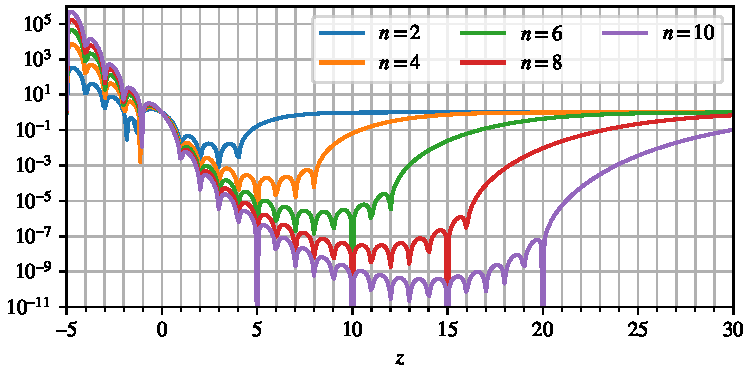
\includegraphics{papers/laguerre/images/rel_error_simple.pdf}
%\vspace{-12pt}
\caption{Relativer Fehler des direkten Ansatzes
für verschiedene reele Werte von $z$ und Grade $n$ der Laguerre-Polynome}
\label{laguerre:fig:rel_error_simple}
\end{figure}

Bevor wir die Gauss-Laguerre-Quadratur anwenden,
möchten wir als ersten Schritt eine Fehlerabschätzung durchführen.
Für den Fehlerterm \eqref{laguerre:lag_error} wird die $2n$-te Ableitung
der zu integrierenden Funktion $f(\xi)$ benötigt.
Für das Integral der Gamma-Funktion ergibt sich also
\begin{align*}
\frac{d^{2n}}{d\xi^{2n}} f(\xi)
 & =
\frac{d^{2n}}{d\xi^{2n}} \xi^{z-1}
\\
 & =
(z - 2n)_{2n} \xi^{z - 2n - 1}
.
\end{align*}
Eingesetzt im Fehlerterm \eqref{laguerre:lag_error} resultiert
\begin{align}
R_n
=
(z - 2n)_{2n} \frac{(n!)^2}{(2n)!} \xi^{z-2n-1}
,
\label{laguerre:gamma_err_simple}
\end{align}
wobei $\xi$ ein geeigneter Wert im Interval $(0, \infty)$ ist
und $n$ der Grad des verwendeten Laguerre-Polynoms.
Eine Fehlerabschätzung mit dem Fehlerterm stellt sich als unnütz heraus,
da $R_n$ für $z < 2n - 1$ bei $\xi \rightarrow 0$ eine Singularität aufweist
und für $z > 2n - 1$ bei $\xi \rightarrow \infty$ divergiert.
Nur für den unwahrscheinlichen Fall $ z = 2n - 1$
wäre eine Fehlerabschätzung plausibel.

Wenden wir nun also direkt die Gauss-Laguerre-Quadratur auf die Gamma-Funktion
an.
Dazu benötigen wir die Gewichte nach
\eqref{laguerre:quadratur_gewichte}
und als Stützstellen die Nullstellen des Laguerre-Polynomes $L_n$.
Evaluieren wir den relativen Fehler unserer Approximation zeigt sich ein
Bild wie in Abbildung~\ref{laguerre:fig:rel_error_simple}.
Man kann sehen,
wie der relative Fehler Nullstellen aufweist für ganzzahlige $z \leq 2n$.
Laut der Theorie der Gauss-Quadratur auch ist das zu erwarten,
da die Approximation via Gauss-Quadratur
exakt ist für zu integrierende Polynome mit Grad $\leq 2n-1$
und hinzukommt,
dass zudem von $z$ noch $1$ abgezogen wird im Exponenten.
Es ist ersichtlich,
dass sich für den Polynomgrad $n$ ein Interval gibt,
in dem der relative Fehler minimal ist.
Links steigt der relative Fehler besonders stark an,
während er auf der rechten Seite zu konvergieren scheint.
Um die linke Hälfte in den Griff zu bekommen,
könnten wir die Reflektionsformel der Gamma-Funktion ausnutzen.

\begin{figure}
\centering
% %% Creator: Matplotlib, PGF backend
%%
%% To include the figure in your LaTeX document, write
%%   \input{<filename>.pgf}
%%
%% Make sure the required packages are loaded in your preamble
%%   \usepackage{pgf}
%%
%% Also ensure that all the required font packages are loaded; for instance,
%% the lmodern package is sometimes necessary when using math font.
%%   \usepackage{lmodern}
%%
%% Figures using additional raster images can only be included by \input if
%% they are in the same directory as the main LaTeX file. For loading figures
%% from other directories you can use the `import` package
%%   \usepackage{import}
%%
%% and then include the figures with
%%   \import{<path to file>}{<filename>.pgf}
%%
%% Matplotlib used the following preamble
%%   \usepackage{fontspec}
%%   \setmainfont{DejaVuSerif.ttf}[Path=\detokenize{/home/mup/.local/lib/python3.8/site-packages/matplotlib/mpl-data/fonts/ttf/}]
%%   \setsansfont{DejaVuSans.ttf}[Path=\detokenize{/home/mup/.local/lib/python3.8/site-packages/matplotlib/mpl-data/fonts/ttf/}]
%%   \setmonofont{DejaVuSansMono.ttf}[Path=\detokenize{/home/mup/.local/lib/python3.8/site-packages/matplotlib/mpl-data/fonts/ttf/}]
%%
\begingroup%
\makeatletter%
\begin{pgfpicture}%
\pgfpathrectangle{\pgfpointorigin}{\pgfqpoint{5.000000in}{2.500000in}}%
\pgfusepath{use as bounding box, clip}%
\begin{pgfscope}%
\pgfsetbuttcap%
\pgfsetmiterjoin%
\definecolor{currentfill}{rgb}{1.000000,1.000000,1.000000}%
\pgfsetfillcolor{currentfill}%
\pgfsetlinewidth{0.000000pt}%
\definecolor{currentstroke}{rgb}{1.000000,1.000000,1.000000}%
\pgfsetstrokecolor{currentstroke}%
\pgfsetdash{}{0pt}%
\pgfpathmoveto{\pgfqpoint{0.000000in}{0.000000in}}%
\pgfpathlineto{\pgfqpoint{5.000000in}{0.000000in}}%
\pgfpathlineto{\pgfqpoint{5.000000in}{2.500000in}}%
\pgfpathlineto{\pgfqpoint{0.000000in}{2.500000in}}%
\pgfpathlineto{\pgfqpoint{0.000000in}{0.000000in}}%
\pgfpathclose%
\pgfusepath{fill}%
\end{pgfscope}%
\begin{pgfscope}%
\pgfsetbuttcap%
\pgfsetmiterjoin%
\definecolor{currentfill}{rgb}{1.000000,1.000000,1.000000}%
\pgfsetfillcolor{currentfill}%
\pgfsetlinewidth{0.000000pt}%
\definecolor{currentstroke}{rgb}{0.000000,0.000000,0.000000}%
\pgfsetstrokecolor{currentstroke}%
\pgfsetstrokeopacity{0.000000}%
\pgfsetdash{}{0pt}%
\pgfpathmoveto{\pgfqpoint{0.672226in}{0.463273in}}%
\pgfpathlineto{\pgfqpoint{4.869965in}{0.463273in}}%
\pgfpathlineto{\pgfqpoint{4.869965in}{2.458330in}}%
\pgfpathlineto{\pgfqpoint{0.672226in}{2.458330in}}%
\pgfpathlineto{\pgfqpoint{0.672226in}{0.463273in}}%
\pgfpathclose%
\pgfusepath{fill}%
\end{pgfscope}%
\begin{pgfscope}%
\pgfpathrectangle{\pgfqpoint{0.672226in}{0.463273in}}{\pgfqpoint{4.197739in}{1.995057in}}%
\pgfusepath{clip}%
\pgfsetrectcap%
\pgfsetroundjoin%
\pgfsetlinewidth{0.803000pt}%
\definecolor{currentstroke}{rgb}{0.690196,0.690196,0.690196}%
\pgfsetstrokecolor{currentstroke}%
\pgfsetdash{}{0pt}%
\pgfpathmoveto{\pgfqpoint{0.672226in}{0.463273in}}%
\pgfpathlineto{\pgfqpoint{0.672226in}{2.458330in}}%
\pgfusepath{stroke}%
\end{pgfscope}%
\begin{pgfscope}%
\pgfsetbuttcap%
\pgfsetroundjoin%
\definecolor{currentfill}{rgb}{0.000000,0.000000,0.000000}%
\pgfsetfillcolor{currentfill}%
\pgfsetlinewidth{0.803000pt}%
\definecolor{currentstroke}{rgb}{0.000000,0.000000,0.000000}%
\pgfsetstrokecolor{currentstroke}%
\pgfsetdash{}{0pt}%
\pgfsys@defobject{currentmarker}{\pgfqpoint{0.000000in}{-0.048611in}}{\pgfqpoint{0.000000in}{0.000000in}}{%
\pgfpathmoveto{\pgfqpoint{0.000000in}{0.000000in}}%
\pgfpathlineto{\pgfqpoint{0.000000in}{-0.048611in}}%
\pgfusepath{stroke,fill}%
}%
\begin{pgfscope}%
\pgfsys@transformshift{0.672226in}{0.463273in}%
\pgfsys@useobject{currentmarker}{}%
\end{pgfscope}%
\end{pgfscope}%
\begin{pgfscope}%
\definecolor{textcolor}{rgb}{0.000000,0.000000,0.000000}%
\pgfsetstrokecolor{textcolor}%
\pgfsetfillcolor{textcolor}%
\pgftext[x=0.672226in,y=0.366051in,,top]{\color{textcolor}\sffamily\fontsize{10.000000}{12.000000}\selectfont \ensuremath{-}15}%
\end{pgfscope}%
\begin{pgfscope}%
\pgfpathrectangle{\pgfqpoint{0.672226in}{0.463273in}}{\pgfqpoint{4.197739in}{1.995057in}}%
\pgfusepath{clip}%
\pgfsetrectcap%
\pgfsetroundjoin%
\pgfsetlinewidth{0.803000pt}%
\definecolor{currentstroke}{rgb}{0.690196,0.690196,0.690196}%
\pgfsetstrokecolor{currentstroke}%
\pgfsetdash{}{0pt}%
\pgfpathmoveto{\pgfqpoint{1.371849in}{0.463273in}}%
\pgfpathlineto{\pgfqpoint{1.371849in}{2.458330in}}%
\pgfusepath{stroke}%
\end{pgfscope}%
\begin{pgfscope}%
\pgfsetbuttcap%
\pgfsetroundjoin%
\definecolor{currentfill}{rgb}{0.000000,0.000000,0.000000}%
\pgfsetfillcolor{currentfill}%
\pgfsetlinewidth{0.803000pt}%
\definecolor{currentstroke}{rgb}{0.000000,0.000000,0.000000}%
\pgfsetstrokecolor{currentstroke}%
\pgfsetdash{}{0pt}%
\pgfsys@defobject{currentmarker}{\pgfqpoint{0.000000in}{-0.048611in}}{\pgfqpoint{0.000000in}{0.000000in}}{%
\pgfpathmoveto{\pgfqpoint{0.000000in}{0.000000in}}%
\pgfpathlineto{\pgfqpoint{0.000000in}{-0.048611in}}%
\pgfusepath{stroke,fill}%
}%
\begin{pgfscope}%
\pgfsys@transformshift{1.371849in}{0.463273in}%
\pgfsys@useobject{currentmarker}{}%
\end{pgfscope}%
\end{pgfscope}%
\begin{pgfscope}%
\definecolor{textcolor}{rgb}{0.000000,0.000000,0.000000}%
\pgfsetstrokecolor{textcolor}%
\pgfsetfillcolor{textcolor}%
\pgftext[x=1.371849in,y=0.366051in,,top]{\color{textcolor}\sffamily\fontsize{10.000000}{12.000000}\selectfont \ensuremath{-}10}%
\end{pgfscope}%
\begin{pgfscope}%
\pgfpathrectangle{\pgfqpoint{0.672226in}{0.463273in}}{\pgfqpoint{4.197739in}{1.995057in}}%
\pgfusepath{clip}%
\pgfsetrectcap%
\pgfsetroundjoin%
\pgfsetlinewidth{0.803000pt}%
\definecolor{currentstroke}{rgb}{0.690196,0.690196,0.690196}%
\pgfsetstrokecolor{currentstroke}%
\pgfsetdash{}{0pt}%
\pgfpathmoveto{\pgfqpoint{2.071472in}{0.463273in}}%
\pgfpathlineto{\pgfqpoint{2.071472in}{2.458330in}}%
\pgfusepath{stroke}%
\end{pgfscope}%
\begin{pgfscope}%
\pgfsetbuttcap%
\pgfsetroundjoin%
\definecolor{currentfill}{rgb}{0.000000,0.000000,0.000000}%
\pgfsetfillcolor{currentfill}%
\pgfsetlinewidth{0.803000pt}%
\definecolor{currentstroke}{rgb}{0.000000,0.000000,0.000000}%
\pgfsetstrokecolor{currentstroke}%
\pgfsetdash{}{0pt}%
\pgfsys@defobject{currentmarker}{\pgfqpoint{0.000000in}{-0.048611in}}{\pgfqpoint{0.000000in}{0.000000in}}{%
\pgfpathmoveto{\pgfqpoint{0.000000in}{0.000000in}}%
\pgfpathlineto{\pgfqpoint{0.000000in}{-0.048611in}}%
\pgfusepath{stroke,fill}%
}%
\begin{pgfscope}%
\pgfsys@transformshift{2.071472in}{0.463273in}%
\pgfsys@useobject{currentmarker}{}%
\end{pgfscope}%
\end{pgfscope}%
\begin{pgfscope}%
\definecolor{textcolor}{rgb}{0.000000,0.000000,0.000000}%
\pgfsetstrokecolor{textcolor}%
\pgfsetfillcolor{textcolor}%
\pgftext[x=2.071472in,y=0.366051in,,top]{\color{textcolor}\sffamily\fontsize{10.000000}{12.000000}\selectfont \ensuremath{-}5}%
\end{pgfscope}%
\begin{pgfscope}%
\pgfpathrectangle{\pgfqpoint{0.672226in}{0.463273in}}{\pgfqpoint{4.197739in}{1.995057in}}%
\pgfusepath{clip}%
\pgfsetrectcap%
\pgfsetroundjoin%
\pgfsetlinewidth{0.803000pt}%
\definecolor{currentstroke}{rgb}{0.690196,0.690196,0.690196}%
\pgfsetstrokecolor{currentstroke}%
\pgfsetdash{}{0pt}%
\pgfpathmoveto{\pgfqpoint{2.771095in}{0.463273in}}%
\pgfpathlineto{\pgfqpoint{2.771095in}{2.458330in}}%
\pgfusepath{stroke}%
\end{pgfscope}%
\begin{pgfscope}%
\pgfsetbuttcap%
\pgfsetroundjoin%
\definecolor{currentfill}{rgb}{0.000000,0.000000,0.000000}%
\pgfsetfillcolor{currentfill}%
\pgfsetlinewidth{0.803000pt}%
\definecolor{currentstroke}{rgb}{0.000000,0.000000,0.000000}%
\pgfsetstrokecolor{currentstroke}%
\pgfsetdash{}{0pt}%
\pgfsys@defobject{currentmarker}{\pgfqpoint{0.000000in}{-0.048611in}}{\pgfqpoint{0.000000in}{0.000000in}}{%
\pgfpathmoveto{\pgfqpoint{0.000000in}{0.000000in}}%
\pgfpathlineto{\pgfqpoint{0.000000in}{-0.048611in}}%
\pgfusepath{stroke,fill}%
}%
\begin{pgfscope}%
\pgfsys@transformshift{2.771095in}{0.463273in}%
\pgfsys@useobject{currentmarker}{}%
\end{pgfscope}%
\end{pgfscope}%
\begin{pgfscope}%
\definecolor{textcolor}{rgb}{0.000000,0.000000,0.000000}%
\pgfsetstrokecolor{textcolor}%
\pgfsetfillcolor{textcolor}%
\pgftext[x=2.771095in,y=0.366051in,,top]{\color{textcolor}\sffamily\fontsize{10.000000}{12.000000}\selectfont 0}%
\end{pgfscope}%
\begin{pgfscope}%
\pgfpathrectangle{\pgfqpoint{0.672226in}{0.463273in}}{\pgfqpoint{4.197739in}{1.995057in}}%
\pgfusepath{clip}%
\pgfsetrectcap%
\pgfsetroundjoin%
\pgfsetlinewidth{0.803000pt}%
\definecolor{currentstroke}{rgb}{0.690196,0.690196,0.690196}%
\pgfsetstrokecolor{currentstroke}%
\pgfsetdash{}{0pt}%
\pgfpathmoveto{\pgfqpoint{3.470718in}{0.463273in}}%
\pgfpathlineto{\pgfqpoint{3.470718in}{2.458330in}}%
\pgfusepath{stroke}%
\end{pgfscope}%
\begin{pgfscope}%
\pgfsetbuttcap%
\pgfsetroundjoin%
\definecolor{currentfill}{rgb}{0.000000,0.000000,0.000000}%
\pgfsetfillcolor{currentfill}%
\pgfsetlinewidth{0.803000pt}%
\definecolor{currentstroke}{rgb}{0.000000,0.000000,0.000000}%
\pgfsetstrokecolor{currentstroke}%
\pgfsetdash{}{0pt}%
\pgfsys@defobject{currentmarker}{\pgfqpoint{0.000000in}{-0.048611in}}{\pgfqpoint{0.000000in}{0.000000in}}{%
\pgfpathmoveto{\pgfqpoint{0.000000in}{0.000000in}}%
\pgfpathlineto{\pgfqpoint{0.000000in}{-0.048611in}}%
\pgfusepath{stroke,fill}%
}%
\begin{pgfscope}%
\pgfsys@transformshift{3.470718in}{0.463273in}%
\pgfsys@useobject{currentmarker}{}%
\end{pgfscope}%
\end{pgfscope}%
\begin{pgfscope}%
\definecolor{textcolor}{rgb}{0.000000,0.000000,0.000000}%
\pgfsetstrokecolor{textcolor}%
\pgfsetfillcolor{textcolor}%
\pgftext[x=3.470718in,y=0.366051in,,top]{\color{textcolor}\sffamily\fontsize{10.000000}{12.000000}\selectfont 5}%
\end{pgfscope}%
\begin{pgfscope}%
\pgfpathrectangle{\pgfqpoint{0.672226in}{0.463273in}}{\pgfqpoint{4.197739in}{1.995057in}}%
\pgfusepath{clip}%
\pgfsetrectcap%
\pgfsetroundjoin%
\pgfsetlinewidth{0.803000pt}%
\definecolor{currentstroke}{rgb}{0.690196,0.690196,0.690196}%
\pgfsetstrokecolor{currentstroke}%
\pgfsetdash{}{0pt}%
\pgfpathmoveto{\pgfqpoint{4.170342in}{0.463273in}}%
\pgfpathlineto{\pgfqpoint{4.170342in}{2.458330in}}%
\pgfusepath{stroke}%
\end{pgfscope}%
\begin{pgfscope}%
\pgfsetbuttcap%
\pgfsetroundjoin%
\definecolor{currentfill}{rgb}{0.000000,0.000000,0.000000}%
\pgfsetfillcolor{currentfill}%
\pgfsetlinewidth{0.803000pt}%
\definecolor{currentstroke}{rgb}{0.000000,0.000000,0.000000}%
\pgfsetstrokecolor{currentstroke}%
\pgfsetdash{}{0pt}%
\pgfsys@defobject{currentmarker}{\pgfqpoint{0.000000in}{-0.048611in}}{\pgfqpoint{0.000000in}{0.000000in}}{%
\pgfpathmoveto{\pgfqpoint{0.000000in}{0.000000in}}%
\pgfpathlineto{\pgfqpoint{0.000000in}{-0.048611in}}%
\pgfusepath{stroke,fill}%
}%
\begin{pgfscope}%
\pgfsys@transformshift{4.170342in}{0.463273in}%
\pgfsys@useobject{currentmarker}{}%
\end{pgfscope}%
\end{pgfscope}%
\begin{pgfscope}%
\definecolor{textcolor}{rgb}{0.000000,0.000000,0.000000}%
\pgfsetstrokecolor{textcolor}%
\pgfsetfillcolor{textcolor}%
\pgftext[x=4.170342in,y=0.366051in,,top]{\color{textcolor}\sffamily\fontsize{10.000000}{12.000000}\selectfont 10}%
\end{pgfscope}%
\begin{pgfscope}%
\pgfpathrectangle{\pgfqpoint{0.672226in}{0.463273in}}{\pgfqpoint{4.197739in}{1.995057in}}%
\pgfusepath{clip}%
\pgfsetrectcap%
\pgfsetroundjoin%
\pgfsetlinewidth{0.803000pt}%
\definecolor{currentstroke}{rgb}{0.690196,0.690196,0.690196}%
\pgfsetstrokecolor{currentstroke}%
\pgfsetdash{}{0pt}%
\pgfpathmoveto{\pgfqpoint{4.869965in}{0.463273in}}%
\pgfpathlineto{\pgfqpoint{4.869965in}{2.458330in}}%
\pgfusepath{stroke}%
\end{pgfscope}%
\begin{pgfscope}%
\pgfsetbuttcap%
\pgfsetroundjoin%
\definecolor{currentfill}{rgb}{0.000000,0.000000,0.000000}%
\pgfsetfillcolor{currentfill}%
\pgfsetlinewidth{0.803000pt}%
\definecolor{currentstroke}{rgb}{0.000000,0.000000,0.000000}%
\pgfsetstrokecolor{currentstroke}%
\pgfsetdash{}{0pt}%
\pgfsys@defobject{currentmarker}{\pgfqpoint{0.000000in}{-0.048611in}}{\pgfqpoint{0.000000in}{0.000000in}}{%
\pgfpathmoveto{\pgfqpoint{0.000000in}{0.000000in}}%
\pgfpathlineto{\pgfqpoint{0.000000in}{-0.048611in}}%
\pgfusepath{stroke,fill}%
}%
\begin{pgfscope}%
\pgfsys@transformshift{4.869965in}{0.463273in}%
\pgfsys@useobject{currentmarker}{}%
\end{pgfscope}%
\end{pgfscope}%
\begin{pgfscope}%
\definecolor{textcolor}{rgb}{0.000000,0.000000,0.000000}%
\pgfsetstrokecolor{textcolor}%
\pgfsetfillcolor{textcolor}%
\pgftext[x=4.869965in,y=0.366051in,,top]{\color{textcolor}\sffamily\fontsize{10.000000}{12.000000}\selectfont 15}%
\end{pgfscope}%
\begin{pgfscope}%
\pgfpathrectangle{\pgfqpoint{0.672226in}{0.463273in}}{\pgfqpoint{4.197739in}{1.995057in}}%
\pgfusepath{clip}%
\pgfsetrectcap%
\pgfsetroundjoin%
\pgfsetlinewidth{0.803000pt}%
\definecolor{currentstroke}{rgb}{0.690196,0.690196,0.690196}%
\pgfsetstrokecolor{currentstroke}%
\pgfsetdash{}{0pt}%
\pgfpathmoveto{\pgfqpoint{0.812150in}{0.463273in}}%
\pgfpathlineto{\pgfqpoint{0.812150in}{2.458330in}}%
\pgfusepath{stroke}%
\end{pgfscope}%
\begin{pgfscope}%
\pgfsetbuttcap%
\pgfsetroundjoin%
\definecolor{currentfill}{rgb}{0.000000,0.000000,0.000000}%
\pgfsetfillcolor{currentfill}%
\pgfsetlinewidth{0.602250pt}%
\definecolor{currentstroke}{rgb}{0.000000,0.000000,0.000000}%
\pgfsetstrokecolor{currentstroke}%
\pgfsetdash{}{0pt}%
\pgfsys@defobject{currentmarker}{\pgfqpoint{0.000000in}{-0.027778in}}{\pgfqpoint{0.000000in}{0.000000in}}{%
\pgfpathmoveto{\pgfqpoint{0.000000in}{0.000000in}}%
\pgfpathlineto{\pgfqpoint{0.000000in}{-0.027778in}}%
\pgfusepath{stroke,fill}%
}%
\begin{pgfscope}%
\pgfsys@transformshift{0.812150in}{0.463273in}%
\pgfsys@useobject{currentmarker}{}%
\end{pgfscope}%
\end{pgfscope}%
\begin{pgfscope}%
\pgfpathrectangle{\pgfqpoint{0.672226in}{0.463273in}}{\pgfqpoint{4.197739in}{1.995057in}}%
\pgfusepath{clip}%
\pgfsetrectcap%
\pgfsetroundjoin%
\pgfsetlinewidth{0.803000pt}%
\definecolor{currentstroke}{rgb}{0.690196,0.690196,0.690196}%
\pgfsetstrokecolor{currentstroke}%
\pgfsetdash{}{0pt}%
\pgfpathmoveto{\pgfqpoint{0.952075in}{0.463273in}}%
\pgfpathlineto{\pgfqpoint{0.952075in}{2.458330in}}%
\pgfusepath{stroke}%
\end{pgfscope}%
\begin{pgfscope}%
\pgfsetbuttcap%
\pgfsetroundjoin%
\definecolor{currentfill}{rgb}{0.000000,0.000000,0.000000}%
\pgfsetfillcolor{currentfill}%
\pgfsetlinewidth{0.602250pt}%
\definecolor{currentstroke}{rgb}{0.000000,0.000000,0.000000}%
\pgfsetstrokecolor{currentstroke}%
\pgfsetdash{}{0pt}%
\pgfsys@defobject{currentmarker}{\pgfqpoint{0.000000in}{-0.027778in}}{\pgfqpoint{0.000000in}{0.000000in}}{%
\pgfpathmoveto{\pgfqpoint{0.000000in}{0.000000in}}%
\pgfpathlineto{\pgfqpoint{0.000000in}{-0.027778in}}%
\pgfusepath{stroke,fill}%
}%
\begin{pgfscope}%
\pgfsys@transformshift{0.952075in}{0.463273in}%
\pgfsys@useobject{currentmarker}{}%
\end{pgfscope}%
\end{pgfscope}%
\begin{pgfscope}%
\pgfpathrectangle{\pgfqpoint{0.672226in}{0.463273in}}{\pgfqpoint{4.197739in}{1.995057in}}%
\pgfusepath{clip}%
\pgfsetrectcap%
\pgfsetroundjoin%
\pgfsetlinewidth{0.803000pt}%
\definecolor{currentstroke}{rgb}{0.690196,0.690196,0.690196}%
\pgfsetstrokecolor{currentstroke}%
\pgfsetdash{}{0pt}%
\pgfpathmoveto{\pgfqpoint{1.092000in}{0.463273in}}%
\pgfpathlineto{\pgfqpoint{1.092000in}{2.458330in}}%
\pgfusepath{stroke}%
\end{pgfscope}%
\begin{pgfscope}%
\pgfsetbuttcap%
\pgfsetroundjoin%
\definecolor{currentfill}{rgb}{0.000000,0.000000,0.000000}%
\pgfsetfillcolor{currentfill}%
\pgfsetlinewidth{0.602250pt}%
\definecolor{currentstroke}{rgb}{0.000000,0.000000,0.000000}%
\pgfsetstrokecolor{currentstroke}%
\pgfsetdash{}{0pt}%
\pgfsys@defobject{currentmarker}{\pgfqpoint{0.000000in}{-0.027778in}}{\pgfqpoint{0.000000in}{0.000000in}}{%
\pgfpathmoveto{\pgfqpoint{0.000000in}{0.000000in}}%
\pgfpathlineto{\pgfqpoint{0.000000in}{-0.027778in}}%
\pgfusepath{stroke,fill}%
}%
\begin{pgfscope}%
\pgfsys@transformshift{1.092000in}{0.463273in}%
\pgfsys@useobject{currentmarker}{}%
\end{pgfscope}%
\end{pgfscope}%
\begin{pgfscope}%
\pgfpathrectangle{\pgfqpoint{0.672226in}{0.463273in}}{\pgfqpoint{4.197739in}{1.995057in}}%
\pgfusepath{clip}%
\pgfsetrectcap%
\pgfsetroundjoin%
\pgfsetlinewidth{0.803000pt}%
\definecolor{currentstroke}{rgb}{0.690196,0.690196,0.690196}%
\pgfsetstrokecolor{currentstroke}%
\pgfsetdash{}{0pt}%
\pgfpathmoveto{\pgfqpoint{1.231924in}{0.463273in}}%
\pgfpathlineto{\pgfqpoint{1.231924in}{2.458330in}}%
\pgfusepath{stroke}%
\end{pgfscope}%
\begin{pgfscope}%
\pgfsetbuttcap%
\pgfsetroundjoin%
\definecolor{currentfill}{rgb}{0.000000,0.000000,0.000000}%
\pgfsetfillcolor{currentfill}%
\pgfsetlinewidth{0.602250pt}%
\definecolor{currentstroke}{rgb}{0.000000,0.000000,0.000000}%
\pgfsetstrokecolor{currentstroke}%
\pgfsetdash{}{0pt}%
\pgfsys@defobject{currentmarker}{\pgfqpoint{0.000000in}{-0.027778in}}{\pgfqpoint{0.000000in}{0.000000in}}{%
\pgfpathmoveto{\pgfqpoint{0.000000in}{0.000000in}}%
\pgfpathlineto{\pgfqpoint{0.000000in}{-0.027778in}}%
\pgfusepath{stroke,fill}%
}%
\begin{pgfscope}%
\pgfsys@transformshift{1.231924in}{0.463273in}%
\pgfsys@useobject{currentmarker}{}%
\end{pgfscope}%
\end{pgfscope}%
\begin{pgfscope}%
\pgfpathrectangle{\pgfqpoint{0.672226in}{0.463273in}}{\pgfqpoint{4.197739in}{1.995057in}}%
\pgfusepath{clip}%
\pgfsetrectcap%
\pgfsetroundjoin%
\pgfsetlinewidth{0.803000pt}%
\definecolor{currentstroke}{rgb}{0.690196,0.690196,0.690196}%
\pgfsetstrokecolor{currentstroke}%
\pgfsetdash{}{0pt}%
\pgfpathmoveto{\pgfqpoint{1.511774in}{0.463273in}}%
\pgfpathlineto{\pgfqpoint{1.511774in}{2.458330in}}%
\pgfusepath{stroke}%
\end{pgfscope}%
\begin{pgfscope}%
\pgfsetbuttcap%
\pgfsetroundjoin%
\definecolor{currentfill}{rgb}{0.000000,0.000000,0.000000}%
\pgfsetfillcolor{currentfill}%
\pgfsetlinewidth{0.602250pt}%
\definecolor{currentstroke}{rgb}{0.000000,0.000000,0.000000}%
\pgfsetstrokecolor{currentstroke}%
\pgfsetdash{}{0pt}%
\pgfsys@defobject{currentmarker}{\pgfqpoint{0.000000in}{-0.027778in}}{\pgfqpoint{0.000000in}{0.000000in}}{%
\pgfpathmoveto{\pgfqpoint{0.000000in}{0.000000in}}%
\pgfpathlineto{\pgfqpoint{0.000000in}{-0.027778in}}%
\pgfusepath{stroke,fill}%
}%
\begin{pgfscope}%
\pgfsys@transformshift{1.511774in}{0.463273in}%
\pgfsys@useobject{currentmarker}{}%
\end{pgfscope}%
\end{pgfscope}%
\begin{pgfscope}%
\pgfpathrectangle{\pgfqpoint{0.672226in}{0.463273in}}{\pgfqpoint{4.197739in}{1.995057in}}%
\pgfusepath{clip}%
\pgfsetrectcap%
\pgfsetroundjoin%
\pgfsetlinewidth{0.803000pt}%
\definecolor{currentstroke}{rgb}{0.690196,0.690196,0.690196}%
\pgfsetstrokecolor{currentstroke}%
\pgfsetdash{}{0pt}%
\pgfpathmoveto{\pgfqpoint{1.651698in}{0.463273in}}%
\pgfpathlineto{\pgfqpoint{1.651698in}{2.458330in}}%
\pgfusepath{stroke}%
\end{pgfscope}%
\begin{pgfscope}%
\pgfsetbuttcap%
\pgfsetroundjoin%
\definecolor{currentfill}{rgb}{0.000000,0.000000,0.000000}%
\pgfsetfillcolor{currentfill}%
\pgfsetlinewidth{0.602250pt}%
\definecolor{currentstroke}{rgb}{0.000000,0.000000,0.000000}%
\pgfsetstrokecolor{currentstroke}%
\pgfsetdash{}{0pt}%
\pgfsys@defobject{currentmarker}{\pgfqpoint{0.000000in}{-0.027778in}}{\pgfqpoint{0.000000in}{0.000000in}}{%
\pgfpathmoveto{\pgfqpoint{0.000000in}{0.000000in}}%
\pgfpathlineto{\pgfqpoint{0.000000in}{-0.027778in}}%
\pgfusepath{stroke,fill}%
}%
\begin{pgfscope}%
\pgfsys@transformshift{1.651698in}{0.463273in}%
\pgfsys@useobject{currentmarker}{}%
\end{pgfscope}%
\end{pgfscope}%
\begin{pgfscope}%
\pgfpathrectangle{\pgfqpoint{0.672226in}{0.463273in}}{\pgfqpoint{4.197739in}{1.995057in}}%
\pgfusepath{clip}%
\pgfsetrectcap%
\pgfsetroundjoin%
\pgfsetlinewidth{0.803000pt}%
\definecolor{currentstroke}{rgb}{0.690196,0.690196,0.690196}%
\pgfsetstrokecolor{currentstroke}%
\pgfsetdash{}{0pt}%
\pgfpathmoveto{\pgfqpoint{1.791623in}{0.463273in}}%
\pgfpathlineto{\pgfqpoint{1.791623in}{2.458330in}}%
\pgfusepath{stroke}%
\end{pgfscope}%
\begin{pgfscope}%
\pgfsetbuttcap%
\pgfsetroundjoin%
\definecolor{currentfill}{rgb}{0.000000,0.000000,0.000000}%
\pgfsetfillcolor{currentfill}%
\pgfsetlinewidth{0.602250pt}%
\definecolor{currentstroke}{rgb}{0.000000,0.000000,0.000000}%
\pgfsetstrokecolor{currentstroke}%
\pgfsetdash{}{0pt}%
\pgfsys@defobject{currentmarker}{\pgfqpoint{0.000000in}{-0.027778in}}{\pgfqpoint{0.000000in}{0.000000in}}{%
\pgfpathmoveto{\pgfqpoint{0.000000in}{0.000000in}}%
\pgfpathlineto{\pgfqpoint{0.000000in}{-0.027778in}}%
\pgfusepath{stroke,fill}%
}%
\begin{pgfscope}%
\pgfsys@transformshift{1.791623in}{0.463273in}%
\pgfsys@useobject{currentmarker}{}%
\end{pgfscope}%
\end{pgfscope}%
\begin{pgfscope}%
\pgfpathrectangle{\pgfqpoint{0.672226in}{0.463273in}}{\pgfqpoint{4.197739in}{1.995057in}}%
\pgfusepath{clip}%
\pgfsetrectcap%
\pgfsetroundjoin%
\pgfsetlinewidth{0.803000pt}%
\definecolor{currentstroke}{rgb}{0.690196,0.690196,0.690196}%
\pgfsetstrokecolor{currentstroke}%
\pgfsetdash{}{0pt}%
\pgfpathmoveto{\pgfqpoint{1.931547in}{0.463273in}}%
\pgfpathlineto{\pgfqpoint{1.931547in}{2.458330in}}%
\pgfusepath{stroke}%
\end{pgfscope}%
\begin{pgfscope}%
\pgfsetbuttcap%
\pgfsetroundjoin%
\definecolor{currentfill}{rgb}{0.000000,0.000000,0.000000}%
\pgfsetfillcolor{currentfill}%
\pgfsetlinewidth{0.602250pt}%
\definecolor{currentstroke}{rgb}{0.000000,0.000000,0.000000}%
\pgfsetstrokecolor{currentstroke}%
\pgfsetdash{}{0pt}%
\pgfsys@defobject{currentmarker}{\pgfqpoint{0.000000in}{-0.027778in}}{\pgfqpoint{0.000000in}{0.000000in}}{%
\pgfpathmoveto{\pgfqpoint{0.000000in}{0.000000in}}%
\pgfpathlineto{\pgfqpoint{0.000000in}{-0.027778in}}%
\pgfusepath{stroke,fill}%
}%
\begin{pgfscope}%
\pgfsys@transformshift{1.931547in}{0.463273in}%
\pgfsys@useobject{currentmarker}{}%
\end{pgfscope}%
\end{pgfscope}%
\begin{pgfscope}%
\pgfpathrectangle{\pgfqpoint{0.672226in}{0.463273in}}{\pgfqpoint{4.197739in}{1.995057in}}%
\pgfusepath{clip}%
\pgfsetrectcap%
\pgfsetroundjoin%
\pgfsetlinewidth{0.803000pt}%
\definecolor{currentstroke}{rgb}{0.690196,0.690196,0.690196}%
\pgfsetstrokecolor{currentstroke}%
\pgfsetdash{}{0pt}%
\pgfpathmoveto{\pgfqpoint{2.211397in}{0.463273in}}%
\pgfpathlineto{\pgfqpoint{2.211397in}{2.458330in}}%
\pgfusepath{stroke}%
\end{pgfscope}%
\begin{pgfscope}%
\pgfsetbuttcap%
\pgfsetroundjoin%
\definecolor{currentfill}{rgb}{0.000000,0.000000,0.000000}%
\pgfsetfillcolor{currentfill}%
\pgfsetlinewidth{0.602250pt}%
\definecolor{currentstroke}{rgb}{0.000000,0.000000,0.000000}%
\pgfsetstrokecolor{currentstroke}%
\pgfsetdash{}{0pt}%
\pgfsys@defobject{currentmarker}{\pgfqpoint{0.000000in}{-0.027778in}}{\pgfqpoint{0.000000in}{0.000000in}}{%
\pgfpathmoveto{\pgfqpoint{0.000000in}{0.000000in}}%
\pgfpathlineto{\pgfqpoint{0.000000in}{-0.027778in}}%
\pgfusepath{stroke,fill}%
}%
\begin{pgfscope}%
\pgfsys@transformshift{2.211397in}{0.463273in}%
\pgfsys@useobject{currentmarker}{}%
\end{pgfscope}%
\end{pgfscope}%
\begin{pgfscope}%
\pgfpathrectangle{\pgfqpoint{0.672226in}{0.463273in}}{\pgfqpoint{4.197739in}{1.995057in}}%
\pgfusepath{clip}%
\pgfsetrectcap%
\pgfsetroundjoin%
\pgfsetlinewidth{0.803000pt}%
\definecolor{currentstroke}{rgb}{0.690196,0.690196,0.690196}%
\pgfsetstrokecolor{currentstroke}%
\pgfsetdash{}{0pt}%
\pgfpathmoveto{\pgfqpoint{2.351321in}{0.463273in}}%
\pgfpathlineto{\pgfqpoint{2.351321in}{2.458330in}}%
\pgfusepath{stroke}%
\end{pgfscope}%
\begin{pgfscope}%
\pgfsetbuttcap%
\pgfsetroundjoin%
\definecolor{currentfill}{rgb}{0.000000,0.000000,0.000000}%
\pgfsetfillcolor{currentfill}%
\pgfsetlinewidth{0.602250pt}%
\definecolor{currentstroke}{rgb}{0.000000,0.000000,0.000000}%
\pgfsetstrokecolor{currentstroke}%
\pgfsetdash{}{0pt}%
\pgfsys@defobject{currentmarker}{\pgfqpoint{0.000000in}{-0.027778in}}{\pgfqpoint{0.000000in}{0.000000in}}{%
\pgfpathmoveto{\pgfqpoint{0.000000in}{0.000000in}}%
\pgfpathlineto{\pgfqpoint{0.000000in}{-0.027778in}}%
\pgfusepath{stroke,fill}%
}%
\begin{pgfscope}%
\pgfsys@transformshift{2.351321in}{0.463273in}%
\pgfsys@useobject{currentmarker}{}%
\end{pgfscope}%
\end{pgfscope}%
\begin{pgfscope}%
\pgfpathrectangle{\pgfqpoint{0.672226in}{0.463273in}}{\pgfqpoint{4.197739in}{1.995057in}}%
\pgfusepath{clip}%
\pgfsetrectcap%
\pgfsetroundjoin%
\pgfsetlinewidth{0.803000pt}%
\definecolor{currentstroke}{rgb}{0.690196,0.690196,0.690196}%
\pgfsetstrokecolor{currentstroke}%
\pgfsetdash{}{0pt}%
\pgfpathmoveto{\pgfqpoint{2.491246in}{0.463273in}}%
\pgfpathlineto{\pgfqpoint{2.491246in}{2.458330in}}%
\pgfusepath{stroke}%
\end{pgfscope}%
\begin{pgfscope}%
\pgfsetbuttcap%
\pgfsetroundjoin%
\definecolor{currentfill}{rgb}{0.000000,0.000000,0.000000}%
\pgfsetfillcolor{currentfill}%
\pgfsetlinewidth{0.602250pt}%
\definecolor{currentstroke}{rgb}{0.000000,0.000000,0.000000}%
\pgfsetstrokecolor{currentstroke}%
\pgfsetdash{}{0pt}%
\pgfsys@defobject{currentmarker}{\pgfqpoint{0.000000in}{-0.027778in}}{\pgfqpoint{0.000000in}{0.000000in}}{%
\pgfpathmoveto{\pgfqpoint{0.000000in}{0.000000in}}%
\pgfpathlineto{\pgfqpoint{0.000000in}{-0.027778in}}%
\pgfusepath{stroke,fill}%
}%
\begin{pgfscope}%
\pgfsys@transformshift{2.491246in}{0.463273in}%
\pgfsys@useobject{currentmarker}{}%
\end{pgfscope}%
\end{pgfscope}%
\begin{pgfscope}%
\pgfpathrectangle{\pgfqpoint{0.672226in}{0.463273in}}{\pgfqpoint{4.197739in}{1.995057in}}%
\pgfusepath{clip}%
\pgfsetrectcap%
\pgfsetroundjoin%
\pgfsetlinewidth{0.803000pt}%
\definecolor{currentstroke}{rgb}{0.690196,0.690196,0.690196}%
\pgfsetstrokecolor{currentstroke}%
\pgfsetdash{}{0pt}%
\pgfpathmoveto{\pgfqpoint{2.631171in}{0.463273in}}%
\pgfpathlineto{\pgfqpoint{2.631171in}{2.458330in}}%
\pgfusepath{stroke}%
\end{pgfscope}%
\begin{pgfscope}%
\pgfsetbuttcap%
\pgfsetroundjoin%
\definecolor{currentfill}{rgb}{0.000000,0.000000,0.000000}%
\pgfsetfillcolor{currentfill}%
\pgfsetlinewidth{0.602250pt}%
\definecolor{currentstroke}{rgb}{0.000000,0.000000,0.000000}%
\pgfsetstrokecolor{currentstroke}%
\pgfsetdash{}{0pt}%
\pgfsys@defobject{currentmarker}{\pgfqpoint{0.000000in}{-0.027778in}}{\pgfqpoint{0.000000in}{0.000000in}}{%
\pgfpathmoveto{\pgfqpoint{0.000000in}{0.000000in}}%
\pgfpathlineto{\pgfqpoint{0.000000in}{-0.027778in}}%
\pgfusepath{stroke,fill}%
}%
\begin{pgfscope}%
\pgfsys@transformshift{2.631171in}{0.463273in}%
\pgfsys@useobject{currentmarker}{}%
\end{pgfscope}%
\end{pgfscope}%
\begin{pgfscope}%
\pgfpathrectangle{\pgfqpoint{0.672226in}{0.463273in}}{\pgfqpoint{4.197739in}{1.995057in}}%
\pgfusepath{clip}%
\pgfsetrectcap%
\pgfsetroundjoin%
\pgfsetlinewidth{0.803000pt}%
\definecolor{currentstroke}{rgb}{0.690196,0.690196,0.690196}%
\pgfsetstrokecolor{currentstroke}%
\pgfsetdash{}{0pt}%
\pgfpathmoveto{\pgfqpoint{2.911020in}{0.463273in}}%
\pgfpathlineto{\pgfqpoint{2.911020in}{2.458330in}}%
\pgfusepath{stroke}%
\end{pgfscope}%
\begin{pgfscope}%
\pgfsetbuttcap%
\pgfsetroundjoin%
\definecolor{currentfill}{rgb}{0.000000,0.000000,0.000000}%
\pgfsetfillcolor{currentfill}%
\pgfsetlinewidth{0.602250pt}%
\definecolor{currentstroke}{rgb}{0.000000,0.000000,0.000000}%
\pgfsetstrokecolor{currentstroke}%
\pgfsetdash{}{0pt}%
\pgfsys@defobject{currentmarker}{\pgfqpoint{0.000000in}{-0.027778in}}{\pgfqpoint{0.000000in}{0.000000in}}{%
\pgfpathmoveto{\pgfqpoint{0.000000in}{0.000000in}}%
\pgfpathlineto{\pgfqpoint{0.000000in}{-0.027778in}}%
\pgfusepath{stroke,fill}%
}%
\begin{pgfscope}%
\pgfsys@transformshift{2.911020in}{0.463273in}%
\pgfsys@useobject{currentmarker}{}%
\end{pgfscope}%
\end{pgfscope}%
\begin{pgfscope}%
\pgfpathrectangle{\pgfqpoint{0.672226in}{0.463273in}}{\pgfqpoint{4.197739in}{1.995057in}}%
\pgfusepath{clip}%
\pgfsetrectcap%
\pgfsetroundjoin%
\pgfsetlinewidth{0.803000pt}%
\definecolor{currentstroke}{rgb}{0.690196,0.690196,0.690196}%
\pgfsetstrokecolor{currentstroke}%
\pgfsetdash{}{0pt}%
\pgfpathmoveto{\pgfqpoint{3.050944in}{0.463273in}}%
\pgfpathlineto{\pgfqpoint{3.050944in}{2.458330in}}%
\pgfusepath{stroke}%
\end{pgfscope}%
\begin{pgfscope}%
\pgfsetbuttcap%
\pgfsetroundjoin%
\definecolor{currentfill}{rgb}{0.000000,0.000000,0.000000}%
\pgfsetfillcolor{currentfill}%
\pgfsetlinewidth{0.602250pt}%
\definecolor{currentstroke}{rgb}{0.000000,0.000000,0.000000}%
\pgfsetstrokecolor{currentstroke}%
\pgfsetdash{}{0pt}%
\pgfsys@defobject{currentmarker}{\pgfqpoint{0.000000in}{-0.027778in}}{\pgfqpoint{0.000000in}{0.000000in}}{%
\pgfpathmoveto{\pgfqpoint{0.000000in}{0.000000in}}%
\pgfpathlineto{\pgfqpoint{0.000000in}{-0.027778in}}%
\pgfusepath{stroke,fill}%
}%
\begin{pgfscope}%
\pgfsys@transformshift{3.050944in}{0.463273in}%
\pgfsys@useobject{currentmarker}{}%
\end{pgfscope}%
\end{pgfscope}%
\begin{pgfscope}%
\pgfpathrectangle{\pgfqpoint{0.672226in}{0.463273in}}{\pgfqpoint{4.197739in}{1.995057in}}%
\pgfusepath{clip}%
\pgfsetrectcap%
\pgfsetroundjoin%
\pgfsetlinewidth{0.803000pt}%
\definecolor{currentstroke}{rgb}{0.690196,0.690196,0.690196}%
\pgfsetstrokecolor{currentstroke}%
\pgfsetdash{}{0pt}%
\pgfpathmoveto{\pgfqpoint{3.190869in}{0.463273in}}%
\pgfpathlineto{\pgfqpoint{3.190869in}{2.458330in}}%
\pgfusepath{stroke}%
\end{pgfscope}%
\begin{pgfscope}%
\pgfsetbuttcap%
\pgfsetroundjoin%
\definecolor{currentfill}{rgb}{0.000000,0.000000,0.000000}%
\pgfsetfillcolor{currentfill}%
\pgfsetlinewidth{0.602250pt}%
\definecolor{currentstroke}{rgb}{0.000000,0.000000,0.000000}%
\pgfsetstrokecolor{currentstroke}%
\pgfsetdash{}{0pt}%
\pgfsys@defobject{currentmarker}{\pgfqpoint{0.000000in}{-0.027778in}}{\pgfqpoint{0.000000in}{0.000000in}}{%
\pgfpathmoveto{\pgfqpoint{0.000000in}{0.000000in}}%
\pgfpathlineto{\pgfqpoint{0.000000in}{-0.027778in}}%
\pgfusepath{stroke,fill}%
}%
\begin{pgfscope}%
\pgfsys@transformshift{3.190869in}{0.463273in}%
\pgfsys@useobject{currentmarker}{}%
\end{pgfscope}%
\end{pgfscope}%
\begin{pgfscope}%
\pgfpathrectangle{\pgfqpoint{0.672226in}{0.463273in}}{\pgfqpoint{4.197739in}{1.995057in}}%
\pgfusepath{clip}%
\pgfsetrectcap%
\pgfsetroundjoin%
\pgfsetlinewidth{0.803000pt}%
\definecolor{currentstroke}{rgb}{0.690196,0.690196,0.690196}%
\pgfsetstrokecolor{currentstroke}%
\pgfsetdash{}{0pt}%
\pgfpathmoveto{\pgfqpoint{3.330794in}{0.463273in}}%
\pgfpathlineto{\pgfqpoint{3.330794in}{2.458330in}}%
\pgfusepath{stroke}%
\end{pgfscope}%
\begin{pgfscope}%
\pgfsetbuttcap%
\pgfsetroundjoin%
\definecolor{currentfill}{rgb}{0.000000,0.000000,0.000000}%
\pgfsetfillcolor{currentfill}%
\pgfsetlinewidth{0.602250pt}%
\definecolor{currentstroke}{rgb}{0.000000,0.000000,0.000000}%
\pgfsetstrokecolor{currentstroke}%
\pgfsetdash{}{0pt}%
\pgfsys@defobject{currentmarker}{\pgfqpoint{0.000000in}{-0.027778in}}{\pgfqpoint{0.000000in}{0.000000in}}{%
\pgfpathmoveto{\pgfqpoint{0.000000in}{0.000000in}}%
\pgfpathlineto{\pgfqpoint{0.000000in}{-0.027778in}}%
\pgfusepath{stroke,fill}%
}%
\begin{pgfscope}%
\pgfsys@transformshift{3.330794in}{0.463273in}%
\pgfsys@useobject{currentmarker}{}%
\end{pgfscope}%
\end{pgfscope}%
\begin{pgfscope}%
\pgfpathrectangle{\pgfqpoint{0.672226in}{0.463273in}}{\pgfqpoint{4.197739in}{1.995057in}}%
\pgfusepath{clip}%
\pgfsetrectcap%
\pgfsetroundjoin%
\pgfsetlinewidth{0.803000pt}%
\definecolor{currentstroke}{rgb}{0.690196,0.690196,0.690196}%
\pgfsetstrokecolor{currentstroke}%
\pgfsetdash{}{0pt}%
\pgfpathmoveto{\pgfqpoint{3.610643in}{0.463273in}}%
\pgfpathlineto{\pgfqpoint{3.610643in}{2.458330in}}%
\pgfusepath{stroke}%
\end{pgfscope}%
\begin{pgfscope}%
\pgfsetbuttcap%
\pgfsetroundjoin%
\definecolor{currentfill}{rgb}{0.000000,0.000000,0.000000}%
\pgfsetfillcolor{currentfill}%
\pgfsetlinewidth{0.602250pt}%
\definecolor{currentstroke}{rgb}{0.000000,0.000000,0.000000}%
\pgfsetstrokecolor{currentstroke}%
\pgfsetdash{}{0pt}%
\pgfsys@defobject{currentmarker}{\pgfqpoint{0.000000in}{-0.027778in}}{\pgfqpoint{0.000000in}{0.000000in}}{%
\pgfpathmoveto{\pgfqpoint{0.000000in}{0.000000in}}%
\pgfpathlineto{\pgfqpoint{0.000000in}{-0.027778in}}%
\pgfusepath{stroke,fill}%
}%
\begin{pgfscope}%
\pgfsys@transformshift{3.610643in}{0.463273in}%
\pgfsys@useobject{currentmarker}{}%
\end{pgfscope}%
\end{pgfscope}%
\begin{pgfscope}%
\pgfpathrectangle{\pgfqpoint{0.672226in}{0.463273in}}{\pgfqpoint{4.197739in}{1.995057in}}%
\pgfusepath{clip}%
\pgfsetrectcap%
\pgfsetroundjoin%
\pgfsetlinewidth{0.803000pt}%
\definecolor{currentstroke}{rgb}{0.690196,0.690196,0.690196}%
\pgfsetstrokecolor{currentstroke}%
\pgfsetdash{}{0pt}%
\pgfpathmoveto{\pgfqpoint{3.750568in}{0.463273in}}%
\pgfpathlineto{\pgfqpoint{3.750568in}{2.458330in}}%
\pgfusepath{stroke}%
\end{pgfscope}%
\begin{pgfscope}%
\pgfsetbuttcap%
\pgfsetroundjoin%
\definecolor{currentfill}{rgb}{0.000000,0.000000,0.000000}%
\pgfsetfillcolor{currentfill}%
\pgfsetlinewidth{0.602250pt}%
\definecolor{currentstroke}{rgb}{0.000000,0.000000,0.000000}%
\pgfsetstrokecolor{currentstroke}%
\pgfsetdash{}{0pt}%
\pgfsys@defobject{currentmarker}{\pgfqpoint{0.000000in}{-0.027778in}}{\pgfqpoint{0.000000in}{0.000000in}}{%
\pgfpathmoveto{\pgfqpoint{0.000000in}{0.000000in}}%
\pgfpathlineto{\pgfqpoint{0.000000in}{-0.027778in}}%
\pgfusepath{stroke,fill}%
}%
\begin{pgfscope}%
\pgfsys@transformshift{3.750568in}{0.463273in}%
\pgfsys@useobject{currentmarker}{}%
\end{pgfscope}%
\end{pgfscope}%
\begin{pgfscope}%
\pgfpathrectangle{\pgfqpoint{0.672226in}{0.463273in}}{\pgfqpoint{4.197739in}{1.995057in}}%
\pgfusepath{clip}%
\pgfsetrectcap%
\pgfsetroundjoin%
\pgfsetlinewidth{0.803000pt}%
\definecolor{currentstroke}{rgb}{0.690196,0.690196,0.690196}%
\pgfsetstrokecolor{currentstroke}%
\pgfsetdash{}{0pt}%
\pgfpathmoveto{\pgfqpoint{3.890492in}{0.463273in}}%
\pgfpathlineto{\pgfqpoint{3.890492in}{2.458330in}}%
\pgfusepath{stroke}%
\end{pgfscope}%
\begin{pgfscope}%
\pgfsetbuttcap%
\pgfsetroundjoin%
\definecolor{currentfill}{rgb}{0.000000,0.000000,0.000000}%
\pgfsetfillcolor{currentfill}%
\pgfsetlinewidth{0.602250pt}%
\definecolor{currentstroke}{rgb}{0.000000,0.000000,0.000000}%
\pgfsetstrokecolor{currentstroke}%
\pgfsetdash{}{0pt}%
\pgfsys@defobject{currentmarker}{\pgfqpoint{0.000000in}{-0.027778in}}{\pgfqpoint{0.000000in}{0.000000in}}{%
\pgfpathmoveto{\pgfqpoint{0.000000in}{0.000000in}}%
\pgfpathlineto{\pgfqpoint{0.000000in}{-0.027778in}}%
\pgfusepath{stroke,fill}%
}%
\begin{pgfscope}%
\pgfsys@transformshift{3.890492in}{0.463273in}%
\pgfsys@useobject{currentmarker}{}%
\end{pgfscope}%
\end{pgfscope}%
\begin{pgfscope}%
\pgfpathrectangle{\pgfqpoint{0.672226in}{0.463273in}}{\pgfqpoint{4.197739in}{1.995057in}}%
\pgfusepath{clip}%
\pgfsetrectcap%
\pgfsetroundjoin%
\pgfsetlinewidth{0.803000pt}%
\definecolor{currentstroke}{rgb}{0.690196,0.690196,0.690196}%
\pgfsetstrokecolor{currentstroke}%
\pgfsetdash{}{0pt}%
\pgfpathmoveto{\pgfqpoint{4.030417in}{0.463273in}}%
\pgfpathlineto{\pgfqpoint{4.030417in}{2.458330in}}%
\pgfusepath{stroke}%
\end{pgfscope}%
\begin{pgfscope}%
\pgfsetbuttcap%
\pgfsetroundjoin%
\definecolor{currentfill}{rgb}{0.000000,0.000000,0.000000}%
\pgfsetfillcolor{currentfill}%
\pgfsetlinewidth{0.602250pt}%
\definecolor{currentstroke}{rgb}{0.000000,0.000000,0.000000}%
\pgfsetstrokecolor{currentstroke}%
\pgfsetdash{}{0pt}%
\pgfsys@defobject{currentmarker}{\pgfqpoint{0.000000in}{-0.027778in}}{\pgfqpoint{0.000000in}{0.000000in}}{%
\pgfpathmoveto{\pgfqpoint{0.000000in}{0.000000in}}%
\pgfpathlineto{\pgfqpoint{0.000000in}{-0.027778in}}%
\pgfusepath{stroke,fill}%
}%
\begin{pgfscope}%
\pgfsys@transformshift{4.030417in}{0.463273in}%
\pgfsys@useobject{currentmarker}{}%
\end{pgfscope}%
\end{pgfscope}%
\begin{pgfscope}%
\pgfpathrectangle{\pgfqpoint{0.672226in}{0.463273in}}{\pgfqpoint{4.197739in}{1.995057in}}%
\pgfusepath{clip}%
\pgfsetrectcap%
\pgfsetroundjoin%
\pgfsetlinewidth{0.803000pt}%
\definecolor{currentstroke}{rgb}{0.690196,0.690196,0.690196}%
\pgfsetstrokecolor{currentstroke}%
\pgfsetdash{}{0pt}%
\pgfpathmoveto{\pgfqpoint{4.310266in}{0.463273in}}%
\pgfpathlineto{\pgfqpoint{4.310266in}{2.458330in}}%
\pgfusepath{stroke}%
\end{pgfscope}%
\begin{pgfscope}%
\pgfsetbuttcap%
\pgfsetroundjoin%
\definecolor{currentfill}{rgb}{0.000000,0.000000,0.000000}%
\pgfsetfillcolor{currentfill}%
\pgfsetlinewidth{0.602250pt}%
\definecolor{currentstroke}{rgb}{0.000000,0.000000,0.000000}%
\pgfsetstrokecolor{currentstroke}%
\pgfsetdash{}{0pt}%
\pgfsys@defobject{currentmarker}{\pgfqpoint{0.000000in}{-0.027778in}}{\pgfqpoint{0.000000in}{0.000000in}}{%
\pgfpathmoveto{\pgfqpoint{0.000000in}{0.000000in}}%
\pgfpathlineto{\pgfqpoint{0.000000in}{-0.027778in}}%
\pgfusepath{stroke,fill}%
}%
\begin{pgfscope}%
\pgfsys@transformshift{4.310266in}{0.463273in}%
\pgfsys@useobject{currentmarker}{}%
\end{pgfscope}%
\end{pgfscope}%
\begin{pgfscope}%
\pgfpathrectangle{\pgfqpoint{0.672226in}{0.463273in}}{\pgfqpoint{4.197739in}{1.995057in}}%
\pgfusepath{clip}%
\pgfsetrectcap%
\pgfsetroundjoin%
\pgfsetlinewidth{0.803000pt}%
\definecolor{currentstroke}{rgb}{0.690196,0.690196,0.690196}%
\pgfsetstrokecolor{currentstroke}%
\pgfsetdash{}{0pt}%
\pgfpathmoveto{\pgfqpoint{4.450191in}{0.463273in}}%
\pgfpathlineto{\pgfqpoint{4.450191in}{2.458330in}}%
\pgfusepath{stroke}%
\end{pgfscope}%
\begin{pgfscope}%
\pgfsetbuttcap%
\pgfsetroundjoin%
\definecolor{currentfill}{rgb}{0.000000,0.000000,0.000000}%
\pgfsetfillcolor{currentfill}%
\pgfsetlinewidth{0.602250pt}%
\definecolor{currentstroke}{rgb}{0.000000,0.000000,0.000000}%
\pgfsetstrokecolor{currentstroke}%
\pgfsetdash{}{0pt}%
\pgfsys@defobject{currentmarker}{\pgfqpoint{0.000000in}{-0.027778in}}{\pgfqpoint{0.000000in}{0.000000in}}{%
\pgfpathmoveto{\pgfqpoint{0.000000in}{0.000000in}}%
\pgfpathlineto{\pgfqpoint{0.000000in}{-0.027778in}}%
\pgfusepath{stroke,fill}%
}%
\begin{pgfscope}%
\pgfsys@transformshift{4.450191in}{0.463273in}%
\pgfsys@useobject{currentmarker}{}%
\end{pgfscope}%
\end{pgfscope}%
\begin{pgfscope}%
\pgfpathrectangle{\pgfqpoint{0.672226in}{0.463273in}}{\pgfqpoint{4.197739in}{1.995057in}}%
\pgfusepath{clip}%
\pgfsetrectcap%
\pgfsetroundjoin%
\pgfsetlinewidth{0.803000pt}%
\definecolor{currentstroke}{rgb}{0.690196,0.690196,0.690196}%
\pgfsetstrokecolor{currentstroke}%
\pgfsetdash{}{0pt}%
\pgfpathmoveto{\pgfqpoint{4.590115in}{0.463273in}}%
\pgfpathlineto{\pgfqpoint{4.590115in}{2.458330in}}%
\pgfusepath{stroke}%
\end{pgfscope}%
\begin{pgfscope}%
\pgfsetbuttcap%
\pgfsetroundjoin%
\definecolor{currentfill}{rgb}{0.000000,0.000000,0.000000}%
\pgfsetfillcolor{currentfill}%
\pgfsetlinewidth{0.602250pt}%
\definecolor{currentstroke}{rgb}{0.000000,0.000000,0.000000}%
\pgfsetstrokecolor{currentstroke}%
\pgfsetdash{}{0pt}%
\pgfsys@defobject{currentmarker}{\pgfqpoint{0.000000in}{-0.027778in}}{\pgfqpoint{0.000000in}{0.000000in}}{%
\pgfpathmoveto{\pgfqpoint{0.000000in}{0.000000in}}%
\pgfpathlineto{\pgfqpoint{0.000000in}{-0.027778in}}%
\pgfusepath{stroke,fill}%
}%
\begin{pgfscope}%
\pgfsys@transformshift{4.590115in}{0.463273in}%
\pgfsys@useobject{currentmarker}{}%
\end{pgfscope}%
\end{pgfscope}%
\begin{pgfscope}%
\pgfpathrectangle{\pgfqpoint{0.672226in}{0.463273in}}{\pgfqpoint{4.197739in}{1.995057in}}%
\pgfusepath{clip}%
\pgfsetrectcap%
\pgfsetroundjoin%
\pgfsetlinewidth{0.803000pt}%
\definecolor{currentstroke}{rgb}{0.690196,0.690196,0.690196}%
\pgfsetstrokecolor{currentstroke}%
\pgfsetdash{}{0pt}%
\pgfpathmoveto{\pgfqpoint{4.730040in}{0.463273in}}%
\pgfpathlineto{\pgfqpoint{4.730040in}{2.458330in}}%
\pgfusepath{stroke}%
\end{pgfscope}%
\begin{pgfscope}%
\pgfsetbuttcap%
\pgfsetroundjoin%
\definecolor{currentfill}{rgb}{0.000000,0.000000,0.000000}%
\pgfsetfillcolor{currentfill}%
\pgfsetlinewidth{0.602250pt}%
\definecolor{currentstroke}{rgb}{0.000000,0.000000,0.000000}%
\pgfsetstrokecolor{currentstroke}%
\pgfsetdash{}{0pt}%
\pgfsys@defobject{currentmarker}{\pgfqpoint{0.000000in}{-0.027778in}}{\pgfqpoint{0.000000in}{0.000000in}}{%
\pgfpathmoveto{\pgfqpoint{0.000000in}{0.000000in}}%
\pgfpathlineto{\pgfqpoint{0.000000in}{-0.027778in}}%
\pgfusepath{stroke,fill}%
}%
\begin{pgfscope}%
\pgfsys@transformshift{4.730040in}{0.463273in}%
\pgfsys@useobject{currentmarker}{}%
\end{pgfscope}%
\end{pgfscope}%
\begin{pgfscope}%
\definecolor{textcolor}{rgb}{0.000000,0.000000,0.000000}%
\pgfsetstrokecolor{textcolor}%
\pgfsetfillcolor{textcolor}%
\pgftext[x=2.771095in,y=0.176083in,,top]{\color{textcolor}\sffamily\fontsize{10.000000}{12.000000}\selectfont \(\displaystyle z\)}%
\end{pgfscope}%
\begin{pgfscope}%
\pgfpathrectangle{\pgfqpoint{0.672226in}{0.463273in}}{\pgfqpoint{4.197739in}{1.995057in}}%
\pgfusepath{clip}%
\pgfsetrectcap%
\pgfsetroundjoin%
\pgfsetlinewidth{0.803000pt}%
\definecolor{currentstroke}{rgb}{0.690196,0.690196,0.690196}%
\pgfsetstrokecolor{currentstroke}%
\pgfsetdash{}{0pt}%
\pgfpathmoveto{\pgfqpoint{0.672226in}{0.463273in}}%
\pgfpathlineto{\pgfqpoint{4.869965in}{0.463273in}}%
\pgfusepath{stroke}%
\end{pgfscope}%
\begin{pgfscope}%
\pgfsetbuttcap%
\pgfsetroundjoin%
\definecolor{currentfill}{rgb}{0.000000,0.000000,0.000000}%
\pgfsetfillcolor{currentfill}%
\pgfsetlinewidth{0.803000pt}%
\definecolor{currentstroke}{rgb}{0.000000,0.000000,0.000000}%
\pgfsetstrokecolor{currentstroke}%
\pgfsetdash{}{0pt}%
\pgfsys@defobject{currentmarker}{\pgfqpoint{-0.048611in}{0.000000in}}{\pgfqpoint{-0.000000in}{0.000000in}}{%
\pgfpathmoveto{\pgfqpoint{-0.000000in}{0.000000in}}%
\pgfpathlineto{\pgfqpoint{-0.048611in}{0.000000in}}%
\pgfusepath{stroke,fill}%
}%
\begin{pgfscope}%
\pgfsys@transformshift{0.672226in}{0.463273in}%
\pgfsys@useobject{currentmarker}{}%
\end{pgfscope}%
\end{pgfscope}%
\begin{pgfscope}%
\definecolor{textcolor}{rgb}{0.000000,0.000000,0.000000}%
\pgfsetstrokecolor{textcolor}%
\pgfsetfillcolor{textcolor}%
\pgftext[x=0.231638in, y=0.410512in, left, base]{\color{textcolor}\sffamily\fontsize{10.000000}{12.000000}\selectfont \(\displaystyle {10^{-11}}\)}%
\end{pgfscope}%
\begin{pgfscope}%
\pgfpathrectangle{\pgfqpoint{0.672226in}{0.463273in}}{\pgfqpoint{4.197739in}{1.995057in}}%
\pgfusepath{clip}%
\pgfsetrectcap%
\pgfsetroundjoin%
\pgfsetlinewidth{0.803000pt}%
\definecolor{currentstroke}{rgb}{0.690196,0.690196,0.690196}%
\pgfsetstrokecolor{currentstroke}%
\pgfsetdash{}{0pt}%
\pgfpathmoveto{\pgfqpoint{0.672226in}{0.795783in}}%
\pgfpathlineto{\pgfqpoint{4.869965in}{0.795783in}}%
\pgfusepath{stroke}%
\end{pgfscope}%
\begin{pgfscope}%
\pgfsetbuttcap%
\pgfsetroundjoin%
\definecolor{currentfill}{rgb}{0.000000,0.000000,0.000000}%
\pgfsetfillcolor{currentfill}%
\pgfsetlinewidth{0.803000pt}%
\definecolor{currentstroke}{rgb}{0.000000,0.000000,0.000000}%
\pgfsetstrokecolor{currentstroke}%
\pgfsetdash{}{0pt}%
\pgfsys@defobject{currentmarker}{\pgfqpoint{-0.048611in}{0.000000in}}{\pgfqpoint{-0.000000in}{0.000000in}}{%
\pgfpathmoveto{\pgfqpoint{-0.000000in}{0.000000in}}%
\pgfpathlineto{\pgfqpoint{-0.048611in}{0.000000in}}%
\pgfusepath{stroke,fill}%
}%
\begin{pgfscope}%
\pgfsys@transformshift{0.672226in}{0.795783in}%
\pgfsys@useobject{currentmarker}{}%
\end{pgfscope}%
\end{pgfscope}%
\begin{pgfscope}%
\definecolor{textcolor}{rgb}{0.000000,0.000000,0.000000}%
\pgfsetstrokecolor{textcolor}%
\pgfsetfillcolor{textcolor}%
\pgftext[x=0.287001in, y=0.743021in, left, base]{\color{textcolor}\sffamily\fontsize{10.000000}{12.000000}\selectfont \(\displaystyle {10^{-9}}\)}%
\end{pgfscope}%
\begin{pgfscope}%
\pgfpathrectangle{\pgfqpoint{0.672226in}{0.463273in}}{\pgfqpoint{4.197739in}{1.995057in}}%
\pgfusepath{clip}%
\pgfsetrectcap%
\pgfsetroundjoin%
\pgfsetlinewidth{0.803000pt}%
\definecolor{currentstroke}{rgb}{0.690196,0.690196,0.690196}%
\pgfsetstrokecolor{currentstroke}%
\pgfsetdash{}{0pt}%
\pgfpathmoveto{\pgfqpoint{0.672226in}{1.128292in}}%
\pgfpathlineto{\pgfqpoint{4.869965in}{1.128292in}}%
\pgfusepath{stroke}%
\end{pgfscope}%
\begin{pgfscope}%
\pgfsetbuttcap%
\pgfsetroundjoin%
\definecolor{currentfill}{rgb}{0.000000,0.000000,0.000000}%
\pgfsetfillcolor{currentfill}%
\pgfsetlinewidth{0.803000pt}%
\definecolor{currentstroke}{rgb}{0.000000,0.000000,0.000000}%
\pgfsetstrokecolor{currentstroke}%
\pgfsetdash{}{0pt}%
\pgfsys@defobject{currentmarker}{\pgfqpoint{-0.048611in}{0.000000in}}{\pgfqpoint{-0.000000in}{0.000000in}}{%
\pgfpathmoveto{\pgfqpoint{-0.000000in}{0.000000in}}%
\pgfpathlineto{\pgfqpoint{-0.048611in}{0.000000in}}%
\pgfusepath{stroke,fill}%
}%
\begin{pgfscope}%
\pgfsys@transformshift{0.672226in}{1.128292in}%
\pgfsys@useobject{currentmarker}{}%
\end{pgfscope}%
\end{pgfscope}%
\begin{pgfscope}%
\definecolor{textcolor}{rgb}{0.000000,0.000000,0.000000}%
\pgfsetstrokecolor{textcolor}%
\pgfsetfillcolor{textcolor}%
\pgftext[x=0.287001in, y=1.075531in, left, base]{\color{textcolor}\sffamily\fontsize{10.000000}{12.000000}\selectfont \(\displaystyle {10^{-7}}\)}%
\end{pgfscope}%
\begin{pgfscope}%
\pgfpathrectangle{\pgfqpoint{0.672226in}{0.463273in}}{\pgfqpoint{4.197739in}{1.995057in}}%
\pgfusepath{clip}%
\pgfsetrectcap%
\pgfsetroundjoin%
\pgfsetlinewidth{0.803000pt}%
\definecolor{currentstroke}{rgb}{0.690196,0.690196,0.690196}%
\pgfsetstrokecolor{currentstroke}%
\pgfsetdash{}{0pt}%
\pgfpathmoveto{\pgfqpoint{0.672226in}{1.460802in}}%
\pgfpathlineto{\pgfqpoint{4.869965in}{1.460802in}}%
\pgfusepath{stroke}%
\end{pgfscope}%
\begin{pgfscope}%
\pgfsetbuttcap%
\pgfsetroundjoin%
\definecolor{currentfill}{rgb}{0.000000,0.000000,0.000000}%
\pgfsetfillcolor{currentfill}%
\pgfsetlinewidth{0.803000pt}%
\definecolor{currentstroke}{rgb}{0.000000,0.000000,0.000000}%
\pgfsetstrokecolor{currentstroke}%
\pgfsetdash{}{0pt}%
\pgfsys@defobject{currentmarker}{\pgfqpoint{-0.048611in}{0.000000in}}{\pgfqpoint{-0.000000in}{0.000000in}}{%
\pgfpathmoveto{\pgfqpoint{-0.000000in}{0.000000in}}%
\pgfpathlineto{\pgfqpoint{-0.048611in}{0.000000in}}%
\pgfusepath{stroke,fill}%
}%
\begin{pgfscope}%
\pgfsys@transformshift{0.672226in}{1.460802in}%
\pgfsys@useobject{currentmarker}{}%
\end{pgfscope}%
\end{pgfscope}%
\begin{pgfscope}%
\definecolor{textcolor}{rgb}{0.000000,0.000000,0.000000}%
\pgfsetstrokecolor{textcolor}%
\pgfsetfillcolor{textcolor}%
\pgftext[x=0.287001in, y=1.408040in, left, base]{\color{textcolor}\sffamily\fontsize{10.000000}{12.000000}\selectfont \(\displaystyle {10^{-5}}\)}%
\end{pgfscope}%
\begin{pgfscope}%
\pgfpathrectangle{\pgfqpoint{0.672226in}{0.463273in}}{\pgfqpoint{4.197739in}{1.995057in}}%
\pgfusepath{clip}%
\pgfsetrectcap%
\pgfsetroundjoin%
\pgfsetlinewidth{0.803000pt}%
\definecolor{currentstroke}{rgb}{0.690196,0.690196,0.690196}%
\pgfsetstrokecolor{currentstroke}%
\pgfsetdash{}{0pt}%
\pgfpathmoveto{\pgfqpoint{0.672226in}{1.793311in}}%
\pgfpathlineto{\pgfqpoint{4.869965in}{1.793311in}}%
\pgfusepath{stroke}%
\end{pgfscope}%
\begin{pgfscope}%
\pgfsetbuttcap%
\pgfsetroundjoin%
\definecolor{currentfill}{rgb}{0.000000,0.000000,0.000000}%
\pgfsetfillcolor{currentfill}%
\pgfsetlinewidth{0.803000pt}%
\definecolor{currentstroke}{rgb}{0.000000,0.000000,0.000000}%
\pgfsetstrokecolor{currentstroke}%
\pgfsetdash{}{0pt}%
\pgfsys@defobject{currentmarker}{\pgfqpoint{-0.048611in}{0.000000in}}{\pgfqpoint{-0.000000in}{0.000000in}}{%
\pgfpathmoveto{\pgfqpoint{-0.000000in}{0.000000in}}%
\pgfpathlineto{\pgfqpoint{-0.048611in}{0.000000in}}%
\pgfusepath{stroke,fill}%
}%
\begin{pgfscope}%
\pgfsys@transformshift{0.672226in}{1.793311in}%
\pgfsys@useobject{currentmarker}{}%
\end{pgfscope}%
\end{pgfscope}%
\begin{pgfscope}%
\definecolor{textcolor}{rgb}{0.000000,0.000000,0.000000}%
\pgfsetstrokecolor{textcolor}%
\pgfsetfillcolor{textcolor}%
\pgftext[x=0.287001in, y=1.740550in, left, base]{\color{textcolor}\sffamily\fontsize{10.000000}{12.000000}\selectfont \(\displaystyle {10^{-3}}\)}%
\end{pgfscope}%
\begin{pgfscope}%
\pgfpathrectangle{\pgfqpoint{0.672226in}{0.463273in}}{\pgfqpoint{4.197739in}{1.995057in}}%
\pgfusepath{clip}%
\pgfsetrectcap%
\pgfsetroundjoin%
\pgfsetlinewidth{0.803000pt}%
\definecolor{currentstroke}{rgb}{0.690196,0.690196,0.690196}%
\pgfsetstrokecolor{currentstroke}%
\pgfsetdash{}{0pt}%
\pgfpathmoveto{\pgfqpoint{0.672226in}{2.125821in}}%
\pgfpathlineto{\pgfqpoint{4.869965in}{2.125821in}}%
\pgfusepath{stroke}%
\end{pgfscope}%
\begin{pgfscope}%
\pgfsetbuttcap%
\pgfsetroundjoin%
\definecolor{currentfill}{rgb}{0.000000,0.000000,0.000000}%
\pgfsetfillcolor{currentfill}%
\pgfsetlinewidth{0.803000pt}%
\definecolor{currentstroke}{rgb}{0.000000,0.000000,0.000000}%
\pgfsetstrokecolor{currentstroke}%
\pgfsetdash{}{0pt}%
\pgfsys@defobject{currentmarker}{\pgfqpoint{-0.048611in}{0.000000in}}{\pgfqpoint{-0.000000in}{0.000000in}}{%
\pgfpathmoveto{\pgfqpoint{-0.000000in}{0.000000in}}%
\pgfpathlineto{\pgfqpoint{-0.048611in}{0.000000in}}%
\pgfusepath{stroke,fill}%
}%
\begin{pgfscope}%
\pgfsys@transformshift{0.672226in}{2.125821in}%
\pgfsys@useobject{currentmarker}{}%
\end{pgfscope}%
\end{pgfscope}%
\begin{pgfscope}%
\definecolor{textcolor}{rgb}{0.000000,0.000000,0.000000}%
\pgfsetstrokecolor{textcolor}%
\pgfsetfillcolor{textcolor}%
\pgftext[x=0.287001in, y=2.073059in, left, base]{\color{textcolor}\sffamily\fontsize{10.000000}{12.000000}\selectfont \(\displaystyle {10^{-1}}\)}%
\end{pgfscope}%
\begin{pgfscope}%
\definecolor{textcolor}{rgb}{0.000000,0.000000,0.000000}%
\pgfsetstrokecolor{textcolor}%
\pgfsetfillcolor{textcolor}%
\pgftext[x=0.176083in,y=1.460802in,,bottom,rotate=90.000000]{\color{textcolor}\sffamily\fontsize{10.000000}{12.000000}\selectfont Relativer Fehler}%
\end{pgfscope}%
\begin{pgfscope}%
\pgfpathrectangle{\pgfqpoint{0.672226in}{0.463273in}}{\pgfqpoint{4.197739in}{1.995057in}}%
\pgfusepath{clip}%
\pgfsetrectcap%
\pgfsetroundjoin%
\pgfsetlinewidth{1.505625pt}%
\definecolor{currentstroke}{rgb}{0.121569,0.466667,0.705882}%
\pgfsetstrokecolor{currentstroke}%
\pgfsetdash{}{0pt}%
\pgfpathmoveto{\pgfqpoint{1.679275in}{2.468330in}}%
\pgfpathlineto{\pgfqpoint{1.797935in}{2.410308in}}%
\pgfpathlineto{\pgfqpoint{1.987307in}{2.317895in}}%
\pgfpathlineto{\pgfqpoint{2.050431in}{2.284509in}}%
\pgfpathlineto{\pgfqpoint{2.103034in}{2.254104in}}%
\pgfpathlineto{\pgfqpoint{2.145117in}{2.227040in}}%
\pgfpathlineto{\pgfqpoint{2.176679in}{2.204343in}}%
\pgfpathlineto{\pgfqpoint{2.208241in}{2.178651in}}%
\pgfpathlineto{\pgfqpoint{2.229282in}{2.159180in}}%
\pgfpathlineto{\pgfqpoint{2.250323in}{2.137059in}}%
\pgfpathlineto{\pgfqpoint{2.271364in}{2.111145in}}%
\pgfpathlineto{\pgfqpoint{2.292406in}{2.079305in}}%
\pgfpathlineto{\pgfqpoint{2.302926in}{2.059868in}}%
\pgfpathlineto{\pgfqpoint{2.313447in}{2.036671in}}%
\pgfpathlineto{\pgfqpoint{2.323968in}{2.007374in}}%
\pgfpathlineto{\pgfqpoint{2.334488in}{1.966175in}}%
\pgfpathlineto{\pgfqpoint{2.345009in}{1.888819in}}%
\pgfpathlineto{\pgfqpoint{2.355530in}{1.852553in}}%
\pgfpathlineto{\pgfqpoint{2.366050in}{1.935490in}}%
\pgfpathlineto{\pgfqpoint{2.376571in}{1.966273in}}%
\pgfpathlineto{\pgfqpoint{2.387092in}{1.982554in}}%
\pgfpathlineto{\pgfqpoint{2.397612in}{1.991421in}}%
\pgfpathlineto{\pgfqpoint{2.408133in}{1.995381in}}%
\pgfpathlineto{\pgfqpoint{2.418654in}{1.995469in}}%
\pgfpathlineto{\pgfqpoint{2.429174in}{1.992029in}}%
\pgfpathlineto{\pgfqpoint{2.439695in}{1.984911in}}%
\pgfpathlineto{\pgfqpoint{2.450215in}{1.973415in}}%
\pgfpathlineto{\pgfqpoint{2.460736in}{1.955869in}}%
\pgfpathlineto{\pgfqpoint{2.471257in}{1.928150in}}%
\pgfpathlineto{\pgfqpoint{2.481777in}{1.876035in}}%
\pgfpathlineto{\pgfqpoint{2.492298in}{1.718273in}}%
\pgfpathlineto{\pgfqpoint{2.502819in}{1.891334in}}%
\pgfpathlineto{\pgfqpoint{2.513339in}{1.936950in}}%
\pgfpathlineto{\pgfqpoint{2.523860in}{1.962930in}}%
\pgfpathlineto{\pgfqpoint{2.534381in}{1.979802in}}%
\pgfpathlineto{\pgfqpoint{2.544901in}{1.990917in}}%
\pgfpathlineto{\pgfqpoint{2.555422in}{1.997647in}}%
\pgfpathlineto{\pgfqpoint{2.565943in}{2.000526in}}%
\pgfpathlineto{\pgfqpoint{2.576463in}{1.999568in}}%
\pgfpathlineto{\pgfqpoint{2.586984in}{1.994278in}}%
\pgfpathlineto{\pgfqpoint{2.597505in}{1.983378in}}%
\pgfpathlineto{\pgfqpoint{2.608025in}{1.963807in}}%
\pgfpathlineto{\pgfqpoint{2.618546in}{1.926370in}}%
\pgfpathlineto{\pgfqpoint{2.629066in}{1.802233in}}%
\pgfpathlineto{\pgfqpoint{2.639587in}{1.906504in}}%
\pgfpathlineto{\pgfqpoint{2.650108in}{1.968180in}}%
\pgfpathlineto{\pgfqpoint{2.660628in}{2.002136in}}%
\pgfpathlineto{\pgfqpoint{2.671149in}{2.025121in}}%
\pgfpathlineto{\pgfqpoint{2.681670in}{2.041717in}}%
\pgfpathlineto{\pgfqpoint{2.692190in}{2.053754in}}%
\pgfpathlineto{\pgfqpoint{2.702711in}{2.062026in}}%
\pgfpathlineto{\pgfqpoint{2.713232in}{2.066751in}}%
\pgfpathlineto{\pgfqpoint{2.723752in}{2.067672in}}%
\pgfpathlineto{\pgfqpoint{2.734273in}{2.063874in}}%
\pgfpathlineto{\pgfqpoint{2.744794in}{2.053110in}}%
\pgfpathlineto{\pgfqpoint{2.755314in}{2.029136in}}%
\pgfpathlineto{\pgfqpoint{2.765835in}{1.962275in}}%
\pgfpathlineto{\pgfqpoint{2.776356in}{2.287874in}}%
\pgfpathlineto{\pgfqpoint{2.797397in}{2.268373in}}%
\pgfpathlineto{\pgfqpoint{2.818438in}{2.244071in}}%
\pgfpathlineto{\pgfqpoint{2.839479in}{2.213742in}}%
\pgfpathlineto{\pgfqpoint{2.850000in}{2.195581in}}%
\pgfpathlineto{\pgfqpoint{2.860521in}{2.174687in}}%
\pgfpathlineto{\pgfqpoint{2.871041in}{2.150023in}}%
\pgfpathlineto{\pgfqpoint{2.881562in}{2.119594in}}%
\pgfpathlineto{\pgfqpoint{2.892083in}{2.078703in}}%
\pgfpathlineto{\pgfqpoint{2.902603in}{2.010520in}}%
\pgfpathlineto{\pgfqpoint{2.913124in}{1.900106in}}%
\pgfpathlineto{\pgfqpoint{2.923645in}{2.018416in}}%
\pgfpathlineto{\pgfqpoint{2.934165in}{2.050303in}}%
\pgfpathlineto{\pgfqpoint{2.944686in}{2.064566in}}%
\pgfpathlineto{\pgfqpoint{2.955207in}{2.070369in}}%
\pgfpathlineto{\pgfqpoint{2.965727in}{2.070744in}}%
\pgfpathlineto{\pgfqpoint{2.976248in}{2.066944in}}%
\pgfpathlineto{\pgfqpoint{2.986769in}{2.059435in}}%
\pgfpathlineto{\pgfqpoint{2.997289in}{2.048179in}}%
\pgfpathlineto{\pgfqpoint{3.007810in}{2.032617in}}%
\pgfpathlineto{\pgfqpoint{3.018330in}{2.011350in}}%
\pgfpathlineto{\pgfqpoint{3.028851in}{1.981005in}}%
\pgfpathlineto{\pgfqpoint{3.039372in}{1.931030in}}%
\pgfpathlineto{\pgfqpoint{3.049892in}{1.753590in}}%
\pgfpathlineto{\pgfqpoint{3.060413in}{1.906932in}}%
\pgfpathlineto{\pgfqpoint{3.070934in}{1.954561in}}%
\pgfpathlineto{\pgfqpoint{3.081454in}{1.977707in}}%
\pgfpathlineto{\pgfqpoint{3.091975in}{1.990569in}}%
\pgfpathlineto{\pgfqpoint{3.102496in}{1.997247in}}%
\pgfpathlineto{\pgfqpoint{3.113016in}{1.999389in}}%
\pgfpathlineto{\pgfqpoint{3.123537in}{1.997671in}}%
\pgfpathlineto{\pgfqpoint{3.134058in}{1.992216in}}%
\pgfpathlineto{\pgfqpoint{3.144578in}{1.982655in}}%
\pgfpathlineto{\pgfqpoint{3.155099in}{1.967919in}}%
\pgfpathlineto{\pgfqpoint{3.165620in}{1.945469in}}%
\pgfpathlineto{\pgfqpoint{3.176140in}{1.908177in}}%
\pgfpathlineto{\pgfqpoint{3.186661in}{1.818345in}}%
\pgfpathlineto{\pgfqpoint{3.197182in}{1.847277in}}%
\pgfpathlineto{\pgfqpoint{3.207702in}{1.916791in}}%
\pgfpathlineto{\pgfqpoint{3.218223in}{1.949559in}}%
\pgfpathlineto{\pgfqpoint{3.228743in}{1.969729in}}%
\pgfpathlineto{\pgfqpoint{3.239264in}{1.982965in}}%
\pgfpathlineto{\pgfqpoint{3.249785in}{1.991413in}}%
\pgfpathlineto{\pgfqpoint{3.260305in}{1.995991in}}%
\pgfpathlineto{\pgfqpoint{3.270826in}{1.996990in}}%
\pgfpathlineto{\pgfqpoint{3.281347in}{1.994217in}}%
\pgfpathlineto{\pgfqpoint{3.291867in}{1.986881in}}%
\pgfpathlineto{\pgfqpoint{3.302388in}{1.973065in}}%
\pgfpathlineto{\pgfqpoint{3.312909in}{1.947748in}}%
\pgfpathlineto{\pgfqpoint{3.333950in}{1.836594in}}%
\pgfpathlineto{\pgfqpoint{3.344471in}{1.948642in}}%
\pgfpathlineto{\pgfqpoint{3.354991in}{1.995519in}}%
\pgfpathlineto{\pgfqpoint{3.365512in}{2.026825in}}%
\pgfpathlineto{\pgfqpoint{3.376033in}{2.050779in}}%
\pgfpathlineto{\pgfqpoint{3.386553in}{2.070356in}}%
\pgfpathlineto{\pgfqpoint{3.397074in}{2.086987in}}%
\pgfpathlineto{\pgfqpoint{3.418115in}{2.114313in}}%
\pgfpathlineto{\pgfqpoint{3.439156in}{2.136291in}}%
\pgfpathlineto{\pgfqpoint{3.460198in}{2.154606in}}%
\pgfpathlineto{\pgfqpoint{3.481239in}{2.170212in}}%
\pgfpathlineto{\pgfqpoint{3.502280in}{2.183713in}}%
\pgfpathlineto{\pgfqpoint{3.533842in}{2.200878in}}%
\pgfpathlineto{\pgfqpoint{3.565404in}{2.215135in}}%
\pgfpathlineto{\pgfqpoint{3.596966in}{2.227105in}}%
\pgfpathlineto{\pgfqpoint{3.639049in}{2.240242in}}%
\pgfpathlineto{\pgfqpoint{3.681131in}{2.250814in}}%
\pgfpathlineto{\pgfqpoint{3.723214in}{2.259348in}}%
\pgfpathlineto{\pgfqpoint{3.775817in}{2.267741in}}%
\pgfpathlineto{\pgfqpoint{3.838941in}{2.275225in}}%
\pgfpathlineto{\pgfqpoint{3.912586in}{2.281308in}}%
\pgfpathlineto{\pgfqpoint{3.996751in}{2.285800in}}%
\pgfpathlineto{\pgfqpoint{4.101957in}{2.289020in}}%
\pgfpathlineto{\pgfqpoint{4.249246in}{2.291054in}}%
\pgfpathlineto{\pgfqpoint{4.512263in}{2.291963in}}%
\pgfpathlineto{\pgfqpoint{4.869965in}{2.292072in}}%
\pgfpathlineto{\pgfqpoint{4.869965in}{2.292072in}}%
\pgfusepath{stroke}%
\end{pgfscope}%
\begin{pgfscope}%
\pgfpathrectangle{\pgfqpoint{0.672226in}{0.463273in}}{\pgfqpoint{4.197739in}{1.995057in}}%
\pgfusepath{clip}%
\pgfsetrectcap%
\pgfsetroundjoin%
\pgfsetlinewidth{1.505625pt}%
\definecolor{currentstroke}{rgb}{1.000000,0.498039,0.054902}%
\pgfsetstrokecolor{currentstroke}%
\pgfsetdash{}{0pt}%
\pgfpathmoveto{\pgfqpoint{0.672226in}{2.410760in}}%
\pgfpathlineto{\pgfqpoint{1.124614in}{2.270043in}}%
\pgfpathlineto{\pgfqpoint{1.208779in}{2.240649in}}%
\pgfpathlineto{\pgfqpoint{1.282423in}{2.212677in}}%
\pgfpathlineto{\pgfqpoint{1.345547in}{2.186340in}}%
\pgfpathlineto{\pgfqpoint{1.398151in}{2.162155in}}%
\pgfpathlineto{\pgfqpoint{1.450754in}{2.135297in}}%
\pgfpathlineto{\pgfqpoint{1.492836in}{2.111331in}}%
\pgfpathlineto{\pgfqpoint{1.534919in}{2.084526in}}%
\pgfpathlineto{\pgfqpoint{1.566481in}{2.062062in}}%
\pgfpathlineto{\pgfqpoint{1.598043in}{2.037030in}}%
\pgfpathlineto{\pgfqpoint{1.629605in}{2.008709in}}%
\pgfpathlineto{\pgfqpoint{1.650646in}{1.987478in}}%
\pgfpathlineto{\pgfqpoint{1.671687in}{1.963816in}}%
\pgfpathlineto{\pgfqpoint{1.692729in}{1.936980in}}%
\pgfpathlineto{\pgfqpoint{1.713770in}{1.905744in}}%
\pgfpathlineto{\pgfqpoint{1.734811in}{1.867808in}}%
\pgfpathlineto{\pgfqpoint{1.745332in}{1.844903in}}%
\pgfpathlineto{\pgfqpoint{1.755853in}{1.817778in}}%
\pgfpathlineto{\pgfqpoint{1.766373in}{1.783691in}}%
\pgfpathlineto{\pgfqpoint{1.776894in}{1.735362in}}%
\pgfpathlineto{\pgfqpoint{1.787415in}{1.634970in}}%
\pgfpathlineto{\pgfqpoint{1.797935in}{1.653720in}}%
\pgfpathlineto{\pgfqpoint{1.808456in}{1.713348in}}%
\pgfpathlineto{\pgfqpoint{1.818977in}{1.736454in}}%
\pgfpathlineto{\pgfqpoint{1.829497in}{1.747122in}}%
\pgfpathlineto{\pgfqpoint{1.840018in}{1.750959in}}%
\pgfpathlineto{\pgfqpoint{1.850538in}{1.750060in}}%
\pgfpathlineto{\pgfqpoint{1.861059in}{1.745290in}}%
\pgfpathlineto{\pgfqpoint{1.871580in}{1.736891in}}%
\pgfpathlineto{\pgfqpoint{1.882100in}{1.724621in}}%
\pgfpathlineto{\pgfqpoint{1.892621in}{1.707639in}}%
\pgfpathlineto{\pgfqpoint{1.903142in}{1.683974in}}%
\pgfpathlineto{\pgfqpoint{1.913662in}{1.648549in}}%
\pgfpathlineto{\pgfqpoint{1.934704in}{1.516139in}}%
\pgfpathlineto{\pgfqpoint{1.945224in}{1.616888in}}%
\pgfpathlineto{\pgfqpoint{1.955745in}{1.651892in}}%
\pgfpathlineto{\pgfqpoint{1.966266in}{1.670631in}}%
\pgfpathlineto{\pgfqpoint{1.976786in}{1.681175in}}%
\pgfpathlineto{\pgfqpoint{1.987307in}{1.686301in}}%
\pgfpathlineto{\pgfqpoint{1.997828in}{1.687174in}}%
\pgfpathlineto{\pgfqpoint{2.008348in}{1.684214in}}%
\pgfpathlineto{\pgfqpoint{2.018869in}{1.677342in}}%
\pgfpathlineto{\pgfqpoint{2.029390in}{1.665946in}}%
\pgfpathlineto{\pgfqpoint{2.039910in}{1.648507in}}%
\pgfpathlineto{\pgfqpoint{2.050431in}{1.621311in}}%
\pgfpathlineto{\pgfqpoint{2.060951in}{1.572170in}}%
\pgfpathlineto{\pgfqpoint{2.071472in}{0.922914in}}%
\pgfpathlineto{\pgfqpoint{2.081993in}{1.570606in}}%
\pgfpathlineto{\pgfqpoint{2.092513in}{1.618175in}}%
\pgfpathlineto{\pgfqpoint{2.103034in}{1.643784in}}%
\pgfpathlineto{\pgfqpoint{2.113555in}{1.659613in}}%
\pgfpathlineto{\pgfqpoint{2.124075in}{1.669369in}}%
\pgfpathlineto{\pgfqpoint{2.134596in}{1.674560in}}%
\pgfpathlineto{\pgfqpoint{2.145117in}{1.675792in}}%
\pgfpathlineto{\pgfqpoint{2.155637in}{1.673136in}}%
\pgfpathlineto{\pgfqpoint{2.166158in}{1.666159in}}%
\pgfpathlineto{\pgfqpoint{2.176679in}{1.653690in}}%
\pgfpathlineto{\pgfqpoint{2.187199in}{1.632939in}}%
\pgfpathlineto{\pgfqpoint{2.197720in}{1.595827in}}%
\pgfpathlineto{\pgfqpoint{2.208241in}{1.492861in}}%
\pgfpathlineto{\pgfqpoint{2.229282in}{1.620458in}}%
\pgfpathlineto{\pgfqpoint{2.239802in}{1.653259in}}%
\pgfpathlineto{\pgfqpoint{2.250323in}{1.674134in}}%
\pgfpathlineto{\pgfqpoint{2.260844in}{1.688140in}}%
\pgfpathlineto{\pgfqpoint{2.271364in}{1.697231in}}%
\pgfpathlineto{\pgfqpoint{2.281885in}{1.702223in}}%
\pgfpathlineto{\pgfqpoint{2.292406in}{1.703335in}}%
\pgfpathlineto{\pgfqpoint{2.302926in}{1.700296in}}%
\pgfpathlineto{\pgfqpoint{2.313447in}{1.692210in}}%
\pgfpathlineto{\pgfqpoint{2.323968in}{1.676943in}}%
\pgfpathlineto{\pgfqpoint{2.334488in}{1.648848in}}%
\pgfpathlineto{\pgfqpoint{2.345009in}{1.583789in}}%
\pgfpathlineto{\pgfqpoint{2.355530in}{1.559107in}}%
\pgfpathlineto{\pgfqpoint{2.366050in}{1.652992in}}%
\pgfpathlineto{\pgfqpoint{2.376571in}{1.694151in}}%
\pgfpathlineto{\pgfqpoint{2.387092in}{1.720290in}}%
\pgfpathlineto{\pgfqpoint{2.397612in}{1.738543in}}%
\pgfpathlineto{\pgfqpoint{2.408133in}{1.751458in}}%
\pgfpathlineto{\pgfqpoint{2.418654in}{1.760107in}}%
\pgfpathlineto{\pgfqpoint{2.429174in}{1.764865in}}%
\pgfpathlineto{\pgfqpoint{2.439695in}{1.765614in}}%
\pgfpathlineto{\pgfqpoint{2.450215in}{1.761681in}}%
\pgfpathlineto{\pgfqpoint{2.460736in}{1.751422in}}%
\pgfpathlineto{\pgfqpoint{2.471257in}{1.730736in}}%
\pgfpathlineto{\pgfqpoint{2.481777in}{1.685427in}}%
\pgfpathlineto{\pgfqpoint{2.492298in}{1.534265in}}%
\pgfpathlineto{\pgfqpoint{2.502819in}{1.713742in}}%
\pgfpathlineto{\pgfqpoint{2.513339in}{1.765610in}}%
\pgfpathlineto{\pgfqpoint{2.523860in}{1.797700in}}%
\pgfpathlineto{\pgfqpoint{2.534381in}{1.820556in}}%
\pgfpathlineto{\pgfqpoint{2.544901in}{1.837547in}}%
\pgfpathlineto{\pgfqpoint{2.555422in}{1.850061in}}%
\pgfpathlineto{\pgfqpoint{2.565943in}{1.858644in}}%
\pgfpathlineto{\pgfqpoint{2.576463in}{1.863322in}}%
\pgfpathlineto{\pgfqpoint{2.586984in}{1.863608in}}%
\pgfpathlineto{\pgfqpoint{2.597505in}{1.858230in}}%
\pgfpathlineto{\pgfqpoint{2.608025in}{1.844128in}}%
\pgfpathlineto{\pgfqpoint{2.618546in}{1.812109in}}%
\pgfpathlineto{\pgfqpoint{2.629066in}{1.693333in}}%
\pgfpathlineto{\pgfqpoint{2.639587in}{1.802901in}}%
\pgfpathlineto{\pgfqpoint{2.650108in}{1.869801in}}%
\pgfpathlineto{\pgfqpoint{2.660628in}{1.908895in}}%
\pgfpathlineto{\pgfqpoint{2.671149in}{1.936918in}}%
\pgfpathlineto{\pgfqpoint{2.681670in}{1.958434in}}%
\pgfpathlineto{\pgfqpoint{2.692190in}{1.975261in}}%
\pgfpathlineto{\pgfqpoint{2.702711in}{1.988170in}}%
\pgfpathlineto{\pgfqpoint{2.713232in}{1.997368in}}%
\pgfpathlineto{\pgfqpoint{2.723752in}{2.002580in}}%
\pgfpathlineto{\pgfqpoint{2.734273in}{2.002879in}}%
\pgfpathlineto{\pgfqpoint{2.744794in}{1.996005in}}%
\pgfpathlineto{\pgfqpoint{2.755314in}{1.975709in}}%
\pgfpathlineto{\pgfqpoint{2.765835in}{1.912304in}}%
\pgfpathlineto{\pgfqpoint{2.776356in}{2.286279in}}%
\pgfpathlineto{\pgfqpoint{2.797397in}{2.260179in}}%
\pgfpathlineto{\pgfqpoint{2.818438in}{2.228979in}}%
\pgfpathlineto{\pgfqpoint{2.839479in}{2.191492in}}%
\pgfpathlineto{\pgfqpoint{2.850000in}{2.169661in}}%
\pgfpathlineto{\pgfqpoint{2.860521in}{2.145041in}}%
\pgfpathlineto{\pgfqpoint{2.871041in}{2.116593in}}%
\pgfpathlineto{\pgfqpoint{2.881562in}{2.082324in}}%
\pgfpathlineto{\pgfqpoint{2.892083in}{2.037536in}}%
\pgfpathlineto{\pgfqpoint{2.902603in}{1.965398in}}%
\pgfpathlineto{\pgfqpoint{2.913124in}{1.850973in}}%
\pgfpathlineto{\pgfqpoint{2.923645in}{1.965212in}}%
\pgfpathlineto{\pgfqpoint{2.934165in}{1.992969in}}%
\pgfpathlineto{\pgfqpoint{2.944686in}{2.003040in}}%
\pgfpathlineto{\pgfqpoint{2.955207in}{2.004587in}}%
\pgfpathlineto{\pgfqpoint{2.965727in}{2.000641in}}%
\pgfpathlineto{\pgfqpoint{2.976248in}{1.992452in}}%
\pgfpathlineto{\pgfqpoint{2.986769in}{1.980484in}}%
\pgfpathlineto{\pgfqpoint{2.997289in}{1.964697in}}%
\pgfpathlineto{\pgfqpoint{3.007810in}{1.944528in}}%
\pgfpathlineto{\pgfqpoint{3.018330in}{1.918576in}}%
\pgfpathlineto{\pgfqpoint{3.028851in}{1.883463in}}%
\pgfpathlineto{\pgfqpoint{3.039372in}{1.828635in}}%
\pgfpathlineto{\pgfqpoint{3.049892in}{1.646254in}}%
\pgfpathlineto{\pgfqpoint{3.060413in}{1.794561in}}%
\pgfpathlineto{\pgfqpoint{3.070934in}{1.837058in}}%
\pgfpathlineto{\pgfqpoint{3.081454in}{1.854970in}}%
\pgfpathlineto{\pgfqpoint{3.091975in}{1.862490in}}%
\pgfpathlineto{\pgfqpoint{3.102496in}{1.863715in}}%
\pgfpathlineto{\pgfqpoint{3.113016in}{1.860286in}}%
\pgfpathlineto{\pgfqpoint{3.123537in}{1.852874in}}%
\pgfpathlineto{\pgfqpoint{3.134058in}{1.841594in}}%
\pgfpathlineto{\pgfqpoint{3.144578in}{1.826070in}}%
\pgfpathlineto{\pgfqpoint{3.155099in}{1.805227in}}%
\pgfpathlineto{\pgfqpoint{3.165620in}{1.776515in}}%
\pgfpathlineto{\pgfqpoint{3.176140in}{1.732801in}}%
\pgfpathlineto{\pgfqpoint{3.186661in}{1.636375in}}%
\pgfpathlineto{\pgfqpoint{3.197182in}{1.658528in}}%
\pgfpathlineto{\pgfqpoint{3.207702in}{1.721071in}}%
\pgfpathlineto{\pgfqpoint{3.218223in}{1.746660in}}%
\pgfpathlineto{\pgfqpoint{3.228743in}{1.759428in}}%
\pgfpathlineto{\pgfqpoint{3.239264in}{1.765025in}}%
\pgfpathlineto{\pgfqpoint{3.249785in}{1.765578in}}%
\pgfpathlineto{\pgfqpoint{3.260305in}{1.761986in}}%
\pgfpathlineto{\pgfqpoint{3.270826in}{1.754515in}}%
\pgfpathlineto{\pgfqpoint{3.281347in}{1.742947in}}%
\pgfpathlineto{\pgfqpoint{3.291867in}{1.726463in}}%
\pgfpathlineto{\pgfqpoint{3.302388in}{1.703108in}}%
\pgfpathlineto{\pgfqpoint{3.312909in}{1.667823in}}%
\pgfpathlineto{\pgfqpoint{3.333950in}{1.535239in}}%
\pgfpathlineto{\pgfqpoint{3.344471in}{1.635700in}}%
\pgfpathlineto{\pgfqpoint{3.354991in}{1.670295in}}%
\pgfpathlineto{\pgfqpoint{3.365512in}{1.688518in}}%
\pgfpathlineto{\pgfqpoint{3.376033in}{1.698445in}}%
\pgfpathlineto{\pgfqpoint{3.386553in}{1.702864in}}%
\pgfpathlineto{\pgfqpoint{3.397074in}{1.702946in}}%
\pgfpathlineto{\pgfqpoint{3.407594in}{1.699120in}}%
\pgfpathlineto{\pgfqpoint{3.418115in}{1.691314in}}%
\pgfpathlineto{\pgfqpoint{3.428636in}{1.678921in}}%
\pgfpathlineto{\pgfqpoint{3.439156in}{1.660431in}}%
\pgfpathlineto{\pgfqpoint{3.449677in}{1.632133in}}%
\pgfpathlineto{\pgfqpoint{3.460198in}{1.581847in}}%
\pgfpathlineto{\pgfqpoint{3.470718in}{0.524177in}}%
\pgfpathlineto{\pgfqpoint{3.481239in}{1.577882in}}%
\pgfpathlineto{\pgfqpoint{3.491760in}{1.624206in}}%
\pgfpathlineto{\pgfqpoint{3.502280in}{1.648547in}}%
\pgfpathlineto{\pgfqpoint{3.512801in}{1.663089in}}%
\pgfpathlineto{\pgfqpoint{3.523322in}{1.671545in}}%
\pgfpathlineto{\pgfqpoint{3.533842in}{1.675427in}}%
\pgfpathlineto{\pgfqpoint{3.544363in}{1.675347in}}%
\pgfpathlineto{\pgfqpoint{3.554884in}{1.671379in}}%
\pgfpathlineto{\pgfqpoint{3.565404in}{1.663096in}}%
\pgfpathlineto{\pgfqpoint{3.575925in}{1.649332in}}%
\pgfpathlineto{\pgfqpoint{3.586446in}{1.627302in}}%
\pgfpathlineto{\pgfqpoint{3.596966in}{1.588931in}}%
\pgfpathlineto{\pgfqpoint{3.607487in}{1.484732in}}%
\pgfpathlineto{\pgfqpoint{3.628528in}{1.609963in}}%
\pgfpathlineto{\pgfqpoint{3.639049in}{1.641642in}}%
\pgfpathlineto{\pgfqpoint{3.649569in}{1.661443in}}%
\pgfpathlineto{\pgfqpoint{3.660090in}{1.674431in}}%
\pgfpathlineto{\pgfqpoint{3.670611in}{1.682563in}}%
\pgfpathlineto{\pgfqpoint{3.681131in}{1.686666in}}%
\pgfpathlineto{\pgfqpoint{3.691652in}{1.686963in}}%
\pgfpathlineto{\pgfqpoint{3.702173in}{1.683193in}}%
\pgfpathlineto{\pgfqpoint{3.712693in}{1.674466in}}%
\pgfpathlineto{\pgfqpoint{3.723214in}{1.658658in}}%
\pgfpathlineto{\pgfqpoint{3.733735in}{1.630130in}}%
\pgfpathlineto{\pgfqpoint{3.744255in}{1.564756in}}%
\pgfpathlineto{\pgfqpoint{3.754776in}{1.539887in}}%
\pgfpathlineto{\pgfqpoint{3.765297in}{1.633725in}}%
\pgfpathlineto{\pgfqpoint{3.775817in}{1.674989in}}%
\pgfpathlineto{\pgfqpoint{3.786338in}{1.701400in}}%
\pgfpathlineto{\pgfqpoint{3.796858in}{1.720107in}}%
\pgfpathlineto{\pgfqpoint{3.807379in}{1.733672in}}%
\pgfpathlineto{\pgfqpoint{3.817900in}{1.743189in}}%
\pgfpathlineto{\pgfqpoint{3.828420in}{1.749054in}}%
\pgfpathlineto{\pgfqpoint{3.838941in}{1.751172in}}%
\pgfpathlineto{\pgfqpoint{3.849462in}{1.748899in}}%
\pgfpathlineto{\pgfqpoint{3.859982in}{1.740623in}}%
\pgfpathlineto{\pgfqpoint{3.870503in}{1.722283in}}%
\pgfpathlineto{\pgfqpoint{3.881024in}{1.679727in}}%
\pgfpathlineto{\pgfqpoint{3.891544in}{1.531779in}}%
\pgfpathlineto{\pgfqpoint{3.902065in}{1.715001in}}%
\pgfpathlineto{\pgfqpoint{3.912586in}{1.771225in}}%
\pgfpathlineto{\pgfqpoint{3.923106in}{1.808385in}}%
\pgfpathlineto{\pgfqpoint{3.933627in}{1.837162in}}%
\pgfpathlineto{\pgfqpoint{3.944148in}{1.861100in}}%
\pgfpathlineto{\pgfqpoint{3.965189in}{1.900242in}}%
\pgfpathlineto{\pgfqpoint{3.986230in}{1.932119in}}%
\pgfpathlineto{\pgfqpoint{4.007271in}{1.959293in}}%
\pgfpathlineto{\pgfqpoint{4.028313in}{1.983092in}}%
\pgfpathlineto{\pgfqpoint{4.049354in}{2.004303in}}%
\pgfpathlineto{\pgfqpoint{4.080916in}{2.032354in}}%
\pgfpathlineto{\pgfqpoint{4.112478in}{2.056851in}}%
\pgfpathlineto{\pgfqpoint{4.144040in}{2.078528in}}%
\pgfpathlineto{\pgfqpoint{4.175602in}{2.097887in}}%
\pgfpathlineto{\pgfqpoint{4.217684in}{2.120717in}}%
\pgfpathlineto{\pgfqpoint{4.259767in}{2.140708in}}%
\pgfpathlineto{\pgfqpoint{4.301850in}{2.158325in}}%
\pgfpathlineto{\pgfqpoint{4.354453in}{2.177533in}}%
\pgfpathlineto{\pgfqpoint{4.407056in}{2.194101in}}%
\pgfpathlineto{\pgfqpoint{4.459659in}{2.208430in}}%
\pgfpathlineto{\pgfqpoint{4.522783in}{2.223114in}}%
\pgfpathlineto{\pgfqpoint{4.585907in}{2.235471in}}%
\pgfpathlineto{\pgfqpoint{4.659552in}{2.247413in}}%
\pgfpathlineto{\pgfqpoint{4.733196in}{2.257119in}}%
\pgfpathlineto{\pgfqpoint{4.817361in}{2.265949in}}%
\pgfpathlineto{\pgfqpoint{4.869965in}{2.270438in}}%
\pgfpathlineto{\pgfqpoint{4.869965in}{2.270438in}}%
\pgfusepath{stroke}%
\end{pgfscope}%
\begin{pgfscope}%
\pgfpathrectangle{\pgfqpoint{0.672226in}{0.463273in}}{\pgfqpoint{4.197739in}{1.995057in}}%
\pgfusepath{clip}%
\pgfsetrectcap%
\pgfsetroundjoin%
\pgfsetlinewidth{1.505625pt}%
\definecolor{currentstroke}{rgb}{0.172549,0.627451,0.172549}%
\pgfsetstrokecolor{currentstroke}%
\pgfsetdash{}{0pt}%
\pgfpathmoveto{\pgfqpoint{0.672226in}{2.096171in}}%
\pgfpathlineto{\pgfqpoint{0.724829in}{2.072200in}}%
\pgfpathlineto{\pgfqpoint{0.777432in}{2.045920in}}%
\pgfpathlineto{\pgfqpoint{0.830036in}{2.016869in}}%
\pgfpathlineto{\pgfqpoint{0.872118in}{1.991240in}}%
\pgfpathlineto{\pgfqpoint{0.914201in}{1.963066in}}%
\pgfpathlineto{\pgfqpoint{0.956283in}{1.931828in}}%
\pgfpathlineto{\pgfqpoint{0.987845in}{1.905970in}}%
\pgfpathlineto{\pgfqpoint{1.019407in}{1.877583in}}%
\pgfpathlineto{\pgfqpoint{1.050969in}{1.846096in}}%
\pgfpathlineto{\pgfqpoint{1.082531in}{1.810672in}}%
\pgfpathlineto{\pgfqpoint{1.103572in}{1.784240in}}%
\pgfpathlineto{\pgfqpoint{1.124614in}{1.754860in}}%
\pgfpathlineto{\pgfqpoint{1.145655in}{1.721547in}}%
\pgfpathlineto{\pgfqpoint{1.166696in}{1.682552in}}%
\pgfpathlineto{\pgfqpoint{1.177217in}{1.659920in}}%
\pgfpathlineto{\pgfqpoint{1.187738in}{1.634178in}}%
\pgfpathlineto{\pgfqpoint{1.198258in}{1.603800in}}%
\pgfpathlineto{\pgfqpoint{1.208779in}{1.565541in}}%
\pgfpathlineto{\pgfqpoint{1.219300in}{1.510065in}}%
\pgfpathlineto{\pgfqpoint{1.229820in}{1.368423in}}%
\pgfpathlineto{\pgfqpoint{1.240341in}{1.455624in}}%
\pgfpathlineto{\pgfqpoint{1.250862in}{1.500578in}}%
\pgfpathlineto{\pgfqpoint{1.261382in}{1.518081in}}%
\pgfpathlineto{\pgfqpoint{1.271903in}{1.524804in}}%
\pgfpathlineto{\pgfqpoint{1.282423in}{1.525255in}}%
\pgfpathlineto{\pgfqpoint{1.292944in}{1.521191in}}%
\pgfpathlineto{\pgfqpoint{1.303465in}{1.513326in}}%
\pgfpathlineto{\pgfqpoint{1.313985in}{1.501802in}}%
\pgfpathlineto{\pgfqpoint{1.324506in}{1.486277in}}%
\pgfpathlineto{\pgfqpoint{1.335027in}{1.465746in}}%
\pgfpathlineto{\pgfqpoint{1.345547in}{1.437864in}}%
\pgfpathlineto{\pgfqpoint{1.356068in}{1.396283in}}%
\pgfpathlineto{\pgfqpoint{1.366589in}{1.311200in}}%
\pgfpathlineto{\pgfqpoint{1.377109in}{1.304398in}}%
\pgfpathlineto{\pgfqpoint{1.387630in}{1.375864in}}%
\pgfpathlineto{\pgfqpoint{1.398151in}{1.403793in}}%
\pgfpathlineto{\pgfqpoint{1.408671in}{1.417960in}}%
\pgfpathlineto{\pgfqpoint{1.419192in}{1.424689in}}%
\pgfpathlineto{\pgfqpoint{1.429713in}{1.426298in}}%
\pgfpathlineto{\pgfqpoint{1.440233in}{1.423762in}}%
\pgfpathlineto{\pgfqpoint{1.450754in}{1.417393in}}%
\pgfpathlineto{\pgfqpoint{1.461274in}{1.407017in}}%
\pgfpathlineto{\pgfqpoint{1.471795in}{1.391882in}}%
\pgfpathlineto{\pgfqpoint{1.482316in}{1.370190in}}%
\pgfpathlineto{\pgfqpoint{1.492836in}{1.337389in}}%
\pgfpathlineto{\pgfqpoint{1.503357in}{1.276750in}}%
\pgfpathlineto{\pgfqpoint{1.513878in}{1.173419in}}%
\pgfpathlineto{\pgfqpoint{1.524398in}{1.298409in}}%
\pgfpathlineto{\pgfqpoint{1.534919in}{1.336621in}}%
\pgfpathlineto{\pgfqpoint{1.545440in}{1.356892in}}%
\pgfpathlineto{\pgfqpoint{1.555960in}{1.368417in}}%
\pgfpathlineto{\pgfqpoint{1.566481in}{1.374252in}}%
\pgfpathlineto{\pgfqpoint{1.577002in}{1.375668in}}%
\pgfpathlineto{\pgfqpoint{1.587522in}{1.373149in}}%
\pgfpathlineto{\pgfqpoint{1.598043in}{1.366666in}}%
\pgfpathlineto{\pgfqpoint{1.608564in}{1.355672in}}%
\pgfpathlineto{\pgfqpoint{1.619084in}{1.338776in}}%
\pgfpathlineto{\pgfqpoint{1.629605in}{1.312610in}}%
\pgfpathlineto{\pgfqpoint{1.640126in}{1.266625in}}%
\pgfpathlineto{\pgfqpoint{1.650646in}{1.092992in}}%
\pgfpathlineto{\pgfqpoint{1.661167in}{1.249958in}}%
\pgfpathlineto{\pgfqpoint{1.671687in}{1.301028in}}%
\pgfpathlineto{\pgfqpoint{1.682208in}{1.327434in}}%
\pgfpathlineto{\pgfqpoint{1.692729in}{1.343371in}}%
\pgfpathlineto{\pgfqpoint{1.703249in}{1.352940in}}%
\pgfpathlineto{\pgfqpoint{1.713770in}{1.357785in}}%
\pgfpathlineto{\pgfqpoint{1.724291in}{1.358578in}}%
\pgfpathlineto{\pgfqpoint{1.734811in}{1.355438in}}%
\pgfpathlineto{\pgfqpoint{1.745332in}{1.347990in}}%
\pgfpathlineto{\pgfqpoint{1.755853in}{1.335161in}}%
\pgfpathlineto{\pgfqpoint{1.766373in}{1.314403in}}%
\pgfpathlineto{\pgfqpoint{1.776894in}{1.278582in}}%
\pgfpathlineto{\pgfqpoint{1.787415in}{1.189991in}}%
\pgfpathlineto{\pgfqpoint{1.797935in}{1.219923in}}%
\pgfpathlineto{\pgfqpoint{1.808456in}{1.290187in}}%
\pgfpathlineto{\pgfqpoint{1.818977in}{1.323441in}}%
\pgfpathlineto{\pgfqpoint{1.829497in}{1.343820in}}%
\pgfpathlineto{\pgfqpoint{1.840018in}{1.356971in}}%
\pgfpathlineto{\pgfqpoint{1.850538in}{1.365025in}}%
\pgfpathlineto{\pgfqpoint{1.861059in}{1.368879in}}%
\pgfpathlineto{\pgfqpoint{1.871580in}{1.368801in}}%
\pgfpathlineto{\pgfqpoint{1.882100in}{1.364571in}}%
\pgfpathlineto{\pgfqpoint{1.892621in}{1.355371in}}%
\pgfpathlineto{\pgfqpoint{1.903142in}{1.339246in}}%
\pgfpathlineto{\pgfqpoint{1.913662in}{1.311137in}}%
\pgfpathlineto{\pgfqpoint{1.934704in}{1.192742in}}%
\pgfpathlineto{\pgfqpoint{1.945224in}{1.300215in}}%
\pgfpathlineto{\pgfqpoint{1.955745in}{1.341768in}}%
\pgfpathlineto{\pgfqpoint{1.966266in}{1.366892in}}%
\pgfpathlineto{\pgfqpoint{1.976786in}{1.383664in}}%
\pgfpathlineto{\pgfqpoint{1.987307in}{1.394872in}}%
\pgfpathlineto{\pgfqpoint{1.997828in}{1.401685in}}%
\pgfpathlineto{\pgfqpoint{2.008348in}{1.404532in}}%
\pgfpathlineto{\pgfqpoint{2.018869in}{1.403341in}}%
\pgfpathlineto{\pgfqpoint{2.029390in}{1.397503in}}%
\pgfpathlineto{\pgfqpoint{2.039910in}{1.385507in}}%
\pgfpathlineto{\pgfqpoint{2.050431in}{1.363642in}}%
\pgfpathlineto{\pgfqpoint{2.060951in}{1.319726in}}%
\pgfpathlineto{\pgfqpoint{2.071472in}{0.922665in}}%
\pgfpathlineto{\pgfqpoint{2.081993in}{1.328308in}}%
\pgfpathlineto{\pgfqpoint{2.092513in}{1.380807in}}%
\pgfpathlineto{\pgfqpoint{2.103034in}{1.411254in}}%
\pgfpathlineto{\pgfqpoint{2.113555in}{1.431834in}}%
\pgfpathlineto{\pgfqpoint{2.124075in}{1.446256in}}%
\pgfpathlineto{\pgfqpoint{2.134596in}{1.456031in}}%
\pgfpathlineto{\pgfqpoint{2.145117in}{1.461769in}}%
\pgfpathlineto{\pgfqpoint{2.155637in}{1.463542in}}%
\pgfpathlineto{\pgfqpoint{2.166158in}{1.460922in}}%
\pgfpathlineto{\pgfqpoint{2.176679in}{1.452738in}}%
\pgfpathlineto{\pgfqpoint{2.187199in}{1.436203in}}%
\pgfpathlineto{\pgfqpoint{2.197720in}{1.403242in}}%
\pgfpathlineto{\pgfqpoint{2.208241in}{1.304362in}}%
\pgfpathlineto{\pgfqpoint{2.229282in}{1.439949in}}%
\pgfpathlineto{\pgfqpoint{2.239802in}{1.476656in}}%
\pgfpathlineto{\pgfqpoint{2.250323in}{1.501382in}}%
\pgfpathlineto{\pgfqpoint{2.260844in}{1.519185in}}%
\pgfpathlineto{\pgfqpoint{2.271364in}{1.532019in}}%
\pgfpathlineto{\pgfqpoint{2.281885in}{1.540705in}}%
\pgfpathlineto{\pgfqpoint{2.292406in}{1.545461in}}%
\pgfpathlineto{\pgfqpoint{2.302926in}{1.546020in}}%
\pgfpathlineto{\pgfqpoint{2.313447in}{1.541484in}}%
\pgfpathlineto{\pgfqpoint{2.323968in}{1.529723in}}%
\pgfpathlineto{\pgfqpoint{2.334488in}{1.505090in}}%
\pgfpathlineto{\pgfqpoint{2.345009in}{1.443450in}}%
\pgfpathlineto{\pgfqpoint{2.355530in}{1.422146in}}%
\pgfpathlineto{\pgfqpoint{2.366050in}{1.519367in}}%
\pgfpathlineto{\pgfqpoint{2.376571in}{1.563822in}}%
\pgfpathlineto{\pgfqpoint{2.387092in}{1.593219in}}%
\pgfpathlineto{\pgfqpoint{2.397612in}{1.614690in}}%
\pgfpathlineto{\pgfqpoint{2.408133in}{1.630784in}}%
\pgfpathlineto{\pgfqpoint{2.418654in}{1.642575in}}%
\pgfpathlineto{\pgfqpoint{2.429174in}{1.650438in}}%
\pgfpathlineto{\pgfqpoint{2.439695in}{1.654255in}}%
\pgfpathlineto{\pgfqpoint{2.450215in}{1.653354in}}%
\pgfpathlineto{\pgfqpoint{2.460736in}{1.646090in}}%
\pgfpathlineto{\pgfqpoint{2.471257in}{1.628365in}}%
\pgfpathlineto{\pgfqpoint{2.481777in}{1.585982in}}%
\pgfpathlineto{\pgfqpoint{2.492298in}{1.437712in}}%
\pgfpathlineto{\pgfqpoint{2.502819in}{1.620049in}}%
\pgfpathlineto{\pgfqpoint{2.513339in}{1.674746in}}%
\pgfpathlineto{\pgfqpoint{2.523860in}{1.709635in}}%
\pgfpathlineto{\pgfqpoint{2.534381in}{1.735262in}}%
\pgfpathlineto{\pgfqpoint{2.544901in}{1.754998in}}%
\pgfpathlineto{\pgfqpoint{2.555422in}{1.770232in}}%
\pgfpathlineto{\pgfqpoint{2.565943in}{1.781513in}}%
\pgfpathlineto{\pgfqpoint{2.576463in}{1.788869in}}%
\pgfpathlineto{\pgfqpoint{2.586984in}{1.791816in}}%
\pgfpathlineto{\pgfqpoint{2.597505in}{1.789084in}}%
\pgfpathlineto{\pgfqpoint{2.608025in}{1.777614in}}%
\pgfpathlineto{\pgfqpoint{2.618546in}{1.748214in}}%
\pgfpathlineto{\pgfqpoint{2.629066in}{1.632047in}}%
\pgfpathlineto{\pgfqpoint{2.639587in}{1.744213in}}%
\pgfpathlineto{\pgfqpoint{2.650108in}{1.813700in}}%
\pgfpathlineto{\pgfqpoint{2.660628in}{1.855368in}}%
\pgfpathlineto{\pgfqpoint{2.671149in}{1.885948in}}%
\pgfpathlineto{\pgfqpoint{2.681670in}{1.910004in}}%
\pgfpathlineto{\pgfqpoint{2.692190in}{1.929343in}}%
\pgfpathlineto{\pgfqpoint{2.702711in}{1.944734in}}%
\pgfpathlineto{\pgfqpoint{2.713232in}{1.956374in}}%
\pgfpathlineto{\pgfqpoint{2.723752in}{1.963980in}}%
\pgfpathlineto{\pgfqpoint{2.734273in}{1.966616in}}%
\pgfpathlineto{\pgfqpoint{2.744794in}{1.962011in}}%
\pgfpathlineto{\pgfqpoint{2.755314in}{1.943908in}}%
\pgfpathlineto{\pgfqpoint{2.765835in}{1.882610in}}%
\pgfpathlineto{\pgfqpoint{2.776356in}{2.285279in}}%
\pgfpathlineto{\pgfqpoint{2.797397in}{2.255100in}}%
\pgfpathlineto{\pgfqpoint{2.818438in}{2.219712in}}%
\pgfpathlineto{\pgfqpoint{2.839479in}{2.177946in}}%
\pgfpathlineto{\pgfqpoint{2.850000in}{2.153945in}}%
\pgfpathlineto{\pgfqpoint{2.860521in}{2.127134in}}%
\pgfpathlineto{\pgfqpoint{2.871041in}{2.096478in}}%
\pgfpathlineto{\pgfqpoint{2.881562in}{2.059981in}}%
\pgfpathlineto{\pgfqpoint{2.892083in}{2.012948in}}%
\pgfpathlineto{\pgfqpoint{2.902603in}{1.938547in}}%
\pgfpathlineto{\pgfqpoint{2.913124in}{1.821840in}}%
\pgfpathlineto{\pgfqpoint{2.923645in}{1.933780in}}%
\pgfpathlineto{\pgfqpoint{2.934165in}{1.959219in}}%
\pgfpathlineto{\pgfqpoint{2.944686in}{1.966953in}}%
\pgfpathlineto{\pgfqpoint{2.955207in}{1.966146in}}%
\pgfpathlineto{\pgfqpoint{2.965727in}{1.959827in}}%
\pgfpathlineto{\pgfqpoint{2.976248in}{1.949246in}}%
\pgfpathlineto{\pgfqpoint{2.986769in}{1.934868in}}%
\pgfpathlineto{\pgfqpoint{2.997289in}{1.916649in}}%
\pgfpathlineto{\pgfqpoint{3.007810in}{1.894029in}}%
\pgfpathlineto{\pgfqpoint{3.018330in}{1.865606in}}%
\pgfpathlineto{\pgfqpoint{3.028851in}{1.828001in}}%
\pgfpathlineto{\pgfqpoint{3.039372in}{1.770660in}}%
\pgfpathlineto{\pgfqpoint{3.049892in}{1.585743in}}%
\pgfpathlineto{\pgfqpoint{3.060413in}{1.731493in}}%
\pgfpathlineto{\pgfqpoint{3.070934in}{1.771409in}}%
\pgfpathlineto{\pgfqpoint{3.081454in}{1.786718in}}%
\pgfpathlineto{\pgfqpoint{3.091975in}{1.791611in}}%
\pgfpathlineto{\pgfqpoint{3.102496in}{1.790185in}}%
\pgfpathlineto{\pgfqpoint{3.113016in}{1.784080in}}%
\pgfpathlineto{\pgfqpoint{3.123537in}{1.773966in}}%
\pgfpathlineto{\pgfqpoint{3.134058in}{1.759959in}}%
\pgfpathlineto{\pgfqpoint{3.144578in}{1.741680in}}%
\pgfpathlineto{\pgfqpoint{3.155099in}{1.718056in}}%
\pgfpathlineto{\pgfqpoint{3.165620in}{1.686535in}}%
\pgfpathlineto{\pgfqpoint{3.176140in}{1.639983in}}%
\pgfpathlineto{\pgfqpoint{3.186661in}{1.540689in}}%
\pgfpathlineto{\pgfqpoint{3.197182in}{1.559946in}}%
\pgfpathlineto{\pgfqpoint{3.207702in}{1.619561in}}%
\pgfpathlineto{\pgfqpoint{3.218223in}{1.642191in}}%
\pgfpathlineto{\pgfqpoint{3.228743in}{1.651968in}}%
\pgfpathlineto{\pgfqpoint{3.239264in}{1.654541in}}%
\pgfpathlineto{\pgfqpoint{3.249785in}{1.652036in}}%
\pgfpathlineto{\pgfqpoint{3.260305in}{1.645352in}}%
\pgfpathlineto{\pgfqpoint{3.270826in}{1.634754in}}%
\pgfpathlineto{\pgfqpoint{3.281347in}{1.620023in}}%
\pgfpathlineto{\pgfqpoint{3.291867in}{1.600338in}}%
\pgfpathlineto{\pgfqpoint{3.302388in}{1.573744in}}%
\pgfpathlineto{\pgfqpoint{3.312909in}{1.535181in}}%
\pgfpathlineto{\pgfqpoint{3.333950in}{1.395920in}}%
\pgfpathlineto{\pgfqpoint{3.344471in}{1.492979in}}%
\pgfpathlineto{\pgfqpoint{3.354991in}{1.524130in}}%
\pgfpathlineto{\pgfqpoint{3.365512in}{1.538864in}}%
\pgfpathlineto{\pgfqpoint{3.376033in}{1.545256in}}%
\pgfpathlineto{\pgfqpoint{3.386553in}{1.546093in}}%
\pgfpathlineto{\pgfqpoint{3.397074in}{1.542545in}}%
\pgfpathlineto{\pgfqpoint{3.407594in}{1.535039in}}%
\pgfpathlineto{\pgfqpoint{3.418115in}{1.523503in}}%
\pgfpathlineto{\pgfqpoint{3.428636in}{1.507327in}}%
\pgfpathlineto{\pgfqpoint{3.439156in}{1.484999in}}%
\pgfpathlineto{\pgfqpoint{3.449677in}{1.452808in}}%
\pgfpathlineto{\pgfqpoint{3.460198in}{1.398571in}}%
\pgfpathlineto{\pgfqpoint{3.469565in}{0.453273in}}%
\pgfpathmoveto{\pgfqpoint{3.471885in}{0.453273in}}%
\pgfpathlineto{\pgfqpoint{3.481239in}{1.386526in}}%
\pgfpathlineto{\pgfqpoint{3.491760in}{1.428716in}}%
\pgfpathlineto{\pgfqpoint{3.502280in}{1.448858in}}%
\pgfpathlineto{\pgfqpoint{3.512801in}{1.459133in}}%
\pgfpathlineto{\pgfqpoint{3.523322in}{1.463253in}}%
\pgfpathlineto{\pgfqpoint{3.533842in}{1.462727in}}%
\pgfpathlineto{\pgfqpoint{3.544363in}{1.458165in}}%
\pgfpathlineto{\pgfqpoint{3.554884in}{1.449637in}}%
\pgfpathlineto{\pgfqpoint{3.565404in}{1.436714in}}%
\pgfpathlineto{\pgfqpoint{3.575925in}{1.418227in}}%
\pgfpathlineto{\pgfqpoint{3.586446in}{1.391387in}}%
\pgfpathlineto{\pgfqpoint{3.596966in}{1.348118in}}%
\pgfpathlineto{\pgfqpoint{3.607487in}{1.238927in}}%
\pgfpathlineto{\pgfqpoint{3.628528in}{1.353878in}}%
\pgfpathlineto{\pgfqpoint{3.639049in}{1.380261in}}%
\pgfpathlineto{\pgfqpoint{3.649569in}{1.394657in}}%
\pgfpathlineto{\pgfqpoint{3.660090in}{1.402123in}}%
\pgfpathlineto{\pgfqpoint{3.670611in}{1.404614in}}%
\pgfpathlineto{\pgfqpoint{3.681131in}{1.402950in}}%
\pgfpathlineto{\pgfqpoint{3.691652in}{1.397347in}}%
\pgfpathlineto{\pgfqpoint{3.702173in}{1.387538in}}%
\pgfpathlineto{\pgfqpoint{3.712693in}{1.372625in}}%
\pgfpathlineto{\pgfqpoint{3.723214in}{1.350477in}}%
\pgfpathlineto{\pgfqpoint{3.733735in}{1.315447in}}%
\pgfpathlineto{\pgfqpoint{3.744255in}{1.243398in}}%
\pgfpathlineto{\pgfqpoint{3.754776in}{1.211672in}}%
\pgfpathlineto{\pgfqpoint{3.765297in}{1.298459in}}%
\pgfpathlineto{\pgfqpoint{3.775817in}{1.332466in}}%
\pgfpathlineto{\pgfqpoint{3.786338in}{1.351399in}}%
\pgfpathlineto{\pgfqpoint{3.796858in}{1.362392in}}%
\pgfpathlineto{\pgfqpoint{3.807379in}{1.367991in}}%
\pgfpathlineto{\pgfqpoint{3.817900in}{1.369269in}}%
\pgfpathlineto{\pgfqpoint{3.828420in}{1.366601in}}%
\pgfpathlineto{\pgfqpoint{3.838941in}{1.359866in}}%
\pgfpathlineto{\pgfqpoint{3.849462in}{1.348392in}}%
\pgfpathlineto{\pgfqpoint{3.859982in}{1.330533in}}%
\pgfpathlineto{\pgfqpoint{3.870503in}{1.302188in}}%
\pgfpathlineto{\pgfqpoint{3.881024in}{1.249161in}}%
\pgfpathlineto{\pgfqpoint{3.891544in}{1.090218in}}%
\pgfpathlineto{\pgfqpoint{3.902065in}{1.261856in}}%
\pgfpathlineto{\pgfqpoint{3.912586in}{1.305823in}}%
\pgfpathlineto{\pgfqpoint{3.923106in}{1.329949in}}%
\pgfpathlineto{\pgfqpoint{3.933627in}{1.344782in}}%
\pgfpathlineto{\pgfqpoint{3.944148in}{1.353688in}}%
\pgfpathlineto{\pgfqpoint{3.954668in}{1.358056in}}%
\pgfpathlineto{\pgfqpoint{3.965189in}{1.358433in}}%
\pgfpathlineto{\pgfqpoint{3.975710in}{1.354846in}}%
\pgfpathlineto{\pgfqpoint{3.986230in}{1.346809in}}%
\pgfpathlineto{\pgfqpoint{3.996751in}{1.333050in}}%
\pgfpathlineto{\pgfqpoint{4.007271in}{1.310510in}}%
\pgfpathlineto{\pgfqpoint{4.017792in}{1.269993in}}%
\pgfpathlineto{\pgfqpoint{4.028313in}{1.142660in}}%
\pgfpathlineto{\pgfqpoint{4.038833in}{1.243608in}}%
\pgfpathlineto{\pgfqpoint{4.049354in}{1.301819in}}%
\pgfpathlineto{\pgfqpoint{4.059875in}{1.332149in}}%
\pgfpathlineto{\pgfqpoint{4.070395in}{1.351321in}}%
\pgfpathlineto{\pgfqpoint{4.080916in}{1.363884in}}%
\pgfpathlineto{\pgfqpoint{4.091437in}{1.371634in}}%
\pgfpathlineto{\pgfqpoint{4.101957in}{1.375318in}}%
\pgfpathlineto{\pgfqpoint{4.112478in}{1.375108in}}%
\pgfpathlineto{\pgfqpoint{4.122999in}{1.370687in}}%
\pgfpathlineto{\pgfqpoint{4.133519in}{1.361075in}}%
\pgfpathlineto{\pgfqpoint{4.144040in}{1.343949in}}%
\pgfpathlineto{\pgfqpoint{4.154561in}{1.312980in}}%
\pgfpathlineto{\pgfqpoint{4.165081in}{1.238385in}}%
\pgfpathlineto{\pgfqpoint{4.175602in}{1.241964in}}%
\pgfpathlineto{\pgfqpoint{4.186122in}{1.323721in}}%
\pgfpathlineto{\pgfqpoint{4.196643in}{1.361866in}}%
\pgfpathlineto{\pgfqpoint{4.207164in}{1.386190in}}%
\pgfpathlineto{\pgfqpoint{4.217684in}{1.403030in}}%
\pgfpathlineto{\pgfqpoint{4.228205in}{1.414722in}}%
\pgfpathlineto{\pgfqpoint{4.238726in}{1.422252in}}%
\pgfpathlineto{\pgfqpoint{4.249246in}{1.425947in}}%
\pgfpathlineto{\pgfqpoint{4.259767in}{1.425647in}}%
\pgfpathlineto{\pgfqpoint{4.270288in}{1.420614in}}%
\pgfpathlineto{\pgfqpoint{4.280808in}{1.409065in}}%
\pgfpathlineto{\pgfqpoint{4.291329in}{1.386460in}}%
\pgfpathlineto{\pgfqpoint{4.301850in}{1.336089in}}%
\pgfpathlineto{\pgfqpoint{4.312370in}{1.243109in}}%
\pgfpathlineto{\pgfqpoint{4.322891in}{1.378553in}}%
\pgfpathlineto{\pgfqpoint{4.333412in}{1.427339in}}%
\pgfpathlineto{\pgfqpoint{4.343932in}{1.458322in}}%
\pgfpathlineto{\pgfqpoint{4.354453in}{1.480714in}}%
\pgfpathlineto{\pgfqpoint{4.364974in}{1.497596in}}%
\pgfpathlineto{\pgfqpoint{4.375494in}{1.510260in}}%
\pgfpathlineto{\pgfqpoint{4.386015in}{1.519216in}}%
\pgfpathlineto{\pgfqpoint{4.396535in}{1.524465in}}%
\pgfpathlineto{\pgfqpoint{4.407056in}{1.525490in}}%
\pgfpathlineto{\pgfqpoint{4.417577in}{1.520937in}}%
\pgfpathlineto{\pgfqpoint{4.428097in}{1.507479in}}%
\pgfpathlineto{\pgfqpoint{4.438618in}{1.474617in}}%
\pgfpathlineto{\pgfqpoint{4.449139in}{1.314577in}}%
\pgfpathlineto{\pgfqpoint{4.459659in}{1.485673in}}%
\pgfpathlineto{\pgfqpoint{4.470180in}{1.551495in}}%
\pgfpathlineto{\pgfqpoint{4.480701in}{1.593377in}}%
\pgfpathlineto{\pgfqpoint{4.491221in}{1.625643in}}%
\pgfpathlineto{\pgfqpoint{4.501742in}{1.652565in}}%
\pgfpathlineto{\pgfqpoint{4.522783in}{1.696993in}}%
\pgfpathlineto{\pgfqpoint{4.543825in}{1.733708in}}%
\pgfpathlineto{\pgfqpoint{4.564866in}{1.765480in}}%
\pgfpathlineto{\pgfqpoint{4.585907in}{1.793716in}}%
\pgfpathlineto{\pgfqpoint{4.617469in}{1.831170in}}%
\pgfpathlineto{\pgfqpoint{4.649031in}{1.864168in}}%
\pgfpathlineto{\pgfqpoint{4.680593in}{1.893718in}}%
\pgfpathlineto{\pgfqpoint{4.712155in}{1.920483in}}%
\pgfpathlineto{\pgfqpoint{4.754238in}{1.952620in}}%
\pgfpathlineto{\pgfqpoint{4.796320in}{1.981401in}}%
\pgfpathlineto{\pgfqpoint{4.838403in}{2.007379in}}%
\pgfpathlineto{\pgfqpoint{4.869965in}{2.025274in}}%
\pgfpathlineto{\pgfqpoint{4.869965in}{2.025274in}}%
\pgfusepath{stroke}%
\end{pgfscope}%
\begin{pgfscope}%
\pgfpathrectangle{\pgfqpoint{0.672226in}{0.463273in}}{\pgfqpoint{4.197739in}{1.995057in}}%
\pgfusepath{clip}%
\pgfsetrectcap%
\pgfsetroundjoin%
\pgfsetlinewidth{1.505625pt}%
\definecolor{currentstroke}{rgb}{0.839216,0.152941,0.156863}%
\pgfsetstrokecolor{currentstroke}%
\pgfsetdash{}{0pt}%
\pgfpathmoveto{\pgfqpoint{0.672226in}{0.835937in}}%
\pgfpathlineto{\pgfqpoint{0.682746in}{1.256802in}}%
\pgfpathlineto{\pgfqpoint{0.693267in}{1.291493in}}%
\pgfpathlineto{\pgfqpoint{0.703788in}{1.304580in}}%
\pgfpathlineto{\pgfqpoint{0.714308in}{1.308198in}}%
\pgfpathlineto{\pgfqpoint{0.724829in}{1.306018in}}%
\pgfpathlineto{\pgfqpoint{0.735350in}{1.299517in}}%
\pgfpathlineto{\pgfqpoint{0.745870in}{1.289274in}}%
\pgfpathlineto{\pgfqpoint{0.756391in}{1.275334in}}%
\pgfpathlineto{\pgfqpoint{0.766912in}{1.257247in}}%
\pgfpathlineto{\pgfqpoint{0.777432in}{1.233822in}}%
\pgfpathlineto{\pgfqpoint{0.787953in}{1.202253in}}%
\pgfpathlineto{\pgfqpoint{0.798474in}{1.154448in}}%
\pgfpathlineto{\pgfqpoint{0.808994in}{1.040899in}}%
\pgfpathlineto{\pgfqpoint{0.830036in}{1.147619in}}%
\pgfpathlineto{\pgfqpoint{0.840556in}{1.170105in}}%
\pgfpathlineto{\pgfqpoint{0.851077in}{1.180735in}}%
\pgfpathlineto{\pgfqpoint{0.861598in}{1.184559in}}%
\pgfpathlineto{\pgfqpoint{0.872118in}{1.183522in}}%
\pgfpathlineto{\pgfqpoint{0.882639in}{1.178435in}}%
\pgfpathlineto{\pgfqpoint{0.893159in}{1.169509in}}%
\pgfpathlineto{\pgfqpoint{0.903680in}{1.156468in}}%
\pgfpathlineto{\pgfqpoint{0.914201in}{1.138408in}}%
\pgfpathlineto{\pgfqpoint{0.924721in}{1.113191in}}%
\pgfpathlineto{\pgfqpoint{0.935242in}{1.075165in}}%
\pgfpathlineto{\pgfqpoint{0.945763in}{1.000188in}}%
\pgfpathlineto{\pgfqpoint{0.956283in}{0.965596in}}%
\pgfpathlineto{\pgfqpoint{0.966804in}{1.049574in}}%
\pgfpathlineto{\pgfqpoint{0.977325in}{1.080824in}}%
\pgfpathlineto{\pgfqpoint{0.987845in}{1.097048in}}%
\pgfpathlineto{\pgfqpoint{0.998366in}{1.105375in}}%
\pgfpathlineto{\pgfqpoint{1.008887in}{1.108347in}}%
\pgfpathlineto{\pgfqpoint{1.019407in}{1.107033in}}%
\pgfpathlineto{\pgfqpoint{1.029928in}{1.101804in}}%
\pgfpathlineto{\pgfqpoint{1.040449in}{1.092536in}}%
\pgfpathlineto{\pgfqpoint{1.050969in}{1.078551in}}%
\pgfpathlineto{\pgfqpoint{1.061490in}{1.058202in}}%
\pgfpathlineto{\pgfqpoint{1.072010in}{1.027383in}}%
\pgfpathlineto{\pgfqpoint{1.082531in}{0.971895in}}%
\pgfpathlineto{\pgfqpoint{1.093052in}{0.810490in}}%
\pgfpathlineto{\pgfqpoint{1.103572in}{0.979693in}}%
\pgfpathlineto{\pgfqpoint{1.114093in}{1.021217in}}%
\pgfpathlineto{\pgfqpoint{1.124614in}{1.042901in}}%
\pgfpathlineto{\pgfqpoint{1.135134in}{1.055287in}}%
\pgfpathlineto{\pgfqpoint{1.145655in}{1.061740in}}%
\pgfpathlineto{\pgfqpoint{1.156176in}{1.063645in}}%
\pgfpathlineto{\pgfqpoint{1.166696in}{1.061546in}}%
\pgfpathlineto{\pgfqpoint{1.177217in}{1.055466in}}%
\pgfpathlineto{\pgfqpoint{1.187738in}{1.044917in}}%
\pgfpathlineto{\pgfqpoint{1.198258in}{1.028623in}}%
\pgfpathlineto{\pgfqpoint{1.208779in}{1.003523in}}%
\pgfpathlineto{\pgfqpoint{1.219300in}{0.960416in}}%
\pgfpathlineto{\pgfqpoint{1.229820in}{0.830465in}}%
\pgfpathlineto{\pgfqpoint{1.240341in}{0.928751in}}%
\pgfpathlineto{\pgfqpoint{1.250862in}{0.984265in}}%
\pgfpathlineto{\pgfqpoint{1.261382in}{1.011855in}}%
\pgfpathlineto{\pgfqpoint{1.271903in}{1.028241in}}%
\pgfpathlineto{\pgfqpoint{1.282423in}{1.037968in}}%
\pgfpathlineto{\pgfqpoint{1.292944in}{1.042829in}}%
\pgfpathlineto{\pgfqpoint{1.303465in}{1.043567in}}%
\pgfpathlineto{\pgfqpoint{1.313985in}{1.040349in}}%
\pgfpathlineto{\pgfqpoint{1.324506in}{1.032854in}}%
\pgfpathlineto{\pgfqpoint{1.335027in}{1.020100in}}%
\pgfpathlineto{\pgfqpoint{1.345547in}{0.999757in}}%
\pgfpathlineto{\pgfqpoint{1.356068in}{0.965493in}}%
\pgfpathlineto{\pgfqpoint{1.366589in}{0.887519in}}%
\pgfpathlineto{\pgfqpoint{1.377109in}{0.887632in}}%
\pgfpathlineto{\pgfqpoint{1.387630in}{0.965829in}}%
\pgfpathlineto{\pgfqpoint{1.398151in}{1.000316in}}%
\pgfpathlineto{\pgfqpoint{1.408671in}{1.020877in}}%
\pgfpathlineto{\pgfqpoint{1.419192in}{1.033844in}}%
\pgfpathlineto{\pgfqpoint{1.429713in}{1.041545in}}%
\pgfpathlineto{\pgfqpoint{1.440233in}{1.044960in}}%
\pgfpathlineto{\pgfqpoint{1.450754in}{1.044410in}}%
\pgfpathlineto{\pgfqpoint{1.461274in}{1.039726in}}%
\pgfpathlineto{\pgfqpoint{1.471795in}{1.030162in}}%
\pgfpathlineto{\pgfqpoint{1.482316in}{1.013925in}}%
\pgfpathlineto{\pgfqpoint{1.492836in}{0.986467in}}%
\pgfpathlineto{\pgfqpoint{1.503357in}{0.931067in}}%
\pgfpathlineto{\pgfqpoint{1.513878in}{0.832872in}}%
\pgfpathlineto{\pgfqpoint{1.524398in}{0.962900in}}%
\pgfpathlineto{\pgfqpoint{1.534919in}{1.006057in}}%
\pgfpathlineto{\pgfqpoint{1.545440in}{1.031183in}}%
\pgfpathlineto{\pgfqpoint{1.555960in}{1.047476in}}%
\pgfpathlineto{\pgfqpoint{1.566481in}{1.057995in}}%
\pgfpathlineto{\pgfqpoint{1.577002in}{1.064015in}}%
\pgfpathlineto{\pgfqpoint{1.587522in}{1.066021in}}%
\pgfpathlineto{\pgfqpoint{1.598043in}{1.063990in}}%
\pgfpathlineto{\pgfqpoint{1.608564in}{1.057374in}}%
\pgfpathlineto{\pgfqpoint{1.619084in}{1.044787in}}%
\pgfpathlineto{\pgfqpoint{1.629605in}{1.022861in}}%
\pgfpathlineto{\pgfqpoint{1.640126in}{0.981052in}}%
\pgfpathlineto{\pgfqpoint{1.650646in}{0.811526in}}%
\pgfpathlineto{\pgfqpoint{1.661167in}{0.972546in}}%
\pgfpathlineto{\pgfqpoint{1.671687in}{1.027607in}}%
\pgfpathlineto{\pgfqpoint{1.682208in}{1.057946in}}%
\pgfpathlineto{\pgfqpoint{1.692729in}{1.077759in}}%
\pgfpathlineto{\pgfqpoint{1.703249in}{1.091151in}}%
\pgfpathlineto{\pgfqpoint{1.713770in}{1.099764in}}%
\pgfpathlineto{\pgfqpoint{1.724291in}{1.104275in}}%
\pgfpathlineto{\pgfqpoint{1.734811in}{1.104802in}}%
\pgfpathlineto{\pgfqpoint{1.745332in}{1.100974in}}%
\pgfpathlineto{\pgfqpoint{1.755853in}{1.091716in}}%
\pgfpathlineto{\pgfqpoint{1.766373in}{1.074483in}}%
\pgfpathlineto{\pgfqpoint{1.776894in}{1.042143in}}%
\pgfpathlineto{\pgfqpoint{1.787415in}{0.956989in}}%
\pgfpathlineto{\pgfqpoint{1.797935in}{0.990316in}}%
\pgfpathlineto{\pgfqpoint{1.808456in}{1.063932in}}%
\pgfpathlineto{\pgfqpoint{1.818977in}{1.100499in}}%
\pgfpathlineto{\pgfqpoint{1.829497in}{1.124150in}}%
\pgfpathlineto{\pgfqpoint{1.840018in}{1.140536in}}%
\pgfpathlineto{\pgfqpoint{1.850538in}{1.151786in}}%
\pgfpathlineto{\pgfqpoint{1.861059in}{1.158800in}}%
\pgfpathlineto{\pgfqpoint{1.871580in}{1.161845in}}%
\pgfpathlineto{\pgfqpoint{1.882100in}{1.160704in}}%
\pgfpathlineto{\pgfqpoint{1.892621in}{1.154558in}}%
\pgfpathlineto{\pgfqpoint{1.903142in}{1.141454in}}%
\pgfpathlineto{\pgfqpoint{1.913662in}{1.116333in}}%
\pgfpathlineto{\pgfqpoint{1.934704in}{1.003819in}}%
\pgfpathlineto{\pgfqpoint{1.945224in}{1.114186in}}%
\pgfpathlineto{\pgfqpoint{1.955745in}{1.158603in}}%
\pgfpathlineto{\pgfqpoint{1.966266in}{1.186562in}}%
\pgfpathlineto{\pgfqpoint{1.976786in}{1.206139in}}%
\pgfpathlineto{\pgfqpoint{1.987307in}{1.220125in}}%
\pgfpathlineto{\pgfqpoint{1.997828in}{1.229688in}}%
\pgfpathlineto{\pgfqpoint{2.008348in}{1.235258in}}%
\pgfpathlineto{\pgfqpoint{2.018869in}{1.236763in}}%
\pgfpathlineto{\pgfqpoint{2.029390in}{1.233595in}}%
\pgfpathlineto{\pgfqpoint{2.039910in}{1.224244in}}%
\pgfpathlineto{\pgfqpoint{2.050431in}{1.204998in}}%
\pgfpathlineto{\pgfqpoint{2.060951in}{1.163677in}}%
\pgfpathlineto{\pgfqpoint{2.071472in}{0.922658in}}%
\pgfpathlineto{\pgfqpoint{2.081993in}{1.177378in}}%
\pgfpathlineto{\pgfqpoint{2.092513in}{1.232401in}}%
\pgfpathlineto{\pgfqpoint{2.103034in}{1.265350in}}%
\pgfpathlineto{\pgfqpoint{2.113555in}{1.288409in}}%
\pgfpathlineto{\pgfqpoint{2.124075in}{1.305288in}}%
\pgfpathlineto{\pgfqpoint{2.134596in}{1.317498in}}%
\pgfpathlineto{\pgfqpoint{2.145117in}{1.325651in}}%
\pgfpathlineto{\pgfqpoint{2.155637in}{1.329817in}}%
\pgfpathlineto{\pgfqpoint{2.166158in}{1.329570in}}%
\pgfpathlineto{\pgfqpoint{2.176679in}{1.323739in}}%
\pgfpathlineto{\pgfqpoint{2.187199in}{1.309537in}}%
\pgfpathlineto{\pgfqpoint{2.197720in}{1.278890in}}%
\pgfpathlineto{\pgfqpoint{2.208241in}{1.182304in}}%
\pgfpathlineto{\pgfqpoint{2.229282in}{1.322423in}}%
\pgfpathlineto{\pgfqpoint{2.239802in}{1.361369in}}%
\pgfpathlineto{\pgfqpoint{2.250323in}{1.388316in}}%
\pgfpathlineto{\pgfqpoint{2.260844in}{1.408322in}}%
\pgfpathlineto{\pgfqpoint{2.271364in}{1.423343in}}%
\pgfpathlineto{\pgfqpoint{2.281885in}{1.434198in}}%
\pgfpathlineto{\pgfqpoint{2.292406in}{1.441106in}}%
\pgfpathlineto{\pgfqpoint{2.302926in}{1.443801in}}%
\pgfpathlineto{\pgfqpoint{2.313447in}{1.441385in}}%
\pgfpathlineto{\pgfqpoint{2.323968in}{1.431728in}}%
\pgfpathlineto{\pgfqpoint{2.334488in}{1.409184in}}%
\pgfpathlineto{\pgfqpoint{2.345009in}{1.349617in}}%
\pgfpathlineto{\pgfqpoint{2.355530in}{1.330370in}}%
\pgfpathlineto{\pgfqpoint{2.366050in}{1.429635in}}%
\pgfpathlineto{\pgfqpoint{2.376571in}{1.476118in}}%
\pgfpathlineto{\pgfqpoint{2.387092in}{1.507528in}}%
\pgfpathlineto{\pgfqpoint{2.397612in}{1.531000in}}%
\pgfpathlineto{\pgfqpoint{2.408133in}{1.549079in}}%
\pgfpathlineto{\pgfqpoint{2.418654in}{1.562841in}}%
\pgfpathlineto{\pgfqpoint{2.429174in}{1.572662in}}%
\pgfpathlineto{\pgfqpoint{2.439695in}{1.578423in}}%
\pgfpathlineto{\pgfqpoint{2.450215in}{1.579451in}}%
\pgfpathlineto{\pgfqpoint{2.460736in}{1.574104in}}%
\pgfpathlineto{\pgfqpoint{2.471257in}{1.558281in}}%
\pgfpathlineto{\pgfqpoint{2.481777in}{1.517788in}}%
\pgfpathlineto{\pgfqpoint{2.492298in}{1.371394in}}%
\pgfpathlineto{\pgfqpoint{2.502819in}{1.555594in}}%
\pgfpathlineto{\pgfqpoint{2.513339in}{1.612142in}}%
\pgfpathlineto{\pgfqpoint{2.523860in}{1.648868in}}%
\pgfpathlineto{\pgfqpoint{2.534381in}{1.676321in}}%
\pgfpathlineto{\pgfqpoint{2.544901in}{1.697871in}}%
\pgfpathlineto{\pgfqpoint{2.555422in}{1.714908in}}%
\pgfpathlineto{\pgfqpoint{2.565943in}{1.727983in}}%
\pgfpathlineto{\pgfqpoint{2.576463in}{1.737122in}}%
\pgfpathlineto{\pgfqpoint{2.586984in}{1.741843in}}%
\pgfpathlineto{\pgfqpoint{2.597505in}{1.740877in}}%
\pgfpathlineto{\pgfqpoint{2.608025in}{1.731167in}}%
\pgfpathlineto{\pgfqpoint{2.618546in}{1.703520in}}%
\pgfpathlineto{\pgfqpoint{2.629066in}{1.589101in}}%
\pgfpathlineto{\pgfqpoint{2.639587in}{1.703010in}}%
\pgfpathlineto{\pgfqpoint{2.650108in}{1.774234in}}%
\pgfpathlineto{\pgfqpoint{2.660628in}{1.817635in}}%
\pgfpathlineto{\pgfqpoint{2.671149in}{1.849943in}}%
\pgfpathlineto{\pgfqpoint{2.681670in}{1.875718in}}%
\pgfpathlineto{\pgfqpoint{2.692190in}{1.896769in}}%
\pgfpathlineto{\pgfqpoint{2.702711in}{1.913859in}}%
\pgfpathlineto{\pgfqpoint{2.713232in}{1.927182in}}%
\pgfpathlineto{\pgfqpoint{2.723752in}{1.936450in}}%
\pgfpathlineto{\pgfqpoint{2.734273in}{1.940721in}}%
\pgfpathlineto{\pgfqpoint{2.744794in}{1.937721in}}%
\pgfpathlineto{\pgfqpoint{2.755314in}{1.921182in}}%
\pgfpathlineto{\pgfqpoint{2.765835in}{1.861402in}}%
\pgfpathlineto{\pgfqpoint{2.776356in}{2.284549in}}%
\pgfpathlineto{\pgfqpoint{2.797397in}{2.251411in}}%
\pgfpathlineto{\pgfqpoint{2.818438in}{2.213008in}}%
\pgfpathlineto{\pgfqpoint{2.839479in}{2.168179in}}%
\pgfpathlineto{\pgfqpoint{2.860521in}{2.114265in}}%
\pgfpathlineto{\pgfqpoint{2.871041in}{2.082043in}}%
\pgfpathlineto{\pgfqpoint{2.881562in}{2.043971in}}%
\pgfpathlineto{\pgfqpoint{2.892083in}{1.995353in}}%
\pgfpathlineto{\pgfqpoint{2.902603in}{1.919359in}}%
\pgfpathlineto{\pgfqpoint{2.913124in}{1.801051in}}%
\pgfpathlineto{\pgfqpoint{2.923645in}{1.911381in}}%
\pgfpathlineto{\pgfqpoint{2.934165in}{1.935200in}}%
\pgfpathlineto{\pgfqpoint{2.944686in}{1.941307in}}%
\pgfpathlineto{\pgfqpoint{2.955207in}{1.938863in}}%
\pgfpathlineto{\pgfqpoint{2.965727in}{1.930899in}}%
\pgfpathlineto{\pgfqpoint{2.976248in}{1.918663in}}%
\pgfpathlineto{\pgfqpoint{2.986769in}{1.902621in}}%
\pgfpathlineto{\pgfqpoint{2.997289in}{1.882730in}}%
\pgfpathlineto{\pgfqpoint{3.007810in}{1.858428in}}%
\pgfpathlineto{\pgfqpoint{3.018330in}{1.828313in}}%
\pgfpathlineto{\pgfqpoint{3.028851in}{1.789008in}}%
\pgfpathlineto{\pgfqpoint{3.039372in}{1.729956in}}%
\pgfpathlineto{\pgfqpoint{3.049892in}{1.543319in}}%
\pgfpathlineto{\pgfqpoint{3.060413in}{1.687338in}}%
\pgfpathlineto{\pgfqpoint{3.070934in}{1.725514in}}%
\pgfpathlineto{\pgfqpoint{3.081454in}{1.739072in}}%
\pgfpathlineto{\pgfqpoint{3.091975in}{1.742204in}}%
\pgfpathlineto{\pgfqpoint{3.102496in}{1.739006in}}%
\pgfpathlineto{\pgfqpoint{3.113016in}{1.731118in}}%
\pgfpathlineto{\pgfqpoint{3.123537in}{1.719211in}}%
\pgfpathlineto{\pgfqpoint{3.134058in}{1.703398in}}%
\pgfpathlineto{\pgfqpoint{3.144578in}{1.683304in}}%
\pgfpathlineto{\pgfqpoint{3.155099in}{1.657852in}}%
\pgfpathlineto{\pgfqpoint{3.165620in}{1.624492in}}%
\pgfpathlineto{\pgfqpoint{3.176140in}{1.576089in}}%
\pgfpathlineto{\pgfqpoint{3.186661in}{1.474932in}}%
\pgfpathlineto{\pgfqpoint{3.197182in}{1.492314in}}%
\pgfpathlineto{\pgfqpoint{3.207702in}{1.550041in}}%
\pgfpathlineto{\pgfqpoint{3.218223in}{1.570771in}}%
\pgfpathlineto{\pgfqpoint{3.228743in}{1.578635in}}%
\pgfpathlineto{\pgfqpoint{3.239264in}{1.579281in}}%
\pgfpathlineto{\pgfqpoint{3.249785in}{1.574838in}}%
\pgfpathlineto{\pgfqpoint{3.260305in}{1.566201in}}%
\pgfpathlineto{\pgfqpoint{3.270826in}{1.553636in}}%
\pgfpathlineto{\pgfqpoint{3.281347in}{1.536925in}}%
\pgfpathlineto{\pgfqpoint{3.291867in}{1.515245in}}%
\pgfpathlineto{\pgfqpoint{3.302388in}{1.486643in}}%
\pgfpathlineto{\pgfqpoint{3.312909in}{1.446057in}}%
\pgfpathlineto{\pgfqpoint{3.333950in}{1.302705in}}%
\pgfpathlineto{\pgfqpoint{3.344471in}{1.397697in}}%
\pgfpathlineto{\pgfqpoint{3.354991in}{1.426764in}}%
\pgfpathlineto{\pgfqpoint{3.365512in}{1.439399in}}%
\pgfpathlineto{\pgfqpoint{3.376033in}{1.443676in}}%
\pgfpathlineto{\pgfqpoint{3.386553in}{1.442382in}}%
\pgfpathlineto{\pgfqpoint{3.397074in}{1.436687in}}%
\pgfpathlineto{\pgfqpoint{3.407594in}{1.427017in}}%
\pgfpathlineto{\pgfqpoint{3.418115in}{1.413299in}}%
\pgfpathlineto{\pgfqpoint{3.428636in}{1.394925in}}%
\pgfpathlineto{\pgfqpoint{3.439156in}{1.370381in}}%
\pgfpathlineto{\pgfqpoint{3.449677in}{1.335956in}}%
\pgfpathlineto{\pgfqpoint{3.460198in}{1.279468in}}%
\pgfpathlineto{\pgfqpoint{3.468361in}{0.453273in}}%
\pgfpathmoveto{\pgfqpoint{3.473113in}{0.453273in}}%
\pgfpathlineto{\pgfqpoint{3.481239in}{1.262863in}}%
\pgfpathlineto{\pgfqpoint{3.491760in}{1.302745in}}%
\pgfpathlineto{\pgfqpoint{3.502280in}{1.320560in}}%
\pgfpathlineto{\pgfqpoint{3.512801in}{1.328489in}}%
\pgfpathlineto{\pgfqpoint{3.523322in}{1.330242in}}%
\pgfpathlineto{\pgfqpoint{3.533842in}{1.327329in}}%
\pgfpathlineto{\pgfqpoint{3.544363in}{1.320358in}}%
\pgfpathlineto{\pgfqpoint{3.554884in}{1.309401in}}%
\pgfpathlineto{\pgfqpoint{3.565404in}{1.294028in}}%
\pgfpathlineto{\pgfqpoint{3.575925in}{1.273069in}}%
\pgfpathlineto{\pgfqpoint{3.586446in}{1.243734in}}%
\pgfpathlineto{\pgfqpoint{3.596966in}{1.197947in}}%
\pgfpathlineto{\pgfqpoint{3.607487in}{1.086216in}}%
\pgfpathlineto{\pgfqpoint{3.628528in}{1.196016in}}%
\pgfpathlineto{\pgfqpoint{3.639049in}{1.219786in}}%
\pgfpathlineto{\pgfqpoint{3.649569in}{1.231545in}}%
\pgfpathlineto{\pgfqpoint{3.660090in}{1.236349in}}%
\pgfpathlineto{\pgfqpoint{3.670611in}{1.236152in}}%
\pgfpathlineto{\pgfqpoint{3.681131in}{1.231772in}}%
\pgfpathlineto{\pgfqpoint{3.691652in}{1.223428in}}%
\pgfpathlineto{\pgfqpoint{3.702173in}{1.210850in}}%
\pgfpathlineto{\pgfqpoint{3.712693in}{1.193139in}}%
\pgfpathlineto{\pgfqpoint{3.723214in}{1.168166in}}%
\pgfpathlineto{\pgfqpoint{3.733735in}{1.130280in}}%
\pgfpathlineto{\pgfqpoint{3.744255in}{1.055346in}}%
\pgfpathlineto{\pgfqpoint{3.754776in}{1.020705in}}%
\pgfpathlineto{\pgfqpoint{3.765297in}{1.104545in}}%
\pgfpathlineto{\pgfqpoint{3.775817in}{1.135574in}}%
\pgfpathlineto{\pgfqpoint{3.786338in}{1.151496in}}%
\pgfpathlineto{\pgfqpoint{3.796858in}{1.159445in}}%
\pgfpathlineto{\pgfqpoint{3.807379in}{1.161966in}}%
\pgfpathlineto{\pgfqpoint{3.817900in}{1.160131in}}%
\pgfpathlineto{\pgfqpoint{3.828420in}{1.154313in}}%
\pgfpathlineto{\pgfqpoint{3.838941in}{1.144393in}}%
\pgfpathlineto{\pgfqpoint{3.849462in}{1.129696in}}%
\pgfpathlineto{\pgfqpoint{3.859982in}{1.108576in}}%
\pgfpathlineto{\pgfqpoint{3.870503in}{1.076931in}}%
\pgfpathlineto{\pgfqpoint{3.881024in}{1.020563in}}%
\pgfpathlineto{\pgfqpoint{3.891544in}{0.858239in}}%
\pgfpathlineto{\pgfqpoint{3.902065in}{1.026453in}}%
\pgfpathlineto{\pgfqpoint{3.912586in}{1.066952in}}%
\pgfpathlineto{\pgfqpoint{3.923106in}{1.087567in}}%
\pgfpathlineto{\pgfqpoint{3.933627in}{1.098842in}}%
\pgfpathlineto{\pgfqpoint{3.944148in}{1.104143in}}%
\pgfpathlineto{\pgfqpoint{3.954668in}{1.104858in}}%
\pgfpathlineto{\pgfqpoint{3.965189in}{1.101533in}}%
\pgfpathlineto{\pgfqpoint{3.975710in}{1.094192in}}%
\pgfpathlineto{\pgfqpoint{3.986230in}{1.082349in}}%
\pgfpathlineto{\pgfqpoint{3.996751in}{1.064730in}}%
\pgfpathlineto{\pgfqpoint{4.007271in}{1.038274in}}%
\pgfpathlineto{\pgfqpoint{4.017792in}{0.993784in}}%
\pgfpathlineto{\pgfqpoint{4.028313in}{0.862420in}}%
\pgfpathlineto{\pgfqpoint{4.038833in}{0.959274in}}%
\pgfpathlineto{\pgfqpoint{4.049354in}{1.013330in}}%
\pgfpathlineto{\pgfqpoint{4.059875in}{1.039439in}}%
\pgfpathlineto{\pgfqpoint{4.070395in}{1.054322in}}%
\pgfpathlineto{\pgfqpoint{4.080916in}{1.062528in}}%
\pgfpathlineto{\pgfqpoint{4.091437in}{1.065849in}}%
\pgfpathlineto{\pgfqpoint{4.101957in}{1.065030in}}%
\pgfpathlineto{\pgfqpoint{4.112478in}{1.060240in}}%
\pgfpathlineto{\pgfqpoint{4.122999in}{1.051159in}}%
\pgfpathlineto{\pgfqpoint{4.133519in}{1.036805in}}%
\pgfpathlineto{\pgfqpoint{4.144040in}{1.014850in}}%
\pgfpathlineto{\pgfqpoint{4.154561in}{0.978963in}}%
\pgfpathlineto{\pgfqpoint{4.165081in}{0.899359in}}%
\pgfpathlineto{\pgfqpoint{4.175602in}{0.897831in}}%
\pgfpathlineto{\pgfqpoint{4.186122in}{0.974381in}}%
\pgfpathlineto{\pgfqpoint{4.196643in}{1.007214in}}%
\pgfpathlineto{\pgfqpoint{4.207164in}{1.026117in}}%
\pgfpathlineto{\pgfqpoint{4.217684in}{1.037423in}}%
\pgfpathlineto{\pgfqpoint{4.228205in}{1.043460in}}%
\pgfpathlineto{\pgfqpoint{4.238726in}{1.045210in}}%
\pgfpathlineto{\pgfqpoint{4.249246in}{1.042995in}}%
\pgfpathlineto{\pgfqpoint{4.259767in}{1.036646in}}%
\pgfpathlineto{\pgfqpoint{4.270288in}{1.025419in}}%
\pgfpathlineto{\pgfqpoint{4.280808in}{1.007523in}}%
\pgfpathlineto{\pgfqpoint{4.291329in}{0.978410in}}%
\pgfpathlineto{\pgfqpoint{4.301850in}{0.921361in}}%
\pgfpathlineto{\pgfqpoint{4.312370in}{0.821523in}}%
\pgfpathlineto{\pgfqpoint{4.322891in}{0.949917in}}%
\pgfpathlineto{\pgfqpoint{4.333412in}{0.991449in}}%
\pgfpathlineto{\pgfqpoint{4.343932in}{1.014960in}}%
\pgfpathlineto{\pgfqpoint{4.354453in}{1.029650in}}%
\pgfpathlineto{\pgfqpoint{4.364974in}{1.038578in}}%
\pgfpathlineto{\pgfqpoint{4.375494in}{1.043021in}}%
\pgfpathlineto{\pgfqpoint{4.386015in}{1.043466in}}%
\pgfpathlineto{\pgfqpoint{4.396535in}{1.039890in}}%
\pgfpathlineto{\pgfqpoint{4.407056in}{1.031747in}}%
\pgfpathlineto{\pgfqpoint{4.417577in}{1.017652in}}%
\pgfpathlineto{\pgfqpoint{4.428097in}{0.994238in}}%
\pgfpathlineto{\pgfqpoint{4.438618in}{0.950964in}}%
\pgfpathlineto{\pgfqpoint{4.449139in}{0.780000in}}%
\pgfpathlineto{\pgfqpoint{4.459659in}{0.939598in}}%
\pgfpathlineto{\pgfqpoint{4.470180in}{0.993268in}}%
\pgfpathlineto{\pgfqpoint{4.480701in}{1.022242in}}%
\pgfpathlineto{\pgfqpoint{4.491221in}{1.040722in}}%
\pgfpathlineto{\pgfqpoint{4.501742in}{1.052809in}}%
\pgfpathlineto{\pgfqpoint{4.512263in}{1.060152in}}%
\pgfpathlineto{\pgfqpoint{4.522783in}{1.063425in}}%
\pgfpathlineto{\pgfqpoint{4.533304in}{1.062752in}}%
\pgfpathlineto{\pgfqpoint{4.543825in}{1.057760in}}%
\pgfpathlineto{\pgfqpoint{4.554345in}{1.047379in}}%
\pgfpathlineto{\pgfqpoint{4.564866in}{1.029065in}}%
\pgfpathlineto{\pgfqpoint{4.575386in}{0.995686in}}%
\pgfpathlineto{\pgfqpoint{4.585907in}{0.909540in}}%
\pgfpathlineto{\pgfqpoint{4.596428in}{0.941921in}}%
\pgfpathlineto{\pgfqpoint{4.606948in}{1.014643in}}%
\pgfpathlineto{\pgfqpoint{4.617469in}{1.050366in}}%
\pgfpathlineto{\pgfqpoint{4.627990in}{1.073230in}}%
\pgfpathlineto{\pgfqpoint{4.638510in}{1.088886in}}%
\pgfpathlineto{\pgfqpoint{4.649031in}{1.099466in}}%
\pgfpathlineto{\pgfqpoint{4.659552in}{1.105872in}}%
\pgfpathlineto{\pgfqpoint{4.670072in}{1.108376in}}%
\pgfpathlineto{\pgfqpoint{4.680593in}{1.106762in}}%
\pgfpathlineto{\pgfqpoint{4.691114in}{1.100216in}}%
\pgfpathlineto{\pgfqpoint{4.701634in}{1.086787in}}%
\pgfpathlineto{\pgfqpoint{4.712155in}{1.061420in}}%
\pgfpathlineto{\pgfqpoint{4.733196in}{0.948666in}}%
\pgfpathlineto{\pgfqpoint{4.743717in}{1.059048in}}%
\pgfpathlineto{\pgfqpoint{4.754238in}{1.103576in}}%
\pgfpathlineto{\pgfqpoint{4.764758in}{1.131746in}}%
\pgfpathlineto{\pgfqpoint{4.775279in}{1.151641in}}%
\pgfpathlineto{\pgfqpoint{4.785799in}{1.166055in}}%
\pgfpathlineto{\pgfqpoint{4.796320in}{1.176164in}}%
\pgfpathlineto{\pgfqpoint{4.806841in}{1.182402in}}%
\pgfpathlineto{\pgfqpoint{4.817361in}{1.184707in}}%
\pgfpathlineto{\pgfqpoint{4.827882in}{1.182476in}}%
\pgfpathlineto{\pgfqpoint{4.838403in}{1.174207in}}%
\pgfpathlineto{\pgfqpoint{4.848923in}{1.156199in}}%
\pgfpathlineto{\pgfqpoint{4.859444in}{1.116278in}}%
\pgfpathlineto{\pgfqpoint{4.866636in}{0.453273in}}%
\pgfpathlineto{\pgfqpoint{4.866636in}{0.453273in}}%
\pgfusepath{stroke}%
\end{pgfscope}%
\begin{pgfscope}%
\pgfpathrectangle{\pgfqpoint{0.672226in}{0.463273in}}{\pgfqpoint{4.197739in}{1.995057in}}%
\pgfusepath{clip}%
\pgfsetrectcap%
\pgfsetroundjoin%
\pgfsetlinewidth{1.505625pt}%
\definecolor{currentstroke}{rgb}{0.580392,0.403922,0.741176}%
\pgfsetstrokecolor{currentstroke}%
\pgfsetdash{}{0pt}%
\pgfpathmoveto{\pgfqpoint{0.672226in}{0.835897in}}%
\pgfpathlineto{\pgfqpoint{0.682746in}{0.660479in}}%
\pgfpathlineto{\pgfqpoint{0.693267in}{0.705644in}}%
\pgfpathlineto{\pgfqpoint{0.703788in}{0.728746in}}%
\pgfpathlineto{\pgfqpoint{0.714308in}{0.741963in}}%
\pgfpathlineto{\pgfqpoint{0.724829in}{0.749005in}}%
\pgfpathlineto{\pgfqpoint{0.735350in}{0.751379in}}%
\pgfpathlineto{\pgfqpoint{0.745870in}{0.749695in}}%
\pgfpathlineto{\pgfqpoint{0.756391in}{0.744023in}}%
\pgfpathlineto{\pgfqpoint{0.766912in}{0.733932in}}%
\pgfpathlineto{\pgfqpoint{0.777432in}{0.718253in}}%
\pgfpathlineto{\pgfqpoint{0.787953in}{0.694197in}}%
\pgfpathlineto{\pgfqpoint{0.798474in}{0.653684in}}%
\pgfpathlineto{\pgfqpoint{0.808994in}{0.547172in}}%
\pgfpathlineto{\pgfqpoint{0.830036in}{0.667544in}}%
\pgfpathlineto{\pgfqpoint{0.840556in}{0.696577in}}%
\pgfpathlineto{\pgfqpoint{0.851077in}{0.713587in}}%
\pgfpathlineto{\pgfqpoint{0.861598in}{0.723637in}}%
\pgfpathlineto{\pgfqpoint{0.872118in}{0.728681in}}%
\pgfpathlineto{\pgfqpoint{0.882639in}{0.729536in}}%
\pgfpathlineto{\pgfqpoint{0.893159in}{0.726420in}}%
\pgfpathlineto{\pgfqpoint{0.903680in}{0.719063in}}%
\pgfpathlineto{\pgfqpoint{0.914201in}{0.706568in}}%
\pgfpathlineto{\pgfqpoint{0.924721in}{0.686802in}}%
\pgfpathlineto{\pgfqpoint{0.935242in}{0.654114in}}%
\pgfpathlineto{\pgfqpoint{0.945763in}{0.584381in}}%
\pgfpathlineto{\pgfqpoint{0.956283in}{0.554998in}}%
\pgfpathlineto{\pgfqpoint{0.966804in}{0.643925in}}%
\pgfpathlineto{\pgfqpoint{0.977325in}{0.680121in}}%
\pgfpathlineto{\pgfqpoint{0.987845in}{0.701198in}}%
\pgfpathlineto{\pgfqpoint{0.998366in}{0.714293in}}%
\pgfpathlineto{\pgfqpoint{1.008887in}{0.721949in}}%
\pgfpathlineto{\pgfqpoint{1.019407in}{0.725241in}}%
\pgfpathlineto{\pgfqpoint{1.029928in}{0.724539in}}%
\pgfpathlineto{\pgfqpoint{1.040449in}{0.719723in}}%
\pgfpathlineto{\pgfqpoint{1.050969in}{0.710119in}}%
\pgfpathlineto{\pgfqpoint{1.061490in}{0.694082in}}%
\pgfpathlineto{\pgfqpoint{1.072010in}{0.667507in}}%
\pgfpathlineto{\pgfqpoint{1.082531in}{0.616188in}}%
\pgfpathlineto{\pgfqpoint{1.093052in}{0.457318in}}%
\pgfpathlineto{\pgfqpoint{1.103572in}{0.632167in}}%
\pgfpathlineto{\pgfqpoint{1.114093in}{0.677682in}}%
\pgfpathlineto{\pgfqpoint{1.124614in}{0.703303in}}%
\pgfpathlineto{\pgfqpoint{1.135134in}{0.719571in}}%
\pgfpathlineto{\pgfqpoint{1.145655in}{0.729851in}}%
\pgfpathlineto{\pgfqpoint{1.156176in}{0.735530in}}%
\pgfpathlineto{\pgfqpoint{1.166696in}{0.737155in}}%
\pgfpathlineto{\pgfqpoint{1.177217in}{0.734748in}}%
\pgfpathlineto{\pgfqpoint{1.187738in}{0.727824in}}%
\pgfpathlineto{\pgfqpoint{1.198258in}{0.715107in}}%
\pgfpathlineto{\pgfqpoint{1.208779in}{0.693538in}}%
\pgfpathlineto{\pgfqpoint{1.219300in}{0.653924in}}%
\pgfpathlineto{\pgfqpoint{1.229820in}{0.527682in}}%
\pgfpathlineto{\pgfqpoint{1.240341in}{0.629097in}}%
\pgfpathlineto{\pgfqpoint{1.250862in}{0.687971in}}%
\pgfpathlineto{\pgfqpoint{1.261382in}{0.718881in}}%
\pgfpathlineto{\pgfqpoint{1.271903in}{0.738545in}}%
\pgfpathlineto{\pgfqpoint{1.282423in}{0.751514in}}%
\pgfpathlineto{\pgfqpoint{1.292944in}{0.759578in}}%
\pgfpathlineto{\pgfqpoint{1.303465in}{0.763483in}}%
\pgfpathlineto{\pgfqpoint{1.313985in}{0.763396in}}%
\pgfpathlineto{\pgfqpoint{1.324506in}{0.758997in}}%
\pgfpathlineto{\pgfqpoint{1.335027in}{0.749304in}}%
\pgfpathlineto{\pgfqpoint{1.345547in}{0.731990in}}%
\pgfpathlineto{\pgfqpoint{1.356068in}{0.700721in}}%
\pgfpathlineto{\pgfqpoint{1.366589in}{0.625700in}}%
\pgfpathlineto{\pgfqpoint{1.377109in}{0.628738in}}%
\pgfpathlineto{\pgfqpoint{1.387630in}{0.709854in}}%
\pgfpathlineto{\pgfqpoint{1.398151in}{0.747213in}}%
\pgfpathlineto{\pgfqpoint{1.408671in}{0.770617in}}%
\pgfpathlineto{\pgfqpoint{1.419192in}{0.786397in}}%
\pgfpathlineto{\pgfqpoint{1.429713in}{0.796883in}}%
\pgfpathlineto{\pgfqpoint{1.440233in}{0.803057in}}%
\pgfpathlineto{\pgfqpoint{1.450754in}{0.805238in}}%
\pgfpathlineto{\pgfqpoint{1.461274in}{0.803257in}}%
\pgfpathlineto{\pgfqpoint{1.471795in}{0.796371in}}%
\pgfpathlineto{\pgfqpoint{1.482316in}{0.782786in}}%
\pgfpathlineto{\pgfqpoint{1.492836in}{0.757956in}}%
\pgfpathlineto{\pgfqpoint{1.503357in}{0.705161in}}%
\pgfpathlineto{\pgfqpoint{1.513878in}{0.609553in}}%
\pgfpathlineto{\pgfqpoint{1.524398in}{0.742126in}}%
\pgfpathlineto{\pgfqpoint{1.534919in}{0.787816in}}%
\pgfpathlineto{\pgfqpoint{1.545440in}{0.815452in}}%
\pgfpathlineto{\pgfqpoint{1.555960in}{0.834231in}}%
\pgfpathlineto{\pgfqpoint{1.566481in}{0.847216in}}%
\pgfpathlineto{\pgfqpoint{1.577002in}{0.855679in}}%
\pgfpathlineto{\pgfqpoint{1.587522in}{0.860108in}}%
\pgfpathlineto{\pgfqpoint{1.598043in}{0.860478in}}%
\pgfpathlineto{\pgfqpoint{1.608564in}{0.856243in}}%
\pgfpathlineto{\pgfqpoint{1.619084in}{0.846017in}}%
\pgfpathlineto{\pgfqpoint{1.629605in}{0.826432in}}%
\pgfpathlineto{\pgfqpoint{1.640126in}{0.786944in}}%
\pgfpathlineto{\pgfqpoint{1.650646in}{0.619669in}}%
\pgfpathlineto{\pgfqpoint{1.661167in}{0.783026in}}%
\pgfpathlineto{\pgfqpoint{1.671687in}{0.840352in}}%
\pgfpathlineto{\pgfqpoint{1.682208in}{0.872937in}}%
\pgfpathlineto{\pgfqpoint{1.692729in}{0.894981in}}%
\pgfpathlineto{\pgfqpoint{1.703249in}{0.910583in}}%
\pgfpathlineto{\pgfqpoint{1.713770in}{0.921391in}}%
\pgfpathlineto{\pgfqpoint{1.724291in}{0.928079in}}%
\pgfpathlineto{\pgfqpoint{1.734811in}{0.930767in}}%
\pgfpathlineto{\pgfqpoint{1.745332in}{0.929082in}}%
\pgfpathlineto{\pgfqpoint{1.755853in}{0.921952in}}%
\pgfpathlineto{\pgfqpoint{1.766373in}{0.906831in}}%
\pgfpathlineto{\pgfqpoint{1.776894in}{0.876587in}}%
\pgfpathlineto{\pgfqpoint{1.787415in}{0.793515in}}%
\pgfpathlineto{\pgfqpoint{1.797935in}{0.828905in}}%
\pgfpathlineto{\pgfqpoint{1.808456in}{0.904571in}}%
\pgfpathlineto{\pgfqpoint{1.818977in}{0.943172in}}%
\pgfpathlineto{\pgfqpoint{1.829497in}{0.968844in}}%
\pgfpathlineto{\pgfqpoint{1.840018in}{0.987236in}}%
\pgfpathlineto{\pgfqpoint{1.850538in}{1.000478in}}%
\pgfpathlineto{\pgfqpoint{1.861059in}{1.009469in}}%
\pgfpathlineto{\pgfqpoint{1.871580in}{1.014478in}}%
\pgfpathlineto{\pgfqpoint{1.882100in}{1.015288in}}%
\pgfpathlineto{\pgfqpoint{1.892621in}{1.011079in}}%
\pgfpathlineto{\pgfqpoint{1.903142in}{0.999898in}}%
\pgfpathlineto{\pgfqpoint{1.913662in}{0.976687in}}%
\pgfpathlineto{\pgfqpoint{1.934704in}{0.867955in}}%
\pgfpathlineto{\pgfqpoint{1.945224in}{0.980194in}}%
\pgfpathlineto{\pgfqpoint{1.955745in}{1.026471in}}%
\pgfpathlineto{\pgfqpoint{1.966266in}{1.056277in}}%
\pgfpathlineto{\pgfqpoint{1.976786in}{1.077690in}}%
\pgfpathlineto{\pgfqpoint{1.987307in}{1.093499in}}%
\pgfpathlineto{\pgfqpoint{1.997828in}{1.104874in}}%
\pgfpathlineto{\pgfqpoint{2.008348in}{1.112244in}}%
\pgfpathlineto{\pgfqpoint{2.018869in}{1.115538in}}%
\pgfpathlineto{\pgfqpoint{2.029390in}{1.114148in}}%
\pgfpathlineto{\pgfqpoint{2.039910in}{1.106563in}}%
\pgfpathlineto{\pgfqpoint{2.050431in}{1.089072in}}%
\pgfpathlineto{\pgfqpoint{2.060951in}{1.049496in}}%
\pgfpathlineto{\pgfqpoint{2.071472in}{0.922657in}}%
\pgfpathlineto{\pgfqpoint{2.081993in}{1.066653in}}%
\pgfpathlineto{\pgfqpoint{2.092513in}{1.123389in}}%
\pgfpathlineto{\pgfqpoint{2.103034in}{1.158040in}}%
\pgfpathlineto{\pgfqpoint{2.113555in}{1.182790in}}%
\pgfpathlineto{\pgfqpoint{2.124075in}{1.201351in}}%
\pgfpathlineto{\pgfqpoint{2.134596in}{1.215234in}}%
\pgfpathlineto{\pgfqpoint{2.145117in}{1.225048in}}%
\pgfpathlineto{\pgfqpoint{2.155637in}{1.230867in}}%
\pgfpathlineto{\pgfqpoint{2.166158in}{1.232261in}}%
\pgfpathlineto{\pgfqpoint{2.176679in}{1.228064in}}%
\pgfpathlineto{\pgfqpoint{2.187199in}{1.215486in}}%
\pgfpathlineto{\pgfqpoint{2.197720in}{1.186452in}}%
\pgfpathlineto{\pgfqpoint{2.208241in}{1.091471in}}%
\pgfpathlineto{\pgfqpoint{2.229282in}{1.234773in}}%
\pgfpathlineto{\pgfqpoint{2.239802in}{1.275297in}}%
\pgfpathlineto{\pgfqpoint{2.250323in}{1.303813in}}%
\pgfpathlineto{\pgfqpoint{2.260844in}{1.325380in}}%
\pgfpathlineto{\pgfqpoint{2.271364in}{1.341952in}}%
\pgfpathlineto{\pgfqpoint{2.281885in}{1.354351in}}%
\pgfpathlineto{\pgfqpoint{2.292406in}{1.362794in}}%
\pgfpathlineto{\pgfqpoint{2.302926in}{1.367016in}}%
\pgfpathlineto{\pgfqpoint{2.313447in}{1.366118in}}%
\pgfpathlineto{\pgfqpoint{2.323968in}{1.357972in}}%
\pgfpathlineto{\pgfqpoint{2.334488in}{1.336930in}}%
\pgfpathlineto{\pgfqpoint{2.345009in}{1.278858in}}%
\pgfpathlineto{\pgfqpoint{2.355530in}{1.261098in}}%
\pgfpathlineto{\pgfqpoint{2.366050in}{1.361842in}}%
\pgfpathlineto{\pgfqpoint{2.376571in}{1.409796in}}%
\pgfpathlineto{\pgfqpoint{2.387092in}{1.442670in}}%
\pgfpathlineto{\pgfqpoint{2.397612in}{1.467598in}}%
\pgfpathlineto{\pgfqpoint{2.408133in}{1.487126in}}%
\pgfpathlineto{\pgfqpoint{2.418654in}{1.502330in}}%
\pgfpathlineto{\pgfqpoint{2.429174in}{1.513585in}}%
\pgfpathlineto{\pgfqpoint{2.439695in}{1.520773in}}%
\pgfpathlineto{\pgfqpoint{2.450215in}{1.523221in}}%
\pgfpathlineto{\pgfqpoint{2.460736in}{1.519286in}}%
\pgfpathlineto{\pgfqpoint{2.471257in}{1.504869in}}%
\pgfpathlineto{\pgfqpoint{2.481777in}{1.465774in}}%
\pgfpathlineto{\pgfqpoint{2.492298in}{1.320772in}}%
\pgfpathlineto{\pgfqpoint{2.502819in}{1.506356in}}%
\pgfpathlineto{\pgfqpoint{2.513339in}{1.564281in}}%
\pgfpathlineto{\pgfqpoint{2.523860in}{1.602378in}}%
\pgfpathlineto{\pgfqpoint{2.534381in}{1.631195in}}%
\pgfpathlineto{\pgfqpoint{2.544901in}{1.654103in}}%
\pgfpathlineto{\pgfqpoint{2.555422in}{1.672491in}}%
\pgfpathlineto{\pgfqpoint{2.565943in}{1.686911in}}%
\pgfpathlineto{\pgfqpoint{2.576463in}{1.697389in}}%
\pgfpathlineto{\pgfqpoint{2.586984in}{1.703445in}}%
\pgfpathlineto{\pgfqpoint{2.597505in}{1.703809in}}%
\pgfpathlineto{\pgfqpoint{2.608025in}{1.695424in}}%
\pgfpathlineto{\pgfqpoint{2.618546in}{1.669098in}}%
\pgfpathlineto{\pgfqpoint{2.629066in}{1.555997in}}%
\pgfpathlineto{\pgfqpoint{2.639587in}{1.671220in}}%
\pgfpathlineto{\pgfqpoint{2.650108in}{1.743757in}}%
\pgfpathlineto{\pgfqpoint{2.660628in}{1.788467in}}%
\pgfpathlineto{\pgfqpoint{2.671149in}{1.822081in}}%
\pgfpathlineto{\pgfqpoint{2.681670in}{1.849160in}}%
\pgfpathlineto{\pgfqpoint{2.692190in}{1.871508in}}%
\pgfpathlineto{\pgfqpoint{2.702711in}{1.889890in}}%
\pgfpathlineto{\pgfqpoint{2.713232in}{1.904497in}}%
\pgfpathlineto{\pgfqpoint{2.723752in}{1.915038in}}%
\pgfpathlineto{\pgfqpoint{2.734273in}{1.920568in}}%
\pgfpathlineto{\pgfqpoint{2.744794in}{1.918808in}}%
\pgfpathlineto{\pgfqpoint{2.755314in}{1.903485in}}%
\pgfpathlineto{\pgfqpoint{2.765835in}{1.844893in}}%
\pgfpathlineto{\pgfqpoint{2.776356in}{2.283975in}}%
\pgfpathlineto{\pgfqpoint{2.797397in}{2.248513in}}%
\pgfpathlineto{\pgfqpoint{2.818438in}{2.207752in}}%
\pgfpathlineto{\pgfqpoint{2.839479in}{2.160537in}}%
\pgfpathlineto{\pgfqpoint{2.860521in}{2.104212in}}%
\pgfpathlineto{\pgfqpoint{2.871041in}{2.070776in}}%
\pgfpathlineto{\pgfqpoint{2.881562in}{2.031485in}}%
\pgfpathlineto{\pgfqpoint{2.892083in}{1.981643in}}%
\pgfpathlineto{\pgfqpoint{2.902603in}{1.904418in}}%
\pgfpathlineto{\pgfqpoint{2.913124in}{1.784875in}}%
\pgfpathlineto{\pgfqpoint{2.923645in}{1.893964in}}%
\pgfpathlineto{\pgfqpoint{2.934165in}{1.916538in}}%
\pgfpathlineto{\pgfqpoint{2.944686in}{1.921394in}}%
\pgfpathlineto{\pgfqpoint{2.955207in}{1.917694in}}%
\pgfpathlineto{\pgfqpoint{2.965727in}{1.908469in}}%
\pgfpathlineto{\pgfqpoint{2.976248in}{1.894967in}}%
\pgfpathlineto{\pgfqpoint{2.986769in}{1.877653in}}%
\pgfpathlineto{\pgfqpoint{2.997289in}{1.856485in}}%
\pgfpathlineto{\pgfqpoint{3.007810in}{1.830901in}}%
\pgfpathlineto{\pgfqpoint{3.018330in}{1.799499in}}%
\pgfpathlineto{\pgfqpoint{3.028851in}{1.758900in}}%
\pgfpathlineto{\pgfqpoint{3.039372in}{1.698550in}}%
\pgfpathlineto{\pgfqpoint{3.049892in}{1.510609in}}%
\pgfpathlineto{\pgfqpoint{3.060413in}{1.653318in}}%
\pgfpathlineto{\pgfqpoint{3.070934in}{1.690179in}}%
\pgfpathlineto{\pgfqpoint{3.081454in}{1.702415in}}%
\pgfpathlineto{\pgfqpoint{3.091975in}{1.704220in}}%
\pgfpathlineto{\pgfqpoint{3.102496in}{1.699689in}}%
\pgfpathlineto{\pgfqpoint{3.113016in}{1.690462in}}%
\pgfpathlineto{\pgfqpoint{3.123537in}{1.677209in}}%
\pgfpathlineto{\pgfqpoint{3.134058in}{1.660045in}}%
\pgfpathlineto{\pgfqpoint{3.144578in}{1.638594in}}%
\pgfpathlineto{\pgfqpoint{3.155099in}{1.611777in}}%
\pgfpathlineto{\pgfqpoint{3.165620in}{1.577047in}}%
\pgfpathlineto{\pgfqpoint{3.176140in}{1.527267in}}%
\pgfpathlineto{\pgfqpoint{3.186661in}{1.424726in}}%
\pgfpathlineto{\pgfqpoint{3.197182in}{1.440718in}}%
\pgfpathlineto{\pgfqpoint{3.207702in}{1.497048in}}%
\pgfpathlineto{\pgfqpoint{3.218223in}{1.516374in}}%
\pgfpathlineto{\pgfqpoint{3.228743in}{1.522828in}}%
\pgfpathlineto{\pgfqpoint{3.239264in}{1.522056in}}%
\pgfpathlineto{\pgfqpoint{3.249785in}{1.516188in}}%
\pgfpathlineto{\pgfqpoint{3.260305in}{1.506119in}}%
\pgfpathlineto{\pgfqpoint{3.270826in}{1.492115in}}%
\pgfpathlineto{\pgfqpoint{3.281347in}{1.473957in}}%
\pgfpathlineto{\pgfqpoint{3.291867in}{1.450824in}}%
\pgfpathlineto{\pgfqpoint{3.302388in}{1.420760in}}%
\pgfpathlineto{\pgfqpoint{3.312909in}{1.378705in}}%
\pgfpathlineto{\pgfqpoint{3.333950in}{1.232393in}}%
\pgfpathlineto{\pgfqpoint{3.344471in}{1.325892in}}%
\pgfpathlineto{\pgfqpoint{3.354991in}{1.353460in}}%
\pgfpathlineto{\pgfqpoint{3.365512in}{1.364587in}}%
\pgfpathlineto{\pgfqpoint{3.376033in}{1.367348in}}%
\pgfpathlineto{\pgfqpoint{3.386553in}{1.364530in}}%
\pgfpathlineto{\pgfqpoint{3.397074in}{1.357302in}}%
\pgfpathlineto{\pgfqpoint{3.407594in}{1.346091in}}%
\pgfpathlineto{\pgfqpoint{3.418115in}{1.330824in}}%
\pgfpathlineto{\pgfqpoint{3.428636in}{1.310891in}}%
\pgfpathlineto{\pgfqpoint{3.439156in}{1.284781in}}%
\pgfpathlineto{\pgfqpoint{3.449677in}{1.248781in}}%
\pgfpathlineto{\pgfqpoint{3.460198in}{1.190708in}}%
\pgfpathlineto{\pgfqpoint{3.467474in}{0.453273in}}%
\pgfpathmoveto{\pgfqpoint{3.474024in}{0.453273in}}%
\pgfpathlineto{\pgfqpoint{3.481239in}{1.170908in}}%
\pgfpathlineto{\pgfqpoint{3.491760in}{1.209179in}}%
\pgfpathlineto{\pgfqpoint{3.502280in}{1.225373in}}%
\pgfpathlineto{\pgfqpoint{3.512801in}{1.231671in}}%
\pgfpathlineto{\pgfqpoint{3.523322in}{1.231785in}}%
\pgfpathlineto{\pgfqpoint{3.533842in}{1.227222in}}%
\pgfpathlineto{\pgfqpoint{3.544363in}{1.218593in}}%
\pgfpathlineto{\pgfqpoint{3.554884in}{1.205967in}}%
\pgfpathlineto{\pgfqpoint{3.565404in}{1.188915in}}%
\pgfpathlineto{\pgfqpoint{3.575925in}{1.166267in}}%
\pgfpathlineto{\pgfqpoint{3.586446in}{1.135233in}}%
\pgfpathlineto{\pgfqpoint{3.596966in}{1.087737in}}%
\pgfpathlineto{\pgfqpoint{3.607487in}{0.974286in}}%
\pgfpathlineto{\pgfqpoint{3.628528in}{1.080614in}}%
\pgfpathlineto{\pgfqpoint{3.639049in}{1.102633in}}%
\pgfpathlineto{\pgfqpoint{3.649569in}{1.112629in}}%
\pgfpathlineto{\pgfqpoint{3.660090in}{1.115659in}}%
\pgfpathlineto{\pgfqpoint{3.670611in}{1.113676in}}%
\pgfpathlineto{\pgfqpoint{3.681131in}{1.107500in}}%
\pgfpathlineto{\pgfqpoint{3.691652in}{1.097347in}}%
\pgfpathlineto{\pgfqpoint{3.702173in}{1.082949in}}%
\pgfpathlineto{\pgfqpoint{3.712693in}{1.063407in}}%
\pgfpathlineto{\pgfqpoint{3.723214in}{1.036589in}}%
\pgfpathlineto{\pgfqpoint{3.733735in}{0.996848in}}%
\pgfpathlineto{\pgfqpoint{3.744255in}{0.920045in}}%
\pgfpathlineto{\pgfqpoint{3.754776in}{0.883523in}}%
\pgfpathlineto{\pgfqpoint{3.765297in}{0.965470in}}%
\pgfpathlineto{\pgfqpoint{3.775817in}{0.994592in}}%
\pgfpathlineto{\pgfqpoint{3.786338in}{1.008595in}}%
\pgfpathlineto{\pgfqpoint{3.796858in}{1.014611in}}%
\pgfpathlineto{\pgfqpoint{3.807379in}{1.015185in}}%
\pgfpathlineto{\pgfqpoint{3.817900in}{1.011391in}}%
\pgfpathlineto{\pgfqpoint{3.828420in}{1.003600in}}%
\pgfpathlineto{\pgfqpoint{3.838941in}{0.991693in}}%
\pgfpathlineto{\pgfqpoint{3.849462in}{0.974994in}}%
\pgfpathlineto{\pgfqpoint{3.859982in}{0.951858in}}%
\pgfpathlineto{\pgfqpoint{3.870503in}{0.918182in}}%
\pgfpathlineto{\pgfqpoint{3.881024in}{0.859769in}}%
\pgfpathlineto{\pgfqpoint{3.891544in}{0.695384in}}%
\pgfpathlineto{\pgfqpoint{3.902065in}{0.861522in}}%
\pgfpathlineto{\pgfqpoint{3.912586in}{0.899930in}}%
\pgfpathlineto{\pgfqpoint{3.923106in}{0.918438in}}%
\pgfpathlineto{\pgfqpoint{3.933627in}{0.927591in}}%
\pgfpathlineto{\pgfqpoint{3.944148in}{0.930753in}}%
\pgfpathlineto{\pgfqpoint{3.954668in}{0.929312in}}%
\pgfpathlineto{\pgfqpoint{3.965189in}{0.923815in}}%
\pgfpathlineto{\pgfqpoint{3.975710in}{0.914285in}}%
\pgfpathlineto{\pgfqpoint{3.986230in}{0.900236in}}%
\pgfpathlineto{\pgfqpoint{3.996751in}{0.880393in}}%
\pgfpathlineto{\pgfqpoint{4.007271in}{0.851695in}}%
\pgfpathlineto{\pgfqpoint{4.017792in}{0.804945in}}%
\pgfpathlineto{\pgfqpoint{4.028313in}{0.671302in}}%
\pgfpathlineto{\pgfqpoint{4.038833in}{0.765860in}}%
\pgfpathlineto{\pgfqpoint{4.049354in}{0.817600in}}%
\pgfpathlineto{\pgfqpoint{4.059875in}{0.841373in}}%
\pgfpathlineto{\pgfqpoint{4.070395in}{0.853902in}}%
\pgfpathlineto{\pgfqpoint{4.080916in}{0.859733in}}%
\pgfpathlineto{\pgfqpoint{4.091437in}{0.860658in}}%
\pgfpathlineto{\pgfqpoint{4.101957in}{0.857423in}}%
\pgfpathlineto{\pgfqpoint{4.112478in}{0.850196in}}%
\pgfpathlineto{\pgfqpoint{4.122999in}{0.838656in}}%
\pgfpathlineto{\pgfqpoint{4.133519in}{0.821822in}}%
\pgfpathlineto{\pgfqpoint{4.144040in}{0.797365in}}%
\pgfpathlineto{\pgfqpoint{4.154561in}{0.758953in}}%
\pgfpathlineto{\pgfqpoint{4.165081in}{0.676800in}}%
\pgfpathlineto{\pgfqpoint{4.175602in}{0.672700in}}%
\pgfpathlineto{\pgfqpoint{4.186122in}{0.746654in}}%
\pgfpathlineto{\pgfqpoint{4.196643in}{0.776867in}}%
\pgfpathlineto{\pgfqpoint{4.207164in}{0.793125in}}%
\pgfpathlineto{\pgfqpoint{4.217684in}{0.801761in}}%
\pgfpathlineto{\pgfqpoint{4.228205in}{0.805101in}}%
\pgfpathlineto{\pgfqpoint{4.238726in}{0.804129in}}%
\pgfpathlineto{\pgfqpoint{4.249246in}{0.799164in}}%
\pgfpathlineto{\pgfqpoint{4.259767in}{0.790038in}}%
\pgfpathlineto{\pgfqpoint{4.270288in}{0.776006in}}%
\pgfpathlineto{\pgfqpoint{4.280808in}{0.755276in}}%
\pgfpathlineto{\pgfqpoint{4.291329in}{0.723301in}}%
\pgfpathlineto{\pgfqpoint{4.301850in}{0.663359in}}%
\pgfpathlineto{\pgfqpoint{4.312370in}{0.560600in}}%
\pgfpathlineto{\pgfqpoint{4.322891in}{0.686038in}}%
\pgfpathlineto{\pgfqpoint{4.333412in}{0.724584in}}%
\pgfpathlineto{\pgfqpoint{4.343932in}{0.745077in}}%
\pgfpathlineto{\pgfqpoint{4.354453in}{0.756714in}}%
\pgfpathlineto{\pgfqpoint{4.364974in}{0.762557in}}%
\pgfpathlineto{\pgfqpoint{4.375494in}{0.763880in}}%
\pgfpathlineto{\pgfqpoint{4.386015in}{0.761169in}}%
\pgfpathlineto{\pgfqpoint{4.396535in}{0.754400in}}%
\pgfpathlineto{\pgfqpoint{4.407056in}{0.743028in}}%
\pgfpathlineto{\pgfqpoint{4.417577in}{0.725665in}}%
\pgfpathlineto{\pgfqpoint{4.428097in}{0.698944in}}%
\pgfpathlineto{\pgfqpoint{4.438618in}{0.652322in}}%
\pgfpathlineto{\pgfqpoint{4.449139in}{0.477972in}}%
\pgfpathlineto{\pgfqpoint{4.459659in}{0.634137in}}%
\pgfpathlineto{\pgfqpoint{4.470180in}{0.684334in}}%
\pgfpathlineto{\pgfqpoint{4.480701in}{0.709791in}}%
\pgfpathlineto{\pgfqpoint{4.491221in}{0.724706in}}%
\pgfpathlineto{\pgfqpoint{4.501742in}{0.733183in}}%
\pgfpathlineto{\pgfqpoint{4.512263in}{0.736867in}}%
\pgfpathlineto{\pgfqpoint{4.522783in}{0.736433in}}%
\pgfpathlineto{\pgfqpoint{4.533304in}{0.732001in}}%
\pgfpathlineto{\pgfqpoint{4.543825in}{0.723198in}}%
\pgfpathlineto{\pgfqpoint{4.554345in}{0.708952in}}%
\pgfpathlineto{\pgfqpoint{4.564866in}{0.686718in}}%
\pgfpathlineto{\pgfqpoint{4.575386in}{0.649362in}}%
\pgfpathlineto{\pgfqpoint{4.585907in}{0.559179in}}%
\pgfpathlineto{\pgfqpoint{4.596428in}{0.587464in}}%
\pgfpathlineto{\pgfqpoint{4.606948in}{0.656026in}}%
\pgfpathlineto{\pgfqpoint{4.617469in}{0.687526in}}%
\pgfpathlineto{\pgfqpoint{4.627990in}{0.706099in}}%
\pgfpathlineto{\pgfqpoint{4.638510in}{0.717395in}}%
\pgfpathlineto{\pgfqpoint{4.649031in}{0.723544in}}%
\pgfpathlineto{\pgfqpoint{4.659552in}{0.725446in}}%
\pgfpathlineto{\pgfqpoint{4.670072in}{0.723368in}}%
\pgfpathlineto{\pgfqpoint{4.680593in}{0.717094in}}%
\pgfpathlineto{\pgfqpoint{4.691114in}{0.705805in}}%
\pgfpathlineto{\pgfqpoint{4.701634in}{0.687548in}}%
\pgfpathlineto{\pgfqpoint{4.712155in}{0.657266in}}%
\pgfpathlineto{\pgfqpoint{4.733196in}{0.534402in}}%
\pgfpathlineto{\pgfqpoint{4.743717in}{0.639578in}}%
\pgfpathlineto{\pgfqpoint{4.754238in}{0.678796in}}%
\pgfpathlineto{\pgfqpoint{4.764758in}{0.701552in}}%
\pgfpathlineto{\pgfqpoint{4.775279in}{0.715918in}}%
\pgfpathlineto{\pgfqpoint{4.785799in}{0.724684in}}%
\pgfpathlineto{\pgfqpoint{4.796320in}{0.729021in}}%
\pgfpathlineto{\pgfqpoint{4.806841in}{0.729358in}}%
\pgfpathlineto{\pgfqpoint{4.817361in}{0.725625in}}%
\pgfpathlineto{\pgfqpoint{4.827882in}{0.717212in}}%
\pgfpathlineto{\pgfqpoint{4.838403in}{0.702610in}}%
\pgfpathlineto{\pgfqpoint{4.848923in}{0.678109in}}%
\pgfpathlineto{\pgfqpoint{4.859444in}{0.631528in}}%
\pgfpathlineto{\pgfqpoint{4.861399in}{0.453273in}}%
\pgfpathlineto{\pgfqpoint{4.861399in}{0.453273in}}%
\pgfusepath{stroke}%
\end{pgfscope}%
\begin{pgfscope}%
\pgfsetrectcap%
\pgfsetmiterjoin%
\pgfsetlinewidth{0.803000pt}%
\definecolor{currentstroke}{rgb}{0.000000,0.000000,0.000000}%
\pgfsetstrokecolor{currentstroke}%
\pgfsetdash{}{0pt}%
\pgfpathmoveto{\pgfqpoint{0.672226in}{0.463273in}}%
\pgfpathlineto{\pgfqpoint{0.672226in}{2.458330in}}%
\pgfusepath{stroke}%
\end{pgfscope}%
\begin{pgfscope}%
\pgfsetrectcap%
\pgfsetmiterjoin%
\pgfsetlinewidth{0.803000pt}%
\definecolor{currentstroke}{rgb}{0.000000,0.000000,0.000000}%
\pgfsetstrokecolor{currentstroke}%
\pgfsetdash{}{0pt}%
\pgfpathmoveto{\pgfqpoint{4.869965in}{0.463273in}}%
\pgfpathlineto{\pgfqpoint{4.869965in}{2.458330in}}%
\pgfusepath{stroke}%
\end{pgfscope}%
\begin{pgfscope}%
\pgfsetrectcap%
\pgfsetmiterjoin%
\pgfsetlinewidth{0.803000pt}%
\definecolor{currentstroke}{rgb}{0.000000,0.000000,0.000000}%
\pgfsetstrokecolor{currentstroke}%
\pgfsetdash{}{0pt}%
\pgfpathmoveto{\pgfqpoint{0.672226in}{0.463273in}}%
\pgfpathlineto{\pgfqpoint{4.869965in}{0.463273in}}%
\pgfusepath{stroke}%
\end{pgfscope}%
\begin{pgfscope}%
\pgfsetrectcap%
\pgfsetmiterjoin%
\pgfsetlinewidth{0.803000pt}%
\definecolor{currentstroke}{rgb}{0.000000,0.000000,0.000000}%
\pgfsetstrokecolor{currentstroke}%
\pgfsetdash{}{0pt}%
\pgfpathmoveto{\pgfqpoint{0.672226in}{2.458330in}}%
\pgfpathlineto{\pgfqpoint{4.869965in}{2.458330in}}%
\pgfusepath{stroke}%
\end{pgfscope}%
\begin{pgfscope}%
\pgfsetbuttcap%
\pgfsetmiterjoin%
\definecolor{currentfill}{rgb}{1.000000,1.000000,1.000000}%
\pgfsetfillcolor{currentfill}%
\pgfsetfillopacity{0.800000}%
\pgfsetlinewidth{1.003750pt}%
\definecolor{currentstroke}{rgb}{0.800000,0.800000,0.800000}%
\pgfsetstrokecolor{currentstroke}%
\pgfsetstrokeopacity{0.800000}%
\pgfsetdash{}{0pt}%
\pgfpathmoveto{\pgfqpoint{0.753212in}{1.516709in}}%
\pgfpathlineto{\pgfqpoint{1.470533in}{1.516709in}}%
\pgfpathquadraticcurveto{\pgfqpoint{1.493672in}{1.516709in}}{\pgfqpoint{1.493672in}{1.539848in}}%
\pgfpathlineto{\pgfqpoint{1.493672in}{2.377344in}}%
\pgfpathquadraticcurveto{\pgfqpoint{1.493672in}{2.400483in}}{\pgfqpoint{1.470533in}{2.400483in}}%
\pgfpathlineto{\pgfqpoint{0.753212in}{2.400483in}}%
\pgfpathquadraticcurveto{\pgfqpoint{0.730073in}{2.400483in}}{\pgfqpoint{0.730073in}{2.377344in}}%
\pgfpathlineto{\pgfqpoint{0.730073in}{1.539848in}}%
\pgfpathquadraticcurveto{\pgfqpoint{0.730073in}{1.516709in}}{\pgfqpoint{0.753212in}{1.516709in}}%
\pgfpathlineto{\pgfqpoint{0.753212in}{1.516709in}}%
\pgfpathclose%
\pgfusepath{stroke,fill}%
\end{pgfscope}%
\begin{pgfscope}%
\pgfsetrectcap%
\pgfsetroundjoin%
\pgfsetlinewidth{1.505625pt}%
\definecolor{currentstroke}{rgb}{0.121569,0.466667,0.705882}%
\pgfsetstrokecolor{currentstroke}%
\pgfsetdash{}{0pt}%
\pgfpathmoveto{\pgfqpoint{0.776351in}{2.306797in}}%
\pgfpathlineto{\pgfqpoint{0.892045in}{2.306797in}}%
\pgfpathlineto{\pgfqpoint{1.007740in}{2.306797in}}%
\pgfusepath{stroke}%
\end{pgfscope}%
\begin{pgfscope}%
\definecolor{textcolor}{rgb}{0.000000,0.000000,0.000000}%
\pgfsetstrokecolor{textcolor}%
\pgfsetfillcolor{textcolor}%
\pgftext[x=1.100295in,y=2.266304in,left,base]{\color{textcolor}\sffamily\fontsize{8.330000}{9.996000}\selectfont \(\displaystyle n=2\)}%
\end{pgfscope}%
\begin{pgfscope}%
\pgfsetrectcap%
\pgfsetroundjoin%
\pgfsetlinewidth{1.505625pt}%
\definecolor{currentstroke}{rgb}{1.000000,0.498039,0.054902}%
\pgfsetstrokecolor{currentstroke}%
\pgfsetdash{}{0pt}%
\pgfpathmoveto{\pgfqpoint{0.776351in}{2.136984in}}%
\pgfpathlineto{\pgfqpoint{0.892045in}{2.136984in}}%
\pgfpathlineto{\pgfqpoint{1.007740in}{2.136984in}}%
\pgfusepath{stroke}%
\end{pgfscope}%
\begin{pgfscope}%
\definecolor{textcolor}{rgb}{0.000000,0.000000,0.000000}%
\pgfsetstrokecolor{textcolor}%
\pgfsetfillcolor{textcolor}%
\pgftext[x=1.100295in,y=2.096491in,left,base]{\color{textcolor}\sffamily\fontsize{8.330000}{9.996000}\selectfont \(\displaystyle n=4\)}%
\end{pgfscope}%
\begin{pgfscope}%
\pgfsetrectcap%
\pgfsetroundjoin%
\pgfsetlinewidth{1.505625pt}%
\definecolor{currentstroke}{rgb}{0.172549,0.627451,0.172549}%
\pgfsetstrokecolor{currentstroke}%
\pgfsetdash{}{0pt}%
\pgfpathmoveto{\pgfqpoint{0.776351in}{1.967171in}}%
\pgfpathlineto{\pgfqpoint{0.892045in}{1.967171in}}%
\pgfpathlineto{\pgfqpoint{1.007740in}{1.967171in}}%
\pgfusepath{stroke}%
\end{pgfscope}%
\begin{pgfscope}%
\definecolor{textcolor}{rgb}{0.000000,0.000000,0.000000}%
\pgfsetstrokecolor{textcolor}%
\pgfsetfillcolor{textcolor}%
\pgftext[x=1.100295in,y=1.926678in,left,base]{\color{textcolor}\sffamily\fontsize{8.330000}{9.996000}\selectfont \(\displaystyle n=6\)}%
\end{pgfscope}%
\begin{pgfscope}%
\pgfsetrectcap%
\pgfsetroundjoin%
\pgfsetlinewidth{1.505625pt}%
\definecolor{currentstroke}{rgb}{0.839216,0.152941,0.156863}%
\pgfsetstrokecolor{currentstroke}%
\pgfsetdash{}{0pt}%
\pgfpathmoveto{\pgfqpoint{0.776351in}{1.797358in}}%
\pgfpathlineto{\pgfqpoint{0.892045in}{1.797358in}}%
\pgfpathlineto{\pgfqpoint{1.007740in}{1.797358in}}%
\pgfusepath{stroke}%
\end{pgfscope}%
\begin{pgfscope}%
\definecolor{textcolor}{rgb}{0.000000,0.000000,0.000000}%
\pgfsetstrokecolor{textcolor}%
\pgfsetfillcolor{textcolor}%
\pgftext[x=1.100295in,y=1.756865in,left,base]{\color{textcolor}\sffamily\fontsize{8.330000}{9.996000}\selectfont \(\displaystyle n=8\)}%
\end{pgfscope}%
\begin{pgfscope}%
\pgfsetrectcap%
\pgfsetroundjoin%
\pgfsetlinewidth{1.505625pt}%
\definecolor{currentstroke}{rgb}{0.580392,0.403922,0.741176}%
\pgfsetstrokecolor{currentstroke}%
\pgfsetdash{}{0pt}%
\pgfpathmoveto{\pgfqpoint{0.776351in}{1.627545in}}%
\pgfpathlineto{\pgfqpoint{0.892045in}{1.627545in}}%
\pgfpathlineto{\pgfqpoint{1.007740in}{1.627545in}}%
\pgfusepath{stroke}%
\end{pgfscope}%
\begin{pgfscope}%
\definecolor{textcolor}{rgb}{0.000000,0.000000,0.000000}%
\pgfsetstrokecolor{textcolor}%
\pgfsetfillcolor{textcolor}%
\pgftext[x=1.100295in,y=1.587052in,left,base]{\color{textcolor}\sffamily\fontsize{8.330000}{9.996000}\selectfont \(\displaystyle n=10\)}%
\end{pgfscope}%
\end{pgfpicture}%
\makeatother%
\endgroup%

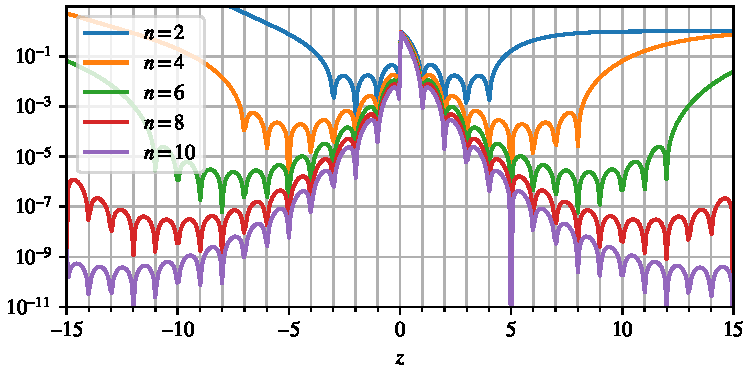
\includegraphics{papers/laguerre/images/rel_error_mirror.pdf}
%\vspace{-12pt}
\caption{Relativer Fehler des Ansatzes mit Spiegelung negativer Realwerte
für verschiedene reele Werte von $z$ und Grade $n$ der Laguerre-Polynome}
\label{laguerre:fig:rel_error_mirror}
\end{figure}

Spiegelt man nun $z$ mit negativem Realteil mittels der Reflektionsformel,
ergibt sich ein stabilerer Fehler in der linken Hälfte,
wie in Abbildung~\ref{laguerre:fig:rel_error_mirror}.
Die Spiegelung bringt nur für wenige Werte einen,
für praktische Anwendungen geeigneten,
relativen Fehler.
Wie wir aber in Abbildung~\ref{laguerre:fig:rel_error_simple} sehen konnten,
gibt es für jeden Polynomgrad $n$ ein Intervall $[a(n), a(n) + 1]$,
$a(n) \in \mathbb{Z}$,
in welchem der relative Fehler minimal ist.
Die Funktionalgleichung der Gamma-Funktion \eqref{laguerre:gamma_funktional}
könnte uns hier helfen,
das Problem in den Griff zu bekommen.

\subsubsection{Analyse des Integranden}
Wie wir im vorherigen Abschnitt gesehen haben,
scheint der Integrand problematisch.
Darum möchten wir jetzt den Integranden analysieren,
um ihn besser verstehen zu können und
dadurch geeignete Gegenmassnahmen zu entwickeln.

% Dieser Abschnitt soll eine grafisches Verständnis dafür schaffen,
% wieso der Integrand so problematisch ist.
% Was das heisst sollte in Abbildung~\ref{laguerre:fig:integrand} 
% und Abbildung~\ref{laguerre:fig:integrand_exp} grafisch dargestellt werden.
\begin{figure}
\centering
% %% Creator: Matplotlib, PGF backend
%%
%% To include the figure in your LaTeX document, write
%%   \input{<filename>.pgf}
%%
%% Make sure the required packages are loaded in your preamble
%%   \usepackage{pgf}
%%
%% Also ensure that all the required font packages are loaded; for instance,
%% the lmodern package is sometimes necessary when using math font.
%%   \usepackage{lmodern}
%%
%% Figures using additional raster images can only be included by \input if
%% they are in the same directory as the main LaTeX file. For loading figures
%% from other directories you can use the `import` package
%%   \usepackage{import}
%%
%% and then include the figures with
%%   \import{<path to file>}{<filename>.pgf}
%%
%% Matplotlib used the following preamble
%%   \usepackage{fontspec}
%%   \setmainfont{DejaVuSerif.ttf}[Path=\detokenize{/home/mup/.local/lib/python3.8/site-packages/matplotlib/mpl-data/fonts/ttf/}]
%%   \setsansfont{DejaVuSans.ttf}[Path=\detokenize{/home/mup/.local/lib/python3.8/site-packages/matplotlib/mpl-data/fonts/ttf/}]
%%   \setmonofont{DejaVuSansMono.ttf}[Path=\detokenize{/home/mup/.local/lib/python3.8/site-packages/matplotlib/mpl-data/fonts/ttf/}]
%%
\begingroup%
\makeatletter%
\begin{pgfpicture}%
\pgfpathrectangle{\pgfpointorigin}{\pgfqpoint{4.000000in}{2.400000in}}%
\pgfusepath{use as bounding box, clip}%
\begin{pgfscope}%
\pgfsetbuttcap%
\pgfsetmiterjoin%
\definecolor{currentfill}{rgb}{1.000000,1.000000,1.000000}%
\pgfsetfillcolor{currentfill}%
\pgfsetlinewidth{0.000000pt}%
\definecolor{currentstroke}{rgb}{1.000000,1.000000,1.000000}%
\pgfsetstrokecolor{currentstroke}%
\pgfsetdash{}{0pt}%
\pgfpathmoveto{\pgfqpoint{0.000000in}{0.000000in}}%
\pgfpathlineto{\pgfqpoint{4.000000in}{0.000000in}}%
\pgfpathlineto{\pgfqpoint{4.000000in}{2.400000in}}%
\pgfpathlineto{\pgfqpoint{0.000000in}{2.400000in}}%
\pgfpathlineto{\pgfqpoint{0.000000in}{0.000000in}}%
\pgfpathclose%
\pgfusepath{fill}%
\end{pgfscope}%
\begin{pgfscope}%
\pgfsetbuttcap%
\pgfsetmiterjoin%
\definecolor{currentfill}{rgb}{1.000000,1.000000,1.000000}%
\pgfsetfillcolor{currentfill}%
\pgfsetlinewidth{0.000000pt}%
\definecolor{currentstroke}{rgb}{0.000000,0.000000,0.000000}%
\pgfsetstrokecolor{currentstroke}%
\pgfsetstrokeopacity{0.000000}%
\pgfsetdash{}{0pt}%
\pgfpathmoveto{\pgfqpoint{0.315623in}{0.463273in}}%
\pgfpathlineto{\pgfqpoint{3.857732in}{0.463273in}}%
\pgfpathlineto{\pgfqpoint{3.857732in}{2.305568in}}%
\pgfpathlineto{\pgfqpoint{0.315623in}{2.305568in}}%
\pgfpathlineto{\pgfqpoint{0.315623in}{0.463273in}}%
\pgfpathclose%
\pgfusepath{fill}%
\end{pgfscope}%
\begin{pgfscope}%
\pgfpathrectangle{\pgfqpoint{0.315623in}{0.463273in}}{\pgfqpoint{3.542109in}{1.842295in}}%
\pgfusepath{clip}%
\pgfsetrectcap%
\pgfsetroundjoin%
\pgfsetlinewidth{0.803000pt}%
\definecolor{currentstroke}{rgb}{0.690196,0.690196,0.690196}%
\pgfsetstrokecolor{currentstroke}%
\pgfsetdash{}{0pt}%
\pgfpathmoveto{\pgfqpoint{0.315623in}{0.463273in}}%
\pgfpathlineto{\pgfqpoint{0.315623in}{2.305568in}}%
\pgfusepath{stroke}%
\end{pgfscope}%
\begin{pgfscope}%
\pgfsetbuttcap%
\pgfsetroundjoin%
\definecolor{currentfill}{rgb}{0.000000,0.000000,0.000000}%
\pgfsetfillcolor{currentfill}%
\pgfsetlinewidth{0.803000pt}%
\definecolor{currentstroke}{rgb}{0.000000,0.000000,0.000000}%
\pgfsetstrokecolor{currentstroke}%
\pgfsetdash{}{0pt}%
\pgfsys@defobject{currentmarker}{\pgfqpoint{0.000000in}{-0.048611in}}{\pgfqpoint{0.000000in}{0.000000in}}{%
\pgfpathmoveto{\pgfqpoint{0.000000in}{0.000000in}}%
\pgfpathlineto{\pgfqpoint{0.000000in}{-0.048611in}}%
\pgfusepath{stroke,fill}%
}%
\begin{pgfscope}%
\pgfsys@transformshift{0.315623in}{0.463273in}%
\pgfsys@useobject{currentmarker}{}%
\end{pgfscope}%
\end{pgfscope}%
\begin{pgfscope}%
\definecolor{textcolor}{rgb}{0.000000,0.000000,0.000000}%
\pgfsetstrokecolor{textcolor}%
\pgfsetfillcolor{textcolor}%
\pgftext[x=0.315623in,y=0.366051in,,top]{\color{textcolor}\sffamily\fontsize{10.000000}{12.000000}\selectfont \(\displaystyle {10^{-3}}\)}%
\end{pgfscope}%
\begin{pgfscope}%
\pgfpathrectangle{\pgfqpoint{0.315623in}{0.463273in}}{\pgfqpoint{3.542109in}{1.842295in}}%
\pgfusepath{clip}%
\pgfsetrectcap%
\pgfsetroundjoin%
\pgfsetlinewidth{0.803000pt}%
\definecolor{currentstroke}{rgb}{0.690196,0.690196,0.690196}%
\pgfsetstrokecolor{currentstroke}%
\pgfsetdash{}{0pt}%
\pgfpathmoveto{\pgfqpoint{0.905974in}{0.463273in}}%
\pgfpathlineto{\pgfqpoint{0.905974in}{2.305568in}}%
\pgfusepath{stroke}%
\end{pgfscope}%
\begin{pgfscope}%
\pgfsetbuttcap%
\pgfsetroundjoin%
\definecolor{currentfill}{rgb}{0.000000,0.000000,0.000000}%
\pgfsetfillcolor{currentfill}%
\pgfsetlinewidth{0.803000pt}%
\definecolor{currentstroke}{rgb}{0.000000,0.000000,0.000000}%
\pgfsetstrokecolor{currentstroke}%
\pgfsetdash{}{0pt}%
\pgfsys@defobject{currentmarker}{\pgfqpoint{0.000000in}{-0.048611in}}{\pgfqpoint{0.000000in}{0.000000in}}{%
\pgfpathmoveto{\pgfqpoint{0.000000in}{0.000000in}}%
\pgfpathlineto{\pgfqpoint{0.000000in}{-0.048611in}}%
\pgfusepath{stroke,fill}%
}%
\begin{pgfscope}%
\pgfsys@transformshift{0.905974in}{0.463273in}%
\pgfsys@useobject{currentmarker}{}%
\end{pgfscope}%
\end{pgfscope}%
\begin{pgfscope}%
\definecolor{textcolor}{rgb}{0.000000,0.000000,0.000000}%
\pgfsetstrokecolor{textcolor}%
\pgfsetfillcolor{textcolor}%
\pgftext[x=0.905974in,y=0.366051in,,top]{\color{textcolor}\sffamily\fontsize{10.000000}{12.000000}\selectfont \(\displaystyle {10^{-2}}\)}%
\end{pgfscope}%
\begin{pgfscope}%
\pgfpathrectangle{\pgfqpoint{0.315623in}{0.463273in}}{\pgfqpoint{3.542109in}{1.842295in}}%
\pgfusepath{clip}%
\pgfsetrectcap%
\pgfsetroundjoin%
\pgfsetlinewidth{0.803000pt}%
\definecolor{currentstroke}{rgb}{0.690196,0.690196,0.690196}%
\pgfsetstrokecolor{currentstroke}%
\pgfsetdash{}{0pt}%
\pgfpathmoveto{\pgfqpoint{1.496326in}{0.463273in}}%
\pgfpathlineto{\pgfqpoint{1.496326in}{2.305568in}}%
\pgfusepath{stroke}%
\end{pgfscope}%
\begin{pgfscope}%
\pgfsetbuttcap%
\pgfsetroundjoin%
\definecolor{currentfill}{rgb}{0.000000,0.000000,0.000000}%
\pgfsetfillcolor{currentfill}%
\pgfsetlinewidth{0.803000pt}%
\definecolor{currentstroke}{rgb}{0.000000,0.000000,0.000000}%
\pgfsetstrokecolor{currentstroke}%
\pgfsetdash{}{0pt}%
\pgfsys@defobject{currentmarker}{\pgfqpoint{0.000000in}{-0.048611in}}{\pgfqpoint{0.000000in}{0.000000in}}{%
\pgfpathmoveto{\pgfqpoint{0.000000in}{0.000000in}}%
\pgfpathlineto{\pgfqpoint{0.000000in}{-0.048611in}}%
\pgfusepath{stroke,fill}%
}%
\begin{pgfscope}%
\pgfsys@transformshift{1.496326in}{0.463273in}%
\pgfsys@useobject{currentmarker}{}%
\end{pgfscope}%
\end{pgfscope}%
\begin{pgfscope}%
\definecolor{textcolor}{rgb}{0.000000,0.000000,0.000000}%
\pgfsetstrokecolor{textcolor}%
\pgfsetfillcolor{textcolor}%
\pgftext[x=1.496326in,y=0.366051in,,top]{\color{textcolor}\sffamily\fontsize{10.000000}{12.000000}\selectfont \(\displaystyle {10^{-1}}\)}%
\end{pgfscope}%
\begin{pgfscope}%
\pgfpathrectangle{\pgfqpoint{0.315623in}{0.463273in}}{\pgfqpoint{3.542109in}{1.842295in}}%
\pgfusepath{clip}%
\pgfsetrectcap%
\pgfsetroundjoin%
\pgfsetlinewidth{0.803000pt}%
\definecolor{currentstroke}{rgb}{0.690196,0.690196,0.690196}%
\pgfsetstrokecolor{currentstroke}%
\pgfsetdash{}{0pt}%
\pgfpathmoveto{\pgfqpoint{2.086677in}{0.463273in}}%
\pgfpathlineto{\pgfqpoint{2.086677in}{2.305568in}}%
\pgfusepath{stroke}%
\end{pgfscope}%
\begin{pgfscope}%
\pgfsetbuttcap%
\pgfsetroundjoin%
\definecolor{currentfill}{rgb}{0.000000,0.000000,0.000000}%
\pgfsetfillcolor{currentfill}%
\pgfsetlinewidth{0.803000pt}%
\definecolor{currentstroke}{rgb}{0.000000,0.000000,0.000000}%
\pgfsetstrokecolor{currentstroke}%
\pgfsetdash{}{0pt}%
\pgfsys@defobject{currentmarker}{\pgfqpoint{0.000000in}{-0.048611in}}{\pgfqpoint{0.000000in}{0.000000in}}{%
\pgfpathmoveto{\pgfqpoint{0.000000in}{0.000000in}}%
\pgfpathlineto{\pgfqpoint{0.000000in}{-0.048611in}}%
\pgfusepath{stroke,fill}%
}%
\begin{pgfscope}%
\pgfsys@transformshift{2.086677in}{0.463273in}%
\pgfsys@useobject{currentmarker}{}%
\end{pgfscope}%
\end{pgfscope}%
\begin{pgfscope}%
\definecolor{textcolor}{rgb}{0.000000,0.000000,0.000000}%
\pgfsetstrokecolor{textcolor}%
\pgfsetfillcolor{textcolor}%
\pgftext[x=2.086677in,y=0.366051in,,top]{\color{textcolor}\sffamily\fontsize{10.000000}{12.000000}\selectfont \(\displaystyle {10^{0}}\)}%
\end{pgfscope}%
\begin{pgfscope}%
\pgfpathrectangle{\pgfqpoint{0.315623in}{0.463273in}}{\pgfqpoint{3.542109in}{1.842295in}}%
\pgfusepath{clip}%
\pgfsetrectcap%
\pgfsetroundjoin%
\pgfsetlinewidth{0.803000pt}%
\definecolor{currentstroke}{rgb}{0.690196,0.690196,0.690196}%
\pgfsetstrokecolor{currentstroke}%
\pgfsetdash{}{0pt}%
\pgfpathmoveto{\pgfqpoint{2.677029in}{0.463273in}}%
\pgfpathlineto{\pgfqpoint{2.677029in}{2.305568in}}%
\pgfusepath{stroke}%
\end{pgfscope}%
\begin{pgfscope}%
\pgfsetbuttcap%
\pgfsetroundjoin%
\definecolor{currentfill}{rgb}{0.000000,0.000000,0.000000}%
\pgfsetfillcolor{currentfill}%
\pgfsetlinewidth{0.803000pt}%
\definecolor{currentstroke}{rgb}{0.000000,0.000000,0.000000}%
\pgfsetstrokecolor{currentstroke}%
\pgfsetdash{}{0pt}%
\pgfsys@defobject{currentmarker}{\pgfqpoint{0.000000in}{-0.048611in}}{\pgfqpoint{0.000000in}{0.000000in}}{%
\pgfpathmoveto{\pgfqpoint{0.000000in}{0.000000in}}%
\pgfpathlineto{\pgfqpoint{0.000000in}{-0.048611in}}%
\pgfusepath{stroke,fill}%
}%
\begin{pgfscope}%
\pgfsys@transformshift{2.677029in}{0.463273in}%
\pgfsys@useobject{currentmarker}{}%
\end{pgfscope}%
\end{pgfscope}%
\begin{pgfscope}%
\definecolor{textcolor}{rgb}{0.000000,0.000000,0.000000}%
\pgfsetstrokecolor{textcolor}%
\pgfsetfillcolor{textcolor}%
\pgftext[x=2.677029in,y=0.366051in,,top]{\color{textcolor}\sffamily\fontsize{10.000000}{12.000000}\selectfont \(\displaystyle {10^{1}}\)}%
\end{pgfscope}%
\begin{pgfscope}%
\pgfpathrectangle{\pgfqpoint{0.315623in}{0.463273in}}{\pgfqpoint{3.542109in}{1.842295in}}%
\pgfusepath{clip}%
\pgfsetrectcap%
\pgfsetroundjoin%
\pgfsetlinewidth{0.803000pt}%
\definecolor{currentstroke}{rgb}{0.690196,0.690196,0.690196}%
\pgfsetstrokecolor{currentstroke}%
\pgfsetdash{}{0pt}%
\pgfpathmoveto{\pgfqpoint{3.267380in}{0.463273in}}%
\pgfpathlineto{\pgfqpoint{3.267380in}{2.305568in}}%
\pgfusepath{stroke}%
\end{pgfscope}%
\begin{pgfscope}%
\pgfsetbuttcap%
\pgfsetroundjoin%
\definecolor{currentfill}{rgb}{0.000000,0.000000,0.000000}%
\pgfsetfillcolor{currentfill}%
\pgfsetlinewidth{0.803000pt}%
\definecolor{currentstroke}{rgb}{0.000000,0.000000,0.000000}%
\pgfsetstrokecolor{currentstroke}%
\pgfsetdash{}{0pt}%
\pgfsys@defobject{currentmarker}{\pgfqpoint{0.000000in}{-0.048611in}}{\pgfqpoint{0.000000in}{0.000000in}}{%
\pgfpathmoveto{\pgfqpoint{0.000000in}{0.000000in}}%
\pgfpathlineto{\pgfqpoint{0.000000in}{-0.048611in}}%
\pgfusepath{stroke,fill}%
}%
\begin{pgfscope}%
\pgfsys@transformshift{3.267380in}{0.463273in}%
\pgfsys@useobject{currentmarker}{}%
\end{pgfscope}%
\end{pgfscope}%
\begin{pgfscope}%
\definecolor{textcolor}{rgb}{0.000000,0.000000,0.000000}%
\pgfsetstrokecolor{textcolor}%
\pgfsetfillcolor{textcolor}%
\pgftext[x=3.267380in,y=0.366051in,,top]{\color{textcolor}\sffamily\fontsize{10.000000}{12.000000}\selectfont \(\displaystyle {10^{2}}\)}%
\end{pgfscope}%
\begin{pgfscope}%
\pgfpathrectangle{\pgfqpoint{0.315623in}{0.463273in}}{\pgfqpoint{3.542109in}{1.842295in}}%
\pgfusepath{clip}%
\pgfsetrectcap%
\pgfsetroundjoin%
\pgfsetlinewidth{0.803000pt}%
\definecolor{currentstroke}{rgb}{0.690196,0.690196,0.690196}%
\pgfsetstrokecolor{currentstroke}%
\pgfsetdash{}{0pt}%
\pgfpathmoveto{\pgfqpoint{3.857732in}{0.463273in}}%
\pgfpathlineto{\pgfqpoint{3.857732in}{2.305568in}}%
\pgfusepath{stroke}%
\end{pgfscope}%
\begin{pgfscope}%
\pgfsetbuttcap%
\pgfsetroundjoin%
\definecolor{currentfill}{rgb}{0.000000,0.000000,0.000000}%
\pgfsetfillcolor{currentfill}%
\pgfsetlinewidth{0.803000pt}%
\definecolor{currentstroke}{rgb}{0.000000,0.000000,0.000000}%
\pgfsetstrokecolor{currentstroke}%
\pgfsetdash{}{0pt}%
\pgfsys@defobject{currentmarker}{\pgfqpoint{0.000000in}{-0.048611in}}{\pgfqpoint{0.000000in}{0.000000in}}{%
\pgfpathmoveto{\pgfqpoint{0.000000in}{0.000000in}}%
\pgfpathlineto{\pgfqpoint{0.000000in}{-0.048611in}}%
\pgfusepath{stroke,fill}%
}%
\begin{pgfscope}%
\pgfsys@transformshift{3.857732in}{0.463273in}%
\pgfsys@useobject{currentmarker}{}%
\end{pgfscope}%
\end{pgfscope}%
\begin{pgfscope}%
\definecolor{textcolor}{rgb}{0.000000,0.000000,0.000000}%
\pgfsetstrokecolor{textcolor}%
\pgfsetfillcolor{textcolor}%
\pgftext[x=3.857732in,y=0.366051in,,top]{\color{textcolor}\sffamily\fontsize{10.000000}{12.000000}\selectfont \(\displaystyle {10^{3}}\)}%
\end{pgfscope}%
\begin{pgfscope}%
\pgfpathrectangle{\pgfqpoint{0.315623in}{0.463273in}}{\pgfqpoint{3.542109in}{1.842295in}}%
\pgfusepath{clip}%
\pgfsetrectcap%
\pgfsetroundjoin%
\pgfsetlinewidth{0.803000pt}%
\definecolor{currentstroke}{rgb}{0.690196,0.690196,0.690196}%
\pgfsetstrokecolor{currentstroke}%
\pgfsetdash{}{0pt}%
\pgfpathmoveto{\pgfqpoint{0.493336in}{0.463273in}}%
\pgfpathlineto{\pgfqpoint{0.493336in}{2.305568in}}%
\pgfusepath{stroke}%
\end{pgfscope}%
\begin{pgfscope}%
\pgfsetbuttcap%
\pgfsetroundjoin%
\definecolor{currentfill}{rgb}{0.000000,0.000000,0.000000}%
\pgfsetfillcolor{currentfill}%
\pgfsetlinewidth{0.602250pt}%
\definecolor{currentstroke}{rgb}{0.000000,0.000000,0.000000}%
\pgfsetstrokecolor{currentstroke}%
\pgfsetdash{}{0pt}%
\pgfsys@defobject{currentmarker}{\pgfqpoint{0.000000in}{-0.027778in}}{\pgfqpoint{0.000000in}{0.000000in}}{%
\pgfpathmoveto{\pgfqpoint{0.000000in}{0.000000in}}%
\pgfpathlineto{\pgfqpoint{0.000000in}{-0.027778in}}%
\pgfusepath{stroke,fill}%
}%
\begin{pgfscope}%
\pgfsys@transformshift{0.493336in}{0.463273in}%
\pgfsys@useobject{currentmarker}{}%
\end{pgfscope}%
\end{pgfscope}%
\begin{pgfscope}%
\pgfpathrectangle{\pgfqpoint{0.315623in}{0.463273in}}{\pgfqpoint{3.542109in}{1.842295in}}%
\pgfusepath{clip}%
\pgfsetrectcap%
\pgfsetroundjoin%
\pgfsetlinewidth{0.803000pt}%
\definecolor{currentstroke}{rgb}{0.690196,0.690196,0.690196}%
\pgfsetstrokecolor{currentstroke}%
\pgfsetdash{}{0pt}%
\pgfpathmoveto{\pgfqpoint{0.597292in}{0.463273in}}%
\pgfpathlineto{\pgfqpoint{0.597292in}{2.305568in}}%
\pgfusepath{stroke}%
\end{pgfscope}%
\begin{pgfscope}%
\pgfsetbuttcap%
\pgfsetroundjoin%
\definecolor{currentfill}{rgb}{0.000000,0.000000,0.000000}%
\pgfsetfillcolor{currentfill}%
\pgfsetlinewidth{0.602250pt}%
\definecolor{currentstroke}{rgb}{0.000000,0.000000,0.000000}%
\pgfsetstrokecolor{currentstroke}%
\pgfsetdash{}{0pt}%
\pgfsys@defobject{currentmarker}{\pgfqpoint{0.000000in}{-0.027778in}}{\pgfqpoint{0.000000in}{0.000000in}}{%
\pgfpathmoveto{\pgfqpoint{0.000000in}{0.000000in}}%
\pgfpathlineto{\pgfqpoint{0.000000in}{-0.027778in}}%
\pgfusepath{stroke,fill}%
}%
\begin{pgfscope}%
\pgfsys@transformshift{0.597292in}{0.463273in}%
\pgfsys@useobject{currentmarker}{}%
\end{pgfscope}%
\end{pgfscope}%
\begin{pgfscope}%
\pgfpathrectangle{\pgfqpoint{0.315623in}{0.463273in}}{\pgfqpoint{3.542109in}{1.842295in}}%
\pgfusepath{clip}%
\pgfsetrectcap%
\pgfsetroundjoin%
\pgfsetlinewidth{0.803000pt}%
\definecolor{currentstroke}{rgb}{0.690196,0.690196,0.690196}%
\pgfsetstrokecolor{currentstroke}%
\pgfsetdash{}{0pt}%
\pgfpathmoveto{\pgfqpoint{0.671050in}{0.463273in}}%
\pgfpathlineto{\pgfqpoint{0.671050in}{2.305568in}}%
\pgfusepath{stroke}%
\end{pgfscope}%
\begin{pgfscope}%
\pgfsetbuttcap%
\pgfsetroundjoin%
\definecolor{currentfill}{rgb}{0.000000,0.000000,0.000000}%
\pgfsetfillcolor{currentfill}%
\pgfsetlinewidth{0.602250pt}%
\definecolor{currentstroke}{rgb}{0.000000,0.000000,0.000000}%
\pgfsetstrokecolor{currentstroke}%
\pgfsetdash{}{0pt}%
\pgfsys@defobject{currentmarker}{\pgfqpoint{0.000000in}{-0.027778in}}{\pgfqpoint{0.000000in}{0.000000in}}{%
\pgfpathmoveto{\pgfqpoint{0.000000in}{0.000000in}}%
\pgfpathlineto{\pgfqpoint{0.000000in}{-0.027778in}}%
\pgfusepath{stroke,fill}%
}%
\begin{pgfscope}%
\pgfsys@transformshift{0.671050in}{0.463273in}%
\pgfsys@useobject{currentmarker}{}%
\end{pgfscope}%
\end{pgfscope}%
\begin{pgfscope}%
\pgfpathrectangle{\pgfqpoint{0.315623in}{0.463273in}}{\pgfqpoint{3.542109in}{1.842295in}}%
\pgfusepath{clip}%
\pgfsetrectcap%
\pgfsetroundjoin%
\pgfsetlinewidth{0.803000pt}%
\definecolor{currentstroke}{rgb}{0.690196,0.690196,0.690196}%
\pgfsetstrokecolor{currentstroke}%
\pgfsetdash{}{0pt}%
\pgfpathmoveto{\pgfqpoint{0.728261in}{0.463273in}}%
\pgfpathlineto{\pgfqpoint{0.728261in}{2.305568in}}%
\pgfusepath{stroke}%
\end{pgfscope}%
\begin{pgfscope}%
\pgfsetbuttcap%
\pgfsetroundjoin%
\definecolor{currentfill}{rgb}{0.000000,0.000000,0.000000}%
\pgfsetfillcolor{currentfill}%
\pgfsetlinewidth{0.602250pt}%
\definecolor{currentstroke}{rgb}{0.000000,0.000000,0.000000}%
\pgfsetstrokecolor{currentstroke}%
\pgfsetdash{}{0pt}%
\pgfsys@defobject{currentmarker}{\pgfqpoint{0.000000in}{-0.027778in}}{\pgfqpoint{0.000000in}{0.000000in}}{%
\pgfpathmoveto{\pgfqpoint{0.000000in}{0.000000in}}%
\pgfpathlineto{\pgfqpoint{0.000000in}{-0.027778in}}%
\pgfusepath{stroke,fill}%
}%
\begin{pgfscope}%
\pgfsys@transformshift{0.728261in}{0.463273in}%
\pgfsys@useobject{currentmarker}{}%
\end{pgfscope}%
\end{pgfscope}%
\begin{pgfscope}%
\pgfpathrectangle{\pgfqpoint{0.315623in}{0.463273in}}{\pgfqpoint{3.542109in}{1.842295in}}%
\pgfusepath{clip}%
\pgfsetrectcap%
\pgfsetroundjoin%
\pgfsetlinewidth{0.803000pt}%
\definecolor{currentstroke}{rgb}{0.690196,0.690196,0.690196}%
\pgfsetstrokecolor{currentstroke}%
\pgfsetdash{}{0pt}%
\pgfpathmoveto{\pgfqpoint{0.775006in}{0.463273in}}%
\pgfpathlineto{\pgfqpoint{0.775006in}{2.305568in}}%
\pgfusepath{stroke}%
\end{pgfscope}%
\begin{pgfscope}%
\pgfsetbuttcap%
\pgfsetroundjoin%
\definecolor{currentfill}{rgb}{0.000000,0.000000,0.000000}%
\pgfsetfillcolor{currentfill}%
\pgfsetlinewidth{0.602250pt}%
\definecolor{currentstroke}{rgb}{0.000000,0.000000,0.000000}%
\pgfsetstrokecolor{currentstroke}%
\pgfsetdash{}{0pt}%
\pgfsys@defobject{currentmarker}{\pgfqpoint{0.000000in}{-0.027778in}}{\pgfqpoint{0.000000in}{0.000000in}}{%
\pgfpathmoveto{\pgfqpoint{0.000000in}{0.000000in}}%
\pgfpathlineto{\pgfqpoint{0.000000in}{-0.027778in}}%
\pgfusepath{stroke,fill}%
}%
\begin{pgfscope}%
\pgfsys@transformshift{0.775006in}{0.463273in}%
\pgfsys@useobject{currentmarker}{}%
\end{pgfscope}%
\end{pgfscope}%
\begin{pgfscope}%
\pgfpathrectangle{\pgfqpoint{0.315623in}{0.463273in}}{\pgfqpoint{3.542109in}{1.842295in}}%
\pgfusepath{clip}%
\pgfsetrectcap%
\pgfsetroundjoin%
\pgfsetlinewidth{0.803000pt}%
\definecolor{currentstroke}{rgb}{0.690196,0.690196,0.690196}%
\pgfsetstrokecolor{currentstroke}%
\pgfsetdash{}{0pt}%
\pgfpathmoveto{\pgfqpoint{0.814528in}{0.463273in}}%
\pgfpathlineto{\pgfqpoint{0.814528in}{2.305568in}}%
\pgfusepath{stroke}%
\end{pgfscope}%
\begin{pgfscope}%
\pgfsetbuttcap%
\pgfsetroundjoin%
\definecolor{currentfill}{rgb}{0.000000,0.000000,0.000000}%
\pgfsetfillcolor{currentfill}%
\pgfsetlinewidth{0.602250pt}%
\definecolor{currentstroke}{rgb}{0.000000,0.000000,0.000000}%
\pgfsetstrokecolor{currentstroke}%
\pgfsetdash{}{0pt}%
\pgfsys@defobject{currentmarker}{\pgfqpoint{0.000000in}{-0.027778in}}{\pgfqpoint{0.000000in}{0.000000in}}{%
\pgfpathmoveto{\pgfqpoint{0.000000in}{0.000000in}}%
\pgfpathlineto{\pgfqpoint{0.000000in}{-0.027778in}}%
\pgfusepath{stroke,fill}%
}%
\begin{pgfscope}%
\pgfsys@transformshift{0.814528in}{0.463273in}%
\pgfsys@useobject{currentmarker}{}%
\end{pgfscope}%
\end{pgfscope}%
\begin{pgfscope}%
\pgfpathrectangle{\pgfqpoint{0.315623in}{0.463273in}}{\pgfqpoint{3.542109in}{1.842295in}}%
\pgfusepath{clip}%
\pgfsetrectcap%
\pgfsetroundjoin%
\pgfsetlinewidth{0.803000pt}%
\definecolor{currentstroke}{rgb}{0.690196,0.690196,0.690196}%
\pgfsetstrokecolor{currentstroke}%
\pgfsetdash{}{0pt}%
\pgfpathmoveto{\pgfqpoint{0.848763in}{0.463273in}}%
\pgfpathlineto{\pgfqpoint{0.848763in}{2.305568in}}%
\pgfusepath{stroke}%
\end{pgfscope}%
\begin{pgfscope}%
\pgfsetbuttcap%
\pgfsetroundjoin%
\definecolor{currentfill}{rgb}{0.000000,0.000000,0.000000}%
\pgfsetfillcolor{currentfill}%
\pgfsetlinewidth{0.602250pt}%
\definecolor{currentstroke}{rgb}{0.000000,0.000000,0.000000}%
\pgfsetstrokecolor{currentstroke}%
\pgfsetdash{}{0pt}%
\pgfsys@defobject{currentmarker}{\pgfqpoint{0.000000in}{-0.027778in}}{\pgfqpoint{0.000000in}{0.000000in}}{%
\pgfpathmoveto{\pgfqpoint{0.000000in}{0.000000in}}%
\pgfpathlineto{\pgfqpoint{0.000000in}{-0.027778in}}%
\pgfusepath{stroke,fill}%
}%
\begin{pgfscope}%
\pgfsys@transformshift{0.848763in}{0.463273in}%
\pgfsys@useobject{currentmarker}{}%
\end{pgfscope}%
\end{pgfscope}%
\begin{pgfscope}%
\pgfpathrectangle{\pgfqpoint{0.315623in}{0.463273in}}{\pgfqpoint{3.542109in}{1.842295in}}%
\pgfusepath{clip}%
\pgfsetrectcap%
\pgfsetroundjoin%
\pgfsetlinewidth{0.803000pt}%
\definecolor{currentstroke}{rgb}{0.690196,0.690196,0.690196}%
\pgfsetstrokecolor{currentstroke}%
\pgfsetdash{}{0pt}%
\pgfpathmoveto{\pgfqpoint{0.878961in}{0.463273in}}%
\pgfpathlineto{\pgfqpoint{0.878961in}{2.305568in}}%
\pgfusepath{stroke}%
\end{pgfscope}%
\begin{pgfscope}%
\pgfsetbuttcap%
\pgfsetroundjoin%
\definecolor{currentfill}{rgb}{0.000000,0.000000,0.000000}%
\pgfsetfillcolor{currentfill}%
\pgfsetlinewidth{0.602250pt}%
\definecolor{currentstroke}{rgb}{0.000000,0.000000,0.000000}%
\pgfsetstrokecolor{currentstroke}%
\pgfsetdash{}{0pt}%
\pgfsys@defobject{currentmarker}{\pgfqpoint{0.000000in}{-0.027778in}}{\pgfqpoint{0.000000in}{0.000000in}}{%
\pgfpathmoveto{\pgfqpoint{0.000000in}{0.000000in}}%
\pgfpathlineto{\pgfqpoint{0.000000in}{-0.027778in}}%
\pgfusepath{stroke,fill}%
}%
\begin{pgfscope}%
\pgfsys@transformshift{0.878961in}{0.463273in}%
\pgfsys@useobject{currentmarker}{}%
\end{pgfscope}%
\end{pgfscope}%
\begin{pgfscope}%
\pgfpathrectangle{\pgfqpoint{0.315623in}{0.463273in}}{\pgfqpoint{3.542109in}{1.842295in}}%
\pgfusepath{clip}%
\pgfsetrectcap%
\pgfsetroundjoin%
\pgfsetlinewidth{0.803000pt}%
\definecolor{currentstroke}{rgb}{0.690196,0.690196,0.690196}%
\pgfsetstrokecolor{currentstroke}%
\pgfsetdash{}{0pt}%
\pgfpathmoveto{\pgfqpoint{1.083688in}{0.463273in}}%
\pgfpathlineto{\pgfqpoint{1.083688in}{2.305568in}}%
\pgfusepath{stroke}%
\end{pgfscope}%
\begin{pgfscope}%
\pgfsetbuttcap%
\pgfsetroundjoin%
\definecolor{currentfill}{rgb}{0.000000,0.000000,0.000000}%
\pgfsetfillcolor{currentfill}%
\pgfsetlinewidth{0.602250pt}%
\definecolor{currentstroke}{rgb}{0.000000,0.000000,0.000000}%
\pgfsetstrokecolor{currentstroke}%
\pgfsetdash{}{0pt}%
\pgfsys@defobject{currentmarker}{\pgfqpoint{0.000000in}{-0.027778in}}{\pgfqpoint{0.000000in}{0.000000in}}{%
\pgfpathmoveto{\pgfqpoint{0.000000in}{0.000000in}}%
\pgfpathlineto{\pgfqpoint{0.000000in}{-0.027778in}}%
\pgfusepath{stroke,fill}%
}%
\begin{pgfscope}%
\pgfsys@transformshift{1.083688in}{0.463273in}%
\pgfsys@useobject{currentmarker}{}%
\end{pgfscope}%
\end{pgfscope}%
\begin{pgfscope}%
\pgfpathrectangle{\pgfqpoint{0.315623in}{0.463273in}}{\pgfqpoint{3.542109in}{1.842295in}}%
\pgfusepath{clip}%
\pgfsetrectcap%
\pgfsetroundjoin%
\pgfsetlinewidth{0.803000pt}%
\definecolor{currentstroke}{rgb}{0.690196,0.690196,0.690196}%
\pgfsetstrokecolor{currentstroke}%
\pgfsetdash{}{0pt}%
\pgfpathmoveto{\pgfqpoint{1.187644in}{0.463273in}}%
\pgfpathlineto{\pgfqpoint{1.187644in}{2.305568in}}%
\pgfusepath{stroke}%
\end{pgfscope}%
\begin{pgfscope}%
\pgfsetbuttcap%
\pgfsetroundjoin%
\definecolor{currentfill}{rgb}{0.000000,0.000000,0.000000}%
\pgfsetfillcolor{currentfill}%
\pgfsetlinewidth{0.602250pt}%
\definecolor{currentstroke}{rgb}{0.000000,0.000000,0.000000}%
\pgfsetstrokecolor{currentstroke}%
\pgfsetdash{}{0pt}%
\pgfsys@defobject{currentmarker}{\pgfqpoint{0.000000in}{-0.027778in}}{\pgfqpoint{0.000000in}{0.000000in}}{%
\pgfpathmoveto{\pgfqpoint{0.000000in}{0.000000in}}%
\pgfpathlineto{\pgfqpoint{0.000000in}{-0.027778in}}%
\pgfusepath{stroke,fill}%
}%
\begin{pgfscope}%
\pgfsys@transformshift{1.187644in}{0.463273in}%
\pgfsys@useobject{currentmarker}{}%
\end{pgfscope}%
\end{pgfscope}%
\begin{pgfscope}%
\pgfpathrectangle{\pgfqpoint{0.315623in}{0.463273in}}{\pgfqpoint{3.542109in}{1.842295in}}%
\pgfusepath{clip}%
\pgfsetrectcap%
\pgfsetroundjoin%
\pgfsetlinewidth{0.803000pt}%
\definecolor{currentstroke}{rgb}{0.690196,0.690196,0.690196}%
\pgfsetstrokecolor{currentstroke}%
\pgfsetdash{}{0pt}%
\pgfpathmoveto{\pgfqpoint{1.261401in}{0.463273in}}%
\pgfpathlineto{\pgfqpoint{1.261401in}{2.305568in}}%
\pgfusepath{stroke}%
\end{pgfscope}%
\begin{pgfscope}%
\pgfsetbuttcap%
\pgfsetroundjoin%
\definecolor{currentfill}{rgb}{0.000000,0.000000,0.000000}%
\pgfsetfillcolor{currentfill}%
\pgfsetlinewidth{0.602250pt}%
\definecolor{currentstroke}{rgb}{0.000000,0.000000,0.000000}%
\pgfsetstrokecolor{currentstroke}%
\pgfsetdash{}{0pt}%
\pgfsys@defobject{currentmarker}{\pgfqpoint{0.000000in}{-0.027778in}}{\pgfqpoint{0.000000in}{0.000000in}}{%
\pgfpathmoveto{\pgfqpoint{0.000000in}{0.000000in}}%
\pgfpathlineto{\pgfqpoint{0.000000in}{-0.027778in}}%
\pgfusepath{stroke,fill}%
}%
\begin{pgfscope}%
\pgfsys@transformshift{1.261401in}{0.463273in}%
\pgfsys@useobject{currentmarker}{}%
\end{pgfscope}%
\end{pgfscope}%
\begin{pgfscope}%
\pgfpathrectangle{\pgfqpoint{0.315623in}{0.463273in}}{\pgfqpoint{3.542109in}{1.842295in}}%
\pgfusepath{clip}%
\pgfsetrectcap%
\pgfsetroundjoin%
\pgfsetlinewidth{0.803000pt}%
\definecolor{currentstroke}{rgb}{0.690196,0.690196,0.690196}%
\pgfsetstrokecolor{currentstroke}%
\pgfsetdash{}{0pt}%
\pgfpathmoveto{\pgfqpoint{1.318612in}{0.463273in}}%
\pgfpathlineto{\pgfqpoint{1.318612in}{2.305568in}}%
\pgfusepath{stroke}%
\end{pgfscope}%
\begin{pgfscope}%
\pgfsetbuttcap%
\pgfsetroundjoin%
\definecolor{currentfill}{rgb}{0.000000,0.000000,0.000000}%
\pgfsetfillcolor{currentfill}%
\pgfsetlinewidth{0.602250pt}%
\definecolor{currentstroke}{rgb}{0.000000,0.000000,0.000000}%
\pgfsetstrokecolor{currentstroke}%
\pgfsetdash{}{0pt}%
\pgfsys@defobject{currentmarker}{\pgfqpoint{0.000000in}{-0.027778in}}{\pgfqpoint{0.000000in}{0.000000in}}{%
\pgfpathmoveto{\pgfqpoint{0.000000in}{0.000000in}}%
\pgfpathlineto{\pgfqpoint{0.000000in}{-0.027778in}}%
\pgfusepath{stroke,fill}%
}%
\begin{pgfscope}%
\pgfsys@transformshift{1.318612in}{0.463273in}%
\pgfsys@useobject{currentmarker}{}%
\end{pgfscope}%
\end{pgfscope}%
\begin{pgfscope}%
\pgfpathrectangle{\pgfqpoint{0.315623in}{0.463273in}}{\pgfqpoint{3.542109in}{1.842295in}}%
\pgfusepath{clip}%
\pgfsetrectcap%
\pgfsetroundjoin%
\pgfsetlinewidth{0.803000pt}%
\definecolor{currentstroke}{rgb}{0.690196,0.690196,0.690196}%
\pgfsetstrokecolor{currentstroke}%
\pgfsetdash{}{0pt}%
\pgfpathmoveto{\pgfqpoint{1.365357in}{0.463273in}}%
\pgfpathlineto{\pgfqpoint{1.365357in}{2.305568in}}%
\pgfusepath{stroke}%
\end{pgfscope}%
\begin{pgfscope}%
\pgfsetbuttcap%
\pgfsetroundjoin%
\definecolor{currentfill}{rgb}{0.000000,0.000000,0.000000}%
\pgfsetfillcolor{currentfill}%
\pgfsetlinewidth{0.602250pt}%
\definecolor{currentstroke}{rgb}{0.000000,0.000000,0.000000}%
\pgfsetstrokecolor{currentstroke}%
\pgfsetdash{}{0pt}%
\pgfsys@defobject{currentmarker}{\pgfqpoint{0.000000in}{-0.027778in}}{\pgfqpoint{0.000000in}{0.000000in}}{%
\pgfpathmoveto{\pgfqpoint{0.000000in}{0.000000in}}%
\pgfpathlineto{\pgfqpoint{0.000000in}{-0.027778in}}%
\pgfusepath{stroke,fill}%
}%
\begin{pgfscope}%
\pgfsys@transformshift{1.365357in}{0.463273in}%
\pgfsys@useobject{currentmarker}{}%
\end{pgfscope}%
\end{pgfscope}%
\begin{pgfscope}%
\pgfpathrectangle{\pgfqpoint{0.315623in}{0.463273in}}{\pgfqpoint{3.542109in}{1.842295in}}%
\pgfusepath{clip}%
\pgfsetrectcap%
\pgfsetroundjoin%
\pgfsetlinewidth{0.803000pt}%
\definecolor{currentstroke}{rgb}{0.690196,0.690196,0.690196}%
\pgfsetstrokecolor{currentstroke}%
\pgfsetdash{}{0pt}%
\pgfpathmoveto{\pgfqpoint{1.404879in}{0.463273in}}%
\pgfpathlineto{\pgfqpoint{1.404879in}{2.305568in}}%
\pgfusepath{stroke}%
\end{pgfscope}%
\begin{pgfscope}%
\pgfsetbuttcap%
\pgfsetroundjoin%
\definecolor{currentfill}{rgb}{0.000000,0.000000,0.000000}%
\pgfsetfillcolor{currentfill}%
\pgfsetlinewidth{0.602250pt}%
\definecolor{currentstroke}{rgb}{0.000000,0.000000,0.000000}%
\pgfsetstrokecolor{currentstroke}%
\pgfsetdash{}{0pt}%
\pgfsys@defobject{currentmarker}{\pgfqpoint{0.000000in}{-0.027778in}}{\pgfqpoint{0.000000in}{0.000000in}}{%
\pgfpathmoveto{\pgfqpoint{0.000000in}{0.000000in}}%
\pgfpathlineto{\pgfqpoint{0.000000in}{-0.027778in}}%
\pgfusepath{stroke,fill}%
}%
\begin{pgfscope}%
\pgfsys@transformshift{1.404879in}{0.463273in}%
\pgfsys@useobject{currentmarker}{}%
\end{pgfscope}%
\end{pgfscope}%
\begin{pgfscope}%
\pgfpathrectangle{\pgfqpoint{0.315623in}{0.463273in}}{\pgfqpoint{3.542109in}{1.842295in}}%
\pgfusepath{clip}%
\pgfsetrectcap%
\pgfsetroundjoin%
\pgfsetlinewidth{0.803000pt}%
\definecolor{currentstroke}{rgb}{0.690196,0.690196,0.690196}%
\pgfsetstrokecolor{currentstroke}%
\pgfsetdash{}{0pt}%
\pgfpathmoveto{\pgfqpoint{1.439115in}{0.463273in}}%
\pgfpathlineto{\pgfqpoint{1.439115in}{2.305568in}}%
\pgfusepath{stroke}%
\end{pgfscope}%
\begin{pgfscope}%
\pgfsetbuttcap%
\pgfsetroundjoin%
\definecolor{currentfill}{rgb}{0.000000,0.000000,0.000000}%
\pgfsetfillcolor{currentfill}%
\pgfsetlinewidth{0.602250pt}%
\definecolor{currentstroke}{rgb}{0.000000,0.000000,0.000000}%
\pgfsetstrokecolor{currentstroke}%
\pgfsetdash{}{0pt}%
\pgfsys@defobject{currentmarker}{\pgfqpoint{0.000000in}{-0.027778in}}{\pgfqpoint{0.000000in}{0.000000in}}{%
\pgfpathmoveto{\pgfqpoint{0.000000in}{0.000000in}}%
\pgfpathlineto{\pgfqpoint{0.000000in}{-0.027778in}}%
\pgfusepath{stroke,fill}%
}%
\begin{pgfscope}%
\pgfsys@transformshift{1.439115in}{0.463273in}%
\pgfsys@useobject{currentmarker}{}%
\end{pgfscope}%
\end{pgfscope}%
\begin{pgfscope}%
\pgfpathrectangle{\pgfqpoint{0.315623in}{0.463273in}}{\pgfqpoint{3.542109in}{1.842295in}}%
\pgfusepath{clip}%
\pgfsetrectcap%
\pgfsetroundjoin%
\pgfsetlinewidth{0.803000pt}%
\definecolor{currentstroke}{rgb}{0.690196,0.690196,0.690196}%
\pgfsetstrokecolor{currentstroke}%
\pgfsetdash{}{0pt}%
\pgfpathmoveto{\pgfqpoint{1.469313in}{0.463273in}}%
\pgfpathlineto{\pgfqpoint{1.469313in}{2.305568in}}%
\pgfusepath{stroke}%
\end{pgfscope}%
\begin{pgfscope}%
\pgfsetbuttcap%
\pgfsetroundjoin%
\definecolor{currentfill}{rgb}{0.000000,0.000000,0.000000}%
\pgfsetfillcolor{currentfill}%
\pgfsetlinewidth{0.602250pt}%
\definecolor{currentstroke}{rgb}{0.000000,0.000000,0.000000}%
\pgfsetstrokecolor{currentstroke}%
\pgfsetdash{}{0pt}%
\pgfsys@defobject{currentmarker}{\pgfqpoint{0.000000in}{-0.027778in}}{\pgfqpoint{0.000000in}{0.000000in}}{%
\pgfpathmoveto{\pgfqpoint{0.000000in}{0.000000in}}%
\pgfpathlineto{\pgfqpoint{0.000000in}{-0.027778in}}%
\pgfusepath{stroke,fill}%
}%
\begin{pgfscope}%
\pgfsys@transformshift{1.469313in}{0.463273in}%
\pgfsys@useobject{currentmarker}{}%
\end{pgfscope}%
\end{pgfscope}%
\begin{pgfscope}%
\pgfpathrectangle{\pgfqpoint{0.315623in}{0.463273in}}{\pgfqpoint{3.542109in}{1.842295in}}%
\pgfusepath{clip}%
\pgfsetrectcap%
\pgfsetroundjoin%
\pgfsetlinewidth{0.803000pt}%
\definecolor{currentstroke}{rgb}{0.690196,0.690196,0.690196}%
\pgfsetstrokecolor{currentstroke}%
\pgfsetdash{}{0pt}%
\pgfpathmoveto{\pgfqpoint{1.674039in}{0.463273in}}%
\pgfpathlineto{\pgfqpoint{1.674039in}{2.305568in}}%
\pgfusepath{stroke}%
\end{pgfscope}%
\begin{pgfscope}%
\pgfsetbuttcap%
\pgfsetroundjoin%
\definecolor{currentfill}{rgb}{0.000000,0.000000,0.000000}%
\pgfsetfillcolor{currentfill}%
\pgfsetlinewidth{0.602250pt}%
\definecolor{currentstroke}{rgb}{0.000000,0.000000,0.000000}%
\pgfsetstrokecolor{currentstroke}%
\pgfsetdash{}{0pt}%
\pgfsys@defobject{currentmarker}{\pgfqpoint{0.000000in}{-0.027778in}}{\pgfqpoint{0.000000in}{0.000000in}}{%
\pgfpathmoveto{\pgfqpoint{0.000000in}{0.000000in}}%
\pgfpathlineto{\pgfqpoint{0.000000in}{-0.027778in}}%
\pgfusepath{stroke,fill}%
}%
\begin{pgfscope}%
\pgfsys@transformshift{1.674039in}{0.463273in}%
\pgfsys@useobject{currentmarker}{}%
\end{pgfscope}%
\end{pgfscope}%
\begin{pgfscope}%
\pgfpathrectangle{\pgfqpoint{0.315623in}{0.463273in}}{\pgfqpoint{3.542109in}{1.842295in}}%
\pgfusepath{clip}%
\pgfsetrectcap%
\pgfsetroundjoin%
\pgfsetlinewidth{0.803000pt}%
\definecolor{currentstroke}{rgb}{0.690196,0.690196,0.690196}%
\pgfsetstrokecolor{currentstroke}%
\pgfsetdash{}{0pt}%
\pgfpathmoveto{\pgfqpoint{1.777995in}{0.463273in}}%
\pgfpathlineto{\pgfqpoint{1.777995in}{2.305568in}}%
\pgfusepath{stroke}%
\end{pgfscope}%
\begin{pgfscope}%
\pgfsetbuttcap%
\pgfsetroundjoin%
\definecolor{currentfill}{rgb}{0.000000,0.000000,0.000000}%
\pgfsetfillcolor{currentfill}%
\pgfsetlinewidth{0.602250pt}%
\definecolor{currentstroke}{rgb}{0.000000,0.000000,0.000000}%
\pgfsetstrokecolor{currentstroke}%
\pgfsetdash{}{0pt}%
\pgfsys@defobject{currentmarker}{\pgfqpoint{0.000000in}{-0.027778in}}{\pgfqpoint{0.000000in}{0.000000in}}{%
\pgfpathmoveto{\pgfqpoint{0.000000in}{0.000000in}}%
\pgfpathlineto{\pgfqpoint{0.000000in}{-0.027778in}}%
\pgfusepath{stroke,fill}%
}%
\begin{pgfscope}%
\pgfsys@transformshift{1.777995in}{0.463273in}%
\pgfsys@useobject{currentmarker}{}%
\end{pgfscope}%
\end{pgfscope}%
\begin{pgfscope}%
\pgfpathrectangle{\pgfqpoint{0.315623in}{0.463273in}}{\pgfqpoint{3.542109in}{1.842295in}}%
\pgfusepath{clip}%
\pgfsetrectcap%
\pgfsetroundjoin%
\pgfsetlinewidth{0.803000pt}%
\definecolor{currentstroke}{rgb}{0.690196,0.690196,0.690196}%
\pgfsetstrokecolor{currentstroke}%
\pgfsetdash{}{0pt}%
\pgfpathmoveto{\pgfqpoint{1.851753in}{0.463273in}}%
\pgfpathlineto{\pgfqpoint{1.851753in}{2.305568in}}%
\pgfusepath{stroke}%
\end{pgfscope}%
\begin{pgfscope}%
\pgfsetbuttcap%
\pgfsetroundjoin%
\definecolor{currentfill}{rgb}{0.000000,0.000000,0.000000}%
\pgfsetfillcolor{currentfill}%
\pgfsetlinewidth{0.602250pt}%
\definecolor{currentstroke}{rgb}{0.000000,0.000000,0.000000}%
\pgfsetstrokecolor{currentstroke}%
\pgfsetdash{}{0pt}%
\pgfsys@defobject{currentmarker}{\pgfqpoint{0.000000in}{-0.027778in}}{\pgfqpoint{0.000000in}{0.000000in}}{%
\pgfpathmoveto{\pgfqpoint{0.000000in}{0.000000in}}%
\pgfpathlineto{\pgfqpoint{0.000000in}{-0.027778in}}%
\pgfusepath{stroke,fill}%
}%
\begin{pgfscope}%
\pgfsys@transformshift{1.851753in}{0.463273in}%
\pgfsys@useobject{currentmarker}{}%
\end{pgfscope}%
\end{pgfscope}%
\begin{pgfscope}%
\pgfpathrectangle{\pgfqpoint{0.315623in}{0.463273in}}{\pgfqpoint{3.542109in}{1.842295in}}%
\pgfusepath{clip}%
\pgfsetrectcap%
\pgfsetroundjoin%
\pgfsetlinewidth{0.803000pt}%
\definecolor{currentstroke}{rgb}{0.690196,0.690196,0.690196}%
\pgfsetstrokecolor{currentstroke}%
\pgfsetdash{}{0pt}%
\pgfpathmoveto{\pgfqpoint{1.908964in}{0.463273in}}%
\pgfpathlineto{\pgfqpoint{1.908964in}{2.305568in}}%
\pgfusepath{stroke}%
\end{pgfscope}%
\begin{pgfscope}%
\pgfsetbuttcap%
\pgfsetroundjoin%
\definecolor{currentfill}{rgb}{0.000000,0.000000,0.000000}%
\pgfsetfillcolor{currentfill}%
\pgfsetlinewidth{0.602250pt}%
\definecolor{currentstroke}{rgb}{0.000000,0.000000,0.000000}%
\pgfsetstrokecolor{currentstroke}%
\pgfsetdash{}{0pt}%
\pgfsys@defobject{currentmarker}{\pgfqpoint{0.000000in}{-0.027778in}}{\pgfqpoint{0.000000in}{0.000000in}}{%
\pgfpathmoveto{\pgfqpoint{0.000000in}{0.000000in}}%
\pgfpathlineto{\pgfqpoint{0.000000in}{-0.027778in}}%
\pgfusepath{stroke,fill}%
}%
\begin{pgfscope}%
\pgfsys@transformshift{1.908964in}{0.463273in}%
\pgfsys@useobject{currentmarker}{}%
\end{pgfscope}%
\end{pgfscope}%
\begin{pgfscope}%
\pgfpathrectangle{\pgfqpoint{0.315623in}{0.463273in}}{\pgfqpoint{3.542109in}{1.842295in}}%
\pgfusepath{clip}%
\pgfsetrectcap%
\pgfsetroundjoin%
\pgfsetlinewidth{0.803000pt}%
\definecolor{currentstroke}{rgb}{0.690196,0.690196,0.690196}%
\pgfsetstrokecolor{currentstroke}%
\pgfsetdash{}{0pt}%
\pgfpathmoveto{\pgfqpoint{1.955709in}{0.463273in}}%
\pgfpathlineto{\pgfqpoint{1.955709in}{2.305568in}}%
\pgfusepath{stroke}%
\end{pgfscope}%
\begin{pgfscope}%
\pgfsetbuttcap%
\pgfsetroundjoin%
\definecolor{currentfill}{rgb}{0.000000,0.000000,0.000000}%
\pgfsetfillcolor{currentfill}%
\pgfsetlinewidth{0.602250pt}%
\definecolor{currentstroke}{rgb}{0.000000,0.000000,0.000000}%
\pgfsetstrokecolor{currentstroke}%
\pgfsetdash{}{0pt}%
\pgfsys@defobject{currentmarker}{\pgfqpoint{0.000000in}{-0.027778in}}{\pgfqpoint{0.000000in}{0.000000in}}{%
\pgfpathmoveto{\pgfqpoint{0.000000in}{0.000000in}}%
\pgfpathlineto{\pgfqpoint{0.000000in}{-0.027778in}}%
\pgfusepath{stroke,fill}%
}%
\begin{pgfscope}%
\pgfsys@transformshift{1.955709in}{0.463273in}%
\pgfsys@useobject{currentmarker}{}%
\end{pgfscope}%
\end{pgfscope}%
\begin{pgfscope}%
\pgfpathrectangle{\pgfqpoint{0.315623in}{0.463273in}}{\pgfqpoint{3.542109in}{1.842295in}}%
\pgfusepath{clip}%
\pgfsetrectcap%
\pgfsetroundjoin%
\pgfsetlinewidth{0.803000pt}%
\definecolor{currentstroke}{rgb}{0.690196,0.690196,0.690196}%
\pgfsetstrokecolor{currentstroke}%
\pgfsetdash{}{0pt}%
\pgfpathmoveto{\pgfqpoint{1.995231in}{0.463273in}}%
\pgfpathlineto{\pgfqpoint{1.995231in}{2.305568in}}%
\pgfusepath{stroke}%
\end{pgfscope}%
\begin{pgfscope}%
\pgfsetbuttcap%
\pgfsetroundjoin%
\definecolor{currentfill}{rgb}{0.000000,0.000000,0.000000}%
\pgfsetfillcolor{currentfill}%
\pgfsetlinewidth{0.602250pt}%
\definecolor{currentstroke}{rgb}{0.000000,0.000000,0.000000}%
\pgfsetstrokecolor{currentstroke}%
\pgfsetdash{}{0pt}%
\pgfsys@defobject{currentmarker}{\pgfqpoint{0.000000in}{-0.027778in}}{\pgfqpoint{0.000000in}{0.000000in}}{%
\pgfpathmoveto{\pgfqpoint{0.000000in}{0.000000in}}%
\pgfpathlineto{\pgfqpoint{0.000000in}{-0.027778in}}%
\pgfusepath{stroke,fill}%
}%
\begin{pgfscope}%
\pgfsys@transformshift{1.995231in}{0.463273in}%
\pgfsys@useobject{currentmarker}{}%
\end{pgfscope}%
\end{pgfscope}%
\begin{pgfscope}%
\pgfpathrectangle{\pgfqpoint{0.315623in}{0.463273in}}{\pgfqpoint{3.542109in}{1.842295in}}%
\pgfusepath{clip}%
\pgfsetrectcap%
\pgfsetroundjoin%
\pgfsetlinewidth{0.803000pt}%
\definecolor{currentstroke}{rgb}{0.690196,0.690196,0.690196}%
\pgfsetstrokecolor{currentstroke}%
\pgfsetdash{}{0pt}%
\pgfpathmoveto{\pgfqpoint{2.029466in}{0.463273in}}%
\pgfpathlineto{\pgfqpoint{2.029466in}{2.305568in}}%
\pgfusepath{stroke}%
\end{pgfscope}%
\begin{pgfscope}%
\pgfsetbuttcap%
\pgfsetroundjoin%
\definecolor{currentfill}{rgb}{0.000000,0.000000,0.000000}%
\pgfsetfillcolor{currentfill}%
\pgfsetlinewidth{0.602250pt}%
\definecolor{currentstroke}{rgb}{0.000000,0.000000,0.000000}%
\pgfsetstrokecolor{currentstroke}%
\pgfsetdash{}{0pt}%
\pgfsys@defobject{currentmarker}{\pgfqpoint{0.000000in}{-0.027778in}}{\pgfqpoint{0.000000in}{0.000000in}}{%
\pgfpathmoveto{\pgfqpoint{0.000000in}{0.000000in}}%
\pgfpathlineto{\pgfqpoint{0.000000in}{-0.027778in}}%
\pgfusepath{stroke,fill}%
}%
\begin{pgfscope}%
\pgfsys@transformshift{2.029466in}{0.463273in}%
\pgfsys@useobject{currentmarker}{}%
\end{pgfscope}%
\end{pgfscope}%
\begin{pgfscope}%
\pgfpathrectangle{\pgfqpoint{0.315623in}{0.463273in}}{\pgfqpoint{3.542109in}{1.842295in}}%
\pgfusepath{clip}%
\pgfsetrectcap%
\pgfsetroundjoin%
\pgfsetlinewidth{0.803000pt}%
\definecolor{currentstroke}{rgb}{0.690196,0.690196,0.690196}%
\pgfsetstrokecolor{currentstroke}%
\pgfsetdash{}{0pt}%
\pgfpathmoveto{\pgfqpoint{2.059664in}{0.463273in}}%
\pgfpathlineto{\pgfqpoint{2.059664in}{2.305568in}}%
\pgfusepath{stroke}%
\end{pgfscope}%
\begin{pgfscope}%
\pgfsetbuttcap%
\pgfsetroundjoin%
\definecolor{currentfill}{rgb}{0.000000,0.000000,0.000000}%
\pgfsetfillcolor{currentfill}%
\pgfsetlinewidth{0.602250pt}%
\definecolor{currentstroke}{rgb}{0.000000,0.000000,0.000000}%
\pgfsetstrokecolor{currentstroke}%
\pgfsetdash{}{0pt}%
\pgfsys@defobject{currentmarker}{\pgfqpoint{0.000000in}{-0.027778in}}{\pgfqpoint{0.000000in}{0.000000in}}{%
\pgfpathmoveto{\pgfqpoint{0.000000in}{0.000000in}}%
\pgfpathlineto{\pgfqpoint{0.000000in}{-0.027778in}}%
\pgfusepath{stroke,fill}%
}%
\begin{pgfscope}%
\pgfsys@transformshift{2.059664in}{0.463273in}%
\pgfsys@useobject{currentmarker}{}%
\end{pgfscope}%
\end{pgfscope}%
\begin{pgfscope}%
\pgfpathrectangle{\pgfqpoint{0.315623in}{0.463273in}}{\pgfqpoint{3.542109in}{1.842295in}}%
\pgfusepath{clip}%
\pgfsetrectcap%
\pgfsetroundjoin%
\pgfsetlinewidth{0.803000pt}%
\definecolor{currentstroke}{rgb}{0.690196,0.690196,0.690196}%
\pgfsetstrokecolor{currentstroke}%
\pgfsetdash{}{0pt}%
\pgfpathmoveto{\pgfqpoint{2.264391in}{0.463273in}}%
\pgfpathlineto{\pgfqpoint{2.264391in}{2.305568in}}%
\pgfusepath{stroke}%
\end{pgfscope}%
\begin{pgfscope}%
\pgfsetbuttcap%
\pgfsetroundjoin%
\definecolor{currentfill}{rgb}{0.000000,0.000000,0.000000}%
\pgfsetfillcolor{currentfill}%
\pgfsetlinewidth{0.602250pt}%
\definecolor{currentstroke}{rgb}{0.000000,0.000000,0.000000}%
\pgfsetstrokecolor{currentstroke}%
\pgfsetdash{}{0pt}%
\pgfsys@defobject{currentmarker}{\pgfqpoint{0.000000in}{-0.027778in}}{\pgfqpoint{0.000000in}{0.000000in}}{%
\pgfpathmoveto{\pgfqpoint{0.000000in}{0.000000in}}%
\pgfpathlineto{\pgfqpoint{0.000000in}{-0.027778in}}%
\pgfusepath{stroke,fill}%
}%
\begin{pgfscope}%
\pgfsys@transformshift{2.264391in}{0.463273in}%
\pgfsys@useobject{currentmarker}{}%
\end{pgfscope}%
\end{pgfscope}%
\begin{pgfscope}%
\pgfpathrectangle{\pgfqpoint{0.315623in}{0.463273in}}{\pgfqpoint{3.542109in}{1.842295in}}%
\pgfusepath{clip}%
\pgfsetrectcap%
\pgfsetroundjoin%
\pgfsetlinewidth{0.803000pt}%
\definecolor{currentstroke}{rgb}{0.690196,0.690196,0.690196}%
\pgfsetstrokecolor{currentstroke}%
\pgfsetdash{}{0pt}%
\pgfpathmoveto{\pgfqpoint{2.368347in}{0.463273in}}%
\pgfpathlineto{\pgfqpoint{2.368347in}{2.305568in}}%
\pgfusepath{stroke}%
\end{pgfscope}%
\begin{pgfscope}%
\pgfsetbuttcap%
\pgfsetroundjoin%
\definecolor{currentfill}{rgb}{0.000000,0.000000,0.000000}%
\pgfsetfillcolor{currentfill}%
\pgfsetlinewidth{0.602250pt}%
\definecolor{currentstroke}{rgb}{0.000000,0.000000,0.000000}%
\pgfsetstrokecolor{currentstroke}%
\pgfsetdash{}{0pt}%
\pgfsys@defobject{currentmarker}{\pgfqpoint{0.000000in}{-0.027778in}}{\pgfqpoint{0.000000in}{0.000000in}}{%
\pgfpathmoveto{\pgfqpoint{0.000000in}{0.000000in}}%
\pgfpathlineto{\pgfqpoint{0.000000in}{-0.027778in}}%
\pgfusepath{stroke,fill}%
}%
\begin{pgfscope}%
\pgfsys@transformshift{2.368347in}{0.463273in}%
\pgfsys@useobject{currentmarker}{}%
\end{pgfscope}%
\end{pgfscope}%
\begin{pgfscope}%
\pgfpathrectangle{\pgfqpoint{0.315623in}{0.463273in}}{\pgfqpoint{3.542109in}{1.842295in}}%
\pgfusepath{clip}%
\pgfsetrectcap%
\pgfsetroundjoin%
\pgfsetlinewidth{0.803000pt}%
\definecolor{currentstroke}{rgb}{0.690196,0.690196,0.690196}%
\pgfsetstrokecolor{currentstroke}%
\pgfsetdash{}{0pt}%
\pgfpathmoveto{\pgfqpoint{2.442104in}{0.463273in}}%
\pgfpathlineto{\pgfqpoint{2.442104in}{2.305568in}}%
\pgfusepath{stroke}%
\end{pgfscope}%
\begin{pgfscope}%
\pgfsetbuttcap%
\pgfsetroundjoin%
\definecolor{currentfill}{rgb}{0.000000,0.000000,0.000000}%
\pgfsetfillcolor{currentfill}%
\pgfsetlinewidth{0.602250pt}%
\definecolor{currentstroke}{rgb}{0.000000,0.000000,0.000000}%
\pgfsetstrokecolor{currentstroke}%
\pgfsetdash{}{0pt}%
\pgfsys@defobject{currentmarker}{\pgfqpoint{0.000000in}{-0.027778in}}{\pgfqpoint{0.000000in}{0.000000in}}{%
\pgfpathmoveto{\pgfqpoint{0.000000in}{0.000000in}}%
\pgfpathlineto{\pgfqpoint{0.000000in}{-0.027778in}}%
\pgfusepath{stroke,fill}%
}%
\begin{pgfscope}%
\pgfsys@transformshift{2.442104in}{0.463273in}%
\pgfsys@useobject{currentmarker}{}%
\end{pgfscope}%
\end{pgfscope}%
\begin{pgfscope}%
\pgfpathrectangle{\pgfqpoint{0.315623in}{0.463273in}}{\pgfqpoint{3.542109in}{1.842295in}}%
\pgfusepath{clip}%
\pgfsetrectcap%
\pgfsetroundjoin%
\pgfsetlinewidth{0.803000pt}%
\definecolor{currentstroke}{rgb}{0.690196,0.690196,0.690196}%
\pgfsetstrokecolor{currentstroke}%
\pgfsetdash{}{0pt}%
\pgfpathmoveto{\pgfqpoint{2.499315in}{0.463273in}}%
\pgfpathlineto{\pgfqpoint{2.499315in}{2.305568in}}%
\pgfusepath{stroke}%
\end{pgfscope}%
\begin{pgfscope}%
\pgfsetbuttcap%
\pgfsetroundjoin%
\definecolor{currentfill}{rgb}{0.000000,0.000000,0.000000}%
\pgfsetfillcolor{currentfill}%
\pgfsetlinewidth{0.602250pt}%
\definecolor{currentstroke}{rgb}{0.000000,0.000000,0.000000}%
\pgfsetstrokecolor{currentstroke}%
\pgfsetdash{}{0pt}%
\pgfsys@defobject{currentmarker}{\pgfqpoint{0.000000in}{-0.027778in}}{\pgfqpoint{0.000000in}{0.000000in}}{%
\pgfpathmoveto{\pgfqpoint{0.000000in}{0.000000in}}%
\pgfpathlineto{\pgfqpoint{0.000000in}{-0.027778in}}%
\pgfusepath{stroke,fill}%
}%
\begin{pgfscope}%
\pgfsys@transformshift{2.499315in}{0.463273in}%
\pgfsys@useobject{currentmarker}{}%
\end{pgfscope}%
\end{pgfscope}%
\begin{pgfscope}%
\pgfpathrectangle{\pgfqpoint{0.315623in}{0.463273in}}{\pgfqpoint{3.542109in}{1.842295in}}%
\pgfusepath{clip}%
\pgfsetrectcap%
\pgfsetroundjoin%
\pgfsetlinewidth{0.803000pt}%
\definecolor{currentstroke}{rgb}{0.690196,0.690196,0.690196}%
\pgfsetstrokecolor{currentstroke}%
\pgfsetdash{}{0pt}%
\pgfpathmoveto{\pgfqpoint{2.546060in}{0.463273in}}%
\pgfpathlineto{\pgfqpoint{2.546060in}{2.305568in}}%
\pgfusepath{stroke}%
\end{pgfscope}%
\begin{pgfscope}%
\pgfsetbuttcap%
\pgfsetroundjoin%
\definecolor{currentfill}{rgb}{0.000000,0.000000,0.000000}%
\pgfsetfillcolor{currentfill}%
\pgfsetlinewidth{0.602250pt}%
\definecolor{currentstroke}{rgb}{0.000000,0.000000,0.000000}%
\pgfsetstrokecolor{currentstroke}%
\pgfsetdash{}{0pt}%
\pgfsys@defobject{currentmarker}{\pgfqpoint{0.000000in}{-0.027778in}}{\pgfqpoint{0.000000in}{0.000000in}}{%
\pgfpathmoveto{\pgfqpoint{0.000000in}{0.000000in}}%
\pgfpathlineto{\pgfqpoint{0.000000in}{-0.027778in}}%
\pgfusepath{stroke,fill}%
}%
\begin{pgfscope}%
\pgfsys@transformshift{2.546060in}{0.463273in}%
\pgfsys@useobject{currentmarker}{}%
\end{pgfscope}%
\end{pgfscope}%
\begin{pgfscope}%
\pgfpathrectangle{\pgfqpoint{0.315623in}{0.463273in}}{\pgfqpoint{3.542109in}{1.842295in}}%
\pgfusepath{clip}%
\pgfsetrectcap%
\pgfsetroundjoin%
\pgfsetlinewidth{0.803000pt}%
\definecolor{currentstroke}{rgb}{0.690196,0.690196,0.690196}%
\pgfsetstrokecolor{currentstroke}%
\pgfsetdash{}{0pt}%
\pgfpathmoveto{\pgfqpoint{2.585582in}{0.463273in}}%
\pgfpathlineto{\pgfqpoint{2.585582in}{2.305568in}}%
\pgfusepath{stroke}%
\end{pgfscope}%
\begin{pgfscope}%
\pgfsetbuttcap%
\pgfsetroundjoin%
\definecolor{currentfill}{rgb}{0.000000,0.000000,0.000000}%
\pgfsetfillcolor{currentfill}%
\pgfsetlinewidth{0.602250pt}%
\definecolor{currentstroke}{rgb}{0.000000,0.000000,0.000000}%
\pgfsetstrokecolor{currentstroke}%
\pgfsetdash{}{0pt}%
\pgfsys@defobject{currentmarker}{\pgfqpoint{0.000000in}{-0.027778in}}{\pgfqpoint{0.000000in}{0.000000in}}{%
\pgfpathmoveto{\pgfqpoint{0.000000in}{0.000000in}}%
\pgfpathlineto{\pgfqpoint{0.000000in}{-0.027778in}}%
\pgfusepath{stroke,fill}%
}%
\begin{pgfscope}%
\pgfsys@transformshift{2.585582in}{0.463273in}%
\pgfsys@useobject{currentmarker}{}%
\end{pgfscope}%
\end{pgfscope}%
\begin{pgfscope}%
\pgfpathrectangle{\pgfqpoint{0.315623in}{0.463273in}}{\pgfqpoint{3.542109in}{1.842295in}}%
\pgfusepath{clip}%
\pgfsetrectcap%
\pgfsetroundjoin%
\pgfsetlinewidth{0.803000pt}%
\definecolor{currentstroke}{rgb}{0.690196,0.690196,0.690196}%
\pgfsetstrokecolor{currentstroke}%
\pgfsetdash{}{0pt}%
\pgfpathmoveto{\pgfqpoint{2.619818in}{0.463273in}}%
\pgfpathlineto{\pgfqpoint{2.619818in}{2.305568in}}%
\pgfusepath{stroke}%
\end{pgfscope}%
\begin{pgfscope}%
\pgfsetbuttcap%
\pgfsetroundjoin%
\definecolor{currentfill}{rgb}{0.000000,0.000000,0.000000}%
\pgfsetfillcolor{currentfill}%
\pgfsetlinewidth{0.602250pt}%
\definecolor{currentstroke}{rgb}{0.000000,0.000000,0.000000}%
\pgfsetstrokecolor{currentstroke}%
\pgfsetdash{}{0pt}%
\pgfsys@defobject{currentmarker}{\pgfqpoint{0.000000in}{-0.027778in}}{\pgfqpoint{0.000000in}{0.000000in}}{%
\pgfpathmoveto{\pgfqpoint{0.000000in}{0.000000in}}%
\pgfpathlineto{\pgfqpoint{0.000000in}{-0.027778in}}%
\pgfusepath{stroke,fill}%
}%
\begin{pgfscope}%
\pgfsys@transformshift{2.619818in}{0.463273in}%
\pgfsys@useobject{currentmarker}{}%
\end{pgfscope}%
\end{pgfscope}%
\begin{pgfscope}%
\pgfpathrectangle{\pgfqpoint{0.315623in}{0.463273in}}{\pgfqpoint{3.542109in}{1.842295in}}%
\pgfusepath{clip}%
\pgfsetrectcap%
\pgfsetroundjoin%
\pgfsetlinewidth{0.803000pt}%
\definecolor{currentstroke}{rgb}{0.690196,0.690196,0.690196}%
\pgfsetstrokecolor{currentstroke}%
\pgfsetdash{}{0pt}%
\pgfpathmoveto{\pgfqpoint{2.650016in}{0.463273in}}%
\pgfpathlineto{\pgfqpoint{2.650016in}{2.305568in}}%
\pgfusepath{stroke}%
\end{pgfscope}%
\begin{pgfscope}%
\pgfsetbuttcap%
\pgfsetroundjoin%
\definecolor{currentfill}{rgb}{0.000000,0.000000,0.000000}%
\pgfsetfillcolor{currentfill}%
\pgfsetlinewidth{0.602250pt}%
\definecolor{currentstroke}{rgb}{0.000000,0.000000,0.000000}%
\pgfsetstrokecolor{currentstroke}%
\pgfsetdash{}{0pt}%
\pgfsys@defobject{currentmarker}{\pgfqpoint{0.000000in}{-0.027778in}}{\pgfqpoint{0.000000in}{0.000000in}}{%
\pgfpathmoveto{\pgfqpoint{0.000000in}{0.000000in}}%
\pgfpathlineto{\pgfqpoint{0.000000in}{-0.027778in}}%
\pgfusepath{stroke,fill}%
}%
\begin{pgfscope}%
\pgfsys@transformshift{2.650016in}{0.463273in}%
\pgfsys@useobject{currentmarker}{}%
\end{pgfscope}%
\end{pgfscope}%
\begin{pgfscope}%
\pgfpathrectangle{\pgfqpoint{0.315623in}{0.463273in}}{\pgfqpoint{3.542109in}{1.842295in}}%
\pgfusepath{clip}%
\pgfsetrectcap%
\pgfsetroundjoin%
\pgfsetlinewidth{0.803000pt}%
\definecolor{currentstroke}{rgb}{0.690196,0.690196,0.690196}%
\pgfsetstrokecolor{currentstroke}%
\pgfsetdash{}{0pt}%
\pgfpathmoveto{\pgfqpoint{2.854742in}{0.463273in}}%
\pgfpathlineto{\pgfqpoint{2.854742in}{2.305568in}}%
\pgfusepath{stroke}%
\end{pgfscope}%
\begin{pgfscope}%
\pgfsetbuttcap%
\pgfsetroundjoin%
\definecolor{currentfill}{rgb}{0.000000,0.000000,0.000000}%
\pgfsetfillcolor{currentfill}%
\pgfsetlinewidth{0.602250pt}%
\definecolor{currentstroke}{rgb}{0.000000,0.000000,0.000000}%
\pgfsetstrokecolor{currentstroke}%
\pgfsetdash{}{0pt}%
\pgfsys@defobject{currentmarker}{\pgfqpoint{0.000000in}{-0.027778in}}{\pgfqpoint{0.000000in}{0.000000in}}{%
\pgfpathmoveto{\pgfqpoint{0.000000in}{0.000000in}}%
\pgfpathlineto{\pgfqpoint{0.000000in}{-0.027778in}}%
\pgfusepath{stroke,fill}%
}%
\begin{pgfscope}%
\pgfsys@transformshift{2.854742in}{0.463273in}%
\pgfsys@useobject{currentmarker}{}%
\end{pgfscope}%
\end{pgfscope}%
\begin{pgfscope}%
\pgfpathrectangle{\pgfqpoint{0.315623in}{0.463273in}}{\pgfqpoint{3.542109in}{1.842295in}}%
\pgfusepath{clip}%
\pgfsetrectcap%
\pgfsetroundjoin%
\pgfsetlinewidth{0.803000pt}%
\definecolor{currentstroke}{rgb}{0.690196,0.690196,0.690196}%
\pgfsetstrokecolor{currentstroke}%
\pgfsetdash{}{0pt}%
\pgfpathmoveto{\pgfqpoint{2.958698in}{0.463273in}}%
\pgfpathlineto{\pgfqpoint{2.958698in}{2.305568in}}%
\pgfusepath{stroke}%
\end{pgfscope}%
\begin{pgfscope}%
\pgfsetbuttcap%
\pgfsetroundjoin%
\definecolor{currentfill}{rgb}{0.000000,0.000000,0.000000}%
\pgfsetfillcolor{currentfill}%
\pgfsetlinewidth{0.602250pt}%
\definecolor{currentstroke}{rgb}{0.000000,0.000000,0.000000}%
\pgfsetstrokecolor{currentstroke}%
\pgfsetdash{}{0pt}%
\pgfsys@defobject{currentmarker}{\pgfqpoint{0.000000in}{-0.027778in}}{\pgfqpoint{0.000000in}{0.000000in}}{%
\pgfpathmoveto{\pgfqpoint{0.000000in}{0.000000in}}%
\pgfpathlineto{\pgfqpoint{0.000000in}{-0.027778in}}%
\pgfusepath{stroke,fill}%
}%
\begin{pgfscope}%
\pgfsys@transformshift{2.958698in}{0.463273in}%
\pgfsys@useobject{currentmarker}{}%
\end{pgfscope}%
\end{pgfscope}%
\begin{pgfscope}%
\pgfpathrectangle{\pgfqpoint{0.315623in}{0.463273in}}{\pgfqpoint{3.542109in}{1.842295in}}%
\pgfusepath{clip}%
\pgfsetrectcap%
\pgfsetroundjoin%
\pgfsetlinewidth{0.803000pt}%
\definecolor{currentstroke}{rgb}{0.690196,0.690196,0.690196}%
\pgfsetstrokecolor{currentstroke}%
\pgfsetdash{}{0pt}%
\pgfpathmoveto{\pgfqpoint{3.032456in}{0.463273in}}%
\pgfpathlineto{\pgfqpoint{3.032456in}{2.305568in}}%
\pgfusepath{stroke}%
\end{pgfscope}%
\begin{pgfscope}%
\pgfsetbuttcap%
\pgfsetroundjoin%
\definecolor{currentfill}{rgb}{0.000000,0.000000,0.000000}%
\pgfsetfillcolor{currentfill}%
\pgfsetlinewidth{0.602250pt}%
\definecolor{currentstroke}{rgb}{0.000000,0.000000,0.000000}%
\pgfsetstrokecolor{currentstroke}%
\pgfsetdash{}{0pt}%
\pgfsys@defobject{currentmarker}{\pgfqpoint{0.000000in}{-0.027778in}}{\pgfqpoint{0.000000in}{0.000000in}}{%
\pgfpathmoveto{\pgfqpoint{0.000000in}{0.000000in}}%
\pgfpathlineto{\pgfqpoint{0.000000in}{-0.027778in}}%
\pgfusepath{stroke,fill}%
}%
\begin{pgfscope}%
\pgfsys@transformshift{3.032456in}{0.463273in}%
\pgfsys@useobject{currentmarker}{}%
\end{pgfscope}%
\end{pgfscope}%
\begin{pgfscope}%
\pgfpathrectangle{\pgfqpoint{0.315623in}{0.463273in}}{\pgfqpoint{3.542109in}{1.842295in}}%
\pgfusepath{clip}%
\pgfsetrectcap%
\pgfsetroundjoin%
\pgfsetlinewidth{0.803000pt}%
\definecolor{currentstroke}{rgb}{0.690196,0.690196,0.690196}%
\pgfsetstrokecolor{currentstroke}%
\pgfsetdash{}{0pt}%
\pgfpathmoveto{\pgfqpoint{3.089667in}{0.463273in}}%
\pgfpathlineto{\pgfqpoint{3.089667in}{2.305568in}}%
\pgfusepath{stroke}%
\end{pgfscope}%
\begin{pgfscope}%
\pgfsetbuttcap%
\pgfsetroundjoin%
\definecolor{currentfill}{rgb}{0.000000,0.000000,0.000000}%
\pgfsetfillcolor{currentfill}%
\pgfsetlinewidth{0.602250pt}%
\definecolor{currentstroke}{rgb}{0.000000,0.000000,0.000000}%
\pgfsetstrokecolor{currentstroke}%
\pgfsetdash{}{0pt}%
\pgfsys@defobject{currentmarker}{\pgfqpoint{0.000000in}{-0.027778in}}{\pgfqpoint{0.000000in}{0.000000in}}{%
\pgfpathmoveto{\pgfqpoint{0.000000in}{0.000000in}}%
\pgfpathlineto{\pgfqpoint{0.000000in}{-0.027778in}}%
\pgfusepath{stroke,fill}%
}%
\begin{pgfscope}%
\pgfsys@transformshift{3.089667in}{0.463273in}%
\pgfsys@useobject{currentmarker}{}%
\end{pgfscope}%
\end{pgfscope}%
\begin{pgfscope}%
\pgfpathrectangle{\pgfqpoint{0.315623in}{0.463273in}}{\pgfqpoint{3.542109in}{1.842295in}}%
\pgfusepath{clip}%
\pgfsetrectcap%
\pgfsetroundjoin%
\pgfsetlinewidth{0.803000pt}%
\definecolor{currentstroke}{rgb}{0.690196,0.690196,0.690196}%
\pgfsetstrokecolor{currentstroke}%
\pgfsetdash{}{0pt}%
\pgfpathmoveto{\pgfqpoint{3.136411in}{0.463273in}}%
\pgfpathlineto{\pgfqpoint{3.136411in}{2.305568in}}%
\pgfusepath{stroke}%
\end{pgfscope}%
\begin{pgfscope}%
\pgfsetbuttcap%
\pgfsetroundjoin%
\definecolor{currentfill}{rgb}{0.000000,0.000000,0.000000}%
\pgfsetfillcolor{currentfill}%
\pgfsetlinewidth{0.602250pt}%
\definecolor{currentstroke}{rgb}{0.000000,0.000000,0.000000}%
\pgfsetstrokecolor{currentstroke}%
\pgfsetdash{}{0pt}%
\pgfsys@defobject{currentmarker}{\pgfqpoint{0.000000in}{-0.027778in}}{\pgfqpoint{0.000000in}{0.000000in}}{%
\pgfpathmoveto{\pgfqpoint{0.000000in}{0.000000in}}%
\pgfpathlineto{\pgfqpoint{0.000000in}{-0.027778in}}%
\pgfusepath{stroke,fill}%
}%
\begin{pgfscope}%
\pgfsys@transformshift{3.136411in}{0.463273in}%
\pgfsys@useobject{currentmarker}{}%
\end{pgfscope}%
\end{pgfscope}%
\begin{pgfscope}%
\pgfpathrectangle{\pgfqpoint{0.315623in}{0.463273in}}{\pgfqpoint{3.542109in}{1.842295in}}%
\pgfusepath{clip}%
\pgfsetrectcap%
\pgfsetroundjoin%
\pgfsetlinewidth{0.803000pt}%
\definecolor{currentstroke}{rgb}{0.690196,0.690196,0.690196}%
\pgfsetstrokecolor{currentstroke}%
\pgfsetdash{}{0pt}%
\pgfpathmoveto{\pgfqpoint{3.175934in}{0.463273in}}%
\pgfpathlineto{\pgfqpoint{3.175934in}{2.305568in}}%
\pgfusepath{stroke}%
\end{pgfscope}%
\begin{pgfscope}%
\pgfsetbuttcap%
\pgfsetroundjoin%
\definecolor{currentfill}{rgb}{0.000000,0.000000,0.000000}%
\pgfsetfillcolor{currentfill}%
\pgfsetlinewidth{0.602250pt}%
\definecolor{currentstroke}{rgb}{0.000000,0.000000,0.000000}%
\pgfsetstrokecolor{currentstroke}%
\pgfsetdash{}{0pt}%
\pgfsys@defobject{currentmarker}{\pgfqpoint{0.000000in}{-0.027778in}}{\pgfqpoint{0.000000in}{0.000000in}}{%
\pgfpathmoveto{\pgfqpoint{0.000000in}{0.000000in}}%
\pgfpathlineto{\pgfqpoint{0.000000in}{-0.027778in}}%
\pgfusepath{stroke,fill}%
}%
\begin{pgfscope}%
\pgfsys@transformshift{3.175934in}{0.463273in}%
\pgfsys@useobject{currentmarker}{}%
\end{pgfscope}%
\end{pgfscope}%
\begin{pgfscope}%
\pgfpathrectangle{\pgfqpoint{0.315623in}{0.463273in}}{\pgfqpoint{3.542109in}{1.842295in}}%
\pgfusepath{clip}%
\pgfsetrectcap%
\pgfsetroundjoin%
\pgfsetlinewidth{0.803000pt}%
\definecolor{currentstroke}{rgb}{0.690196,0.690196,0.690196}%
\pgfsetstrokecolor{currentstroke}%
\pgfsetdash{}{0pt}%
\pgfpathmoveto{\pgfqpoint{3.210169in}{0.463273in}}%
\pgfpathlineto{\pgfqpoint{3.210169in}{2.305568in}}%
\pgfusepath{stroke}%
\end{pgfscope}%
\begin{pgfscope}%
\pgfsetbuttcap%
\pgfsetroundjoin%
\definecolor{currentfill}{rgb}{0.000000,0.000000,0.000000}%
\pgfsetfillcolor{currentfill}%
\pgfsetlinewidth{0.602250pt}%
\definecolor{currentstroke}{rgb}{0.000000,0.000000,0.000000}%
\pgfsetstrokecolor{currentstroke}%
\pgfsetdash{}{0pt}%
\pgfsys@defobject{currentmarker}{\pgfqpoint{0.000000in}{-0.027778in}}{\pgfqpoint{0.000000in}{0.000000in}}{%
\pgfpathmoveto{\pgfqpoint{0.000000in}{0.000000in}}%
\pgfpathlineto{\pgfqpoint{0.000000in}{-0.027778in}}%
\pgfusepath{stroke,fill}%
}%
\begin{pgfscope}%
\pgfsys@transformshift{3.210169in}{0.463273in}%
\pgfsys@useobject{currentmarker}{}%
\end{pgfscope}%
\end{pgfscope}%
\begin{pgfscope}%
\pgfpathrectangle{\pgfqpoint{0.315623in}{0.463273in}}{\pgfqpoint{3.542109in}{1.842295in}}%
\pgfusepath{clip}%
\pgfsetrectcap%
\pgfsetroundjoin%
\pgfsetlinewidth{0.803000pt}%
\definecolor{currentstroke}{rgb}{0.690196,0.690196,0.690196}%
\pgfsetstrokecolor{currentstroke}%
\pgfsetdash{}{0pt}%
\pgfpathmoveto{\pgfqpoint{3.240367in}{0.463273in}}%
\pgfpathlineto{\pgfqpoint{3.240367in}{2.305568in}}%
\pgfusepath{stroke}%
\end{pgfscope}%
\begin{pgfscope}%
\pgfsetbuttcap%
\pgfsetroundjoin%
\definecolor{currentfill}{rgb}{0.000000,0.000000,0.000000}%
\pgfsetfillcolor{currentfill}%
\pgfsetlinewidth{0.602250pt}%
\definecolor{currentstroke}{rgb}{0.000000,0.000000,0.000000}%
\pgfsetstrokecolor{currentstroke}%
\pgfsetdash{}{0pt}%
\pgfsys@defobject{currentmarker}{\pgfqpoint{0.000000in}{-0.027778in}}{\pgfqpoint{0.000000in}{0.000000in}}{%
\pgfpathmoveto{\pgfqpoint{0.000000in}{0.000000in}}%
\pgfpathlineto{\pgfqpoint{0.000000in}{-0.027778in}}%
\pgfusepath{stroke,fill}%
}%
\begin{pgfscope}%
\pgfsys@transformshift{3.240367in}{0.463273in}%
\pgfsys@useobject{currentmarker}{}%
\end{pgfscope}%
\end{pgfscope}%
\begin{pgfscope}%
\pgfpathrectangle{\pgfqpoint{0.315623in}{0.463273in}}{\pgfqpoint{3.542109in}{1.842295in}}%
\pgfusepath{clip}%
\pgfsetrectcap%
\pgfsetroundjoin%
\pgfsetlinewidth{0.803000pt}%
\definecolor{currentstroke}{rgb}{0.690196,0.690196,0.690196}%
\pgfsetstrokecolor{currentstroke}%
\pgfsetdash{}{0pt}%
\pgfpathmoveto{\pgfqpoint{3.445094in}{0.463273in}}%
\pgfpathlineto{\pgfqpoint{3.445094in}{2.305568in}}%
\pgfusepath{stroke}%
\end{pgfscope}%
\begin{pgfscope}%
\pgfsetbuttcap%
\pgfsetroundjoin%
\definecolor{currentfill}{rgb}{0.000000,0.000000,0.000000}%
\pgfsetfillcolor{currentfill}%
\pgfsetlinewidth{0.602250pt}%
\definecolor{currentstroke}{rgb}{0.000000,0.000000,0.000000}%
\pgfsetstrokecolor{currentstroke}%
\pgfsetdash{}{0pt}%
\pgfsys@defobject{currentmarker}{\pgfqpoint{0.000000in}{-0.027778in}}{\pgfqpoint{0.000000in}{0.000000in}}{%
\pgfpathmoveto{\pgfqpoint{0.000000in}{0.000000in}}%
\pgfpathlineto{\pgfqpoint{0.000000in}{-0.027778in}}%
\pgfusepath{stroke,fill}%
}%
\begin{pgfscope}%
\pgfsys@transformshift{3.445094in}{0.463273in}%
\pgfsys@useobject{currentmarker}{}%
\end{pgfscope}%
\end{pgfscope}%
\begin{pgfscope}%
\pgfpathrectangle{\pgfqpoint{0.315623in}{0.463273in}}{\pgfqpoint{3.542109in}{1.842295in}}%
\pgfusepath{clip}%
\pgfsetrectcap%
\pgfsetroundjoin%
\pgfsetlinewidth{0.803000pt}%
\definecolor{currentstroke}{rgb}{0.690196,0.690196,0.690196}%
\pgfsetstrokecolor{currentstroke}%
\pgfsetdash{}{0pt}%
\pgfpathmoveto{\pgfqpoint{3.549049in}{0.463273in}}%
\pgfpathlineto{\pgfqpoint{3.549049in}{2.305568in}}%
\pgfusepath{stroke}%
\end{pgfscope}%
\begin{pgfscope}%
\pgfsetbuttcap%
\pgfsetroundjoin%
\definecolor{currentfill}{rgb}{0.000000,0.000000,0.000000}%
\pgfsetfillcolor{currentfill}%
\pgfsetlinewidth{0.602250pt}%
\definecolor{currentstroke}{rgb}{0.000000,0.000000,0.000000}%
\pgfsetstrokecolor{currentstroke}%
\pgfsetdash{}{0pt}%
\pgfsys@defobject{currentmarker}{\pgfqpoint{0.000000in}{-0.027778in}}{\pgfqpoint{0.000000in}{0.000000in}}{%
\pgfpathmoveto{\pgfqpoint{0.000000in}{0.000000in}}%
\pgfpathlineto{\pgfqpoint{0.000000in}{-0.027778in}}%
\pgfusepath{stroke,fill}%
}%
\begin{pgfscope}%
\pgfsys@transformshift{3.549049in}{0.463273in}%
\pgfsys@useobject{currentmarker}{}%
\end{pgfscope}%
\end{pgfscope}%
\begin{pgfscope}%
\pgfpathrectangle{\pgfqpoint{0.315623in}{0.463273in}}{\pgfqpoint{3.542109in}{1.842295in}}%
\pgfusepath{clip}%
\pgfsetrectcap%
\pgfsetroundjoin%
\pgfsetlinewidth{0.803000pt}%
\definecolor{currentstroke}{rgb}{0.690196,0.690196,0.690196}%
\pgfsetstrokecolor{currentstroke}%
\pgfsetdash{}{0pt}%
\pgfpathmoveto{\pgfqpoint{3.622807in}{0.463273in}}%
\pgfpathlineto{\pgfqpoint{3.622807in}{2.305568in}}%
\pgfusepath{stroke}%
\end{pgfscope}%
\begin{pgfscope}%
\pgfsetbuttcap%
\pgfsetroundjoin%
\definecolor{currentfill}{rgb}{0.000000,0.000000,0.000000}%
\pgfsetfillcolor{currentfill}%
\pgfsetlinewidth{0.602250pt}%
\definecolor{currentstroke}{rgb}{0.000000,0.000000,0.000000}%
\pgfsetstrokecolor{currentstroke}%
\pgfsetdash{}{0pt}%
\pgfsys@defobject{currentmarker}{\pgfqpoint{0.000000in}{-0.027778in}}{\pgfqpoint{0.000000in}{0.000000in}}{%
\pgfpathmoveto{\pgfqpoint{0.000000in}{0.000000in}}%
\pgfpathlineto{\pgfqpoint{0.000000in}{-0.027778in}}%
\pgfusepath{stroke,fill}%
}%
\begin{pgfscope}%
\pgfsys@transformshift{3.622807in}{0.463273in}%
\pgfsys@useobject{currentmarker}{}%
\end{pgfscope}%
\end{pgfscope}%
\begin{pgfscope}%
\pgfpathrectangle{\pgfqpoint{0.315623in}{0.463273in}}{\pgfqpoint{3.542109in}{1.842295in}}%
\pgfusepath{clip}%
\pgfsetrectcap%
\pgfsetroundjoin%
\pgfsetlinewidth{0.803000pt}%
\definecolor{currentstroke}{rgb}{0.690196,0.690196,0.690196}%
\pgfsetstrokecolor{currentstroke}%
\pgfsetdash{}{0pt}%
\pgfpathmoveto{\pgfqpoint{3.680018in}{0.463273in}}%
\pgfpathlineto{\pgfqpoint{3.680018in}{2.305568in}}%
\pgfusepath{stroke}%
\end{pgfscope}%
\begin{pgfscope}%
\pgfsetbuttcap%
\pgfsetroundjoin%
\definecolor{currentfill}{rgb}{0.000000,0.000000,0.000000}%
\pgfsetfillcolor{currentfill}%
\pgfsetlinewidth{0.602250pt}%
\definecolor{currentstroke}{rgb}{0.000000,0.000000,0.000000}%
\pgfsetstrokecolor{currentstroke}%
\pgfsetdash{}{0pt}%
\pgfsys@defobject{currentmarker}{\pgfqpoint{0.000000in}{-0.027778in}}{\pgfqpoint{0.000000in}{0.000000in}}{%
\pgfpathmoveto{\pgfqpoint{0.000000in}{0.000000in}}%
\pgfpathlineto{\pgfqpoint{0.000000in}{-0.027778in}}%
\pgfusepath{stroke,fill}%
}%
\begin{pgfscope}%
\pgfsys@transformshift{3.680018in}{0.463273in}%
\pgfsys@useobject{currentmarker}{}%
\end{pgfscope}%
\end{pgfscope}%
\begin{pgfscope}%
\pgfpathrectangle{\pgfqpoint{0.315623in}{0.463273in}}{\pgfqpoint{3.542109in}{1.842295in}}%
\pgfusepath{clip}%
\pgfsetrectcap%
\pgfsetroundjoin%
\pgfsetlinewidth{0.803000pt}%
\definecolor{currentstroke}{rgb}{0.690196,0.690196,0.690196}%
\pgfsetstrokecolor{currentstroke}%
\pgfsetdash{}{0pt}%
\pgfpathmoveto{\pgfqpoint{3.726763in}{0.463273in}}%
\pgfpathlineto{\pgfqpoint{3.726763in}{2.305568in}}%
\pgfusepath{stroke}%
\end{pgfscope}%
\begin{pgfscope}%
\pgfsetbuttcap%
\pgfsetroundjoin%
\definecolor{currentfill}{rgb}{0.000000,0.000000,0.000000}%
\pgfsetfillcolor{currentfill}%
\pgfsetlinewidth{0.602250pt}%
\definecolor{currentstroke}{rgb}{0.000000,0.000000,0.000000}%
\pgfsetstrokecolor{currentstroke}%
\pgfsetdash{}{0pt}%
\pgfsys@defobject{currentmarker}{\pgfqpoint{0.000000in}{-0.027778in}}{\pgfqpoint{0.000000in}{0.000000in}}{%
\pgfpathmoveto{\pgfqpoint{0.000000in}{0.000000in}}%
\pgfpathlineto{\pgfqpoint{0.000000in}{-0.027778in}}%
\pgfusepath{stroke,fill}%
}%
\begin{pgfscope}%
\pgfsys@transformshift{3.726763in}{0.463273in}%
\pgfsys@useobject{currentmarker}{}%
\end{pgfscope}%
\end{pgfscope}%
\begin{pgfscope}%
\pgfpathrectangle{\pgfqpoint{0.315623in}{0.463273in}}{\pgfqpoint{3.542109in}{1.842295in}}%
\pgfusepath{clip}%
\pgfsetrectcap%
\pgfsetroundjoin%
\pgfsetlinewidth{0.803000pt}%
\definecolor{currentstroke}{rgb}{0.690196,0.690196,0.690196}%
\pgfsetstrokecolor{currentstroke}%
\pgfsetdash{}{0pt}%
\pgfpathmoveto{\pgfqpoint{3.766285in}{0.463273in}}%
\pgfpathlineto{\pgfqpoint{3.766285in}{2.305568in}}%
\pgfusepath{stroke}%
\end{pgfscope}%
\begin{pgfscope}%
\pgfsetbuttcap%
\pgfsetroundjoin%
\definecolor{currentfill}{rgb}{0.000000,0.000000,0.000000}%
\pgfsetfillcolor{currentfill}%
\pgfsetlinewidth{0.602250pt}%
\definecolor{currentstroke}{rgb}{0.000000,0.000000,0.000000}%
\pgfsetstrokecolor{currentstroke}%
\pgfsetdash{}{0pt}%
\pgfsys@defobject{currentmarker}{\pgfqpoint{0.000000in}{-0.027778in}}{\pgfqpoint{0.000000in}{0.000000in}}{%
\pgfpathmoveto{\pgfqpoint{0.000000in}{0.000000in}}%
\pgfpathlineto{\pgfqpoint{0.000000in}{-0.027778in}}%
\pgfusepath{stroke,fill}%
}%
\begin{pgfscope}%
\pgfsys@transformshift{3.766285in}{0.463273in}%
\pgfsys@useobject{currentmarker}{}%
\end{pgfscope}%
\end{pgfscope}%
\begin{pgfscope}%
\pgfpathrectangle{\pgfqpoint{0.315623in}{0.463273in}}{\pgfqpoint{3.542109in}{1.842295in}}%
\pgfusepath{clip}%
\pgfsetrectcap%
\pgfsetroundjoin%
\pgfsetlinewidth{0.803000pt}%
\definecolor{currentstroke}{rgb}{0.690196,0.690196,0.690196}%
\pgfsetstrokecolor{currentstroke}%
\pgfsetdash{}{0pt}%
\pgfpathmoveto{\pgfqpoint{3.800521in}{0.463273in}}%
\pgfpathlineto{\pgfqpoint{3.800521in}{2.305568in}}%
\pgfusepath{stroke}%
\end{pgfscope}%
\begin{pgfscope}%
\pgfsetbuttcap%
\pgfsetroundjoin%
\definecolor{currentfill}{rgb}{0.000000,0.000000,0.000000}%
\pgfsetfillcolor{currentfill}%
\pgfsetlinewidth{0.602250pt}%
\definecolor{currentstroke}{rgb}{0.000000,0.000000,0.000000}%
\pgfsetstrokecolor{currentstroke}%
\pgfsetdash{}{0pt}%
\pgfsys@defobject{currentmarker}{\pgfqpoint{0.000000in}{-0.027778in}}{\pgfqpoint{0.000000in}{0.000000in}}{%
\pgfpathmoveto{\pgfqpoint{0.000000in}{0.000000in}}%
\pgfpathlineto{\pgfqpoint{0.000000in}{-0.027778in}}%
\pgfusepath{stroke,fill}%
}%
\begin{pgfscope}%
\pgfsys@transformshift{3.800521in}{0.463273in}%
\pgfsys@useobject{currentmarker}{}%
\end{pgfscope}%
\end{pgfscope}%
\begin{pgfscope}%
\pgfpathrectangle{\pgfqpoint{0.315623in}{0.463273in}}{\pgfqpoint{3.542109in}{1.842295in}}%
\pgfusepath{clip}%
\pgfsetrectcap%
\pgfsetroundjoin%
\pgfsetlinewidth{0.803000pt}%
\definecolor{currentstroke}{rgb}{0.690196,0.690196,0.690196}%
\pgfsetstrokecolor{currentstroke}%
\pgfsetdash{}{0pt}%
\pgfpathmoveto{\pgfqpoint{3.830719in}{0.463273in}}%
\pgfpathlineto{\pgfqpoint{3.830719in}{2.305568in}}%
\pgfusepath{stroke}%
\end{pgfscope}%
\begin{pgfscope}%
\pgfsetbuttcap%
\pgfsetroundjoin%
\definecolor{currentfill}{rgb}{0.000000,0.000000,0.000000}%
\pgfsetfillcolor{currentfill}%
\pgfsetlinewidth{0.602250pt}%
\definecolor{currentstroke}{rgb}{0.000000,0.000000,0.000000}%
\pgfsetstrokecolor{currentstroke}%
\pgfsetdash{}{0pt}%
\pgfsys@defobject{currentmarker}{\pgfqpoint{0.000000in}{-0.027778in}}{\pgfqpoint{0.000000in}{0.000000in}}{%
\pgfpathmoveto{\pgfqpoint{0.000000in}{0.000000in}}%
\pgfpathlineto{\pgfqpoint{0.000000in}{-0.027778in}}%
\pgfusepath{stroke,fill}%
}%
\begin{pgfscope}%
\pgfsys@transformshift{3.830719in}{0.463273in}%
\pgfsys@useobject{currentmarker}{}%
\end{pgfscope}%
\end{pgfscope}%
\begin{pgfscope}%
\definecolor{textcolor}{rgb}{0.000000,0.000000,0.000000}%
\pgfsetstrokecolor{textcolor}%
\pgfsetfillcolor{textcolor}%
\pgftext[x=2.086677in,y=0.176083in,,top]{\color{textcolor}\sffamily\fontsize{10.000000}{12.000000}\selectfont \(\displaystyle x\)}%
\end{pgfscope}%
\begin{pgfscope}%
\pgfpathrectangle{\pgfqpoint{0.315623in}{0.463273in}}{\pgfqpoint{3.542109in}{1.842295in}}%
\pgfusepath{clip}%
\pgfsetrectcap%
\pgfsetroundjoin%
\pgfsetlinewidth{0.803000pt}%
\definecolor{currentstroke}{rgb}{0.690196,0.690196,0.690196}%
\pgfsetstrokecolor{currentstroke}%
\pgfsetdash{}{0pt}%
\pgfpathmoveto{\pgfqpoint{0.315623in}{0.923813in}}%
\pgfpathlineto{\pgfqpoint{3.857732in}{0.923813in}}%
\pgfusepath{stroke}%
\end{pgfscope}%
\begin{pgfscope}%
\pgfsetbuttcap%
\pgfsetroundjoin%
\definecolor{currentfill}{rgb}{0.000000,0.000000,0.000000}%
\pgfsetfillcolor{currentfill}%
\pgfsetlinewidth{0.803000pt}%
\definecolor{currentstroke}{rgb}{0.000000,0.000000,0.000000}%
\pgfsetstrokecolor{currentstroke}%
\pgfsetdash{}{0pt}%
\pgfsys@defobject{currentmarker}{\pgfqpoint{-0.048611in}{0.000000in}}{\pgfqpoint{-0.000000in}{0.000000in}}{%
\pgfpathmoveto{\pgfqpoint{-0.000000in}{0.000000in}}%
\pgfpathlineto{\pgfqpoint{-0.048611in}{0.000000in}}%
\pgfusepath{stroke,fill}%
}%
\begin{pgfscope}%
\pgfsys@transformshift{0.315623in}{0.923813in}%
\pgfsys@useobject{currentmarker}{}%
\end{pgfscope}%
\end{pgfscope}%
\begin{pgfscope}%
\definecolor{textcolor}{rgb}{0.000000,0.000000,0.000000}%
\pgfsetstrokecolor{textcolor}%
\pgfsetfillcolor{textcolor}%
\pgftext[x=0.041670in, y=0.871051in, left, base]{\color{textcolor}\sffamily\fontsize{10.000000}{12.000000}\selectfont 10}%
\end{pgfscope}%
\begin{pgfscope}%
\pgfpathrectangle{\pgfqpoint{0.315623in}{0.463273in}}{\pgfqpoint{3.542109in}{1.842295in}}%
\pgfusepath{clip}%
\pgfsetrectcap%
\pgfsetroundjoin%
\pgfsetlinewidth{0.803000pt}%
\definecolor{currentstroke}{rgb}{0.690196,0.690196,0.690196}%
\pgfsetstrokecolor{currentstroke}%
\pgfsetdash{}{0pt}%
\pgfpathmoveto{\pgfqpoint{0.315623in}{1.384398in}}%
\pgfpathlineto{\pgfqpoint{3.857732in}{1.384398in}}%
\pgfusepath{stroke}%
\end{pgfscope}%
\begin{pgfscope}%
\pgfsetbuttcap%
\pgfsetroundjoin%
\definecolor{currentfill}{rgb}{0.000000,0.000000,0.000000}%
\pgfsetfillcolor{currentfill}%
\pgfsetlinewidth{0.803000pt}%
\definecolor{currentstroke}{rgb}{0.000000,0.000000,0.000000}%
\pgfsetstrokecolor{currentstroke}%
\pgfsetdash{}{0pt}%
\pgfsys@defobject{currentmarker}{\pgfqpoint{-0.048611in}{0.000000in}}{\pgfqpoint{-0.000000in}{0.000000in}}{%
\pgfpathmoveto{\pgfqpoint{-0.000000in}{0.000000in}}%
\pgfpathlineto{\pgfqpoint{-0.048611in}{0.000000in}}%
\pgfusepath{stroke,fill}%
}%
\begin{pgfscope}%
\pgfsys@transformshift{0.315623in}{1.384398in}%
\pgfsys@useobject{currentmarker}{}%
\end{pgfscope}%
\end{pgfscope}%
\begin{pgfscope}%
\definecolor{textcolor}{rgb}{0.000000,0.000000,0.000000}%
\pgfsetstrokecolor{textcolor}%
\pgfsetfillcolor{textcolor}%
\pgftext[x=0.041670in, y=1.331636in, left, base]{\color{textcolor}\sffamily\fontsize{10.000000}{12.000000}\selectfont 20}%
\end{pgfscope}%
\begin{pgfscope}%
\pgfpathrectangle{\pgfqpoint{0.315623in}{0.463273in}}{\pgfqpoint{3.542109in}{1.842295in}}%
\pgfusepath{clip}%
\pgfsetrectcap%
\pgfsetroundjoin%
\pgfsetlinewidth{0.803000pt}%
\definecolor{currentstroke}{rgb}{0.690196,0.690196,0.690196}%
\pgfsetstrokecolor{currentstroke}%
\pgfsetdash{}{0pt}%
\pgfpathmoveto{\pgfqpoint{0.315623in}{1.844983in}}%
\pgfpathlineto{\pgfqpoint{3.857732in}{1.844983in}}%
\pgfusepath{stroke}%
\end{pgfscope}%
\begin{pgfscope}%
\pgfsetbuttcap%
\pgfsetroundjoin%
\definecolor{currentfill}{rgb}{0.000000,0.000000,0.000000}%
\pgfsetfillcolor{currentfill}%
\pgfsetlinewidth{0.803000pt}%
\definecolor{currentstroke}{rgb}{0.000000,0.000000,0.000000}%
\pgfsetstrokecolor{currentstroke}%
\pgfsetdash{}{0pt}%
\pgfsys@defobject{currentmarker}{\pgfqpoint{-0.048611in}{0.000000in}}{\pgfqpoint{-0.000000in}{0.000000in}}{%
\pgfpathmoveto{\pgfqpoint{-0.000000in}{0.000000in}}%
\pgfpathlineto{\pgfqpoint{-0.048611in}{0.000000in}}%
\pgfusepath{stroke,fill}%
}%
\begin{pgfscope}%
\pgfsys@transformshift{0.315623in}{1.844983in}%
\pgfsys@useobject{currentmarker}{}%
\end{pgfscope}%
\end{pgfscope}%
\begin{pgfscope}%
\definecolor{textcolor}{rgb}{0.000000,0.000000,0.000000}%
\pgfsetstrokecolor{textcolor}%
\pgfsetfillcolor{textcolor}%
\pgftext[x=0.041670in, y=1.792222in, left, base]{\color{textcolor}\sffamily\fontsize{10.000000}{12.000000}\selectfont 30}%
\end{pgfscope}%
\begin{pgfscope}%
\pgfpathrectangle{\pgfqpoint{0.315623in}{0.463273in}}{\pgfqpoint{3.542109in}{1.842295in}}%
\pgfusepath{clip}%
\pgfsetrectcap%
\pgfsetroundjoin%
\pgfsetlinewidth{0.803000pt}%
\definecolor{currentstroke}{rgb}{0.690196,0.690196,0.690196}%
\pgfsetstrokecolor{currentstroke}%
\pgfsetdash{}{0pt}%
\pgfpathmoveto{\pgfqpoint{0.315623in}{2.305568in}}%
\pgfpathlineto{\pgfqpoint{3.857732in}{2.305568in}}%
\pgfusepath{stroke}%
\end{pgfscope}%
\begin{pgfscope}%
\pgfsetbuttcap%
\pgfsetroundjoin%
\definecolor{currentfill}{rgb}{0.000000,0.000000,0.000000}%
\pgfsetfillcolor{currentfill}%
\pgfsetlinewidth{0.803000pt}%
\definecolor{currentstroke}{rgb}{0.000000,0.000000,0.000000}%
\pgfsetstrokecolor{currentstroke}%
\pgfsetdash{}{0pt}%
\pgfsys@defobject{currentmarker}{\pgfqpoint{-0.048611in}{0.000000in}}{\pgfqpoint{-0.000000in}{0.000000in}}{%
\pgfpathmoveto{\pgfqpoint{-0.000000in}{0.000000in}}%
\pgfpathlineto{\pgfqpoint{-0.048611in}{0.000000in}}%
\pgfusepath{stroke,fill}%
}%
\begin{pgfscope}%
\pgfsys@transformshift{0.315623in}{2.305568in}%
\pgfsys@useobject{currentmarker}{}%
\end{pgfscope}%
\end{pgfscope}%
\begin{pgfscope}%
\definecolor{textcolor}{rgb}{0.000000,0.000000,0.000000}%
\pgfsetstrokecolor{textcolor}%
\pgfsetfillcolor{textcolor}%
\pgftext[x=0.041670in, y=2.252807in, left, base]{\color{textcolor}\sffamily\fontsize{10.000000}{12.000000}\selectfont 40}%
\end{pgfscope}%
\begin{pgfscope}%
\pgfpathrectangle{\pgfqpoint{0.315623in}{0.463273in}}{\pgfqpoint{3.542109in}{1.842295in}}%
\pgfusepath{clip}%
\pgfsetrectcap%
\pgfsetroundjoin%
\pgfsetlinewidth{1.505625pt}%
\definecolor{currentstroke}{rgb}{0.121569,0.466667,0.705882}%
\pgfsetstrokecolor{currentstroke}%
\pgfsetdash{}{0pt}%
\pgfpathmoveto{\pgfqpoint{1.876223in}{2.315568in}}%
\pgfpathlineto{\pgfqpoint{1.884777in}{2.056573in}}%
\pgfpathlineto{\pgfqpoint{1.895403in}{1.785467in}}%
\pgfpathlineto{\pgfqpoint{1.906030in}{1.560489in}}%
\pgfpathlineto{\pgfqpoint{1.916656in}{1.373790in}}%
\pgfpathlineto{\pgfqpoint{1.927282in}{1.218859in}}%
\pgfpathlineto{\pgfqpoint{1.937909in}{1.090289in}}%
\pgfpathlineto{\pgfqpoint{1.948535in}{0.983595in}}%
\pgfpathlineto{\pgfqpoint{1.959161in}{0.895055in}}%
\pgfpathlineto{\pgfqpoint{1.969788in}{0.821579in}}%
\pgfpathlineto{\pgfqpoint{1.980414in}{0.760606in}}%
\pgfpathlineto{\pgfqpoint{1.991040in}{0.710007in}}%
\pgfpathlineto{\pgfqpoint{2.001667in}{0.668018in}}%
\pgfpathlineto{\pgfqpoint{2.012293in}{0.633173in}}%
\pgfpathlineto{\pgfqpoint{2.022919in}{0.604257in}}%
\pgfpathlineto{\pgfqpoint{2.033546in}{0.580261in}}%
\pgfpathlineto{\pgfqpoint{2.047714in}{0.554493in}}%
\pgfpathlineto{\pgfqpoint{2.061883in}{0.534399in}}%
\pgfpathlineto{\pgfqpoint{2.076051in}{0.518729in}}%
\pgfpathlineto{\pgfqpoint{2.090219in}{0.506510in}}%
\pgfpathlineto{\pgfqpoint{2.104388in}{0.496980in}}%
\pgfpathlineto{\pgfqpoint{2.122098in}{0.487962in}}%
\pgfpathlineto{\pgfqpoint{2.139809in}{0.481354in}}%
\pgfpathlineto{\pgfqpoint{2.161062in}{0.475710in}}%
\pgfpathlineto{\pgfqpoint{2.189398in}{0.470818in}}%
\pgfpathlineto{\pgfqpoint{2.224820in}{0.467304in}}%
\pgfpathlineto{\pgfqpoint{2.274409in}{0.464935in}}%
\pgfpathlineto{\pgfqpoint{2.355878in}{0.463636in}}%
\pgfpathlineto{\pgfqpoint{2.571946in}{0.463236in}}%
\pgfpathlineto{\pgfqpoint{3.857732in}{0.463227in}}%
\pgfpathlineto{\pgfqpoint{3.857732in}{0.463227in}}%
\pgfusepath{stroke}%
\end{pgfscope}%
\begin{pgfscope}%
\pgfpathrectangle{\pgfqpoint{0.315623in}{0.463273in}}{\pgfqpoint{3.542109in}{1.842295in}}%
\pgfusepath{clip}%
\pgfsetrectcap%
\pgfsetroundjoin%
\pgfsetlinewidth{1.505625pt}%
\definecolor{currentstroke}{rgb}{1.000000,0.498039,0.054902}%
\pgfsetstrokecolor{currentstroke}%
\pgfsetdash{}{0pt}%
\pgfpathmoveto{\pgfqpoint{1.613104in}{2.315568in}}%
\pgfpathlineto{\pgfqpoint{1.629745in}{2.089937in}}%
\pgfpathlineto{\pgfqpoint{1.647456in}{1.880032in}}%
\pgfpathlineto{\pgfqpoint{1.665166in}{1.697213in}}%
\pgfpathlineto{\pgfqpoint{1.682877in}{1.537984in}}%
\pgfpathlineto{\pgfqpoint{1.700587in}{1.399301in}}%
\pgfpathlineto{\pgfqpoint{1.718298in}{1.278513in}}%
\pgfpathlineto{\pgfqpoint{1.736009in}{1.173312in}}%
\pgfpathlineto{\pgfqpoint{1.753719in}{1.081685in}}%
\pgfpathlineto{\pgfqpoint{1.771430in}{1.001882in}}%
\pgfpathlineto{\pgfqpoint{1.789140in}{0.932375in}}%
\pgfpathlineto{\pgfqpoint{1.806851in}{0.871838in}}%
\pgfpathlineto{\pgfqpoint{1.824561in}{0.819113in}}%
\pgfpathlineto{\pgfqpoint{1.842272in}{0.773190in}}%
\pgfpathlineto{\pgfqpoint{1.859982in}{0.733194in}}%
\pgfpathlineto{\pgfqpoint{1.877693in}{0.698358in}}%
\pgfpathlineto{\pgfqpoint{1.895403in}{0.668018in}}%
\pgfpathlineto{\pgfqpoint{1.913114in}{0.641592in}}%
\pgfpathlineto{\pgfqpoint{1.930825in}{0.618577in}}%
\pgfpathlineto{\pgfqpoint{1.952077in}{0.594844in}}%
\pgfpathlineto{\pgfqpoint{1.973330in}{0.574736in}}%
\pgfpathlineto{\pgfqpoint{1.994582in}{0.557701in}}%
\pgfpathlineto{\pgfqpoint{2.015835in}{0.543268in}}%
\pgfpathlineto{\pgfqpoint{2.040630in}{0.529192in}}%
\pgfpathlineto{\pgfqpoint{2.065425in}{0.517591in}}%
\pgfpathlineto{\pgfqpoint{2.093762in}{0.506810in}}%
\pgfpathlineto{\pgfqpoint{2.125640in}{0.497214in}}%
\pgfpathlineto{\pgfqpoint{2.161062in}{0.489009in}}%
\pgfpathlineto{\pgfqpoint{2.200025in}{0.482252in}}%
\pgfpathlineto{\pgfqpoint{2.246072in}{0.476511in}}%
\pgfpathlineto{\pgfqpoint{2.302746in}{0.471764in}}%
\pgfpathlineto{\pgfqpoint{2.373588in}{0.468140in}}%
\pgfpathlineto{\pgfqpoint{2.472767in}{0.465494in}}%
\pgfpathlineto{\pgfqpoint{2.625078in}{0.463918in}}%
\pgfpathlineto{\pgfqpoint{2.950952in}{0.463282in}}%
\pgfpathlineto{\pgfqpoint{3.857732in}{0.463227in}}%
\pgfpathlineto{\pgfqpoint{3.857732in}{0.463227in}}%
\pgfusepath{stroke}%
\end{pgfscope}%
\begin{pgfscope}%
\pgfpathrectangle{\pgfqpoint{0.315623in}{0.463273in}}{\pgfqpoint{3.542109in}{1.842295in}}%
\pgfusepath{clip}%
\pgfsetrectcap%
\pgfsetroundjoin%
\pgfsetlinewidth{1.505625pt}%
\definecolor{currentstroke}{rgb}{0.172549,0.627451,0.172549}%
\pgfsetstrokecolor{currentstroke}%
\pgfsetdash{}{0pt}%
\pgfpathmoveto{\pgfqpoint{1.139517in}{2.315568in}}%
\pgfpathlineto{\pgfqpoint{1.162187in}{2.158775in}}%
\pgfpathlineto{\pgfqpoint{1.186982in}{2.002481in}}%
\pgfpathlineto{\pgfqpoint{1.211776in}{1.860593in}}%
\pgfpathlineto{\pgfqpoint{1.236571in}{1.731785in}}%
\pgfpathlineto{\pgfqpoint{1.261366in}{1.614850in}}%
\pgfpathlineto{\pgfqpoint{1.286161in}{1.508694in}}%
\pgfpathlineto{\pgfqpoint{1.310955in}{1.412323in}}%
\pgfpathlineto{\pgfqpoint{1.335750in}{1.324836in}}%
\pgfpathlineto{\pgfqpoint{1.360545in}{1.245413in}}%
\pgfpathlineto{\pgfqpoint{1.385340in}{1.173312in}}%
\pgfpathlineto{\pgfqpoint{1.410135in}{1.107857in}}%
\pgfpathlineto{\pgfqpoint{1.434929in}{1.048435in}}%
\pgfpathlineto{\pgfqpoint{1.459724in}{0.994491in}}%
\pgfpathlineto{\pgfqpoint{1.484519in}{0.945519in}}%
\pgfpathlineto{\pgfqpoint{1.509314in}{0.901062in}}%
\pgfpathlineto{\pgfqpoint{1.534108in}{0.860703in}}%
\pgfpathlineto{\pgfqpoint{1.562445in}{0.819113in}}%
\pgfpathlineto{\pgfqpoint{1.590782in}{0.781874in}}%
\pgfpathlineto{\pgfqpoint{1.619119in}{0.748533in}}%
\pgfpathlineto{\pgfqpoint{1.647456in}{0.718680in}}%
\pgfpathlineto{\pgfqpoint{1.675793in}{0.691950in}}%
\pgfpathlineto{\pgfqpoint{1.704130in}{0.668018in}}%
\pgfpathlineto{\pgfqpoint{1.736009in}{0.644074in}}%
\pgfpathlineto{\pgfqpoint{1.767888in}{0.622929in}}%
\pgfpathlineto{\pgfqpoint{1.803309in}{0.602322in}}%
\pgfpathlineto{\pgfqpoint{1.838730in}{0.584374in}}%
\pgfpathlineto{\pgfqpoint{1.877693in}{0.567294in}}%
\pgfpathlineto{\pgfqpoint{1.916656in}{0.552622in}}%
\pgfpathlineto{\pgfqpoint{1.959161in}{0.538965in}}%
\pgfpathlineto{\pgfqpoint{2.005209in}{0.526514in}}%
\pgfpathlineto{\pgfqpoint{2.054798in}{0.515384in}}%
\pgfpathlineto{\pgfqpoint{2.111472in}{0.505040in}}%
\pgfpathlineto{\pgfqpoint{2.175230in}{0.495834in}}%
\pgfpathlineto{\pgfqpoint{2.246072in}{0.487962in}}%
\pgfpathlineto{\pgfqpoint{2.327541in}{0.481229in}}%
\pgfpathlineto{\pgfqpoint{2.423178in}{0.475624in}}%
\pgfpathlineto{\pgfqpoint{2.540067in}{0.471085in}}%
\pgfpathlineto{\pgfqpoint{2.688836in}{0.467626in}}%
\pgfpathlineto{\pgfqpoint{2.897820in}{0.465174in}}%
\pgfpathlineto{\pgfqpoint{3.230778in}{0.463759in}}%
\pgfpathlineto{\pgfqpoint{3.857732in}{0.463273in}}%
\pgfpathlineto{\pgfqpoint{3.857732in}{0.463273in}}%
\pgfusepath{stroke}%
\end{pgfscope}%
\begin{pgfscope}%
\pgfpathrectangle{\pgfqpoint{0.315623in}{0.463273in}}{\pgfqpoint{3.542109in}{1.842295in}}%
\pgfusepath{clip}%
\pgfsetrectcap%
\pgfsetroundjoin%
\pgfsetlinewidth{1.505625pt}%
\definecolor{currentstroke}{rgb}{0.839216,0.152941,0.156863}%
\pgfsetstrokecolor{currentstroke}%
\pgfsetdash{}{0pt}%
\pgfpathmoveto{\pgfqpoint{0.315623in}{1.919726in}}%
\pgfpathlineto{\pgfqpoint{0.351044in}{1.822511in}}%
\pgfpathlineto{\pgfqpoint{0.386465in}{1.731785in}}%
\pgfpathlineto{\pgfqpoint{0.421886in}{1.647114in}}%
\pgfpathlineto{\pgfqpoint{0.457307in}{1.568094in}}%
\pgfpathlineto{\pgfqpoint{0.492728in}{1.494349in}}%
\pgfpathlineto{\pgfqpoint{0.528149in}{1.425526in}}%
\pgfpathlineto{\pgfqpoint{0.563571in}{1.361297in}}%
\pgfpathlineto{\pgfqpoint{0.598992in}{1.301355in}}%
\pgfpathlineto{\pgfqpoint{0.634413in}{1.245413in}}%
\pgfpathlineto{\pgfqpoint{0.673376in}{1.188181in}}%
\pgfpathlineto{\pgfqpoint{0.712339in}{1.135136in}}%
\pgfpathlineto{\pgfqpoint{0.751302in}{1.085972in}}%
\pgfpathlineto{\pgfqpoint{0.790265in}{1.040406in}}%
\pgfpathlineto{\pgfqpoint{0.829229in}{0.998173in}}%
\pgfpathlineto{\pgfqpoint{0.868192in}{0.959031in}}%
\pgfpathlineto{\pgfqpoint{0.910697in}{0.919590in}}%
\pgfpathlineto{\pgfqpoint{0.953202in}{0.883286in}}%
\pgfpathlineto{\pgfqpoint{0.995708in}{0.849870in}}%
\pgfpathlineto{\pgfqpoint{1.038213in}{0.819113in}}%
\pgfpathlineto{\pgfqpoint{1.084261in}{0.788547in}}%
\pgfpathlineto{\pgfqpoint{1.130308in}{0.760606in}}%
\pgfpathlineto{\pgfqpoint{1.179897in}{0.733194in}}%
\pgfpathlineto{\pgfqpoint{1.229487in}{0.708309in}}%
\pgfpathlineto{\pgfqpoint{1.282619in}{0.684185in}}%
\pgfpathlineto{\pgfqpoint{1.335750in}{0.662437in}}%
\pgfpathlineto{\pgfqpoint{1.392424in}{0.641592in}}%
\pgfpathlineto{\pgfqpoint{1.452640in}{0.621830in}}%
\pgfpathlineto{\pgfqpoint{1.516398in}{0.603286in}}%
\pgfpathlineto{\pgfqpoint{1.583698in}{0.586059in}}%
\pgfpathlineto{\pgfqpoint{1.654540in}{0.570209in}}%
\pgfpathlineto{\pgfqpoint{1.732466in}{0.555126in}}%
\pgfpathlineto{\pgfqpoint{1.813935in}{0.541626in}}%
\pgfpathlineto{\pgfqpoint{1.902488in}{0.529192in}}%
\pgfpathlineto{\pgfqpoint{2.001667in}{0.517591in}}%
\pgfpathlineto{\pgfqpoint{2.107930in}{0.507416in}}%
\pgfpathlineto{\pgfqpoint{2.228362in}{0.498166in}}%
\pgfpathlineto{\pgfqpoint{2.362962in}{0.490100in}}%
\pgfpathlineto{\pgfqpoint{2.518815in}{0.483057in}}%
\pgfpathlineto{\pgfqpoint{2.699462in}{0.477169in}}%
\pgfpathlineto{\pgfqpoint{2.919073in}{0.472312in}}%
\pgfpathlineto{\pgfqpoint{3.195357in}{0.468528in}}%
\pgfpathlineto{\pgfqpoint{3.567279in}{0.465794in}}%
\pgfpathlineto{\pgfqpoint{3.857732in}{0.464684in}}%
\pgfpathlineto{\pgfqpoint{3.857732in}{0.464684in}}%
\pgfusepath{stroke}%
\end{pgfscope}%
\begin{pgfscope}%
\pgfpathrectangle{\pgfqpoint{0.315623in}{0.463273in}}{\pgfqpoint{3.542109in}{1.842295in}}%
\pgfusepath{clip}%
\pgfsetrectcap%
\pgfsetroundjoin%
\pgfsetlinewidth{1.505625pt}%
\definecolor{currentstroke}{rgb}{0.580392,0.403922,0.741176}%
\pgfsetstrokecolor{currentstroke}%
\pgfsetdash{}{0pt}%
\pgfpathmoveto{\pgfqpoint{0.315623in}{0.509286in}}%
\pgfpathlineto{\pgfqpoint{3.857732in}{0.509286in}}%
\pgfpathlineto{\pgfqpoint{3.857732in}{0.509286in}}%
\pgfusepath{stroke}%
\end{pgfscope}%
\begin{pgfscope}%
\pgfpathrectangle{\pgfqpoint{0.315623in}{0.463273in}}{\pgfqpoint{3.542109in}{1.842295in}}%
\pgfusepath{clip}%
\pgfsetrectcap%
\pgfsetroundjoin%
\pgfsetlinewidth{1.505625pt}%
\definecolor{currentstroke}{rgb}{0.549020,0.337255,0.294118}%
\pgfsetstrokecolor{currentstroke}%
\pgfsetdash{}{0pt}%
\pgfpathmoveto{\pgfqpoint{0.315623in}{0.464684in}}%
\pgfpathlineto{\pgfqpoint{0.839855in}{0.467276in}}%
\pgfpathlineto{\pgfqpoint{1.176355in}{0.471031in}}%
\pgfpathlineto{\pgfqpoint{1.427845in}{0.475971in}}%
\pgfpathlineto{\pgfqpoint{1.626203in}{0.481991in}}%
\pgfpathlineto{\pgfqpoint{1.792682in}{0.489188in}}%
\pgfpathlineto{\pgfqpoint{1.934367in}{0.497450in}}%
\pgfpathlineto{\pgfqpoint{2.058340in}{0.506810in}}%
\pgfpathlineto{\pgfqpoint{2.171688in}{0.517591in}}%
\pgfpathlineto{\pgfqpoint{2.270867in}{0.529192in}}%
\pgfpathlineto{\pgfqpoint{2.362962in}{0.542170in}}%
\pgfpathlineto{\pgfqpoint{2.447972in}{0.556405in}}%
\pgfpathlineto{\pgfqpoint{2.525899in}{0.571697in}}%
\pgfpathlineto{\pgfqpoint{2.596741in}{0.587768in}}%
\pgfpathlineto{\pgfqpoint{2.664041in}{0.605234in}}%
\pgfpathlineto{\pgfqpoint{2.727799in}{0.624036in}}%
\pgfpathlineto{\pgfqpoint{2.788015in}{0.644074in}}%
\pgfpathlineto{\pgfqpoint{2.844689in}{0.665208in}}%
\pgfpathlineto{\pgfqpoint{2.897820in}{0.687259in}}%
\pgfpathlineto{\pgfqpoint{2.950952in}{0.711718in}}%
\pgfpathlineto{\pgfqpoint{3.000541in}{0.736950in}}%
\pgfpathlineto{\pgfqpoint{3.050131in}{0.764743in}}%
\pgfpathlineto{\pgfqpoint{3.096178in}{0.793072in}}%
\pgfpathlineto{\pgfqpoint{3.142226in}{0.824063in}}%
\pgfpathlineto{\pgfqpoint{3.184731in}{0.855249in}}%
\pgfpathlineto{\pgfqpoint{3.227236in}{0.889130in}}%
\pgfpathlineto{\pgfqpoint{3.269742in}{0.925939in}}%
\pgfpathlineto{\pgfqpoint{3.308705in}{0.962468in}}%
\pgfpathlineto{\pgfqpoint{3.347668in}{1.001882in}}%
\pgfpathlineto{\pgfqpoint{3.386631in}{1.044406in}}%
\pgfpathlineto{\pgfqpoint{3.425594in}{1.090289in}}%
\pgfpathlineto{\pgfqpoint{3.464558in}{1.139793in}}%
\pgfpathlineto{\pgfqpoint{3.503521in}{1.193206in}}%
\pgfpathlineto{\pgfqpoint{3.538942in}{1.245413in}}%
\pgfpathlineto{\pgfqpoint{3.574363in}{1.301355in}}%
\pgfpathlineto{\pgfqpoint{3.609784in}{1.361297in}}%
\pgfpathlineto{\pgfqpoint{3.645205in}{1.425526in}}%
\pgfpathlineto{\pgfqpoint{3.680626in}{1.494349in}}%
\pgfpathlineto{\pgfqpoint{3.716047in}{1.568094in}}%
\pgfpathlineto{\pgfqpoint{3.751468in}{1.647114in}}%
\pgfpathlineto{\pgfqpoint{3.786889in}{1.731785in}}%
\pgfpathlineto{\pgfqpoint{3.822311in}{1.822511in}}%
\pgfpathlineto{\pgfqpoint{3.857732in}{1.919726in}}%
\pgfpathlineto{\pgfqpoint{3.857732in}{1.919726in}}%
\pgfusepath{stroke}%
\end{pgfscope}%
\begin{pgfscope}%
\pgfpathrectangle{\pgfqpoint{0.315623in}{0.463273in}}{\pgfqpoint{3.542109in}{1.842295in}}%
\pgfusepath{clip}%
\pgfsetrectcap%
\pgfsetroundjoin%
\pgfsetlinewidth{1.505625pt}%
\definecolor{currentstroke}{rgb}{0.890196,0.466667,0.760784}%
\pgfsetstrokecolor{currentstroke}%
\pgfsetdash{}{0pt}%
\pgfpathmoveto{\pgfqpoint{0.315623in}{0.463273in}}%
\pgfpathlineto{\pgfqpoint{1.172813in}{0.464531in}}%
\pgfpathlineto{\pgfqpoint{1.445556in}{0.467006in}}%
\pgfpathlineto{\pgfqpoint{1.619119in}{0.470663in}}%
\pgfpathlineto{\pgfqpoint{1.746635in}{0.475454in}}%
\pgfpathlineto{\pgfqpoint{1.849356in}{0.481479in}}%
\pgfpathlineto{\pgfqpoint{1.934367in}{0.488655in}}%
\pgfpathlineto{\pgfqpoint{2.005209in}{0.496748in}}%
\pgfpathlineto{\pgfqpoint{2.068967in}{0.506212in}}%
\pgfpathlineto{\pgfqpoint{2.125640in}{0.516845in}}%
\pgfpathlineto{\pgfqpoint{2.175230in}{0.528287in}}%
\pgfpathlineto{\pgfqpoint{2.221277in}{0.541086in}}%
\pgfpathlineto{\pgfqpoint{2.263783in}{0.555126in}}%
\pgfpathlineto{\pgfqpoint{2.302746in}{0.570209in}}%
\pgfpathlineto{\pgfqpoint{2.341709in}{0.587768in}}%
\pgfpathlineto{\pgfqpoint{2.377130in}{0.606219in}}%
\pgfpathlineto{\pgfqpoint{2.409009in}{0.625151in}}%
\pgfpathlineto{\pgfqpoint{2.440888in}{0.646590in}}%
\pgfpathlineto{\pgfqpoint{2.472767in}{0.670867in}}%
\pgfpathlineto{\pgfqpoint{2.501104in}{0.695132in}}%
\pgfpathlineto{\pgfqpoint{2.529441in}{0.722233in}}%
\pgfpathlineto{\pgfqpoint{2.557778in}{0.752502in}}%
\pgfpathlineto{\pgfqpoint{2.586115in}{0.786307in}}%
\pgfpathlineto{\pgfqpoint{2.610909in}{0.819113in}}%
\pgfpathlineto{\pgfqpoint{2.635704in}{0.855249in}}%
\pgfpathlineto{\pgfqpoint{2.660499in}{0.895055in}}%
\pgfpathlineto{\pgfqpoint{2.685294in}{0.938902in}}%
\pgfpathlineto{\pgfqpoint{2.710088in}{0.987202in}}%
\pgfpathlineto{\pgfqpoint{2.734883in}{1.040406in}}%
\pgfpathlineto{\pgfqpoint{2.759678in}{1.099012in}}%
\pgfpathlineto{\pgfqpoint{2.784473in}{1.163569in}}%
\pgfpathlineto{\pgfqpoint{2.809267in}{1.234681in}}%
\pgfpathlineto{\pgfqpoint{2.834062in}{1.313014in}}%
\pgfpathlineto{\pgfqpoint{2.858857in}{1.399301in}}%
\pgfpathlineto{\pgfqpoint{2.883652in}{1.494349in}}%
\pgfpathlineto{\pgfqpoint{2.908447in}{1.599049in}}%
\pgfpathlineto{\pgfqpoint{2.933241in}{1.714379in}}%
\pgfpathlineto{\pgfqpoint{2.958036in}{1.841420in}}%
\pgfpathlineto{\pgfqpoint{2.982831in}{1.981361in}}%
\pgfpathlineto{\pgfqpoint{3.007626in}{2.135511in}}%
\pgfpathlineto{\pgfqpoint{3.032420in}{2.305314in}}%
\pgfpathlineto{\pgfqpoint{3.033838in}{2.315568in}}%
\pgfpathlineto{\pgfqpoint{3.033838in}{2.315568in}}%
\pgfusepath{stroke}%
\end{pgfscope}%
\begin{pgfscope}%
\pgfpathrectangle{\pgfqpoint{0.315623in}{0.463273in}}{\pgfqpoint{3.542109in}{1.842295in}}%
\pgfusepath{clip}%
\pgfsetrectcap%
\pgfsetroundjoin%
\pgfsetlinewidth{1.505625pt}%
\definecolor{currentstroke}{rgb}{0.498039,0.498039,0.498039}%
\pgfsetstrokecolor{currentstroke}%
\pgfsetdash{}{0pt}%
\pgfpathmoveto{\pgfqpoint{0.315623in}{0.463227in}}%
\pgfpathlineto{\pgfqpoint{1.608493in}{0.464332in}}%
\pgfpathlineto{\pgfqpoint{1.753719in}{0.466657in}}%
\pgfpathlineto{\pgfqpoint{1.845814in}{0.470263in}}%
\pgfpathlineto{\pgfqpoint{1.913114in}{0.475121in}}%
\pgfpathlineto{\pgfqpoint{1.966246in}{0.481229in}}%
\pgfpathlineto{\pgfqpoint{2.008751in}{0.488306in}}%
\pgfpathlineto{\pgfqpoint{2.044172in}{0.496288in}}%
\pgfpathlineto{\pgfqpoint{2.076051in}{0.505622in}}%
\pgfpathlineto{\pgfqpoint{2.104388in}{0.516110in}}%
\pgfpathlineto{\pgfqpoint{2.129183in}{0.527394in}}%
\pgfpathlineto{\pgfqpoint{2.153977in}{0.541086in}}%
\pgfpathlineto{\pgfqpoint{2.175230in}{0.555126in}}%
\pgfpathlineto{\pgfqpoint{2.196483in}{0.571697in}}%
\pgfpathlineto{\pgfqpoint{2.217735in}{0.591257in}}%
\pgfpathlineto{\pgfqpoint{2.238988in}{0.614343in}}%
\pgfpathlineto{\pgfqpoint{2.256699in}{0.636732in}}%
\pgfpathlineto{\pgfqpoint{2.274409in}{0.662437in}}%
\pgfpathlineto{\pgfqpoint{2.292120in}{0.691950in}}%
\pgfpathlineto{\pgfqpoint{2.309830in}{0.725837in}}%
\pgfpathlineto{\pgfqpoint{2.327541in}{0.764743in}}%
\pgfpathlineto{\pgfqpoint{2.345251in}{0.809414in}}%
\pgfpathlineto{\pgfqpoint{2.362962in}{0.860703in}}%
\pgfpathlineto{\pgfqpoint{2.380672in}{0.919590in}}%
\pgfpathlineto{\pgfqpoint{2.398383in}{0.987202in}}%
\pgfpathlineto{\pgfqpoint{2.416093in}{1.064830in}}%
\pgfpathlineto{\pgfqpoint{2.433804in}{1.153960in}}%
\pgfpathlineto{\pgfqpoint{2.451514in}{1.256295in}}%
\pgfpathlineto{\pgfqpoint{2.469225in}{1.373790in}}%
\pgfpathlineto{\pgfqpoint{2.486936in}{1.508694in}}%
\pgfpathlineto{\pgfqpoint{2.504646in}{1.663583in}}%
\pgfpathlineto{\pgfqpoint{2.522357in}{1.841420in}}%
\pgfpathlineto{\pgfqpoint{2.540067in}{2.045605in}}%
\pgfpathlineto{\pgfqpoint{2.557778in}{2.280040in}}%
\pgfpathlineto{\pgfqpoint{2.560250in}{2.315568in}}%
\pgfpathlineto{\pgfqpoint{2.560250in}{2.315568in}}%
\pgfusepath{stroke}%
\end{pgfscope}%
\begin{pgfscope}%
\pgfpathrectangle{\pgfqpoint{0.315623in}{0.463273in}}{\pgfqpoint{3.542109in}{1.842295in}}%
\pgfusepath{clip}%
\pgfsetrectcap%
\pgfsetroundjoin%
\pgfsetlinewidth{1.505625pt}%
\definecolor{currentstroke}{rgb}{0.737255,0.741176,0.133333}%
\pgfsetstrokecolor{currentstroke}%
\pgfsetdash{}{0pt}%
\pgfpathmoveto{\pgfqpoint{0.315623in}{0.463227in}}%
\pgfpathlineto{\pgfqpoint{1.874151in}{0.464332in}}%
\pgfpathlineto{\pgfqpoint{1.937909in}{0.466610in}}%
\pgfpathlineto{\pgfqpoint{1.976872in}{0.469931in}}%
\pgfpathlineto{\pgfqpoint{2.005209in}{0.474251in}}%
\pgfpathlineto{\pgfqpoint{2.030004in}{0.480261in}}%
\pgfpathlineto{\pgfqpoint{2.051256in}{0.487962in}}%
\pgfpathlineto{\pgfqpoint{2.068967in}{0.496980in}}%
\pgfpathlineto{\pgfqpoint{2.083135in}{0.506510in}}%
\pgfpathlineto{\pgfqpoint{2.097304in}{0.518729in}}%
\pgfpathlineto{\pgfqpoint{2.111472in}{0.534399in}}%
\pgfpathlineto{\pgfqpoint{2.122098in}{0.548992in}}%
\pgfpathlineto{\pgfqpoint{2.132725in}{0.566577in}}%
\pgfpathlineto{\pgfqpoint{2.143351in}{0.587768in}}%
\pgfpathlineto{\pgfqpoint{2.153977in}{0.613303in}}%
\pgfpathlineto{\pgfqpoint{2.164604in}{0.644074in}}%
\pgfpathlineto{\pgfqpoint{2.175230in}{0.681154in}}%
\pgfpathlineto{\pgfqpoint{2.185856in}{0.725837in}}%
\pgfpathlineto{\pgfqpoint{2.196483in}{0.779681in}}%
\pgfpathlineto{\pgfqpoint{2.207109in}{0.844565in}}%
\pgfpathlineto{\pgfqpoint{2.217735in}{0.922753in}}%
\pgfpathlineto{\pgfqpoint{2.228362in}{1.016973in}}%
\pgfpathlineto{\pgfqpoint{2.238988in}{1.130510in}}%
\pgfpathlineto{\pgfqpoint{2.249614in}{1.267327in}}%
\pgfpathlineto{\pgfqpoint{2.260241in}{1.432197in}}%
\pgfpathlineto{\pgfqpoint{2.270867in}{1.630870in}}%
\pgfpathlineto{\pgfqpoint{2.281493in}{1.870279in}}%
\pgfpathlineto{\pgfqpoint{2.292120in}{2.158775in}}%
\pgfpathlineto{\pgfqpoint{2.297132in}{2.315568in}}%
\pgfpathlineto{\pgfqpoint{2.297132in}{2.315568in}}%
\pgfusepath{stroke}%
\end{pgfscope}%
\begin{pgfscope}%
\pgfsetrectcap%
\pgfsetmiterjoin%
\pgfsetlinewidth{0.803000pt}%
\definecolor{currentstroke}{rgb}{0.000000,0.000000,0.000000}%
\pgfsetstrokecolor{currentstroke}%
\pgfsetdash{}{0pt}%
\pgfpathmoveto{\pgfqpoint{0.315623in}{0.463273in}}%
\pgfpathlineto{\pgfqpoint{0.315623in}{2.305568in}}%
\pgfusepath{stroke}%
\end{pgfscope}%
\begin{pgfscope}%
\pgfsetrectcap%
\pgfsetmiterjoin%
\pgfsetlinewidth{0.803000pt}%
\definecolor{currentstroke}{rgb}{0.000000,0.000000,0.000000}%
\pgfsetstrokecolor{currentstroke}%
\pgfsetdash{}{0pt}%
\pgfpathmoveto{\pgfqpoint{3.857732in}{0.463273in}}%
\pgfpathlineto{\pgfqpoint{3.857732in}{2.305568in}}%
\pgfusepath{stroke}%
\end{pgfscope}%
\begin{pgfscope}%
\pgfsetrectcap%
\pgfsetmiterjoin%
\pgfsetlinewidth{0.803000pt}%
\definecolor{currentstroke}{rgb}{0.000000,0.000000,0.000000}%
\pgfsetstrokecolor{currentstroke}%
\pgfsetdash{}{0pt}%
\pgfpathmoveto{\pgfqpoint{0.315623in}{0.463273in}}%
\pgfpathlineto{\pgfqpoint{3.857732in}{0.463273in}}%
\pgfusepath{stroke}%
\end{pgfscope}%
\begin{pgfscope}%
\pgfsetrectcap%
\pgfsetmiterjoin%
\pgfsetlinewidth{0.803000pt}%
\definecolor{currentstroke}{rgb}{0.000000,0.000000,0.000000}%
\pgfsetstrokecolor{currentstroke}%
\pgfsetdash{}{0pt}%
\pgfpathmoveto{\pgfqpoint{0.315623in}{2.305568in}}%
\pgfpathlineto{\pgfqpoint{3.857732in}{2.305568in}}%
\pgfusepath{stroke}%
\end{pgfscope}%
\begin{pgfscope}%
\pgfsetbuttcap%
\pgfsetmiterjoin%
\definecolor{currentfill}{rgb}{1.000000,1.000000,1.000000}%
\pgfsetfillcolor{currentfill}%
\pgfsetfillopacity{0.800000}%
\pgfsetlinewidth{1.003750pt}%
\definecolor{currentstroke}{rgb}{0.800000,0.800000,0.800000}%
\pgfsetstrokecolor{currentstroke}%
\pgfsetstrokeopacity{0.800000}%
\pgfsetdash{}{0pt}%
\pgfpathmoveto{\pgfqpoint{0.396609in}{1.363948in}}%
\pgfpathlineto{\pgfqpoint{2.149723in}{1.363948in}}%
\pgfpathquadraticcurveto{\pgfqpoint{2.172861in}{1.363948in}}{\pgfqpoint{2.172861in}{1.387087in}}%
\pgfpathlineto{\pgfqpoint{2.172861in}{2.224582in}}%
\pgfpathquadraticcurveto{\pgfqpoint{2.172861in}{2.247721in}}{\pgfqpoint{2.149723in}{2.247721in}}%
\pgfpathlineto{\pgfqpoint{0.396609in}{2.247721in}}%
\pgfpathquadraticcurveto{\pgfqpoint{0.373470in}{2.247721in}}{\pgfqpoint{0.373470in}{2.224582in}}%
\pgfpathlineto{\pgfqpoint{0.373470in}{1.387087in}}%
\pgfpathquadraticcurveto{\pgfqpoint{0.373470in}{1.363948in}}{\pgfqpoint{0.396609in}{1.363948in}}%
\pgfpathlineto{\pgfqpoint{0.396609in}{1.363948in}}%
\pgfpathclose%
\pgfusepath{stroke,fill}%
\end{pgfscope}%
\begin{pgfscope}%
\pgfsetrectcap%
\pgfsetroundjoin%
\pgfsetlinewidth{1.505625pt}%
\definecolor{currentstroke}{rgb}{0.121569,0.466667,0.705882}%
\pgfsetstrokecolor{currentstroke}%
\pgfsetdash{}{0pt}%
\pgfpathmoveto{\pgfqpoint{0.419748in}{2.154036in}}%
\pgfpathlineto{\pgfqpoint{0.535442in}{2.154036in}}%
\pgfpathlineto{\pgfqpoint{0.651137in}{2.154036in}}%
\pgfusepath{stroke}%
\end{pgfscope}%
\begin{pgfscope}%
\definecolor{textcolor}{rgb}{0.000000,0.000000,0.000000}%
\pgfsetstrokecolor{textcolor}%
\pgfsetfillcolor{textcolor}%
\pgftext[x=0.743692in,y=2.113543in,left,base]{\color{textcolor}\sffamily\fontsize{8.330000}{9.996000}\selectfont \(\displaystyle z=-4.5\)}%
\end{pgfscope}%
\begin{pgfscope}%
\pgfsetrectcap%
\pgfsetroundjoin%
\pgfsetlinewidth{1.505625pt}%
\definecolor{currentstroke}{rgb}{1.000000,0.498039,0.054902}%
\pgfsetstrokecolor{currentstroke}%
\pgfsetdash{}{0pt}%
\pgfpathmoveto{\pgfqpoint{0.419748in}{1.984223in}}%
\pgfpathlineto{\pgfqpoint{0.535442in}{1.984223in}}%
\pgfpathlineto{\pgfqpoint{0.651137in}{1.984223in}}%
\pgfusepath{stroke}%
\end{pgfscope}%
\begin{pgfscope}%
\definecolor{textcolor}{rgb}{0.000000,0.000000,0.000000}%
\pgfsetstrokecolor{textcolor}%
\pgfsetfillcolor{textcolor}%
\pgftext[x=0.743692in,y=1.943730in,left,base]{\color{textcolor}\sffamily\fontsize{8.330000}{9.996000}\selectfont \(\displaystyle z=-2.0\)}%
\end{pgfscope}%
\begin{pgfscope}%
\pgfsetrectcap%
\pgfsetroundjoin%
\pgfsetlinewidth{1.505625pt}%
\definecolor{currentstroke}{rgb}{0.172549,0.627451,0.172549}%
\pgfsetstrokecolor{currentstroke}%
\pgfsetdash{}{0pt}%
\pgfpathmoveto{\pgfqpoint{0.419748in}{1.814410in}}%
\pgfpathlineto{\pgfqpoint{0.535442in}{1.814410in}}%
\pgfpathlineto{\pgfqpoint{0.651137in}{1.814410in}}%
\pgfusepath{stroke}%
\end{pgfscope}%
\begin{pgfscope}%
\definecolor{textcolor}{rgb}{0.000000,0.000000,0.000000}%
\pgfsetstrokecolor{textcolor}%
\pgfsetfillcolor{textcolor}%
\pgftext[x=0.743692in,y=1.773917in,left,base]{\color{textcolor}\sffamily\fontsize{8.330000}{9.996000}\selectfont \(\displaystyle z=-1.0\)}%
\end{pgfscope}%
\begin{pgfscope}%
\pgfsetrectcap%
\pgfsetroundjoin%
\pgfsetlinewidth{1.505625pt}%
\definecolor{currentstroke}{rgb}{0.839216,0.152941,0.156863}%
\pgfsetstrokecolor{currentstroke}%
\pgfsetdash{}{0pt}%
\pgfpathmoveto{\pgfqpoint{0.419748in}{1.644597in}}%
\pgfpathlineto{\pgfqpoint{0.535442in}{1.644597in}}%
\pgfpathlineto{\pgfqpoint{0.651137in}{1.644597in}}%
\pgfusepath{stroke}%
\end{pgfscope}%
\begin{pgfscope}%
\definecolor{textcolor}{rgb}{0.000000,0.000000,0.000000}%
\pgfsetstrokecolor{textcolor}%
\pgfsetfillcolor{textcolor}%
\pgftext[x=0.743692in,y=1.604104in,left,base]{\color{textcolor}\sffamily\fontsize{8.330000}{9.996000}\selectfont \(\displaystyle z=-0.5\)}%
\end{pgfscope}%
\begin{pgfscope}%
\pgfsetrectcap%
\pgfsetroundjoin%
\pgfsetlinewidth{1.505625pt}%
\definecolor{currentstroke}{rgb}{0.580392,0.403922,0.741176}%
\pgfsetstrokecolor{currentstroke}%
\pgfsetdash{}{0pt}%
\pgfpathmoveto{\pgfqpoint{0.419748in}{1.474784in}}%
\pgfpathlineto{\pgfqpoint{0.535442in}{1.474784in}}%
\pgfpathlineto{\pgfqpoint{0.651137in}{1.474784in}}%
\pgfusepath{stroke}%
\end{pgfscope}%
\begin{pgfscope}%
\definecolor{textcolor}{rgb}{0.000000,0.000000,0.000000}%
\pgfsetstrokecolor{textcolor}%
\pgfsetfillcolor{textcolor}%
\pgftext[x=0.743692in,y=1.434291in,left,base]{\color{textcolor}\sffamily\fontsize{8.330000}{9.996000}\selectfont \(\displaystyle z= 0.0\)}%
\end{pgfscope}%
\begin{pgfscope}%
\pgfsetrectcap%
\pgfsetroundjoin%
\pgfsetlinewidth{1.505625pt}%
\definecolor{currentstroke}{rgb}{0.549020,0.337255,0.294118}%
\pgfsetstrokecolor{currentstroke}%
\pgfsetdash{}{0pt}%
\pgfpathmoveto{\pgfqpoint{1.434771in}{2.154036in}}%
\pgfpathlineto{\pgfqpoint{1.550466in}{2.154036in}}%
\pgfpathlineto{\pgfqpoint{1.666160in}{2.154036in}}%
\pgfusepath{stroke}%
\end{pgfscope}%
\begin{pgfscope}%
\definecolor{textcolor}{rgb}{0.000000,0.000000,0.000000}%
\pgfsetstrokecolor{textcolor}%
\pgfsetfillcolor{textcolor}%
\pgftext[x=1.758716in,y=2.113543in,left,base]{\color{textcolor}\sffamily\fontsize{8.330000}{9.996000}\selectfont \(\displaystyle z= 0.5\)}%
\end{pgfscope}%
\begin{pgfscope}%
\pgfsetrectcap%
\pgfsetroundjoin%
\pgfsetlinewidth{1.505625pt}%
\definecolor{currentstroke}{rgb}{0.890196,0.466667,0.760784}%
\pgfsetstrokecolor{currentstroke}%
\pgfsetdash{}{0pt}%
\pgfpathmoveto{\pgfqpoint{1.434771in}{1.984223in}}%
\pgfpathlineto{\pgfqpoint{1.550466in}{1.984223in}}%
\pgfpathlineto{\pgfqpoint{1.666160in}{1.984223in}}%
\pgfusepath{stroke}%
\end{pgfscope}%
\begin{pgfscope}%
\definecolor{textcolor}{rgb}{0.000000,0.000000,0.000000}%
\pgfsetstrokecolor{textcolor}%
\pgfsetfillcolor{textcolor}%
\pgftext[x=1.758716in,y=1.943730in,left,base]{\color{textcolor}\sffamily\fontsize{8.330000}{9.996000}\selectfont \(\displaystyle z= 1.0\)}%
\end{pgfscope}%
\begin{pgfscope}%
\pgfsetrectcap%
\pgfsetroundjoin%
\pgfsetlinewidth{1.505625pt}%
\definecolor{currentstroke}{rgb}{0.498039,0.498039,0.498039}%
\pgfsetstrokecolor{currentstroke}%
\pgfsetdash{}{0pt}%
\pgfpathmoveto{\pgfqpoint{1.434771in}{1.814410in}}%
\pgfpathlineto{\pgfqpoint{1.550466in}{1.814410in}}%
\pgfpathlineto{\pgfqpoint{1.666160in}{1.814410in}}%
\pgfusepath{stroke}%
\end{pgfscope}%
\begin{pgfscope}%
\definecolor{textcolor}{rgb}{0.000000,0.000000,0.000000}%
\pgfsetstrokecolor{textcolor}%
\pgfsetfillcolor{textcolor}%
\pgftext[x=1.758716in,y=1.773917in,left,base]{\color{textcolor}\sffamily\fontsize{8.330000}{9.996000}\selectfont \(\displaystyle z= 2.0\)}%
\end{pgfscope}%
\begin{pgfscope}%
\pgfsetrectcap%
\pgfsetroundjoin%
\pgfsetlinewidth{1.505625pt}%
\definecolor{currentstroke}{rgb}{0.737255,0.741176,0.133333}%
\pgfsetstrokecolor{currentstroke}%
\pgfsetdash{}{0pt}%
\pgfpathmoveto{\pgfqpoint{1.434771in}{1.644597in}}%
\pgfpathlineto{\pgfqpoint{1.550466in}{1.644597in}}%
\pgfpathlineto{\pgfqpoint{1.666160in}{1.644597in}}%
\pgfusepath{stroke}%
\end{pgfscope}%
\begin{pgfscope}%
\definecolor{textcolor}{rgb}{0.000000,0.000000,0.000000}%
\pgfsetstrokecolor{textcolor}%
\pgfsetfillcolor{textcolor}%
\pgftext[x=1.758716in,y=1.604104in,left,base]{\color{textcolor}\sffamily\fontsize{8.330000}{9.996000}\selectfont \(\displaystyle z= 4.5\)}%
\end{pgfscope}%
\end{pgfpicture}%
\makeatother%
\endgroup%

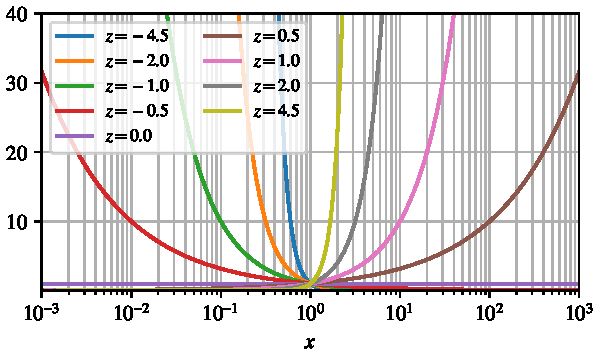
\includegraphics{papers/laguerre/images/integrand.pdf}
%\vspace{-12pt}
\caption{Integrand $x^z$ mit unterschiedlichen Werten für $z$}
\label{laguerre:fig:integrand}
\end{figure}

In Abbildung~\ref{laguerre:fig:integrand} ist der Integrand $x^z$ für
unterschiedliche Werte von $z$ dargestellt.
Dies entspricht der zu integrierenden Funktion $f(x)$
der Gauss-Laguerre-Quadratur für die Gamma-Funktion.
Man erkennt,
dass für kleine $z$ sich ein singulärer Integrand ergibt
und auch für grosse $z$ wächst der Integrand sehr schnell an.
Das heisst,
die Ableitungen im Fehlerterm divergieren noch schneller
und das wirkt sich negativ auf die Genauigkeit der Approximation aus.
Somit lässt sich hier sagen,
dass kleine Exponenten um $0$ genauere Resultate liefern sollten.

\begin{figure}
\centering
% %% Creator: Matplotlib, PGF backend
%%
%% To include the figure in your LaTeX document, write
%%   \input{<filename>.pgf}
%%
%% Make sure the required packages are loaded in your preamble
%%   \usepackage{pgf}
%%
%% Also ensure that all the required font packages are loaded; for instance,
%% the lmodern package is sometimes necessary when using math font.
%%   \usepackage{lmodern}
%%
%% Figures using additional raster images can only be included by \input if
%% they are in the same directory as the main LaTeX file. For loading figures
%% from other directories you can use the `import` package
%%   \usepackage{import}
%%
%% and then include the figures with
%%   \import{<path to file>}{<filename>.pgf}
%%
%% Matplotlib used the following preamble
%%   \usepackage{fontspec}
%%   \setmainfont{DejaVuSerif.ttf}[Path=\detokenize{/home/mup/.local/lib/python3.8/site-packages/matplotlib/mpl-data/fonts/ttf/}]
%%   \setsansfont{DejaVuSans.ttf}[Path=\detokenize{/home/mup/.local/lib/python3.8/site-packages/matplotlib/mpl-data/fonts/ttf/}]
%%   \setmonofont{DejaVuSansMono.ttf}[Path=\detokenize{/home/mup/.local/lib/python3.8/site-packages/matplotlib/mpl-data/fonts/ttf/}]
%%
\begingroup%
\makeatletter%
\begin{pgfpicture}%
\pgfpathrectangle{\pgfpointorigin}{\pgfqpoint{4.000000in}{2.400000in}}%
\pgfusepath{use as bounding box, clip}%
\begin{pgfscope}%
\pgfsetbuttcap%
\pgfsetmiterjoin%
\definecolor{currentfill}{rgb}{1.000000,1.000000,1.000000}%
\pgfsetfillcolor{currentfill}%
\pgfsetlinewidth{0.000000pt}%
\definecolor{currentstroke}{rgb}{1.000000,1.000000,1.000000}%
\pgfsetstrokecolor{currentstroke}%
\pgfsetdash{}{0pt}%
\pgfpathmoveto{\pgfqpoint{0.000000in}{0.000000in}}%
\pgfpathlineto{\pgfqpoint{4.000000in}{0.000000in}}%
\pgfpathlineto{\pgfqpoint{4.000000in}{2.400000in}}%
\pgfpathlineto{\pgfqpoint{0.000000in}{2.400000in}}%
\pgfpathlineto{\pgfqpoint{0.000000in}{0.000000in}}%
\pgfpathclose%
\pgfusepath{fill}%
\end{pgfscope}%
\begin{pgfscope}%
\pgfsetbuttcap%
\pgfsetmiterjoin%
\definecolor{currentfill}{rgb}{1.000000,1.000000,1.000000}%
\pgfsetfillcolor{currentfill}%
\pgfsetlinewidth{0.000000pt}%
\definecolor{currentstroke}{rgb}{0.000000,0.000000,0.000000}%
\pgfsetstrokecolor{currentstroke}%
\pgfsetstrokeopacity{0.000000}%
\pgfsetdash{}{0pt}%
\pgfpathmoveto{\pgfqpoint{0.315623in}{0.463273in}}%
\pgfpathlineto{\pgfqpoint{3.958330in}{0.463273in}}%
\pgfpathlineto{\pgfqpoint{3.958330in}{2.305568in}}%
\pgfpathlineto{\pgfqpoint{0.315623in}{2.305568in}}%
\pgfpathlineto{\pgfqpoint{0.315623in}{0.463273in}}%
\pgfpathclose%
\pgfusepath{fill}%
\end{pgfscope}%
\begin{pgfscope}%
\pgfpathrectangle{\pgfqpoint{0.315623in}{0.463273in}}{\pgfqpoint{3.642707in}{1.842295in}}%
\pgfusepath{clip}%
\pgfsetrectcap%
\pgfsetroundjoin%
\pgfsetlinewidth{0.803000pt}%
\definecolor{currentstroke}{rgb}{0.690196,0.690196,0.690196}%
\pgfsetstrokecolor{currentstroke}%
\pgfsetdash{}{0pt}%
\pgfpathmoveto{\pgfqpoint{0.315623in}{0.463273in}}%
\pgfpathlineto{\pgfqpoint{0.315623in}{2.305568in}}%
\pgfusepath{stroke}%
\end{pgfscope}%
\begin{pgfscope}%
\pgfsetbuttcap%
\pgfsetroundjoin%
\definecolor{currentfill}{rgb}{0.000000,0.000000,0.000000}%
\pgfsetfillcolor{currentfill}%
\pgfsetlinewidth{0.803000pt}%
\definecolor{currentstroke}{rgb}{0.000000,0.000000,0.000000}%
\pgfsetstrokecolor{currentstroke}%
\pgfsetdash{}{0pt}%
\pgfsys@defobject{currentmarker}{\pgfqpoint{0.000000in}{-0.048611in}}{\pgfqpoint{0.000000in}{0.000000in}}{%
\pgfpathmoveto{\pgfqpoint{0.000000in}{0.000000in}}%
\pgfpathlineto{\pgfqpoint{0.000000in}{-0.048611in}}%
\pgfusepath{stroke,fill}%
}%
\begin{pgfscope}%
\pgfsys@transformshift{0.315623in}{0.463273in}%
\pgfsys@useobject{currentmarker}{}%
\end{pgfscope}%
\end{pgfscope}%
\begin{pgfscope}%
\definecolor{textcolor}{rgb}{0.000000,0.000000,0.000000}%
\pgfsetstrokecolor{textcolor}%
\pgfsetfillcolor{textcolor}%
\pgftext[x=0.315623in,y=0.366051in,,top]{\color{textcolor}\sffamily\fontsize{10.000000}{12.000000}\selectfont \(\displaystyle {10^{-2}}\)}%
\end{pgfscope}%
\begin{pgfscope}%
\pgfpathrectangle{\pgfqpoint{0.315623in}{0.463273in}}{\pgfqpoint{3.642707in}{1.842295in}}%
\pgfusepath{clip}%
\pgfsetrectcap%
\pgfsetroundjoin%
\pgfsetlinewidth{0.803000pt}%
\definecolor{currentstroke}{rgb}{0.690196,0.690196,0.690196}%
\pgfsetstrokecolor{currentstroke}%
\pgfsetdash{}{0pt}%
\pgfpathmoveto{\pgfqpoint{1.419129in}{0.463273in}}%
\pgfpathlineto{\pgfqpoint{1.419129in}{2.305568in}}%
\pgfusepath{stroke}%
\end{pgfscope}%
\begin{pgfscope}%
\pgfsetbuttcap%
\pgfsetroundjoin%
\definecolor{currentfill}{rgb}{0.000000,0.000000,0.000000}%
\pgfsetfillcolor{currentfill}%
\pgfsetlinewidth{0.803000pt}%
\definecolor{currentstroke}{rgb}{0.000000,0.000000,0.000000}%
\pgfsetstrokecolor{currentstroke}%
\pgfsetdash{}{0pt}%
\pgfsys@defobject{currentmarker}{\pgfqpoint{0.000000in}{-0.048611in}}{\pgfqpoint{0.000000in}{0.000000in}}{%
\pgfpathmoveto{\pgfqpoint{0.000000in}{0.000000in}}%
\pgfpathlineto{\pgfqpoint{0.000000in}{-0.048611in}}%
\pgfusepath{stroke,fill}%
}%
\begin{pgfscope}%
\pgfsys@transformshift{1.419129in}{0.463273in}%
\pgfsys@useobject{currentmarker}{}%
\end{pgfscope}%
\end{pgfscope}%
\begin{pgfscope}%
\definecolor{textcolor}{rgb}{0.000000,0.000000,0.000000}%
\pgfsetstrokecolor{textcolor}%
\pgfsetfillcolor{textcolor}%
\pgftext[x=1.419129in,y=0.366051in,,top]{\color{textcolor}\sffamily\fontsize{10.000000}{12.000000}\selectfont \(\displaystyle {10^{-1}}\)}%
\end{pgfscope}%
\begin{pgfscope}%
\pgfpathrectangle{\pgfqpoint{0.315623in}{0.463273in}}{\pgfqpoint{3.642707in}{1.842295in}}%
\pgfusepath{clip}%
\pgfsetrectcap%
\pgfsetroundjoin%
\pgfsetlinewidth{0.803000pt}%
\definecolor{currentstroke}{rgb}{0.690196,0.690196,0.690196}%
\pgfsetstrokecolor{currentstroke}%
\pgfsetdash{}{0pt}%
\pgfpathmoveto{\pgfqpoint{2.522635in}{0.463273in}}%
\pgfpathlineto{\pgfqpoint{2.522635in}{2.305568in}}%
\pgfusepath{stroke}%
\end{pgfscope}%
\begin{pgfscope}%
\pgfsetbuttcap%
\pgfsetroundjoin%
\definecolor{currentfill}{rgb}{0.000000,0.000000,0.000000}%
\pgfsetfillcolor{currentfill}%
\pgfsetlinewidth{0.803000pt}%
\definecolor{currentstroke}{rgb}{0.000000,0.000000,0.000000}%
\pgfsetstrokecolor{currentstroke}%
\pgfsetdash{}{0pt}%
\pgfsys@defobject{currentmarker}{\pgfqpoint{0.000000in}{-0.048611in}}{\pgfqpoint{0.000000in}{0.000000in}}{%
\pgfpathmoveto{\pgfqpoint{0.000000in}{0.000000in}}%
\pgfpathlineto{\pgfqpoint{0.000000in}{-0.048611in}}%
\pgfusepath{stroke,fill}%
}%
\begin{pgfscope}%
\pgfsys@transformshift{2.522635in}{0.463273in}%
\pgfsys@useobject{currentmarker}{}%
\end{pgfscope}%
\end{pgfscope}%
\begin{pgfscope}%
\definecolor{textcolor}{rgb}{0.000000,0.000000,0.000000}%
\pgfsetstrokecolor{textcolor}%
\pgfsetfillcolor{textcolor}%
\pgftext[x=2.522635in,y=0.366051in,,top]{\color{textcolor}\sffamily\fontsize{10.000000}{12.000000}\selectfont \(\displaystyle {10^{0}}\)}%
\end{pgfscope}%
\begin{pgfscope}%
\pgfpathrectangle{\pgfqpoint{0.315623in}{0.463273in}}{\pgfqpoint{3.642707in}{1.842295in}}%
\pgfusepath{clip}%
\pgfsetrectcap%
\pgfsetroundjoin%
\pgfsetlinewidth{0.803000pt}%
\definecolor{currentstroke}{rgb}{0.690196,0.690196,0.690196}%
\pgfsetstrokecolor{currentstroke}%
\pgfsetdash{}{0pt}%
\pgfpathmoveto{\pgfqpoint{3.626142in}{0.463273in}}%
\pgfpathlineto{\pgfqpoint{3.626142in}{2.305568in}}%
\pgfusepath{stroke}%
\end{pgfscope}%
\begin{pgfscope}%
\pgfsetbuttcap%
\pgfsetroundjoin%
\definecolor{currentfill}{rgb}{0.000000,0.000000,0.000000}%
\pgfsetfillcolor{currentfill}%
\pgfsetlinewidth{0.803000pt}%
\definecolor{currentstroke}{rgb}{0.000000,0.000000,0.000000}%
\pgfsetstrokecolor{currentstroke}%
\pgfsetdash{}{0pt}%
\pgfsys@defobject{currentmarker}{\pgfqpoint{0.000000in}{-0.048611in}}{\pgfqpoint{0.000000in}{0.000000in}}{%
\pgfpathmoveto{\pgfqpoint{0.000000in}{0.000000in}}%
\pgfpathlineto{\pgfqpoint{0.000000in}{-0.048611in}}%
\pgfusepath{stroke,fill}%
}%
\begin{pgfscope}%
\pgfsys@transformshift{3.626142in}{0.463273in}%
\pgfsys@useobject{currentmarker}{}%
\end{pgfscope}%
\end{pgfscope}%
\begin{pgfscope}%
\definecolor{textcolor}{rgb}{0.000000,0.000000,0.000000}%
\pgfsetstrokecolor{textcolor}%
\pgfsetfillcolor{textcolor}%
\pgftext[x=3.626142in,y=0.366051in,,top]{\color{textcolor}\sffamily\fontsize{10.000000}{12.000000}\selectfont \(\displaystyle {10^{1}}\)}%
\end{pgfscope}%
\begin{pgfscope}%
\pgfpathrectangle{\pgfqpoint{0.315623in}{0.463273in}}{\pgfqpoint{3.642707in}{1.842295in}}%
\pgfusepath{clip}%
\pgfsetrectcap%
\pgfsetroundjoin%
\pgfsetlinewidth{0.803000pt}%
\definecolor{currentstroke}{rgb}{0.690196,0.690196,0.690196}%
\pgfsetstrokecolor{currentstroke}%
\pgfsetdash{}{0pt}%
\pgfpathmoveto{\pgfqpoint{0.647811in}{0.463273in}}%
\pgfpathlineto{\pgfqpoint{0.647811in}{2.305568in}}%
\pgfusepath{stroke}%
\end{pgfscope}%
\begin{pgfscope}%
\pgfsetbuttcap%
\pgfsetroundjoin%
\definecolor{currentfill}{rgb}{0.000000,0.000000,0.000000}%
\pgfsetfillcolor{currentfill}%
\pgfsetlinewidth{0.602250pt}%
\definecolor{currentstroke}{rgb}{0.000000,0.000000,0.000000}%
\pgfsetstrokecolor{currentstroke}%
\pgfsetdash{}{0pt}%
\pgfsys@defobject{currentmarker}{\pgfqpoint{0.000000in}{-0.027778in}}{\pgfqpoint{0.000000in}{0.000000in}}{%
\pgfpathmoveto{\pgfqpoint{0.000000in}{0.000000in}}%
\pgfpathlineto{\pgfqpoint{0.000000in}{-0.027778in}}%
\pgfusepath{stroke,fill}%
}%
\begin{pgfscope}%
\pgfsys@transformshift{0.647811in}{0.463273in}%
\pgfsys@useobject{currentmarker}{}%
\end{pgfscope}%
\end{pgfscope}%
\begin{pgfscope}%
\pgfpathrectangle{\pgfqpoint{0.315623in}{0.463273in}}{\pgfqpoint{3.642707in}{1.842295in}}%
\pgfusepath{clip}%
\pgfsetrectcap%
\pgfsetroundjoin%
\pgfsetlinewidth{0.803000pt}%
\definecolor{currentstroke}{rgb}{0.690196,0.690196,0.690196}%
\pgfsetstrokecolor{currentstroke}%
\pgfsetdash{}{0pt}%
\pgfpathmoveto{\pgfqpoint{0.842129in}{0.463273in}}%
\pgfpathlineto{\pgfqpoint{0.842129in}{2.305568in}}%
\pgfusepath{stroke}%
\end{pgfscope}%
\begin{pgfscope}%
\pgfsetbuttcap%
\pgfsetroundjoin%
\definecolor{currentfill}{rgb}{0.000000,0.000000,0.000000}%
\pgfsetfillcolor{currentfill}%
\pgfsetlinewidth{0.602250pt}%
\definecolor{currentstroke}{rgb}{0.000000,0.000000,0.000000}%
\pgfsetstrokecolor{currentstroke}%
\pgfsetdash{}{0pt}%
\pgfsys@defobject{currentmarker}{\pgfqpoint{0.000000in}{-0.027778in}}{\pgfqpoint{0.000000in}{0.000000in}}{%
\pgfpathmoveto{\pgfqpoint{0.000000in}{0.000000in}}%
\pgfpathlineto{\pgfqpoint{0.000000in}{-0.027778in}}%
\pgfusepath{stroke,fill}%
}%
\begin{pgfscope}%
\pgfsys@transformshift{0.842129in}{0.463273in}%
\pgfsys@useobject{currentmarker}{}%
\end{pgfscope}%
\end{pgfscope}%
\begin{pgfscope}%
\pgfpathrectangle{\pgfqpoint{0.315623in}{0.463273in}}{\pgfqpoint{3.642707in}{1.842295in}}%
\pgfusepath{clip}%
\pgfsetrectcap%
\pgfsetroundjoin%
\pgfsetlinewidth{0.803000pt}%
\definecolor{currentstroke}{rgb}{0.690196,0.690196,0.690196}%
\pgfsetstrokecolor{currentstroke}%
\pgfsetdash{}{0pt}%
\pgfpathmoveto{\pgfqpoint{0.980000in}{0.463273in}}%
\pgfpathlineto{\pgfqpoint{0.980000in}{2.305568in}}%
\pgfusepath{stroke}%
\end{pgfscope}%
\begin{pgfscope}%
\pgfsetbuttcap%
\pgfsetroundjoin%
\definecolor{currentfill}{rgb}{0.000000,0.000000,0.000000}%
\pgfsetfillcolor{currentfill}%
\pgfsetlinewidth{0.602250pt}%
\definecolor{currentstroke}{rgb}{0.000000,0.000000,0.000000}%
\pgfsetstrokecolor{currentstroke}%
\pgfsetdash{}{0pt}%
\pgfsys@defobject{currentmarker}{\pgfqpoint{0.000000in}{-0.027778in}}{\pgfqpoint{0.000000in}{0.000000in}}{%
\pgfpathmoveto{\pgfqpoint{0.000000in}{0.000000in}}%
\pgfpathlineto{\pgfqpoint{0.000000in}{-0.027778in}}%
\pgfusepath{stroke,fill}%
}%
\begin{pgfscope}%
\pgfsys@transformshift{0.980000in}{0.463273in}%
\pgfsys@useobject{currentmarker}{}%
\end{pgfscope}%
\end{pgfscope}%
\begin{pgfscope}%
\pgfpathrectangle{\pgfqpoint{0.315623in}{0.463273in}}{\pgfqpoint{3.642707in}{1.842295in}}%
\pgfusepath{clip}%
\pgfsetrectcap%
\pgfsetroundjoin%
\pgfsetlinewidth{0.803000pt}%
\definecolor{currentstroke}{rgb}{0.690196,0.690196,0.690196}%
\pgfsetstrokecolor{currentstroke}%
\pgfsetdash{}{0pt}%
\pgfpathmoveto{\pgfqpoint{1.086941in}{0.463273in}}%
\pgfpathlineto{\pgfqpoint{1.086941in}{2.305568in}}%
\pgfusepath{stroke}%
\end{pgfscope}%
\begin{pgfscope}%
\pgfsetbuttcap%
\pgfsetroundjoin%
\definecolor{currentfill}{rgb}{0.000000,0.000000,0.000000}%
\pgfsetfillcolor{currentfill}%
\pgfsetlinewidth{0.602250pt}%
\definecolor{currentstroke}{rgb}{0.000000,0.000000,0.000000}%
\pgfsetstrokecolor{currentstroke}%
\pgfsetdash{}{0pt}%
\pgfsys@defobject{currentmarker}{\pgfqpoint{0.000000in}{-0.027778in}}{\pgfqpoint{0.000000in}{0.000000in}}{%
\pgfpathmoveto{\pgfqpoint{0.000000in}{0.000000in}}%
\pgfpathlineto{\pgfqpoint{0.000000in}{-0.027778in}}%
\pgfusepath{stroke,fill}%
}%
\begin{pgfscope}%
\pgfsys@transformshift{1.086941in}{0.463273in}%
\pgfsys@useobject{currentmarker}{}%
\end{pgfscope}%
\end{pgfscope}%
\begin{pgfscope}%
\pgfpathrectangle{\pgfqpoint{0.315623in}{0.463273in}}{\pgfqpoint{3.642707in}{1.842295in}}%
\pgfusepath{clip}%
\pgfsetrectcap%
\pgfsetroundjoin%
\pgfsetlinewidth{0.803000pt}%
\definecolor{currentstroke}{rgb}{0.690196,0.690196,0.690196}%
\pgfsetstrokecolor{currentstroke}%
\pgfsetdash{}{0pt}%
\pgfpathmoveto{\pgfqpoint{1.174318in}{0.463273in}}%
\pgfpathlineto{\pgfqpoint{1.174318in}{2.305568in}}%
\pgfusepath{stroke}%
\end{pgfscope}%
\begin{pgfscope}%
\pgfsetbuttcap%
\pgfsetroundjoin%
\definecolor{currentfill}{rgb}{0.000000,0.000000,0.000000}%
\pgfsetfillcolor{currentfill}%
\pgfsetlinewidth{0.602250pt}%
\definecolor{currentstroke}{rgb}{0.000000,0.000000,0.000000}%
\pgfsetstrokecolor{currentstroke}%
\pgfsetdash{}{0pt}%
\pgfsys@defobject{currentmarker}{\pgfqpoint{0.000000in}{-0.027778in}}{\pgfqpoint{0.000000in}{0.000000in}}{%
\pgfpathmoveto{\pgfqpoint{0.000000in}{0.000000in}}%
\pgfpathlineto{\pgfqpoint{0.000000in}{-0.027778in}}%
\pgfusepath{stroke,fill}%
}%
\begin{pgfscope}%
\pgfsys@transformshift{1.174318in}{0.463273in}%
\pgfsys@useobject{currentmarker}{}%
\end{pgfscope}%
\end{pgfscope}%
\begin{pgfscope}%
\pgfpathrectangle{\pgfqpoint{0.315623in}{0.463273in}}{\pgfqpoint{3.642707in}{1.842295in}}%
\pgfusepath{clip}%
\pgfsetrectcap%
\pgfsetroundjoin%
\pgfsetlinewidth{0.803000pt}%
\definecolor{currentstroke}{rgb}{0.690196,0.690196,0.690196}%
\pgfsetstrokecolor{currentstroke}%
\pgfsetdash{}{0pt}%
\pgfpathmoveto{\pgfqpoint{1.248194in}{0.463273in}}%
\pgfpathlineto{\pgfqpoint{1.248194in}{2.305568in}}%
\pgfusepath{stroke}%
\end{pgfscope}%
\begin{pgfscope}%
\pgfsetbuttcap%
\pgfsetroundjoin%
\definecolor{currentfill}{rgb}{0.000000,0.000000,0.000000}%
\pgfsetfillcolor{currentfill}%
\pgfsetlinewidth{0.602250pt}%
\definecolor{currentstroke}{rgb}{0.000000,0.000000,0.000000}%
\pgfsetstrokecolor{currentstroke}%
\pgfsetdash{}{0pt}%
\pgfsys@defobject{currentmarker}{\pgfqpoint{0.000000in}{-0.027778in}}{\pgfqpoint{0.000000in}{0.000000in}}{%
\pgfpathmoveto{\pgfqpoint{0.000000in}{0.000000in}}%
\pgfpathlineto{\pgfqpoint{0.000000in}{-0.027778in}}%
\pgfusepath{stroke,fill}%
}%
\begin{pgfscope}%
\pgfsys@transformshift{1.248194in}{0.463273in}%
\pgfsys@useobject{currentmarker}{}%
\end{pgfscope}%
\end{pgfscope}%
\begin{pgfscope}%
\pgfpathrectangle{\pgfqpoint{0.315623in}{0.463273in}}{\pgfqpoint{3.642707in}{1.842295in}}%
\pgfusepath{clip}%
\pgfsetrectcap%
\pgfsetroundjoin%
\pgfsetlinewidth{0.803000pt}%
\definecolor{currentstroke}{rgb}{0.690196,0.690196,0.690196}%
\pgfsetstrokecolor{currentstroke}%
\pgfsetdash{}{0pt}%
\pgfpathmoveto{\pgfqpoint{1.312188in}{0.463273in}}%
\pgfpathlineto{\pgfqpoint{1.312188in}{2.305568in}}%
\pgfusepath{stroke}%
\end{pgfscope}%
\begin{pgfscope}%
\pgfsetbuttcap%
\pgfsetroundjoin%
\definecolor{currentfill}{rgb}{0.000000,0.000000,0.000000}%
\pgfsetfillcolor{currentfill}%
\pgfsetlinewidth{0.602250pt}%
\definecolor{currentstroke}{rgb}{0.000000,0.000000,0.000000}%
\pgfsetstrokecolor{currentstroke}%
\pgfsetdash{}{0pt}%
\pgfsys@defobject{currentmarker}{\pgfqpoint{0.000000in}{-0.027778in}}{\pgfqpoint{0.000000in}{0.000000in}}{%
\pgfpathmoveto{\pgfqpoint{0.000000in}{0.000000in}}%
\pgfpathlineto{\pgfqpoint{0.000000in}{-0.027778in}}%
\pgfusepath{stroke,fill}%
}%
\begin{pgfscope}%
\pgfsys@transformshift{1.312188in}{0.463273in}%
\pgfsys@useobject{currentmarker}{}%
\end{pgfscope}%
\end{pgfscope}%
\begin{pgfscope}%
\pgfpathrectangle{\pgfqpoint{0.315623in}{0.463273in}}{\pgfqpoint{3.642707in}{1.842295in}}%
\pgfusepath{clip}%
\pgfsetrectcap%
\pgfsetroundjoin%
\pgfsetlinewidth{0.803000pt}%
\definecolor{currentstroke}{rgb}{0.690196,0.690196,0.690196}%
\pgfsetstrokecolor{currentstroke}%
\pgfsetdash{}{0pt}%
\pgfpathmoveto{\pgfqpoint{1.368635in}{0.463273in}}%
\pgfpathlineto{\pgfqpoint{1.368635in}{2.305568in}}%
\pgfusepath{stroke}%
\end{pgfscope}%
\begin{pgfscope}%
\pgfsetbuttcap%
\pgfsetroundjoin%
\definecolor{currentfill}{rgb}{0.000000,0.000000,0.000000}%
\pgfsetfillcolor{currentfill}%
\pgfsetlinewidth{0.602250pt}%
\definecolor{currentstroke}{rgb}{0.000000,0.000000,0.000000}%
\pgfsetstrokecolor{currentstroke}%
\pgfsetdash{}{0pt}%
\pgfsys@defobject{currentmarker}{\pgfqpoint{0.000000in}{-0.027778in}}{\pgfqpoint{0.000000in}{0.000000in}}{%
\pgfpathmoveto{\pgfqpoint{0.000000in}{0.000000in}}%
\pgfpathlineto{\pgfqpoint{0.000000in}{-0.027778in}}%
\pgfusepath{stroke,fill}%
}%
\begin{pgfscope}%
\pgfsys@transformshift{1.368635in}{0.463273in}%
\pgfsys@useobject{currentmarker}{}%
\end{pgfscope}%
\end{pgfscope}%
\begin{pgfscope}%
\pgfpathrectangle{\pgfqpoint{0.315623in}{0.463273in}}{\pgfqpoint{3.642707in}{1.842295in}}%
\pgfusepath{clip}%
\pgfsetrectcap%
\pgfsetroundjoin%
\pgfsetlinewidth{0.803000pt}%
\definecolor{currentstroke}{rgb}{0.690196,0.690196,0.690196}%
\pgfsetstrokecolor{currentstroke}%
\pgfsetdash{}{0pt}%
\pgfpathmoveto{\pgfqpoint{1.751318in}{0.463273in}}%
\pgfpathlineto{\pgfqpoint{1.751318in}{2.305568in}}%
\pgfusepath{stroke}%
\end{pgfscope}%
\begin{pgfscope}%
\pgfsetbuttcap%
\pgfsetroundjoin%
\definecolor{currentfill}{rgb}{0.000000,0.000000,0.000000}%
\pgfsetfillcolor{currentfill}%
\pgfsetlinewidth{0.602250pt}%
\definecolor{currentstroke}{rgb}{0.000000,0.000000,0.000000}%
\pgfsetstrokecolor{currentstroke}%
\pgfsetdash{}{0pt}%
\pgfsys@defobject{currentmarker}{\pgfqpoint{0.000000in}{-0.027778in}}{\pgfqpoint{0.000000in}{0.000000in}}{%
\pgfpathmoveto{\pgfqpoint{0.000000in}{0.000000in}}%
\pgfpathlineto{\pgfqpoint{0.000000in}{-0.027778in}}%
\pgfusepath{stroke,fill}%
}%
\begin{pgfscope}%
\pgfsys@transformshift{1.751318in}{0.463273in}%
\pgfsys@useobject{currentmarker}{}%
\end{pgfscope}%
\end{pgfscope}%
\begin{pgfscope}%
\pgfpathrectangle{\pgfqpoint{0.315623in}{0.463273in}}{\pgfqpoint{3.642707in}{1.842295in}}%
\pgfusepath{clip}%
\pgfsetrectcap%
\pgfsetroundjoin%
\pgfsetlinewidth{0.803000pt}%
\definecolor{currentstroke}{rgb}{0.690196,0.690196,0.690196}%
\pgfsetstrokecolor{currentstroke}%
\pgfsetdash{}{0pt}%
\pgfpathmoveto{\pgfqpoint{1.945635in}{0.463273in}}%
\pgfpathlineto{\pgfqpoint{1.945635in}{2.305568in}}%
\pgfusepath{stroke}%
\end{pgfscope}%
\begin{pgfscope}%
\pgfsetbuttcap%
\pgfsetroundjoin%
\definecolor{currentfill}{rgb}{0.000000,0.000000,0.000000}%
\pgfsetfillcolor{currentfill}%
\pgfsetlinewidth{0.602250pt}%
\definecolor{currentstroke}{rgb}{0.000000,0.000000,0.000000}%
\pgfsetstrokecolor{currentstroke}%
\pgfsetdash{}{0pt}%
\pgfsys@defobject{currentmarker}{\pgfqpoint{0.000000in}{-0.027778in}}{\pgfqpoint{0.000000in}{0.000000in}}{%
\pgfpathmoveto{\pgfqpoint{0.000000in}{0.000000in}}%
\pgfpathlineto{\pgfqpoint{0.000000in}{-0.027778in}}%
\pgfusepath{stroke,fill}%
}%
\begin{pgfscope}%
\pgfsys@transformshift{1.945635in}{0.463273in}%
\pgfsys@useobject{currentmarker}{}%
\end{pgfscope}%
\end{pgfscope}%
\begin{pgfscope}%
\pgfpathrectangle{\pgfqpoint{0.315623in}{0.463273in}}{\pgfqpoint{3.642707in}{1.842295in}}%
\pgfusepath{clip}%
\pgfsetrectcap%
\pgfsetroundjoin%
\pgfsetlinewidth{0.803000pt}%
\definecolor{currentstroke}{rgb}{0.690196,0.690196,0.690196}%
\pgfsetstrokecolor{currentstroke}%
\pgfsetdash{}{0pt}%
\pgfpathmoveto{\pgfqpoint{2.083506in}{0.463273in}}%
\pgfpathlineto{\pgfqpoint{2.083506in}{2.305568in}}%
\pgfusepath{stroke}%
\end{pgfscope}%
\begin{pgfscope}%
\pgfsetbuttcap%
\pgfsetroundjoin%
\definecolor{currentfill}{rgb}{0.000000,0.000000,0.000000}%
\pgfsetfillcolor{currentfill}%
\pgfsetlinewidth{0.602250pt}%
\definecolor{currentstroke}{rgb}{0.000000,0.000000,0.000000}%
\pgfsetstrokecolor{currentstroke}%
\pgfsetdash{}{0pt}%
\pgfsys@defobject{currentmarker}{\pgfqpoint{0.000000in}{-0.027778in}}{\pgfqpoint{0.000000in}{0.000000in}}{%
\pgfpathmoveto{\pgfqpoint{0.000000in}{0.000000in}}%
\pgfpathlineto{\pgfqpoint{0.000000in}{-0.027778in}}%
\pgfusepath{stroke,fill}%
}%
\begin{pgfscope}%
\pgfsys@transformshift{2.083506in}{0.463273in}%
\pgfsys@useobject{currentmarker}{}%
\end{pgfscope}%
\end{pgfscope}%
\begin{pgfscope}%
\pgfpathrectangle{\pgfqpoint{0.315623in}{0.463273in}}{\pgfqpoint{3.642707in}{1.842295in}}%
\pgfusepath{clip}%
\pgfsetrectcap%
\pgfsetroundjoin%
\pgfsetlinewidth{0.803000pt}%
\definecolor{currentstroke}{rgb}{0.690196,0.690196,0.690196}%
\pgfsetstrokecolor{currentstroke}%
\pgfsetdash{}{0pt}%
\pgfpathmoveto{\pgfqpoint{2.190447in}{0.463273in}}%
\pgfpathlineto{\pgfqpoint{2.190447in}{2.305568in}}%
\pgfusepath{stroke}%
\end{pgfscope}%
\begin{pgfscope}%
\pgfsetbuttcap%
\pgfsetroundjoin%
\definecolor{currentfill}{rgb}{0.000000,0.000000,0.000000}%
\pgfsetfillcolor{currentfill}%
\pgfsetlinewidth{0.602250pt}%
\definecolor{currentstroke}{rgb}{0.000000,0.000000,0.000000}%
\pgfsetstrokecolor{currentstroke}%
\pgfsetdash{}{0pt}%
\pgfsys@defobject{currentmarker}{\pgfqpoint{0.000000in}{-0.027778in}}{\pgfqpoint{0.000000in}{0.000000in}}{%
\pgfpathmoveto{\pgfqpoint{0.000000in}{0.000000in}}%
\pgfpathlineto{\pgfqpoint{0.000000in}{-0.027778in}}%
\pgfusepath{stroke,fill}%
}%
\begin{pgfscope}%
\pgfsys@transformshift{2.190447in}{0.463273in}%
\pgfsys@useobject{currentmarker}{}%
\end{pgfscope}%
\end{pgfscope}%
\begin{pgfscope}%
\pgfpathrectangle{\pgfqpoint{0.315623in}{0.463273in}}{\pgfqpoint{3.642707in}{1.842295in}}%
\pgfusepath{clip}%
\pgfsetrectcap%
\pgfsetroundjoin%
\pgfsetlinewidth{0.803000pt}%
\definecolor{currentstroke}{rgb}{0.690196,0.690196,0.690196}%
\pgfsetstrokecolor{currentstroke}%
\pgfsetdash{}{0pt}%
\pgfpathmoveto{\pgfqpoint{2.277824in}{0.463273in}}%
\pgfpathlineto{\pgfqpoint{2.277824in}{2.305568in}}%
\pgfusepath{stroke}%
\end{pgfscope}%
\begin{pgfscope}%
\pgfsetbuttcap%
\pgfsetroundjoin%
\definecolor{currentfill}{rgb}{0.000000,0.000000,0.000000}%
\pgfsetfillcolor{currentfill}%
\pgfsetlinewidth{0.602250pt}%
\definecolor{currentstroke}{rgb}{0.000000,0.000000,0.000000}%
\pgfsetstrokecolor{currentstroke}%
\pgfsetdash{}{0pt}%
\pgfsys@defobject{currentmarker}{\pgfqpoint{0.000000in}{-0.027778in}}{\pgfqpoint{0.000000in}{0.000000in}}{%
\pgfpathmoveto{\pgfqpoint{0.000000in}{0.000000in}}%
\pgfpathlineto{\pgfqpoint{0.000000in}{-0.027778in}}%
\pgfusepath{stroke,fill}%
}%
\begin{pgfscope}%
\pgfsys@transformshift{2.277824in}{0.463273in}%
\pgfsys@useobject{currentmarker}{}%
\end{pgfscope}%
\end{pgfscope}%
\begin{pgfscope}%
\pgfpathrectangle{\pgfqpoint{0.315623in}{0.463273in}}{\pgfqpoint{3.642707in}{1.842295in}}%
\pgfusepath{clip}%
\pgfsetrectcap%
\pgfsetroundjoin%
\pgfsetlinewidth{0.803000pt}%
\definecolor{currentstroke}{rgb}{0.690196,0.690196,0.690196}%
\pgfsetstrokecolor{currentstroke}%
\pgfsetdash{}{0pt}%
\pgfpathmoveto{\pgfqpoint{2.351700in}{0.463273in}}%
\pgfpathlineto{\pgfqpoint{2.351700in}{2.305568in}}%
\pgfusepath{stroke}%
\end{pgfscope}%
\begin{pgfscope}%
\pgfsetbuttcap%
\pgfsetroundjoin%
\definecolor{currentfill}{rgb}{0.000000,0.000000,0.000000}%
\pgfsetfillcolor{currentfill}%
\pgfsetlinewidth{0.602250pt}%
\definecolor{currentstroke}{rgb}{0.000000,0.000000,0.000000}%
\pgfsetstrokecolor{currentstroke}%
\pgfsetdash{}{0pt}%
\pgfsys@defobject{currentmarker}{\pgfqpoint{0.000000in}{-0.027778in}}{\pgfqpoint{0.000000in}{0.000000in}}{%
\pgfpathmoveto{\pgfqpoint{0.000000in}{0.000000in}}%
\pgfpathlineto{\pgfqpoint{0.000000in}{-0.027778in}}%
\pgfusepath{stroke,fill}%
}%
\begin{pgfscope}%
\pgfsys@transformshift{2.351700in}{0.463273in}%
\pgfsys@useobject{currentmarker}{}%
\end{pgfscope}%
\end{pgfscope}%
\begin{pgfscope}%
\pgfpathrectangle{\pgfqpoint{0.315623in}{0.463273in}}{\pgfqpoint{3.642707in}{1.842295in}}%
\pgfusepath{clip}%
\pgfsetrectcap%
\pgfsetroundjoin%
\pgfsetlinewidth{0.803000pt}%
\definecolor{currentstroke}{rgb}{0.690196,0.690196,0.690196}%
\pgfsetstrokecolor{currentstroke}%
\pgfsetdash{}{0pt}%
\pgfpathmoveto{\pgfqpoint{2.415695in}{0.463273in}}%
\pgfpathlineto{\pgfqpoint{2.415695in}{2.305568in}}%
\pgfusepath{stroke}%
\end{pgfscope}%
\begin{pgfscope}%
\pgfsetbuttcap%
\pgfsetroundjoin%
\definecolor{currentfill}{rgb}{0.000000,0.000000,0.000000}%
\pgfsetfillcolor{currentfill}%
\pgfsetlinewidth{0.602250pt}%
\definecolor{currentstroke}{rgb}{0.000000,0.000000,0.000000}%
\pgfsetstrokecolor{currentstroke}%
\pgfsetdash{}{0pt}%
\pgfsys@defobject{currentmarker}{\pgfqpoint{0.000000in}{-0.027778in}}{\pgfqpoint{0.000000in}{0.000000in}}{%
\pgfpathmoveto{\pgfqpoint{0.000000in}{0.000000in}}%
\pgfpathlineto{\pgfqpoint{0.000000in}{-0.027778in}}%
\pgfusepath{stroke,fill}%
}%
\begin{pgfscope}%
\pgfsys@transformshift{2.415695in}{0.463273in}%
\pgfsys@useobject{currentmarker}{}%
\end{pgfscope}%
\end{pgfscope}%
\begin{pgfscope}%
\pgfpathrectangle{\pgfqpoint{0.315623in}{0.463273in}}{\pgfqpoint{3.642707in}{1.842295in}}%
\pgfusepath{clip}%
\pgfsetrectcap%
\pgfsetroundjoin%
\pgfsetlinewidth{0.803000pt}%
\definecolor{currentstroke}{rgb}{0.690196,0.690196,0.690196}%
\pgfsetstrokecolor{currentstroke}%
\pgfsetdash{}{0pt}%
\pgfpathmoveto{\pgfqpoint{2.472142in}{0.463273in}}%
\pgfpathlineto{\pgfqpoint{2.472142in}{2.305568in}}%
\pgfusepath{stroke}%
\end{pgfscope}%
\begin{pgfscope}%
\pgfsetbuttcap%
\pgfsetroundjoin%
\definecolor{currentfill}{rgb}{0.000000,0.000000,0.000000}%
\pgfsetfillcolor{currentfill}%
\pgfsetlinewidth{0.602250pt}%
\definecolor{currentstroke}{rgb}{0.000000,0.000000,0.000000}%
\pgfsetstrokecolor{currentstroke}%
\pgfsetdash{}{0pt}%
\pgfsys@defobject{currentmarker}{\pgfqpoint{0.000000in}{-0.027778in}}{\pgfqpoint{0.000000in}{0.000000in}}{%
\pgfpathmoveto{\pgfqpoint{0.000000in}{0.000000in}}%
\pgfpathlineto{\pgfqpoint{0.000000in}{-0.027778in}}%
\pgfusepath{stroke,fill}%
}%
\begin{pgfscope}%
\pgfsys@transformshift{2.472142in}{0.463273in}%
\pgfsys@useobject{currentmarker}{}%
\end{pgfscope}%
\end{pgfscope}%
\begin{pgfscope}%
\pgfpathrectangle{\pgfqpoint{0.315623in}{0.463273in}}{\pgfqpoint{3.642707in}{1.842295in}}%
\pgfusepath{clip}%
\pgfsetrectcap%
\pgfsetroundjoin%
\pgfsetlinewidth{0.803000pt}%
\definecolor{currentstroke}{rgb}{0.690196,0.690196,0.690196}%
\pgfsetstrokecolor{currentstroke}%
\pgfsetdash{}{0pt}%
\pgfpathmoveto{\pgfqpoint{2.854824in}{0.463273in}}%
\pgfpathlineto{\pgfqpoint{2.854824in}{2.305568in}}%
\pgfusepath{stroke}%
\end{pgfscope}%
\begin{pgfscope}%
\pgfsetbuttcap%
\pgfsetroundjoin%
\definecolor{currentfill}{rgb}{0.000000,0.000000,0.000000}%
\pgfsetfillcolor{currentfill}%
\pgfsetlinewidth{0.602250pt}%
\definecolor{currentstroke}{rgb}{0.000000,0.000000,0.000000}%
\pgfsetstrokecolor{currentstroke}%
\pgfsetdash{}{0pt}%
\pgfsys@defobject{currentmarker}{\pgfqpoint{0.000000in}{-0.027778in}}{\pgfqpoint{0.000000in}{0.000000in}}{%
\pgfpathmoveto{\pgfqpoint{0.000000in}{0.000000in}}%
\pgfpathlineto{\pgfqpoint{0.000000in}{-0.027778in}}%
\pgfusepath{stroke,fill}%
}%
\begin{pgfscope}%
\pgfsys@transformshift{2.854824in}{0.463273in}%
\pgfsys@useobject{currentmarker}{}%
\end{pgfscope}%
\end{pgfscope}%
\begin{pgfscope}%
\pgfpathrectangle{\pgfqpoint{0.315623in}{0.463273in}}{\pgfqpoint{3.642707in}{1.842295in}}%
\pgfusepath{clip}%
\pgfsetrectcap%
\pgfsetroundjoin%
\pgfsetlinewidth{0.803000pt}%
\definecolor{currentstroke}{rgb}{0.690196,0.690196,0.690196}%
\pgfsetstrokecolor{currentstroke}%
\pgfsetdash{}{0pt}%
\pgfpathmoveto{\pgfqpoint{3.049142in}{0.463273in}}%
\pgfpathlineto{\pgfqpoint{3.049142in}{2.305568in}}%
\pgfusepath{stroke}%
\end{pgfscope}%
\begin{pgfscope}%
\pgfsetbuttcap%
\pgfsetroundjoin%
\definecolor{currentfill}{rgb}{0.000000,0.000000,0.000000}%
\pgfsetfillcolor{currentfill}%
\pgfsetlinewidth{0.602250pt}%
\definecolor{currentstroke}{rgb}{0.000000,0.000000,0.000000}%
\pgfsetstrokecolor{currentstroke}%
\pgfsetdash{}{0pt}%
\pgfsys@defobject{currentmarker}{\pgfqpoint{0.000000in}{-0.027778in}}{\pgfqpoint{0.000000in}{0.000000in}}{%
\pgfpathmoveto{\pgfqpoint{0.000000in}{0.000000in}}%
\pgfpathlineto{\pgfqpoint{0.000000in}{-0.027778in}}%
\pgfusepath{stroke,fill}%
}%
\begin{pgfscope}%
\pgfsys@transformshift{3.049142in}{0.463273in}%
\pgfsys@useobject{currentmarker}{}%
\end{pgfscope}%
\end{pgfscope}%
\begin{pgfscope}%
\pgfpathrectangle{\pgfqpoint{0.315623in}{0.463273in}}{\pgfqpoint{3.642707in}{1.842295in}}%
\pgfusepath{clip}%
\pgfsetrectcap%
\pgfsetroundjoin%
\pgfsetlinewidth{0.803000pt}%
\definecolor{currentstroke}{rgb}{0.690196,0.690196,0.690196}%
\pgfsetstrokecolor{currentstroke}%
\pgfsetdash{}{0pt}%
\pgfpathmoveto{\pgfqpoint{3.187012in}{0.463273in}}%
\pgfpathlineto{\pgfqpoint{3.187012in}{2.305568in}}%
\pgfusepath{stroke}%
\end{pgfscope}%
\begin{pgfscope}%
\pgfsetbuttcap%
\pgfsetroundjoin%
\definecolor{currentfill}{rgb}{0.000000,0.000000,0.000000}%
\pgfsetfillcolor{currentfill}%
\pgfsetlinewidth{0.602250pt}%
\definecolor{currentstroke}{rgb}{0.000000,0.000000,0.000000}%
\pgfsetstrokecolor{currentstroke}%
\pgfsetdash{}{0pt}%
\pgfsys@defobject{currentmarker}{\pgfqpoint{0.000000in}{-0.027778in}}{\pgfqpoint{0.000000in}{0.000000in}}{%
\pgfpathmoveto{\pgfqpoint{0.000000in}{0.000000in}}%
\pgfpathlineto{\pgfqpoint{0.000000in}{-0.027778in}}%
\pgfusepath{stroke,fill}%
}%
\begin{pgfscope}%
\pgfsys@transformshift{3.187012in}{0.463273in}%
\pgfsys@useobject{currentmarker}{}%
\end{pgfscope}%
\end{pgfscope}%
\begin{pgfscope}%
\pgfpathrectangle{\pgfqpoint{0.315623in}{0.463273in}}{\pgfqpoint{3.642707in}{1.842295in}}%
\pgfusepath{clip}%
\pgfsetrectcap%
\pgfsetroundjoin%
\pgfsetlinewidth{0.803000pt}%
\definecolor{currentstroke}{rgb}{0.690196,0.690196,0.690196}%
\pgfsetstrokecolor{currentstroke}%
\pgfsetdash{}{0pt}%
\pgfpathmoveto{\pgfqpoint{3.293953in}{0.463273in}}%
\pgfpathlineto{\pgfqpoint{3.293953in}{2.305568in}}%
\pgfusepath{stroke}%
\end{pgfscope}%
\begin{pgfscope}%
\pgfsetbuttcap%
\pgfsetroundjoin%
\definecolor{currentfill}{rgb}{0.000000,0.000000,0.000000}%
\pgfsetfillcolor{currentfill}%
\pgfsetlinewidth{0.602250pt}%
\definecolor{currentstroke}{rgb}{0.000000,0.000000,0.000000}%
\pgfsetstrokecolor{currentstroke}%
\pgfsetdash{}{0pt}%
\pgfsys@defobject{currentmarker}{\pgfqpoint{0.000000in}{-0.027778in}}{\pgfqpoint{0.000000in}{0.000000in}}{%
\pgfpathmoveto{\pgfqpoint{0.000000in}{0.000000in}}%
\pgfpathlineto{\pgfqpoint{0.000000in}{-0.027778in}}%
\pgfusepath{stroke,fill}%
}%
\begin{pgfscope}%
\pgfsys@transformshift{3.293953in}{0.463273in}%
\pgfsys@useobject{currentmarker}{}%
\end{pgfscope}%
\end{pgfscope}%
\begin{pgfscope}%
\pgfpathrectangle{\pgfqpoint{0.315623in}{0.463273in}}{\pgfqpoint{3.642707in}{1.842295in}}%
\pgfusepath{clip}%
\pgfsetrectcap%
\pgfsetroundjoin%
\pgfsetlinewidth{0.803000pt}%
\definecolor{currentstroke}{rgb}{0.690196,0.690196,0.690196}%
\pgfsetstrokecolor{currentstroke}%
\pgfsetdash{}{0pt}%
\pgfpathmoveto{\pgfqpoint{3.381330in}{0.463273in}}%
\pgfpathlineto{\pgfqpoint{3.381330in}{2.305568in}}%
\pgfusepath{stroke}%
\end{pgfscope}%
\begin{pgfscope}%
\pgfsetbuttcap%
\pgfsetroundjoin%
\definecolor{currentfill}{rgb}{0.000000,0.000000,0.000000}%
\pgfsetfillcolor{currentfill}%
\pgfsetlinewidth{0.602250pt}%
\definecolor{currentstroke}{rgb}{0.000000,0.000000,0.000000}%
\pgfsetstrokecolor{currentstroke}%
\pgfsetdash{}{0pt}%
\pgfsys@defobject{currentmarker}{\pgfqpoint{0.000000in}{-0.027778in}}{\pgfqpoint{0.000000in}{0.000000in}}{%
\pgfpathmoveto{\pgfqpoint{0.000000in}{0.000000in}}%
\pgfpathlineto{\pgfqpoint{0.000000in}{-0.027778in}}%
\pgfusepath{stroke,fill}%
}%
\begin{pgfscope}%
\pgfsys@transformshift{3.381330in}{0.463273in}%
\pgfsys@useobject{currentmarker}{}%
\end{pgfscope}%
\end{pgfscope}%
\begin{pgfscope}%
\pgfpathrectangle{\pgfqpoint{0.315623in}{0.463273in}}{\pgfqpoint{3.642707in}{1.842295in}}%
\pgfusepath{clip}%
\pgfsetrectcap%
\pgfsetroundjoin%
\pgfsetlinewidth{0.803000pt}%
\definecolor{currentstroke}{rgb}{0.690196,0.690196,0.690196}%
\pgfsetstrokecolor{currentstroke}%
\pgfsetdash{}{0pt}%
\pgfpathmoveto{\pgfqpoint{3.455206in}{0.463273in}}%
\pgfpathlineto{\pgfqpoint{3.455206in}{2.305568in}}%
\pgfusepath{stroke}%
\end{pgfscope}%
\begin{pgfscope}%
\pgfsetbuttcap%
\pgfsetroundjoin%
\definecolor{currentfill}{rgb}{0.000000,0.000000,0.000000}%
\pgfsetfillcolor{currentfill}%
\pgfsetlinewidth{0.602250pt}%
\definecolor{currentstroke}{rgb}{0.000000,0.000000,0.000000}%
\pgfsetstrokecolor{currentstroke}%
\pgfsetdash{}{0pt}%
\pgfsys@defobject{currentmarker}{\pgfqpoint{0.000000in}{-0.027778in}}{\pgfqpoint{0.000000in}{0.000000in}}{%
\pgfpathmoveto{\pgfqpoint{0.000000in}{0.000000in}}%
\pgfpathlineto{\pgfqpoint{0.000000in}{-0.027778in}}%
\pgfusepath{stroke,fill}%
}%
\begin{pgfscope}%
\pgfsys@transformshift{3.455206in}{0.463273in}%
\pgfsys@useobject{currentmarker}{}%
\end{pgfscope}%
\end{pgfscope}%
\begin{pgfscope}%
\pgfpathrectangle{\pgfqpoint{0.315623in}{0.463273in}}{\pgfqpoint{3.642707in}{1.842295in}}%
\pgfusepath{clip}%
\pgfsetrectcap%
\pgfsetroundjoin%
\pgfsetlinewidth{0.803000pt}%
\definecolor{currentstroke}{rgb}{0.690196,0.690196,0.690196}%
\pgfsetstrokecolor{currentstroke}%
\pgfsetdash{}{0pt}%
\pgfpathmoveto{\pgfqpoint{3.519201in}{0.463273in}}%
\pgfpathlineto{\pgfqpoint{3.519201in}{2.305568in}}%
\pgfusepath{stroke}%
\end{pgfscope}%
\begin{pgfscope}%
\pgfsetbuttcap%
\pgfsetroundjoin%
\definecolor{currentfill}{rgb}{0.000000,0.000000,0.000000}%
\pgfsetfillcolor{currentfill}%
\pgfsetlinewidth{0.602250pt}%
\definecolor{currentstroke}{rgb}{0.000000,0.000000,0.000000}%
\pgfsetstrokecolor{currentstroke}%
\pgfsetdash{}{0pt}%
\pgfsys@defobject{currentmarker}{\pgfqpoint{0.000000in}{-0.027778in}}{\pgfqpoint{0.000000in}{0.000000in}}{%
\pgfpathmoveto{\pgfqpoint{0.000000in}{0.000000in}}%
\pgfpathlineto{\pgfqpoint{0.000000in}{-0.027778in}}%
\pgfusepath{stroke,fill}%
}%
\begin{pgfscope}%
\pgfsys@transformshift{3.519201in}{0.463273in}%
\pgfsys@useobject{currentmarker}{}%
\end{pgfscope}%
\end{pgfscope}%
\begin{pgfscope}%
\pgfpathrectangle{\pgfqpoint{0.315623in}{0.463273in}}{\pgfqpoint{3.642707in}{1.842295in}}%
\pgfusepath{clip}%
\pgfsetrectcap%
\pgfsetroundjoin%
\pgfsetlinewidth{0.803000pt}%
\definecolor{currentstroke}{rgb}{0.690196,0.690196,0.690196}%
\pgfsetstrokecolor{currentstroke}%
\pgfsetdash{}{0pt}%
\pgfpathmoveto{\pgfqpoint{3.575648in}{0.463273in}}%
\pgfpathlineto{\pgfqpoint{3.575648in}{2.305568in}}%
\pgfusepath{stroke}%
\end{pgfscope}%
\begin{pgfscope}%
\pgfsetbuttcap%
\pgfsetroundjoin%
\definecolor{currentfill}{rgb}{0.000000,0.000000,0.000000}%
\pgfsetfillcolor{currentfill}%
\pgfsetlinewidth{0.602250pt}%
\definecolor{currentstroke}{rgb}{0.000000,0.000000,0.000000}%
\pgfsetstrokecolor{currentstroke}%
\pgfsetdash{}{0pt}%
\pgfsys@defobject{currentmarker}{\pgfqpoint{0.000000in}{-0.027778in}}{\pgfqpoint{0.000000in}{0.000000in}}{%
\pgfpathmoveto{\pgfqpoint{0.000000in}{0.000000in}}%
\pgfpathlineto{\pgfqpoint{0.000000in}{-0.027778in}}%
\pgfusepath{stroke,fill}%
}%
\begin{pgfscope}%
\pgfsys@transformshift{3.575648in}{0.463273in}%
\pgfsys@useobject{currentmarker}{}%
\end{pgfscope}%
\end{pgfscope}%
\begin{pgfscope}%
\pgfpathrectangle{\pgfqpoint{0.315623in}{0.463273in}}{\pgfqpoint{3.642707in}{1.842295in}}%
\pgfusepath{clip}%
\pgfsetrectcap%
\pgfsetroundjoin%
\pgfsetlinewidth{0.803000pt}%
\definecolor{currentstroke}{rgb}{0.690196,0.690196,0.690196}%
\pgfsetstrokecolor{currentstroke}%
\pgfsetdash{}{0pt}%
\pgfpathmoveto{\pgfqpoint{3.958330in}{0.463273in}}%
\pgfpathlineto{\pgfqpoint{3.958330in}{2.305568in}}%
\pgfusepath{stroke}%
\end{pgfscope}%
\begin{pgfscope}%
\pgfsetbuttcap%
\pgfsetroundjoin%
\definecolor{currentfill}{rgb}{0.000000,0.000000,0.000000}%
\pgfsetfillcolor{currentfill}%
\pgfsetlinewidth{0.602250pt}%
\definecolor{currentstroke}{rgb}{0.000000,0.000000,0.000000}%
\pgfsetstrokecolor{currentstroke}%
\pgfsetdash{}{0pt}%
\pgfsys@defobject{currentmarker}{\pgfqpoint{0.000000in}{-0.027778in}}{\pgfqpoint{0.000000in}{0.000000in}}{%
\pgfpathmoveto{\pgfqpoint{0.000000in}{0.000000in}}%
\pgfpathlineto{\pgfqpoint{0.000000in}{-0.027778in}}%
\pgfusepath{stroke,fill}%
}%
\begin{pgfscope}%
\pgfsys@transformshift{3.958330in}{0.463273in}%
\pgfsys@useobject{currentmarker}{}%
\end{pgfscope}%
\end{pgfscope}%
\begin{pgfscope}%
\definecolor{textcolor}{rgb}{0.000000,0.000000,0.000000}%
\pgfsetstrokecolor{textcolor}%
\pgfsetfillcolor{textcolor}%
\pgftext[x=2.136976in,y=0.176083in,,top]{\color{textcolor}\sffamily\fontsize{10.000000}{12.000000}\selectfont \(\displaystyle x\)}%
\end{pgfscope}%
\begin{pgfscope}%
\pgfpathrectangle{\pgfqpoint{0.315623in}{0.463273in}}{\pgfqpoint{3.642707in}{1.842295in}}%
\pgfusepath{clip}%
\pgfsetrectcap%
\pgfsetroundjoin%
\pgfsetlinewidth{0.803000pt}%
\definecolor{currentstroke}{rgb}{0.690196,0.690196,0.690196}%
\pgfsetstrokecolor{currentstroke}%
\pgfsetdash{}{0pt}%
\pgfpathmoveto{\pgfqpoint{0.315623in}{0.831585in}}%
\pgfpathlineto{\pgfqpoint{3.958330in}{0.831585in}}%
\pgfusepath{stroke}%
\end{pgfscope}%
\begin{pgfscope}%
\pgfsetbuttcap%
\pgfsetroundjoin%
\definecolor{currentfill}{rgb}{0.000000,0.000000,0.000000}%
\pgfsetfillcolor{currentfill}%
\pgfsetlinewidth{0.803000pt}%
\definecolor{currentstroke}{rgb}{0.000000,0.000000,0.000000}%
\pgfsetstrokecolor{currentstroke}%
\pgfsetdash{}{0pt}%
\pgfsys@defobject{currentmarker}{\pgfqpoint{-0.048611in}{0.000000in}}{\pgfqpoint{-0.000000in}{0.000000in}}{%
\pgfpathmoveto{\pgfqpoint{-0.000000in}{0.000000in}}%
\pgfpathlineto{\pgfqpoint{-0.048611in}{0.000000in}}%
\pgfusepath{stroke,fill}%
}%
\begin{pgfscope}%
\pgfsys@transformshift{0.315623in}{0.831585in}%
\pgfsys@useobject{currentmarker}{}%
\end{pgfscope}%
\end{pgfscope}%
\begin{pgfscope}%
\definecolor{textcolor}{rgb}{0.000000,0.000000,0.000000}%
\pgfsetstrokecolor{textcolor}%
\pgfsetfillcolor{textcolor}%
\pgftext[x=0.130035in, y=0.778823in, left, base]{\color{textcolor}\sffamily\fontsize{10.000000}{12.000000}\selectfont 2}%
\end{pgfscope}%
\begin{pgfscope}%
\pgfpathrectangle{\pgfqpoint{0.315623in}{0.463273in}}{\pgfqpoint{3.642707in}{1.842295in}}%
\pgfusepath{clip}%
\pgfsetrectcap%
\pgfsetroundjoin%
\pgfsetlinewidth{0.803000pt}%
\definecolor{currentstroke}{rgb}{0.690196,0.690196,0.690196}%
\pgfsetstrokecolor{currentstroke}%
\pgfsetdash{}{0pt}%
\pgfpathmoveto{\pgfqpoint{0.315623in}{1.200081in}}%
\pgfpathlineto{\pgfqpoint{3.958330in}{1.200081in}}%
\pgfusepath{stroke}%
\end{pgfscope}%
\begin{pgfscope}%
\pgfsetbuttcap%
\pgfsetroundjoin%
\definecolor{currentfill}{rgb}{0.000000,0.000000,0.000000}%
\pgfsetfillcolor{currentfill}%
\pgfsetlinewidth{0.803000pt}%
\definecolor{currentstroke}{rgb}{0.000000,0.000000,0.000000}%
\pgfsetstrokecolor{currentstroke}%
\pgfsetdash{}{0pt}%
\pgfsys@defobject{currentmarker}{\pgfqpoint{-0.048611in}{0.000000in}}{\pgfqpoint{-0.000000in}{0.000000in}}{%
\pgfpathmoveto{\pgfqpoint{-0.000000in}{0.000000in}}%
\pgfpathlineto{\pgfqpoint{-0.048611in}{0.000000in}}%
\pgfusepath{stroke,fill}%
}%
\begin{pgfscope}%
\pgfsys@transformshift{0.315623in}{1.200081in}%
\pgfsys@useobject{currentmarker}{}%
\end{pgfscope}%
\end{pgfscope}%
\begin{pgfscope}%
\definecolor{textcolor}{rgb}{0.000000,0.000000,0.000000}%
\pgfsetstrokecolor{textcolor}%
\pgfsetfillcolor{textcolor}%
\pgftext[x=0.130035in, y=1.147319in, left, base]{\color{textcolor}\sffamily\fontsize{10.000000}{12.000000}\selectfont 4}%
\end{pgfscope}%
\begin{pgfscope}%
\pgfpathrectangle{\pgfqpoint{0.315623in}{0.463273in}}{\pgfqpoint{3.642707in}{1.842295in}}%
\pgfusepath{clip}%
\pgfsetrectcap%
\pgfsetroundjoin%
\pgfsetlinewidth{0.803000pt}%
\definecolor{currentstroke}{rgb}{0.690196,0.690196,0.690196}%
\pgfsetstrokecolor{currentstroke}%
\pgfsetdash{}{0pt}%
\pgfpathmoveto{\pgfqpoint{0.315623in}{1.568577in}}%
\pgfpathlineto{\pgfqpoint{3.958330in}{1.568577in}}%
\pgfusepath{stroke}%
\end{pgfscope}%
\begin{pgfscope}%
\pgfsetbuttcap%
\pgfsetroundjoin%
\definecolor{currentfill}{rgb}{0.000000,0.000000,0.000000}%
\pgfsetfillcolor{currentfill}%
\pgfsetlinewidth{0.803000pt}%
\definecolor{currentstroke}{rgb}{0.000000,0.000000,0.000000}%
\pgfsetstrokecolor{currentstroke}%
\pgfsetdash{}{0pt}%
\pgfsys@defobject{currentmarker}{\pgfqpoint{-0.048611in}{0.000000in}}{\pgfqpoint{-0.000000in}{0.000000in}}{%
\pgfpathmoveto{\pgfqpoint{-0.000000in}{0.000000in}}%
\pgfpathlineto{\pgfqpoint{-0.048611in}{0.000000in}}%
\pgfusepath{stroke,fill}%
}%
\begin{pgfscope}%
\pgfsys@transformshift{0.315623in}{1.568577in}%
\pgfsys@useobject{currentmarker}{}%
\end{pgfscope}%
\end{pgfscope}%
\begin{pgfscope}%
\definecolor{textcolor}{rgb}{0.000000,0.000000,0.000000}%
\pgfsetstrokecolor{textcolor}%
\pgfsetfillcolor{textcolor}%
\pgftext[x=0.130035in, y=1.515815in, left, base]{\color{textcolor}\sffamily\fontsize{10.000000}{12.000000}\selectfont 6}%
\end{pgfscope}%
\begin{pgfscope}%
\pgfpathrectangle{\pgfqpoint{0.315623in}{0.463273in}}{\pgfqpoint{3.642707in}{1.842295in}}%
\pgfusepath{clip}%
\pgfsetrectcap%
\pgfsetroundjoin%
\pgfsetlinewidth{0.803000pt}%
\definecolor{currentstroke}{rgb}{0.690196,0.690196,0.690196}%
\pgfsetstrokecolor{currentstroke}%
\pgfsetdash{}{0pt}%
\pgfpathmoveto{\pgfqpoint{0.315623in}{1.937073in}}%
\pgfpathlineto{\pgfqpoint{3.958330in}{1.937073in}}%
\pgfusepath{stroke}%
\end{pgfscope}%
\begin{pgfscope}%
\pgfsetbuttcap%
\pgfsetroundjoin%
\definecolor{currentfill}{rgb}{0.000000,0.000000,0.000000}%
\pgfsetfillcolor{currentfill}%
\pgfsetlinewidth{0.803000pt}%
\definecolor{currentstroke}{rgb}{0.000000,0.000000,0.000000}%
\pgfsetstrokecolor{currentstroke}%
\pgfsetdash{}{0pt}%
\pgfsys@defobject{currentmarker}{\pgfqpoint{-0.048611in}{0.000000in}}{\pgfqpoint{-0.000000in}{0.000000in}}{%
\pgfpathmoveto{\pgfqpoint{-0.000000in}{0.000000in}}%
\pgfpathlineto{\pgfqpoint{-0.048611in}{0.000000in}}%
\pgfusepath{stroke,fill}%
}%
\begin{pgfscope}%
\pgfsys@transformshift{0.315623in}{1.937073in}%
\pgfsys@useobject{currentmarker}{}%
\end{pgfscope}%
\end{pgfscope}%
\begin{pgfscope}%
\definecolor{textcolor}{rgb}{0.000000,0.000000,0.000000}%
\pgfsetstrokecolor{textcolor}%
\pgfsetfillcolor{textcolor}%
\pgftext[x=0.130035in, y=1.884311in, left, base]{\color{textcolor}\sffamily\fontsize{10.000000}{12.000000}\selectfont 8}%
\end{pgfscope}%
\begin{pgfscope}%
\pgfpathrectangle{\pgfqpoint{0.315623in}{0.463273in}}{\pgfqpoint{3.642707in}{1.842295in}}%
\pgfusepath{clip}%
\pgfsetrectcap%
\pgfsetroundjoin%
\pgfsetlinewidth{0.803000pt}%
\definecolor{currentstroke}{rgb}{0.690196,0.690196,0.690196}%
\pgfsetstrokecolor{currentstroke}%
\pgfsetdash{}{0pt}%
\pgfpathmoveto{\pgfqpoint{0.315623in}{2.305568in}}%
\pgfpathlineto{\pgfqpoint{3.958330in}{2.305568in}}%
\pgfusepath{stroke}%
\end{pgfscope}%
\begin{pgfscope}%
\pgfsetbuttcap%
\pgfsetroundjoin%
\definecolor{currentfill}{rgb}{0.000000,0.000000,0.000000}%
\pgfsetfillcolor{currentfill}%
\pgfsetlinewidth{0.803000pt}%
\definecolor{currentstroke}{rgb}{0.000000,0.000000,0.000000}%
\pgfsetstrokecolor{currentstroke}%
\pgfsetdash{}{0pt}%
\pgfsys@defobject{currentmarker}{\pgfqpoint{-0.048611in}{0.000000in}}{\pgfqpoint{-0.000000in}{0.000000in}}{%
\pgfpathmoveto{\pgfqpoint{-0.000000in}{0.000000in}}%
\pgfpathlineto{\pgfqpoint{-0.048611in}{0.000000in}}%
\pgfusepath{stroke,fill}%
}%
\begin{pgfscope}%
\pgfsys@transformshift{0.315623in}{2.305568in}%
\pgfsys@useobject{currentmarker}{}%
\end{pgfscope}%
\end{pgfscope}%
\begin{pgfscope}%
\definecolor{textcolor}{rgb}{0.000000,0.000000,0.000000}%
\pgfsetstrokecolor{textcolor}%
\pgfsetfillcolor{textcolor}%
\pgftext[x=0.041670in, y=2.252807in, left, base]{\color{textcolor}\sffamily\fontsize{10.000000}{12.000000}\selectfont 10}%
\end{pgfscope}%
\begin{pgfscope}%
\pgfpathrectangle{\pgfqpoint{0.315623in}{0.463273in}}{\pgfqpoint{3.642707in}{1.842295in}}%
\pgfusepath{clip}%
\pgfsetrectcap%
\pgfsetroundjoin%
\pgfsetlinewidth{1.505625pt}%
\definecolor{currentstroke}{rgb}{0.121569,0.466667,0.705882}%
\pgfsetstrokecolor{currentstroke}%
\pgfsetdash{}{0pt}%
\pgfpathmoveto{\pgfqpoint{1.373018in}{2.315568in}}%
\pgfpathlineto{\pgfqpoint{1.403680in}{2.190322in}}%
\pgfpathlineto{\pgfqpoint{1.436785in}{2.063912in}}%
\pgfpathlineto{\pgfqpoint{1.469890in}{1.946019in}}%
\pgfpathlineto{\pgfqpoint{1.502996in}{1.836080in}}%
\pgfpathlineto{\pgfqpoint{1.536101in}{1.733568in}}%
\pgfpathlineto{\pgfqpoint{1.569206in}{1.637995in}}%
\pgfpathlineto{\pgfqpoint{1.602311in}{1.548901in}}%
\pgfpathlineto{\pgfqpoint{1.635416in}{1.465862in}}%
\pgfpathlineto{\pgfqpoint{1.668522in}{1.388480in}}%
\pgfpathlineto{\pgfqpoint{1.701627in}{1.316383in}}%
\pgfpathlineto{\pgfqpoint{1.734732in}{1.249226in}}%
\pgfpathlineto{\pgfqpoint{1.767837in}{1.186687in}}%
\pgfpathlineto{\pgfqpoint{1.800942in}{1.128466in}}%
\pgfpathlineto{\pgfqpoint{1.834047in}{1.074281in}}%
\pgfpathlineto{\pgfqpoint{1.867153in}{1.023873in}}%
\pgfpathlineto{\pgfqpoint{1.900258in}{0.976996in}}%
\pgfpathlineto{\pgfqpoint{1.933363in}{0.933425in}}%
\pgfpathlineto{\pgfqpoint{1.966468in}{0.892948in}}%
\pgfpathlineto{\pgfqpoint{2.006194in}{0.848182in}}%
\pgfpathlineto{\pgfqpoint{2.045921in}{0.807271in}}%
\pgfpathlineto{\pgfqpoint{2.085647in}{0.769926in}}%
\pgfpathlineto{\pgfqpoint{2.125373in}{0.735878in}}%
\pgfpathlineto{\pgfqpoint{2.165099in}{0.704881in}}%
\pgfpathlineto{\pgfqpoint{2.204826in}{0.676709in}}%
\pgfpathlineto{\pgfqpoint{2.244552in}{0.651152in}}%
\pgfpathlineto{\pgfqpoint{2.284278in}{0.628017in}}%
\pgfpathlineto{\pgfqpoint{2.330625in}{0.603848in}}%
\pgfpathlineto{\pgfqpoint{2.376973in}{0.582470in}}%
\pgfpathlineto{\pgfqpoint{2.423320in}{0.563642in}}%
\pgfpathlineto{\pgfqpoint{2.469667in}{0.547142in}}%
\pgfpathlineto{\pgfqpoint{2.522635in}{0.530870in}}%
\pgfpathlineto{\pgfqpoint{2.575604in}{0.517084in}}%
\pgfpathlineto{\pgfqpoint{2.628572in}{0.505519in}}%
\pgfpathlineto{\pgfqpoint{2.688161in}{0.494854in}}%
\pgfpathlineto{\pgfqpoint{2.747751in}{0.486355in}}%
\pgfpathlineto{\pgfqpoint{2.813961in}{0.479077in}}%
\pgfpathlineto{\pgfqpoint{2.886792in}{0.473249in}}%
\pgfpathlineto{\pgfqpoint{2.972866in}{0.468664in}}%
\pgfpathlineto{\pgfqpoint{3.078802in}{0.465462in}}%
\pgfpathlineto{\pgfqpoint{3.217844in}{0.463696in}}%
\pgfpathlineto{\pgfqpoint{3.476065in}{0.463106in}}%
\pgfpathlineto{\pgfqpoint{3.968330in}{0.463089in}}%
\pgfpathlineto{\pgfqpoint{3.968330in}{0.463089in}}%
\pgfusepath{stroke}%
\end{pgfscope}%
\begin{pgfscope}%
\pgfpathrectangle{\pgfqpoint{0.315623in}{0.463273in}}{\pgfqpoint{3.642707in}{1.842295in}}%
\pgfusepath{clip}%
\pgfsetrectcap%
\pgfsetroundjoin%
\pgfsetlinewidth{1.505625pt}%
\definecolor{currentstroke}{rgb}{1.000000,0.498039,0.054902}%
\pgfsetstrokecolor{currentstroke}%
\pgfsetdash{}{0pt}%
\pgfpathmoveto{\pgfqpoint{0.305623in}{2.306753in}}%
\pgfpathlineto{\pgfqpoint{0.357556in}{2.207555in}}%
\pgfpathlineto{\pgfqpoint{0.410524in}{2.111664in}}%
\pgfpathlineto{\pgfqpoint{0.463493in}{2.020811in}}%
\pgfpathlineto{\pgfqpoint{0.516461in}{1.934720in}}%
\pgfpathlineto{\pgfqpoint{0.569429in}{1.853129in}}%
\pgfpathlineto{\pgfqpoint{0.622398in}{1.775789in}}%
\pgfpathlineto{\pgfqpoint{0.675366in}{1.702464in}}%
\pgfpathlineto{\pgfqpoint{0.728334in}{1.632932in}}%
\pgfpathlineto{\pgfqpoint{0.781303in}{1.566982in}}%
\pgfpathlineto{\pgfqpoint{0.834271in}{1.504413in}}%
\pgfpathlineto{\pgfqpoint{0.887239in}{1.445036in}}%
\pgfpathlineto{\pgfqpoint{0.940207in}{1.388671in}}%
\pgfpathlineto{\pgfqpoint{0.999797in}{1.328651in}}%
\pgfpathlineto{\pgfqpoint{1.059386in}{1.272001in}}%
\pgfpathlineto{\pgfqpoint{1.118975in}{1.218506in}}%
\pgfpathlineto{\pgfqpoint{1.178565in}{1.167966in}}%
\pgfpathlineto{\pgfqpoint{1.238154in}{1.120190in}}%
\pgfpathlineto{\pgfqpoint{1.304364in}{1.070135in}}%
\pgfpathlineto{\pgfqpoint{1.370575in}{1.023050in}}%
\pgfpathlineto{\pgfqpoint{1.436785in}{0.978725in}}%
\pgfpathlineto{\pgfqpoint{1.502996in}{0.936968in}}%
\pgfpathlineto{\pgfqpoint{1.575827in}{0.893791in}}%
\pgfpathlineto{\pgfqpoint{1.648658in}{0.853293in}}%
\pgfpathlineto{\pgfqpoint{1.721490in}{0.815286in}}%
\pgfpathlineto{\pgfqpoint{1.800942in}{0.776466in}}%
\pgfpathlineto{\pgfqpoint{1.880395in}{0.740227in}}%
\pgfpathlineto{\pgfqpoint{1.959847in}{0.706417in}}%
\pgfpathlineto{\pgfqpoint{2.039300in}{0.674921in}}%
\pgfpathlineto{\pgfqpoint{2.118752in}{0.645658in}}%
\pgfpathlineto{\pgfqpoint{2.198205in}{0.618582in}}%
\pgfpathlineto{\pgfqpoint{2.277657in}{0.593681in}}%
\pgfpathlineto{\pgfqpoint{2.357109in}{0.570970in}}%
\pgfpathlineto{\pgfqpoint{2.436562in}{0.550488in}}%
\pgfpathlineto{\pgfqpoint{2.516014in}{0.532283in}}%
\pgfpathlineto{\pgfqpoint{2.595467in}{0.516402in}}%
\pgfpathlineto{\pgfqpoint{2.674919in}{0.502869in}}%
\pgfpathlineto{\pgfqpoint{2.754372in}{0.491669in}}%
\pgfpathlineto{\pgfqpoint{2.833824in}{0.482725in}}%
\pgfpathlineto{\pgfqpoint{2.919898in}{0.475406in}}%
\pgfpathlineto{\pgfqpoint{3.012592in}{0.469947in}}%
\pgfpathlineto{\pgfqpoint{3.111908in}{0.466349in}}%
\pgfpathlineto{\pgfqpoint{3.237707in}{0.464113in}}%
\pgfpathlineto{\pgfqpoint{3.436338in}{0.463174in}}%
\pgfpathlineto{\pgfqpoint{3.968330in}{0.463089in}}%
\pgfpathlineto{\pgfqpoint{3.968330in}{0.463089in}}%
\pgfusepath{stroke}%
\end{pgfscope}%
\begin{pgfscope}%
\pgfpathrectangle{\pgfqpoint{0.315623in}{0.463273in}}{\pgfqpoint{3.642707in}{1.842295in}}%
\pgfusepath{clip}%
\pgfsetrectcap%
\pgfsetroundjoin%
\pgfsetlinewidth{1.505625pt}%
\definecolor{currentstroke}{rgb}{0.172549,0.627451,0.172549}%
\pgfsetstrokecolor{currentstroke}%
\pgfsetdash{}{0pt}%
\pgfpathmoveto{\pgfqpoint{0.305623in}{0.645541in}}%
\pgfpathlineto{\pgfqpoint{0.761439in}{0.642725in}}%
\pgfpathlineto{\pgfqpoint{1.066007in}{0.638726in}}%
\pgfpathlineto{\pgfqpoint{1.297743in}{0.633576in}}%
\pgfpathlineto{\pgfqpoint{1.489754in}{0.627177in}}%
\pgfpathlineto{\pgfqpoint{1.655279in}{0.619518in}}%
\pgfpathlineto{\pgfqpoint{1.807563in}{0.610228in}}%
\pgfpathlineto{\pgfqpoint{1.946605in}{0.599500in}}%
\pgfpathlineto{\pgfqpoint{2.079026in}{0.587055in}}%
\pgfpathlineto{\pgfqpoint{2.211447in}{0.572366in}}%
\pgfpathlineto{\pgfqpoint{2.357109in}{0.553860in}}%
\pgfpathlineto{\pgfqpoint{2.575604in}{0.523394in}}%
\pgfpathlineto{\pgfqpoint{2.747751in}{0.500305in}}%
\pgfpathlineto{\pgfqpoint{2.860308in}{0.487457in}}%
\pgfpathlineto{\pgfqpoint{2.959624in}{0.478383in}}%
\pgfpathlineto{\pgfqpoint{3.052318in}{0.472081in}}%
\pgfpathlineto{\pgfqpoint{3.151634in}{0.467575in}}%
\pgfpathlineto{\pgfqpoint{3.264191in}{0.464767in}}%
\pgfpathlineto{\pgfqpoint{3.416475in}{0.463378in}}%
\pgfpathlineto{\pgfqpoint{3.787253in}{0.463089in}}%
\pgfpathlineto{\pgfqpoint{3.968330in}{0.463089in}}%
\pgfpathlineto{\pgfqpoint{3.968330in}{0.463089in}}%
\pgfusepath{stroke}%
\end{pgfscope}%
\begin{pgfscope}%
\pgfpathrectangle{\pgfqpoint{0.315623in}{0.463273in}}{\pgfqpoint{3.642707in}{1.842295in}}%
\pgfusepath{clip}%
\pgfsetrectcap%
\pgfsetroundjoin%
\pgfsetlinewidth{1.505625pt}%
\definecolor{currentstroke}{rgb}{0.839216,0.152941,0.156863}%
\pgfsetstrokecolor{currentstroke}%
\pgfsetdash{}{0pt}%
\pgfpathmoveto{\pgfqpoint{0.305623in}{0.481145in}}%
\pgfpathlineto{\pgfqpoint{0.635640in}{0.488320in}}%
\pgfpathlineto{\pgfqpoint{0.933586in}{0.496945in}}%
\pgfpathlineto{\pgfqpoint{1.224912in}{0.507598in}}%
\pgfpathlineto{\pgfqpoint{1.582448in}{0.523115in}}%
\pgfpathlineto{\pgfqpoint{1.900258in}{0.536352in}}%
\pgfpathlineto{\pgfqpoint{2.059163in}{0.540765in}}%
\pgfpathlineto{\pgfqpoint{2.184962in}{0.542107in}}%
\pgfpathlineto{\pgfqpoint{2.297520in}{0.541053in}}%
\pgfpathlineto{\pgfqpoint{2.396836in}{0.537970in}}%
\pgfpathlineto{\pgfqpoint{2.496151in}{0.532665in}}%
\pgfpathlineto{\pgfqpoint{2.595467in}{0.525152in}}%
\pgfpathlineto{\pgfqpoint{2.708024in}{0.514374in}}%
\pgfpathlineto{\pgfqpoint{3.078802in}{0.476620in}}%
\pgfpathlineto{\pgfqpoint{3.171497in}{0.470632in}}%
\pgfpathlineto{\pgfqpoint{3.270813in}{0.466519in}}%
\pgfpathlineto{\pgfqpoint{3.383370in}{0.464182in}}%
\pgfpathlineto{\pgfqpoint{3.555517in}{0.463186in}}%
\pgfpathlineto{\pgfqpoint{3.968330in}{0.463089in}}%
\pgfpathlineto{\pgfqpoint{3.968330in}{0.463089in}}%
\pgfusepath{stroke}%
\end{pgfscope}%
\begin{pgfscope}%
\pgfpathrectangle{\pgfqpoint{0.315623in}{0.463273in}}{\pgfqpoint{3.642707in}{1.842295in}}%
\pgfusepath{clip}%
\pgfsetrectcap%
\pgfsetroundjoin%
\pgfsetlinewidth{1.505625pt}%
\definecolor{currentstroke}{rgb}{0.580392,0.403922,0.741176}%
\pgfsetstrokecolor{currentstroke}%
\pgfsetdash{}{0pt}%
\pgfpathmoveto{\pgfqpoint{0.305623in}{0.464876in}}%
\pgfpathlineto{\pgfqpoint{0.761439in}{0.467643in}}%
\pgfpathlineto{\pgfqpoint{1.072628in}{0.471607in}}%
\pgfpathlineto{\pgfqpoint{1.317607in}{0.476838in}}%
\pgfpathlineto{\pgfqpoint{1.529480in}{0.483541in}}%
\pgfpathlineto{\pgfqpoint{1.721490in}{0.491783in}}%
\pgfpathlineto{\pgfqpoint{1.926742in}{0.502914in}}%
\pgfpathlineto{\pgfqpoint{2.357109in}{0.527350in}}%
\pgfpathlineto{\pgfqpoint{2.463046in}{0.530369in}}%
\pgfpathlineto{\pgfqpoint{2.555741in}{0.530705in}}%
\pgfpathlineto{\pgfqpoint{2.635193in}{0.528875in}}%
\pgfpathlineto{\pgfqpoint{2.714645in}{0.524904in}}%
\pgfpathlineto{\pgfqpoint{2.800719in}{0.518239in}}%
\pgfpathlineto{\pgfqpoint{2.900034in}{0.508055in}}%
\pgfpathlineto{\pgfqpoint{3.191360in}{0.476223in}}%
\pgfpathlineto{\pgfqpoint{3.277434in}{0.470193in}}%
\pgfpathlineto{\pgfqpoint{3.363507in}{0.466376in}}%
\pgfpathlineto{\pgfqpoint{3.469444in}{0.464070in}}%
\pgfpathlineto{\pgfqpoint{3.628349in}{0.463169in}}%
\pgfpathlineto{\pgfqpoint{3.968330in}{0.463089in}}%
\pgfpathlineto{\pgfqpoint{3.968330in}{0.463089in}}%
\pgfusepath{stroke}%
\end{pgfscope}%
\begin{pgfscope}%
\pgfpathrectangle{\pgfqpoint{0.315623in}{0.463273in}}{\pgfqpoint{3.642707in}{1.842295in}}%
\pgfusepath{clip}%
\pgfsetrectcap%
\pgfsetroundjoin%
\pgfsetlinewidth{1.505625pt}%
\definecolor{currentstroke}{rgb}{0.549020,0.337255,0.294118}%
\pgfsetstrokecolor{currentstroke}%
\pgfsetdash{}{0pt}%
\pgfpathmoveto{\pgfqpoint{0.305623in}{0.463107in}}%
\pgfpathlineto{\pgfqpoint{1.330849in}{0.464262in}}%
\pgfpathlineto{\pgfqpoint{1.615553in}{0.466686in}}%
\pgfpathlineto{\pgfqpoint{1.800942in}{0.470351in}}%
\pgfpathlineto{\pgfqpoint{1.946605in}{0.475416in}}%
\pgfpathlineto{\pgfqpoint{2.065784in}{0.481710in}}%
\pgfpathlineto{\pgfqpoint{2.171720in}{0.489427in}}%
\pgfpathlineto{\pgfqpoint{2.271036in}{0.498774in}}%
\pgfpathlineto{\pgfqpoint{2.376973in}{0.511055in}}%
\pgfpathlineto{\pgfqpoint{2.502772in}{0.528063in}}%
\pgfpathlineto{\pgfqpoint{2.668298in}{0.550356in}}%
\pgfpathlineto{\pgfqpoint{2.741130in}{0.557768in}}%
\pgfpathlineto{\pgfqpoint{2.800719in}{0.561613in}}%
\pgfpathlineto{\pgfqpoint{2.853687in}{0.562830in}}%
\pgfpathlineto{\pgfqpoint{2.906655in}{0.561627in}}%
\pgfpathlineto{\pgfqpoint{2.953003in}{0.558442in}}%
\pgfpathlineto{\pgfqpoint{2.999350in}{0.553265in}}%
\pgfpathlineto{\pgfqpoint{3.052318in}{0.545097in}}%
\pgfpathlineto{\pgfqpoint{3.111908in}{0.533592in}}%
\pgfpathlineto{\pgfqpoint{3.211223in}{0.511641in}}%
\pgfpathlineto{\pgfqpoint{3.297297in}{0.493479in}}%
\pgfpathlineto{\pgfqpoint{3.356886in}{0.483097in}}%
\pgfpathlineto{\pgfqpoint{3.416475in}{0.475149in}}%
\pgfpathlineto{\pgfqpoint{3.476065in}{0.469667in}}%
\pgfpathlineto{\pgfqpoint{3.542275in}{0.466025in}}%
\pgfpathlineto{\pgfqpoint{3.621728in}{0.463989in}}%
\pgfpathlineto{\pgfqpoint{3.754148in}{0.463156in}}%
\pgfpathlineto{\pgfqpoint{3.968330in}{0.463089in}}%
\pgfpathlineto{\pgfqpoint{3.968330in}{0.463089in}}%
\pgfusepath{stroke}%
\end{pgfscope}%
\begin{pgfscope}%
\pgfpathrectangle{\pgfqpoint{0.315623in}{0.463273in}}{\pgfqpoint{3.642707in}{1.842295in}}%
\pgfusepath{clip}%
\pgfsetrectcap%
\pgfsetroundjoin%
\pgfsetlinewidth{1.505625pt}%
\definecolor{currentstroke}{rgb}{0.890196,0.466667,0.760784}%
\pgfsetstrokecolor{currentstroke}%
\pgfsetdash{}{0pt}%
\pgfpathmoveto{\pgfqpoint{0.305623in}{0.463089in}}%
\pgfpathlineto{\pgfqpoint{1.734732in}{0.464184in}}%
\pgfpathlineto{\pgfqpoint{1.933363in}{0.466528in}}%
\pgfpathlineto{\pgfqpoint{2.059163in}{0.470012in}}%
\pgfpathlineto{\pgfqpoint{2.158478in}{0.474900in}}%
\pgfpathlineto{\pgfqpoint{2.237931in}{0.480939in}}%
\pgfpathlineto{\pgfqpoint{2.304141in}{0.487984in}}%
\pgfpathlineto{\pgfqpoint{2.363730in}{0.496330in}}%
\pgfpathlineto{\pgfqpoint{2.423320in}{0.506982in}}%
\pgfpathlineto{\pgfqpoint{2.476288in}{0.518698in}}%
\pgfpathlineto{\pgfqpoint{2.529256in}{0.532762in}}%
\pgfpathlineto{\pgfqpoint{2.582225in}{0.549309in}}%
\pgfpathlineto{\pgfqpoint{2.635193in}{0.568318in}}%
\pgfpathlineto{\pgfqpoint{2.694782in}{0.592333in}}%
\pgfpathlineto{\pgfqpoint{2.774235in}{0.627244in}}%
\pgfpathlineto{\pgfqpoint{2.860308in}{0.664840in}}%
\pgfpathlineto{\pgfqpoint{2.906655in}{0.682676in}}%
\pgfpathlineto{\pgfqpoint{2.946382in}{0.695343in}}%
\pgfpathlineto{\pgfqpoint{2.979487in}{0.703395in}}%
\pgfpathlineto{\pgfqpoint{3.005971in}{0.707856in}}%
\pgfpathlineto{\pgfqpoint{3.032455in}{0.710320in}}%
\pgfpathlineto{\pgfqpoint{3.058939in}{0.710608in}}%
\pgfpathlineto{\pgfqpoint{3.085423in}{0.708590in}}%
\pgfpathlineto{\pgfqpoint{3.111908in}{0.704193in}}%
\pgfpathlineto{\pgfqpoint{3.138392in}{0.697415in}}%
\pgfpathlineto{\pgfqpoint{3.164876in}{0.688326in}}%
\pgfpathlineto{\pgfqpoint{3.191360in}{0.677079in}}%
\pgfpathlineto{\pgfqpoint{3.224465in}{0.660340in}}%
\pgfpathlineto{\pgfqpoint{3.264191in}{0.637141in}}%
\pgfpathlineto{\pgfqpoint{3.317160in}{0.603110in}}%
\pgfpathlineto{\pgfqpoint{3.389991in}{0.556439in}}%
\pgfpathlineto{\pgfqpoint{3.429717in}{0.533689in}}%
\pgfpathlineto{\pgfqpoint{3.462823in}{0.517120in}}%
\pgfpathlineto{\pgfqpoint{3.495928in}{0.503059in}}%
\pgfpathlineto{\pgfqpoint{3.529033in}{0.491601in}}%
\pgfpathlineto{\pgfqpoint{3.562138in}{0.482650in}}%
\pgfpathlineto{\pgfqpoint{3.595243in}{0.475960in}}%
\pgfpathlineto{\pgfqpoint{3.634970in}{0.470429in}}%
\pgfpathlineto{\pgfqpoint{3.681317in}{0.466577in}}%
\pgfpathlineto{\pgfqpoint{3.740906in}{0.464236in}}%
\pgfpathlineto{\pgfqpoint{3.833601in}{0.463225in}}%
\pgfpathlineto{\pgfqpoint{3.968330in}{0.463091in}}%
\pgfpathlineto{\pgfqpoint{3.968330in}{0.463091in}}%
\pgfusepath{stroke}%
\end{pgfscope}%
\begin{pgfscope}%
\pgfpathrectangle{\pgfqpoint{0.315623in}{0.463273in}}{\pgfqpoint{3.642707in}{1.842295in}}%
\pgfusepath{clip}%
\pgfsetrectcap%
\pgfsetroundjoin%
\pgfsetlinewidth{1.505625pt}%
\definecolor{currentstroke}{rgb}{0.498039,0.498039,0.498039}%
\pgfsetstrokecolor{currentstroke}%
\pgfsetdash{}{0pt}%
\pgfpathmoveto{\pgfqpoint{0.305623in}{0.463089in}}%
\pgfpathlineto{\pgfqpoint{1.939984in}{0.464147in}}%
\pgfpathlineto{\pgfqpoint{2.092268in}{0.466466in}}%
\pgfpathlineto{\pgfqpoint{2.191583in}{0.470132in}}%
\pgfpathlineto{\pgfqpoint{2.264415in}{0.475002in}}%
\pgfpathlineto{\pgfqpoint{2.324004in}{0.481222in}}%
\pgfpathlineto{\pgfqpoint{2.370351in}{0.488054in}}%
\pgfpathlineto{\pgfqpoint{2.416699in}{0.497227in}}%
\pgfpathlineto{\pgfqpoint{2.456425in}{0.507465in}}%
\pgfpathlineto{\pgfqpoint{2.489530in}{0.518055in}}%
\pgfpathlineto{\pgfqpoint{2.522635in}{0.530870in}}%
\pgfpathlineto{\pgfqpoint{2.555741in}{0.546275in}}%
\pgfpathlineto{\pgfqpoint{2.582225in}{0.560725in}}%
\pgfpathlineto{\pgfqpoint{2.608709in}{0.577289in}}%
\pgfpathlineto{\pgfqpoint{2.635193in}{0.596176in}}%
\pgfpathlineto{\pgfqpoint{2.661677in}{0.617588in}}%
\pgfpathlineto{\pgfqpoint{2.688161in}{0.641715in}}%
\pgfpathlineto{\pgfqpoint{2.714645in}{0.668721in}}%
\pgfpathlineto{\pgfqpoint{2.741130in}{0.698732in}}%
\pgfpathlineto{\pgfqpoint{2.767614in}{0.731825in}}%
\pgfpathlineto{\pgfqpoint{2.794098in}{0.768009in}}%
\pgfpathlineto{\pgfqpoint{2.827203in}{0.817460in}}%
\pgfpathlineto{\pgfqpoint{2.860308in}{0.871236in}}%
\pgfpathlineto{\pgfqpoint{2.900034in}{0.940491in}}%
\pgfpathlineto{\pgfqpoint{2.959624in}{1.049910in}}%
\pgfpathlineto{\pgfqpoint{3.012592in}{1.145724in}}%
\pgfpathlineto{\pgfqpoint{3.045697in}{1.200737in}}%
\pgfpathlineto{\pgfqpoint{3.072181in}{1.239967in}}%
\pgfpathlineto{\pgfqpoint{3.092045in}{1.265696in}}%
\pgfpathlineto{\pgfqpoint{3.111908in}{1.287616in}}%
\pgfpathlineto{\pgfqpoint{3.131771in}{1.305172in}}%
\pgfpathlineto{\pgfqpoint{3.145013in}{1.314197in}}%
\pgfpathlineto{\pgfqpoint{3.158255in}{1.320914in}}%
\pgfpathlineto{\pgfqpoint{3.171497in}{1.325202in}}%
\pgfpathlineto{\pgfqpoint{3.184739in}{1.326953in}}%
\pgfpathlineto{\pgfqpoint{3.197981in}{1.326080in}}%
\pgfpathlineto{\pgfqpoint{3.211223in}{1.322518in}}%
\pgfpathlineto{\pgfqpoint{3.224465in}{1.316226in}}%
\pgfpathlineto{\pgfqpoint{3.237707in}{1.307188in}}%
\pgfpathlineto{\pgfqpoint{3.250949in}{1.295416in}}%
\pgfpathlineto{\pgfqpoint{3.264191in}{1.280948in}}%
\pgfpathlineto{\pgfqpoint{3.277434in}{1.263854in}}%
\pgfpathlineto{\pgfqpoint{3.297297in}{1.233509in}}%
\pgfpathlineto{\pgfqpoint{3.317160in}{1.197929in}}%
\pgfpathlineto{\pgfqpoint{3.337023in}{1.157701in}}%
\pgfpathlineto{\pgfqpoint{3.363507in}{1.098074in}}%
\pgfpathlineto{\pgfqpoint{3.396612in}{1.016699in}}%
\pgfpathlineto{\pgfqpoint{3.489307in}{0.783086in}}%
\pgfpathlineto{\pgfqpoint{3.515791in}{0.723512in}}%
\pgfpathlineto{\pgfqpoint{3.542275in}{0.669948in}}%
\pgfpathlineto{\pgfqpoint{3.562138in}{0.634247in}}%
\pgfpathlineto{\pgfqpoint{3.582001in}{0.602594in}}%
\pgfpathlineto{\pgfqpoint{3.601864in}{0.575027in}}%
\pgfpathlineto{\pgfqpoint{3.621728in}{0.551453in}}%
\pgfpathlineto{\pgfqpoint{3.641591in}{0.531666in}}%
\pgfpathlineto{\pgfqpoint{3.661454in}{0.515374in}}%
\pgfpathlineto{\pgfqpoint{3.681317in}{0.502222in}}%
\pgfpathlineto{\pgfqpoint{3.701180in}{0.491819in}}%
\pgfpathlineto{\pgfqpoint{3.721043in}{0.483762in}}%
\pgfpathlineto{\pgfqpoint{3.747527in}{0.475990in}}%
\pgfpathlineto{\pgfqpoint{3.774011in}{0.470829in}}%
\pgfpathlineto{\pgfqpoint{3.807117in}{0.466943in}}%
\pgfpathlineto{\pgfqpoint{3.846843in}{0.464611in}}%
\pgfpathlineto{\pgfqpoint{3.913053in}{0.463342in}}%
\pgfpathlineto{\pgfqpoint{3.968330in}{0.463133in}}%
\pgfpathlineto{\pgfqpoint{3.968330in}{0.463133in}}%
\pgfusepath{stroke}%
\end{pgfscope}%
\begin{pgfscope}%
\pgfpathrectangle{\pgfqpoint{0.315623in}{0.463273in}}{\pgfqpoint{3.642707in}{1.842295in}}%
\pgfusepath{clip}%
\pgfsetrectcap%
\pgfsetroundjoin%
\pgfsetlinewidth{1.505625pt}%
\definecolor{currentstroke}{rgb}{0.737255,0.741176,0.133333}%
\pgfsetstrokecolor{currentstroke}%
\pgfsetdash{}{0pt}%
\pgfpathmoveto{\pgfqpoint{0.305623in}{0.463089in}}%
\pgfpathlineto{\pgfqpoint{2.012815in}{0.464177in}}%
\pgfpathlineto{\pgfqpoint{2.145236in}{0.466468in}}%
\pgfpathlineto{\pgfqpoint{2.231310in}{0.470022in}}%
\pgfpathlineto{\pgfqpoint{2.297520in}{0.474999in}}%
\pgfpathlineto{\pgfqpoint{2.350488in}{0.481293in}}%
\pgfpathlineto{\pgfqpoint{2.390215in}{0.487975in}}%
\pgfpathlineto{\pgfqpoint{2.429941in}{0.496933in}}%
\pgfpathlineto{\pgfqpoint{2.463046in}{0.506629in}}%
\pgfpathlineto{\pgfqpoint{2.496151in}{0.518866in}}%
\pgfpathlineto{\pgfqpoint{2.522635in}{0.530870in}}%
\pgfpathlineto{\pgfqpoint{2.549119in}{0.545206in}}%
\pgfpathlineto{\pgfqpoint{2.575604in}{0.562253in}}%
\pgfpathlineto{\pgfqpoint{2.602088in}{0.582432in}}%
\pgfpathlineto{\pgfqpoint{2.628572in}{0.606199in}}%
\pgfpathlineto{\pgfqpoint{2.648435in}{0.626675in}}%
\pgfpathlineto{\pgfqpoint{2.668298in}{0.649663in}}%
\pgfpathlineto{\pgfqpoint{2.688161in}{0.675387in}}%
\pgfpathlineto{\pgfqpoint{2.708024in}{0.704072in}}%
\pgfpathlineto{\pgfqpoint{2.727887in}{0.735941in}}%
\pgfpathlineto{\pgfqpoint{2.747751in}{0.771212in}}%
\pgfpathlineto{\pgfqpoint{2.767614in}{0.810087in}}%
\pgfpathlineto{\pgfqpoint{2.787477in}{0.852749in}}%
\pgfpathlineto{\pgfqpoint{2.813961in}{0.915782in}}%
\pgfpathlineto{\pgfqpoint{2.840445in}{0.986071in}}%
\pgfpathlineto{\pgfqpoint{2.866929in}{1.063701in}}%
\pgfpathlineto{\pgfqpoint{2.893413in}{1.148547in}}%
\pgfpathlineto{\pgfqpoint{2.919898in}{1.240215in}}%
\pgfpathlineto{\pgfqpoint{2.953003in}{1.363283in}}%
\pgfpathlineto{\pgfqpoint{2.992729in}{1.520395in}}%
\pgfpathlineto{\pgfqpoint{3.085423in}{1.892158in}}%
\pgfpathlineto{\pgfqpoint{3.111908in}{1.987861in}}%
\pgfpathlineto{\pgfqpoint{3.131771in}{2.052935in}}%
\pgfpathlineto{\pgfqpoint{3.151634in}{2.110666in}}%
\pgfpathlineto{\pgfqpoint{3.164876in}{2.144368in}}%
\pgfpathlineto{\pgfqpoint{3.178118in}{2.173763in}}%
\pgfpathlineto{\pgfqpoint{3.191360in}{2.198463in}}%
\pgfpathlineto{\pgfqpoint{3.204602in}{2.218101in}}%
\pgfpathlineto{\pgfqpoint{3.217844in}{2.232348in}}%
\pgfpathlineto{\pgfqpoint{3.224465in}{2.237356in}}%
\pgfpathlineto{\pgfqpoint{3.231086in}{2.240910in}}%
\pgfpathlineto{\pgfqpoint{3.237707in}{2.242981in}}%
\pgfpathlineto{\pgfqpoint{3.244328in}{2.243542in}}%
\pgfpathlineto{\pgfqpoint{3.250949in}{2.242572in}}%
\pgfpathlineto{\pgfqpoint{3.257570in}{2.240051in}}%
\pgfpathlineto{\pgfqpoint{3.264191in}{2.235965in}}%
\pgfpathlineto{\pgfqpoint{3.270813in}{2.230303in}}%
\pgfpathlineto{\pgfqpoint{3.284055in}{2.214227in}}%
\pgfpathlineto{\pgfqpoint{3.297297in}{2.191820in}}%
\pgfpathlineto{\pgfqpoint{3.310539in}{2.163151in}}%
\pgfpathlineto{\pgfqpoint{3.323781in}{2.128364in}}%
\pgfpathlineto{\pgfqpoint{3.337023in}{2.087674in}}%
\pgfpathlineto{\pgfqpoint{3.350265in}{2.041374in}}%
\pgfpathlineto{\pgfqpoint{3.370128in}{1.962211in}}%
\pgfpathlineto{\pgfqpoint{3.389991in}{1.872752in}}%
\pgfpathlineto{\pgfqpoint{3.416475in}{1.740592in}}%
\pgfpathlineto{\pgfqpoint{3.449581in}{1.561637in}}%
\pgfpathlineto{\pgfqpoint{3.522412in}{1.162429in}}%
\pgfpathlineto{\pgfqpoint{3.548896in}{1.030578in}}%
\pgfpathlineto{\pgfqpoint{3.575380in}{0.911767in}}%
\pgfpathlineto{\pgfqpoint{3.595243in}{0.832596in}}%
\pgfpathlineto{\pgfqpoint{3.615106in}{0.762533in}}%
\pgfpathlineto{\pgfqpoint{3.634970in}{0.701714in}}%
\pgfpathlineto{\pgfqpoint{3.654833in}{0.649950in}}%
\pgfpathlineto{\pgfqpoint{3.674696in}{0.606769in}}%
\pgfpathlineto{\pgfqpoint{3.687938in}{0.582419in}}%
\pgfpathlineto{\pgfqpoint{3.701180in}{0.561339in}}%
\pgfpathlineto{\pgfqpoint{3.714422in}{0.543263in}}%
\pgfpathlineto{\pgfqpoint{3.727664in}{0.527915in}}%
\pgfpathlineto{\pgfqpoint{3.740906in}{0.515013in}}%
\pgfpathlineto{\pgfqpoint{3.754148in}{0.504277in}}%
\pgfpathlineto{\pgfqpoint{3.774011in}{0.491647in}}%
\pgfpathlineto{\pgfqpoint{3.793874in}{0.482432in}}%
\pgfpathlineto{\pgfqpoint{3.813738in}{0.475875in}}%
\pgfpathlineto{\pgfqpoint{3.840222in}{0.470164in}}%
\pgfpathlineto{\pgfqpoint{3.866706in}{0.466822in}}%
\pgfpathlineto{\pgfqpoint{3.906432in}{0.464389in}}%
\pgfpathlineto{\pgfqpoint{3.968330in}{0.463286in}}%
\pgfpathlineto{\pgfqpoint{3.968330in}{0.463286in}}%
\pgfusepath{stroke}%
\end{pgfscope}%
\begin{pgfscope}%
\pgfsetrectcap%
\pgfsetmiterjoin%
\pgfsetlinewidth{0.803000pt}%
\definecolor{currentstroke}{rgb}{0.000000,0.000000,0.000000}%
\pgfsetstrokecolor{currentstroke}%
\pgfsetdash{}{0pt}%
\pgfpathmoveto{\pgfqpoint{0.315623in}{0.463273in}}%
\pgfpathlineto{\pgfqpoint{0.315623in}{2.305568in}}%
\pgfusepath{stroke}%
\end{pgfscope}%
\begin{pgfscope}%
\pgfsetrectcap%
\pgfsetmiterjoin%
\pgfsetlinewidth{0.803000pt}%
\definecolor{currentstroke}{rgb}{0.000000,0.000000,0.000000}%
\pgfsetstrokecolor{currentstroke}%
\pgfsetdash{}{0pt}%
\pgfpathmoveto{\pgfqpoint{3.958330in}{0.463273in}}%
\pgfpathlineto{\pgfqpoint{3.958330in}{2.305568in}}%
\pgfusepath{stroke}%
\end{pgfscope}%
\begin{pgfscope}%
\pgfsetrectcap%
\pgfsetmiterjoin%
\pgfsetlinewidth{0.803000pt}%
\definecolor{currentstroke}{rgb}{0.000000,0.000000,0.000000}%
\pgfsetstrokecolor{currentstroke}%
\pgfsetdash{}{0pt}%
\pgfpathmoveto{\pgfqpoint{0.315623in}{0.463273in}}%
\pgfpathlineto{\pgfqpoint{3.958330in}{0.463273in}}%
\pgfusepath{stroke}%
\end{pgfscope}%
\begin{pgfscope}%
\pgfsetrectcap%
\pgfsetmiterjoin%
\pgfsetlinewidth{0.803000pt}%
\definecolor{currentstroke}{rgb}{0.000000,0.000000,0.000000}%
\pgfsetstrokecolor{currentstroke}%
\pgfsetdash{}{0pt}%
\pgfpathmoveto{\pgfqpoint{0.315623in}{2.305568in}}%
\pgfpathlineto{\pgfqpoint{3.958330in}{2.305568in}}%
\pgfusepath{stroke}%
\end{pgfscope}%
\begin{pgfscope}%
\pgfsetbuttcap%
\pgfsetmiterjoin%
\definecolor{currentfill}{rgb}{1.000000,1.000000,1.000000}%
\pgfsetfillcolor{currentfill}%
\pgfsetfillopacity{0.800000}%
\pgfsetlinewidth{1.003750pt}%
\definecolor{currentstroke}{rgb}{0.800000,0.800000,0.800000}%
\pgfsetstrokecolor{currentstroke}%
\pgfsetstrokeopacity{0.800000}%
\pgfsetdash{}{0pt}%
\pgfpathmoveto{\pgfqpoint{0.396609in}{1.363948in}}%
\pgfpathlineto{\pgfqpoint{2.149723in}{1.363948in}}%
\pgfpathquadraticcurveto{\pgfqpoint{2.172861in}{1.363948in}}{\pgfqpoint{2.172861in}{1.387087in}}%
\pgfpathlineto{\pgfqpoint{2.172861in}{2.224582in}}%
\pgfpathquadraticcurveto{\pgfqpoint{2.172861in}{2.247721in}}{\pgfqpoint{2.149723in}{2.247721in}}%
\pgfpathlineto{\pgfqpoint{0.396609in}{2.247721in}}%
\pgfpathquadraticcurveto{\pgfqpoint{0.373470in}{2.247721in}}{\pgfqpoint{0.373470in}{2.224582in}}%
\pgfpathlineto{\pgfqpoint{0.373470in}{1.387087in}}%
\pgfpathquadraticcurveto{\pgfqpoint{0.373470in}{1.363948in}}{\pgfqpoint{0.396609in}{1.363948in}}%
\pgfpathlineto{\pgfqpoint{0.396609in}{1.363948in}}%
\pgfpathclose%
\pgfusepath{stroke,fill}%
\end{pgfscope}%
\begin{pgfscope}%
\pgfsetrectcap%
\pgfsetroundjoin%
\pgfsetlinewidth{1.505625pt}%
\definecolor{currentstroke}{rgb}{0.121569,0.466667,0.705882}%
\pgfsetstrokecolor{currentstroke}%
\pgfsetdash{}{0pt}%
\pgfpathmoveto{\pgfqpoint{0.419748in}{2.154036in}}%
\pgfpathlineto{\pgfqpoint{0.535442in}{2.154036in}}%
\pgfpathlineto{\pgfqpoint{0.651137in}{2.154036in}}%
\pgfusepath{stroke}%
\end{pgfscope}%
\begin{pgfscope}%
\definecolor{textcolor}{rgb}{0.000000,0.000000,0.000000}%
\pgfsetstrokecolor{textcolor}%
\pgfsetfillcolor{textcolor}%
\pgftext[x=0.743692in,y=2.113543in,left,base]{\color{textcolor}\sffamily\fontsize{8.330000}{9.996000}\selectfont \(\displaystyle z=-1.0\)}%
\end{pgfscope}%
\begin{pgfscope}%
\pgfsetrectcap%
\pgfsetroundjoin%
\pgfsetlinewidth{1.505625pt}%
\definecolor{currentstroke}{rgb}{1.000000,0.498039,0.054902}%
\pgfsetstrokecolor{currentstroke}%
\pgfsetdash{}{0pt}%
\pgfpathmoveto{\pgfqpoint{0.419748in}{1.984223in}}%
\pgfpathlineto{\pgfqpoint{0.535442in}{1.984223in}}%
\pgfpathlineto{\pgfqpoint{0.651137in}{1.984223in}}%
\pgfusepath{stroke}%
\end{pgfscope}%
\begin{pgfscope}%
\definecolor{textcolor}{rgb}{0.000000,0.000000,0.000000}%
\pgfsetstrokecolor{textcolor}%
\pgfsetfillcolor{textcolor}%
\pgftext[x=0.743692in,y=1.943730in,left,base]{\color{textcolor}\sffamily\fontsize{8.330000}{9.996000}\selectfont \(\displaystyle z=-0.5\)}%
\end{pgfscope}%
\begin{pgfscope}%
\pgfsetrectcap%
\pgfsetroundjoin%
\pgfsetlinewidth{1.505625pt}%
\definecolor{currentstroke}{rgb}{0.172549,0.627451,0.172549}%
\pgfsetstrokecolor{currentstroke}%
\pgfsetdash{}{0pt}%
\pgfpathmoveto{\pgfqpoint{0.419748in}{1.814410in}}%
\pgfpathlineto{\pgfqpoint{0.535442in}{1.814410in}}%
\pgfpathlineto{\pgfqpoint{0.651137in}{1.814410in}}%
\pgfusepath{stroke}%
\end{pgfscope}%
\begin{pgfscope}%
\definecolor{textcolor}{rgb}{0.000000,0.000000,0.000000}%
\pgfsetstrokecolor{textcolor}%
\pgfsetfillcolor{textcolor}%
\pgftext[x=0.743692in,y=1.773917in,left,base]{\color{textcolor}\sffamily\fontsize{8.330000}{9.996000}\selectfont \(\displaystyle z= 0.0\)}%
\end{pgfscope}%
\begin{pgfscope}%
\pgfsetrectcap%
\pgfsetroundjoin%
\pgfsetlinewidth{1.505625pt}%
\definecolor{currentstroke}{rgb}{0.839216,0.152941,0.156863}%
\pgfsetstrokecolor{currentstroke}%
\pgfsetdash{}{0pt}%
\pgfpathmoveto{\pgfqpoint{0.419748in}{1.644597in}}%
\pgfpathlineto{\pgfqpoint{0.535442in}{1.644597in}}%
\pgfpathlineto{\pgfqpoint{0.651137in}{1.644597in}}%
\pgfusepath{stroke}%
\end{pgfscope}%
\begin{pgfscope}%
\definecolor{textcolor}{rgb}{0.000000,0.000000,0.000000}%
\pgfsetstrokecolor{textcolor}%
\pgfsetfillcolor{textcolor}%
\pgftext[x=0.743692in,y=1.604104in,left,base]{\color{textcolor}\sffamily\fontsize{8.330000}{9.996000}\selectfont \(\displaystyle z= 0.5\)}%
\end{pgfscope}%
\begin{pgfscope}%
\pgfsetrectcap%
\pgfsetroundjoin%
\pgfsetlinewidth{1.505625pt}%
\definecolor{currentstroke}{rgb}{0.580392,0.403922,0.741176}%
\pgfsetstrokecolor{currentstroke}%
\pgfsetdash{}{0pt}%
\pgfpathmoveto{\pgfqpoint{0.419748in}{1.474784in}}%
\pgfpathlineto{\pgfqpoint{0.535442in}{1.474784in}}%
\pgfpathlineto{\pgfqpoint{0.651137in}{1.474784in}}%
\pgfusepath{stroke}%
\end{pgfscope}%
\begin{pgfscope}%
\definecolor{textcolor}{rgb}{0.000000,0.000000,0.000000}%
\pgfsetstrokecolor{textcolor}%
\pgfsetfillcolor{textcolor}%
\pgftext[x=0.743692in,y=1.434291in,left,base]{\color{textcolor}\sffamily\fontsize{8.330000}{9.996000}\selectfont \(\displaystyle z= 1.0\)}%
\end{pgfscope}%
\begin{pgfscope}%
\pgfsetrectcap%
\pgfsetroundjoin%
\pgfsetlinewidth{1.505625pt}%
\definecolor{currentstroke}{rgb}{0.549020,0.337255,0.294118}%
\pgfsetstrokecolor{currentstroke}%
\pgfsetdash{}{0pt}%
\pgfpathmoveto{\pgfqpoint{1.434771in}{2.154036in}}%
\pgfpathlineto{\pgfqpoint{1.550466in}{2.154036in}}%
\pgfpathlineto{\pgfqpoint{1.666160in}{2.154036in}}%
\pgfusepath{stroke}%
\end{pgfscope}%
\begin{pgfscope}%
\definecolor{textcolor}{rgb}{0.000000,0.000000,0.000000}%
\pgfsetstrokecolor{textcolor}%
\pgfsetfillcolor{textcolor}%
\pgftext[x=1.758716in,y=2.113543in,left,base]{\color{textcolor}\sffamily\fontsize{8.330000}{9.996000}\selectfont \(\displaystyle z= 2.0\)}%
\end{pgfscope}%
\begin{pgfscope}%
\pgfsetrectcap%
\pgfsetroundjoin%
\pgfsetlinewidth{1.505625pt}%
\definecolor{currentstroke}{rgb}{0.890196,0.466667,0.760784}%
\pgfsetstrokecolor{currentstroke}%
\pgfsetdash{}{0pt}%
\pgfpathmoveto{\pgfqpoint{1.434771in}{1.984223in}}%
\pgfpathlineto{\pgfqpoint{1.550466in}{1.984223in}}%
\pgfpathlineto{\pgfqpoint{1.666160in}{1.984223in}}%
\pgfusepath{stroke}%
\end{pgfscope}%
\begin{pgfscope}%
\definecolor{textcolor}{rgb}{0.000000,0.000000,0.000000}%
\pgfsetstrokecolor{textcolor}%
\pgfsetfillcolor{textcolor}%
\pgftext[x=1.758716in,y=1.943730in,left,base]{\color{textcolor}\sffamily\fontsize{8.330000}{9.996000}\selectfont \(\displaystyle z= 3.0\)}%
\end{pgfscope}%
\begin{pgfscope}%
\pgfsetrectcap%
\pgfsetroundjoin%
\pgfsetlinewidth{1.505625pt}%
\definecolor{currentstroke}{rgb}{0.498039,0.498039,0.498039}%
\pgfsetstrokecolor{currentstroke}%
\pgfsetdash{}{0pt}%
\pgfpathmoveto{\pgfqpoint{1.434771in}{1.814410in}}%
\pgfpathlineto{\pgfqpoint{1.550466in}{1.814410in}}%
\pgfpathlineto{\pgfqpoint{1.666160in}{1.814410in}}%
\pgfusepath{stroke}%
\end{pgfscope}%
\begin{pgfscope}%
\definecolor{textcolor}{rgb}{0.000000,0.000000,0.000000}%
\pgfsetstrokecolor{textcolor}%
\pgfsetfillcolor{textcolor}%
\pgftext[x=1.758716in,y=1.773917in,left,base]{\color{textcolor}\sffamily\fontsize{8.330000}{9.996000}\selectfont \(\displaystyle z= 4.0\)}%
\end{pgfscope}%
\begin{pgfscope}%
\pgfsetrectcap%
\pgfsetroundjoin%
\pgfsetlinewidth{1.505625pt}%
\definecolor{currentstroke}{rgb}{0.737255,0.741176,0.133333}%
\pgfsetstrokecolor{currentstroke}%
\pgfsetdash{}{0pt}%
\pgfpathmoveto{\pgfqpoint{1.434771in}{1.644597in}}%
\pgfpathlineto{\pgfqpoint{1.550466in}{1.644597in}}%
\pgfpathlineto{\pgfqpoint{1.666160in}{1.644597in}}%
\pgfusepath{stroke}%
\end{pgfscope}%
\begin{pgfscope}%
\definecolor{textcolor}{rgb}{0.000000,0.000000,0.000000}%
\pgfsetstrokecolor{textcolor}%
\pgfsetfillcolor{textcolor}%
\pgftext[x=1.758716in,y=1.604104in,left,base]{\color{textcolor}\sffamily\fontsize{8.330000}{9.996000}\selectfont \(\displaystyle z= 4.5\)}%
\end{pgfscope}%
\end{pgfpicture}%
\makeatother%
\endgroup%

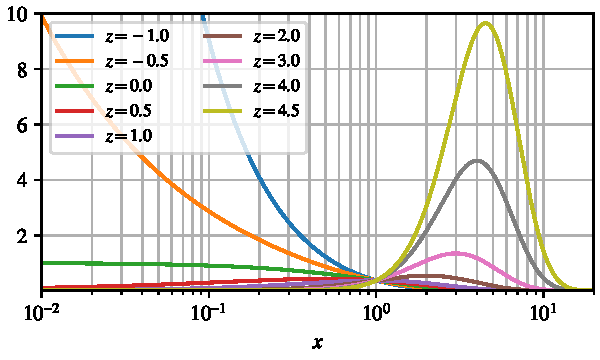
\includegraphics{papers/laguerre/images/integrand_exp.pdf}
%\vspace{-12pt}
\caption{Integrand $x^z e^{-x}$ mit unterschiedlichen Werten für $z$}
\label{laguerre:fig:integrand_exp}
\end{figure}

In Abbildung~\ref{laguerre:fig:integrand_exp} fügen wir
die Dämpfung der Gewichtsfunktion $w(x)$
der Gauss-Laguerre-Quadratur wieder hinzu
und erhalten so wieder den kompletten Integranden $x^{z-1} e^{-x}$
der Gamma-Funktion.
Für negative $z$ ergeben sich immer noch Singularitäten,
wenn $x \rightarrow 0$.
Um $1$ wächst der Term $x^z$ schneller als die Dämpfung $e^{-x}$,
aber für $x \rightarrow \infty$ geht der Integrand gegen $0$.
Das führt zu glockenförmigen Kurven,
die für grosse Exponenten $z$ nach der Stelle $x=1$ schnell anwachsen.
Zu grosse Exponenten $z$ sind also immer noch problematisch.
Kleine positive $z$ scheinen nun also auch zulässig zu sein.
Damit formulieren wir die Vermutung,
dass $a(n)$,
welches das Intervall $[a(n), a(n) + 1]$ definiert,
in dem der relative Fehler minimal ist,
grösser als $0$ und kleiner als $2n-1$ ist.

\subsubsection{Ansatz mit Verschiebungsterm}
% Mittels der Funktionalgleichung \eqref{laguerre:gamma_funktional} 
% kann der Wert von $\Gamma(z)$ im Interval $z \in [a,a+1]$,
% in dem der relative Fehler minimal ist,
% evaluiert werden und dann mit der Funktionalgleichung zurückverschoben werden.
Nun stellt sich die Frage,
ob die Approximation mittels Gauss-Laguerre-Quadratur verbessert werden kann,
wenn man das Problem in einem geeigneten Intervall $[a(n), a(n)+1]$,
$a(n) \in \mathbb{Z}$,
evaluiert und dann mit der
Funktionalgleichung \eqref{laguerre:gamma_funktional} zurückverschiebt.
Für dieses Vorhaben führen wir einen Verschiebungsterm $m \in \mathbb{Z}$ ein.
Passen wir \eqref{laguerre:naive_lag}
mit dem Verschiebungsterm $m$
%,der $z$ and die Stelle $z_m = z + m$ verschiebt, 
an,
ergibt sich
\begin{align}
\Gamma(z)
\approx
s(z, m) \sum_{i=1}^n x_i^{z + m - 1} A_i
% &&
% \text{mit }
% s(z, m)
% =
% \begin{cases}
% \displaystyle
% \frac{1}{(z - m)_m} & \text{wenn } m \geq 0\\
% (z + m)_{-m} & \text{wenn } m < 0
% \end{cases}
% .
\label{laguerre:shifted_lag}
\end{align}
mit
\begin{align*}
s(z, m)
=
\begin{cases}
\displaystyle
\frac{1}{(z)_m} & \text{wenn } m \geq 0 \\
(z + m)_{-m}    & \text{wenn } m < 0
\end{cases}
.
\end{align*}

\subsubsection{Finden der optimalen Berechnungsstelle}
Um die optimale Stelle $z^*(n) \in \left[a(n), a(n) + 1\right]$,
$z^*(n) \in \mathbb{R}$,
zu finden,
erweitern wir denn Fehlerterm \eqref{laguerre:gamma_err_simple}
und erhalten
\begin{align}
R_{n,m}(\xi)
=
s(z, m) \cdot (z - 2n)_{2n} \frac{(n!)^2}{(2n)!} \xi^{z + m - 2n - 1}
,\quad
\text{für }
\xi \in (0, \infty)
\label{laguerre:gamma_err_shifted}
.
\end{align}

\begin{figure}
\centering
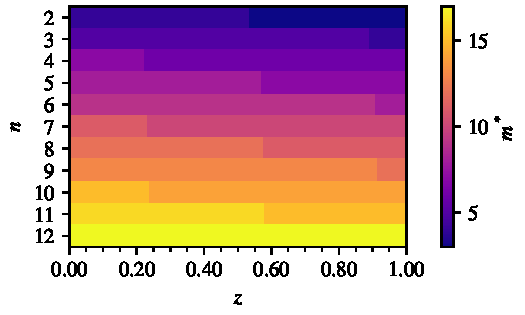
\includegraphics{papers/laguerre/images/targets.pdf}
% %\vspace{-12pt}
\caption{$a$ in Abhängigkeit von $z$ und $n$}
\label{laguerre:fig:targets}
\end{figure}
% wobei  ist
% mit $z^*(n) \in \mathbb{R}$ wollen wir finden,
% in dem wir den Fehlerterm \eqref{laguerre:lag_error} anpassen
% und in einem nächsten Schritt minimieren.
% Zudem nehmen wir an,
% dass $z < z^*(n)$ ist.
% Wir fügen einen Verschiebungsterm um $m \in \mathbb{N}$ Stellen ein,
% daraus folgt
%
% Damit wir den idealen Verschiebungsterm $m^*$ finden können,
% müssen wir mittels des Fehlerterms \eqref{laguerre:gamma_err_shifted}
% ein Optimierungsproblem
%
% Das Optimierungsproblem daraus lässt sich als
Daraus formulieren wir das Optimierungproblem
\begin{align*}
m^*
=
\operatorname*{argmin}_m \max_\xi R_{n,m}(\xi)
.
\end{align*}
Allerdings ist die Funktion $R_{n,m}(\xi)$ unbeschränkt und
hat die gleichen Probleme wie die Fehlerabschätzung des direkten Ansatzes.
Dazu müssten wir $\xi$ versuchen,
unter Kontrolle zu bringen,
was ein äussersts schwieriges Unterfangen zu sein scheint.
Da die Gauss-Quadratur aber sowieso
nur wirklich praktisch sinnvoll für kleine $n$ ist,
können die Intervalle $[a(n), a(n)+1]$ empirisch gesucht werden.

Wir bestimmen nun die optimalen Verschiebungsterme empirisch
für $n = 2,\ldots, 12$ im Intervall $z \in (0, 1)$,
da $z$ sowieso um den Term $m$ verschoben wird,
reicht die $m^*$ nur in diesem Intervall zu analysieren.
In Abbildung~\ref{laguerre:fig:targets} sind die empirisch bestimmten $m^*$
abhängig von $z$ und $n$ dargestellt.
In $n$-Richtung lässt sich eine klare lineare Abhängigkeit erkennen und
die Beziehung zu $z$ ist negativ,
d.h. wenn $z$ grösser ist, wird $m^*$ kleiner.
Allerdings ist die genaue Beziehung zu $z$
aus dieser Grafik nicht offensichtlich,
aber sie scheint regelmässig zu sein.
Es lässt die Vermutung aufkommen,
dass die Restriktion von $m^* \in \mathbb{Z}$ Rundungsprobleme verursacht.
Wir versuchen,
dieses Problem via lineare Regression und geeignete Rundung zu beheben.
Den linearen Regressor
\begin{align*}
\hat{m}
=
\alpha n + \beta
\end{align*}
machen wir nur abhängig von $n$
in dem wir den Mittelwert $\overline{m}$ von $m^*$ über $z$ berechnen.

\begin{figure}
\centering
% %% Creator: Matplotlib, PGF backend
%%
%% To include the figure in your LaTeX document, write
%%   \input{<filename>.pgf}
%%
%% Make sure the required packages are loaded in your preamble
%%   \usepackage{pgf}
%%
%% Also ensure that all the required font packages are loaded; for instance,
%% the lmodern package is sometimes necessary when using math font.
%%   \usepackage{lmodern}
%%
%% Figures using additional raster images can only be included by \input if
%% they are in the same directory as the main LaTeX file. For loading figures
%% from other directories you can use the `import` package
%%   \usepackage{import}
%%
%% and then include the figures with
%%   \import{<path to file>}{<filename>.pgf}
%%
%% Matplotlib used the following preamble
%%   \usepackage{fontspec}
%%   \setmainfont{DejaVuSerif.ttf}[Path=\detokenize{/home/mup/.local/lib/python3.8/site-packages/matplotlib/mpl-data/fonts/ttf/}]
%%   \setsansfont{DejaVuSans.ttf}[Path=\detokenize{/home/mup/.local/lib/python3.8/site-packages/matplotlib/mpl-data/fonts/ttf/}]
%%   \setmonofont{DejaVuSansMono.ttf}[Path=\detokenize{/home/mup/.local/lib/python3.8/site-packages/matplotlib/mpl-data/fonts/ttf/}]
%%
\begingroup%
\makeatletter%
\begin{pgfpicture}%
\pgfpathrectangle{\pgfpointorigin}{\pgfqpoint{4.500000in}{3.600000in}}%
\pgfusepath{use as bounding box, clip}%
\begin{pgfscope}%
\pgfsetbuttcap%
\pgfsetmiterjoin%
\definecolor{currentfill}{rgb}{1.000000,1.000000,1.000000}%
\pgfsetfillcolor{currentfill}%
\pgfsetlinewidth{0.000000pt}%
\definecolor{currentstroke}{rgb}{1.000000,1.000000,1.000000}%
\pgfsetstrokecolor{currentstroke}%
\pgfsetdash{}{0pt}%
\pgfpathmoveto{\pgfqpoint{0.000000in}{0.000000in}}%
\pgfpathlineto{\pgfqpoint{4.500000in}{0.000000in}}%
\pgfpathlineto{\pgfqpoint{4.500000in}{3.600000in}}%
\pgfpathlineto{\pgfqpoint{0.000000in}{3.600000in}}%
\pgfpathlineto{\pgfqpoint{0.000000in}{0.000000in}}%
\pgfpathclose%
\pgfusepath{fill}%
\end{pgfscope}%
\begin{pgfscope}%
\pgfsetbuttcap%
\pgfsetmiterjoin%
\definecolor{currentfill}{rgb}{1.000000,1.000000,1.000000}%
\pgfsetfillcolor{currentfill}%
\pgfsetlinewidth{0.000000pt}%
\definecolor{currentstroke}{rgb}{0.000000,0.000000,0.000000}%
\pgfsetstrokecolor{currentstroke}%
\pgfsetstrokeopacity{0.000000}%
\pgfsetdash{}{0pt}%
\pgfpathmoveto{\pgfqpoint{0.556162in}{2.076777in}}%
\pgfpathlineto{\pgfqpoint{4.458330in}{2.076777in}}%
\pgfpathlineto{\pgfqpoint{4.458330in}{3.558330in}}%
\pgfpathlineto{\pgfqpoint{0.556162in}{3.558330in}}%
\pgfpathlineto{\pgfqpoint{0.556162in}{2.076777in}}%
\pgfpathclose%
\pgfusepath{fill}%
\end{pgfscope}%
\begin{pgfscope}%
\pgfpathrectangle{\pgfqpoint{0.556162in}{2.076777in}}{\pgfqpoint{3.902168in}{1.481553in}}%
\pgfusepath{clip}%
\pgfsetrectcap%
\pgfsetroundjoin%
\pgfsetlinewidth{0.803000pt}%
\definecolor{currentstroke}{rgb}{0.690196,0.690196,0.690196}%
\pgfsetstrokecolor{currentstroke}%
\pgfsetdash{}{0pt}%
\pgfpathmoveto{\pgfqpoint{0.733533in}{2.076777in}}%
\pgfpathlineto{\pgfqpoint{0.733533in}{3.558330in}}%
\pgfusepath{stroke}%
\end{pgfscope}%
\begin{pgfscope}%
\pgfsetbuttcap%
\pgfsetroundjoin%
\definecolor{currentfill}{rgb}{0.000000,0.000000,0.000000}%
\pgfsetfillcolor{currentfill}%
\pgfsetlinewidth{0.803000pt}%
\definecolor{currentstroke}{rgb}{0.000000,0.000000,0.000000}%
\pgfsetstrokecolor{currentstroke}%
\pgfsetdash{}{0pt}%
\pgfsys@defobject{currentmarker}{\pgfqpoint{0.000000in}{-0.048611in}}{\pgfqpoint{0.000000in}{0.000000in}}{%
\pgfpathmoveto{\pgfqpoint{0.000000in}{0.000000in}}%
\pgfpathlineto{\pgfqpoint{0.000000in}{-0.048611in}}%
\pgfusepath{stroke,fill}%
}%
\begin{pgfscope}%
\pgfsys@transformshift{0.733533in}{2.076777in}%
\pgfsys@useobject{currentmarker}{}%
\end{pgfscope}%
\end{pgfscope}%
\begin{pgfscope}%
\pgfpathrectangle{\pgfqpoint{0.556162in}{2.076777in}}{\pgfqpoint{3.902168in}{1.481553in}}%
\pgfusepath{clip}%
\pgfsetrectcap%
\pgfsetroundjoin%
\pgfsetlinewidth{0.803000pt}%
\definecolor{currentstroke}{rgb}{0.690196,0.690196,0.690196}%
\pgfsetstrokecolor{currentstroke}%
\pgfsetdash{}{0pt}%
\pgfpathmoveto{\pgfqpoint{1.088276in}{2.076777in}}%
\pgfpathlineto{\pgfqpoint{1.088276in}{3.558330in}}%
\pgfusepath{stroke}%
\end{pgfscope}%
\begin{pgfscope}%
\pgfsetbuttcap%
\pgfsetroundjoin%
\definecolor{currentfill}{rgb}{0.000000,0.000000,0.000000}%
\pgfsetfillcolor{currentfill}%
\pgfsetlinewidth{0.803000pt}%
\definecolor{currentstroke}{rgb}{0.000000,0.000000,0.000000}%
\pgfsetstrokecolor{currentstroke}%
\pgfsetdash{}{0pt}%
\pgfsys@defobject{currentmarker}{\pgfqpoint{0.000000in}{-0.048611in}}{\pgfqpoint{0.000000in}{0.000000in}}{%
\pgfpathmoveto{\pgfqpoint{0.000000in}{0.000000in}}%
\pgfpathlineto{\pgfqpoint{0.000000in}{-0.048611in}}%
\pgfusepath{stroke,fill}%
}%
\begin{pgfscope}%
\pgfsys@transformshift{1.088276in}{2.076777in}%
\pgfsys@useobject{currentmarker}{}%
\end{pgfscope}%
\end{pgfscope}%
\begin{pgfscope}%
\pgfpathrectangle{\pgfqpoint{0.556162in}{2.076777in}}{\pgfqpoint{3.902168in}{1.481553in}}%
\pgfusepath{clip}%
\pgfsetrectcap%
\pgfsetroundjoin%
\pgfsetlinewidth{0.803000pt}%
\definecolor{currentstroke}{rgb}{0.690196,0.690196,0.690196}%
\pgfsetstrokecolor{currentstroke}%
\pgfsetdash{}{0pt}%
\pgfpathmoveto{\pgfqpoint{1.443018in}{2.076777in}}%
\pgfpathlineto{\pgfqpoint{1.443018in}{3.558330in}}%
\pgfusepath{stroke}%
\end{pgfscope}%
\begin{pgfscope}%
\pgfsetbuttcap%
\pgfsetroundjoin%
\definecolor{currentfill}{rgb}{0.000000,0.000000,0.000000}%
\pgfsetfillcolor{currentfill}%
\pgfsetlinewidth{0.803000pt}%
\definecolor{currentstroke}{rgb}{0.000000,0.000000,0.000000}%
\pgfsetstrokecolor{currentstroke}%
\pgfsetdash{}{0pt}%
\pgfsys@defobject{currentmarker}{\pgfqpoint{0.000000in}{-0.048611in}}{\pgfqpoint{0.000000in}{0.000000in}}{%
\pgfpathmoveto{\pgfqpoint{0.000000in}{0.000000in}}%
\pgfpathlineto{\pgfqpoint{0.000000in}{-0.048611in}}%
\pgfusepath{stroke,fill}%
}%
\begin{pgfscope}%
\pgfsys@transformshift{1.443018in}{2.076777in}%
\pgfsys@useobject{currentmarker}{}%
\end{pgfscope}%
\end{pgfscope}%
\begin{pgfscope}%
\pgfpathrectangle{\pgfqpoint{0.556162in}{2.076777in}}{\pgfqpoint{3.902168in}{1.481553in}}%
\pgfusepath{clip}%
\pgfsetrectcap%
\pgfsetroundjoin%
\pgfsetlinewidth{0.803000pt}%
\definecolor{currentstroke}{rgb}{0.690196,0.690196,0.690196}%
\pgfsetstrokecolor{currentstroke}%
\pgfsetdash{}{0pt}%
\pgfpathmoveto{\pgfqpoint{1.797761in}{2.076777in}}%
\pgfpathlineto{\pgfqpoint{1.797761in}{3.558330in}}%
\pgfusepath{stroke}%
\end{pgfscope}%
\begin{pgfscope}%
\pgfsetbuttcap%
\pgfsetroundjoin%
\definecolor{currentfill}{rgb}{0.000000,0.000000,0.000000}%
\pgfsetfillcolor{currentfill}%
\pgfsetlinewidth{0.803000pt}%
\definecolor{currentstroke}{rgb}{0.000000,0.000000,0.000000}%
\pgfsetstrokecolor{currentstroke}%
\pgfsetdash{}{0pt}%
\pgfsys@defobject{currentmarker}{\pgfqpoint{0.000000in}{-0.048611in}}{\pgfqpoint{0.000000in}{0.000000in}}{%
\pgfpathmoveto{\pgfqpoint{0.000000in}{0.000000in}}%
\pgfpathlineto{\pgfqpoint{0.000000in}{-0.048611in}}%
\pgfusepath{stroke,fill}%
}%
\begin{pgfscope}%
\pgfsys@transformshift{1.797761in}{2.076777in}%
\pgfsys@useobject{currentmarker}{}%
\end{pgfscope}%
\end{pgfscope}%
\begin{pgfscope}%
\pgfpathrectangle{\pgfqpoint{0.556162in}{2.076777in}}{\pgfqpoint{3.902168in}{1.481553in}}%
\pgfusepath{clip}%
\pgfsetrectcap%
\pgfsetroundjoin%
\pgfsetlinewidth{0.803000pt}%
\definecolor{currentstroke}{rgb}{0.690196,0.690196,0.690196}%
\pgfsetstrokecolor{currentstroke}%
\pgfsetdash{}{0pt}%
\pgfpathmoveto{\pgfqpoint{2.152504in}{2.076777in}}%
\pgfpathlineto{\pgfqpoint{2.152504in}{3.558330in}}%
\pgfusepath{stroke}%
\end{pgfscope}%
\begin{pgfscope}%
\pgfsetbuttcap%
\pgfsetroundjoin%
\definecolor{currentfill}{rgb}{0.000000,0.000000,0.000000}%
\pgfsetfillcolor{currentfill}%
\pgfsetlinewidth{0.803000pt}%
\definecolor{currentstroke}{rgb}{0.000000,0.000000,0.000000}%
\pgfsetstrokecolor{currentstroke}%
\pgfsetdash{}{0pt}%
\pgfsys@defobject{currentmarker}{\pgfqpoint{0.000000in}{-0.048611in}}{\pgfqpoint{0.000000in}{0.000000in}}{%
\pgfpathmoveto{\pgfqpoint{0.000000in}{0.000000in}}%
\pgfpathlineto{\pgfqpoint{0.000000in}{-0.048611in}}%
\pgfusepath{stroke,fill}%
}%
\begin{pgfscope}%
\pgfsys@transformshift{2.152504in}{2.076777in}%
\pgfsys@useobject{currentmarker}{}%
\end{pgfscope}%
\end{pgfscope}%
\begin{pgfscope}%
\pgfpathrectangle{\pgfqpoint{0.556162in}{2.076777in}}{\pgfqpoint{3.902168in}{1.481553in}}%
\pgfusepath{clip}%
\pgfsetrectcap%
\pgfsetroundjoin%
\pgfsetlinewidth{0.803000pt}%
\definecolor{currentstroke}{rgb}{0.690196,0.690196,0.690196}%
\pgfsetstrokecolor{currentstroke}%
\pgfsetdash{}{0pt}%
\pgfpathmoveto{\pgfqpoint{2.507246in}{2.076777in}}%
\pgfpathlineto{\pgfqpoint{2.507246in}{3.558330in}}%
\pgfusepath{stroke}%
\end{pgfscope}%
\begin{pgfscope}%
\pgfsetbuttcap%
\pgfsetroundjoin%
\definecolor{currentfill}{rgb}{0.000000,0.000000,0.000000}%
\pgfsetfillcolor{currentfill}%
\pgfsetlinewidth{0.803000pt}%
\definecolor{currentstroke}{rgb}{0.000000,0.000000,0.000000}%
\pgfsetstrokecolor{currentstroke}%
\pgfsetdash{}{0pt}%
\pgfsys@defobject{currentmarker}{\pgfqpoint{0.000000in}{-0.048611in}}{\pgfqpoint{0.000000in}{0.000000in}}{%
\pgfpathmoveto{\pgfqpoint{0.000000in}{0.000000in}}%
\pgfpathlineto{\pgfqpoint{0.000000in}{-0.048611in}}%
\pgfusepath{stroke,fill}%
}%
\begin{pgfscope}%
\pgfsys@transformshift{2.507246in}{2.076777in}%
\pgfsys@useobject{currentmarker}{}%
\end{pgfscope}%
\end{pgfscope}%
\begin{pgfscope}%
\pgfpathrectangle{\pgfqpoint{0.556162in}{2.076777in}}{\pgfqpoint{3.902168in}{1.481553in}}%
\pgfusepath{clip}%
\pgfsetrectcap%
\pgfsetroundjoin%
\pgfsetlinewidth{0.803000pt}%
\definecolor{currentstroke}{rgb}{0.690196,0.690196,0.690196}%
\pgfsetstrokecolor{currentstroke}%
\pgfsetdash{}{0pt}%
\pgfpathmoveto{\pgfqpoint{2.861989in}{2.076777in}}%
\pgfpathlineto{\pgfqpoint{2.861989in}{3.558330in}}%
\pgfusepath{stroke}%
\end{pgfscope}%
\begin{pgfscope}%
\pgfsetbuttcap%
\pgfsetroundjoin%
\definecolor{currentfill}{rgb}{0.000000,0.000000,0.000000}%
\pgfsetfillcolor{currentfill}%
\pgfsetlinewidth{0.803000pt}%
\definecolor{currentstroke}{rgb}{0.000000,0.000000,0.000000}%
\pgfsetstrokecolor{currentstroke}%
\pgfsetdash{}{0pt}%
\pgfsys@defobject{currentmarker}{\pgfqpoint{0.000000in}{-0.048611in}}{\pgfqpoint{0.000000in}{0.000000in}}{%
\pgfpathmoveto{\pgfqpoint{0.000000in}{0.000000in}}%
\pgfpathlineto{\pgfqpoint{0.000000in}{-0.048611in}}%
\pgfusepath{stroke,fill}%
}%
\begin{pgfscope}%
\pgfsys@transformshift{2.861989in}{2.076777in}%
\pgfsys@useobject{currentmarker}{}%
\end{pgfscope}%
\end{pgfscope}%
\begin{pgfscope}%
\pgfpathrectangle{\pgfqpoint{0.556162in}{2.076777in}}{\pgfqpoint{3.902168in}{1.481553in}}%
\pgfusepath{clip}%
\pgfsetrectcap%
\pgfsetroundjoin%
\pgfsetlinewidth{0.803000pt}%
\definecolor{currentstroke}{rgb}{0.690196,0.690196,0.690196}%
\pgfsetstrokecolor{currentstroke}%
\pgfsetdash{}{0pt}%
\pgfpathmoveto{\pgfqpoint{3.216731in}{2.076777in}}%
\pgfpathlineto{\pgfqpoint{3.216731in}{3.558330in}}%
\pgfusepath{stroke}%
\end{pgfscope}%
\begin{pgfscope}%
\pgfsetbuttcap%
\pgfsetroundjoin%
\definecolor{currentfill}{rgb}{0.000000,0.000000,0.000000}%
\pgfsetfillcolor{currentfill}%
\pgfsetlinewidth{0.803000pt}%
\definecolor{currentstroke}{rgb}{0.000000,0.000000,0.000000}%
\pgfsetstrokecolor{currentstroke}%
\pgfsetdash{}{0pt}%
\pgfsys@defobject{currentmarker}{\pgfqpoint{0.000000in}{-0.048611in}}{\pgfqpoint{0.000000in}{0.000000in}}{%
\pgfpathmoveto{\pgfqpoint{0.000000in}{0.000000in}}%
\pgfpathlineto{\pgfqpoint{0.000000in}{-0.048611in}}%
\pgfusepath{stroke,fill}%
}%
\begin{pgfscope}%
\pgfsys@transformshift{3.216731in}{2.076777in}%
\pgfsys@useobject{currentmarker}{}%
\end{pgfscope}%
\end{pgfscope}%
\begin{pgfscope}%
\pgfpathrectangle{\pgfqpoint{0.556162in}{2.076777in}}{\pgfqpoint{3.902168in}{1.481553in}}%
\pgfusepath{clip}%
\pgfsetrectcap%
\pgfsetroundjoin%
\pgfsetlinewidth{0.803000pt}%
\definecolor{currentstroke}{rgb}{0.690196,0.690196,0.690196}%
\pgfsetstrokecolor{currentstroke}%
\pgfsetdash{}{0pt}%
\pgfpathmoveto{\pgfqpoint{3.571474in}{2.076777in}}%
\pgfpathlineto{\pgfqpoint{3.571474in}{3.558330in}}%
\pgfusepath{stroke}%
\end{pgfscope}%
\begin{pgfscope}%
\pgfsetbuttcap%
\pgfsetroundjoin%
\definecolor{currentfill}{rgb}{0.000000,0.000000,0.000000}%
\pgfsetfillcolor{currentfill}%
\pgfsetlinewidth{0.803000pt}%
\definecolor{currentstroke}{rgb}{0.000000,0.000000,0.000000}%
\pgfsetstrokecolor{currentstroke}%
\pgfsetdash{}{0pt}%
\pgfsys@defobject{currentmarker}{\pgfqpoint{0.000000in}{-0.048611in}}{\pgfqpoint{0.000000in}{0.000000in}}{%
\pgfpathmoveto{\pgfqpoint{0.000000in}{0.000000in}}%
\pgfpathlineto{\pgfqpoint{0.000000in}{-0.048611in}}%
\pgfusepath{stroke,fill}%
}%
\begin{pgfscope}%
\pgfsys@transformshift{3.571474in}{2.076777in}%
\pgfsys@useobject{currentmarker}{}%
\end{pgfscope}%
\end{pgfscope}%
\begin{pgfscope}%
\pgfpathrectangle{\pgfqpoint{0.556162in}{2.076777in}}{\pgfqpoint{3.902168in}{1.481553in}}%
\pgfusepath{clip}%
\pgfsetrectcap%
\pgfsetroundjoin%
\pgfsetlinewidth{0.803000pt}%
\definecolor{currentstroke}{rgb}{0.690196,0.690196,0.690196}%
\pgfsetstrokecolor{currentstroke}%
\pgfsetdash{}{0pt}%
\pgfpathmoveto{\pgfqpoint{3.926216in}{2.076777in}}%
\pgfpathlineto{\pgfqpoint{3.926216in}{3.558330in}}%
\pgfusepath{stroke}%
\end{pgfscope}%
\begin{pgfscope}%
\pgfsetbuttcap%
\pgfsetroundjoin%
\definecolor{currentfill}{rgb}{0.000000,0.000000,0.000000}%
\pgfsetfillcolor{currentfill}%
\pgfsetlinewidth{0.803000pt}%
\definecolor{currentstroke}{rgb}{0.000000,0.000000,0.000000}%
\pgfsetstrokecolor{currentstroke}%
\pgfsetdash{}{0pt}%
\pgfsys@defobject{currentmarker}{\pgfqpoint{0.000000in}{-0.048611in}}{\pgfqpoint{0.000000in}{0.000000in}}{%
\pgfpathmoveto{\pgfqpoint{0.000000in}{0.000000in}}%
\pgfpathlineto{\pgfqpoint{0.000000in}{-0.048611in}}%
\pgfusepath{stroke,fill}%
}%
\begin{pgfscope}%
\pgfsys@transformshift{3.926216in}{2.076777in}%
\pgfsys@useobject{currentmarker}{}%
\end{pgfscope}%
\end{pgfscope}%
\begin{pgfscope}%
\pgfpathrectangle{\pgfqpoint{0.556162in}{2.076777in}}{\pgfqpoint{3.902168in}{1.481553in}}%
\pgfusepath{clip}%
\pgfsetrectcap%
\pgfsetroundjoin%
\pgfsetlinewidth{0.803000pt}%
\definecolor{currentstroke}{rgb}{0.690196,0.690196,0.690196}%
\pgfsetstrokecolor{currentstroke}%
\pgfsetdash{}{0pt}%
\pgfpathmoveto{\pgfqpoint{4.280959in}{2.076777in}}%
\pgfpathlineto{\pgfqpoint{4.280959in}{3.558330in}}%
\pgfusepath{stroke}%
\end{pgfscope}%
\begin{pgfscope}%
\pgfsetbuttcap%
\pgfsetroundjoin%
\definecolor{currentfill}{rgb}{0.000000,0.000000,0.000000}%
\pgfsetfillcolor{currentfill}%
\pgfsetlinewidth{0.803000pt}%
\definecolor{currentstroke}{rgb}{0.000000,0.000000,0.000000}%
\pgfsetstrokecolor{currentstroke}%
\pgfsetdash{}{0pt}%
\pgfsys@defobject{currentmarker}{\pgfqpoint{0.000000in}{-0.048611in}}{\pgfqpoint{0.000000in}{0.000000in}}{%
\pgfpathmoveto{\pgfqpoint{0.000000in}{0.000000in}}%
\pgfpathlineto{\pgfqpoint{0.000000in}{-0.048611in}}%
\pgfusepath{stroke,fill}%
}%
\begin{pgfscope}%
\pgfsys@transformshift{4.280959in}{2.076777in}%
\pgfsys@useobject{currentmarker}{}%
\end{pgfscope}%
\end{pgfscope}%
\begin{pgfscope}%
\pgfpathrectangle{\pgfqpoint{0.556162in}{2.076777in}}{\pgfqpoint{3.902168in}{1.481553in}}%
\pgfusepath{clip}%
\pgfsetrectcap%
\pgfsetroundjoin%
\pgfsetlinewidth{0.803000pt}%
\definecolor{currentstroke}{rgb}{0.690196,0.690196,0.690196}%
\pgfsetstrokecolor{currentstroke}%
\pgfsetdash{}{0pt}%
\pgfpathmoveto{\pgfqpoint{0.556162in}{2.156403in}}%
\pgfpathlineto{\pgfqpoint{4.458330in}{2.156403in}}%
\pgfusepath{stroke}%
\end{pgfscope}%
\begin{pgfscope}%
\pgfsetbuttcap%
\pgfsetroundjoin%
\definecolor{currentfill}{rgb}{0.000000,0.000000,0.000000}%
\pgfsetfillcolor{currentfill}%
\pgfsetlinewidth{0.803000pt}%
\definecolor{currentstroke}{rgb}{0.000000,0.000000,0.000000}%
\pgfsetstrokecolor{currentstroke}%
\pgfsetdash{}{0pt}%
\pgfsys@defobject{currentmarker}{\pgfqpoint{-0.048611in}{0.000000in}}{\pgfqpoint{-0.000000in}{0.000000in}}{%
\pgfpathmoveto{\pgfqpoint{-0.000000in}{0.000000in}}%
\pgfpathlineto{\pgfqpoint{-0.048611in}{0.000000in}}%
\pgfusepath{stroke,fill}%
}%
\begin{pgfscope}%
\pgfsys@transformshift{0.556162in}{2.156403in}%
\pgfsys@useobject{currentmarker}{}%
\end{pgfscope}%
\end{pgfscope}%
\begin{pgfscope}%
\definecolor{textcolor}{rgb}{0.000000,0.000000,0.000000}%
\pgfsetstrokecolor{textcolor}%
\pgfsetfillcolor{textcolor}%
\pgftext[x=0.370575in, y=2.103641in, left, base]{\color{textcolor}\sffamily\fontsize{10.000000}{12.000000}\selectfont 3}%
\end{pgfscope}%
\begin{pgfscope}%
\pgfpathrectangle{\pgfqpoint{0.556162in}{2.076777in}}{\pgfqpoint{3.902168in}{1.481553in}}%
\pgfusepath{clip}%
\pgfsetrectcap%
\pgfsetroundjoin%
\pgfsetlinewidth{0.803000pt}%
\definecolor{currentstroke}{rgb}{0.690196,0.690196,0.690196}%
\pgfsetstrokecolor{currentstroke}%
\pgfsetdash{}{0pt}%
\pgfpathmoveto{\pgfqpoint{0.556162in}{2.339026in}}%
\pgfpathlineto{\pgfqpoint{4.458330in}{2.339026in}}%
\pgfusepath{stroke}%
\end{pgfscope}%
\begin{pgfscope}%
\pgfsetbuttcap%
\pgfsetroundjoin%
\definecolor{currentfill}{rgb}{0.000000,0.000000,0.000000}%
\pgfsetfillcolor{currentfill}%
\pgfsetlinewidth{0.803000pt}%
\definecolor{currentstroke}{rgb}{0.000000,0.000000,0.000000}%
\pgfsetstrokecolor{currentstroke}%
\pgfsetdash{}{0pt}%
\pgfsys@defobject{currentmarker}{\pgfqpoint{-0.048611in}{0.000000in}}{\pgfqpoint{-0.000000in}{0.000000in}}{%
\pgfpathmoveto{\pgfqpoint{-0.000000in}{0.000000in}}%
\pgfpathlineto{\pgfqpoint{-0.048611in}{0.000000in}}%
\pgfusepath{stroke,fill}%
}%
\begin{pgfscope}%
\pgfsys@transformshift{0.556162in}{2.339026in}%
\pgfsys@useobject{currentmarker}{}%
\end{pgfscope}%
\end{pgfscope}%
\begin{pgfscope}%
\definecolor{textcolor}{rgb}{0.000000,0.000000,0.000000}%
\pgfsetstrokecolor{textcolor}%
\pgfsetfillcolor{textcolor}%
\pgftext[x=0.370575in, y=2.286264in, left, base]{\color{textcolor}\sffamily\fontsize{10.000000}{12.000000}\selectfont 5}%
\end{pgfscope}%
\begin{pgfscope}%
\pgfpathrectangle{\pgfqpoint{0.556162in}{2.076777in}}{\pgfqpoint{3.902168in}{1.481553in}}%
\pgfusepath{clip}%
\pgfsetrectcap%
\pgfsetroundjoin%
\pgfsetlinewidth{0.803000pt}%
\definecolor{currentstroke}{rgb}{0.690196,0.690196,0.690196}%
\pgfsetstrokecolor{currentstroke}%
\pgfsetdash{}{0pt}%
\pgfpathmoveto{\pgfqpoint{0.556162in}{2.521648in}}%
\pgfpathlineto{\pgfqpoint{4.458330in}{2.521648in}}%
\pgfusepath{stroke}%
\end{pgfscope}%
\begin{pgfscope}%
\pgfsetbuttcap%
\pgfsetroundjoin%
\definecolor{currentfill}{rgb}{0.000000,0.000000,0.000000}%
\pgfsetfillcolor{currentfill}%
\pgfsetlinewidth{0.803000pt}%
\definecolor{currentstroke}{rgb}{0.000000,0.000000,0.000000}%
\pgfsetstrokecolor{currentstroke}%
\pgfsetdash{}{0pt}%
\pgfsys@defobject{currentmarker}{\pgfqpoint{-0.048611in}{0.000000in}}{\pgfqpoint{-0.000000in}{0.000000in}}{%
\pgfpathmoveto{\pgfqpoint{-0.000000in}{0.000000in}}%
\pgfpathlineto{\pgfqpoint{-0.048611in}{0.000000in}}%
\pgfusepath{stroke,fill}%
}%
\begin{pgfscope}%
\pgfsys@transformshift{0.556162in}{2.521648in}%
\pgfsys@useobject{currentmarker}{}%
\end{pgfscope}%
\end{pgfscope}%
\begin{pgfscope}%
\definecolor{textcolor}{rgb}{0.000000,0.000000,0.000000}%
\pgfsetstrokecolor{textcolor}%
\pgfsetfillcolor{textcolor}%
\pgftext[x=0.370575in, y=2.468887in, left, base]{\color{textcolor}\sffamily\fontsize{10.000000}{12.000000}\selectfont 7}%
\end{pgfscope}%
\begin{pgfscope}%
\pgfpathrectangle{\pgfqpoint{0.556162in}{2.076777in}}{\pgfqpoint{3.902168in}{1.481553in}}%
\pgfusepath{clip}%
\pgfsetrectcap%
\pgfsetroundjoin%
\pgfsetlinewidth{0.803000pt}%
\definecolor{currentstroke}{rgb}{0.690196,0.690196,0.690196}%
\pgfsetstrokecolor{currentstroke}%
\pgfsetdash{}{0pt}%
\pgfpathmoveto{\pgfqpoint{0.556162in}{2.704271in}}%
\pgfpathlineto{\pgfqpoint{4.458330in}{2.704271in}}%
\pgfusepath{stroke}%
\end{pgfscope}%
\begin{pgfscope}%
\pgfsetbuttcap%
\pgfsetroundjoin%
\definecolor{currentfill}{rgb}{0.000000,0.000000,0.000000}%
\pgfsetfillcolor{currentfill}%
\pgfsetlinewidth{0.803000pt}%
\definecolor{currentstroke}{rgb}{0.000000,0.000000,0.000000}%
\pgfsetstrokecolor{currentstroke}%
\pgfsetdash{}{0pt}%
\pgfsys@defobject{currentmarker}{\pgfqpoint{-0.048611in}{0.000000in}}{\pgfqpoint{-0.000000in}{0.000000in}}{%
\pgfpathmoveto{\pgfqpoint{-0.000000in}{0.000000in}}%
\pgfpathlineto{\pgfqpoint{-0.048611in}{0.000000in}}%
\pgfusepath{stroke,fill}%
}%
\begin{pgfscope}%
\pgfsys@transformshift{0.556162in}{2.704271in}%
\pgfsys@useobject{currentmarker}{}%
\end{pgfscope}%
\end{pgfscope}%
\begin{pgfscope}%
\definecolor{textcolor}{rgb}{0.000000,0.000000,0.000000}%
\pgfsetstrokecolor{textcolor}%
\pgfsetfillcolor{textcolor}%
\pgftext[x=0.370575in, y=2.651510in, left, base]{\color{textcolor}\sffamily\fontsize{10.000000}{12.000000}\selectfont 9}%
\end{pgfscope}%
\begin{pgfscope}%
\pgfpathrectangle{\pgfqpoint{0.556162in}{2.076777in}}{\pgfqpoint{3.902168in}{1.481553in}}%
\pgfusepath{clip}%
\pgfsetrectcap%
\pgfsetroundjoin%
\pgfsetlinewidth{0.803000pt}%
\definecolor{currentstroke}{rgb}{0.690196,0.690196,0.690196}%
\pgfsetstrokecolor{currentstroke}%
\pgfsetdash{}{0pt}%
\pgfpathmoveto{\pgfqpoint{0.556162in}{2.886894in}}%
\pgfpathlineto{\pgfqpoint{4.458330in}{2.886894in}}%
\pgfusepath{stroke}%
\end{pgfscope}%
\begin{pgfscope}%
\pgfsetbuttcap%
\pgfsetroundjoin%
\definecolor{currentfill}{rgb}{0.000000,0.000000,0.000000}%
\pgfsetfillcolor{currentfill}%
\pgfsetlinewidth{0.803000pt}%
\definecolor{currentstroke}{rgb}{0.000000,0.000000,0.000000}%
\pgfsetstrokecolor{currentstroke}%
\pgfsetdash{}{0pt}%
\pgfsys@defobject{currentmarker}{\pgfqpoint{-0.048611in}{0.000000in}}{\pgfqpoint{-0.000000in}{0.000000in}}{%
\pgfpathmoveto{\pgfqpoint{-0.000000in}{0.000000in}}%
\pgfpathlineto{\pgfqpoint{-0.048611in}{0.000000in}}%
\pgfusepath{stroke,fill}%
}%
\begin{pgfscope}%
\pgfsys@transformshift{0.556162in}{2.886894in}%
\pgfsys@useobject{currentmarker}{}%
\end{pgfscope}%
\end{pgfscope}%
\begin{pgfscope}%
\definecolor{textcolor}{rgb}{0.000000,0.000000,0.000000}%
\pgfsetstrokecolor{textcolor}%
\pgfsetfillcolor{textcolor}%
\pgftext[x=0.282209in, y=2.834133in, left, base]{\color{textcolor}\sffamily\fontsize{10.000000}{12.000000}\selectfont 11}%
\end{pgfscope}%
\begin{pgfscope}%
\pgfpathrectangle{\pgfqpoint{0.556162in}{2.076777in}}{\pgfqpoint{3.902168in}{1.481553in}}%
\pgfusepath{clip}%
\pgfsetrectcap%
\pgfsetroundjoin%
\pgfsetlinewidth{0.803000pt}%
\definecolor{currentstroke}{rgb}{0.690196,0.690196,0.690196}%
\pgfsetstrokecolor{currentstroke}%
\pgfsetdash{}{0pt}%
\pgfpathmoveto{\pgfqpoint{0.556162in}{3.069517in}}%
\pgfpathlineto{\pgfqpoint{4.458330in}{3.069517in}}%
\pgfusepath{stroke}%
\end{pgfscope}%
\begin{pgfscope}%
\pgfsetbuttcap%
\pgfsetroundjoin%
\definecolor{currentfill}{rgb}{0.000000,0.000000,0.000000}%
\pgfsetfillcolor{currentfill}%
\pgfsetlinewidth{0.803000pt}%
\definecolor{currentstroke}{rgb}{0.000000,0.000000,0.000000}%
\pgfsetstrokecolor{currentstroke}%
\pgfsetdash{}{0pt}%
\pgfsys@defobject{currentmarker}{\pgfqpoint{-0.048611in}{0.000000in}}{\pgfqpoint{-0.000000in}{0.000000in}}{%
\pgfpathmoveto{\pgfqpoint{-0.000000in}{0.000000in}}%
\pgfpathlineto{\pgfqpoint{-0.048611in}{0.000000in}}%
\pgfusepath{stroke,fill}%
}%
\begin{pgfscope}%
\pgfsys@transformshift{0.556162in}{3.069517in}%
\pgfsys@useobject{currentmarker}{}%
\end{pgfscope}%
\end{pgfscope}%
\begin{pgfscope}%
\definecolor{textcolor}{rgb}{0.000000,0.000000,0.000000}%
\pgfsetstrokecolor{textcolor}%
\pgfsetfillcolor{textcolor}%
\pgftext[x=0.282209in, y=3.016755in, left, base]{\color{textcolor}\sffamily\fontsize{10.000000}{12.000000}\selectfont 13}%
\end{pgfscope}%
\begin{pgfscope}%
\pgfpathrectangle{\pgfqpoint{0.556162in}{2.076777in}}{\pgfqpoint{3.902168in}{1.481553in}}%
\pgfusepath{clip}%
\pgfsetrectcap%
\pgfsetroundjoin%
\pgfsetlinewidth{0.803000pt}%
\definecolor{currentstroke}{rgb}{0.690196,0.690196,0.690196}%
\pgfsetstrokecolor{currentstroke}%
\pgfsetdash{}{0pt}%
\pgfpathmoveto{\pgfqpoint{0.556162in}{3.252140in}}%
\pgfpathlineto{\pgfqpoint{4.458330in}{3.252140in}}%
\pgfusepath{stroke}%
\end{pgfscope}%
\begin{pgfscope}%
\pgfsetbuttcap%
\pgfsetroundjoin%
\definecolor{currentfill}{rgb}{0.000000,0.000000,0.000000}%
\pgfsetfillcolor{currentfill}%
\pgfsetlinewidth{0.803000pt}%
\definecolor{currentstroke}{rgb}{0.000000,0.000000,0.000000}%
\pgfsetstrokecolor{currentstroke}%
\pgfsetdash{}{0pt}%
\pgfsys@defobject{currentmarker}{\pgfqpoint{-0.048611in}{0.000000in}}{\pgfqpoint{-0.000000in}{0.000000in}}{%
\pgfpathmoveto{\pgfqpoint{-0.000000in}{0.000000in}}%
\pgfpathlineto{\pgfqpoint{-0.048611in}{0.000000in}}%
\pgfusepath{stroke,fill}%
}%
\begin{pgfscope}%
\pgfsys@transformshift{0.556162in}{3.252140in}%
\pgfsys@useobject{currentmarker}{}%
\end{pgfscope}%
\end{pgfscope}%
\begin{pgfscope}%
\definecolor{textcolor}{rgb}{0.000000,0.000000,0.000000}%
\pgfsetstrokecolor{textcolor}%
\pgfsetfillcolor{textcolor}%
\pgftext[x=0.282209in, y=3.199378in, left, base]{\color{textcolor}\sffamily\fontsize{10.000000}{12.000000}\selectfont 15}%
\end{pgfscope}%
\begin{pgfscope}%
\pgfpathrectangle{\pgfqpoint{0.556162in}{2.076777in}}{\pgfqpoint{3.902168in}{1.481553in}}%
\pgfusepath{clip}%
\pgfsetrectcap%
\pgfsetroundjoin%
\pgfsetlinewidth{0.803000pt}%
\definecolor{currentstroke}{rgb}{0.690196,0.690196,0.690196}%
\pgfsetstrokecolor{currentstroke}%
\pgfsetdash{}{0pt}%
\pgfpathmoveto{\pgfqpoint{0.556162in}{3.434763in}}%
\pgfpathlineto{\pgfqpoint{4.458330in}{3.434763in}}%
\pgfusepath{stroke}%
\end{pgfscope}%
\begin{pgfscope}%
\pgfsetbuttcap%
\pgfsetroundjoin%
\definecolor{currentfill}{rgb}{0.000000,0.000000,0.000000}%
\pgfsetfillcolor{currentfill}%
\pgfsetlinewidth{0.803000pt}%
\definecolor{currentstroke}{rgb}{0.000000,0.000000,0.000000}%
\pgfsetstrokecolor{currentstroke}%
\pgfsetdash{}{0pt}%
\pgfsys@defobject{currentmarker}{\pgfqpoint{-0.048611in}{0.000000in}}{\pgfqpoint{-0.000000in}{0.000000in}}{%
\pgfpathmoveto{\pgfqpoint{-0.000000in}{0.000000in}}%
\pgfpathlineto{\pgfqpoint{-0.048611in}{0.000000in}}%
\pgfusepath{stroke,fill}%
}%
\begin{pgfscope}%
\pgfsys@transformshift{0.556162in}{3.434763in}%
\pgfsys@useobject{currentmarker}{}%
\end{pgfscope}%
\end{pgfscope}%
\begin{pgfscope}%
\definecolor{textcolor}{rgb}{0.000000,0.000000,0.000000}%
\pgfsetstrokecolor{textcolor}%
\pgfsetfillcolor{textcolor}%
\pgftext[x=0.282209in, y=3.382001in, left, base]{\color{textcolor}\sffamily\fontsize{10.000000}{12.000000}\selectfont 17}%
\end{pgfscope}%
\begin{pgfscope}%
\pgfpathrectangle{\pgfqpoint{0.556162in}{2.076777in}}{\pgfqpoint{3.902168in}{1.481553in}}%
\pgfusepath{clip}%
\pgfsetrectcap%
\pgfsetroundjoin%
\pgfsetlinewidth{1.505625pt}%
\definecolor{currentstroke}{rgb}{0.121569,0.466667,0.705882}%
\pgfsetstrokecolor{currentstroke}%
\pgfsetdash{}{0pt}%
\pgfpathmoveto{\pgfqpoint{0.556162in}{2.144121in}}%
\pgfpathlineto{\pgfqpoint{4.458330in}{3.490987in}}%
\pgfusepath{stroke}%
\end{pgfscope}%
\begin{pgfscope}%
\pgfpathrectangle{\pgfqpoint{0.556162in}{2.076777in}}{\pgfqpoint{3.902168in}{1.481553in}}%
\pgfusepath{clip}%
\pgfsetbuttcap%
\pgfsetroundjoin%
\definecolor{currentfill}{rgb}{1.000000,0.498039,0.054902}%
\pgfsetfillcolor{currentfill}%
\pgfsetlinewidth{1.003750pt}%
\definecolor{currentstroke}{rgb}{1.000000,0.498039,0.054902}%
\pgfsetstrokecolor{currentstroke}%
\pgfsetdash{}{0pt}%
\pgfsys@defobject{currentmarker}{\pgfqpoint{-0.041667in}{-0.041667in}}{\pgfqpoint{0.041667in}{0.041667in}}{%
\pgfpathmoveto{\pgfqpoint{-0.041667in}{-0.041667in}}%
\pgfpathlineto{\pgfqpoint{0.041667in}{0.041667in}}%
\pgfpathmoveto{\pgfqpoint{-0.041667in}{0.041667in}}%
\pgfpathlineto{\pgfqpoint{0.041667in}{-0.041667in}}%
\pgfusepath{stroke,fill}%
}%
\begin{pgfscope}%
\pgfsys@transformshift{0.733533in}{2.205011in}%
\pgfsys@useobject{currentmarker}{}%
\end{pgfscope}%
\begin{pgfscope}%
\pgfsys@transformshift{1.088276in}{2.328577in}%
\pgfsys@useobject{currentmarker}{}%
\end{pgfscope}%
\begin{pgfscope}%
\pgfsys@transformshift{1.443018in}{2.450780in}%
\pgfsys@useobject{currentmarker}{}%
\end{pgfscope}%
\begin{pgfscope}%
\pgfsys@transformshift{1.797761in}{2.573437in}%
\pgfsys@useobject{currentmarker}{}%
\end{pgfscope}%
\begin{pgfscope}%
\pgfsys@transformshift{2.152504in}{2.695640in}%
\pgfsys@useobject{currentmarker}{}%
\end{pgfscope}%
\begin{pgfscope}%
\pgfsys@transformshift{2.507246in}{2.816934in}%
\pgfsys@useobject{currentmarker}{}%
\end{pgfscope}%
\begin{pgfscope}%
\pgfsys@transformshift{2.861989in}{2.939137in}%
\pgfsys@useobject{currentmarker}{}%
\end{pgfscope}%
\begin{pgfscope}%
\pgfsys@transformshift{3.216731in}{3.061340in}%
\pgfsys@useobject{currentmarker}{}%
\end{pgfscope}%
\begin{pgfscope}%
\pgfsys@transformshift{3.571474in}{3.182634in}%
\pgfsys@useobject{currentmarker}{}%
\end{pgfscope}%
\begin{pgfscope}%
\pgfsys@transformshift{3.926216in}{3.304837in}%
\pgfsys@useobject{currentmarker}{}%
\end{pgfscope}%
\begin{pgfscope}%
\pgfsys@transformshift{4.280959in}{3.434763in}%
\pgfsys@useobject{currentmarker}{}%
\end{pgfscope}%
\end{pgfscope}%
\begin{pgfscope}%
\pgfsetrectcap%
\pgfsetmiterjoin%
\pgfsetlinewidth{0.803000pt}%
\definecolor{currentstroke}{rgb}{0.000000,0.000000,0.000000}%
\pgfsetstrokecolor{currentstroke}%
\pgfsetdash{}{0pt}%
\pgfpathmoveto{\pgfqpoint{0.556162in}{2.076777in}}%
\pgfpathlineto{\pgfqpoint{0.556162in}{3.558330in}}%
\pgfusepath{stroke}%
\end{pgfscope}%
\begin{pgfscope}%
\pgfsetrectcap%
\pgfsetmiterjoin%
\pgfsetlinewidth{0.803000pt}%
\definecolor{currentstroke}{rgb}{0.000000,0.000000,0.000000}%
\pgfsetstrokecolor{currentstroke}%
\pgfsetdash{}{0pt}%
\pgfpathmoveto{\pgfqpoint{4.458330in}{2.076777in}}%
\pgfpathlineto{\pgfqpoint{4.458330in}{3.558330in}}%
\pgfusepath{stroke}%
\end{pgfscope}%
\begin{pgfscope}%
\pgfsetrectcap%
\pgfsetmiterjoin%
\pgfsetlinewidth{0.803000pt}%
\definecolor{currentstroke}{rgb}{0.000000,0.000000,0.000000}%
\pgfsetstrokecolor{currentstroke}%
\pgfsetdash{}{0pt}%
\pgfpathmoveto{\pgfqpoint{0.556162in}{2.076777in}}%
\pgfpathlineto{\pgfqpoint{4.458330in}{2.076777in}}%
\pgfusepath{stroke}%
\end{pgfscope}%
\begin{pgfscope}%
\pgfsetrectcap%
\pgfsetmiterjoin%
\pgfsetlinewidth{0.803000pt}%
\definecolor{currentstroke}{rgb}{0.000000,0.000000,0.000000}%
\pgfsetstrokecolor{currentstroke}%
\pgfsetdash{}{0pt}%
\pgfpathmoveto{\pgfqpoint{0.556162in}{3.558330in}}%
\pgfpathlineto{\pgfqpoint{4.458330in}{3.558330in}}%
\pgfusepath{stroke}%
\end{pgfscope}%
\begin{pgfscope}%
\pgfsetbuttcap%
\pgfsetmiterjoin%
\definecolor{currentfill}{rgb}{1.000000,1.000000,1.000000}%
\pgfsetfillcolor{currentfill}%
\pgfsetfillopacity{0.800000}%
\pgfsetlinewidth{1.003750pt}%
\definecolor{currentstroke}{rgb}{0.800000,0.800000,0.800000}%
\pgfsetstrokecolor{currentstroke}%
\pgfsetstrokeopacity{0.800000}%
\pgfsetdash{}{0pt}%
\pgfpathmoveto{\pgfqpoint{0.653384in}{3.039504in}}%
\pgfpathlineto{\pgfqpoint{1.219775in}{3.039504in}}%
\pgfpathquadraticcurveto{\pgfqpoint{1.247553in}{3.039504in}}{\pgfqpoint{1.247553in}{3.067282in}}%
\pgfpathlineto{\pgfqpoint{1.247553in}{3.461108in}}%
\pgfpathquadraticcurveto{\pgfqpoint{1.247553in}{3.488886in}}{\pgfqpoint{1.219775in}{3.488886in}}%
\pgfpathlineto{\pgfqpoint{0.653384in}{3.488886in}}%
\pgfpathquadraticcurveto{\pgfqpoint{0.625607in}{3.488886in}}{\pgfqpoint{0.625607in}{3.461108in}}%
\pgfpathlineto{\pgfqpoint{0.625607in}{3.067282in}}%
\pgfpathquadraticcurveto{\pgfqpoint{0.625607in}{3.039504in}}{\pgfqpoint{0.653384in}{3.039504in}}%
\pgfpathlineto{\pgfqpoint{0.653384in}{3.039504in}}%
\pgfpathclose%
\pgfusepath{stroke,fill}%
\end{pgfscope}%
\begin{pgfscope}%
\pgfsetrectcap%
\pgfsetroundjoin%
\pgfsetlinewidth{1.505625pt}%
\definecolor{currentstroke}{rgb}{0.121569,0.466667,0.705882}%
\pgfsetstrokecolor{currentstroke}%
\pgfsetdash{}{0pt}%
\pgfpathmoveto{\pgfqpoint{0.681162in}{3.376418in}}%
\pgfpathlineto{\pgfqpoint{0.820051in}{3.376418in}}%
\pgfpathlineto{\pgfqpoint{0.958940in}{3.376418in}}%
\pgfusepath{stroke}%
\end{pgfscope}%
\begin{pgfscope}%
\definecolor{textcolor}{rgb}{0.000000,0.000000,0.000000}%
\pgfsetstrokecolor{textcolor}%
\pgfsetfillcolor{textcolor}%
\pgftext[x=1.070051in,y=3.327807in,left,base]{\color{textcolor}\sffamily\fontsize{10.000000}{12.000000}\selectfont \(\displaystyle \hat{m}\)}%
\end{pgfscope}%
\begin{pgfscope}%
\pgfsetbuttcap%
\pgfsetroundjoin%
\definecolor{currentfill}{rgb}{1.000000,0.498039,0.054902}%
\pgfsetfillcolor{currentfill}%
\pgfsetlinewidth{1.003750pt}%
\definecolor{currentstroke}{rgb}{1.000000,0.498039,0.054902}%
\pgfsetstrokecolor{currentstroke}%
\pgfsetdash{}{0pt}%
\pgfsys@defobject{currentmarker}{\pgfqpoint{-0.041667in}{-0.041667in}}{\pgfqpoint{0.041667in}{0.041667in}}{%
\pgfpathmoveto{\pgfqpoint{-0.041667in}{-0.041667in}}%
\pgfpathlineto{\pgfqpoint{0.041667in}{0.041667in}}%
\pgfpathmoveto{\pgfqpoint{-0.041667in}{0.041667in}}%
\pgfpathlineto{\pgfqpoint{0.041667in}{-0.041667in}}%
\pgfusepath{stroke,fill}%
}%
\begin{pgfscope}%
\pgfsys@transformshift{0.820051in}{3.172561in}%
\pgfsys@useobject{currentmarker}{}%
\end{pgfscope}%
\end{pgfscope}%
\begin{pgfscope}%
\definecolor{textcolor}{rgb}{0.000000,0.000000,0.000000}%
\pgfsetstrokecolor{textcolor}%
\pgfsetfillcolor{textcolor}%
\pgftext[x=1.070051in,y=3.123950in,left,base]{\color{textcolor}\sffamily\fontsize{10.000000}{12.000000}\selectfont \(\displaystyle \overline{m}\)}%
\end{pgfscope}%
\begin{pgfscope}%
\pgfsetbuttcap%
\pgfsetmiterjoin%
\definecolor{currentfill}{rgb}{1.000000,1.000000,1.000000}%
\pgfsetfillcolor{currentfill}%
\pgfsetlinewidth{0.000000pt}%
\definecolor{currentstroke}{rgb}{0.000000,0.000000,0.000000}%
\pgfsetstrokecolor{currentstroke}%
\pgfsetstrokeopacity{0.000000}%
\pgfsetdash{}{0pt}%
\pgfpathmoveto{\pgfqpoint{0.556162in}{0.463273in}}%
\pgfpathlineto{\pgfqpoint{4.458330in}{0.463273in}}%
\pgfpathlineto{\pgfqpoint{4.458330in}{1.944826in}}%
\pgfpathlineto{\pgfqpoint{0.556162in}{1.944826in}}%
\pgfpathlineto{\pgfqpoint{0.556162in}{0.463273in}}%
\pgfpathclose%
\pgfusepath{fill}%
\end{pgfscope}%
\begin{pgfscope}%
\pgfpathrectangle{\pgfqpoint{0.556162in}{0.463273in}}{\pgfqpoint{3.902168in}{1.481553in}}%
\pgfusepath{clip}%
\pgfsetrectcap%
\pgfsetroundjoin%
\pgfsetlinewidth{0.803000pt}%
\definecolor{currentstroke}{rgb}{0.690196,0.690196,0.690196}%
\pgfsetstrokecolor{currentstroke}%
\pgfsetdash{}{0pt}%
\pgfpathmoveto{\pgfqpoint{0.733533in}{0.463273in}}%
\pgfpathlineto{\pgfqpoint{0.733533in}{1.944826in}}%
\pgfusepath{stroke}%
\end{pgfscope}%
\begin{pgfscope}%
\pgfsetbuttcap%
\pgfsetroundjoin%
\definecolor{currentfill}{rgb}{0.000000,0.000000,0.000000}%
\pgfsetfillcolor{currentfill}%
\pgfsetlinewidth{0.803000pt}%
\definecolor{currentstroke}{rgb}{0.000000,0.000000,0.000000}%
\pgfsetstrokecolor{currentstroke}%
\pgfsetdash{}{0pt}%
\pgfsys@defobject{currentmarker}{\pgfqpoint{0.000000in}{-0.048611in}}{\pgfqpoint{0.000000in}{0.000000in}}{%
\pgfpathmoveto{\pgfqpoint{0.000000in}{0.000000in}}%
\pgfpathlineto{\pgfqpoint{0.000000in}{-0.048611in}}%
\pgfusepath{stroke,fill}%
}%
\begin{pgfscope}%
\pgfsys@transformshift{0.733533in}{0.463273in}%
\pgfsys@useobject{currentmarker}{}%
\end{pgfscope}%
\end{pgfscope}%
\begin{pgfscope}%
\definecolor{textcolor}{rgb}{0.000000,0.000000,0.000000}%
\pgfsetstrokecolor{textcolor}%
\pgfsetfillcolor{textcolor}%
\pgftext[x=0.733533in,y=0.366051in,,top]{\color{textcolor}\sffamily\fontsize{10.000000}{12.000000}\selectfont 2}%
\end{pgfscope}%
\begin{pgfscope}%
\pgfpathrectangle{\pgfqpoint{0.556162in}{0.463273in}}{\pgfqpoint{3.902168in}{1.481553in}}%
\pgfusepath{clip}%
\pgfsetrectcap%
\pgfsetroundjoin%
\pgfsetlinewidth{0.803000pt}%
\definecolor{currentstroke}{rgb}{0.690196,0.690196,0.690196}%
\pgfsetstrokecolor{currentstroke}%
\pgfsetdash{}{0pt}%
\pgfpathmoveto{\pgfqpoint{1.088276in}{0.463273in}}%
\pgfpathlineto{\pgfqpoint{1.088276in}{1.944826in}}%
\pgfusepath{stroke}%
\end{pgfscope}%
\begin{pgfscope}%
\pgfsetbuttcap%
\pgfsetroundjoin%
\definecolor{currentfill}{rgb}{0.000000,0.000000,0.000000}%
\pgfsetfillcolor{currentfill}%
\pgfsetlinewidth{0.803000pt}%
\definecolor{currentstroke}{rgb}{0.000000,0.000000,0.000000}%
\pgfsetstrokecolor{currentstroke}%
\pgfsetdash{}{0pt}%
\pgfsys@defobject{currentmarker}{\pgfqpoint{0.000000in}{-0.048611in}}{\pgfqpoint{0.000000in}{0.000000in}}{%
\pgfpathmoveto{\pgfqpoint{0.000000in}{0.000000in}}%
\pgfpathlineto{\pgfqpoint{0.000000in}{-0.048611in}}%
\pgfusepath{stroke,fill}%
}%
\begin{pgfscope}%
\pgfsys@transformshift{1.088276in}{0.463273in}%
\pgfsys@useobject{currentmarker}{}%
\end{pgfscope}%
\end{pgfscope}%
\begin{pgfscope}%
\definecolor{textcolor}{rgb}{0.000000,0.000000,0.000000}%
\pgfsetstrokecolor{textcolor}%
\pgfsetfillcolor{textcolor}%
\pgftext[x=1.088276in,y=0.366051in,,top]{\color{textcolor}\sffamily\fontsize{10.000000}{12.000000}\selectfont 3}%
\end{pgfscope}%
\begin{pgfscope}%
\pgfpathrectangle{\pgfqpoint{0.556162in}{0.463273in}}{\pgfqpoint{3.902168in}{1.481553in}}%
\pgfusepath{clip}%
\pgfsetrectcap%
\pgfsetroundjoin%
\pgfsetlinewidth{0.803000pt}%
\definecolor{currentstroke}{rgb}{0.690196,0.690196,0.690196}%
\pgfsetstrokecolor{currentstroke}%
\pgfsetdash{}{0pt}%
\pgfpathmoveto{\pgfqpoint{1.443018in}{0.463273in}}%
\pgfpathlineto{\pgfqpoint{1.443018in}{1.944826in}}%
\pgfusepath{stroke}%
\end{pgfscope}%
\begin{pgfscope}%
\pgfsetbuttcap%
\pgfsetroundjoin%
\definecolor{currentfill}{rgb}{0.000000,0.000000,0.000000}%
\pgfsetfillcolor{currentfill}%
\pgfsetlinewidth{0.803000pt}%
\definecolor{currentstroke}{rgb}{0.000000,0.000000,0.000000}%
\pgfsetstrokecolor{currentstroke}%
\pgfsetdash{}{0pt}%
\pgfsys@defobject{currentmarker}{\pgfqpoint{0.000000in}{-0.048611in}}{\pgfqpoint{0.000000in}{0.000000in}}{%
\pgfpathmoveto{\pgfqpoint{0.000000in}{0.000000in}}%
\pgfpathlineto{\pgfqpoint{0.000000in}{-0.048611in}}%
\pgfusepath{stroke,fill}%
}%
\begin{pgfscope}%
\pgfsys@transformshift{1.443018in}{0.463273in}%
\pgfsys@useobject{currentmarker}{}%
\end{pgfscope}%
\end{pgfscope}%
\begin{pgfscope}%
\definecolor{textcolor}{rgb}{0.000000,0.000000,0.000000}%
\pgfsetstrokecolor{textcolor}%
\pgfsetfillcolor{textcolor}%
\pgftext[x=1.443018in,y=0.366051in,,top]{\color{textcolor}\sffamily\fontsize{10.000000}{12.000000}\selectfont 4}%
\end{pgfscope}%
\begin{pgfscope}%
\pgfpathrectangle{\pgfqpoint{0.556162in}{0.463273in}}{\pgfqpoint{3.902168in}{1.481553in}}%
\pgfusepath{clip}%
\pgfsetrectcap%
\pgfsetroundjoin%
\pgfsetlinewidth{0.803000pt}%
\definecolor{currentstroke}{rgb}{0.690196,0.690196,0.690196}%
\pgfsetstrokecolor{currentstroke}%
\pgfsetdash{}{0pt}%
\pgfpathmoveto{\pgfqpoint{1.797761in}{0.463273in}}%
\pgfpathlineto{\pgfqpoint{1.797761in}{1.944826in}}%
\pgfusepath{stroke}%
\end{pgfscope}%
\begin{pgfscope}%
\pgfsetbuttcap%
\pgfsetroundjoin%
\definecolor{currentfill}{rgb}{0.000000,0.000000,0.000000}%
\pgfsetfillcolor{currentfill}%
\pgfsetlinewidth{0.803000pt}%
\definecolor{currentstroke}{rgb}{0.000000,0.000000,0.000000}%
\pgfsetstrokecolor{currentstroke}%
\pgfsetdash{}{0pt}%
\pgfsys@defobject{currentmarker}{\pgfqpoint{0.000000in}{-0.048611in}}{\pgfqpoint{0.000000in}{0.000000in}}{%
\pgfpathmoveto{\pgfqpoint{0.000000in}{0.000000in}}%
\pgfpathlineto{\pgfqpoint{0.000000in}{-0.048611in}}%
\pgfusepath{stroke,fill}%
}%
\begin{pgfscope}%
\pgfsys@transformshift{1.797761in}{0.463273in}%
\pgfsys@useobject{currentmarker}{}%
\end{pgfscope}%
\end{pgfscope}%
\begin{pgfscope}%
\definecolor{textcolor}{rgb}{0.000000,0.000000,0.000000}%
\pgfsetstrokecolor{textcolor}%
\pgfsetfillcolor{textcolor}%
\pgftext[x=1.797761in,y=0.366051in,,top]{\color{textcolor}\sffamily\fontsize{10.000000}{12.000000}\selectfont 5}%
\end{pgfscope}%
\begin{pgfscope}%
\pgfpathrectangle{\pgfqpoint{0.556162in}{0.463273in}}{\pgfqpoint{3.902168in}{1.481553in}}%
\pgfusepath{clip}%
\pgfsetrectcap%
\pgfsetroundjoin%
\pgfsetlinewidth{0.803000pt}%
\definecolor{currentstroke}{rgb}{0.690196,0.690196,0.690196}%
\pgfsetstrokecolor{currentstroke}%
\pgfsetdash{}{0pt}%
\pgfpathmoveto{\pgfqpoint{2.152504in}{0.463273in}}%
\pgfpathlineto{\pgfqpoint{2.152504in}{1.944826in}}%
\pgfusepath{stroke}%
\end{pgfscope}%
\begin{pgfscope}%
\pgfsetbuttcap%
\pgfsetroundjoin%
\definecolor{currentfill}{rgb}{0.000000,0.000000,0.000000}%
\pgfsetfillcolor{currentfill}%
\pgfsetlinewidth{0.803000pt}%
\definecolor{currentstroke}{rgb}{0.000000,0.000000,0.000000}%
\pgfsetstrokecolor{currentstroke}%
\pgfsetdash{}{0pt}%
\pgfsys@defobject{currentmarker}{\pgfqpoint{0.000000in}{-0.048611in}}{\pgfqpoint{0.000000in}{0.000000in}}{%
\pgfpathmoveto{\pgfqpoint{0.000000in}{0.000000in}}%
\pgfpathlineto{\pgfqpoint{0.000000in}{-0.048611in}}%
\pgfusepath{stroke,fill}%
}%
\begin{pgfscope}%
\pgfsys@transformshift{2.152504in}{0.463273in}%
\pgfsys@useobject{currentmarker}{}%
\end{pgfscope}%
\end{pgfscope}%
\begin{pgfscope}%
\definecolor{textcolor}{rgb}{0.000000,0.000000,0.000000}%
\pgfsetstrokecolor{textcolor}%
\pgfsetfillcolor{textcolor}%
\pgftext[x=2.152504in,y=0.366051in,,top]{\color{textcolor}\sffamily\fontsize{10.000000}{12.000000}\selectfont 6}%
\end{pgfscope}%
\begin{pgfscope}%
\pgfpathrectangle{\pgfqpoint{0.556162in}{0.463273in}}{\pgfqpoint{3.902168in}{1.481553in}}%
\pgfusepath{clip}%
\pgfsetrectcap%
\pgfsetroundjoin%
\pgfsetlinewidth{0.803000pt}%
\definecolor{currentstroke}{rgb}{0.690196,0.690196,0.690196}%
\pgfsetstrokecolor{currentstroke}%
\pgfsetdash{}{0pt}%
\pgfpathmoveto{\pgfqpoint{2.507246in}{0.463273in}}%
\pgfpathlineto{\pgfqpoint{2.507246in}{1.944826in}}%
\pgfusepath{stroke}%
\end{pgfscope}%
\begin{pgfscope}%
\pgfsetbuttcap%
\pgfsetroundjoin%
\definecolor{currentfill}{rgb}{0.000000,0.000000,0.000000}%
\pgfsetfillcolor{currentfill}%
\pgfsetlinewidth{0.803000pt}%
\definecolor{currentstroke}{rgb}{0.000000,0.000000,0.000000}%
\pgfsetstrokecolor{currentstroke}%
\pgfsetdash{}{0pt}%
\pgfsys@defobject{currentmarker}{\pgfqpoint{0.000000in}{-0.048611in}}{\pgfqpoint{0.000000in}{0.000000in}}{%
\pgfpathmoveto{\pgfqpoint{0.000000in}{0.000000in}}%
\pgfpathlineto{\pgfqpoint{0.000000in}{-0.048611in}}%
\pgfusepath{stroke,fill}%
}%
\begin{pgfscope}%
\pgfsys@transformshift{2.507246in}{0.463273in}%
\pgfsys@useobject{currentmarker}{}%
\end{pgfscope}%
\end{pgfscope}%
\begin{pgfscope}%
\definecolor{textcolor}{rgb}{0.000000,0.000000,0.000000}%
\pgfsetstrokecolor{textcolor}%
\pgfsetfillcolor{textcolor}%
\pgftext[x=2.507246in,y=0.366051in,,top]{\color{textcolor}\sffamily\fontsize{10.000000}{12.000000}\selectfont 7}%
\end{pgfscope}%
\begin{pgfscope}%
\pgfpathrectangle{\pgfqpoint{0.556162in}{0.463273in}}{\pgfqpoint{3.902168in}{1.481553in}}%
\pgfusepath{clip}%
\pgfsetrectcap%
\pgfsetroundjoin%
\pgfsetlinewidth{0.803000pt}%
\definecolor{currentstroke}{rgb}{0.690196,0.690196,0.690196}%
\pgfsetstrokecolor{currentstroke}%
\pgfsetdash{}{0pt}%
\pgfpathmoveto{\pgfqpoint{2.861989in}{0.463273in}}%
\pgfpathlineto{\pgfqpoint{2.861989in}{1.944826in}}%
\pgfusepath{stroke}%
\end{pgfscope}%
\begin{pgfscope}%
\pgfsetbuttcap%
\pgfsetroundjoin%
\definecolor{currentfill}{rgb}{0.000000,0.000000,0.000000}%
\pgfsetfillcolor{currentfill}%
\pgfsetlinewidth{0.803000pt}%
\definecolor{currentstroke}{rgb}{0.000000,0.000000,0.000000}%
\pgfsetstrokecolor{currentstroke}%
\pgfsetdash{}{0pt}%
\pgfsys@defobject{currentmarker}{\pgfqpoint{0.000000in}{-0.048611in}}{\pgfqpoint{0.000000in}{0.000000in}}{%
\pgfpathmoveto{\pgfqpoint{0.000000in}{0.000000in}}%
\pgfpathlineto{\pgfqpoint{0.000000in}{-0.048611in}}%
\pgfusepath{stroke,fill}%
}%
\begin{pgfscope}%
\pgfsys@transformshift{2.861989in}{0.463273in}%
\pgfsys@useobject{currentmarker}{}%
\end{pgfscope}%
\end{pgfscope}%
\begin{pgfscope}%
\definecolor{textcolor}{rgb}{0.000000,0.000000,0.000000}%
\pgfsetstrokecolor{textcolor}%
\pgfsetfillcolor{textcolor}%
\pgftext[x=2.861989in,y=0.366051in,,top]{\color{textcolor}\sffamily\fontsize{10.000000}{12.000000}\selectfont 8}%
\end{pgfscope}%
\begin{pgfscope}%
\pgfpathrectangle{\pgfqpoint{0.556162in}{0.463273in}}{\pgfqpoint{3.902168in}{1.481553in}}%
\pgfusepath{clip}%
\pgfsetrectcap%
\pgfsetroundjoin%
\pgfsetlinewidth{0.803000pt}%
\definecolor{currentstroke}{rgb}{0.690196,0.690196,0.690196}%
\pgfsetstrokecolor{currentstroke}%
\pgfsetdash{}{0pt}%
\pgfpathmoveto{\pgfqpoint{3.216731in}{0.463273in}}%
\pgfpathlineto{\pgfqpoint{3.216731in}{1.944826in}}%
\pgfusepath{stroke}%
\end{pgfscope}%
\begin{pgfscope}%
\pgfsetbuttcap%
\pgfsetroundjoin%
\definecolor{currentfill}{rgb}{0.000000,0.000000,0.000000}%
\pgfsetfillcolor{currentfill}%
\pgfsetlinewidth{0.803000pt}%
\definecolor{currentstroke}{rgb}{0.000000,0.000000,0.000000}%
\pgfsetstrokecolor{currentstroke}%
\pgfsetdash{}{0pt}%
\pgfsys@defobject{currentmarker}{\pgfqpoint{0.000000in}{-0.048611in}}{\pgfqpoint{0.000000in}{0.000000in}}{%
\pgfpathmoveto{\pgfqpoint{0.000000in}{0.000000in}}%
\pgfpathlineto{\pgfqpoint{0.000000in}{-0.048611in}}%
\pgfusepath{stroke,fill}%
}%
\begin{pgfscope}%
\pgfsys@transformshift{3.216731in}{0.463273in}%
\pgfsys@useobject{currentmarker}{}%
\end{pgfscope}%
\end{pgfscope}%
\begin{pgfscope}%
\definecolor{textcolor}{rgb}{0.000000,0.000000,0.000000}%
\pgfsetstrokecolor{textcolor}%
\pgfsetfillcolor{textcolor}%
\pgftext[x=3.216731in,y=0.366051in,,top]{\color{textcolor}\sffamily\fontsize{10.000000}{12.000000}\selectfont 9}%
\end{pgfscope}%
\begin{pgfscope}%
\pgfpathrectangle{\pgfqpoint{0.556162in}{0.463273in}}{\pgfqpoint{3.902168in}{1.481553in}}%
\pgfusepath{clip}%
\pgfsetrectcap%
\pgfsetroundjoin%
\pgfsetlinewidth{0.803000pt}%
\definecolor{currentstroke}{rgb}{0.690196,0.690196,0.690196}%
\pgfsetstrokecolor{currentstroke}%
\pgfsetdash{}{0pt}%
\pgfpathmoveto{\pgfqpoint{3.571474in}{0.463273in}}%
\pgfpathlineto{\pgfqpoint{3.571474in}{1.944826in}}%
\pgfusepath{stroke}%
\end{pgfscope}%
\begin{pgfscope}%
\pgfsetbuttcap%
\pgfsetroundjoin%
\definecolor{currentfill}{rgb}{0.000000,0.000000,0.000000}%
\pgfsetfillcolor{currentfill}%
\pgfsetlinewidth{0.803000pt}%
\definecolor{currentstroke}{rgb}{0.000000,0.000000,0.000000}%
\pgfsetstrokecolor{currentstroke}%
\pgfsetdash{}{0pt}%
\pgfsys@defobject{currentmarker}{\pgfqpoint{0.000000in}{-0.048611in}}{\pgfqpoint{0.000000in}{0.000000in}}{%
\pgfpathmoveto{\pgfqpoint{0.000000in}{0.000000in}}%
\pgfpathlineto{\pgfqpoint{0.000000in}{-0.048611in}}%
\pgfusepath{stroke,fill}%
}%
\begin{pgfscope}%
\pgfsys@transformshift{3.571474in}{0.463273in}%
\pgfsys@useobject{currentmarker}{}%
\end{pgfscope}%
\end{pgfscope}%
\begin{pgfscope}%
\definecolor{textcolor}{rgb}{0.000000,0.000000,0.000000}%
\pgfsetstrokecolor{textcolor}%
\pgfsetfillcolor{textcolor}%
\pgftext[x=3.571474in,y=0.366051in,,top]{\color{textcolor}\sffamily\fontsize{10.000000}{12.000000}\selectfont 10}%
\end{pgfscope}%
\begin{pgfscope}%
\pgfpathrectangle{\pgfqpoint{0.556162in}{0.463273in}}{\pgfqpoint{3.902168in}{1.481553in}}%
\pgfusepath{clip}%
\pgfsetrectcap%
\pgfsetroundjoin%
\pgfsetlinewidth{0.803000pt}%
\definecolor{currentstroke}{rgb}{0.690196,0.690196,0.690196}%
\pgfsetstrokecolor{currentstroke}%
\pgfsetdash{}{0pt}%
\pgfpathmoveto{\pgfqpoint{3.926216in}{0.463273in}}%
\pgfpathlineto{\pgfqpoint{3.926216in}{1.944826in}}%
\pgfusepath{stroke}%
\end{pgfscope}%
\begin{pgfscope}%
\pgfsetbuttcap%
\pgfsetroundjoin%
\definecolor{currentfill}{rgb}{0.000000,0.000000,0.000000}%
\pgfsetfillcolor{currentfill}%
\pgfsetlinewidth{0.803000pt}%
\definecolor{currentstroke}{rgb}{0.000000,0.000000,0.000000}%
\pgfsetstrokecolor{currentstroke}%
\pgfsetdash{}{0pt}%
\pgfsys@defobject{currentmarker}{\pgfqpoint{0.000000in}{-0.048611in}}{\pgfqpoint{0.000000in}{0.000000in}}{%
\pgfpathmoveto{\pgfqpoint{0.000000in}{0.000000in}}%
\pgfpathlineto{\pgfqpoint{0.000000in}{-0.048611in}}%
\pgfusepath{stroke,fill}%
}%
\begin{pgfscope}%
\pgfsys@transformshift{3.926216in}{0.463273in}%
\pgfsys@useobject{currentmarker}{}%
\end{pgfscope}%
\end{pgfscope}%
\begin{pgfscope}%
\definecolor{textcolor}{rgb}{0.000000,0.000000,0.000000}%
\pgfsetstrokecolor{textcolor}%
\pgfsetfillcolor{textcolor}%
\pgftext[x=3.926216in,y=0.366051in,,top]{\color{textcolor}\sffamily\fontsize{10.000000}{12.000000}\selectfont 11}%
\end{pgfscope}%
\begin{pgfscope}%
\pgfpathrectangle{\pgfqpoint{0.556162in}{0.463273in}}{\pgfqpoint{3.902168in}{1.481553in}}%
\pgfusepath{clip}%
\pgfsetrectcap%
\pgfsetroundjoin%
\pgfsetlinewidth{0.803000pt}%
\definecolor{currentstroke}{rgb}{0.690196,0.690196,0.690196}%
\pgfsetstrokecolor{currentstroke}%
\pgfsetdash{}{0pt}%
\pgfpathmoveto{\pgfqpoint{4.280959in}{0.463273in}}%
\pgfpathlineto{\pgfqpoint{4.280959in}{1.944826in}}%
\pgfusepath{stroke}%
\end{pgfscope}%
\begin{pgfscope}%
\pgfsetbuttcap%
\pgfsetroundjoin%
\definecolor{currentfill}{rgb}{0.000000,0.000000,0.000000}%
\pgfsetfillcolor{currentfill}%
\pgfsetlinewidth{0.803000pt}%
\definecolor{currentstroke}{rgb}{0.000000,0.000000,0.000000}%
\pgfsetstrokecolor{currentstroke}%
\pgfsetdash{}{0pt}%
\pgfsys@defobject{currentmarker}{\pgfqpoint{0.000000in}{-0.048611in}}{\pgfqpoint{0.000000in}{0.000000in}}{%
\pgfpathmoveto{\pgfqpoint{0.000000in}{0.000000in}}%
\pgfpathlineto{\pgfqpoint{0.000000in}{-0.048611in}}%
\pgfusepath{stroke,fill}%
}%
\begin{pgfscope}%
\pgfsys@transformshift{4.280959in}{0.463273in}%
\pgfsys@useobject{currentmarker}{}%
\end{pgfscope}%
\end{pgfscope}%
\begin{pgfscope}%
\definecolor{textcolor}{rgb}{0.000000,0.000000,0.000000}%
\pgfsetstrokecolor{textcolor}%
\pgfsetfillcolor{textcolor}%
\pgftext[x=4.280959in,y=0.366051in,,top]{\color{textcolor}\sffamily\fontsize{10.000000}{12.000000}\selectfont 12}%
\end{pgfscope}%
\begin{pgfscope}%
\definecolor{textcolor}{rgb}{0.000000,0.000000,0.000000}%
\pgfsetstrokecolor{textcolor}%
\pgfsetfillcolor{textcolor}%
\pgftext[x=2.507246in,y=0.176083in,,top]{\color{textcolor}\sffamily\fontsize{10.000000}{12.000000}\selectfont \(\displaystyle n\)}%
\end{pgfscope}%
\begin{pgfscope}%
\pgfpathrectangle{\pgfqpoint{0.556162in}{0.463273in}}{\pgfqpoint{3.902168in}{1.481553in}}%
\pgfusepath{clip}%
\pgfsetrectcap%
\pgfsetroundjoin%
\pgfsetlinewidth{0.803000pt}%
\definecolor{currentstroke}{rgb}{0.690196,0.690196,0.690196}%
\pgfsetstrokecolor{currentstroke}%
\pgfsetdash{}{0pt}%
\pgfpathmoveto{\pgfqpoint{0.556162in}{0.772636in}}%
\pgfpathlineto{\pgfqpoint{4.458330in}{0.772636in}}%
\pgfusepath{stroke}%
\end{pgfscope}%
\begin{pgfscope}%
\pgfsetbuttcap%
\pgfsetroundjoin%
\definecolor{currentfill}{rgb}{0.000000,0.000000,0.000000}%
\pgfsetfillcolor{currentfill}%
\pgfsetlinewidth{0.803000pt}%
\definecolor{currentstroke}{rgb}{0.000000,0.000000,0.000000}%
\pgfsetstrokecolor{currentstroke}%
\pgfsetdash{}{0pt}%
\pgfsys@defobject{currentmarker}{\pgfqpoint{-0.048611in}{0.000000in}}{\pgfqpoint{-0.000000in}{0.000000in}}{%
\pgfpathmoveto{\pgfqpoint{-0.000000in}{0.000000in}}%
\pgfpathlineto{\pgfqpoint{-0.048611in}{0.000000in}}%
\pgfusepath{stroke,fill}%
}%
\begin{pgfscope}%
\pgfsys@transformshift{0.556162in}{0.772636in}%
\pgfsys@useobject{currentmarker}{}%
\end{pgfscope}%
\end{pgfscope}%
\begin{pgfscope}%
\definecolor{textcolor}{rgb}{0.000000,0.000000,0.000000}%
\pgfsetstrokecolor{textcolor}%
\pgfsetfillcolor{textcolor}%
\pgftext[x=0.041670in, y=0.719875in, left, base]{\color{textcolor}\sffamily\fontsize{10.000000}{12.000000}\selectfont \ensuremath{-}0.04}%
\end{pgfscope}%
\begin{pgfscope}%
\pgfpathrectangle{\pgfqpoint{0.556162in}{0.463273in}}{\pgfqpoint{3.902168in}{1.481553in}}%
\pgfusepath{clip}%
\pgfsetrectcap%
\pgfsetroundjoin%
\pgfsetlinewidth{0.803000pt}%
\definecolor{currentstroke}{rgb}{0.690196,0.690196,0.690196}%
\pgfsetstrokecolor{currentstroke}%
\pgfsetdash{}{0pt}%
\pgfpathmoveto{\pgfqpoint{0.556162in}{1.101325in}}%
\pgfpathlineto{\pgfqpoint{4.458330in}{1.101325in}}%
\pgfusepath{stroke}%
\end{pgfscope}%
\begin{pgfscope}%
\pgfsetbuttcap%
\pgfsetroundjoin%
\definecolor{currentfill}{rgb}{0.000000,0.000000,0.000000}%
\pgfsetfillcolor{currentfill}%
\pgfsetlinewidth{0.803000pt}%
\definecolor{currentstroke}{rgb}{0.000000,0.000000,0.000000}%
\pgfsetstrokecolor{currentstroke}%
\pgfsetdash{}{0pt}%
\pgfsys@defobject{currentmarker}{\pgfqpoint{-0.048611in}{0.000000in}}{\pgfqpoint{-0.000000in}{0.000000in}}{%
\pgfpathmoveto{\pgfqpoint{-0.000000in}{0.000000in}}%
\pgfpathlineto{\pgfqpoint{-0.048611in}{0.000000in}}%
\pgfusepath{stroke,fill}%
}%
\begin{pgfscope}%
\pgfsys@transformshift{0.556162in}{1.101325in}%
\pgfsys@useobject{currentmarker}{}%
\end{pgfscope}%
\end{pgfscope}%
\begin{pgfscope}%
\definecolor{textcolor}{rgb}{0.000000,0.000000,0.000000}%
\pgfsetstrokecolor{textcolor}%
\pgfsetfillcolor{textcolor}%
\pgftext[x=0.041670in, y=1.048564in, left, base]{\color{textcolor}\sffamily\fontsize{10.000000}{12.000000}\selectfont \ensuremath{-}0.02}%
\end{pgfscope}%
\begin{pgfscope}%
\pgfpathrectangle{\pgfqpoint{0.556162in}{0.463273in}}{\pgfqpoint{3.902168in}{1.481553in}}%
\pgfusepath{clip}%
\pgfsetrectcap%
\pgfsetroundjoin%
\pgfsetlinewidth{0.803000pt}%
\definecolor{currentstroke}{rgb}{0.690196,0.690196,0.690196}%
\pgfsetstrokecolor{currentstroke}%
\pgfsetdash{}{0pt}%
\pgfpathmoveto{\pgfqpoint{0.556162in}{1.430014in}}%
\pgfpathlineto{\pgfqpoint{4.458330in}{1.430014in}}%
\pgfusepath{stroke}%
\end{pgfscope}%
\begin{pgfscope}%
\pgfsetbuttcap%
\pgfsetroundjoin%
\definecolor{currentfill}{rgb}{0.000000,0.000000,0.000000}%
\pgfsetfillcolor{currentfill}%
\pgfsetlinewidth{0.803000pt}%
\definecolor{currentstroke}{rgb}{0.000000,0.000000,0.000000}%
\pgfsetstrokecolor{currentstroke}%
\pgfsetdash{}{0pt}%
\pgfsys@defobject{currentmarker}{\pgfqpoint{-0.048611in}{0.000000in}}{\pgfqpoint{-0.000000in}{0.000000in}}{%
\pgfpathmoveto{\pgfqpoint{-0.000000in}{0.000000in}}%
\pgfpathlineto{\pgfqpoint{-0.048611in}{0.000000in}}%
\pgfusepath{stroke,fill}%
}%
\begin{pgfscope}%
\pgfsys@transformshift{0.556162in}{1.430014in}%
\pgfsys@useobject{currentmarker}{}%
\end{pgfscope}%
\end{pgfscope}%
\begin{pgfscope}%
\definecolor{textcolor}{rgb}{0.000000,0.000000,0.000000}%
\pgfsetstrokecolor{textcolor}%
\pgfsetfillcolor{textcolor}%
\pgftext[x=0.149695in, y=1.377252in, left, base]{\color{textcolor}\sffamily\fontsize{10.000000}{12.000000}\selectfont 0.00}%
\end{pgfscope}%
\begin{pgfscope}%
\pgfpathrectangle{\pgfqpoint{0.556162in}{0.463273in}}{\pgfqpoint{3.902168in}{1.481553in}}%
\pgfusepath{clip}%
\pgfsetrectcap%
\pgfsetroundjoin%
\pgfsetlinewidth{0.803000pt}%
\definecolor{currentstroke}{rgb}{0.690196,0.690196,0.690196}%
\pgfsetstrokecolor{currentstroke}%
\pgfsetdash{}{0pt}%
\pgfpathmoveto{\pgfqpoint{0.556162in}{1.758703in}}%
\pgfpathlineto{\pgfqpoint{4.458330in}{1.758703in}}%
\pgfusepath{stroke}%
\end{pgfscope}%
\begin{pgfscope}%
\pgfsetbuttcap%
\pgfsetroundjoin%
\definecolor{currentfill}{rgb}{0.000000,0.000000,0.000000}%
\pgfsetfillcolor{currentfill}%
\pgfsetlinewidth{0.803000pt}%
\definecolor{currentstroke}{rgb}{0.000000,0.000000,0.000000}%
\pgfsetstrokecolor{currentstroke}%
\pgfsetdash{}{0pt}%
\pgfsys@defobject{currentmarker}{\pgfqpoint{-0.048611in}{0.000000in}}{\pgfqpoint{-0.000000in}{0.000000in}}{%
\pgfpathmoveto{\pgfqpoint{-0.000000in}{0.000000in}}%
\pgfpathlineto{\pgfqpoint{-0.048611in}{0.000000in}}%
\pgfusepath{stroke,fill}%
}%
\begin{pgfscope}%
\pgfsys@transformshift{0.556162in}{1.758703in}%
\pgfsys@useobject{currentmarker}{}%
\end{pgfscope}%
\end{pgfscope}%
\begin{pgfscope}%
\definecolor{textcolor}{rgb}{0.000000,0.000000,0.000000}%
\pgfsetstrokecolor{textcolor}%
\pgfsetfillcolor{textcolor}%
\pgftext[x=0.149695in, y=1.705941in, left, base]{\color{textcolor}\sffamily\fontsize{10.000000}{12.000000}\selectfont 0.02}%
\end{pgfscope}%
\begin{pgfscope}%
\pgfpathrectangle{\pgfqpoint{0.556162in}{0.463273in}}{\pgfqpoint{3.902168in}{1.481553in}}%
\pgfusepath{clip}%
\pgfsetrectcap%
\pgfsetroundjoin%
\pgfsetlinewidth{1.505625pt}%
\definecolor{currentstroke}{rgb}{0.121569,0.466667,0.705882}%
\pgfsetstrokecolor{currentstroke}%
\pgfsetdash{}{0pt}%
\pgfpathmoveto{\pgfqpoint{0.733533in}{1.489478in}}%
\pgfpathlineto{\pgfqpoint{1.088276in}{1.287300in}}%
\pgfpathlineto{\pgfqpoint{1.443018in}{1.330411in}}%
\pgfpathlineto{\pgfqpoint{1.797761in}{1.291760in}}%
\pgfpathlineto{\pgfqpoint{2.152504in}{1.334871in}}%
\pgfpathlineto{\pgfqpoint{2.507246in}{1.541510in}}%
\pgfpathlineto{\pgfqpoint{2.861989in}{1.584621in}}%
\pgfpathlineto{\pgfqpoint{3.216731in}{1.627733in}}%
\pgfpathlineto{\pgfqpoint{3.571474in}{1.834371in}}%
\pgfpathlineto{\pgfqpoint{3.926216in}{1.877483in}}%
\pgfpathlineto{\pgfqpoint{4.280959in}{0.530617in}}%
\pgfusepath{stroke}%
\end{pgfscope}%
\begin{pgfscope}%
\pgfpathrectangle{\pgfqpoint{0.556162in}{0.463273in}}{\pgfqpoint{3.902168in}{1.481553in}}%
\pgfusepath{clip}%
\pgfsetbuttcap%
\pgfsetroundjoin%
\definecolor{currentfill}{rgb}{0.121569,0.466667,0.705882}%
\pgfsetfillcolor{currentfill}%
\pgfsetlinewidth{1.003750pt}%
\definecolor{currentstroke}{rgb}{0.121569,0.466667,0.705882}%
\pgfsetstrokecolor{currentstroke}%
\pgfsetdash{}{0pt}%
\pgfsys@defobject{currentmarker}{\pgfqpoint{-0.041667in}{-0.041667in}}{\pgfqpoint{0.041667in}{0.041667in}}{%
\pgfpathmoveto{\pgfqpoint{-0.041667in}{-0.041667in}}%
\pgfpathlineto{\pgfqpoint{0.041667in}{0.041667in}}%
\pgfpathmoveto{\pgfqpoint{-0.041667in}{0.041667in}}%
\pgfpathlineto{\pgfqpoint{0.041667in}{-0.041667in}}%
\pgfusepath{stroke,fill}%
}%
\begin{pgfscope}%
\pgfsys@transformshift{0.733533in}{1.489478in}%
\pgfsys@useobject{currentmarker}{}%
\end{pgfscope}%
\begin{pgfscope}%
\pgfsys@transformshift{1.088276in}{1.287300in}%
\pgfsys@useobject{currentmarker}{}%
\end{pgfscope}%
\begin{pgfscope}%
\pgfsys@transformshift{1.443018in}{1.330411in}%
\pgfsys@useobject{currentmarker}{}%
\end{pgfscope}%
\begin{pgfscope}%
\pgfsys@transformshift{1.797761in}{1.291760in}%
\pgfsys@useobject{currentmarker}{}%
\end{pgfscope}%
\begin{pgfscope}%
\pgfsys@transformshift{2.152504in}{1.334871in}%
\pgfsys@useobject{currentmarker}{}%
\end{pgfscope}%
\begin{pgfscope}%
\pgfsys@transformshift{2.507246in}{1.541510in}%
\pgfsys@useobject{currentmarker}{}%
\end{pgfscope}%
\begin{pgfscope}%
\pgfsys@transformshift{2.861989in}{1.584621in}%
\pgfsys@useobject{currentmarker}{}%
\end{pgfscope}%
\begin{pgfscope}%
\pgfsys@transformshift{3.216731in}{1.627733in}%
\pgfsys@useobject{currentmarker}{}%
\end{pgfscope}%
\begin{pgfscope}%
\pgfsys@transformshift{3.571474in}{1.834371in}%
\pgfsys@useobject{currentmarker}{}%
\end{pgfscope}%
\begin{pgfscope}%
\pgfsys@transformshift{3.926216in}{1.877483in}%
\pgfsys@useobject{currentmarker}{}%
\end{pgfscope}%
\begin{pgfscope}%
\pgfsys@transformshift{4.280959in}{0.530617in}%
\pgfsys@useobject{currentmarker}{}%
\end{pgfscope}%
\end{pgfscope}%
\begin{pgfscope}%
\pgfsetrectcap%
\pgfsetmiterjoin%
\pgfsetlinewidth{0.803000pt}%
\definecolor{currentstroke}{rgb}{0.000000,0.000000,0.000000}%
\pgfsetstrokecolor{currentstroke}%
\pgfsetdash{}{0pt}%
\pgfpathmoveto{\pgfqpoint{0.556162in}{0.463273in}}%
\pgfpathlineto{\pgfqpoint{0.556162in}{1.944826in}}%
\pgfusepath{stroke}%
\end{pgfscope}%
\begin{pgfscope}%
\pgfsetrectcap%
\pgfsetmiterjoin%
\pgfsetlinewidth{0.803000pt}%
\definecolor{currentstroke}{rgb}{0.000000,0.000000,0.000000}%
\pgfsetstrokecolor{currentstroke}%
\pgfsetdash{}{0pt}%
\pgfpathmoveto{\pgfqpoint{4.458330in}{0.463273in}}%
\pgfpathlineto{\pgfqpoint{4.458330in}{1.944826in}}%
\pgfusepath{stroke}%
\end{pgfscope}%
\begin{pgfscope}%
\pgfsetrectcap%
\pgfsetmiterjoin%
\pgfsetlinewidth{0.803000pt}%
\definecolor{currentstroke}{rgb}{0.000000,0.000000,0.000000}%
\pgfsetstrokecolor{currentstroke}%
\pgfsetdash{}{0pt}%
\pgfpathmoveto{\pgfqpoint{0.556162in}{0.463273in}}%
\pgfpathlineto{\pgfqpoint{4.458330in}{0.463273in}}%
\pgfusepath{stroke}%
\end{pgfscope}%
\begin{pgfscope}%
\pgfsetrectcap%
\pgfsetmiterjoin%
\pgfsetlinewidth{0.803000pt}%
\definecolor{currentstroke}{rgb}{0.000000,0.000000,0.000000}%
\pgfsetstrokecolor{currentstroke}%
\pgfsetdash{}{0pt}%
\pgfpathmoveto{\pgfqpoint{0.556162in}{1.944826in}}%
\pgfpathlineto{\pgfqpoint{4.458330in}{1.944826in}}%
\pgfusepath{stroke}%
\end{pgfscope}%
\begin{pgfscope}%
\pgfsetbuttcap%
\pgfsetmiterjoin%
\definecolor{currentfill}{rgb}{1.000000,1.000000,1.000000}%
\pgfsetfillcolor{currentfill}%
\pgfsetfillopacity{0.800000}%
\pgfsetlinewidth{1.003750pt}%
\definecolor{currentstroke}{rgb}{0.800000,0.800000,0.800000}%
\pgfsetstrokecolor{currentstroke}%
\pgfsetstrokeopacity{0.800000}%
\pgfsetdash{}{0pt}%
\pgfpathmoveto{\pgfqpoint{0.653384in}{1.629858in}}%
\pgfpathlineto{\pgfqpoint{1.511473in}{1.629858in}}%
\pgfpathquadraticcurveto{\pgfqpoint{1.539251in}{1.629858in}}{\pgfqpoint{1.539251in}{1.657636in}}%
\pgfpathlineto{\pgfqpoint{1.539251in}{1.847604in}}%
\pgfpathquadraticcurveto{\pgfqpoint{1.539251in}{1.875382in}}{\pgfqpoint{1.511473in}{1.875382in}}%
\pgfpathlineto{\pgfqpoint{0.653384in}{1.875382in}}%
\pgfpathquadraticcurveto{\pgfqpoint{0.625607in}{1.875382in}}{\pgfqpoint{0.625607in}{1.847604in}}%
\pgfpathlineto{\pgfqpoint{0.625607in}{1.657636in}}%
\pgfpathquadraticcurveto{\pgfqpoint{0.625607in}{1.629858in}}{\pgfqpoint{0.653384in}{1.629858in}}%
\pgfpathlineto{\pgfqpoint{0.653384in}{1.629858in}}%
\pgfpathclose%
\pgfusepath{stroke,fill}%
\end{pgfscope}%
\begin{pgfscope}%
\pgfsetrectcap%
\pgfsetroundjoin%
\pgfsetlinewidth{1.505625pt}%
\definecolor{currentstroke}{rgb}{0.121569,0.466667,0.705882}%
\pgfsetstrokecolor{currentstroke}%
\pgfsetdash{}{0pt}%
\pgfpathmoveto{\pgfqpoint{0.681162in}{1.762914in}}%
\pgfpathlineto{\pgfqpoint{0.820051in}{1.762914in}}%
\pgfpathlineto{\pgfqpoint{0.958940in}{1.762914in}}%
\pgfusepath{stroke}%
\end{pgfscope}%
\begin{pgfscope}%
\pgfsetbuttcap%
\pgfsetroundjoin%
\definecolor{currentfill}{rgb}{0.121569,0.466667,0.705882}%
\pgfsetfillcolor{currentfill}%
\pgfsetlinewidth{1.003750pt}%
\definecolor{currentstroke}{rgb}{0.121569,0.466667,0.705882}%
\pgfsetstrokecolor{currentstroke}%
\pgfsetdash{}{0pt}%
\pgfsys@defobject{currentmarker}{\pgfqpoint{-0.041667in}{-0.041667in}}{\pgfqpoint{0.041667in}{0.041667in}}{%
\pgfpathmoveto{\pgfqpoint{-0.041667in}{-0.041667in}}%
\pgfpathlineto{\pgfqpoint{0.041667in}{0.041667in}}%
\pgfpathmoveto{\pgfqpoint{-0.041667in}{0.041667in}}%
\pgfpathlineto{\pgfqpoint{0.041667in}{-0.041667in}}%
\pgfusepath{stroke,fill}%
}%
\begin{pgfscope}%
\pgfsys@transformshift{0.820051in}{1.762914in}%
\pgfsys@useobject{currentmarker}{}%
\end{pgfscope}%
\end{pgfscope}%
\begin{pgfscope}%
\definecolor{textcolor}{rgb}{0.000000,0.000000,0.000000}%
\pgfsetstrokecolor{textcolor}%
\pgfsetfillcolor{textcolor}%
\pgftext[x=1.070051in,y=1.714303in,left,base]{\color{textcolor}\sffamily\fontsize{10.000000}{12.000000}\selectfont \(\displaystyle \hat{m} - \overline{m}\)}%
\end{pgfscope}%
\end{pgfpicture}%
\makeatother%
\endgroup%

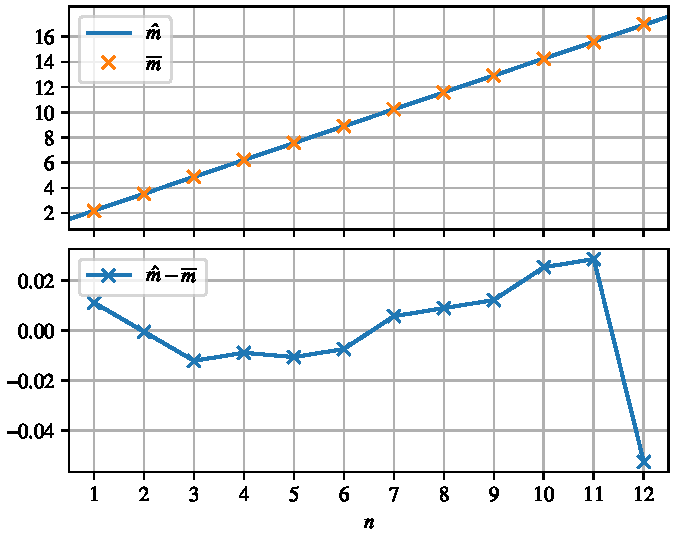
\includegraphics{papers/laguerre/images/estimates.pdf}
%\vspace{-12pt}
\caption{Schätzung Mittelwert von $m$ und Fehler}
\label{laguerre:fig:schaetzung}
\end{figure}

In Abbildung~\ref{laguerre:fig:schaetzung} sind die Resultate
der linearen Regression aufgezeigt mit $\alpha = 1.34094$ und $\beta =
0.854093$.
Die lineare Beziehung ist ganz klar ersichtlich und der Fit scheint zu genügen.
Der optimale Verschiebungsterm kann nun mit
\begin{align*}
m^*
\approx
\lceil \hat{m} - z \rceil
=
\lceil \alpha n + \beta - z \rceil
\end{align*}
% kann nun mit dem linearen Regressor und $z$
gefunden werden.

\subsubsection{Evaluation des Schätzers}
In einem ersten Schritt möchten wir analysieren,
wie gut die Abschätzung des optimalen Verschiebungsterms ist.
Dazu bestimmen wir den relativen Fehler für verschiedene Verschiebungsterme $m$
rund um $m^*$ bei gegebenem Polynomgrad $n = 8$ für $z \in (0, 1)$.
Abbildung~\ref{laguerre:fig:rel_error_shifted} sind die relativen Fehler
der Approximation dargestellt.
Man kann deutlich sehen,
dass der relative Fehler anwächst,
je weiter der Verschiebungsterm vom idealen Wert abweicht.
Zudem scheint der Schätzer den optimalen Verschiebungsterm gut zu bestimmen,
da der Schätzer zuerst der grünen Linie folgt und
dann beim Übergang auf die orange Linie wechselt.
\begin{figure}
\centering
% %% Creator: Matplotlib, PGF backend
%%
%% To include the figure in your LaTeX document, write
%%   \input{<filename>.pgf}
%%
%% Make sure the required packages are loaded in your preamble
%%   \usepackage{pgf}
%%
%% Also ensure that all the required font packages are loaded; for instance,
%% the lmodern package is sometimes necessary when using math font.
%%   \usepackage{lmodern}
%%
%% Figures using additional raster images can only be included by \input if
%% they are in the same directory as the main LaTeX file. For loading figures
%% from other directories you can use the `import` package
%%   \usepackage{import}
%%
%% and then include the figures with
%%   \import{<path to file>}{<filename>.pgf}
%%
%% Matplotlib used the following preamble
%%   \usepackage{fontspec}
%%   \setmainfont{DejaVuSerif.ttf}[Path=\detokenize{/home/mup/.local/lib/python3.8/site-packages/matplotlib/mpl-data/fonts/ttf/}]
%%   \setsansfont{DejaVuSans.ttf}[Path=\detokenize{/home/mup/.local/lib/python3.8/site-packages/matplotlib/mpl-data/fonts/ttf/}]
%%   \setmonofont{DejaVuSansMono.ttf}[Path=\detokenize{/home/mup/.local/lib/python3.8/site-packages/matplotlib/mpl-data/fonts/ttf/}]
%%
\begingroup%
\makeatletter%
\begin{pgfpicture}%
\pgfpathrectangle{\pgfpointorigin}{\pgfqpoint{6.400000in}{4.800000in}}%
\pgfusepath{use as bounding box, clip}%
\begin{pgfscope}%
\pgfsetbuttcap%
\pgfsetmiterjoin%
\definecolor{currentfill}{rgb}{1.000000,1.000000,1.000000}%
\pgfsetfillcolor{currentfill}%
\pgfsetlinewidth{0.000000pt}%
\definecolor{currentstroke}{rgb}{1.000000,1.000000,1.000000}%
\pgfsetstrokecolor{currentstroke}%
\pgfsetdash{}{0pt}%
\pgfpathmoveto{\pgfqpoint{0.000000in}{0.000000in}}%
\pgfpathlineto{\pgfqpoint{6.400000in}{0.000000in}}%
\pgfpathlineto{\pgfqpoint{6.400000in}{4.800000in}}%
\pgfpathlineto{\pgfqpoint{0.000000in}{4.800000in}}%
\pgfpathlineto{\pgfqpoint{0.000000in}{0.000000in}}%
\pgfpathclose%
\pgfusepath{fill}%
\end{pgfscope}%
\begin{pgfscope}%
\pgfsetbuttcap%
\pgfsetmiterjoin%
\definecolor{currentfill}{rgb}{1.000000,1.000000,1.000000}%
\pgfsetfillcolor{currentfill}%
\pgfsetlinewidth{0.000000pt}%
\definecolor{currentstroke}{rgb}{0.000000,0.000000,0.000000}%
\pgfsetstrokecolor{currentstroke}%
\pgfsetstrokeopacity{0.000000}%
\pgfsetdash{}{0pt}%
\pgfpathmoveto{\pgfqpoint{0.426895in}{0.463273in}}%
\pgfpathlineto{\pgfqpoint{6.358330in}{0.463273in}}%
\pgfpathlineto{\pgfqpoint{6.358330in}{4.758330in}}%
\pgfpathlineto{\pgfqpoint{0.426895in}{4.758330in}}%
\pgfpathlineto{\pgfqpoint{0.426895in}{0.463273in}}%
\pgfpathclose%
\pgfusepath{fill}%
\end{pgfscope}%
\begin{pgfscope}%
\pgfpathrectangle{\pgfqpoint{0.426895in}{0.463273in}}{\pgfqpoint{5.931435in}{4.295057in}}%
\pgfusepath{clip}%
\pgfsetrectcap%
\pgfsetroundjoin%
\pgfsetlinewidth{0.803000pt}%
\definecolor{currentstroke}{rgb}{0.690196,0.690196,0.690196}%
\pgfsetstrokecolor{currentstroke}%
\pgfsetdash{}{0pt}%
\pgfpathmoveto{\pgfqpoint{1.595116in}{0.463273in}}%
\pgfpathlineto{\pgfqpoint{1.595116in}{4.758330in}}%
\pgfusepath{stroke}%
\end{pgfscope}%
\begin{pgfscope}%
\pgfsetbuttcap%
\pgfsetroundjoin%
\definecolor{currentfill}{rgb}{0.000000,0.000000,0.000000}%
\pgfsetfillcolor{currentfill}%
\pgfsetlinewidth{0.803000pt}%
\definecolor{currentstroke}{rgb}{0.000000,0.000000,0.000000}%
\pgfsetstrokecolor{currentstroke}%
\pgfsetdash{}{0pt}%
\pgfsys@defobject{currentmarker}{\pgfqpoint{0.000000in}{-0.048611in}}{\pgfqpoint{0.000000in}{0.000000in}}{%
\pgfpathmoveto{\pgfqpoint{0.000000in}{0.000000in}}%
\pgfpathlineto{\pgfqpoint{0.000000in}{-0.048611in}}%
\pgfusepath{stroke,fill}%
}%
\begin{pgfscope}%
\pgfsys@transformshift{1.595116in}{0.463273in}%
\pgfsys@useobject{currentmarker}{}%
\end{pgfscope}%
\end{pgfscope}%
\begin{pgfscope}%
\definecolor{textcolor}{rgb}{0.000000,0.000000,0.000000}%
\pgfsetstrokecolor{textcolor}%
\pgfsetfillcolor{textcolor}%
\pgftext[x=1.595116in,y=0.366051in,,top]{\color{textcolor}\sffamily\fontsize{10.000000}{12.000000}\selectfont 0.2}%
\end{pgfscope}%
\begin{pgfscope}%
\pgfpathrectangle{\pgfqpoint{0.426895in}{0.463273in}}{\pgfqpoint{5.931435in}{4.295057in}}%
\pgfusepath{clip}%
\pgfsetrectcap%
\pgfsetroundjoin%
\pgfsetlinewidth{0.803000pt}%
\definecolor{currentstroke}{rgb}{0.690196,0.690196,0.690196}%
\pgfsetstrokecolor{currentstroke}%
\pgfsetdash{}{0pt}%
\pgfpathmoveto{\pgfqpoint{2.793447in}{0.463273in}}%
\pgfpathlineto{\pgfqpoint{2.793447in}{4.758330in}}%
\pgfusepath{stroke}%
\end{pgfscope}%
\begin{pgfscope}%
\pgfsetbuttcap%
\pgfsetroundjoin%
\definecolor{currentfill}{rgb}{0.000000,0.000000,0.000000}%
\pgfsetfillcolor{currentfill}%
\pgfsetlinewidth{0.803000pt}%
\definecolor{currentstroke}{rgb}{0.000000,0.000000,0.000000}%
\pgfsetstrokecolor{currentstroke}%
\pgfsetdash{}{0pt}%
\pgfsys@defobject{currentmarker}{\pgfqpoint{0.000000in}{-0.048611in}}{\pgfqpoint{0.000000in}{0.000000in}}{%
\pgfpathmoveto{\pgfqpoint{0.000000in}{0.000000in}}%
\pgfpathlineto{\pgfqpoint{0.000000in}{-0.048611in}}%
\pgfusepath{stroke,fill}%
}%
\begin{pgfscope}%
\pgfsys@transformshift{2.793447in}{0.463273in}%
\pgfsys@useobject{currentmarker}{}%
\end{pgfscope}%
\end{pgfscope}%
\begin{pgfscope}%
\definecolor{textcolor}{rgb}{0.000000,0.000000,0.000000}%
\pgfsetstrokecolor{textcolor}%
\pgfsetfillcolor{textcolor}%
\pgftext[x=2.793447in,y=0.366051in,,top]{\color{textcolor}\sffamily\fontsize{10.000000}{12.000000}\selectfont 0.4}%
\end{pgfscope}%
\begin{pgfscope}%
\pgfpathrectangle{\pgfqpoint{0.426895in}{0.463273in}}{\pgfqpoint{5.931435in}{4.295057in}}%
\pgfusepath{clip}%
\pgfsetrectcap%
\pgfsetroundjoin%
\pgfsetlinewidth{0.803000pt}%
\definecolor{currentstroke}{rgb}{0.690196,0.690196,0.690196}%
\pgfsetstrokecolor{currentstroke}%
\pgfsetdash{}{0pt}%
\pgfpathmoveto{\pgfqpoint{3.991778in}{0.463273in}}%
\pgfpathlineto{\pgfqpoint{3.991778in}{4.758330in}}%
\pgfusepath{stroke}%
\end{pgfscope}%
\begin{pgfscope}%
\pgfsetbuttcap%
\pgfsetroundjoin%
\definecolor{currentfill}{rgb}{0.000000,0.000000,0.000000}%
\pgfsetfillcolor{currentfill}%
\pgfsetlinewidth{0.803000pt}%
\definecolor{currentstroke}{rgb}{0.000000,0.000000,0.000000}%
\pgfsetstrokecolor{currentstroke}%
\pgfsetdash{}{0pt}%
\pgfsys@defobject{currentmarker}{\pgfqpoint{0.000000in}{-0.048611in}}{\pgfqpoint{0.000000in}{0.000000in}}{%
\pgfpathmoveto{\pgfqpoint{0.000000in}{0.000000in}}%
\pgfpathlineto{\pgfqpoint{0.000000in}{-0.048611in}}%
\pgfusepath{stroke,fill}%
}%
\begin{pgfscope}%
\pgfsys@transformshift{3.991778in}{0.463273in}%
\pgfsys@useobject{currentmarker}{}%
\end{pgfscope}%
\end{pgfscope}%
\begin{pgfscope}%
\definecolor{textcolor}{rgb}{0.000000,0.000000,0.000000}%
\pgfsetstrokecolor{textcolor}%
\pgfsetfillcolor{textcolor}%
\pgftext[x=3.991778in,y=0.366051in,,top]{\color{textcolor}\sffamily\fontsize{10.000000}{12.000000}\selectfont 0.6}%
\end{pgfscope}%
\begin{pgfscope}%
\pgfpathrectangle{\pgfqpoint{0.426895in}{0.463273in}}{\pgfqpoint{5.931435in}{4.295057in}}%
\pgfusepath{clip}%
\pgfsetrectcap%
\pgfsetroundjoin%
\pgfsetlinewidth{0.803000pt}%
\definecolor{currentstroke}{rgb}{0.690196,0.690196,0.690196}%
\pgfsetstrokecolor{currentstroke}%
\pgfsetdash{}{0pt}%
\pgfpathmoveto{\pgfqpoint{5.190108in}{0.463273in}}%
\pgfpathlineto{\pgfqpoint{5.190108in}{4.758330in}}%
\pgfusepath{stroke}%
\end{pgfscope}%
\begin{pgfscope}%
\pgfsetbuttcap%
\pgfsetroundjoin%
\definecolor{currentfill}{rgb}{0.000000,0.000000,0.000000}%
\pgfsetfillcolor{currentfill}%
\pgfsetlinewidth{0.803000pt}%
\definecolor{currentstroke}{rgb}{0.000000,0.000000,0.000000}%
\pgfsetstrokecolor{currentstroke}%
\pgfsetdash{}{0pt}%
\pgfsys@defobject{currentmarker}{\pgfqpoint{0.000000in}{-0.048611in}}{\pgfqpoint{0.000000in}{0.000000in}}{%
\pgfpathmoveto{\pgfqpoint{0.000000in}{0.000000in}}%
\pgfpathlineto{\pgfqpoint{0.000000in}{-0.048611in}}%
\pgfusepath{stroke,fill}%
}%
\begin{pgfscope}%
\pgfsys@transformshift{5.190108in}{0.463273in}%
\pgfsys@useobject{currentmarker}{}%
\end{pgfscope}%
\end{pgfscope}%
\begin{pgfscope}%
\definecolor{textcolor}{rgb}{0.000000,0.000000,0.000000}%
\pgfsetstrokecolor{textcolor}%
\pgfsetfillcolor{textcolor}%
\pgftext[x=5.190108in,y=0.366051in,,top]{\color{textcolor}\sffamily\fontsize{10.000000}{12.000000}\selectfont 0.8}%
\end{pgfscope}%
\begin{pgfscope}%
\definecolor{textcolor}{rgb}{0.000000,0.000000,0.000000}%
\pgfsetstrokecolor{textcolor}%
\pgfsetfillcolor{textcolor}%
\pgftext[x=3.392612in,y=0.176083in,,top]{\color{textcolor}\sffamily\fontsize{10.000000}{12.000000}\selectfont \(\displaystyle z\)}%
\end{pgfscope}%
\begin{pgfscope}%
\pgfpathrectangle{\pgfqpoint{0.426895in}{0.463273in}}{\pgfqpoint{5.931435in}{4.295057in}}%
\pgfusepath{clip}%
\pgfsetrectcap%
\pgfsetroundjoin%
\pgfsetlinewidth{0.803000pt}%
\definecolor{currentstroke}{rgb}{0.690196,0.690196,0.690196}%
\pgfsetstrokecolor{currentstroke}%
\pgfsetdash{}{0pt}%
\pgfpathmoveto{\pgfqpoint{0.426895in}{1.756214in}}%
\pgfpathlineto{\pgfqpoint{6.358330in}{1.756214in}}%
\pgfusepath{stroke}%
\end{pgfscope}%
\begin{pgfscope}%
\pgfsetbuttcap%
\pgfsetroundjoin%
\definecolor{currentfill}{rgb}{0.000000,0.000000,0.000000}%
\pgfsetfillcolor{currentfill}%
\pgfsetlinewidth{0.803000pt}%
\definecolor{currentstroke}{rgb}{0.000000,0.000000,0.000000}%
\pgfsetstrokecolor{currentstroke}%
\pgfsetdash{}{0pt}%
\pgfsys@defobject{currentmarker}{\pgfqpoint{-0.048611in}{0.000000in}}{\pgfqpoint{-0.000000in}{0.000000in}}{%
\pgfpathmoveto{\pgfqpoint{-0.000000in}{0.000000in}}%
\pgfpathlineto{\pgfqpoint{-0.048611in}{0.000000in}}%
\pgfusepath{stroke,fill}%
}%
\begin{pgfscope}%
\pgfsys@transformshift{0.426895in}{1.756214in}%
\pgfsys@useobject{currentmarker}{}%
\end{pgfscope}%
\end{pgfscope}%
\begin{pgfscope}%
\definecolor{textcolor}{rgb}{0.000000,0.000000,0.000000}%
\pgfsetstrokecolor{textcolor}%
\pgfsetfillcolor{textcolor}%
\pgftext[x=0.041670in, y=1.703453in, left, base]{\color{textcolor}\sffamily\fontsize{10.000000}{12.000000}\selectfont \(\displaystyle {10^{-8}}\)}%
\end{pgfscope}%
\begin{pgfscope}%
\pgfpathrectangle{\pgfqpoint{0.426895in}{0.463273in}}{\pgfqpoint{5.931435in}{4.295057in}}%
\pgfusepath{clip}%
\pgfsetrectcap%
\pgfsetroundjoin%
\pgfsetlinewidth{0.803000pt}%
\definecolor{currentstroke}{rgb}{0.690196,0.690196,0.690196}%
\pgfsetstrokecolor{currentstroke}%
\pgfsetdash{}{0pt}%
\pgfpathmoveto{\pgfqpoint{0.426895in}{0.463273in}}%
\pgfpathlineto{\pgfqpoint{6.358330in}{0.463273in}}%
\pgfusepath{stroke}%
\end{pgfscope}%
\begin{pgfscope}%
\pgfsetbuttcap%
\pgfsetroundjoin%
\definecolor{currentfill}{rgb}{0.000000,0.000000,0.000000}%
\pgfsetfillcolor{currentfill}%
\pgfsetlinewidth{0.602250pt}%
\definecolor{currentstroke}{rgb}{0.000000,0.000000,0.000000}%
\pgfsetstrokecolor{currentstroke}%
\pgfsetdash{}{0pt}%
\pgfsys@defobject{currentmarker}{\pgfqpoint{-0.027778in}{0.000000in}}{\pgfqpoint{-0.000000in}{0.000000in}}{%
\pgfpathmoveto{\pgfqpoint{-0.000000in}{0.000000in}}%
\pgfpathlineto{\pgfqpoint{-0.027778in}{0.000000in}}%
\pgfusepath{stroke,fill}%
}%
\begin{pgfscope}%
\pgfsys@transformshift{0.426895in}{0.463273in}%
\pgfsys@useobject{currentmarker}{}%
\end{pgfscope}%
\end{pgfscope}%
\begin{pgfscope}%
\pgfpathrectangle{\pgfqpoint{0.426895in}{0.463273in}}{\pgfqpoint{5.931435in}{4.295057in}}%
\pgfusepath{clip}%
\pgfsetrectcap%
\pgfsetroundjoin%
\pgfsetlinewidth{0.803000pt}%
\definecolor{currentstroke}{rgb}{0.690196,0.690196,0.690196}%
\pgfsetstrokecolor{currentstroke}%
\pgfsetdash{}{0pt}%
\pgfpathmoveto{\pgfqpoint{0.426895in}{0.803361in}}%
\pgfpathlineto{\pgfqpoint{6.358330in}{0.803361in}}%
\pgfusepath{stroke}%
\end{pgfscope}%
\begin{pgfscope}%
\pgfsetbuttcap%
\pgfsetroundjoin%
\definecolor{currentfill}{rgb}{0.000000,0.000000,0.000000}%
\pgfsetfillcolor{currentfill}%
\pgfsetlinewidth{0.602250pt}%
\definecolor{currentstroke}{rgb}{0.000000,0.000000,0.000000}%
\pgfsetstrokecolor{currentstroke}%
\pgfsetdash{}{0pt}%
\pgfsys@defobject{currentmarker}{\pgfqpoint{-0.027778in}{0.000000in}}{\pgfqpoint{-0.000000in}{0.000000in}}{%
\pgfpathmoveto{\pgfqpoint{-0.000000in}{0.000000in}}%
\pgfpathlineto{\pgfqpoint{-0.027778in}{0.000000in}}%
\pgfusepath{stroke,fill}%
}%
\begin{pgfscope}%
\pgfsys@transformshift{0.426895in}{0.803361in}%
\pgfsys@useobject{currentmarker}{}%
\end{pgfscope}%
\end{pgfscope}%
\begin{pgfscope}%
\pgfpathrectangle{\pgfqpoint{0.426895in}{0.463273in}}{\pgfqpoint{5.931435in}{4.295057in}}%
\pgfusepath{clip}%
\pgfsetrectcap%
\pgfsetroundjoin%
\pgfsetlinewidth{0.803000pt}%
\definecolor{currentstroke}{rgb}{0.690196,0.690196,0.690196}%
\pgfsetstrokecolor{currentstroke}%
\pgfsetdash{}{0pt}%
\pgfpathmoveto{\pgfqpoint{0.426895in}{1.090902in}}%
\pgfpathlineto{\pgfqpoint{6.358330in}{1.090902in}}%
\pgfusepath{stroke}%
\end{pgfscope}%
\begin{pgfscope}%
\pgfsetbuttcap%
\pgfsetroundjoin%
\definecolor{currentfill}{rgb}{0.000000,0.000000,0.000000}%
\pgfsetfillcolor{currentfill}%
\pgfsetlinewidth{0.602250pt}%
\definecolor{currentstroke}{rgb}{0.000000,0.000000,0.000000}%
\pgfsetstrokecolor{currentstroke}%
\pgfsetdash{}{0pt}%
\pgfsys@defobject{currentmarker}{\pgfqpoint{-0.027778in}{0.000000in}}{\pgfqpoint{-0.000000in}{0.000000in}}{%
\pgfpathmoveto{\pgfqpoint{-0.000000in}{0.000000in}}%
\pgfpathlineto{\pgfqpoint{-0.027778in}{0.000000in}}%
\pgfusepath{stroke,fill}%
}%
\begin{pgfscope}%
\pgfsys@transformshift{0.426895in}{1.090902in}%
\pgfsys@useobject{currentmarker}{}%
\end{pgfscope}%
\end{pgfscope}%
\begin{pgfscope}%
\pgfpathrectangle{\pgfqpoint{0.426895in}{0.463273in}}{\pgfqpoint{5.931435in}{4.295057in}}%
\pgfusepath{clip}%
\pgfsetrectcap%
\pgfsetroundjoin%
\pgfsetlinewidth{0.803000pt}%
\definecolor{currentstroke}{rgb}{0.690196,0.690196,0.690196}%
\pgfsetstrokecolor{currentstroke}%
\pgfsetdash{}{0pt}%
\pgfpathmoveto{\pgfqpoint{0.426895in}{1.339980in}}%
\pgfpathlineto{\pgfqpoint{6.358330in}{1.339980in}}%
\pgfusepath{stroke}%
\end{pgfscope}%
\begin{pgfscope}%
\pgfsetbuttcap%
\pgfsetroundjoin%
\definecolor{currentfill}{rgb}{0.000000,0.000000,0.000000}%
\pgfsetfillcolor{currentfill}%
\pgfsetlinewidth{0.602250pt}%
\definecolor{currentstroke}{rgb}{0.000000,0.000000,0.000000}%
\pgfsetstrokecolor{currentstroke}%
\pgfsetdash{}{0pt}%
\pgfsys@defobject{currentmarker}{\pgfqpoint{-0.027778in}{0.000000in}}{\pgfqpoint{-0.000000in}{0.000000in}}{%
\pgfpathmoveto{\pgfqpoint{-0.000000in}{0.000000in}}%
\pgfpathlineto{\pgfqpoint{-0.027778in}{0.000000in}}%
\pgfusepath{stroke,fill}%
}%
\begin{pgfscope}%
\pgfsys@transformshift{0.426895in}{1.339980in}%
\pgfsys@useobject{currentmarker}{}%
\end{pgfscope}%
\end{pgfscope}%
\begin{pgfscope}%
\pgfpathrectangle{\pgfqpoint{0.426895in}{0.463273in}}{\pgfqpoint{5.931435in}{4.295057in}}%
\pgfusepath{clip}%
\pgfsetrectcap%
\pgfsetroundjoin%
\pgfsetlinewidth{0.803000pt}%
\definecolor{currentstroke}{rgb}{0.690196,0.690196,0.690196}%
\pgfsetstrokecolor{currentstroke}%
\pgfsetdash{}{0pt}%
\pgfpathmoveto{\pgfqpoint{0.426895in}{1.559683in}}%
\pgfpathlineto{\pgfqpoint{6.358330in}{1.559683in}}%
\pgfusepath{stroke}%
\end{pgfscope}%
\begin{pgfscope}%
\pgfsetbuttcap%
\pgfsetroundjoin%
\definecolor{currentfill}{rgb}{0.000000,0.000000,0.000000}%
\pgfsetfillcolor{currentfill}%
\pgfsetlinewidth{0.602250pt}%
\definecolor{currentstroke}{rgb}{0.000000,0.000000,0.000000}%
\pgfsetstrokecolor{currentstroke}%
\pgfsetdash{}{0pt}%
\pgfsys@defobject{currentmarker}{\pgfqpoint{-0.027778in}{0.000000in}}{\pgfqpoint{-0.000000in}{0.000000in}}{%
\pgfpathmoveto{\pgfqpoint{-0.000000in}{0.000000in}}%
\pgfpathlineto{\pgfqpoint{-0.027778in}{0.000000in}}%
\pgfusepath{stroke,fill}%
}%
\begin{pgfscope}%
\pgfsys@transformshift{0.426895in}{1.559683in}%
\pgfsys@useobject{currentmarker}{}%
\end{pgfscope}%
\end{pgfscope}%
\begin{pgfscope}%
\pgfpathrectangle{\pgfqpoint{0.426895in}{0.463273in}}{\pgfqpoint{5.931435in}{4.295057in}}%
\pgfusepath{clip}%
\pgfsetrectcap%
\pgfsetroundjoin%
\pgfsetlinewidth{0.803000pt}%
\definecolor{currentstroke}{rgb}{0.690196,0.690196,0.690196}%
\pgfsetstrokecolor{currentstroke}%
\pgfsetdash{}{0pt}%
\pgfpathmoveto{\pgfqpoint{0.426895in}{3.049155in}}%
\pgfpathlineto{\pgfqpoint{6.358330in}{3.049155in}}%
\pgfusepath{stroke}%
\end{pgfscope}%
\begin{pgfscope}%
\pgfsetbuttcap%
\pgfsetroundjoin%
\definecolor{currentfill}{rgb}{0.000000,0.000000,0.000000}%
\pgfsetfillcolor{currentfill}%
\pgfsetlinewidth{0.602250pt}%
\definecolor{currentstroke}{rgb}{0.000000,0.000000,0.000000}%
\pgfsetstrokecolor{currentstroke}%
\pgfsetdash{}{0pt}%
\pgfsys@defobject{currentmarker}{\pgfqpoint{-0.027778in}{0.000000in}}{\pgfqpoint{-0.000000in}{0.000000in}}{%
\pgfpathmoveto{\pgfqpoint{-0.000000in}{0.000000in}}%
\pgfpathlineto{\pgfqpoint{-0.027778in}{0.000000in}}%
\pgfusepath{stroke,fill}%
}%
\begin{pgfscope}%
\pgfsys@transformshift{0.426895in}{3.049155in}%
\pgfsys@useobject{currentmarker}{}%
\end{pgfscope}%
\end{pgfscope}%
\begin{pgfscope}%
\pgfpathrectangle{\pgfqpoint{0.426895in}{0.463273in}}{\pgfqpoint{5.931435in}{4.295057in}}%
\pgfusepath{clip}%
\pgfsetrectcap%
\pgfsetroundjoin%
\pgfsetlinewidth{0.803000pt}%
\definecolor{currentstroke}{rgb}{0.690196,0.690196,0.690196}%
\pgfsetstrokecolor{currentstroke}%
\pgfsetdash{}{0pt}%
\pgfpathmoveto{\pgfqpoint{0.426895in}{3.805477in}}%
\pgfpathlineto{\pgfqpoint{6.358330in}{3.805477in}}%
\pgfusepath{stroke}%
\end{pgfscope}%
\begin{pgfscope}%
\pgfsetbuttcap%
\pgfsetroundjoin%
\definecolor{currentfill}{rgb}{0.000000,0.000000,0.000000}%
\pgfsetfillcolor{currentfill}%
\pgfsetlinewidth{0.602250pt}%
\definecolor{currentstroke}{rgb}{0.000000,0.000000,0.000000}%
\pgfsetstrokecolor{currentstroke}%
\pgfsetdash{}{0pt}%
\pgfsys@defobject{currentmarker}{\pgfqpoint{-0.027778in}{0.000000in}}{\pgfqpoint{-0.000000in}{0.000000in}}{%
\pgfpathmoveto{\pgfqpoint{-0.000000in}{0.000000in}}%
\pgfpathlineto{\pgfqpoint{-0.027778in}{0.000000in}}%
\pgfusepath{stroke,fill}%
}%
\begin{pgfscope}%
\pgfsys@transformshift{0.426895in}{3.805477in}%
\pgfsys@useobject{currentmarker}{}%
\end{pgfscope}%
\end{pgfscope}%
\begin{pgfscope}%
\pgfpathrectangle{\pgfqpoint{0.426895in}{0.463273in}}{\pgfqpoint{5.931435in}{4.295057in}}%
\pgfusepath{clip}%
\pgfsetrectcap%
\pgfsetroundjoin%
\pgfsetlinewidth{0.803000pt}%
\definecolor{currentstroke}{rgb}{0.690196,0.690196,0.690196}%
\pgfsetstrokecolor{currentstroke}%
\pgfsetdash{}{0pt}%
\pgfpathmoveto{\pgfqpoint{0.426895in}{4.342096in}}%
\pgfpathlineto{\pgfqpoint{6.358330in}{4.342096in}}%
\pgfusepath{stroke}%
\end{pgfscope}%
\begin{pgfscope}%
\pgfsetbuttcap%
\pgfsetroundjoin%
\definecolor{currentfill}{rgb}{0.000000,0.000000,0.000000}%
\pgfsetfillcolor{currentfill}%
\pgfsetlinewidth{0.602250pt}%
\definecolor{currentstroke}{rgb}{0.000000,0.000000,0.000000}%
\pgfsetstrokecolor{currentstroke}%
\pgfsetdash{}{0pt}%
\pgfsys@defobject{currentmarker}{\pgfqpoint{-0.027778in}{0.000000in}}{\pgfqpoint{-0.000000in}{0.000000in}}{%
\pgfpathmoveto{\pgfqpoint{-0.000000in}{0.000000in}}%
\pgfpathlineto{\pgfqpoint{-0.027778in}{0.000000in}}%
\pgfusepath{stroke,fill}%
}%
\begin{pgfscope}%
\pgfsys@transformshift{0.426895in}{4.342096in}%
\pgfsys@useobject{currentmarker}{}%
\end{pgfscope}%
\end{pgfscope}%
\begin{pgfscope}%
\pgfpathrectangle{\pgfqpoint{0.426895in}{0.463273in}}{\pgfqpoint{5.931435in}{4.295057in}}%
\pgfusepath{clip}%
\pgfsetrectcap%
\pgfsetroundjoin%
\pgfsetlinewidth{0.803000pt}%
\definecolor{currentstroke}{rgb}{0.690196,0.690196,0.690196}%
\pgfsetstrokecolor{currentstroke}%
\pgfsetdash{}{0pt}%
\pgfpathmoveto{\pgfqpoint{0.426895in}{4.758330in}}%
\pgfpathlineto{\pgfqpoint{6.358330in}{4.758330in}}%
\pgfusepath{stroke}%
\end{pgfscope}%
\begin{pgfscope}%
\pgfsetbuttcap%
\pgfsetroundjoin%
\definecolor{currentfill}{rgb}{0.000000,0.000000,0.000000}%
\pgfsetfillcolor{currentfill}%
\pgfsetlinewidth{0.602250pt}%
\definecolor{currentstroke}{rgb}{0.000000,0.000000,0.000000}%
\pgfsetstrokecolor{currentstroke}%
\pgfsetdash{}{0pt}%
\pgfsys@defobject{currentmarker}{\pgfqpoint{-0.027778in}{0.000000in}}{\pgfqpoint{-0.000000in}{0.000000in}}{%
\pgfpathmoveto{\pgfqpoint{-0.000000in}{0.000000in}}%
\pgfpathlineto{\pgfqpoint{-0.027778in}{0.000000in}}%
\pgfusepath{stroke,fill}%
}%
\begin{pgfscope}%
\pgfsys@transformshift{0.426895in}{4.758330in}%
\pgfsys@useobject{currentmarker}{}%
\end{pgfscope}%
\end{pgfscope}%
\begin{pgfscope}%
\pgfpathrectangle{\pgfqpoint{0.426895in}{0.463273in}}{\pgfqpoint{5.931435in}{4.295057in}}%
\pgfusepath{clip}%
\pgfsetrectcap%
\pgfsetroundjoin%
\pgfsetlinewidth{3.011250pt}%
\definecolor{currentstroke}{rgb}{0.121569,0.466667,0.705882}%
\pgfsetstrokecolor{currentstroke}%
\pgfsetdash{}{0pt}%
\pgfpathmoveto{\pgfqpoint{0.579662in}{0.453273in}}%
\pgfpathlineto{\pgfqpoint{0.604838in}{0.691883in}}%
\pgfpathlineto{\pgfqpoint{0.634495in}{0.934532in}}%
\pgfpathlineto{\pgfqpoint{0.664152in}{1.147779in}}%
\pgfpathlineto{\pgfqpoint{0.693809in}{1.337791in}}%
\pgfpathlineto{\pgfqpoint{0.723466in}{1.508975in}}%
\pgfpathlineto{\pgfqpoint{0.753124in}{1.664580in}}%
\pgfpathlineto{\pgfqpoint{0.782781in}{1.807081in}}%
\pgfpathlineto{\pgfqpoint{0.812438in}{1.938396in}}%
\pgfpathlineto{\pgfqpoint{0.842095in}{2.060050in}}%
\pgfpathlineto{\pgfqpoint{0.871752in}{2.173272in}}%
\pgfpathlineto{\pgfqpoint{0.901410in}{2.279065in}}%
\pgfpathlineto{\pgfqpoint{0.931067in}{2.378263in}}%
\pgfpathlineto{\pgfqpoint{0.960724in}{2.471563in}}%
\pgfpathlineto{\pgfqpoint{0.990381in}{2.559556in}}%
\pgfpathlineto{\pgfqpoint{1.020038in}{2.642744in}}%
\pgfpathlineto{\pgfqpoint{1.049695in}{2.721561in}}%
\pgfpathlineto{\pgfqpoint{1.079353in}{2.796383in}}%
\pgfpathlineto{\pgfqpoint{1.109010in}{2.867537in}}%
\pgfpathlineto{\pgfqpoint{1.138667in}{2.935310in}}%
\pgfpathlineto{\pgfqpoint{1.168324in}{2.999956in}}%
\pgfpathlineto{\pgfqpoint{1.197981in}{3.061700in}}%
\pgfpathlineto{\pgfqpoint{1.227638in}{3.120741in}}%
\pgfpathlineto{\pgfqpoint{1.286953in}{3.231415in}}%
\pgfpathlineto{\pgfqpoint{1.346267in}{3.333204in}}%
\pgfpathlineto{\pgfqpoint{1.405582in}{3.427112in}}%
\pgfpathlineto{\pgfqpoint{1.464896in}{3.513967in}}%
\pgfpathlineto{\pgfqpoint{1.524210in}{3.594465in}}%
\pgfpathlineto{\pgfqpoint{1.583525in}{3.669192in}}%
\pgfpathlineto{\pgfqpoint{1.642839in}{3.738646in}}%
\pgfpathlineto{\pgfqpoint{1.702153in}{3.803258in}}%
\pgfpathlineto{\pgfqpoint{1.761468in}{3.863396in}}%
\pgfpathlineto{\pgfqpoint{1.820782in}{3.919383in}}%
\pgfpathlineto{\pgfqpoint{1.880096in}{3.971501in}}%
\pgfpathlineto{\pgfqpoint{1.939411in}{4.019997in}}%
\pgfpathlineto{\pgfqpoint{1.998725in}{4.065088in}}%
\pgfpathlineto{\pgfqpoint{2.058039in}{4.106968in}}%
\pgfpathlineto{\pgfqpoint{2.117354in}{4.145809in}}%
\pgfpathlineto{\pgfqpoint{2.176668in}{4.181762in}}%
\pgfpathlineto{\pgfqpoint{2.235982in}{4.214965in}}%
\pgfpathlineto{\pgfqpoint{2.295297in}{4.245540in}}%
\pgfpathlineto{\pgfqpoint{2.354611in}{4.273595in}}%
\pgfpathlineto{\pgfqpoint{2.413926in}{4.299228in}}%
\pgfpathlineto{\pgfqpoint{2.473240in}{4.322529in}}%
\pgfpathlineto{\pgfqpoint{2.532554in}{4.343576in}}%
\pgfpathlineto{\pgfqpoint{2.591869in}{4.362440in}}%
\pgfpathlineto{\pgfqpoint{2.651183in}{4.379185in}}%
\pgfpathlineto{\pgfqpoint{2.710497in}{4.393866in}}%
\pgfpathlineto{\pgfqpoint{2.769812in}{4.406536in}}%
\pgfpathlineto{\pgfqpoint{2.829126in}{4.417240in}}%
\pgfpathlineto{\pgfqpoint{2.888440in}{4.426016in}}%
\pgfpathlineto{\pgfqpoint{2.947755in}{4.432901in}}%
\pgfpathlineto{\pgfqpoint{3.007069in}{4.437925in}}%
\pgfpathlineto{\pgfqpoint{3.066383in}{4.441112in}}%
\pgfpathlineto{\pgfqpoint{3.125698in}{4.442487in}}%
\pgfpathlineto{\pgfqpoint{3.185012in}{4.442066in}}%
\pgfpathlineto{\pgfqpoint{3.244326in}{4.439864in}}%
\pgfpathlineto{\pgfqpoint{3.303641in}{4.435891in}}%
\pgfpathlineto{\pgfqpoint{3.362955in}{4.430156in}}%
\pgfpathlineto{\pgfqpoint{3.422270in}{4.422660in}}%
\pgfpathlineto{\pgfqpoint{3.481584in}{4.413405in}}%
\pgfpathlineto{\pgfqpoint{3.540898in}{4.402386in}}%
\pgfpathlineto{\pgfqpoint{3.600213in}{4.389597in}}%
\pgfpathlineto{\pgfqpoint{3.659527in}{4.375027in}}%
\pgfpathlineto{\pgfqpoint{3.718841in}{4.358661in}}%
\pgfpathlineto{\pgfqpoint{3.778156in}{4.340483in}}%
\pgfpathlineto{\pgfqpoint{3.837470in}{4.320469in}}%
\pgfpathlineto{\pgfqpoint{3.896784in}{4.298594in}}%
\pgfpathlineto{\pgfqpoint{3.956099in}{4.274828in}}%
\pgfpathlineto{\pgfqpoint{4.015413in}{4.249135in}}%
\pgfpathlineto{\pgfqpoint{4.074727in}{4.221476in}}%
\pgfpathlineto{\pgfqpoint{4.134042in}{4.191805in}}%
\pgfpathlineto{\pgfqpoint{4.193356in}{4.160072in}}%
\pgfpathlineto{\pgfqpoint{4.252670in}{4.126221in}}%
\pgfpathlineto{\pgfqpoint{4.311985in}{4.090186in}}%
\pgfpathlineto{\pgfqpoint{4.371299in}{4.051899in}}%
\pgfpathlineto{\pgfqpoint{4.430614in}{4.011278in}}%
\pgfpathlineto{\pgfqpoint{4.489928in}{3.968237in}}%
\pgfpathlineto{\pgfqpoint{4.549242in}{3.922678in}}%
\pgfpathlineto{\pgfqpoint{4.608557in}{3.874491in}}%
\pgfpathlineto{\pgfqpoint{4.667871in}{3.823554in}}%
\pgfpathlineto{\pgfqpoint{4.727185in}{3.769730in}}%
\pgfpathlineto{\pgfqpoint{4.786500in}{3.712868in}}%
\pgfpathlineto{\pgfqpoint{4.845814in}{3.652795in}}%
\pgfpathlineto{\pgfqpoint{4.905128in}{3.589319in}}%
\pgfpathlineto{\pgfqpoint{4.964443in}{3.522221in}}%
\pgfpathlineto{\pgfqpoint{5.023757in}{3.451255in}}%
\pgfpathlineto{\pgfqpoint{5.083071in}{3.376139in}}%
\pgfpathlineto{\pgfqpoint{5.142386in}{3.296551in}}%
\pgfpathlineto{\pgfqpoint{5.201700in}{3.212121in}}%
\pgfpathlineto{\pgfqpoint{5.261014in}{3.122420in}}%
\pgfpathlineto{\pgfqpoint{5.320329in}{3.026948in}}%
\pgfpathlineto{\pgfqpoint{5.379643in}{2.925120in}}%
\pgfpathlineto{\pgfqpoint{5.438958in}{2.816240in}}%
\pgfpathlineto{\pgfqpoint{5.498272in}{2.699481in}}%
\pgfpathlineto{\pgfqpoint{5.557586in}{2.573838in}}%
\pgfpathlineto{\pgfqpoint{5.616901in}{2.438086in}}%
\pgfpathlineto{\pgfqpoint{5.646558in}{2.365956in}}%
\pgfpathlineto{\pgfqpoint{5.676215in}{2.290700in}}%
\pgfpathlineto{\pgfqpoint{5.705872in}{2.212064in}}%
\pgfpathlineto{\pgfqpoint{5.735529in}{2.129759in}}%
\pgfpathlineto{\pgfqpoint{5.765186in}{2.043460in}}%
\pgfpathlineto{\pgfqpoint{5.794844in}{1.952790in}}%
\pgfpathlineto{\pgfqpoint{5.824501in}{1.857317in}}%
\pgfpathlineto{\pgfqpoint{5.854158in}{1.756535in}}%
\pgfpathlineto{\pgfqpoint{5.883815in}{1.649857in}}%
\pgfpathlineto{\pgfqpoint{5.913472in}{1.536583in}}%
\pgfpathlineto{\pgfqpoint{5.943130in}{1.415882in}}%
\pgfpathlineto{\pgfqpoint{5.972787in}{1.286747in}}%
\pgfpathlineto{\pgfqpoint{6.002444in}{1.147953in}}%
\pgfpathlineto{\pgfqpoint{6.032101in}{0.997974in}}%
\pgfpathlineto{\pgfqpoint{6.061758in}{0.834889in}}%
\pgfpathlineto{\pgfqpoint{6.091415in}{0.656228in}}%
\pgfpathlineto{\pgfqpoint{6.121807in}{0.453273in}}%
\pgfpathlineto{\pgfqpoint{6.121807in}{0.453273in}}%
\pgfusepath{stroke}%
\end{pgfscope}%
\begin{pgfscope}%
\pgfpathrectangle{\pgfqpoint{0.426895in}{0.463273in}}{\pgfqpoint{5.931435in}{4.295057in}}%
\pgfusepath{clip}%
\pgfsetrectcap%
\pgfsetroundjoin%
\pgfsetlinewidth{3.011250pt}%
\definecolor{currentstroke}{rgb}{1.000000,0.498039,0.054902}%
\pgfsetstrokecolor{currentstroke}%
\pgfsetdash{}{0pt}%
\pgfpathmoveto{\pgfqpoint{0.670534in}{0.453273in}}%
\pgfpathlineto{\pgfqpoint{0.693809in}{0.604192in}}%
\pgfpathlineto{\pgfqpoint{0.723466in}{0.777657in}}%
\pgfpathlineto{\pgfqpoint{0.753124in}{0.935547in}}%
\pgfpathlineto{\pgfqpoint{0.782781in}{1.080329in}}%
\pgfpathlineto{\pgfqpoint{0.812438in}{1.213928in}}%
\pgfpathlineto{\pgfqpoint{0.842095in}{1.337867in}}%
\pgfpathlineto{\pgfqpoint{0.871752in}{1.453373in}}%
\pgfpathlineto{\pgfqpoint{0.901410in}{1.561452in}}%
\pgfpathlineto{\pgfqpoint{0.931067in}{1.662935in}}%
\pgfpathlineto{\pgfqpoint{0.960724in}{1.758522in}}%
\pgfpathlineto{\pgfqpoint{0.990381in}{1.848800in}}%
\pgfpathlineto{\pgfqpoint{1.020038in}{1.934275in}}%
\pgfpathlineto{\pgfqpoint{1.049695in}{2.015380in}}%
\pgfpathlineto{\pgfqpoint{1.079353in}{2.092490in}}%
\pgfpathlineto{\pgfqpoint{1.109010in}{2.165932in}}%
\pgfpathlineto{\pgfqpoint{1.138667in}{2.235994in}}%
\pgfpathlineto{\pgfqpoint{1.168324in}{2.302930in}}%
\pgfpathlineto{\pgfqpoint{1.197981in}{2.366963in}}%
\pgfpathlineto{\pgfqpoint{1.257296in}{2.487104in}}%
\pgfpathlineto{\pgfqpoint{1.316610in}{2.597781in}}%
\pgfpathlineto{\pgfqpoint{1.375924in}{2.700101in}}%
\pgfpathlineto{\pgfqpoint{1.435239in}{2.794975in}}%
\pgfpathlineto{\pgfqpoint{1.494553in}{2.883162in}}%
\pgfpathlineto{\pgfqpoint{1.553867in}{2.965298in}}%
\pgfpathlineto{\pgfqpoint{1.613182in}{3.041924in}}%
\pgfpathlineto{\pgfqpoint{1.672496in}{3.113503in}}%
\pgfpathlineto{\pgfqpoint{1.731810in}{3.180431in}}%
\pgfpathlineto{\pgfqpoint{1.791125in}{3.243056in}}%
\pgfpathlineto{\pgfqpoint{1.850439in}{3.301677in}}%
\pgfpathlineto{\pgfqpoint{1.909754in}{3.356559in}}%
\pgfpathlineto{\pgfqpoint{1.969068in}{3.407933in}}%
\pgfpathlineto{\pgfqpoint{2.028382in}{3.456004in}}%
\pgfpathlineto{\pgfqpoint{2.087697in}{3.500954in}}%
\pgfpathlineto{\pgfqpoint{2.147011in}{3.542945in}}%
\pgfpathlineto{\pgfqpoint{2.206325in}{3.582122in}}%
\pgfpathlineto{\pgfqpoint{2.265640in}{3.618613in}}%
\pgfpathlineto{\pgfqpoint{2.324954in}{3.652533in}}%
\pgfpathlineto{\pgfqpoint{2.384268in}{3.683987in}}%
\pgfpathlineto{\pgfqpoint{2.443583in}{3.713068in}}%
\pgfpathlineto{\pgfqpoint{2.502897in}{3.739858in}}%
\pgfpathlineto{\pgfqpoint{2.562211in}{3.764433in}}%
\pgfpathlineto{\pgfqpoint{2.621526in}{3.786860in}}%
\pgfpathlineto{\pgfqpoint{2.680840in}{3.807199in}}%
\pgfpathlineto{\pgfqpoint{2.740154in}{3.825504in}}%
\pgfpathlineto{\pgfqpoint{2.799469in}{3.841822in}}%
\pgfpathlineto{\pgfqpoint{2.858783in}{3.856197in}}%
\pgfpathlineto{\pgfqpoint{2.918098in}{3.868666in}}%
\pgfpathlineto{\pgfqpoint{2.977412in}{3.879261in}}%
\pgfpathlineto{\pgfqpoint{3.036726in}{3.888010in}}%
\pgfpathlineto{\pgfqpoint{3.096041in}{3.894938in}}%
\pgfpathlineto{\pgfqpoint{3.155355in}{3.900064in}}%
\pgfpathlineto{\pgfqpoint{3.214669in}{3.903406in}}%
\pgfpathlineto{\pgfqpoint{3.273984in}{3.904974in}}%
\pgfpathlineto{\pgfqpoint{3.333298in}{3.904778in}}%
\pgfpathlineto{\pgfqpoint{3.392612in}{3.902824in}}%
\pgfpathlineto{\pgfqpoint{3.451927in}{3.899113in}}%
\pgfpathlineto{\pgfqpoint{3.511241in}{3.893643in}}%
\pgfpathlineto{\pgfqpoint{3.570555in}{3.886409in}}%
\pgfpathlineto{\pgfqpoint{3.629870in}{3.877403in}}%
\pgfpathlineto{\pgfqpoint{3.689184in}{3.866612in}}%
\pgfpathlineto{\pgfqpoint{3.748498in}{3.854020in}}%
\pgfpathlineto{\pgfqpoint{3.807813in}{3.839607in}}%
\pgfpathlineto{\pgfqpoint{3.867127in}{3.823348in}}%
\pgfpathlineto{\pgfqpoint{3.926442in}{3.805217in}}%
\pgfpathlineto{\pgfqpoint{3.985756in}{3.785179in}}%
\pgfpathlineto{\pgfqpoint{4.045070in}{3.763199in}}%
\pgfpathlineto{\pgfqpoint{4.104385in}{3.739233in}}%
\pgfpathlineto{\pgfqpoint{4.163699in}{3.713234in}}%
\pgfpathlineto{\pgfqpoint{4.223013in}{3.685148in}}%
\pgfpathlineto{\pgfqpoint{4.282328in}{3.654915in}}%
\pgfpathlineto{\pgfqpoint{4.341642in}{3.622467in}}%
\pgfpathlineto{\pgfqpoint{4.400956in}{3.587730in}}%
\pgfpathlineto{\pgfqpoint{4.460271in}{3.550622in}}%
\pgfpathlineto{\pgfqpoint{4.519585in}{3.511047in}}%
\pgfpathlineto{\pgfqpoint{4.578899in}{3.468904in}}%
\pgfpathlineto{\pgfqpoint{4.638214in}{3.424076in}}%
\pgfpathlineto{\pgfqpoint{4.697528in}{3.376435in}}%
\pgfpathlineto{\pgfqpoint{4.756842in}{3.325836in}}%
\pgfpathlineto{\pgfqpoint{4.816157in}{3.272118in}}%
\pgfpathlineto{\pgfqpoint{4.875471in}{3.215100in}}%
\pgfpathlineto{\pgfqpoint{4.934786in}{3.154575in}}%
\pgfpathlineto{\pgfqpoint{4.994100in}{3.090312in}}%
\pgfpathlineto{\pgfqpoint{5.053414in}{3.022047in}}%
\pgfpathlineto{\pgfqpoint{5.112729in}{2.949480in}}%
\pgfpathlineto{\pgfqpoint{5.172043in}{2.872266in}}%
\pgfpathlineto{\pgfqpoint{5.231357in}{2.790006in}}%
\pgfpathlineto{\pgfqpoint{5.290672in}{2.702238in}}%
\pgfpathlineto{\pgfqpoint{5.349986in}{2.608422in}}%
\pgfpathlineto{\pgfqpoint{5.409300in}{2.507920in}}%
\pgfpathlineto{\pgfqpoint{5.468615in}{2.399974in}}%
\pgfpathlineto{\pgfqpoint{5.527929in}{2.283675in}}%
\pgfpathlineto{\pgfqpoint{5.587243in}{2.157914in}}%
\pgfpathlineto{\pgfqpoint{5.616901in}{2.091072in}}%
\pgfpathlineto{\pgfqpoint{5.646558in}{2.021328in}}%
\pgfpathlineto{\pgfqpoint{5.676215in}{1.948457in}}%
\pgfpathlineto{\pgfqpoint{5.705872in}{1.872208in}}%
\pgfpathlineto{\pgfqpoint{5.735529in}{1.792291in}}%
\pgfpathlineto{\pgfqpoint{5.765186in}{1.708381in}}%
\pgfpathlineto{\pgfqpoint{5.794844in}{1.620100in}}%
\pgfpathlineto{\pgfqpoint{5.824501in}{1.527017in}}%
\pgfpathlineto{\pgfqpoint{5.854158in}{1.428627in}}%
\pgfpathlineto{\pgfqpoint{5.883815in}{1.324339in}}%
\pgfpathlineto{\pgfqpoint{5.913472in}{1.213459in}}%
\pgfpathlineto{\pgfqpoint{5.943130in}{1.095152in}}%
\pgfpathlineto{\pgfqpoint{5.972787in}{0.968412in}}%
\pgfpathlineto{\pgfqpoint{6.002444in}{0.832012in}}%
\pgfpathlineto{\pgfqpoint{6.032101in}{0.684429in}}%
\pgfpathlineto{\pgfqpoint{6.061758in}{0.523742in}}%
\pgfpathlineto{\pgfqpoint{6.073615in}{0.453273in}}%
\pgfpathlineto{\pgfqpoint{6.073615in}{0.453273in}}%
\pgfusepath{stroke}%
\end{pgfscope}%
\begin{pgfscope}%
\pgfpathrectangle{\pgfqpoint{0.426895in}{0.463273in}}{\pgfqpoint{5.931435in}{4.295057in}}%
\pgfusepath{clip}%
\pgfsetrectcap%
\pgfsetroundjoin%
\pgfsetlinewidth{3.011250pt}%
\definecolor{currentstroke}{rgb}{0.172549,0.627451,0.172549}%
\pgfsetstrokecolor{currentstroke}%
\pgfsetdash{}{0pt}%
\pgfpathmoveto{\pgfqpoint{0.712295in}{0.453273in}}%
\pgfpathlineto{\pgfqpoint{0.723466in}{0.519526in}}%
\pgfpathlineto{\pgfqpoint{0.753124in}{0.679831in}}%
\pgfpathlineto{\pgfqpoint{0.782781in}{0.827033in}}%
\pgfpathlineto{\pgfqpoint{0.812438in}{0.963051in}}%
\pgfpathlineto{\pgfqpoint{0.842095in}{1.089408in}}%
\pgfpathlineto{\pgfqpoint{0.871752in}{1.207335in}}%
\pgfpathlineto{\pgfqpoint{0.901410in}{1.317834in}}%
\pgfpathlineto{\pgfqpoint{0.931067in}{1.421740in}}%
\pgfpathlineto{\pgfqpoint{0.960724in}{1.519749in}}%
\pgfpathlineto{\pgfqpoint{0.990381in}{1.612452in}}%
\pgfpathlineto{\pgfqpoint{1.020038in}{1.700352in}}%
\pgfpathlineto{\pgfqpoint{1.049695in}{1.783883in}}%
\pgfpathlineto{\pgfqpoint{1.079353in}{1.863419in}}%
\pgfpathlineto{\pgfqpoint{1.109010in}{1.939289in}}%
\pgfpathlineto{\pgfqpoint{1.138667in}{2.011779in}}%
\pgfpathlineto{\pgfqpoint{1.168324in}{2.081145in}}%
\pgfpathlineto{\pgfqpoint{1.227638in}{2.211371in}}%
\pgfpathlineto{\pgfqpoint{1.286953in}{2.331492in}}%
\pgfpathlineto{\pgfqpoint{1.346267in}{2.442735in}}%
\pgfpathlineto{\pgfqpoint{1.405582in}{2.546101in}}%
\pgfpathlineto{\pgfqpoint{1.464896in}{2.642422in}}%
\pgfpathlineto{\pgfqpoint{1.524210in}{2.732390in}}%
\pgfpathlineto{\pgfqpoint{1.583525in}{2.816594in}}%
\pgfpathlineto{\pgfqpoint{1.642839in}{2.895530in}}%
\pgfpathlineto{\pgfqpoint{1.702153in}{2.969630in}}%
\pgfpathlineto{\pgfqpoint{1.761468in}{3.039262in}}%
\pgfpathlineto{\pgfqpoint{1.820782in}{3.104750in}}%
\pgfpathlineto{\pgfqpoint{1.880096in}{3.166374in}}%
\pgfpathlineto{\pgfqpoint{1.939411in}{3.224382in}}%
\pgfpathlineto{\pgfqpoint{1.998725in}{3.278992in}}%
\pgfpathlineto{\pgfqpoint{2.058039in}{3.330397in}}%
\pgfpathlineto{\pgfqpoint{2.117354in}{3.378769in}}%
\pgfpathlineto{\pgfqpoint{2.176668in}{3.424259in}}%
\pgfpathlineto{\pgfqpoint{2.235982in}{3.467005in}}%
\pgfpathlineto{\pgfqpoint{2.295297in}{3.507130in}}%
\pgfpathlineto{\pgfqpoint{2.354611in}{3.544741in}}%
\pgfpathlineto{\pgfqpoint{2.413926in}{3.579937in}}%
\pgfpathlineto{\pgfqpoint{2.473240in}{3.612807in}}%
\pgfpathlineto{\pgfqpoint{2.532554in}{3.643429in}}%
\pgfpathlineto{\pgfqpoint{2.591869in}{3.671875in}}%
\pgfpathlineto{\pgfqpoint{2.651183in}{3.698208in}}%
\pgfpathlineto{\pgfqpoint{2.710497in}{3.722484in}}%
\pgfpathlineto{\pgfqpoint{2.769812in}{3.744756in}}%
\pgfpathlineto{\pgfqpoint{2.829126in}{3.765068in}}%
\pgfpathlineto{\pgfqpoint{2.888440in}{3.783459in}}%
\pgfpathlineto{\pgfqpoint{2.947755in}{3.799965in}}%
\pgfpathlineto{\pgfqpoint{3.007069in}{3.814617in}}%
\pgfpathlineto{\pgfqpoint{3.066383in}{3.827441in}}%
\pgfpathlineto{\pgfqpoint{3.125698in}{3.838457in}}%
\pgfpathlineto{\pgfqpoint{3.185012in}{3.847685in}}%
\pgfpathlineto{\pgfqpoint{3.244326in}{3.855139in}}%
\pgfpathlineto{\pgfqpoint{3.303641in}{3.860830in}}%
\pgfpathlineto{\pgfqpoint{3.362955in}{3.864764in}}%
\pgfpathlineto{\pgfqpoint{3.422270in}{3.866946in}}%
\pgfpathlineto{\pgfqpoint{3.481584in}{3.867374in}}%
\pgfpathlineto{\pgfqpoint{3.540898in}{3.866047in}}%
\pgfpathlineto{\pgfqpoint{3.600213in}{3.862956in}}%
\pgfpathlineto{\pgfqpoint{3.659527in}{3.858092in}}%
\pgfpathlineto{\pgfqpoint{3.718841in}{3.851439in}}%
\pgfpathlineto{\pgfqpoint{3.778156in}{3.842981in}}%
\pgfpathlineto{\pgfqpoint{3.837470in}{3.832695in}}%
\pgfpathlineto{\pgfqpoint{3.896784in}{3.820556in}}%
\pgfpathlineto{\pgfqpoint{3.956099in}{3.806532in}}%
\pgfpathlineto{\pgfqpoint{4.015413in}{3.790589in}}%
\pgfpathlineto{\pgfqpoint{4.074727in}{3.772687in}}%
\pgfpathlineto{\pgfqpoint{4.134042in}{3.752782in}}%
\pgfpathlineto{\pgfqpoint{4.193356in}{3.730821in}}%
\pgfpathlineto{\pgfqpoint{4.252670in}{3.706750in}}%
\pgfpathlineto{\pgfqpoint{4.311985in}{3.680504in}}%
\pgfpathlineto{\pgfqpoint{4.371299in}{3.652012in}}%
\pgfpathlineto{\pgfqpoint{4.430614in}{3.621195in}}%
\pgfpathlineto{\pgfqpoint{4.489928in}{3.587965in}}%
\pgfpathlineto{\pgfqpoint{4.549242in}{3.552226in}}%
\pgfpathlineto{\pgfqpoint{4.608557in}{3.513865in}}%
\pgfpathlineto{\pgfqpoint{4.667871in}{3.472763in}}%
\pgfpathlineto{\pgfqpoint{4.727185in}{3.428783in}}%
\pgfpathlineto{\pgfqpoint{4.786500in}{3.381772in}}%
\pgfpathlineto{\pgfqpoint{4.845814in}{3.331558in}}%
\pgfpathlineto{\pgfqpoint{4.905128in}{3.277950in}}%
\pgfpathlineto{\pgfqpoint{4.964443in}{3.220728in}}%
\pgfpathlineto{\pgfqpoint{5.023757in}{3.159645in}}%
\pgfpathlineto{\pgfqpoint{5.083071in}{3.094421in}}%
\pgfpathlineto{\pgfqpoint{5.142386in}{3.024734in}}%
\pgfpathlineto{\pgfqpoint{5.201700in}{2.950212in}}%
\pgfpathlineto{\pgfqpoint{5.261014in}{2.870428in}}%
\pgfpathlineto{\pgfqpoint{5.320329in}{2.784882in}}%
\pgfpathlineto{\pgfqpoint{5.379643in}{2.692988in}}%
\pgfpathlineto{\pgfqpoint{5.438958in}{2.594052in}}%
\pgfpathlineto{\pgfqpoint{5.498272in}{2.487244in}}%
\pgfpathlineto{\pgfqpoint{5.557586in}{2.371561in}}%
\pgfpathlineto{\pgfqpoint{5.587243in}{2.310019in}}%
\pgfpathlineto{\pgfqpoint{5.616901in}{2.245777in}}%
\pgfpathlineto{\pgfqpoint{5.646558in}{2.178636in}}%
\pgfpathlineto{\pgfqpoint{5.676215in}{2.108369in}}%
\pgfpathlineto{\pgfqpoint{5.705872in}{2.034725in}}%
\pgfpathlineto{\pgfqpoint{5.735529in}{1.957415in}}%
\pgfpathlineto{\pgfqpoint{5.765186in}{1.876111in}}%
\pgfpathlineto{\pgfqpoint{5.794844in}{1.790440in}}%
\pgfpathlineto{\pgfqpoint{5.824501in}{1.699968in}}%
\pgfpathlineto{\pgfqpoint{5.854158in}{1.604189in}}%
\pgfpathlineto{\pgfqpoint{5.883815in}{1.502516in}}%
\pgfpathlineto{\pgfqpoint{5.913472in}{1.394249in}}%
\pgfpathlineto{\pgfqpoint{5.943130in}{1.278558in}}%
\pgfpathlineto{\pgfqpoint{5.972787in}{1.154436in}}%
\pgfpathlineto{\pgfqpoint{6.002444in}{1.020656in}}%
\pgfpathlineto{\pgfqpoint{6.032101in}{0.875695in}}%
\pgfpathlineto{\pgfqpoint{6.061758in}{0.717628in}}%
\pgfpathlineto{\pgfqpoint{6.091415in}{0.543988in}}%
\pgfpathlineto{\pgfqpoint{6.105394in}{0.453273in}}%
\pgfpathlineto{\pgfqpoint{6.105394in}{0.453273in}}%
\pgfusepath{stroke}%
\end{pgfscope}%
\begin{pgfscope}%
\pgfpathrectangle{\pgfqpoint{0.426895in}{0.463273in}}{\pgfqpoint{5.931435in}{4.295057in}}%
\pgfusepath{clip}%
\pgfsetrectcap%
\pgfsetroundjoin%
\pgfsetlinewidth{3.011250pt}%
\definecolor{currentstroke}{rgb}{0.839216,0.152941,0.156863}%
\pgfsetstrokecolor{currentstroke}%
\pgfsetdash{}{0pt}%
\pgfpathmoveto{\pgfqpoint{0.672810in}{0.453273in}}%
\pgfpathlineto{\pgfqpoint{0.693809in}{0.593018in}}%
\pgfpathlineto{\pgfqpoint{0.723466in}{0.771553in}}%
\pgfpathlineto{\pgfqpoint{0.753124in}{0.934516in}}%
\pgfpathlineto{\pgfqpoint{0.782781in}{1.084374in}}%
\pgfpathlineto{\pgfqpoint{0.812438in}{1.223051in}}%
\pgfpathlineto{\pgfqpoint{0.842095in}{1.352070in}}%
\pgfpathlineto{\pgfqpoint{0.871752in}{1.472658in}}%
\pgfpathlineto{\pgfqpoint{0.901410in}{1.585823in}}%
\pgfpathlineto{\pgfqpoint{0.931067in}{1.692394in}}%
\pgfpathlineto{\pgfqpoint{0.960724in}{1.793070in}}%
\pgfpathlineto{\pgfqpoint{0.990381in}{1.888441in}}%
\pgfpathlineto{\pgfqpoint{1.020038in}{1.979011in}}%
\pgfpathlineto{\pgfqpoint{1.049695in}{2.065214in}}%
\pgfpathlineto{\pgfqpoint{1.079353in}{2.147424in}}%
\pgfpathlineto{\pgfqpoint{1.109010in}{2.225969in}}%
\pgfpathlineto{\pgfqpoint{1.138667in}{2.301136in}}%
\pgfpathlineto{\pgfqpoint{1.197981in}{2.442322in}}%
\pgfpathlineto{\pgfqpoint{1.257296in}{2.572691in}}%
\pgfpathlineto{\pgfqpoint{1.316610in}{2.693605in}}%
\pgfpathlineto{\pgfqpoint{1.375924in}{2.806173in}}%
\pgfpathlineto{\pgfqpoint{1.435239in}{2.911306in}}%
\pgfpathlineto{\pgfqpoint{1.494553in}{3.009761in}}%
\pgfpathlineto{\pgfqpoint{1.553867in}{3.102176in}}%
\pgfpathlineto{\pgfqpoint{1.613182in}{3.189092in}}%
\pgfpathlineto{\pgfqpoint{1.672496in}{3.270971in}}%
\pgfpathlineto{\pgfqpoint{1.731810in}{3.348210in}}%
\pgfpathlineto{\pgfqpoint{1.791125in}{3.421156in}}%
\pgfpathlineto{\pgfqpoint{1.850439in}{3.490109in}}%
\pgfpathlineto{\pgfqpoint{1.909754in}{3.555333in}}%
\pgfpathlineto{\pgfqpoint{1.969068in}{3.617060in}}%
\pgfpathlineto{\pgfqpoint{2.028382in}{3.675495in}}%
\pgfpathlineto{\pgfqpoint{2.087697in}{3.730821in}}%
\pgfpathlineto{\pgfqpoint{2.147011in}{3.783198in}}%
\pgfpathlineto{\pgfqpoint{2.206325in}{3.832771in}}%
\pgfpathlineto{\pgfqpoint{2.265640in}{3.879670in}}%
\pgfpathlineto{\pgfqpoint{2.324954in}{3.924010in}}%
\pgfpathlineto{\pgfqpoint{2.384268in}{3.965895in}}%
\pgfpathlineto{\pgfqpoint{2.443583in}{4.005417in}}%
\pgfpathlineto{\pgfqpoint{2.502897in}{4.042660in}}%
\pgfpathlineto{\pgfqpoint{2.562211in}{4.077699in}}%
\pgfpathlineto{\pgfqpoint{2.621526in}{4.110602in}}%
\pgfpathlineto{\pgfqpoint{2.680840in}{4.141428in}}%
\pgfpathlineto{\pgfqpoint{2.740154in}{4.170232in}}%
\pgfpathlineto{\pgfqpoint{2.799469in}{4.197061in}}%
\pgfpathlineto{\pgfqpoint{2.858783in}{4.221958in}}%
\pgfpathlineto{\pgfqpoint{2.918098in}{4.244960in}}%
\pgfpathlineto{\pgfqpoint{2.977412in}{4.266101in}}%
\pgfpathlineto{\pgfqpoint{3.036726in}{4.285408in}}%
\pgfpathlineto{\pgfqpoint{3.096041in}{4.302905in}}%
\pgfpathlineto{\pgfqpoint{3.155355in}{4.318613in}}%
\pgfpathlineto{\pgfqpoint{3.214669in}{4.332548in}}%
\pgfpathlineto{\pgfqpoint{3.273984in}{4.344722in}}%
\pgfpathlineto{\pgfqpoint{3.333298in}{4.355144in}}%
\pgfpathlineto{\pgfqpoint{3.392612in}{4.363820in}}%
\pgfpathlineto{\pgfqpoint{3.451927in}{4.370752in}}%
\pgfpathlineto{\pgfqpoint{3.511241in}{4.375937in}}%
\pgfpathlineto{\pgfqpoint{3.570555in}{4.379370in}}%
\pgfpathlineto{\pgfqpoint{3.629870in}{4.381044in}}%
\pgfpathlineto{\pgfqpoint{3.689184in}{4.380945in}}%
\pgfpathlineto{\pgfqpoint{3.748498in}{4.379058in}}%
\pgfpathlineto{\pgfqpoint{3.807813in}{4.375362in}}%
\pgfpathlineto{\pgfqpoint{3.867127in}{4.369835in}}%
\pgfpathlineto{\pgfqpoint{3.926442in}{4.362447in}}%
\pgfpathlineto{\pgfqpoint{3.985756in}{4.353166in}}%
\pgfpathlineto{\pgfqpoint{4.045070in}{4.341955in}}%
\pgfpathlineto{\pgfqpoint{4.104385in}{4.328772in}}%
\pgfpathlineto{\pgfqpoint{4.163699in}{4.313568in}}%
\pgfpathlineto{\pgfqpoint{4.223013in}{4.296291in}}%
\pgfpathlineto{\pgfqpoint{4.282328in}{4.276880in}}%
\pgfpathlineto{\pgfqpoint{4.341642in}{4.255268in}}%
\pgfpathlineto{\pgfqpoint{4.400956in}{4.231380in}}%
\pgfpathlineto{\pgfqpoint{4.460271in}{4.205134in}}%
\pgfpathlineto{\pgfqpoint{4.519585in}{4.176435in}}%
\pgfpathlineto{\pgfqpoint{4.578899in}{4.145182in}}%
\pgfpathlineto{\pgfqpoint{4.638214in}{4.111257in}}%
\pgfpathlineto{\pgfqpoint{4.697528in}{4.074533in}}%
\pgfpathlineto{\pgfqpoint{4.756842in}{4.034866in}}%
\pgfpathlineto{\pgfqpoint{4.816157in}{3.992093in}}%
\pgfpathlineto{\pgfqpoint{4.875471in}{3.946033in}}%
\pgfpathlineto{\pgfqpoint{4.934786in}{3.896482in}}%
\pgfpathlineto{\pgfqpoint{4.994100in}{3.843206in}}%
\pgfpathlineto{\pgfqpoint{5.053414in}{3.785943in}}%
\pgfpathlineto{\pgfqpoint{5.112729in}{3.724392in}}%
\pgfpathlineto{\pgfqpoint{5.172043in}{3.658208in}}%
\pgfpathlineto{\pgfqpoint{5.231357in}{3.586993in}}%
\pgfpathlineto{\pgfqpoint{5.290672in}{3.510285in}}%
\pgfpathlineto{\pgfqpoint{5.349986in}{3.427542in}}%
\pgfpathlineto{\pgfqpoint{5.409300in}{3.338130in}}%
\pgfpathlineto{\pgfqpoint{5.468615in}{3.241288in}}%
\pgfpathlineto{\pgfqpoint{5.527929in}{3.136107in}}%
\pgfpathlineto{\pgfqpoint{5.557586in}{3.080053in}}%
\pgfpathlineto{\pgfqpoint{5.587243in}{3.021480in}}%
\pgfpathlineto{\pgfqpoint{5.616901in}{2.960210in}}%
\pgfpathlineto{\pgfqpoint{5.646558in}{2.896042in}}%
\pgfpathlineto{\pgfqpoint{5.676215in}{2.828751in}}%
\pgfpathlineto{\pgfqpoint{5.705872in}{2.758086in}}%
\pgfpathlineto{\pgfqpoint{5.735529in}{2.683757in}}%
\pgfpathlineto{\pgfqpoint{5.765186in}{2.605438in}}%
\pgfpathlineto{\pgfqpoint{5.794844in}{2.522752in}}%
\pgfpathlineto{\pgfqpoint{5.824501in}{2.435268in}}%
\pgfpathlineto{\pgfqpoint{5.854158in}{2.342481in}}%
\pgfpathlineto{\pgfqpoint{5.883815in}{2.243800in}}%
\pgfpathlineto{\pgfqpoint{5.913472in}{2.138530in}}%
\pgfpathlineto{\pgfqpoint{5.943130in}{2.025837in}}%
\pgfpathlineto{\pgfqpoint{5.972787in}{1.904716in}}%
\pgfpathlineto{\pgfqpoint{6.002444in}{1.773938in}}%
\pgfpathlineto{\pgfqpoint{6.032101in}{1.631981in}}%
\pgfpathlineto{\pgfqpoint{6.061758in}{1.476924in}}%
\pgfpathlineto{\pgfqpoint{6.091415in}{1.306294in}}%
\pgfpathlineto{\pgfqpoint{6.121073in}{1.116841in}}%
\pgfpathlineto{\pgfqpoint{6.150730in}{0.904158in}}%
\pgfpathlineto{\pgfqpoint{6.180387in}{0.662079in}}%
\pgfpathlineto{\pgfqpoint{6.202463in}{0.453273in}}%
\pgfpathlineto{\pgfqpoint{6.202463in}{0.453273in}}%
\pgfusepath{stroke}%
\end{pgfscope}%
\begin{pgfscope}%
\pgfpathrectangle{\pgfqpoint{0.426895in}{0.463273in}}{\pgfqpoint{5.931435in}{4.295057in}}%
\pgfusepath{clip}%
\pgfsetbuttcap%
\pgfsetroundjoin%
\pgfsetlinewidth{3.011250pt}%
\definecolor{currentstroke}{rgb}{0.750000,0.000000,0.750000}%
\pgfsetstrokecolor{currentstroke}%
\pgfsetdash{{3.000000pt}{4.950000pt}}{0.000000pt}%
\pgfpathmoveto{\pgfqpoint{0.712295in}{0.453273in}}%
\pgfpathlineto{\pgfqpoint{0.723466in}{0.519526in}}%
\pgfpathlineto{\pgfqpoint{0.753124in}{0.679831in}}%
\pgfpathlineto{\pgfqpoint{0.782781in}{0.827033in}}%
\pgfpathlineto{\pgfqpoint{0.812438in}{0.963051in}}%
\pgfpathlineto{\pgfqpoint{0.842095in}{1.089408in}}%
\pgfpathlineto{\pgfqpoint{0.871752in}{1.207335in}}%
\pgfpathlineto{\pgfqpoint{0.901410in}{1.317834in}}%
\pgfpathlineto{\pgfqpoint{0.931067in}{1.421740in}}%
\pgfpathlineto{\pgfqpoint{0.960724in}{1.519749in}}%
\pgfpathlineto{\pgfqpoint{0.990381in}{1.612452in}}%
\pgfpathlineto{\pgfqpoint{1.020038in}{1.700352in}}%
\pgfpathlineto{\pgfqpoint{1.049695in}{1.783883in}}%
\pgfpathlineto{\pgfqpoint{1.079353in}{1.863419in}}%
\pgfpathlineto{\pgfqpoint{1.109010in}{1.939289in}}%
\pgfpathlineto{\pgfqpoint{1.138667in}{2.011779in}}%
\pgfpathlineto{\pgfqpoint{1.168324in}{2.081145in}}%
\pgfpathlineto{\pgfqpoint{1.227638in}{2.211371in}}%
\pgfpathlineto{\pgfqpoint{1.286953in}{2.331492in}}%
\pgfpathlineto{\pgfqpoint{1.346267in}{2.442735in}}%
\pgfpathlineto{\pgfqpoint{1.405582in}{2.546101in}}%
\pgfpathlineto{\pgfqpoint{1.464896in}{2.642422in}}%
\pgfpathlineto{\pgfqpoint{1.524210in}{2.732390in}}%
\pgfpathlineto{\pgfqpoint{1.583525in}{2.816594in}}%
\pgfpathlineto{\pgfqpoint{1.642839in}{2.895530in}}%
\pgfpathlineto{\pgfqpoint{1.702153in}{2.969630in}}%
\pgfpathlineto{\pgfqpoint{1.761468in}{3.039262in}}%
\pgfpathlineto{\pgfqpoint{1.820782in}{3.104750in}}%
\pgfpathlineto{\pgfqpoint{1.880096in}{3.166374in}}%
\pgfpathlineto{\pgfqpoint{1.939411in}{3.224382in}}%
\pgfpathlineto{\pgfqpoint{1.998725in}{3.278992in}}%
\pgfpathlineto{\pgfqpoint{2.058039in}{3.330397in}}%
\pgfpathlineto{\pgfqpoint{2.117354in}{3.378769in}}%
\pgfpathlineto{\pgfqpoint{2.176668in}{3.424259in}}%
\pgfpathlineto{\pgfqpoint{2.235982in}{3.467005in}}%
\pgfpathlineto{\pgfqpoint{2.295297in}{3.507130in}}%
\pgfpathlineto{\pgfqpoint{2.354611in}{3.544741in}}%
\pgfpathlineto{\pgfqpoint{2.413926in}{3.579937in}}%
\pgfpathlineto{\pgfqpoint{2.473240in}{3.612807in}}%
\pgfpathlineto{\pgfqpoint{2.532554in}{3.643429in}}%
\pgfpathlineto{\pgfqpoint{2.591869in}{3.671875in}}%
\pgfpathlineto{\pgfqpoint{2.651183in}{3.698208in}}%
\pgfpathlineto{\pgfqpoint{2.710497in}{3.722484in}}%
\pgfpathlineto{\pgfqpoint{2.769812in}{3.744756in}}%
\pgfpathlineto{\pgfqpoint{2.829126in}{3.765068in}}%
\pgfpathlineto{\pgfqpoint{2.888440in}{3.783459in}}%
\pgfpathlineto{\pgfqpoint{2.947755in}{3.799965in}}%
\pgfpathlineto{\pgfqpoint{3.007069in}{3.814617in}}%
\pgfpathlineto{\pgfqpoint{3.066383in}{3.827441in}}%
\pgfpathlineto{\pgfqpoint{3.125698in}{3.838457in}}%
\pgfpathlineto{\pgfqpoint{3.185012in}{3.847685in}}%
\pgfpathlineto{\pgfqpoint{3.244326in}{3.855139in}}%
\pgfpathlineto{\pgfqpoint{3.303641in}{3.860830in}}%
\pgfpathlineto{\pgfqpoint{3.362955in}{3.864764in}}%
\pgfpathlineto{\pgfqpoint{3.422270in}{3.866946in}}%
\pgfpathlineto{\pgfqpoint{3.481584in}{3.867374in}}%
\pgfpathlineto{\pgfqpoint{3.540898in}{3.866047in}}%
\pgfpathlineto{\pgfqpoint{3.600213in}{3.862956in}}%
\pgfpathlineto{\pgfqpoint{3.659527in}{3.858092in}}%
\pgfpathlineto{\pgfqpoint{3.718841in}{3.851439in}}%
\pgfpathlineto{\pgfqpoint{3.778156in}{3.842981in}}%
\pgfpathlineto{\pgfqpoint{3.837470in}{3.832695in}}%
\pgfpathlineto{\pgfqpoint{3.867127in}{3.826859in}}%
\pgfpathlineto{\pgfqpoint{3.896784in}{3.814518in}}%
\pgfpathlineto{\pgfqpoint{3.956099in}{3.795438in}}%
\pgfpathlineto{\pgfqpoint{4.015413in}{3.774435in}}%
\pgfpathlineto{\pgfqpoint{4.074727in}{3.751467in}}%
\pgfpathlineto{\pgfqpoint{4.134042in}{3.726491in}}%
\pgfpathlineto{\pgfqpoint{4.193356in}{3.699455in}}%
\pgfpathlineto{\pgfqpoint{4.252670in}{3.670304in}}%
\pgfpathlineto{\pgfqpoint{4.311985in}{3.638972in}}%
\pgfpathlineto{\pgfqpoint{4.371299in}{3.605390in}}%
\pgfpathlineto{\pgfqpoint{4.430614in}{3.569478in}}%
\pgfpathlineto{\pgfqpoint{4.489928in}{3.531149in}}%
\pgfpathlineto{\pgfqpoint{4.549242in}{3.490303in}}%
\pgfpathlineto{\pgfqpoint{4.608557in}{3.446833in}}%
\pgfpathlineto{\pgfqpoint{4.667871in}{3.400616in}}%
\pgfpathlineto{\pgfqpoint{4.727185in}{3.351515in}}%
\pgfpathlineto{\pgfqpoint{4.786500in}{3.299378in}}%
\pgfpathlineto{\pgfqpoint{4.845814in}{3.244034in}}%
\pgfpathlineto{\pgfqpoint{4.905128in}{3.185289in}}%
\pgfpathlineto{\pgfqpoint{4.964443in}{3.122926in}}%
\pgfpathlineto{\pgfqpoint{5.023757in}{3.056697in}}%
\pgfpathlineto{\pgfqpoint{5.083071in}{2.986322in}}%
\pgfpathlineto{\pgfqpoint{5.142386in}{2.911478in}}%
\pgfpathlineto{\pgfqpoint{5.201700in}{2.831794in}}%
\pgfpathlineto{\pgfqpoint{5.261014in}{2.746842in}}%
\pgfpathlineto{\pgfqpoint{5.320329in}{2.656123in}}%
\pgfpathlineto{\pgfqpoint{5.379643in}{2.559051in}}%
\pgfpathlineto{\pgfqpoint{5.438958in}{2.454931in}}%
\pgfpathlineto{\pgfqpoint{5.498272in}{2.342933in}}%
\pgfpathlineto{\pgfqpoint{5.557586in}{2.222056in}}%
\pgfpathlineto{\pgfqpoint{5.587243in}{2.157914in}}%
\pgfpathlineto{\pgfqpoint{5.616901in}{2.091072in}}%
\pgfpathlineto{\pgfqpoint{5.646558in}{2.021328in}}%
\pgfpathlineto{\pgfqpoint{5.676215in}{1.948457in}}%
\pgfpathlineto{\pgfqpoint{5.705872in}{1.872208in}}%
\pgfpathlineto{\pgfqpoint{5.735529in}{1.792291in}}%
\pgfpathlineto{\pgfqpoint{5.765186in}{1.708381in}}%
\pgfpathlineto{\pgfqpoint{5.794844in}{1.620100in}}%
\pgfpathlineto{\pgfqpoint{5.824501in}{1.527017in}}%
\pgfpathlineto{\pgfqpoint{5.854158in}{1.428627in}}%
\pgfpathlineto{\pgfqpoint{5.883815in}{1.324339in}}%
\pgfpathlineto{\pgfqpoint{5.913472in}{1.213459in}}%
\pgfpathlineto{\pgfqpoint{5.943130in}{1.095152in}}%
\pgfpathlineto{\pgfqpoint{5.972787in}{0.968412in}}%
\pgfpathlineto{\pgfqpoint{6.002444in}{0.832012in}}%
\pgfpathlineto{\pgfqpoint{6.032101in}{0.684429in}}%
\pgfpathlineto{\pgfqpoint{6.061758in}{0.523742in}}%
\pgfpathlineto{\pgfqpoint{6.073615in}{0.453273in}}%
\pgfpathlineto{\pgfqpoint{6.073615in}{0.453273in}}%
\pgfusepath{stroke}%
\end{pgfscope}%
\begin{pgfscope}%
\pgfsetrectcap%
\pgfsetmiterjoin%
\pgfsetlinewidth{0.803000pt}%
\definecolor{currentstroke}{rgb}{0.000000,0.000000,0.000000}%
\pgfsetstrokecolor{currentstroke}%
\pgfsetdash{}{0pt}%
\pgfpathmoveto{\pgfqpoint{0.426895in}{0.463273in}}%
\pgfpathlineto{\pgfqpoint{0.426895in}{4.758330in}}%
\pgfusepath{stroke}%
\end{pgfscope}%
\begin{pgfscope}%
\pgfsetrectcap%
\pgfsetmiterjoin%
\pgfsetlinewidth{0.803000pt}%
\definecolor{currentstroke}{rgb}{0.000000,0.000000,0.000000}%
\pgfsetstrokecolor{currentstroke}%
\pgfsetdash{}{0pt}%
\pgfpathmoveto{\pgfqpoint{6.358330in}{0.463273in}}%
\pgfpathlineto{\pgfqpoint{6.358330in}{4.758330in}}%
\pgfusepath{stroke}%
\end{pgfscope}%
\begin{pgfscope}%
\pgfsetrectcap%
\pgfsetmiterjoin%
\pgfsetlinewidth{0.803000pt}%
\definecolor{currentstroke}{rgb}{0.000000,0.000000,0.000000}%
\pgfsetstrokecolor{currentstroke}%
\pgfsetdash{}{0pt}%
\pgfpathmoveto{\pgfqpoint{0.426895in}{0.463273in}}%
\pgfpathlineto{\pgfqpoint{6.358330in}{0.463273in}}%
\pgfusepath{stroke}%
\end{pgfscope}%
\begin{pgfscope}%
\pgfsetrectcap%
\pgfsetmiterjoin%
\pgfsetlinewidth{0.803000pt}%
\definecolor{currentstroke}{rgb}{0.000000,0.000000,0.000000}%
\pgfsetstrokecolor{currentstroke}%
\pgfsetdash{}{0pt}%
\pgfpathmoveto{\pgfqpoint{0.426895in}{4.758330in}}%
\pgfpathlineto{\pgfqpoint{6.358330in}{4.758330in}}%
\pgfusepath{stroke}%
\end{pgfscope}%
\begin{pgfscope}%
\pgfsetbuttcap%
\pgfsetmiterjoin%
\definecolor{currentfill}{rgb}{1.000000,1.000000,1.000000}%
\pgfsetfillcolor{currentfill}%
\pgfsetfillopacity{0.800000}%
\pgfsetlinewidth{1.003750pt}%
\definecolor{currentstroke}{rgb}{0.800000,0.800000,0.800000}%
\pgfsetstrokecolor{currentstroke}%
\pgfsetstrokeopacity{0.800000}%
\pgfsetdash{}{0pt}%
\pgfpathmoveto{\pgfqpoint{5.370644in}{3.627933in}}%
\pgfpathlineto{\pgfqpoint{6.261108in}{3.627933in}}%
\pgfpathquadraticcurveto{\pgfqpoint{6.288886in}{3.627933in}}{\pgfqpoint{6.288886in}{3.655711in}}%
\pgfpathlineto{\pgfqpoint{6.288886in}{4.661108in}}%
\pgfpathquadraticcurveto{\pgfqpoint{6.288886in}{4.688886in}}{\pgfqpoint{6.261108in}{4.688886in}}%
\pgfpathlineto{\pgfqpoint{5.370644in}{4.688886in}}%
\pgfpathquadraticcurveto{\pgfqpoint{5.342866in}{4.688886in}}{\pgfqpoint{5.342866in}{4.661108in}}%
\pgfpathlineto{\pgfqpoint{5.342866in}{3.655711in}}%
\pgfpathquadraticcurveto{\pgfqpoint{5.342866in}{3.627933in}}{\pgfqpoint{5.370644in}{3.627933in}}%
\pgfpathlineto{\pgfqpoint{5.370644in}{3.627933in}}%
\pgfpathclose%
\pgfusepath{stroke,fill}%
\end{pgfscope}%
\begin{pgfscope}%
\pgfsetrectcap%
\pgfsetroundjoin%
\pgfsetlinewidth{3.011250pt}%
\definecolor{currentstroke}{rgb}{0.121569,0.466667,0.705882}%
\pgfsetstrokecolor{currentstroke}%
\pgfsetdash{}{0pt}%
\pgfpathmoveto{\pgfqpoint{5.398422in}{4.576418in}}%
\pgfpathlineto{\pgfqpoint{5.537311in}{4.576418in}}%
\pgfpathlineto{\pgfqpoint{5.676200in}{4.576418in}}%
\pgfusepath{stroke}%
\end{pgfscope}%
\begin{pgfscope}%
\definecolor{textcolor}{rgb}{0.000000,0.000000,0.000000}%
\pgfsetstrokecolor{textcolor}%
\pgfsetfillcolor{textcolor}%
\pgftext[x=5.787311in,y=4.527807in,left,base]{\color{textcolor}\sffamily\fontsize{10.000000}{12.000000}\selectfont \(\displaystyle m=10\)}%
\end{pgfscope}%
\begin{pgfscope}%
\pgfsetrectcap%
\pgfsetroundjoin%
\pgfsetlinewidth{3.011250pt}%
\definecolor{currentstroke}{rgb}{1.000000,0.498039,0.054902}%
\pgfsetstrokecolor{currentstroke}%
\pgfsetdash{}{0pt}%
\pgfpathmoveto{\pgfqpoint{5.398422in}{4.372561in}}%
\pgfpathlineto{\pgfqpoint{5.537311in}{4.372561in}}%
\pgfpathlineto{\pgfqpoint{5.676200in}{4.372561in}}%
\pgfusepath{stroke}%
\end{pgfscope}%
\begin{pgfscope}%
\definecolor{textcolor}{rgb}{0.000000,0.000000,0.000000}%
\pgfsetstrokecolor{textcolor}%
\pgfsetfillcolor{textcolor}%
\pgftext[x=5.787311in,y=4.323950in,left,base]{\color{textcolor}\sffamily\fontsize{10.000000}{12.000000}\selectfont \(\displaystyle m=11\)}%
\end{pgfscope}%
\begin{pgfscope}%
\pgfsetrectcap%
\pgfsetroundjoin%
\pgfsetlinewidth{3.011250pt}%
\definecolor{currentstroke}{rgb}{0.172549,0.627451,0.172549}%
\pgfsetstrokecolor{currentstroke}%
\pgfsetdash{}{0pt}%
\pgfpathmoveto{\pgfqpoint{5.398422in}{4.168704in}}%
\pgfpathlineto{\pgfqpoint{5.537311in}{4.168704in}}%
\pgfpathlineto{\pgfqpoint{5.676200in}{4.168704in}}%
\pgfusepath{stroke}%
\end{pgfscope}%
\begin{pgfscope}%
\definecolor{textcolor}{rgb}{0.000000,0.000000,0.000000}%
\pgfsetstrokecolor{textcolor}%
\pgfsetfillcolor{textcolor}%
\pgftext[x=5.787311in,y=4.120092in,left,base]{\color{textcolor}\sffamily\fontsize{10.000000}{12.000000}\selectfont \(\displaystyle m=12\)}%
\end{pgfscope}%
\begin{pgfscope}%
\pgfsetrectcap%
\pgfsetroundjoin%
\pgfsetlinewidth{3.011250pt}%
\definecolor{currentstroke}{rgb}{0.839216,0.152941,0.156863}%
\pgfsetstrokecolor{currentstroke}%
\pgfsetdash{}{0pt}%
\pgfpathmoveto{\pgfqpoint{5.398422in}{3.964846in}}%
\pgfpathlineto{\pgfqpoint{5.537311in}{3.964846in}}%
\pgfpathlineto{\pgfqpoint{5.676200in}{3.964846in}}%
\pgfusepath{stroke}%
\end{pgfscope}%
\begin{pgfscope}%
\definecolor{textcolor}{rgb}{0.000000,0.000000,0.000000}%
\pgfsetstrokecolor{textcolor}%
\pgfsetfillcolor{textcolor}%
\pgftext[x=5.787311in,y=3.916235in,left,base]{\color{textcolor}\sffamily\fontsize{10.000000}{12.000000}\selectfont \(\displaystyle m=13\)}%
\end{pgfscope}%
\begin{pgfscope}%
\pgfsetbuttcap%
\pgfsetroundjoin%
\pgfsetlinewidth{3.011250pt}%
\definecolor{currentstroke}{rgb}{0.750000,0.000000,0.750000}%
\pgfsetstrokecolor{currentstroke}%
\pgfsetdash{{3.000000pt}{4.950000pt}}{0.000000pt}%
\pgfpathmoveto{\pgfqpoint{5.398422in}{3.760989in}}%
\pgfpathlineto{\pgfqpoint{5.537311in}{3.760989in}}%
\pgfpathlineto{\pgfqpoint{5.676200in}{3.760989in}}%
\pgfusepath{stroke}%
\end{pgfscope}%
\begin{pgfscope}%
\definecolor{textcolor}{rgb}{0.000000,0.000000,0.000000}%
\pgfsetstrokecolor{textcolor}%
\pgfsetfillcolor{textcolor}%
\pgftext[x=5.787311in,y=3.712378in,left,base]{\color{textcolor}\sffamily\fontsize{10.000000}{12.000000}\selectfont \(\displaystyle m^*\)}%
\end{pgfscope}%
\end{pgfpicture}%
\makeatother%
\endgroup%

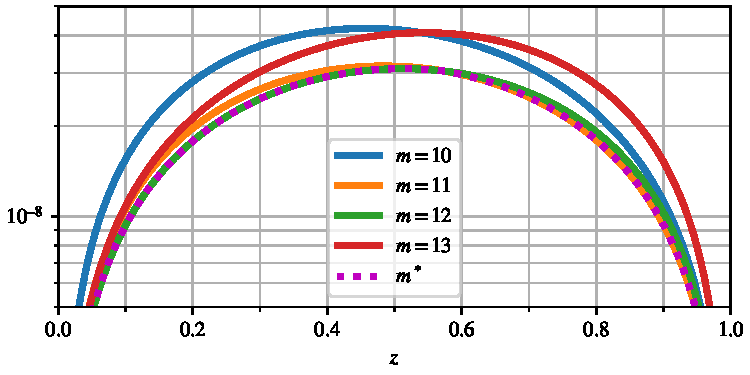
\includegraphics{papers/laguerre/images/rel_error_shifted.pdf}
%\vspace{-12pt}
\caption{Relativer Fehler des Ansatzes mit Verschiebungsterm
für verschiedene reele Werte von $z$ und Verschiebungsterme $m$.
Das verwendete Laguerre-Polynom besitzt den Grad $n = 8$.
$m^*$ bezeichnet hier den optimalen Verschiebungsterm.}
\label{laguerre:fig:rel_error_shifted}
\end{figure}

\subsubsection{Resultate}
Das Verfahren scheint für den Grad $n=8$ und $z \in (0,1)$ gut zu funktioneren.
Es stellt sich nun die Frage,
wie der relative Fehler sich für verschiedene $z$ und $n$ verhält.
In Abbildung~\ref{laguerre:fig:rel_error_range} sind die relativen Fehler für
unterschiedliche $n$ dargestellt.
Der relative Fehler scheint immer noch Nullstellen aufzuweisen
für ganzzahlige $z$.
Durch das Verschieben ergibt sich jetzt aber,
wie zu erwarten war,
ein periodischer relativer Fehler mit einer Periodendauer von $1$.
Zudem lässt sich erkennen,
dass der Fehler abhängig von der Ordnung $n$
des verwendeten Laguerre-Polynoms ist.
Wenn der Grad $n$ um $1$ erhöht wird,
verbessert sich die Genauigkeit des Resultats um etwa eine signifikante Stelle.

In Abbildung~\ref{laguerre:fig:rel_error_complex}
ist der Betrag des relativen Fehlers in der komplexen Ebene dargestellt.
Je stärker der Imaginäranteil von $z$ von $0$ abweicht,
umso schlechter wird die Genauigkeit der Approximation.
Das erstaunt nicht weiter,
da die Gauss-Quadratur eigentlich nur für reelle Zahlen definiert ist.
Wenn der Imaginäranteil von $z$ ungefähr $0$ ist,
lässt sich das gleiche Bild beobachten wie in
Abbildung~\ref{laguerre:fig:rel_error_range}.

\begin{figure}
\centering
% %% Creator: Matplotlib, PGF backend
%%
%% To include the figure in your LaTeX document, write
%%   \input{<filename>.pgf}
%%
%% Make sure the required packages are loaded in your preamble
%%   \usepackage{pgf}
%%
%% Also ensure that all the required font packages are loaded; for instance,
%% the lmodern package is sometimes necessary when using math font.
%%   \usepackage{lmodern}
%%
%% Figures using additional raster images can only be included by \input if
%% they are in the same directory as the main LaTeX file. For loading figures
%% from other directories you can use the `import` package
%%   \usepackage{import}
%%
%% and then include the figures with
%%   \import{<path to file>}{<filename>.pgf}
%%
%% Matplotlib used the following preamble
%%   \usepackage{fontspec}
%%   \setmainfont{DejaVuSerif.ttf}[Path=\detokenize{/home/mup/.local/lib/python3.8/site-packages/matplotlib/mpl-data/fonts/ttf/}]
%%   \setsansfont{DejaVuSans.ttf}[Path=\detokenize{/home/mup/.local/lib/python3.8/site-packages/matplotlib/mpl-data/fonts/ttf/}]
%%   \setmonofont{DejaVuSansMono.ttf}[Path=\detokenize{/home/mup/.local/lib/python3.8/site-packages/matplotlib/mpl-data/fonts/ttf/}]
%%
\begingroup%
\makeatletter%
\begin{pgfpicture}%
\pgfpathrectangle{\pgfpointorigin}{\pgfqpoint{5.000000in}{2.500000in}}%
\pgfusepath{use as bounding box, clip}%
\begin{pgfscope}%
\pgfsetbuttcap%
\pgfsetmiterjoin%
\definecolor{currentfill}{rgb}{1.000000,1.000000,1.000000}%
\pgfsetfillcolor{currentfill}%
\pgfsetlinewidth{0.000000pt}%
\definecolor{currentstroke}{rgb}{1.000000,1.000000,1.000000}%
\pgfsetstrokecolor{currentstroke}%
\pgfsetdash{}{0pt}%
\pgfpathmoveto{\pgfqpoint{0.000000in}{0.000000in}}%
\pgfpathlineto{\pgfqpoint{5.000000in}{0.000000in}}%
\pgfpathlineto{\pgfqpoint{5.000000in}{2.500000in}}%
\pgfpathlineto{\pgfqpoint{0.000000in}{2.500000in}}%
\pgfpathlineto{\pgfqpoint{0.000000in}{0.000000in}}%
\pgfpathclose%
\pgfusepath{fill}%
\end{pgfscope}%
\begin{pgfscope}%
\pgfsetbuttcap%
\pgfsetmiterjoin%
\definecolor{currentfill}{rgb}{1.000000,1.000000,1.000000}%
\pgfsetfillcolor{currentfill}%
\pgfsetlinewidth{0.000000pt}%
\definecolor{currentstroke}{rgb}{0.000000,0.000000,0.000000}%
\pgfsetstrokecolor{currentstroke}%
\pgfsetstrokeopacity{0.000000}%
\pgfsetdash{}{0pt}%
\pgfpathmoveto{\pgfqpoint{0.482257in}{0.463273in}}%
\pgfpathlineto{\pgfqpoint{4.958330in}{0.463273in}}%
\pgfpathlineto{\pgfqpoint{4.958330in}{2.458330in}}%
\pgfpathlineto{\pgfqpoint{0.482257in}{2.458330in}}%
\pgfpathlineto{\pgfqpoint{0.482257in}{0.463273in}}%
\pgfpathclose%
\pgfusepath{fill}%
\end{pgfscope}%
\begin{pgfscope}%
\pgfpathrectangle{\pgfqpoint{0.482257in}{0.463273in}}{\pgfqpoint{4.476072in}{1.995057in}}%
\pgfusepath{clip}%
\pgfsetrectcap%
\pgfsetroundjoin%
\pgfsetlinewidth{0.803000pt}%
\definecolor{currentstroke}{rgb}{0.690196,0.690196,0.690196}%
\pgfsetstrokecolor{currentstroke}%
\pgfsetdash{}{0pt}%
\pgfpathmoveto{\pgfqpoint{0.929865in}{0.463273in}}%
\pgfpathlineto{\pgfqpoint{0.929865in}{2.458330in}}%
\pgfusepath{stroke}%
\end{pgfscope}%
\begin{pgfscope}%
\pgfsetbuttcap%
\pgfsetroundjoin%
\definecolor{currentfill}{rgb}{0.000000,0.000000,0.000000}%
\pgfsetfillcolor{currentfill}%
\pgfsetlinewidth{0.803000pt}%
\definecolor{currentstroke}{rgb}{0.000000,0.000000,0.000000}%
\pgfsetstrokecolor{currentstroke}%
\pgfsetdash{}{0pt}%
\pgfsys@defobject{currentmarker}{\pgfqpoint{0.000000in}{-0.048611in}}{\pgfqpoint{0.000000in}{0.000000in}}{%
\pgfpathmoveto{\pgfqpoint{0.000000in}{0.000000in}}%
\pgfpathlineto{\pgfqpoint{0.000000in}{-0.048611in}}%
\pgfusepath{stroke,fill}%
}%
\begin{pgfscope}%
\pgfsys@transformshift{0.929865in}{0.463273in}%
\pgfsys@useobject{currentmarker}{}%
\end{pgfscope}%
\end{pgfscope}%
\begin{pgfscope}%
\definecolor{textcolor}{rgb}{0.000000,0.000000,0.000000}%
\pgfsetstrokecolor{textcolor}%
\pgfsetfillcolor{textcolor}%
\pgftext[x=0.929865in,y=0.366051in,,top]{\color{textcolor}\sffamily\fontsize{10.000000}{12.000000}\selectfont \ensuremath{-}4}%
\end{pgfscope}%
\begin{pgfscope}%
\pgfpathrectangle{\pgfqpoint{0.482257in}{0.463273in}}{\pgfqpoint{4.476072in}{1.995057in}}%
\pgfusepath{clip}%
\pgfsetrectcap%
\pgfsetroundjoin%
\pgfsetlinewidth{0.803000pt}%
\definecolor{currentstroke}{rgb}{0.690196,0.690196,0.690196}%
\pgfsetstrokecolor{currentstroke}%
\pgfsetdash{}{0pt}%
\pgfpathmoveto{\pgfqpoint{1.825079in}{0.463273in}}%
\pgfpathlineto{\pgfqpoint{1.825079in}{2.458330in}}%
\pgfusepath{stroke}%
\end{pgfscope}%
\begin{pgfscope}%
\pgfsetbuttcap%
\pgfsetroundjoin%
\definecolor{currentfill}{rgb}{0.000000,0.000000,0.000000}%
\pgfsetfillcolor{currentfill}%
\pgfsetlinewidth{0.803000pt}%
\definecolor{currentstroke}{rgb}{0.000000,0.000000,0.000000}%
\pgfsetstrokecolor{currentstroke}%
\pgfsetdash{}{0pt}%
\pgfsys@defobject{currentmarker}{\pgfqpoint{0.000000in}{-0.048611in}}{\pgfqpoint{0.000000in}{0.000000in}}{%
\pgfpathmoveto{\pgfqpoint{0.000000in}{0.000000in}}%
\pgfpathlineto{\pgfqpoint{0.000000in}{-0.048611in}}%
\pgfusepath{stroke,fill}%
}%
\begin{pgfscope}%
\pgfsys@transformshift{1.825079in}{0.463273in}%
\pgfsys@useobject{currentmarker}{}%
\end{pgfscope}%
\end{pgfscope}%
\begin{pgfscope}%
\definecolor{textcolor}{rgb}{0.000000,0.000000,0.000000}%
\pgfsetstrokecolor{textcolor}%
\pgfsetfillcolor{textcolor}%
\pgftext[x=1.825079in,y=0.366051in,,top]{\color{textcolor}\sffamily\fontsize{10.000000}{12.000000}\selectfont \ensuremath{-}2}%
\end{pgfscope}%
\begin{pgfscope}%
\pgfpathrectangle{\pgfqpoint{0.482257in}{0.463273in}}{\pgfqpoint{4.476072in}{1.995057in}}%
\pgfusepath{clip}%
\pgfsetrectcap%
\pgfsetroundjoin%
\pgfsetlinewidth{0.803000pt}%
\definecolor{currentstroke}{rgb}{0.690196,0.690196,0.690196}%
\pgfsetstrokecolor{currentstroke}%
\pgfsetdash{}{0pt}%
\pgfpathmoveto{\pgfqpoint{2.720294in}{0.463273in}}%
\pgfpathlineto{\pgfqpoint{2.720294in}{2.458330in}}%
\pgfusepath{stroke}%
\end{pgfscope}%
\begin{pgfscope}%
\pgfsetbuttcap%
\pgfsetroundjoin%
\definecolor{currentfill}{rgb}{0.000000,0.000000,0.000000}%
\pgfsetfillcolor{currentfill}%
\pgfsetlinewidth{0.803000pt}%
\definecolor{currentstroke}{rgb}{0.000000,0.000000,0.000000}%
\pgfsetstrokecolor{currentstroke}%
\pgfsetdash{}{0pt}%
\pgfsys@defobject{currentmarker}{\pgfqpoint{0.000000in}{-0.048611in}}{\pgfqpoint{0.000000in}{0.000000in}}{%
\pgfpathmoveto{\pgfqpoint{0.000000in}{0.000000in}}%
\pgfpathlineto{\pgfqpoint{0.000000in}{-0.048611in}}%
\pgfusepath{stroke,fill}%
}%
\begin{pgfscope}%
\pgfsys@transformshift{2.720294in}{0.463273in}%
\pgfsys@useobject{currentmarker}{}%
\end{pgfscope}%
\end{pgfscope}%
\begin{pgfscope}%
\definecolor{textcolor}{rgb}{0.000000,0.000000,0.000000}%
\pgfsetstrokecolor{textcolor}%
\pgfsetfillcolor{textcolor}%
\pgftext[x=2.720294in,y=0.366051in,,top]{\color{textcolor}\sffamily\fontsize{10.000000}{12.000000}\selectfont 0}%
\end{pgfscope}%
\begin{pgfscope}%
\pgfpathrectangle{\pgfqpoint{0.482257in}{0.463273in}}{\pgfqpoint{4.476072in}{1.995057in}}%
\pgfusepath{clip}%
\pgfsetrectcap%
\pgfsetroundjoin%
\pgfsetlinewidth{0.803000pt}%
\definecolor{currentstroke}{rgb}{0.690196,0.690196,0.690196}%
\pgfsetstrokecolor{currentstroke}%
\pgfsetdash{}{0pt}%
\pgfpathmoveto{\pgfqpoint{3.615508in}{0.463273in}}%
\pgfpathlineto{\pgfqpoint{3.615508in}{2.458330in}}%
\pgfusepath{stroke}%
\end{pgfscope}%
\begin{pgfscope}%
\pgfsetbuttcap%
\pgfsetroundjoin%
\definecolor{currentfill}{rgb}{0.000000,0.000000,0.000000}%
\pgfsetfillcolor{currentfill}%
\pgfsetlinewidth{0.803000pt}%
\definecolor{currentstroke}{rgb}{0.000000,0.000000,0.000000}%
\pgfsetstrokecolor{currentstroke}%
\pgfsetdash{}{0pt}%
\pgfsys@defobject{currentmarker}{\pgfqpoint{0.000000in}{-0.048611in}}{\pgfqpoint{0.000000in}{0.000000in}}{%
\pgfpathmoveto{\pgfqpoint{0.000000in}{0.000000in}}%
\pgfpathlineto{\pgfqpoint{0.000000in}{-0.048611in}}%
\pgfusepath{stroke,fill}%
}%
\begin{pgfscope}%
\pgfsys@transformshift{3.615508in}{0.463273in}%
\pgfsys@useobject{currentmarker}{}%
\end{pgfscope}%
\end{pgfscope}%
\begin{pgfscope}%
\definecolor{textcolor}{rgb}{0.000000,0.000000,0.000000}%
\pgfsetstrokecolor{textcolor}%
\pgfsetfillcolor{textcolor}%
\pgftext[x=3.615508in,y=0.366051in,,top]{\color{textcolor}\sffamily\fontsize{10.000000}{12.000000}\selectfont 2}%
\end{pgfscope}%
\begin{pgfscope}%
\pgfpathrectangle{\pgfqpoint{0.482257in}{0.463273in}}{\pgfqpoint{4.476072in}{1.995057in}}%
\pgfusepath{clip}%
\pgfsetrectcap%
\pgfsetroundjoin%
\pgfsetlinewidth{0.803000pt}%
\definecolor{currentstroke}{rgb}{0.690196,0.690196,0.690196}%
\pgfsetstrokecolor{currentstroke}%
\pgfsetdash{}{0pt}%
\pgfpathmoveto{\pgfqpoint{4.510723in}{0.463273in}}%
\pgfpathlineto{\pgfqpoint{4.510723in}{2.458330in}}%
\pgfusepath{stroke}%
\end{pgfscope}%
\begin{pgfscope}%
\pgfsetbuttcap%
\pgfsetroundjoin%
\definecolor{currentfill}{rgb}{0.000000,0.000000,0.000000}%
\pgfsetfillcolor{currentfill}%
\pgfsetlinewidth{0.803000pt}%
\definecolor{currentstroke}{rgb}{0.000000,0.000000,0.000000}%
\pgfsetstrokecolor{currentstroke}%
\pgfsetdash{}{0pt}%
\pgfsys@defobject{currentmarker}{\pgfqpoint{0.000000in}{-0.048611in}}{\pgfqpoint{0.000000in}{0.000000in}}{%
\pgfpathmoveto{\pgfqpoint{0.000000in}{0.000000in}}%
\pgfpathlineto{\pgfqpoint{0.000000in}{-0.048611in}}%
\pgfusepath{stroke,fill}%
}%
\begin{pgfscope}%
\pgfsys@transformshift{4.510723in}{0.463273in}%
\pgfsys@useobject{currentmarker}{}%
\end{pgfscope}%
\end{pgfscope}%
\begin{pgfscope}%
\definecolor{textcolor}{rgb}{0.000000,0.000000,0.000000}%
\pgfsetstrokecolor{textcolor}%
\pgfsetfillcolor{textcolor}%
\pgftext[x=4.510723in,y=0.366051in,,top]{\color{textcolor}\sffamily\fontsize{10.000000}{12.000000}\selectfont 4}%
\end{pgfscope}%
\begin{pgfscope}%
\pgfpathrectangle{\pgfqpoint{0.482257in}{0.463273in}}{\pgfqpoint{4.476072in}{1.995057in}}%
\pgfusepath{clip}%
\pgfsetrectcap%
\pgfsetroundjoin%
\pgfsetlinewidth{0.803000pt}%
\definecolor{currentstroke}{rgb}{0.690196,0.690196,0.690196}%
\pgfsetstrokecolor{currentstroke}%
\pgfsetdash{}{0pt}%
\pgfpathmoveto{\pgfqpoint{0.482257in}{0.463273in}}%
\pgfpathlineto{\pgfqpoint{0.482257in}{2.458330in}}%
\pgfusepath{stroke}%
\end{pgfscope}%
\begin{pgfscope}%
\pgfsetbuttcap%
\pgfsetroundjoin%
\definecolor{currentfill}{rgb}{0.000000,0.000000,0.000000}%
\pgfsetfillcolor{currentfill}%
\pgfsetlinewidth{0.602250pt}%
\definecolor{currentstroke}{rgb}{0.000000,0.000000,0.000000}%
\pgfsetstrokecolor{currentstroke}%
\pgfsetdash{}{0pt}%
\pgfsys@defobject{currentmarker}{\pgfqpoint{0.000000in}{-0.027778in}}{\pgfqpoint{0.000000in}{0.000000in}}{%
\pgfpathmoveto{\pgfqpoint{0.000000in}{0.000000in}}%
\pgfpathlineto{\pgfqpoint{0.000000in}{-0.027778in}}%
\pgfusepath{stroke,fill}%
}%
\begin{pgfscope}%
\pgfsys@transformshift{0.482257in}{0.463273in}%
\pgfsys@useobject{currentmarker}{}%
\end{pgfscope}%
\end{pgfscope}%
\begin{pgfscope}%
\pgfpathrectangle{\pgfqpoint{0.482257in}{0.463273in}}{\pgfqpoint{4.476072in}{1.995057in}}%
\pgfusepath{clip}%
\pgfsetrectcap%
\pgfsetroundjoin%
\pgfsetlinewidth{0.803000pt}%
\definecolor{currentstroke}{rgb}{0.690196,0.690196,0.690196}%
\pgfsetstrokecolor{currentstroke}%
\pgfsetdash{}{0pt}%
\pgfpathmoveto{\pgfqpoint{1.377472in}{0.463273in}}%
\pgfpathlineto{\pgfqpoint{1.377472in}{2.458330in}}%
\pgfusepath{stroke}%
\end{pgfscope}%
\begin{pgfscope}%
\pgfsetbuttcap%
\pgfsetroundjoin%
\definecolor{currentfill}{rgb}{0.000000,0.000000,0.000000}%
\pgfsetfillcolor{currentfill}%
\pgfsetlinewidth{0.602250pt}%
\definecolor{currentstroke}{rgb}{0.000000,0.000000,0.000000}%
\pgfsetstrokecolor{currentstroke}%
\pgfsetdash{}{0pt}%
\pgfsys@defobject{currentmarker}{\pgfqpoint{0.000000in}{-0.027778in}}{\pgfqpoint{0.000000in}{0.000000in}}{%
\pgfpathmoveto{\pgfqpoint{0.000000in}{0.000000in}}%
\pgfpathlineto{\pgfqpoint{0.000000in}{-0.027778in}}%
\pgfusepath{stroke,fill}%
}%
\begin{pgfscope}%
\pgfsys@transformshift{1.377472in}{0.463273in}%
\pgfsys@useobject{currentmarker}{}%
\end{pgfscope}%
\end{pgfscope}%
\begin{pgfscope}%
\pgfpathrectangle{\pgfqpoint{0.482257in}{0.463273in}}{\pgfqpoint{4.476072in}{1.995057in}}%
\pgfusepath{clip}%
\pgfsetrectcap%
\pgfsetroundjoin%
\pgfsetlinewidth{0.803000pt}%
\definecolor{currentstroke}{rgb}{0.690196,0.690196,0.690196}%
\pgfsetstrokecolor{currentstroke}%
\pgfsetdash{}{0pt}%
\pgfpathmoveto{\pgfqpoint{2.272687in}{0.463273in}}%
\pgfpathlineto{\pgfqpoint{2.272687in}{2.458330in}}%
\pgfusepath{stroke}%
\end{pgfscope}%
\begin{pgfscope}%
\pgfsetbuttcap%
\pgfsetroundjoin%
\definecolor{currentfill}{rgb}{0.000000,0.000000,0.000000}%
\pgfsetfillcolor{currentfill}%
\pgfsetlinewidth{0.602250pt}%
\definecolor{currentstroke}{rgb}{0.000000,0.000000,0.000000}%
\pgfsetstrokecolor{currentstroke}%
\pgfsetdash{}{0pt}%
\pgfsys@defobject{currentmarker}{\pgfqpoint{0.000000in}{-0.027778in}}{\pgfqpoint{0.000000in}{0.000000in}}{%
\pgfpathmoveto{\pgfqpoint{0.000000in}{0.000000in}}%
\pgfpathlineto{\pgfqpoint{0.000000in}{-0.027778in}}%
\pgfusepath{stroke,fill}%
}%
\begin{pgfscope}%
\pgfsys@transformshift{2.272687in}{0.463273in}%
\pgfsys@useobject{currentmarker}{}%
\end{pgfscope}%
\end{pgfscope}%
\begin{pgfscope}%
\pgfpathrectangle{\pgfqpoint{0.482257in}{0.463273in}}{\pgfqpoint{4.476072in}{1.995057in}}%
\pgfusepath{clip}%
\pgfsetrectcap%
\pgfsetroundjoin%
\pgfsetlinewidth{0.803000pt}%
\definecolor{currentstroke}{rgb}{0.690196,0.690196,0.690196}%
\pgfsetstrokecolor{currentstroke}%
\pgfsetdash{}{0pt}%
\pgfpathmoveto{\pgfqpoint{3.167901in}{0.463273in}}%
\pgfpathlineto{\pgfqpoint{3.167901in}{2.458330in}}%
\pgfusepath{stroke}%
\end{pgfscope}%
\begin{pgfscope}%
\pgfsetbuttcap%
\pgfsetroundjoin%
\definecolor{currentfill}{rgb}{0.000000,0.000000,0.000000}%
\pgfsetfillcolor{currentfill}%
\pgfsetlinewidth{0.602250pt}%
\definecolor{currentstroke}{rgb}{0.000000,0.000000,0.000000}%
\pgfsetstrokecolor{currentstroke}%
\pgfsetdash{}{0pt}%
\pgfsys@defobject{currentmarker}{\pgfqpoint{0.000000in}{-0.027778in}}{\pgfqpoint{0.000000in}{0.000000in}}{%
\pgfpathmoveto{\pgfqpoint{0.000000in}{0.000000in}}%
\pgfpathlineto{\pgfqpoint{0.000000in}{-0.027778in}}%
\pgfusepath{stroke,fill}%
}%
\begin{pgfscope}%
\pgfsys@transformshift{3.167901in}{0.463273in}%
\pgfsys@useobject{currentmarker}{}%
\end{pgfscope}%
\end{pgfscope}%
\begin{pgfscope}%
\pgfpathrectangle{\pgfqpoint{0.482257in}{0.463273in}}{\pgfqpoint{4.476072in}{1.995057in}}%
\pgfusepath{clip}%
\pgfsetrectcap%
\pgfsetroundjoin%
\pgfsetlinewidth{0.803000pt}%
\definecolor{currentstroke}{rgb}{0.690196,0.690196,0.690196}%
\pgfsetstrokecolor{currentstroke}%
\pgfsetdash{}{0pt}%
\pgfpathmoveto{\pgfqpoint{4.063116in}{0.463273in}}%
\pgfpathlineto{\pgfqpoint{4.063116in}{2.458330in}}%
\pgfusepath{stroke}%
\end{pgfscope}%
\begin{pgfscope}%
\pgfsetbuttcap%
\pgfsetroundjoin%
\definecolor{currentfill}{rgb}{0.000000,0.000000,0.000000}%
\pgfsetfillcolor{currentfill}%
\pgfsetlinewidth{0.602250pt}%
\definecolor{currentstroke}{rgb}{0.000000,0.000000,0.000000}%
\pgfsetstrokecolor{currentstroke}%
\pgfsetdash{}{0pt}%
\pgfsys@defobject{currentmarker}{\pgfqpoint{0.000000in}{-0.027778in}}{\pgfqpoint{0.000000in}{0.000000in}}{%
\pgfpathmoveto{\pgfqpoint{0.000000in}{0.000000in}}%
\pgfpathlineto{\pgfqpoint{0.000000in}{-0.027778in}}%
\pgfusepath{stroke,fill}%
}%
\begin{pgfscope}%
\pgfsys@transformshift{4.063116in}{0.463273in}%
\pgfsys@useobject{currentmarker}{}%
\end{pgfscope}%
\end{pgfscope}%
\begin{pgfscope}%
\definecolor{textcolor}{rgb}{0.000000,0.000000,0.000000}%
\pgfsetstrokecolor{textcolor}%
\pgfsetfillcolor{textcolor}%
\pgftext[x=2.720294in,y=0.176083in,,top]{\color{textcolor}\sffamily\fontsize{10.000000}{12.000000}\selectfont \(\displaystyle z\)}%
\end{pgfscope}%
\begin{pgfscope}%
\pgfpathrectangle{\pgfqpoint{0.482257in}{0.463273in}}{\pgfqpoint{4.476072in}{1.995057in}}%
\pgfusepath{clip}%
\pgfsetrectcap%
\pgfsetroundjoin%
\pgfsetlinewidth{0.803000pt}%
\definecolor{currentstroke}{rgb}{0.690196,0.690196,0.690196}%
\pgfsetstrokecolor{currentstroke}%
\pgfsetdash{}{0pt}%
\pgfpathmoveto{\pgfqpoint{0.482257in}{0.463273in}}%
\pgfpathlineto{\pgfqpoint{4.958330in}{0.463273in}}%
\pgfusepath{stroke}%
\end{pgfscope}%
\begin{pgfscope}%
\pgfsetbuttcap%
\pgfsetroundjoin%
\definecolor{currentfill}{rgb}{0.000000,0.000000,0.000000}%
\pgfsetfillcolor{currentfill}%
\pgfsetlinewidth{0.803000pt}%
\definecolor{currentstroke}{rgb}{0.000000,0.000000,0.000000}%
\pgfsetstrokecolor{currentstroke}%
\pgfsetdash{}{0pt}%
\pgfsys@defobject{currentmarker}{\pgfqpoint{-0.048611in}{0.000000in}}{\pgfqpoint{-0.000000in}{0.000000in}}{%
\pgfpathmoveto{\pgfqpoint{-0.000000in}{0.000000in}}%
\pgfpathlineto{\pgfqpoint{-0.048611in}{0.000000in}}%
\pgfusepath{stroke,fill}%
}%
\begin{pgfscope}%
\pgfsys@transformshift{0.482257in}{0.463273in}%
\pgfsys@useobject{currentmarker}{}%
\end{pgfscope}%
\end{pgfscope}%
\begin{pgfscope}%
\definecolor{textcolor}{rgb}{0.000000,0.000000,0.000000}%
\pgfsetstrokecolor{textcolor}%
\pgfsetfillcolor{textcolor}%
\pgftext[x=0.041670in, y=0.410512in, left, base]{\color{textcolor}\sffamily\fontsize{10.000000}{12.000000}\selectfont \(\displaystyle {10^{-11}}\)}%
\end{pgfscope}%
\begin{pgfscope}%
\pgfpathrectangle{\pgfqpoint{0.482257in}{0.463273in}}{\pgfqpoint{4.476072in}{1.995057in}}%
\pgfusepath{clip}%
\pgfsetrectcap%
\pgfsetroundjoin%
\pgfsetlinewidth{0.803000pt}%
\definecolor{currentstroke}{rgb}{0.690196,0.690196,0.690196}%
\pgfsetstrokecolor{currentstroke}%
\pgfsetdash{}{0pt}%
\pgfpathmoveto{\pgfqpoint{0.482257in}{0.870428in}}%
\pgfpathlineto{\pgfqpoint{4.958330in}{0.870428in}}%
\pgfusepath{stroke}%
\end{pgfscope}%
\begin{pgfscope}%
\pgfsetbuttcap%
\pgfsetroundjoin%
\definecolor{currentfill}{rgb}{0.000000,0.000000,0.000000}%
\pgfsetfillcolor{currentfill}%
\pgfsetlinewidth{0.803000pt}%
\definecolor{currentstroke}{rgb}{0.000000,0.000000,0.000000}%
\pgfsetstrokecolor{currentstroke}%
\pgfsetdash{}{0pt}%
\pgfsys@defobject{currentmarker}{\pgfqpoint{-0.048611in}{0.000000in}}{\pgfqpoint{-0.000000in}{0.000000in}}{%
\pgfpathmoveto{\pgfqpoint{-0.000000in}{0.000000in}}%
\pgfpathlineto{\pgfqpoint{-0.048611in}{0.000000in}}%
\pgfusepath{stroke,fill}%
}%
\begin{pgfscope}%
\pgfsys@transformshift{0.482257in}{0.870428in}%
\pgfsys@useobject{currentmarker}{}%
\end{pgfscope}%
\end{pgfscope}%
\begin{pgfscope}%
\definecolor{textcolor}{rgb}{0.000000,0.000000,0.000000}%
\pgfsetstrokecolor{textcolor}%
\pgfsetfillcolor{textcolor}%
\pgftext[x=0.097033in, y=0.817666in, left, base]{\color{textcolor}\sffamily\fontsize{10.000000}{12.000000}\selectfont \(\displaystyle {10^{-9}}\)}%
\end{pgfscope}%
\begin{pgfscope}%
\pgfpathrectangle{\pgfqpoint{0.482257in}{0.463273in}}{\pgfqpoint{4.476072in}{1.995057in}}%
\pgfusepath{clip}%
\pgfsetrectcap%
\pgfsetroundjoin%
\pgfsetlinewidth{0.803000pt}%
\definecolor{currentstroke}{rgb}{0.690196,0.690196,0.690196}%
\pgfsetstrokecolor{currentstroke}%
\pgfsetdash{}{0pt}%
\pgfpathmoveto{\pgfqpoint{0.482257in}{1.277582in}}%
\pgfpathlineto{\pgfqpoint{4.958330in}{1.277582in}}%
\pgfusepath{stroke}%
\end{pgfscope}%
\begin{pgfscope}%
\pgfsetbuttcap%
\pgfsetroundjoin%
\definecolor{currentfill}{rgb}{0.000000,0.000000,0.000000}%
\pgfsetfillcolor{currentfill}%
\pgfsetlinewidth{0.803000pt}%
\definecolor{currentstroke}{rgb}{0.000000,0.000000,0.000000}%
\pgfsetstrokecolor{currentstroke}%
\pgfsetdash{}{0pt}%
\pgfsys@defobject{currentmarker}{\pgfqpoint{-0.048611in}{0.000000in}}{\pgfqpoint{-0.000000in}{0.000000in}}{%
\pgfpathmoveto{\pgfqpoint{-0.000000in}{0.000000in}}%
\pgfpathlineto{\pgfqpoint{-0.048611in}{0.000000in}}%
\pgfusepath{stroke,fill}%
}%
\begin{pgfscope}%
\pgfsys@transformshift{0.482257in}{1.277582in}%
\pgfsys@useobject{currentmarker}{}%
\end{pgfscope}%
\end{pgfscope}%
\begin{pgfscope}%
\definecolor{textcolor}{rgb}{0.000000,0.000000,0.000000}%
\pgfsetstrokecolor{textcolor}%
\pgfsetfillcolor{textcolor}%
\pgftext[x=0.097033in, y=1.224821in, left, base]{\color{textcolor}\sffamily\fontsize{10.000000}{12.000000}\selectfont \(\displaystyle {10^{-7}}\)}%
\end{pgfscope}%
\begin{pgfscope}%
\pgfpathrectangle{\pgfqpoint{0.482257in}{0.463273in}}{\pgfqpoint{4.476072in}{1.995057in}}%
\pgfusepath{clip}%
\pgfsetrectcap%
\pgfsetroundjoin%
\pgfsetlinewidth{0.803000pt}%
\definecolor{currentstroke}{rgb}{0.690196,0.690196,0.690196}%
\pgfsetstrokecolor{currentstroke}%
\pgfsetdash{}{0pt}%
\pgfpathmoveto{\pgfqpoint{0.482257in}{1.684737in}}%
\pgfpathlineto{\pgfqpoint{4.958330in}{1.684737in}}%
\pgfusepath{stroke}%
\end{pgfscope}%
\begin{pgfscope}%
\pgfsetbuttcap%
\pgfsetroundjoin%
\definecolor{currentfill}{rgb}{0.000000,0.000000,0.000000}%
\pgfsetfillcolor{currentfill}%
\pgfsetlinewidth{0.803000pt}%
\definecolor{currentstroke}{rgb}{0.000000,0.000000,0.000000}%
\pgfsetstrokecolor{currentstroke}%
\pgfsetdash{}{0pt}%
\pgfsys@defobject{currentmarker}{\pgfqpoint{-0.048611in}{0.000000in}}{\pgfqpoint{-0.000000in}{0.000000in}}{%
\pgfpathmoveto{\pgfqpoint{-0.000000in}{0.000000in}}%
\pgfpathlineto{\pgfqpoint{-0.048611in}{0.000000in}}%
\pgfusepath{stroke,fill}%
}%
\begin{pgfscope}%
\pgfsys@transformshift{0.482257in}{1.684737in}%
\pgfsys@useobject{currentmarker}{}%
\end{pgfscope}%
\end{pgfscope}%
\begin{pgfscope}%
\definecolor{textcolor}{rgb}{0.000000,0.000000,0.000000}%
\pgfsetstrokecolor{textcolor}%
\pgfsetfillcolor{textcolor}%
\pgftext[x=0.097033in, y=1.631975in, left, base]{\color{textcolor}\sffamily\fontsize{10.000000}{12.000000}\selectfont \(\displaystyle {10^{-5}}\)}%
\end{pgfscope}%
\begin{pgfscope}%
\pgfpathrectangle{\pgfqpoint{0.482257in}{0.463273in}}{\pgfqpoint{4.476072in}{1.995057in}}%
\pgfusepath{clip}%
\pgfsetrectcap%
\pgfsetroundjoin%
\pgfsetlinewidth{0.803000pt}%
\definecolor{currentstroke}{rgb}{0.690196,0.690196,0.690196}%
\pgfsetstrokecolor{currentstroke}%
\pgfsetdash{}{0pt}%
\pgfpathmoveto{\pgfqpoint{0.482257in}{2.091891in}}%
\pgfpathlineto{\pgfqpoint{4.958330in}{2.091891in}}%
\pgfusepath{stroke}%
\end{pgfscope}%
\begin{pgfscope}%
\pgfsetbuttcap%
\pgfsetroundjoin%
\definecolor{currentfill}{rgb}{0.000000,0.000000,0.000000}%
\pgfsetfillcolor{currentfill}%
\pgfsetlinewidth{0.803000pt}%
\definecolor{currentstroke}{rgb}{0.000000,0.000000,0.000000}%
\pgfsetstrokecolor{currentstroke}%
\pgfsetdash{}{0pt}%
\pgfsys@defobject{currentmarker}{\pgfqpoint{-0.048611in}{0.000000in}}{\pgfqpoint{-0.000000in}{0.000000in}}{%
\pgfpathmoveto{\pgfqpoint{-0.000000in}{0.000000in}}%
\pgfpathlineto{\pgfqpoint{-0.048611in}{0.000000in}}%
\pgfusepath{stroke,fill}%
}%
\begin{pgfscope}%
\pgfsys@transformshift{0.482257in}{2.091891in}%
\pgfsys@useobject{currentmarker}{}%
\end{pgfscope}%
\end{pgfscope}%
\begin{pgfscope}%
\definecolor{textcolor}{rgb}{0.000000,0.000000,0.000000}%
\pgfsetstrokecolor{textcolor}%
\pgfsetfillcolor{textcolor}%
\pgftext[x=0.097033in, y=2.039129in, left, base]{\color{textcolor}\sffamily\fontsize{10.000000}{12.000000}\selectfont \(\displaystyle {10^{-3}}\)}%
\end{pgfscope}%
\begin{pgfscope}%
\pgfpathrectangle{\pgfqpoint{0.482257in}{0.463273in}}{\pgfqpoint{4.476072in}{1.995057in}}%
\pgfusepath{clip}%
\pgfsetrectcap%
\pgfsetroundjoin%
\pgfsetlinewidth{0.803000pt}%
\definecolor{currentstroke}{rgb}{0.690196,0.690196,0.690196}%
\pgfsetstrokecolor{currentstroke}%
\pgfsetdash{}{0pt}%
\pgfpathmoveto{\pgfqpoint{0.482257in}{0.666851in}}%
\pgfpathlineto{\pgfqpoint{4.958330in}{0.666851in}}%
\pgfusepath{stroke}%
\end{pgfscope}%
\begin{pgfscope}%
\pgfsetbuttcap%
\pgfsetroundjoin%
\definecolor{currentfill}{rgb}{0.000000,0.000000,0.000000}%
\pgfsetfillcolor{currentfill}%
\pgfsetlinewidth{0.602250pt}%
\definecolor{currentstroke}{rgb}{0.000000,0.000000,0.000000}%
\pgfsetstrokecolor{currentstroke}%
\pgfsetdash{}{0pt}%
\pgfsys@defobject{currentmarker}{\pgfqpoint{-0.027778in}{0.000000in}}{\pgfqpoint{-0.000000in}{0.000000in}}{%
\pgfpathmoveto{\pgfqpoint{-0.000000in}{0.000000in}}%
\pgfpathlineto{\pgfqpoint{-0.027778in}{0.000000in}}%
\pgfusepath{stroke,fill}%
}%
\begin{pgfscope}%
\pgfsys@transformshift{0.482257in}{0.666851in}%
\pgfsys@useobject{currentmarker}{}%
\end{pgfscope}%
\end{pgfscope}%
\begin{pgfscope}%
\definecolor{textcolor}{rgb}{0.000000,0.000000,0.000000}%
\pgfsetstrokecolor{textcolor}%
\pgfsetfillcolor{textcolor}%
\pgftext[x=0.063892in, y=0.614089in, left, base]{\color{textcolor}\sffamily\fontsize{10.000000}{12.000000}\selectfont \(\displaystyle {10^{-10}}\)}%
\end{pgfscope}%
\begin{pgfscope}%
\pgfpathrectangle{\pgfqpoint{0.482257in}{0.463273in}}{\pgfqpoint{4.476072in}{1.995057in}}%
\pgfusepath{clip}%
\pgfsetrectcap%
\pgfsetroundjoin%
\pgfsetlinewidth{0.803000pt}%
\definecolor{currentstroke}{rgb}{0.690196,0.690196,0.690196}%
\pgfsetstrokecolor{currentstroke}%
\pgfsetdash{}{0pt}%
\pgfpathmoveto{\pgfqpoint{0.482257in}{1.074005in}}%
\pgfpathlineto{\pgfqpoint{4.958330in}{1.074005in}}%
\pgfusepath{stroke}%
\end{pgfscope}%
\begin{pgfscope}%
\pgfsetbuttcap%
\pgfsetroundjoin%
\definecolor{currentfill}{rgb}{0.000000,0.000000,0.000000}%
\pgfsetfillcolor{currentfill}%
\pgfsetlinewidth{0.602250pt}%
\definecolor{currentstroke}{rgb}{0.000000,0.000000,0.000000}%
\pgfsetstrokecolor{currentstroke}%
\pgfsetdash{}{0pt}%
\pgfsys@defobject{currentmarker}{\pgfqpoint{-0.027778in}{0.000000in}}{\pgfqpoint{-0.000000in}{0.000000in}}{%
\pgfpathmoveto{\pgfqpoint{-0.000000in}{0.000000in}}%
\pgfpathlineto{\pgfqpoint{-0.027778in}{0.000000in}}%
\pgfusepath{stroke,fill}%
}%
\begin{pgfscope}%
\pgfsys@transformshift{0.482257in}{1.074005in}%
\pgfsys@useobject{currentmarker}{}%
\end{pgfscope}%
\end{pgfscope}%
\begin{pgfscope}%
\definecolor{textcolor}{rgb}{0.000000,0.000000,0.000000}%
\pgfsetstrokecolor{textcolor}%
\pgfsetfillcolor{textcolor}%
\pgftext[x=0.119255in, y=1.021243in, left, base]{\color{textcolor}\sffamily\fontsize{10.000000}{12.000000}\selectfont \(\displaystyle {10^{-8}}\)}%
\end{pgfscope}%
\begin{pgfscope}%
\pgfpathrectangle{\pgfqpoint{0.482257in}{0.463273in}}{\pgfqpoint{4.476072in}{1.995057in}}%
\pgfusepath{clip}%
\pgfsetrectcap%
\pgfsetroundjoin%
\pgfsetlinewidth{0.803000pt}%
\definecolor{currentstroke}{rgb}{0.690196,0.690196,0.690196}%
\pgfsetstrokecolor{currentstroke}%
\pgfsetdash{}{0pt}%
\pgfpathmoveto{\pgfqpoint{0.482257in}{1.481159in}}%
\pgfpathlineto{\pgfqpoint{4.958330in}{1.481159in}}%
\pgfusepath{stroke}%
\end{pgfscope}%
\begin{pgfscope}%
\pgfsetbuttcap%
\pgfsetroundjoin%
\definecolor{currentfill}{rgb}{0.000000,0.000000,0.000000}%
\pgfsetfillcolor{currentfill}%
\pgfsetlinewidth{0.602250pt}%
\definecolor{currentstroke}{rgb}{0.000000,0.000000,0.000000}%
\pgfsetstrokecolor{currentstroke}%
\pgfsetdash{}{0pt}%
\pgfsys@defobject{currentmarker}{\pgfqpoint{-0.027778in}{0.000000in}}{\pgfqpoint{-0.000000in}{0.000000in}}{%
\pgfpathmoveto{\pgfqpoint{-0.000000in}{0.000000in}}%
\pgfpathlineto{\pgfqpoint{-0.027778in}{0.000000in}}%
\pgfusepath{stroke,fill}%
}%
\begin{pgfscope}%
\pgfsys@transformshift{0.482257in}{1.481159in}%
\pgfsys@useobject{currentmarker}{}%
\end{pgfscope}%
\end{pgfscope}%
\begin{pgfscope}%
\definecolor{textcolor}{rgb}{0.000000,0.000000,0.000000}%
\pgfsetstrokecolor{textcolor}%
\pgfsetfillcolor{textcolor}%
\pgftext[x=0.119255in, y=1.428398in, left, base]{\color{textcolor}\sffamily\fontsize{10.000000}{12.000000}\selectfont \(\displaystyle {10^{-6}}\)}%
\end{pgfscope}%
\begin{pgfscope}%
\pgfpathrectangle{\pgfqpoint{0.482257in}{0.463273in}}{\pgfqpoint{4.476072in}{1.995057in}}%
\pgfusepath{clip}%
\pgfsetrectcap%
\pgfsetroundjoin%
\pgfsetlinewidth{0.803000pt}%
\definecolor{currentstroke}{rgb}{0.690196,0.690196,0.690196}%
\pgfsetstrokecolor{currentstroke}%
\pgfsetdash{}{0pt}%
\pgfpathmoveto{\pgfqpoint{0.482257in}{1.888314in}}%
\pgfpathlineto{\pgfqpoint{4.958330in}{1.888314in}}%
\pgfusepath{stroke}%
\end{pgfscope}%
\begin{pgfscope}%
\pgfsetbuttcap%
\pgfsetroundjoin%
\definecolor{currentfill}{rgb}{0.000000,0.000000,0.000000}%
\pgfsetfillcolor{currentfill}%
\pgfsetlinewidth{0.602250pt}%
\definecolor{currentstroke}{rgb}{0.000000,0.000000,0.000000}%
\pgfsetstrokecolor{currentstroke}%
\pgfsetdash{}{0pt}%
\pgfsys@defobject{currentmarker}{\pgfqpoint{-0.027778in}{0.000000in}}{\pgfqpoint{-0.000000in}{0.000000in}}{%
\pgfpathmoveto{\pgfqpoint{-0.000000in}{0.000000in}}%
\pgfpathlineto{\pgfqpoint{-0.027778in}{0.000000in}}%
\pgfusepath{stroke,fill}%
}%
\begin{pgfscope}%
\pgfsys@transformshift{0.482257in}{1.888314in}%
\pgfsys@useobject{currentmarker}{}%
\end{pgfscope}%
\end{pgfscope}%
\begin{pgfscope}%
\definecolor{textcolor}{rgb}{0.000000,0.000000,0.000000}%
\pgfsetstrokecolor{textcolor}%
\pgfsetfillcolor{textcolor}%
\pgftext[x=0.119255in, y=1.835552in, left, base]{\color{textcolor}\sffamily\fontsize{10.000000}{12.000000}\selectfont \(\displaystyle {10^{-4}}\)}%
\end{pgfscope}%
\begin{pgfscope}%
\pgfpathrectangle{\pgfqpoint{0.482257in}{0.463273in}}{\pgfqpoint{4.476072in}{1.995057in}}%
\pgfusepath{clip}%
\pgfsetrectcap%
\pgfsetroundjoin%
\pgfsetlinewidth{0.803000pt}%
\definecolor{currentstroke}{rgb}{0.690196,0.690196,0.690196}%
\pgfsetstrokecolor{currentstroke}%
\pgfsetdash{}{0pt}%
\pgfpathmoveto{\pgfqpoint{0.482257in}{2.295468in}}%
\pgfpathlineto{\pgfqpoint{4.958330in}{2.295468in}}%
\pgfusepath{stroke}%
\end{pgfscope}%
\begin{pgfscope}%
\pgfsetbuttcap%
\pgfsetroundjoin%
\definecolor{currentfill}{rgb}{0.000000,0.000000,0.000000}%
\pgfsetfillcolor{currentfill}%
\pgfsetlinewidth{0.602250pt}%
\definecolor{currentstroke}{rgb}{0.000000,0.000000,0.000000}%
\pgfsetstrokecolor{currentstroke}%
\pgfsetdash{}{0pt}%
\pgfsys@defobject{currentmarker}{\pgfqpoint{-0.027778in}{0.000000in}}{\pgfqpoint{-0.000000in}{0.000000in}}{%
\pgfpathmoveto{\pgfqpoint{-0.000000in}{0.000000in}}%
\pgfpathlineto{\pgfqpoint{-0.027778in}{0.000000in}}%
\pgfusepath{stroke,fill}%
}%
\begin{pgfscope}%
\pgfsys@transformshift{0.482257in}{2.295468in}%
\pgfsys@useobject{currentmarker}{}%
\end{pgfscope}%
\end{pgfscope}%
\begin{pgfscope}%
\definecolor{textcolor}{rgb}{0.000000,0.000000,0.000000}%
\pgfsetstrokecolor{textcolor}%
\pgfsetfillcolor{textcolor}%
\pgftext[x=0.119255in, y=2.242707in, left, base]{\color{textcolor}\sffamily\fontsize{10.000000}{12.000000}\selectfont \(\displaystyle {10^{-2}}\)}%
\end{pgfscope}%
\begin{pgfscope}%
\pgfpathrectangle{\pgfqpoint{0.482257in}{0.463273in}}{\pgfqpoint{4.476072in}{1.995057in}}%
\pgfusepath{clip}%
\pgfsetrectcap%
\pgfsetroundjoin%
\pgfsetlinewidth{1.505625pt}%
\definecolor{currentstroke}{rgb}{0.121569,0.466667,0.705882}%
\pgfsetstrokecolor{currentstroke}%
\pgfsetdash{}{0pt}%
\pgfpathmoveto{\pgfqpoint{0.482258in}{1.007279in}}%
\pgfpathlineto{\pgfqpoint{0.486738in}{2.025203in}}%
\pgfpathlineto{\pgfqpoint{0.491219in}{2.086414in}}%
\pgfpathlineto{\pgfqpoint{0.495699in}{2.122169in}}%
\pgfpathlineto{\pgfqpoint{0.504660in}{2.167085in}}%
\pgfpathlineto{\pgfqpoint{0.513621in}{2.196503in}}%
\pgfpathlineto{\pgfqpoint{0.522583in}{2.218308in}}%
\pgfpathlineto{\pgfqpoint{0.531544in}{2.235552in}}%
\pgfpathlineto{\pgfqpoint{0.544985in}{2.255967in}}%
\pgfpathlineto{\pgfqpoint{0.558427in}{2.272033in}}%
\pgfpathlineto{\pgfqpoint{0.571869in}{2.285104in}}%
\pgfpathlineto{\pgfqpoint{0.589791in}{2.299176in}}%
\pgfpathlineto{\pgfqpoint{0.607713in}{2.310379in}}%
\pgfpathlineto{\pgfqpoint{0.630116in}{2.321308in}}%
\pgfpathlineto{\pgfqpoint{0.652519in}{2.329506in}}%
\pgfpathlineto{\pgfqpoint{0.674921in}{2.335409in}}%
\pgfpathlineto{\pgfqpoint{0.697324in}{2.339262in}}%
\pgfpathlineto{\pgfqpoint{0.719727in}{2.341173in}}%
\pgfpathlineto{\pgfqpoint{0.733169in}{2.338997in}}%
\pgfpathlineto{\pgfqpoint{0.755571in}{2.333322in}}%
\pgfpathlineto{\pgfqpoint{0.777974in}{2.325350in}}%
\pgfpathlineto{\pgfqpoint{0.800377in}{2.314693in}}%
\pgfpathlineto{\pgfqpoint{0.818299in}{2.303794in}}%
\pgfpathlineto{\pgfqpoint{0.836221in}{2.290178in}}%
\pgfpathlineto{\pgfqpoint{0.849663in}{2.277625in}}%
\pgfpathlineto{\pgfqpoint{0.863105in}{2.262345in}}%
\pgfpathlineto{\pgfqpoint{0.876546in}{2.243203in}}%
\pgfpathlineto{\pgfqpoint{0.885507in}{2.227316in}}%
\pgfpathlineto{\pgfqpoint{0.894468in}{2.207657in}}%
\pgfpathlineto{\pgfqpoint{0.903430in}{2.182057in}}%
\pgfpathlineto{\pgfqpoint{0.912391in}{2.145580in}}%
\pgfpathlineto{\pgfqpoint{0.916871in}{2.119417in}}%
\pgfpathlineto{\pgfqpoint{0.921352in}{2.082040in}}%
\pgfpathlineto{\pgfqpoint{0.925832in}{2.015965in}}%
\pgfpathlineto{\pgfqpoint{0.930313in}{1.821679in}}%
\pgfpathlineto{\pgfqpoint{0.934793in}{2.033623in}}%
\pgfpathlineto{\pgfqpoint{0.939274in}{2.090719in}}%
\pgfpathlineto{\pgfqpoint{0.943755in}{2.125058in}}%
\pgfpathlineto{\pgfqpoint{0.952716in}{2.168821in}}%
\pgfpathlineto{\pgfqpoint{0.961677in}{2.197738in}}%
\pgfpathlineto{\pgfqpoint{0.970638in}{2.219262in}}%
\pgfpathlineto{\pgfqpoint{0.979599in}{2.236325in}}%
\pgfpathlineto{\pgfqpoint{0.993041in}{2.256563in}}%
\pgfpathlineto{\pgfqpoint{1.006482in}{2.272512in}}%
\pgfpathlineto{\pgfqpoint{1.019924in}{2.285498in}}%
\pgfpathlineto{\pgfqpoint{1.037846in}{2.299487in}}%
\pgfpathlineto{\pgfqpoint{1.055768in}{2.310628in}}%
\pgfpathlineto{\pgfqpoint{1.078171in}{2.321497in}}%
\pgfpathlineto{\pgfqpoint{1.100574in}{2.329646in}}%
\pgfpathlineto{\pgfqpoint{1.122977in}{2.335506in}}%
\pgfpathlineto{\pgfqpoint{1.145379in}{2.339319in}}%
\pgfpathlineto{\pgfqpoint{1.167782in}{2.341191in}}%
\pgfpathlineto{\pgfqpoint{1.185704in}{2.337932in}}%
\pgfpathlineto{\pgfqpoint{1.208107in}{2.331775in}}%
\pgfpathlineto{\pgfqpoint{1.230510in}{2.323254in}}%
\pgfpathlineto{\pgfqpoint{1.252913in}{2.311928in}}%
\pgfpathlineto{\pgfqpoint{1.270835in}{2.300352in}}%
\pgfpathlineto{\pgfqpoint{1.288757in}{2.285843in}}%
\pgfpathlineto{\pgfqpoint{1.302199in}{2.272386in}}%
\pgfpathlineto{\pgfqpoint{1.315640in}{2.255857in}}%
\pgfpathlineto{\pgfqpoint{1.329082in}{2.234848in}}%
\pgfpathlineto{\pgfqpoint{1.338043in}{2.217074in}}%
\pgfpathlineto{\pgfqpoint{1.347004in}{2.194526in}}%
\pgfpathlineto{\pgfqpoint{1.355965in}{2.163893in}}%
\pgfpathlineto{\pgfqpoint{1.360446in}{2.143288in}}%
\pgfpathlineto{\pgfqpoint{1.364926in}{2.116316in}}%
\pgfpathlineto{\pgfqpoint{1.369407in}{2.077260in}}%
\pgfpathlineto{\pgfqpoint{1.373888in}{2.005550in}}%
\pgfpathlineto{\pgfqpoint{1.378368in}{1.882953in}}%
\pgfpathlineto{\pgfqpoint{1.382849in}{2.041310in}}%
\pgfpathlineto{\pgfqpoint{1.387329in}{2.094823in}}%
\pgfpathlineto{\pgfqpoint{1.391810in}{2.127854in}}%
\pgfpathlineto{\pgfqpoint{1.400771in}{2.170523in}}%
\pgfpathlineto{\pgfqpoint{1.409732in}{2.198956in}}%
\pgfpathlineto{\pgfqpoint{1.418693in}{2.220205in}}%
\pgfpathlineto{\pgfqpoint{1.427654in}{2.237090in}}%
\pgfpathlineto{\pgfqpoint{1.441096in}{2.257154in}}%
\pgfpathlineto{\pgfqpoint{1.454538in}{2.272987in}}%
\pgfpathlineto{\pgfqpoint{1.467979in}{2.285890in}}%
\pgfpathlineto{\pgfqpoint{1.485901in}{2.299797in}}%
\pgfpathlineto{\pgfqpoint{1.503824in}{2.310876in}}%
\pgfpathlineto{\pgfqpoint{1.526226in}{2.321685in}}%
\pgfpathlineto{\pgfqpoint{1.548629in}{2.329784in}}%
\pgfpathlineto{\pgfqpoint{1.571032in}{2.335602in}}%
\pgfpathlineto{\pgfqpoint{1.593435in}{2.339375in}}%
\pgfpathlineto{\pgfqpoint{1.615837in}{2.341209in}}%
\pgfpathlineto{\pgfqpoint{1.638240in}{2.336766in}}%
\pgfpathlineto{\pgfqpoint{1.660643in}{2.330115in}}%
\pgfpathlineto{\pgfqpoint{1.683046in}{2.321023in}}%
\pgfpathlineto{\pgfqpoint{1.700968in}{2.311669in}}%
\pgfpathlineto{\pgfqpoint{1.718890in}{2.300028in}}%
\pgfpathlineto{\pgfqpoint{1.736812in}{2.285434in}}%
\pgfpathlineto{\pgfqpoint{1.750254in}{2.271890in}}%
\pgfpathlineto{\pgfqpoint{1.763696in}{2.255240in}}%
\pgfpathlineto{\pgfqpoint{1.777137in}{2.234044in}}%
\pgfpathlineto{\pgfqpoint{1.786098in}{2.216078in}}%
\pgfpathlineto{\pgfqpoint{1.795060in}{2.193226in}}%
\pgfpathlineto{\pgfqpoint{1.804021in}{2.162037in}}%
\pgfpathlineto{\pgfqpoint{1.808501in}{2.140934in}}%
\pgfpathlineto{\pgfqpoint{1.812982in}{2.113103in}}%
\pgfpathlineto{\pgfqpoint{1.817462in}{2.072206in}}%
\pgfpathlineto{\pgfqpoint{1.826423in}{1.918795in}}%
\pgfpathlineto{\pgfqpoint{1.830904in}{2.048380in}}%
\pgfpathlineto{\pgfqpoint{1.835385in}{2.098745in}}%
\pgfpathlineto{\pgfqpoint{1.839865in}{2.130564in}}%
\pgfpathlineto{\pgfqpoint{1.848826in}{2.172192in}}%
\pgfpathlineto{\pgfqpoint{1.857787in}{2.200156in}}%
\pgfpathlineto{\pgfqpoint{1.866748in}{2.221138in}}%
\pgfpathlineto{\pgfqpoint{1.880190in}{2.245059in}}%
\pgfpathlineto{\pgfqpoint{1.893632in}{2.263365in}}%
\pgfpathlineto{\pgfqpoint{1.907073in}{2.278010in}}%
\pgfpathlineto{\pgfqpoint{1.924996in}{2.293596in}}%
\pgfpathlineto{\pgfqpoint{1.942918in}{2.305919in}}%
\pgfpathlineto{\pgfqpoint{1.960840in}{2.315784in}}%
\pgfpathlineto{\pgfqpoint{1.983243in}{2.325387in}}%
\pgfpathlineto{\pgfqpoint{2.005646in}{2.332488in}}%
\pgfpathlineto{\pgfqpoint{2.028048in}{2.337427in}}%
\pgfpathlineto{\pgfqpoint{2.050451in}{2.340380in}}%
\pgfpathlineto{\pgfqpoint{2.063893in}{2.341226in}}%
\pgfpathlineto{\pgfqpoint{2.090776in}{2.335496in}}%
\pgfpathlineto{\pgfqpoint{2.113179in}{2.328338in}}%
\pgfpathlineto{\pgfqpoint{2.135582in}{2.318651in}}%
\pgfpathlineto{\pgfqpoint{2.153504in}{2.308718in}}%
\pgfpathlineto{\pgfqpoint{2.171426in}{2.296346in}}%
\pgfpathlineto{\pgfqpoint{2.189348in}{2.280768in}}%
\pgfpathlineto{\pgfqpoint{2.202790in}{2.266203in}}%
\pgfpathlineto{\pgfqpoint{2.216232in}{2.248103in}}%
\pgfpathlineto{\pgfqpoint{2.225193in}{2.233233in}}%
\pgfpathlineto{\pgfqpoint{2.234154in}{2.215070in}}%
\pgfpathlineto{\pgfqpoint{2.243115in}{2.191907in}}%
\pgfpathlineto{\pgfqpoint{2.252076in}{2.160142in}}%
\pgfpathlineto{\pgfqpoint{2.256557in}{2.138515in}}%
\pgfpathlineto{\pgfqpoint{2.261037in}{2.109768in}}%
\pgfpathlineto{\pgfqpoint{2.265518in}{2.066846in}}%
\pgfpathlineto{\pgfqpoint{2.269998in}{1.980110in}}%
\pgfpathlineto{\pgfqpoint{2.274479in}{1.944224in}}%
\pgfpathlineto{\pgfqpoint{2.278959in}{2.054925in}}%
\pgfpathlineto{\pgfqpoint{2.283440in}{2.102498in}}%
\pgfpathlineto{\pgfqpoint{2.287920in}{2.133192in}}%
\pgfpathlineto{\pgfqpoint{2.296882in}{2.173830in}}%
\pgfpathlineto{\pgfqpoint{2.305843in}{2.201340in}}%
\pgfpathlineto{\pgfqpoint{2.314804in}{2.222060in}}%
\pgfpathlineto{\pgfqpoint{2.328245in}{2.245745in}}%
\pgfpathlineto{\pgfqpoint{2.341687in}{2.263905in}}%
\pgfpathlineto{\pgfqpoint{2.355129in}{2.278449in}}%
\pgfpathlineto{\pgfqpoint{2.373051in}{2.293939in}}%
\pgfpathlineto{\pgfqpoint{2.390973in}{2.306193in}}%
\pgfpathlineto{\pgfqpoint{2.408895in}{2.316004in}}%
\pgfpathlineto{\pgfqpoint{2.431298in}{2.325552in}}%
\pgfpathlineto{\pgfqpoint{2.453701in}{2.332608in}}%
\pgfpathlineto{\pgfqpoint{2.476104in}{2.337505in}}%
\pgfpathlineto{\pgfqpoint{2.498506in}{2.340419in}}%
\pgfpathlineto{\pgfqpoint{2.511948in}{2.341242in}}%
\pgfpathlineto{\pgfqpoint{2.543312in}{2.334119in}}%
\pgfpathlineto{\pgfqpoint{2.565715in}{2.326438in}}%
\pgfpathlineto{\pgfqpoint{2.588117in}{2.316132in}}%
\pgfpathlineto{\pgfqpoint{2.606040in}{2.305584in}}%
\pgfpathlineto{\pgfqpoint{2.623962in}{2.292425in}}%
\pgfpathlineto{\pgfqpoint{2.637404in}{2.280328in}}%
\pgfpathlineto{\pgfqpoint{2.650845in}{2.265664in}}%
\pgfpathlineto{\pgfqpoint{2.664287in}{2.247421in}}%
\pgfpathlineto{\pgfqpoint{2.673248in}{2.232413in}}%
\pgfpathlineto{\pgfqpoint{2.682209in}{2.214050in}}%
\pgfpathlineto{\pgfqpoint{2.691170in}{2.190566in}}%
\pgfpathlineto{\pgfqpoint{2.700131in}{2.158204in}}%
\pgfpathlineto{\pgfqpoint{2.704612in}{2.136028in}}%
\pgfpathlineto{\pgfqpoint{2.709092in}{2.106301in}}%
\pgfpathlineto{\pgfqpoint{2.713573in}{2.061139in}}%
\pgfpathlineto{\pgfqpoint{2.718053in}{1.963988in}}%
\pgfpathlineto{\pgfqpoint{2.722534in}{1.963948in}}%
\pgfpathlineto{\pgfqpoint{2.727015in}{2.061017in}}%
\pgfpathlineto{\pgfqpoint{2.731495in}{2.106098in}}%
\pgfpathlineto{\pgfqpoint{2.735976in}{2.135744in}}%
\pgfpathlineto{\pgfqpoint{2.744937in}{2.175437in}}%
\pgfpathlineto{\pgfqpoint{2.753898in}{2.202507in}}%
\pgfpathlineto{\pgfqpoint{2.762859in}{2.222972in}}%
\pgfpathlineto{\pgfqpoint{2.776301in}{2.246425in}}%
\pgfpathlineto{\pgfqpoint{2.789742in}{2.264441in}}%
\pgfpathlineto{\pgfqpoint{2.803184in}{2.278885in}}%
\pgfpathlineto{\pgfqpoint{2.821106in}{2.294281in}}%
\pgfpathlineto{\pgfqpoint{2.839028in}{2.306466in}}%
\pgfpathlineto{\pgfqpoint{2.856951in}{2.316223in}}%
\pgfpathlineto{\pgfqpoint{2.879353in}{2.325716in}}%
\pgfpathlineto{\pgfqpoint{2.901756in}{2.332726in}}%
\pgfpathlineto{\pgfqpoint{2.924159in}{2.337582in}}%
\pgfpathlineto{\pgfqpoint{2.946562in}{2.340458in}}%
\pgfpathlineto{\pgfqpoint{2.960003in}{2.341258in}}%
\pgfpathlineto{\pgfqpoint{2.995848in}{2.332633in}}%
\pgfpathlineto{\pgfqpoint{3.018251in}{2.324413in}}%
\pgfpathlineto{\pgfqpoint{3.040653in}{2.313457in}}%
\pgfpathlineto{\pgfqpoint{3.058576in}{2.302255in}}%
\pgfpathlineto{\pgfqpoint{3.076498in}{2.288243in}}%
\pgfpathlineto{\pgfqpoint{3.089939in}{2.275291in}}%
\pgfpathlineto{\pgfqpoint{3.103381in}{2.259464in}}%
\pgfpathlineto{\pgfqpoint{3.116823in}{2.239512in}}%
\pgfpathlineto{\pgfqpoint{3.125784in}{2.222815in}}%
\pgfpathlineto{\pgfqpoint{3.134745in}{2.201937in}}%
\pgfpathlineto{\pgfqpoint{3.143706in}{2.174267in}}%
\pgfpathlineto{\pgfqpoint{3.148187in}{2.156222in}}%
\pgfpathlineto{\pgfqpoint{3.152667in}{2.133468in}}%
\pgfpathlineto{\pgfqpoint{3.157148in}{2.102693in}}%
\pgfpathlineto{\pgfqpoint{3.161628in}{2.055038in}}%
\pgfpathlineto{\pgfqpoint{3.166109in}{1.944257in}}%
\pgfpathlineto{\pgfqpoint{3.170589in}{1.980062in}}%
\pgfpathlineto{\pgfqpoint{3.175070in}{2.066716in}}%
\pgfpathlineto{\pgfqpoint{3.179550in}{2.109557in}}%
\pgfpathlineto{\pgfqpoint{3.188512in}{2.159769in}}%
\pgfpathlineto{\pgfqpoint{3.197473in}{2.191373in}}%
\pgfpathlineto{\pgfqpoint{3.206434in}{2.214378in}}%
\pgfpathlineto{\pgfqpoint{3.215395in}{2.232383in}}%
\pgfpathlineto{\pgfqpoint{3.228837in}{2.253536in}}%
\pgfpathlineto{\pgfqpoint{3.242278in}{2.270086in}}%
\pgfpathlineto{\pgfqpoint{3.255720in}{2.283503in}}%
\pgfpathlineto{\pgfqpoint{3.273642in}{2.297911in}}%
\pgfpathlineto{\pgfqpoint{3.291564in}{2.309367in}}%
\pgfpathlineto{\pgfqpoint{3.313967in}{2.320542in}}%
\pgfpathlineto{\pgfqpoint{3.336370in}{2.328939in}}%
\pgfpathlineto{\pgfqpoint{3.358773in}{2.335015in}}%
\pgfpathlineto{\pgfqpoint{3.381175in}{2.339026in}}%
\pgfpathlineto{\pgfqpoint{3.403578in}{2.341091in}}%
\pgfpathlineto{\pgfqpoint{3.412539in}{2.340206in}}%
\pgfpathlineto{\pgfqpoint{3.434942in}{2.335131in}}%
\pgfpathlineto{\pgfqpoint{3.457345in}{2.327832in}}%
\pgfpathlineto{\pgfqpoint{3.479748in}{2.317979in}}%
\pgfpathlineto{\pgfqpoint{3.497670in}{2.307882in}}%
\pgfpathlineto{\pgfqpoint{3.515592in}{2.295301in}}%
\pgfpathlineto{\pgfqpoint{3.533514in}{2.279438in}}%
\pgfpathlineto{\pgfqpoint{3.546956in}{2.264574in}}%
\pgfpathlineto{\pgfqpoint{3.560397in}{2.246040in}}%
\pgfpathlineto{\pgfqpoint{3.569359in}{2.230749in}}%
\pgfpathlineto{\pgfqpoint{3.578320in}{2.211972in}}%
\pgfpathlineto{\pgfqpoint{3.587281in}{2.187822in}}%
\pgfpathlineto{\pgfqpoint{3.596242in}{2.154195in}}%
\pgfpathlineto{\pgfqpoint{3.600722in}{2.130832in}}%
\pgfpathlineto{\pgfqpoint{3.605203in}{2.098931in}}%
\pgfpathlineto{\pgfqpoint{3.609684in}{2.048485in}}%
\pgfpathlineto{\pgfqpoint{3.614164in}{1.918820in}}%
\pgfpathlineto{\pgfqpoint{3.623125in}{2.072068in}}%
\pgfpathlineto{\pgfqpoint{3.627606in}{2.112884in}}%
\pgfpathlineto{\pgfqpoint{3.636567in}{2.161657in}}%
\pgfpathlineto{\pgfqpoint{3.645528in}{2.192685in}}%
\pgfpathlineto{\pgfqpoint{3.654489in}{2.215378in}}%
\pgfpathlineto{\pgfqpoint{3.663450in}{2.233187in}}%
\pgfpathlineto{\pgfqpoint{3.676892in}{2.254151in}}%
\pgfpathlineto{\pgfqpoint{3.690333in}{2.270578in}}%
\pgfpathlineto{\pgfqpoint{3.703775in}{2.283907in}}%
\pgfpathlineto{\pgfqpoint{3.721697in}{2.298230in}}%
\pgfpathlineto{\pgfqpoint{3.739620in}{2.309622in}}%
\pgfpathlineto{\pgfqpoint{3.762022in}{2.320735in}}%
\pgfpathlineto{\pgfqpoint{3.784425in}{2.329082in}}%
\pgfpathlineto{\pgfqpoint{3.806828in}{2.335115in}}%
\pgfpathlineto{\pgfqpoint{3.829231in}{2.339086in}}%
\pgfpathlineto{\pgfqpoint{3.851633in}{2.341112in}}%
\pgfpathlineto{\pgfqpoint{3.860595in}{2.340125in}}%
\pgfpathlineto{\pgfqpoint{3.882997in}{2.335007in}}%
\pgfpathlineto{\pgfqpoint{3.905400in}{2.327661in}}%
\pgfpathlineto{\pgfqpoint{3.927803in}{2.317753in}}%
\pgfpathlineto{\pgfqpoint{3.945725in}{2.307600in}}%
\pgfpathlineto{\pgfqpoint{3.963647in}{2.294949in}}%
\pgfpathlineto{\pgfqpoint{3.981569in}{2.278989in}}%
\pgfpathlineto{\pgfqpoint{3.995011in}{2.264023in}}%
\pgfpathlineto{\pgfqpoint{4.008453in}{2.245340in}}%
\pgfpathlineto{\pgfqpoint{4.017414in}{2.229904in}}%
\pgfpathlineto{\pgfqpoint{4.026375in}{2.210914in}}%
\pgfpathlineto{\pgfqpoint{4.035336in}{2.186417in}}%
\pgfpathlineto{\pgfqpoint{4.044297in}{2.152119in}}%
\pgfpathlineto{\pgfqpoint{4.048778in}{2.128114in}}%
\pgfpathlineto{\pgfqpoint{4.053258in}{2.095002in}}%
\pgfpathlineto{\pgfqpoint{4.057739in}{2.041407in}}%
\pgfpathlineto{\pgfqpoint{4.062219in}{1.882969in}}%
\pgfpathlineto{\pgfqpoint{4.066700in}{2.005485in}}%
\pgfpathlineto{\pgfqpoint{4.071181in}{2.077114in}}%
\pgfpathlineto{\pgfqpoint{4.075661in}{2.116089in}}%
\pgfpathlineto{\pgfqpoint{4.084622in}{2.163504in}}%
\pgfpathlineto{\pgfqpoint{4.093583in}{2.193977in}}%
\pgfpathlineto{\pgfqpoint{4.102544in}{2.216366in}}%
\pgfpathlineto{\pgfqpoint{4.111505in}{2.233983in}}%
\pgfpathlineto{\pgfqpoint{4.124947in}{2.254761in}}%
\pgfpathlineto{\pgfqpoint{4.138389in}{2.271066in}}%
\pgfpathlineto{\pgfqpoint{4.151830in}{2.284308in}}%
\pgfpathlineto{\pgfqpoint{4.169753in}{2.298547in}}%
\pgfpathlineto{\pgfqpoint{4.187675in}{2.309875in}}%
\pgfpathlineto{\pgfqpoint{4.210078in}{2.320927in}}%
\pgfpathlineto{\pgfqpoint{4.232480in}{2.329225in}}%
\pgfpathlineto{\pgfqpoint{4.254883in}{2.335214in}}%
\pgfpathlineto{\pgfqpoint{4.277286in}{2.339145in}}%
\pgfpathlineto{\pgfqpoint{4.299689in}{2.341133in}}%
\pgfpathlineto{\pgfqpoint{4.313130in}{2.339179in}}%
\pgfpathlineto{\pgfqpoint{4.335533in}{2.333591in}}%
\pgfpathlineto{\pgfqpoint{4.357936in}{2.325717in}}%
\pgfpathlineto{\pgfqpoint{4.380339in}{2.315178in}}%
\pgfpathlineto{\pgfqpoint{4.398261in}{2.304397in}}%
\pgfpathlineto{\pgfqpoint{4.416183in}{2.290936in}}%
\pgfpathlineto{\pgfqpoint{4.429625in}{2.278538in}}%
\pgfpathlineto{\pgfqpoint{4.443066in}{2.263468in}}%
\pgfpathlineto{\pgfqpoint{4.456508in}{2.244634in}}%
\pgfpathlineto{\pgfqpoint{4.465469in}{2.229050in}}%
\pgfpathlineto{\pgfqpoint{4.474430in}{2.209842in}}%
\pgfpathlineto{\pgfqpoint{4.483391in}{2.184988in}}%
\pgfpathlineto{\pgfqpoint{4.492352in}{2.149994in}}%
\pgfpathlineto{\pgfqpoint{4.496833in}{2.125309in}}%
\pgfpathlineto{\pgfqpoint{4.501314in}{2.090890in}}%
\pgfpathlineto{\pgfqpoint{4.505794in}{2.033713in}}%
\pgfpathlineto{\pgfqpoint{4.510275in}{1.821687in}}%
\pgfpathlineto{\pgfqpoint{4.514755in}{2.015892in}}%
\pgfpathlineto{\pgfqpoint{4.519236in}{2.081886in}}%
\pgfpathlineto{\pgfqpoint{4.523716in}{2.119182in}}%
\pgfpathlineto{\pgfqpoint{4.532677in}{2.165313in}}%
\pgfpathlineto{\pgfqpoint{4.541639in}{2.195249in}}%
\pgfpathlineto{\pgfqpoint{4.550600in}{2.217343in}}%
\pgfpathlineto{\pgfqpoint{4.559561in}{2.234771in}}%
\pgfpathlineto{\pgfqpoint{4.573002in}{2.255367in}}%
\pgfpathlineto{\pgfqpoint{4.586444in}{2.271551in}}%
\pgfpathlineto{\pgfqpoint{4.599886in}{2.284707in}}%
\pgfpathlineto{\pgfqpoint{4.617808in}{2.298862in}}%
\pgfpathlineto{\pgfqpoint{4.635730in}{2.310128in}}%
\pgfpathlineto{\pgfqpoint{4.658133in}{2.321118in}}%
\pgfpathlineto{\pgfqpoint{4.680536in}{2.329366in}}%
\pgfpathlineto{\pgfqpoint{4.702938in}{2.335312in}}%
\pgfpathlineto{\pgfqpoint{4.725341in}{2.339204in}}%
\pgfpathlineto{\pgfqpoint{4.747744in}{2.341153in}}%
\pgfpathlineto{\pgfqpoint{4.761186in}{2.339088in}}%
\pgfpathlineto{\pgfqpoint{4.783588in}{2.333457in}}%
\pgfpathlineto{\pgfqpoint{4.805991in}{2.325534in}}%
\pgfpathlineto{\pgfqpoint{4.828394in}{2.314936in}}%
\pgfpathlineto{\pgfqpoint{4.846316in}{2.304096in}}%
\pgfpathlineto{\pgfqpoint{4.864238in}{2.290558in}}%
\pgfpathlineto{\pgfqpoint{4.877680in}{2.278083in}}%
\pgfpathlineto{\pgfqpoint{4.891122in}{2.262908in}}%
\pgfpathlineto{\pgfqpoint{4.904563in}{2.243922in}}%
\pgfpathlineto{\pgfqpoint{4.913524in}{2.228187in}}%
\pgfpathlineto{\pgfqpoint{4.922486in}{2.208757in}}%
\pgfpathlineto{\pgfqpoint{4.931447in}{2.183535in}}%
\pgfpathlineto{\pgfqpoint{4.940408in}{2.147815in}}%
\pgfpathlineto{\pgfqpoint{4.944888in}{2.122413in}}%
\pgfpathlineto{\pgfqpoint{4.949369in}{2.086576in}}%
\pgfpathlineto{\pgfqpoint{4.953849in}{2.025284in}}%
\pgfpathlineto{\pgfqpoint{4.958330in}{1.007279in}}%
\pgfpathlineto{\pgfqpoint{4.958330in}{1.007279in}}%
\pgfusepath{stroke}%
\end{pgfscope}%
\begin{pgfscope}%
\pgfpathrectangle{\pgfqpoint{0.482257in}{0.463273in}}{\pgfqpoint{4.476072in}{1.995057in}}%
\pgfusepath{clip}%
\pgfsetrectcap%
\pgfsetroundjoin%
\pgfsetlinewidth{1.505625pt}%
\definecolor{currentstroke}{rgb}{1.000000,0.498039,0.054902}%
\pgfsetstrokecolor{currentstroke}%
\pgfsetdash{}{0pt}%
\pgfpathmoveto{\pgfqpoint{0.482258in}{0.624581in}}%
\pgfpathlineto{\pgfqpoint{0.486738in}{1.642673in}}%
\pgfpathlineto{\pgfqpoint{0.491219in}{1.704046in}}%
\pgfpathlineto{\pgfqpoint{0.495699in}{1.739960in}}%
\pgfpathlineto{\pgfqpoint{0.504660in}{1.785183in}}%
\pgfpathlineto{\pgfqpoint{0.513621in}{1.814894in}}%
\pgfpathlineto{\pgfqpoint{0.522583in}{1.836978in}}%
\pgfpathlineto{\pgfqpoint{0.531544in}{1.854487in}}%
\pgfpathlineto{\pgfqpoint{0.544985in}{1.875272in}}%
\pgfpathlineto{\pgfqpoint{0.558427in}{1.891674in}}%
\pgfpathlineto{\pgfqpoint{0.571869in}{1.905048in}}%
\pgfpathlineto{\pgfqpoint{0.585310in}{1.916013in}}%
\pgfpathlineto{\pgfqpoint{0.603232in}{1.926280in}}%
\pgfpathlineto{\pgfqpoint{0.621155in}{1.934111in}}%
\pgfpathlineto{\pgfqpoint{0.643557in}{1.941144in}}%
\pgfpathlineto{\pgfqpoint{0.665960in}{1.945601in}}%
\pgfpathlineto{\pgfqpoint{0.688363in}{1.947787in}}%
\pgfpathlineto{\pgfqpoint{0.710766in}{1.947855in}}%
\pgfpathlineto{\pgfqpoint{0.733169in}{1.945838in}}%
\pgfpathlineto{\pgfqpoint{0.755571in}{1.941657in}}%
\pgfpathlineto{\pgfqpoint{0.777974in}{1.935102in}}%
\pgfpathlineto{\pgfqpoint{0.795896in}{1.927898in}}%
\pgfpathlineto{\pgfqpoint{0.813818in}{1.918608in}}%
\pgfpathlineto{\pgfqpoint{0.831741in}{1.906723in}}%
\pgfpathlineto{\pgfqpoint{0.845182in}{1.895618in}}%
\pgfpathlineto{\pgfqpoint{0.858624in}{1.882018in}}%
\pgfpathlineto{\pgfqpoint{0.872066in}{1.864979in}}%
\pgfpathlineto{\pgfqpoint{0.881027in}{1.850923in}}%
\pgfpathlineto{\pgfqpoint{0.889988in}{1.833739in}}%
\pgfpathlineto{\pgfqpoint{0.898949in}{1.811875in}}%
\pgfpathlineto{\pgfqpoint{0.907910in}{1.782153in}}%
\pgfpathlineto{\pgfqpoint{0.912391in}{1.762206in}}%
\pgfpathlineto{\pgfqpoint{0.916871in}{1.736221in}}%
\pgfpathlineto{\pgfqpoint{0.921352in}{1.699020in}}%
\pgfpathlineto{\pgfqpoint{0.925832in}{1.633118in}}%
\pgfpathlineto{\pgfqpoint{0.930313in}{1.439000in}}%
\pgfpathlineto{\pgfqpoint{0.934793in}{1.651110in}}%
\pgfpathlineto{\pgfqpoint{0.939274in}{1.708367in}}%
\pgfpathlineto{\pgfqpoint{0.943755in}{1.742865in}}%
\pgfpathlineto{\pgfqpoint{0.952716in}{1.786935in}}%
\pgfpathlineto{\pgfqpoint{0.961677in}{1.816144in}}%
\pgfpathlineto{\pgfqpoint{0.970638in}{1.837946in}}%
\pgfpathlineto{\pgfqpoint{0.979599in}{1.855273in}}%
\pgfpathlineto{\pgfqpoint{0.993041in}{1.875879in}}%
\pgfpathlineto{\pgfqpoint{1.006482in}{1.892163in}}%
\pgfpathlineto{\pgfqpoint{1.019924in}{1.905451in}}%
\pgfpathlineto{\pgfqpoint{1.033366in}{1.916305in}}%
\pgfpathlineto{\pgfqpoint{1.051288in}{1.926503in}}%
\pgfpathlineto{\pgfqpoint{1.069210in}{1.934280in}}%
\pgfpathlineto{\pgfqpoint{1.091613in}{1.941257in}}%
\pgfpathlineto{\pgfqpoint{1.114016in}{1.945666in}}%
\pgfpathlineto{\pgfqpoint{1.136418in}{1.947809in}}%
\pgfpathlineto{\pgfqpoint{1.158821in}{1.947836in}}%
\pgfpathlineto{\pgfqpoint{1.181224in}{1.945776in}}%
\pgfpathlineto{\pgfqpoint{1.203627in}{1.941550in}}%
\pgfpathlineto{\pgfqpoint{1.226029in}{1.934945in}}%
\pgfpathlineto{\pgfqpoint{1.243952in}{1.927692in}}%
\pgfpathlineto{\pgfqpoint{1.261874in}{1.918345in}}%
\pgfpathlineto{\pgfqpoint{1.279796in}{1.906386in}}%
\pgfpathlineto{\pgfqpoint{1.293238in}{1.895209in}}%
\pgfpathlineto{\pgfqpoint{1.306679in}{1.881512in}}%
\pgfpathlineto{\pgfqpoint{1.320121in}{1.864336in}}%
\pgfpathlineto{\pgfqpoint{1.329082in}{1.850148in}}%
\pgfpathlineto{\pgfqpoint{1.338043in}{1.832774in}}%
\pgfpathlineto{\pgfqpoint{1.347004in}{1.810613in}}%
\pgfpathlineto{\pgfqpoint{1.355965in}{1.780354in}}%
\pgfpathlineto{\pgfqpoint{1.360446in}{1.759931in}}%
\pgfpathlineto{\pgfqpoint{1.364926in}{1.733138in}}%
\pgfpathlineto{\pgfqpoint{1.369407in}{1.694257in}}%
\pgfpathlineto{\pgfqpoint{1.373888in}{1.622719in}}%
\pgfpathlineto{\pgfqpoint{1.378368in}{1.500291in}}%
\pgfpathlineto{\pgfqpoint{1.382849in}{1.658812in}}%
\pgfpathlineto{\pgfqpoint{1.387329in}{1.712488in}}%
\pgfpathlineto{\pgfqpoint{1.391810in}{1.745677in}}%
\pgfpathlineto{\pgfqpoint{1.400771in}{1.788652in}}%
\pgfpathlineto{\pgfqpoint{1.409732in}{1.817376in}}%
\pgfpathlineto{\pgfqpoint{1.418693in}{1.838903in}}%
\pgfpathlineto{\pgfqpoint{1.432135in}{1.863453in}}%
\pgfpathlineto{\pgfqpoint{1.445576in}{1.882265in}}%
\pgfpathlineto{\pgfqpoint{1.459018in}{1.897335in}}%
\pgfpathlineto{\pgfqpoint{1.476940in}{1.913610in}}%
\pgfpathlineto{\pgfqpoint{1.494863in}{1.924439in}}%
\pgfpathlineto{\pgfqpoint{1.512785in}{1.932715in}}%
\pgfpathlineto{\pgfqpoint{1.535188in}{1.940202in}}%
\pgfpathlineto{\pgfqpoint{1.557590in}{1.945046in}}%
\pgfpathlineto{\pgfqpoint{1.579993in}{1.947582in}}%
\pgfpathlineto{\pgfqpoint{1.602396in}{1.947984in}}%
\pgfpathlineto{\pgfqpoint{1.624799in}{1.946303in}}%
\pgfpathlineto{\pgfqpoint{1.647201in}{1.942478in}}%
\pgfpathlineto{\pgfqpoint{1.669604in}{1.936324in}}%
\pgfpathlineto{\pgfqpoint{1.692007in}{1.927486in}}%
\pgfpathlineto{\pgfqpoint{1.709929in}{1.918081in}}%
\pgfpathlineto{\pgfqpoint{1.727851in}{1.906047in}}%
\pgfpathlineto{\pgfqpoint{1.741293in}{1.894797in}}%
\pgfpathlineto{\pgfqpoint{1.754735in}{1.881002in}}%
\pgfpathlineto{\pgfqpoint{1.768176in}{1.863686in}}%
\pgfpathlineto{\pgfqpoint{1.777137in}{1.849364in}}%
\pgfpathlineto{\pgfqpoint{1.786098in}{1.831798in}}%
\pgfpathlineto{\pgfqpoint{1.795060in}{1.809333in}}%
\pgfpathlineto{\pgfqpoint{1.804021in}{1.778517in}}%
\pgfpathlineto{\pgfqpoint{1.808501in}{1.757595in}}%
\pgfpathlineto{\pgfqpoint{1.812982in}{1.729942in}}%
\pgfpathlineto{\pgfqpoint{1.817462in}{1.689221in}}%
\pgfpathlineto{\pgfqpoint{1.826423in}{1.536149in}}%
\pgfpathlineto{\pgfqpoint{1.830904in}{1.665898in}}%
\pgfpathlineto{\pgfqpoint{1.835385in}{1.716425in}}%
\pgfpathlineto{\pgfqpoint{1.839865in}{1.748402in}}%
\pgfpathlineto{\pgfqpoint{1.848826in}{1.790336in}}%
\pgfpathlineto{\pgfqpoint{1.857787in}{1.818590in}}%
\pgfpathlineto{\pgfqpoint{1.866748in}{1.839849in}}%
\pgfpathlineto{\pgfqpoint{1.880190in}{1.864158in}}%
\pgfpathlineto{\pgfqpoint{1.893632in}{1.882820in}}%
\pgfpathlineto{\pgfqpoint{1.907073in}{1.897787in}}%
\pgfpathlineto{\pgfqpoint{1.924996in}{1.913918in}}%
\pgfpathlineto{\pgfqpoint{1.942918in}{1.924675in}}%
\pgfpathlineto{\pgfqpoint{1.960840in}{1.932894in}}%
\pgfpathlineto{\pgfqpoint{1.983243in}{1.940324in}}%
\pgfpathlineto{\pgfqpoint{2.005646in}{1.945119in}}%
\pgfpathlineto{\pgfqpoint{2.028048in}{1.947611in}}%
\pgfpathlineto{\pgfqpoint{2.050451in}{1.947971in}}%
\pgfpathlineto{\pgfqpoint{2.072854in}{1.946248in}}%
\pgfpathlineto{\pgfqpoint{2.095257in}{1.942379in}}%
\pgfpathlineto{\pgfqpoint{2.117659in}{1.936175in}}%
\pgfpathlineto{\pgfqpoint{2.140062in}{1.927278in}}%
\pgfpathlineto{\pgfqpoint{2.157984in}{1.917815in}}%
\pgfpathlineto{\pgfqpoint{2.175907in}{1.905706in}}%
\pgfpathlineto{\pgfqpoint{2.189348in}{1.894382in}}%
\pgfpathlineto{\pgfqpoint{2.202790in}{1.880489in}}%
\pgfpathlineto{\pgfqpoint{2.216232in}{1.863031in}}%
\pgfpathlineto{\pgfqpoint{2.225193in}{1.848573in}}%
\pgfpathlineto{\pgfqpoint{2.234154in}{1.830810in}}%
\pgfpathlineto{\pgfqpoint{2.243115in}{1.808032in}}%
\pgfpathlineto{\pgfqpoint{2.252076in}{1.776640in}}%
\pgfpathlineto{\pgfqpoint{2.256557in}{1.755194in}}%
\pgfpathlineto{\pgfqpoint{2.261037in}{1.726625in}}%
\pgfpathlineto{\pgfqpoint{2.265518in}{1.683878in}}%
\pgfpathlineto{\pgfqpoint{2.269998in}{1.597313in}}%
\pgfpathlineto{\pgfqpoint{2.274479in}{1.561595in}}%
\pgfpathlineto{\pgfqpoint{2.278959in}{1.672460in}}%
\pgfpathlineto{\pgfqpoint{2.283440in}{1.720195in}}%
\pgfpathlineto{\pgfqpoint{2.287920in}{1.751046in}}%
\pgfpathlineto{\pgfqpoint{2.296882in}{1.791988in}}%
\pgfpathlineto{\pgfqpoint{2.305843in}{1.819788in}}%
\pgfpathlineto{\pgfqpoint{2.314804in}{1.840784in}}%
\pgfpathlineto{\pgfqpoint{2.328245in}{1.864856in}}%
\pgfpathlineto{\pgfqpoint{2.341687in}{1.883371in}}%
\pgfpathlineto{\pgfqpoint{2.355129in}{1.898236in}}%
\pgfpathlineto{\pgfqpoint{2.373051in}{1.914223in}}%
\pgfpathlineto{\pgfqpoint{2.390973in}{1.924909in}}%
\pgfpathlineto{\pgfqpoint{2.408895in}{1.933071in}}%
\pgfpathlineto{\pgfqpoint{2.431298in}{1.940444in}}%
\pgfpathlineto{\pgfqpoint{2.453701in}{1.945190in}}%
\pgfpathlineto{\pgfqpoint{2.476104in}{1.947639in}}%
\pgfpathlineto{\pgfqpoint{2.498506in}{1.947957in}}%
\pgfpathlineto{\pgfqpoint{2.520909in}{1.946192in}}%
\pgfpathlineto{\pgfqpoint{2.543312in}{1.942278in}}%
\pgfpathlineto{\pgfqpoint{2.565715in}{1.936025in}}%
\pgfpathlineto{\pgfqpoint{2.588117in}{1.927069in}}%
\pgfpathlineto{\pgfqpoint{2.606040in}{1.917547in}}%
\pgfpathlineto{\pgfqpoint{2.623962in}{1.905363in}}%
\pgfpathlineto{\pgfqpoint{2.637404in}{1.893965in}}%
\pgfpathlineto{\pgfqpoint{2.650845in}{1.879972in}}%
\pgfpathlineto{\pgfqpoint{2.664287in}{1.862370in}}%
\pgfpathlineto{\pgfqpoint{2.673248in}{1.847773in}}%
\pgfpathlineto{\pgfqpoint{2.682209in}{1.829809in}}%
\pgfpathlineto{\pgfqpoint{2.691170in}{1.806711in}}%
\pgfpathlineto{\pgfqpoint{2.700131in}{1.774720in}}%
\pgfpathlineto{\pgfqpoint{2.704612in}{1.752725in}}%
\pgfpathlineto{\pgfqpoint{2.709092in}{1.723176in}}%
\pgfpathlineto{\pgfqpoint{2.713573in}{1.678188in}}%
\pgfpathlineto{\pgfqpoint{2.718053in}{1.581208in}}%
\pgfpathlineto{\pgfqpoint{2.722534in}{1.581335in}}%
\pgfpathlineto{\pgfqpoint{2.727015in}{1.678569in}}%
\pgfpathlineto{\pgfqpoint{2.731495in}{1.723810in}}%
\pgfpathlineto{\pgfqpoint{2.735976in}{1.753613in}}%
\pgfpathlineto{\pgfqpoint{2.744937in}{1.793610in}}%
\pgfpathlineto{\pgfqpoint{2.753898in}{1.820969in}}%
\pgfpathlineto{\pgfqpoint{2.762859in}{1.841709in}}%
\pgfpathlineto{\pgfqpoint{2.776301in}{1.865549in}}%
\pgfpathlineto{\pgfqpoint{2.789742in}{1.883918in}}%
\pgfpathlineto{\pgfqpoint{2.803184in}{1.898682in}}%
\pgfpathlineto{\pgfqpoint{2.821106in}{1.914527in}}%
\pgfpathlineto{\pgfqpoint{2.839028in}{1.925141in}}%
\pgfpathlineto{\pgfqpoint{2.856951in}{1.933248in}}%
\pgfpathlineto{\pgfqpoint{2.879353in}{1.940563in}}%
\pgfpathlineto{\pgfqpoint{2.901756in}{1.945261in}}%
\pgfpathlineto{\pgfqpoint{2.924159in}{1.947665in}}%
\pgfpathlineto{\pgfqpoint{2.946562in}{1.947942in}}%
\pgfpathlineto{\pgfqpoint{2.968964in}{1.946135in}}%
\pgfpathlineto{\pgfqpoint{2.991367in}{1.942177in}}%
\pgfpathlineto{\pgfqpoint{3.013770in}{1.935874in}}%
\pgfpathlineto{\pgfqpoint{3.036173in}{1.926859in}}%
\pgfpathlineto{\pgfqpoint{3.054095in}{1.917278in}}%
\pgfpathlineto{\pgfqpoint{3.072017in}{1.905018in}}%
\pgfpathlineto{\pgfqpoint{3.085459in}{1.893544in}}%
\pgfpathlineto{\pgfqpoint{3.098901in}{1.879450in}}%
\pgfpathlineto{\pgfqpoint{3.112342in}{1.861704in}}%
\pgfpathlineto{\pgfqpoint{3.121303in}{1.846966in}}%
\pgfpathlineto{\pgfqpoint{3.130264in}{1.828796in}}%
\pgfpathlineto{\pgfqpoint{3.139225in}{1.805368in}}%
\pgfpathlineto{\pgfqpoint{3.148187in}{1.772757in}}%
\pgfpathlineto{\pgfqpoint{3.152667in}{1.750183in}}%
\pgfpathlineto{\pgfqpoint{3.157148in}{1.719586in}}%
\pgfpathlineto{\pgfqpoint{3.161628in}{1.672105in}}%
\pgfpathlineto{\pgfqpoint{3.166109in}{1.561494in}}%
\pgfpathlineto{\pgfqpoint{3.170589in}{1.597466in}}%
\pgfpathlineto{\pgfqpoint{3.175070in}{1.684283in}}%
\pgfpathlineto{\pgfqpoint{3.179550in}{1.727284in}}%
\pgfpathlineto{\pgfqpoint{3.188512in}{1.777807in}}%
\pgfpathlineto{\pgfqpoint{3.197473in}{1.809707in}}%
\pgfpathlineto{\pgfqpoint{3.206434in}{1.832994in}}%
\pgfpathlineto{\pgfqpoint{3.215395in}{1.851266in}}%
\pgfpathlineto{\pgfqpoint{3.228837in}{1.872794in}}%
\pgfpathlineto{\pgfqpoint{3.242278in}{1.889684in}}%
\pgfpathlineto{\pgfqpoint{3.255720in}{1.903408in}}%
\pgfpathlineto{\pgfqpoint{3.269162in}{1.914828in}}%
\pgfpathlineto{\pgfqpoint{3.287084in}{1.925372in}}%
\pgfpathlineto{\pgfqpoint{3.305006in}{1.933423in}}%
\pgfpathlineto{\pgfqpoint{3.327409in}{1.940681in}}%
\pgfpathlineto{\pgfqpoint{3.349811in}{1.945331in}}%
\pgfpathlineto{\pgfqpoint{3.372214in}{1.947692in}}%
\pgfpathlineto{\pgfqpoint{3.394617in}{1.947926in}}%
\pgfpathlineto{\pgfqpoint{3.417020in}{1.946078in}}%
\pgfpathlineto{\pgfqpoint{3.439423in}{1.942075in}}%
\pgfpathlineto{\pgfqpoint{3.461825in}{1.935722in}}%
\pgfpathlineto{\pgfqpoint{3.484228in}{1.926647in}}%
\pgfpathlineto{\pgfqpoint{3.502150in}{1.917007in}}%
\pgfpathlineto{\pgfqpoint{3.520072in}{1.904670in}}%
\pgfpathlineto{\pgfqpoint{3.533514in}{1.893121in}}%
\pgfpathlineto{\pgfqpoint{3.546956in}{1.878925in}}%
\pgfpathlineto{\pgfqpoint{3.560397in}{1.861031in}}%
\pgfpathlineto{\pgfqpoint{3.569359in}{1.846150in}}%
\pgfpathlineto{\pgfqpoint{3.578320in}{1.827771in}}%
\pgfpathlineto{\pgfqpoint{3.587281in}{1.804004in}}%
\pgfpathlineto{\pgfqpoint{3.596242in}{1.770748in}}%
\pgfpathlineto{\pgfqpoint{3.600722in}{1.747565in}}%
\pgfpathlineto{\pgfqpoint{3.605203in}{1.715841in}}%
\pgfpathlineto{\pgfqpoint{3.609684in}{1.665569in}}%
\pgfpathlineto{\pgfqpoint{3.614164in}{1.536073in}}%
\pgfpathlineto{\pgfqpoint{3.623125in}{1.689652in}}%
\pgfpathlineto{\pgfqpoint{3.627606in}{1.730627in}}%
\pgfpathlineto{\pgfqpoint{3.636567in}{1.779710in}}%
\pgfpathlineto{\pgfqpoint{3.645528in}{1.811033in}}%
\pgfpathlineto{\pgfqpoint{3.654489in}{1.834008in}}%
\pgfpathlineto{\pgfqpoint{3.663450in}{1.852083in}}%
\pgfpathlineto{\pgfqpoint{3.676892in}{1.873421in}}%
\pgfpathlineto{\pgfqpoint{3.690333in}{1.890187in}}%
\pgfpathlineto{\pgfqpoint{3.703775in}{1.903821in}}%
\pgfpathlineto{\pgfqpoint{3.717217in}{1.915127in}}%
\pgfpathlineto{\pgfqpoint{3.735139in}{1.925601in}}%
\pgfpathlineto{\pgfqpoint{3.753061in}{1.933597in}}%
\pgfpathlineto{\pgfqpoint{3.775464in}{1.940798in}}%
\pgfpathlineto{\pgfqpoint{3.797867in}{1.945400in}}%
\pgfpathlineto{\pgfqpoint{3.820270in}{1.947717in}}%
\pgfpathlineto{\pgfqpoint{3.842672in}{1.947910in}}%
\pgfpathlineto{\pgfqpoint{3.865075in}{1.946019in}}%
\pgfpathlineto{\pgfqpoint{3.887478in}{1.941972in}}%
\pgfpathlineto{\pgfqpoint{3.909881in}{1.935568in}}%
\pgfpathlineto{\pgfqpoint{3.932283in}{1.926434in}}%
\pgfpathlineto{\pgfqpoint{3.950206in}{1.916734in}}%
\pgfpathlineto{\pgfqpoint{3.968128in}{1.904321in}}%
\pgfpathlineto{\pgfqpoint{3.981569in}{1.892695in}}%
\pgfpathlineto{\pgfqpoint{3.995011in}{1.878396in}}%
\pgfpathlineto{\pgfqpoint{4.008453in}{1.860352in}}%
\pgfpathlineto{\pgfqpoint{4.017414in}{1.845325in}}%
\pgfpathlineto{\pgfqpoint{4.026375in}{1.826732in}}%
\pgfpathlineto{\pgfqpoint{4.035336in}{1.802617in}}%
\pgfpathlineto{\pgfqpoint{4.044297in}{1.768690in}}%
\pgfpathlineto{\pgfqpoint{4.048778in}{1.744865in}}%
\pgfpathlineto{\pgfqpoint{4.053258in}{1.711929in}}%
\pgfpathlineto{\pgfqpoint{4.057739in}{1.658508in}}%
\pgfpathlineto{\pgfqpoint{4.062219in}{1.500240in}}%
\pgfpathlineto{\pgfqpoint{4.066700in}{1.622922in}}%
\pgfpathlineto{\pgfqpoint{4.071181in}{1.694714in}}%
\pgfpathlineto{\pgfqpoint{4.075661in}{1.733849in}}%
\pgfpathlineto{\pgfqpoint{4.084622in}{1.781572in}}%
\pgfpathlineto{\pgfqpoint{4.093583in}{1.812339in}}%
\pgfpathlineto{\pgfqpoint{4.102544in}{1.835009in}}%
\pgfpathlineto{\pgfqpoint{4.111505in}{1.852892in}}%
\pgfpathlineto{\pgfqpoint{4.124947in}{1.874043in}}%
\pgfpathlineto{\pgfqpoint{4.138389in}{1.890686in}}%
\pgfpathlineto{\pgfqpoint{4.151830in}{1.904233in}}%
\pgfpathlineto{\pgfqpoint{4.165272in}{1.915424in}}%
\pgfpathlineto{\pgfqpoint{4.183194in}{1.925829in}}%
\pgfpathlineto{\pgfqpoint{4.201117in}{1.933769in}}%
\pgfpathlineto{\pgfqpoint{4.223519in}{1.940915in}}%
\pgfpathlineto{\pgfqpoint{4.245922in}{1.945468in}}%
\pgfpathlineto{\pgfqpoint{4.268325in}{1.947741in}}%
\pgfpathlineto{\pgfqpoint{4.290728in}{1.947893in}}%
\pgfpathlineto{\pgfqpoint{4.313130in}{1.945960in}}%
\pgfpathlineto{\pgfqpoint{4.335533in}{1.941868in}}%
\pgfpathlineto{\pgfqpoint{4.357936in}{1.935414in}}%
\pgfpathlineto{\pgfqpoint{4.380339in}{1.926220in}}%
\pgfpathlineto{\pgfqpoint{4.398261in}{1.916460in}}%
\pgfpathlineto{\pgfqpoint{4.416183in}{1.903969in}}%
\pgfpathlineto{\pgfqpoint{4.429625in}{1.892266in}}%
\pgfpathlineto{\pgfqpoint{4.443066in}{1.877862in}}%
\pgfpathlineto{\pgfqpoint{4.456508in}{1.859667in}}%
\pgfpathlineto{\pgfqpoint{4.465469in}{1.844491in}}%
\pgfpathlineto{\pgfqpoint{4.474430in}{1.825679in}}%
\pgfpathlineto{\pgfqpoint{4.483391in}{1.801207in}}%
\pgfpathlineto{\pgfqpoint{4.492352in}{1.766583in}}%
\pgfpathlineto{\pgfqpoint{4.496833in}{1.742078in}}%
\pgfpathlineto{\pgfqpoint{4.501314in}{1.707835in}}%
\pgfpathlineto{\pgfqpoint{4.505794in}{1.650831in}}%
\pgfpathlineto{\pgfqpoint{4.510275in}{1.438975in}}%
\pgfpathlineto{\pgfqpoint{4.514755in}{1.633346in}}%
\pgfpathlineto{\pgfqpoint{4.519236in}{1.699502in}}%
\pgfpathlineto{\pgfqpoint{4.523716in}{1.736957in}}%
\pgfpathlineto{\pgfqpoint{4.532677in}{1.783396in}}%
\pgfpathlineto{\pgfqpoint{4.541639in}{1.813626in}}%
\pgfpathlineto{\pgfqpoint{4.550600in}{1.836000in}}%
\pgfpathlineto{\pgfqpoint{4.559561in}{1.853693in}}%
\pgfpathlineto{\pgfqpoint{4.573002in}{1.874660in}}%
\pgfpathlineto{\pgfqpoint{4.586444in}{1.891182in}}%
\pgfpathlineto{\pgfqpoint{4.599886in}{1.904641in}}%
\pgfpathlineto{\pgfqpoint{4.613327in}{1.915720in}}%
\pgfpathlineto{\pgfqpoint{4.631250in}{1.926055in}}%
\pgfpathlineto{\pgfqpoint{4.649172in}{1.933941in}}%
\pgfpathlineto{\pgfqpoint{4.671575in}{1.941030in}}%
\pgfpathlineto{\pgfqpoint{4.693977in}{1.945535in}}%
\pgfpathlineto{\pgfqpoint{4.716380in}{1.947765in}}%
\pgfpathlineto{\pgfqpoint{4.738783in}{1.947874in}}%
\pgfpathlineto{\pgfqpoint{4.761186in}{1.945899in}}%
\pgfpathlineto{\pgfqpoint{4.783588in}{1.941763in}}%
\pgfpathlineto{\pgfqpoint{4.805991in}{1.935259in}}%
\pgfpathlineto{\pgfqpoint{4.823913in}{1.928102in}}%
\pgfpathlineto{\pgfqpoint{4.841836in}{1.918869in}}%
\pgfpathlineto{\pgfqpoint{4.859758in}{1.907057in}}%
\pgfpathlineto{\pgfqpoint{4.873199in}{1.896025in}}%
\pgfpathlineto{\pgfqpoint{4.886641in}{1.882520in}}%
\pgfpathlineto{\pgfqpoint{4.900083in}{1.865618in}}%
\pgfpathlineto{\pgfqpoint{4.909044in}{1.851691in}}%
\pgfpathlineto{\pgfqpoint{4.918005in}{1.834693in}}%
\pgfpathlineto{\pgfqpoint{4.926966in}{1.813117in}}%
\pgfpathlineto{\pgfqpoint{4.935927in}{1.783915in}}%
\pgfpathlineto{\pgfqpoint{4.940408in}{1.764422in}}%
\pgfpathlineto{\pgfqpoint{4.944888in}{1.739199in}}%
\pgfpathlineto{\pgfqpoint{4.949369in}{1.703539in}}%
\pgfpathlineto{\pgfqpoint{4.953849in}{1.642419in}}%
\pgfpathlineto{\pgfqpoint{4.958330in}{0.624585in}}%
\pgfpathlineto{\pgfqpoint{4.958330in}{0.624585in}}%
\pgfusepath{stroke}%
\end{pgfscope}%
\begin{pgfscope}%
\pgfpathrectangle{\pgfqpoint{0.482257in}{0.463273in}}{\pgfqpoint{4.476072in}{1.995057in}}%
\pgfusepath{clip}%
\pgfsetrectcap%
\pgfsetroundjoin%
\pgfsetlinewidth{1.505625pt}%
\definecolor{currentstroke}{rgb}{0.172549,0.627451,0.172549}%
\pgfsetstrokecolor{currentstroke}%
\pgfsetdash{}{0pt}%
\pgfpathmoveto{\pgfqpoint{0.483205in}{0.453273in}}%
\pgfpathlineto{\pgfqpoint{0.486738in}{1.256227in}}%
\pgfpathlineto{\pgfqpoint{0.491219in}{1.317344in}}%
\pgfpathlineto{\pgfqpoint{0.495699in}{1.353000in}}%
\pgfpathlineto{\pgfqpoint{0.504660in}{1.397701in}}%
\pgfpathlineto{\pgfqpoint{0.513621in}{1.426883in}}%
\pgfpathlineto{\pgfqpoint{0.522583in}{1.448429in}}%
\pgfpathlineto{\pgfqpoint{0.531544in}{1.465392in}}%
\pgfpathlineto{\pgfqpoint{0.544985in}{1.485345in}}%
\pgfpathlineto{\pgfqpoint{0.558427in}{1.500896in}}%
\pgfpathlineto{\pgfqpoint{0.571869in}{1.513400in}}%
\pgfpathlineto{\pgfqpoint{0.589791in}{1.526633in}}%
\pgfpathlineto{\pgfqpoint{0.607713in}{1.536901in}}%
\pgfpathlineto{\pgfqpoint{0.625635in}{1.544846in}}%
\pgfpathlineto{\pgfqpoint{0.648038in}{1.552109in}}%
\pgfpathlineto{\pgfqpoint{0.670441in}{1.556842in}}%
\pgfpathlineto{\pgfqpoint{0.692844in}{1.559314in}}%
\pgfpathlineto{\pgfqpoint{0.715246in}{1.559653in}}%
\pgfpathlineto{\pgfqpoint{0.737649in}{1.557868in}}%
\pgfpathlineto{\pgfqpoint{0.760052in}{1.553857in}}%
\pgfpathlineto{\pgfqpoint{0.782455in}{1.547380in}}%
\pgfpathlineto{\pgfqpoint{0.800377in}{1.540140in}}%
\pgfpathlineto{\pgfqpoint{0.818299in}{1.530688in}}%
\pgfpathlineto{\pgfqpoint{0.836221in}{1.518448in}}%
\pgfpathlineto{\pgfqpoint{0.849663in}{1.506880in}}%
\pgfpathlineto{\pgfqpoint{0.863105in}{1.492543in}}%
\pgfpathlineto{\pgfqpoint{0.876546in}{1.474304in}}%
\pgfpathlineto{\pgfqpoint{0.885507in}{1.459024in}}%
\pgfpathlineto{\pgfqpoint{0.894468in}{1.439286in}}%
\pgfpathlineto{\pgfqpoint{0.903430in}{1.413586in}}%
\pgfpathlineto{\pgfqpoint{0.912391in}{1.376988in}}%
\pgfpathlineto{\pgfqpoint{0.916871in}{1.350757in}}%
\pgfpathlineto{\pgfqpoint{0.921352in}{1.313307in}}%
\pgfpathlineto{\pgfqpoint{0.925832in}{1.247154in}}%
\pgfpathlineto{\pgfqpoint{0.930313in}{1.052783in}}%
\pgfpathlineto{\pgfqpoint{0.934793in}{1.264638in}}%
\pgfpathlineto{\pgfqpoint{0.939274in}{1.321640in}}%
\pgfpathlineto{\pgfqpoint{0.943755in}{1.355879in}}%
\pgfpathlineto{\pgfqpoint{0.952716in}{1.399426in}}%
\pgfpathlineto{\pgfqpoint{0.961677in}{1.428106in}}%
\pgfpathlineto{\pgfqpoint{0.970638in}{1.449370in}}%
\pgfpathlineto{\pgfqpoint{0.979599in}{1.466151in}}%
\pgfpathlineto{\pgfqpoint{0.993041in}{1.485924in}}%
\pgfpathlineto{\pgfqpoint{1.006482in}{1.501357in}}%
\pgfpathlineto{\pgfqpoint{1.019924in}{1.513775in}}%
\pgfpathlineto{\pgfqpoint{1.037846in}{1.526923in}}%
\pgfpathlineto{\pgfqpoint{1.055768in}{1.537125in}}%
\pgfpathlineto{\pgfqpoint{1.073691in}{1.545019in}}%
\pgfpathlineto{\pgfqpoint{1.096093in}{1.552227in}}%
\pgfpathlineto{\pgfqpoint{1.118496in}{1.556912in}}%
\pgfpathlineto{\pgfqpoint{1.140899in}{1.559342in}}%
\pgfpathlineto{\pgfqpoint{1.163302in}{1.559638in}}%
\pgfpathlineto{\pgfqpoint{1.185704in}{1.557810in}}%
\pgfpathlineto{\pgfqpoint{1.208107in}{1.553753in}}%
\pgfpathlineto{\pgfqpoint{1.230510in}{1.547223in}}%
\pgfpathlineto{\pgfqpoint{1.248432in}{1.539933in}}%
\pgfpathlineto{\pgfqpoint{1.266354in}{1.530419in}}%
\pgfpathlineto{\pgfqpoint{1.284277in}{1.518099in}}%
\pgfpathlineto{\pgfqpoint{1.297718in}{1.506451in}}%
\pgfpathlineto{\pgfqpoint{1.311160in}{1.492006in}}%
\pgfpathlineto{\pgfqpoint{1.324602in}{1.473609in}}%
\pgfpathlineto{\pgfqpoint{1.333563in}{1.458139in}}%
\pgfpathlineto{\pgfqpoint{1.342524in}{1.438168in}}%
\pgfpathlineto{\pgfqpoint{1.351485in}{1.412077in}}%
\pgfpathlineto{\pgfqpoint{1.360446in}{1.374689in}}%
\pgfpathlineto{\pgfqpoint{1.364926in}{1.347649in}}%
\pgfpathlineto{\pgfqpoint{1.369407in}{1.308519in}}%
\pgfpathlineto{\pgfqpoint{1.373888in}{1.236730in}}%
\pgfpathlineto{\pgfqpoint{1.378368in}{1.114049in}}%
\pgfpathlineto{\pgfqpoint{1.382849in}{1.272315in}}%
\pgfpathlineto{\pgfqpoint{1.387329in}{1.325734in}}%
\pgfpathlineto{\pgfqpoint{1.391810in}{1.358665in}}%
\pgfpathlineto{\pgfqpoint{1.400771in}{1.401117in}}%
\pgfpathlineto{\pgfqpoint{1.409732in}{1.429311in}}%
\pgfpathlineto{\pgfqpoint{1.418693in}{1.450299in}}%
\pgfpathlineto{\pgfqpoint{1.427654in}{1.466902in}}%
\pgfpathlineto{\pgfqpoint{1.441096in}{1.486499in}}%
\pgfpathlineto{\pgfqpoint{1.454538in}{1.501814in}}%
\pgfpathlineto{\pgfqpoint{1.467979in}{1.514147in}}%
\pgfpathlineto{\pgfqpoint{1.485901in}{1.527210in}}%
\pgfpathlineto{\pgfqpoint{1.503824in}{1.537349in}}%
\pgfpathlineto{\pgfqpoint{1.521746in}{1.545190in}}%
\pgfpathlineto{\pgfqpoint{1.544149in}{1.552344in}}%
\pgfpathlineto{\pgfqpoint{1.566551in}{1.556983in}}%
\pgfpathlineto{\pgfqpoint{1.588954in}{1.559368in}}%
\pgfpathlineto{\pgfqpoint{1.611357in}{1.559623in}}%
\pgfpathlineto{\pgfqpoint{1.633760in}{1.557752in}}%
\pgfpathlineto{\pgfqpoint{1.656162in}{1.553648in}}%
\pgfpathlineto{\pgfqpoint{1.678565in}{1.547064in}}%
\pgfpathlineto{\pgfqpoint{1.696487in}{1.539724in}}%
\pgfpathlineto{\pgfqpoint{1.714410in}{1.530148in}}%
\pgfpathlineto{\pgfqpoint{1.732332in}{1.517747in}}%
\pgfpathlineto{\pgfqpoint{1.745773in}{1.506019in}}%
\pgfpathlineto{\pgfqpoint{1.759215in}{1.491465in}}%
\pgfpathlineto{\pgfqpoint{1.772657in}{1.472906in}}%
\pgfpathlineto{\pgfqpoint{1.781618in}{1.457246in}}%
\pgfpathlineto{\pgfqpoint{1.790579in}{1.437034in}}%
\pgfpathlineto{\pgfqpoint{1.799540in}{1.410542in}}%
\pgfpathlineto{\pgfqpoint{1.808501in}{1.372329in}}%
\pgfpathlineto{\pgfqpoint{1.812982in}{1.344428in}}%
\pgfpathlineto{\pgfqpoint{1.817462in}{1.303458in}}%
\pgfpathlineto{\pgfqpoint{1.826423in}{1.149882in}}%
\pgfpathlineto{\pgfqpoint{1.830904in}{1.279376in}}%
\pgfpathlineto{\pgfqpoint{1.835385in}{1.329646in}}%
\pgfpathlineto{\pgfqpoint{1.839865in}{1.361364in}}%
\pgfpathlineto{\pgfqpoint{1.848826in}{1.402775in}}%
\pgfpathlineto{\pgfqpoint{1.857787in}{1.430499in}}%
\pgfpathlineto{\pgfqpoint{1.866748in}{1.451218in}}%
\pgfpathlineto{\pgfqpoint{1.875710in}{1.467645in}}%
\pgfpathlineto{\pgfqpoint{1.889151in}{1.487069in}}%
\pgfpathlineto{\pgfqpoint{1.902593in}{1.502268in}}%
\pgfpathlineto{\pgfqpoint{1.916035in}{1.514516in}}%
\pgfpathlineto{\pgfqpoint{1.933957in}{1.527496in}}%
\pgfpathlineto{\pgfqpoint{1.951879in}{1.537571in}}%
\pgfpathlineto{\pgfqpoint{1.969801in}{1.545360in}}%
\pgfpathlineto{\pgfqpoint{1.992204in}{1.552461in}}%
\pgfpathlineto{\pgfqpoint{2.014607in}{1.557052in}}%
\pgfpathlineto{\pgfqpoint{2.037009in}{1.559394in}}%
\pgfpathlineto{\pgfqpoint{2.059412in}{1.559606in}}%
\pgfpathlineto{\pgfqpoint{2.081815in}{1.557692in}}%
\pgfpathlineto{\pgfqpoint{2.104218in}{1.553541in}}%
\pgfpathlineto{\pgfqpoint{2.126620in}{1.546905in}}%
\pgfpathlineto{\pgfqpoint{2.144543in}{1.539514in}}%
\pgfpathlineto{\pgfqpoint{2.162465in}{1.529876in}}%
\pgfpathlineto{\pgfqpoint{2.180387in}{1.517394in}}%
\pgfpathlineto{\pgfqpoint{2.193829in}{1.505585in}}%
\pgfpathlineto{\pgfqpoint{2.207270in}{1.490920in}}%
\pgfpathlineto{\pgfqpoint{2.220712in}{1.472198in}}%
\pgfpathlineto{\pgfqpoint{2.229673in}{1.456342in}}%
\pgfpathlineto{\pgfqpoint{2.238634in}{1.435886in}}%
\pgfpathlineto{\pgfqpoint{2.247595in}{1.408979in}}%
\pgfpathlineto{\pgfqpoint{2.256557in}{1.369903in}}%
\pgfpathlineto{\pgfqpoint{2.261037in}{1.341086in}}%
\pgfpathlineto{\pgfqpoint{2.265518in}{1.298089in}}%
\pgfpathlineto{\pgfqpoint{2.269998in}{1.211274in}}%
\pgfpathlineto{\pgfqpoint{2.274479in}{1.175302in}}%
\pgfpathlineto{\pgfqpoint{2.278959in}{1.285912in}}%
\pgfpathlineto{\pgfqpoint{2.283440in}{1.333390in}}%
\pgfpathlineto{\pgfqpoint{2.287920in}{1.363982in}}%
\pgfpathlineto{\pgfqpoint{2.296882in}{1.404401in}}%
\pgfpathlineto{\pgfqpoint{2.305843in}{1.431670in}}%
\pgfpathlineto{\pgfqpoint{2.314804in}{1.452127in}}%
\pgfpathlineto{\pgfqpoint{2.323765in}{1.468382in}}%
\pgfpathlineto{\pgfqpoint{2.337206in}{1.487634in}}%
\pgfpathlineto{\pgfqpoint{2.350648in}{1.502718in}}%
\pgfpathlineto{\pgfqpoint{2.364090in}{1.514883in}}%
\pgfpathlineto{\pgfqpoint{2.382012in}{1.527780in}}%
\pgfpathlineto{\pgfqpoint{2.399934in}{1.537791in}}%
\pgfpathlineto{\pgfqpoint{2.417856in}{1.545530in}}%
\pgfpathlineto{\pgfqpoint{2.440259in}{1.552576in}}%
\pgfpathlineto{\pgfqpoint{2.462662in}{1.557120in}}%
\pgfpathlineto{\pgfqpoint{2.485065in}{1.559419in}}%
\pgfpathlineto{\pgfqpoint{2.507468in}{1.559589in}}%
\pgfpathlineto{\pgfqpoint{2.529870in}{1.557632in}}%
\pgfpathlineto{\pgfqpoint{2.552273in}{1.553434in}}%
\pgfpathlineto{\pgfqpoint{2.574676in}{1.546744in}}%
\pgfpathlineto{\pgfqpoint{2.592598in}{1.539302in}}%
\pgfpathlineto{\pgfqpoint{2.610520in}{1.529601in}}%
\pgfpathlineto{\pgfqpoint{2.628442in}{1.517038in}}%
\pgfpathlineto{\pgfqpoint{2.641884in}{1.505147in}}%
\pgfpathlineto{\pgfqpoint{2.655326in}{1.490370in}}%
\pgfpathlineto{\pgfqpoint{2.668767in}{1.471482in}}%
\pgfpathlineto{\pgfqpoint{2.677729in}{1.455429in}}%
\pgfpathlineto{\pgfqpoint{2.686690in}{1.434722in}}%
\pgfpathlineto{\pgfqpoint{2.695651in}{1.407388in}}%
\pgfpathlineto{\pgfqpoint{2.704612in}{1.367409in}}%
\pgfpathlineto{\pgfqpoint{2.709092in}{1.337613in}}%
\pgfpathlineto{\pgfqpoint{2.713573in}{1.292375in}}%
\pgfpathlineto{\pgfqpoint{2.718053in}{1.195143in}}%
\pgfpathlineto{\pgfqpoint{2.722534in}{1.195017in}}%
\pgfpathlineto{\pgfqpoint{2.727015in}{1.291995in}}%
\pgfpathlineto{\pgfqpoint{2.731495in}{1.336980in}}%
\pgfpathlineto{\pgfqpoint{2.735976in}{1.366523in}}%
\pgfpathlineto{\pgfqpoint{2.744937in}{1.405996in}}%
\pgfpathlineto{\pgfqpoint{2.753898in}{1.432824in}}%
\pgfpathlineto{\pgfqpoint{2.762859in}{1.453025in}}%
\pgfpathlineto{\pgfqpoint{2.776301in}{1.476040in}}%
\pgfpathlineto{\pgfqpoint{2.789742in}{1.493567in}}%
\pgfpathlineto{\pgfqpoint{2.803184in}{1.507471in}}%
\pgfpathlineto{\pgfqpoint{2.821106in}{1.522064in}}%
\pgfpathlineto{\pgfqpoint{2.839028in}{1.533350in}}%
\pgfpathlineto{\pgfqpoint{2.856951in}{1.542109in}}%
\pgfpathlineto{\pgfqpoint{2.879353in}{1.550212in}}%
\pgfpathlineto{\pgfqpoint{2.901756in}{1.555668in}}%
\pgfpathlineto{\pgfqpoint{2.924159in}{1.558800in}}%
\pgfpathlineto{\pgfqpoint{2.946562in}{1.559773in}}%
\pgfpathlineto{\pgfqpoint{2.968964in}{1.558630in}}%
\pgfpathlineto{\pgfqpoint{2.991367in}{1.555306in}}%
\pgfpathlineto{\pgfqpoint{3.013770in}{1.549603in}}%
\pgfpathlineto{\pgfqpoint{3.031692in}{1.543091in}}%
\pgfpathlineto{\pgfqpoint{3.049614in}{1.534522in}}%
\pgfpathlineto{\pgfqpoint{3.067537in}{1.523414in}}%
\pgfpathlineto{\pgfqpoint{3.080978in}{1.512960in}}%
\pgfpathlineto{\pgfqpoint{3.094420in}{1.500114in}}%
\pgfpathlineto{\pgfqpoint{3.107862in}{1.484011in}}%
\pgfpathlineto{\pgfqpoint{3.121303in}{1.463122in}}%
\pgfpathlineto{\pgfqpoint{3.130264in}{1.444668in}}%
\pgfpathlineto{\pgfqpoint{3.139225in}{1.420761in}}%
\pgfpathlineto{\pgfqpoint{3.148187in}{1.387663in}}%
\pgfpathlineto{\pgfqpoint{3.152667in}{1.364843in}}%
\pgfpathlineto{\pgfqpoint{3.157148in}{1.333997in}}%
\pgfpathlineto{\pgfqpoint{3.161628in}{1.286266in}}%
\pgfpathlineto{\pgfqpoint{3.166109in}{1.175404in}}%
\pgfpathlineto{\pgfqpoint{3.170589in}{1.211122in}}%
\pgfpathlineto{\pgfqpoint{3.175070in}{1.297684in}}%
\pgfpathlineto{\pgfqpoint{3.179550in}{1.340428in}}%
\pgfpathlineto{\pgfqpoint{3.188512in}{1.390430in}}%
\pgfpathlineto{\pgfqpoint{3.197473in}{1.421802in}}%
\pgfpathlineto{\pgfqpoint{3.206434in}{1.444553in}}%
\pgfpathlineto{\pgfqpoint{3.215395in}{1.462282in}}%
\pgfpathlineto{\pgfqpoint{3.228837in}{1.482978in}}%
\pgfpathlineto{\pgfqpoint{3.242278in}{1.499021in}}%
\pgfpathlineto{\pgfqpoint{3.255720in}{1.511877in}}%
\pgfpathlineto{\pgfqpoint{3.273642in}{1.525457in}}%
\pgfpathlineto{\pgfqpoint{3.291564in}{1.535987in}}%
\pgfpathlineto{\pgfqpoint{3.309486in}{1.544143in}}%
\pgfpathlineto{\pgfqpoint{3.331889in}{1.551626in}}%
\pgfpathlineto{\pgfqpoint{3.354292in}{1.556549in}}%
\pgfpathlineto{\pgfqpoint{3.376695in}{1.559196in}}%
\pgfpathlineto{\pgfqpoint{3.399098in}{1.559703in}}%
\pgfpathlineto{\pgfqpoint{3.421500in}{1.558091in}}%
\pgfpathlineto{\pgfqpoint{3.443903in}{1.554265in}}%
\pgfpathlineto{\pgfqpoint{3.466306in}{1.547998in}}%
\pgfpathlineto{\pgfqpoint{3.484228in}{1.540956in}}%
\pgfpathlineto{\pgfqpoint{3.502150in}{1.531747in}}%
\pgfpathlineto{\pgfqpoint{3.520072in}{1.519820in}}%
\pgfpathlineto{\pgfqpoint{3.533514in}{1.508564in}}%
\pgfpathlineto{\pgfqpoint{3.546956in}{1.494649in}}%
\pgfpathlineto{\pgfqpoint{3.560397in}{1.477023in}}%
\pgfpathlineto{\pgfqpoint{3.569359in}{1.462314in}}%
\pgfpathlineto{\pgfqpoint{3.578320in}{1.443619in}}%
\pgfpathlineto{\pgfqpoint{3.587281in}{1.419372in}}%
\pgfpathlineto{\pgfqpoint{3.596242in}{1.385629in}}%
\pgfpathlineto{\pgfqpoint{3.600722in}{1.362199in}}%
\pgfpathlineto{\pgfqpoint{3.605203in}{1.330228in}}%
\pgfpathlineto{\pgfqpoint{3.609684in}{1.279705in}}%
\pgfpathlineto{\pgfqpoint{3.614164in}{1.149958in}}%
\pgfpathlineto{\pgfqpoint{3.623125in}{1.303027in}}%
\pgfpathlineto{\pgfqpoint{3.627606in}{1.343745in}}%
\pgfpathlineto{\pgfqpoint{3.636567in}{1.392307in}}%
\pgfpathlineto{\pgfqpoint{3.645528in}{1.423101in}}%
\pgfpathlineto{\pgfqpoint{3.654489in}{1.445540in}}%
\pgfpathlineto{\pgfqpoint{3.663450in}{1.463071in}}%
\pgfpathlineto{\pgfqpoint{3.676892in}{1.483577in}}%
\pgfpathlineto{\pgfqpoint{3.690333in}{1.499495in}}%
\pgfpathlineto{\pgfqpoint{3.703775in}{1.512262in}}%
\pgfpathlineto{\pgfqpoint{3.721697in}{1.525754in}}%
\pgfpathlineto{\pgfqpoint{3.739620in}{1.536217in}}%
\pgfpathlineto{\pgfqpoint{3.757542in}{1.544321in}}%
\pgfpathlineto{\pgfqpoint{3.779945in}{1.551748in}}%
\pgfpathlineto{\pgfqpoint{3.802347in}{1.556623in}}%
\pgfpathlineto{\pgfqpoint{3.824750in}{1.559227in}}%
\pgfpathlineto{\pgfqpoint{3.847153in}{1.559692in}}%
\pgfpathlineto{\pgfqpoint{3.869556in}{1.558037in}}%
\pgfpathlineto{\pgfqpoint{3.891958in}{1.554164in}}%
\pgfpathlineto{\pgfqpoint{3.914361in}{1.547845in}}%
\pgfpathlineto{\pgfqpoint{3.932283in}{1.540754in}}%
\pgfpathlineto{\pgfqpoint{3.950206in}{1.531485in}}%
\pgfpathlineto{\pgfqpoint{3.968128in}{1.519481in}}%
\pgfpathlineto{\pgfqpoint{3.981569in}{1.508147in}}%
\pgfpathlineto{\pgfqpoint{3.995011in}{1.494129in}}%
\pgfpathlineto{\pgfqpoint{4.008453in}{1.476353in}}%
\pgfpathlineto{\pgfqpoint{4.017414in}{1.461497in}}%
\pgfpathlineto{\pgfqpoint{4.026375in}{1.442556in}}%
\pgfpathlineto{\pgfqpoint{4.035336in}{1.417961in}}%
\pgfpathlineto{\pgfqpoint{4.044297in}{1.383547in}}%
\pgfpathlineto{\pgfqpoint{4.048778in}{1.359475in}}%
\pgfpathlineto{\pgfqpoint{4.053258in}{1.326291in}}%
\pgfpathlineto{\pgfqpoint{4.057739in}{1.272619in}}%
\pgfpathlineto{\pgfqpoint{4.062219in}{1.114099in}}%
\pgfpathlineto{\pgfqpoint{4.066700in}{1.236527in}}%
\pgfpathlineto{\pgfqpoint{4.071181in}{1.308063in}}%
\pgfpathlineto{\pgfqpoint{4.075661in}{1.346940in}}%
\pgfpathlineto{\pgfqpoint{4.084622in}{1.394143in}}%
\pgfpathlineto{\pgfqpoint{4.093583in}{1.424381in}}%
\pgfpathlineto{\pgfqpoint{4.102544in}{1.446514in}}%
\pgfpathlineto{\pgfqpoint{4.111505in}{1.463853in}}%
\pgfpathlineto{\pgfqpoint{4.124947in}{1.484171in}}%
\pgfpathlineto{\pgfqpoint{4.138389in}{1.499965in}}%
\pgfpathlineto{\pgfqpoint{4.151830in}{1.512644in}}%
\pgfpathlineto{\pgfqpoint{4.169753in}{1.526049in}}%
\pgfpathlineto{\pgfqpoint{4.187675in}{1.536446in}}%
\pgfpathlineto{\pgfqpoint{4.205597in}{1.544497in}}%
\pgfpathlineto{\pgfqpoint{4.228000in}{1.551869in}}%
\pgfpathlineto{\pgfqpoint{4.250403in}{1.556697in}}%
\pgfpathlineto{\pgfqpoint{4.272805in}{1.559257in}}%
\pgfpathlineto{\pgfqpoint{4.295208in}{1.559680in}}%
\pgfpathlineto{\pgfqpoint{4.317611in}{1.557981in}}%
\pgfpathlineto{\pgfqpoint{4.340014in}{1.554063in}}%
\pgfpathlineto{\pgfqpoint{4.362416in}{1.547691in}}%
\pgfpathlineto{\pgfqpoint{4.380339in}{1.540551in}}%
\pgfpathlineto{\pgfqpoint{4.398261in}{1.531221in}}%
\pgfpathlineto{\pgfqpoint{4.416183in}{1.519138in}}%
\pgfpathlineto{\pgfqpoint{4.429625in}{1.507728in}}%
\pgfpathlineto{\pgfqpoint{4.443066in}{1.493604in}}%
\pgfpathlineto{\pgfqpoint{4.456508in}{1.475676in}}%
\pgfpathlineto{\pgfqpoint{4.465469in}{1.460672in}}%
\pgfpathlineto{\pgfqpoint{4.474430in}{1.441480in}}%
\pgfpathlineto{\pgfqpoint{4.483391in}{1.416527in}}%
\pgfpathlineto{\pgfqpoint{4.492352in}{1.381415in}}%
\pgfpathlineto{\pgfqpoint{4.496833in}{1.356663in}}%
\pgfpathlineto{\pgfqpoint{4.501314in}{1.322171in}}%
\pgfpathlineto{\pgfqpoint{4.505794in}{1.264917in}}%
\pgfpathlineto{\pgfqpoint{4.510275in}{1.052809in}}%
\pgfpathlineto{\pgfqpoint{4.514755in}{1.246926in}}%
\pgfpathlineto{\pgfqpoint{4.519236in}{1.312826in}}%
\pgfpathlineto{\pgfqpoint{4.523716in}{1.350023in}}%
\pgfpathlineto{\pgfqpoint{4.532677in}{1.395940in}}%
\pgfpathlineto{\pgfqpoint{4.541639in}{1.425641in}}%
\pgfpathlineto{\pgfqpoint{4.550600in}{1.447477in}}%
\pgfpathlineto{\pgfqpoint{4.559561in}{1.464626in}}%
\pgfpathlineto{\pgfqpoint{4.573002in}{1.484760in}}%
\pgfpathlineto{\pgfqpoint{4.586444in}{1.500432in}}%
\pgfpathlineto{\pgfqpoint{4.599886in}{1.513023in}}%
\pgfpathlineto{\pgfqpoint{4.617808in}{1.526342in}}%
\pgfpathlineto{\pgfqpoint{4.635730in}{1.536674in}}%
\pgfpathlineto{\pgfqpoint{4.653652in}{1.544672in}}%
\pgfpathlineto{\pgfqpoint{4.676055in}{1.551989in}}%
\pgfpathlineto{\pgfqpoint{4.698458in}{1.556770in}}%
\pgfpathlineto{\pgfqpoint{4.720861in}{1.559286in}}%
\pgfpathlineto{\pgfqpoint{4.743263in}{1.559667in}}%
\pgfpathlineto{\pgfqpoint{4.765666in}{1.557925in}}%
\pgfpathlineto{\pgfqpoint{4.788069in}{1.553961in}}%
\pgfpathlineto{\pgfqpoint{4.810472in}{1.547536in}}%
\pgfpathlineto{\pgfqpoint{4.828394in}{1.540346in}}%
\pgfpathlineto{\pgfqpoint{4.846316in}{1.530955in}}%
\pgfpathlineto{\pgfqpoint{4.864238in}{1.518794in}}%
\pgfpathlineto{\pgfqpoint{4.877680in}{1.507305in}}%
\pgfpathlineto{\pgfqpoint{4.891122in}{1.493076in}}%
\pgfpathlineto{\pgfqpoint{4.904563in}{1.474994in}}%
\pgfpathlineto{\pgfqpoint{4.913524in}{1.459899in}}%
\pgfpathlineto{\pgfqpoint{4.922486in}{1.440390in}}%
\pgfpathlineto{\pgfqpoint{4.931447in}{1.415069in}}%
\pgfpathlineto{\pgfqpoint{4.940408in}{1.379229in}}%
\pgfpathlineto{\pgfqpoint{4.944888in}{1.353760in}}%
\pgfpathlineto{\pgfqpoint{4.949369in}{1.317850in}}%
\pgfpathlineto{\pgfqpoint{4.953849in}{1.256481in}}%
\pgfpathlineto{\pgfqpoint{4.957385in}{0.453273in}}%
\pgfpathlineto{\pgfqpoint{4.957385in}{0.453273in}}%
\pgfusepath{stroke}%
\end{pgfscope}%
\begin{pgfscope}%
\pgfpathrectangle{\pgfqpoint{0.482257in}{0.463273in}}{\pgfqpoint{4.476072in}{1.995057in}}%
\pgfusepath{clip}%
\pgfsetrectcap%
\pgfsetroundjoin%
\pgfsetlinewidth{1.505625pt}%
\definecolor{currentstroke}{rgb}{0.839216,0.152941,0.156863}%
\pgfsetstrokecolor{currentstroke}%
\pgfsetdash{}{0pt}%
\pgfpathmoveto{\pgfqpoint{0.484920in}{0.453273in}}%
\pgfpathlineto{\pgfqpoint{0.486738in}{0.865993in}}%
\pgfpathlineto{\pgfqpoint{0.491219in}{0.927217in}}%
\pgfpathlineto{\pgfqpoint{0.495699in}{0.962980in}}%
\pgfpathlineto{\pgfqpoint{0.504660in}{1.007892in}}%
\pgfpathlineto{\pgfqpoint{0.513621in}{1.037282in}}%
\pgfpathlineto{\pgfqpoint{0.522583in}{1.059035in}}%
\pgfpathlineto{\pgfqpoint{0.531544in}{1.076201in}}%
\pgfpathlineto{\pgfqpoint{0.544985in}{1.096454in}}%
\pgfpathlineto{\pgfqpoint{0.558427in}{1.112300in}}%
\pgfpathlineto{\pgfqpoint{0.571869in}{1.125092in}}%
\pgfpathlineto{\pgfqpoint{0.589791in}{1.138700in}}%
\pgfpathlineto{\pgfqpoint{0.607713in}{1.149332in}}%
\pgfpathlineto{\pgfqpoint{0.625635in}{1.157631in}}%
\pgfpathlineto{\pgfqpoint{0.648038in}{1.165321in}}%
\pgfpathlineto{\pgfqpoint{0.670441in}{1.170464in}}%
\pgfpathlineto{\pgfqpoint{0.692844in}{1.173330in}}%
\pgfpathlineto{\pgfqpoint{0.715246in}{1.174044in}}%
\pgfpathlineto{\pgfqpoint{0.737649in}{1.172617in}}%
\pgfpathlineto{\pgfqpoint{0.751091in}{1.170011in}}%
\pgfpathlineto{\pgfqpoint{0.773493in}{1.163673in}}%
\pgfpathlineto{\pgfqpoint{0.795896in}{1.154614in}}%
\pgfpathlineto{\pgfqpoint{0.813818in}{1.145013in}}%
\pgfpathlineto{\pgfqpoint{0.831741in}{1.132778in}}%
\pgfpathlineto{\pgfqpoint{0.845182in}{1.121387in}}%
\pgfpathlineto{\pgfqpoint{0.858624in}{1.107479in}}%
\pgfpathlineto{\pgfqpoint{0.872066in}{1.090112in}}%
\pgfpathlineto{\pgfqpoint{0.881027in}{1.075824in}}%
\pgfpathlineto{\pgfqpoint{0.889988in}{1.058399in}}%
\pgfpathlineto{\pgfqpoint{0.898949in}{1.036283in}}%
\pgfpathlineto{\pgfqpoint{0.907910in}{1.006300in}}%
\pgfpathlineto{\pgfqpoint{0.912391in}{0.986219in}}%
\pgfpathlineto{\pgfqpoint{0.916871in}{0.960098in}}%
\pgfpathlineto{\pgfqpoint{0.921352in}{0.922758in}}%
\pgfpathlineto{\pgfqpoint{0.925832in}{0.856714in}}%
\pgfpathlineto{\pgfqpoint{0.930313in}{0.662449in}}%
\pgfpathlineto{\pgfqpoint{0.934793in}{0.874414in}}%
\pgfpathlineto{\pgfqpoint{0.939274in}{0.931523in}}%
\pgfpathlineto{\pgfqpoint{0.943755in}{0.965868in}}%
\pgfpathlineto{\pgfqpoint{0.952716in}{1.009627in}}%
\pgfpathlineto{\pgfqpoint{0.961677in}{1.038515in}}%
\pgfpathlineto{\pgfqpoint{0.970638in}{1.059985in}}%
\pgfpathlineto{\pgfqpoint{0.979599in}{1.076970in}}%
\pgfpathlineto{\pgfqpoint{0.993041in}{1.097043in}}%
\pgfpathlineto{\pgfqpoint{1.006482in}{1.112770in}}%
\pgfpathlineto{\pgfqpoint{1.019924in}{1.125476in}}%
\pgfpathlineto{\pgfqpoint{1.037846in}{1.138999in}}%
\pgfpathlineto{\pgfqpoint{1.055768in}{1.149566in}}%
\pgfpathlineto{\pgfqpoint{1.073691in}{1.157813in}}%
\pgfpathlineto{\pgfqpoint{1.096093in}{1.165448in}}%
\pgfpathlineto{\pgfqpoint{1.118496in}{1.170543in}}%
\pgfpathlineto{\pgfqpoint{1.140899in}{1.173365in}}%
\pgfpathlineto{\pgfqpoint{1.163302in}{1.174037in}}%
\pgfpathlineto{\pgfqpoint{1.185704in}{1.172566in}}%
\pgfpathlineto{\pgfqpoint{1.208107in}{1.167654in}}%
\pgfpathlineto{\pgfqpoint{1.230510in}{1.160227in}}%
\pgfpathlineto{\pgfqpoint{1.248432in}{1.152203in}}%
\pgfpathlineto{\pgfqpoint{1.266354in}{1.141938in}}%
\pgfpathlineto{\pgfqpoint{1.284277in}{1.128852in}}%
\pgfpathlineto{\pgfqpoint{1.297718in}{1.116619in}}%
\pgfpathlineto{\pgfqpoint{1.311160in}{1.101580in}}%
\pgfpathlineto{\pgfqpoint{1.324602in}{1.082579in}}%
\pgfpathlineto{\pgfqpoint{1.333563in}{1.066705in}}%
\pgfpathlineto{\pgfqpoint{1.342524in}{1.046961in}}%
\pgfpathlineto{\pgfqpoint{1.351485in}{1.021096in}}%
\pgfpathlineto{\pgfqpoint{1.360446in}{0.983931in}}%
\pgfpathlineto{\pgfqpoint{1.364926in}{0.957001in}}%
\pgfpathlineto{\pgfqpoint{1.369407in}{0.917981in}}%
\pgfpathlineto{\pgfqpoint{1.373888in}{0.846301in}}%
\pgfpathlineto{\pgfqpoint{1.378368in}{0.723727in}}%
\pgfpathlineto{\pgfqpoint{1.382849in}{0.882102in}}%
\pgfpathlineto{\pgfqpoint{1.387329in}{0.935628in}}%
\pgfpathlineto{\pgfqpoint{1.391810in}{0.968665in}}%
\pgfpathlineto{\pgfqpoint{1.400771in}{1.011328in}}%
\pgfpathlineto{\pgfqpoint{1.409732in}{1.039731in}}%
\pgfpathlineto{\pgfqpoint{1.418693in}{1.060925in}}%
\pgfpathlineto{\pgfqpoint{1.427654in}{1.077731in}}%
\pgfpathlineto{\pgfqpoint{1.441096in}{1.097628in}}%
\pgfpathlineto{\pgfqpoint{1.454538in}{1.113237in}}%
\pgfpathlineto{\pgfqpoint{1.467979in}{1.125857in}}%
\pgfpathlineto{\pgfqpoint{1.485901in}{1.139296in}}%
\pgfpathlineto{\pgfqpoint{1.503824in}{1.149798in}}%
\pgfpathlineto{\pgfqpoint{1.521746in}{1.157993in}}%
\pgfpathlineto{\pgfqpoint{1.544149in}{1.165574in}}%
\pgfpathlineto{\pgfqpoint{1.566551in}{1.170621in}}%
\pgfpathlineto{\pgfqpoint{1.588954in}{1.173399in}}%
\pgfpathlineto{\pgfqpoint{1.611357in}{1.174028in}}%
\pgfpathlineto{\pgfqpoint{1.633760in}{1.172515in}}%
\pgfpathlineto{\pgfqpoint{1.656162in}{1.167531in}}%
\pgfpathlineto{\pgfqpoint{1.678565in}{1.160051in}}%
\pgfpathlineto{\pgfqpoint{1.696487in}{1.151975in}}%
\pgfpathlineto{\pgfqpoint{1.714410in}{1.141649in}}%
\pgfpathlineto{\pgfqpoint{1.732332in}{1.128481in}}%
\pgfpathlineto{\pgfqpoint{1.745773in}{1.116168in}}%
\pgfpathlineto{\pgfqpoint{1.759215in}{1.101019in}}%
\pgfpathlineto{\pgfqpoint{1.772657in}{1.081856in}}%
\pgfpathlineto{\pgfqpoint{1.781618in}{1.065823in}}%
\pgfpathlineto{\pgfqpoint{1.790579in}{1.045840in}}%
\pgfpathlineto{\pgfqpoint{1.799540in}{1.019572in}}%
\pgfpathlineto{\pgfqpoint{1.808501in}{0.981581in}}%
\pgfpathlineto{\pgfqpoint{1.812982in}{0.953791in}}%
\pgfpathlineto{\pgfqpoint{1.817462in}{0.912930in}}%
\pgfpathlineto{\pgfqpoint{1.826423in}{0.759572in}}%
\pgfpathlineto{\pgfqpoint{1.830904in}{0.889174in}}%
\pgfpathlineto{\pgfqpoint{1.835385in}{0.939550in}}%
\pgfpathlineto{\pgfqpoint{1.839865in}{0.971375in}}%
\pgfpathlineto{\pgfqpoint{1.848826in}{1.012997in}}%
\pgfpathlineto{\pgfqpoint{1.857787in}{1.040929in}}%
\pgfpathlineto{\pgfqpoint{1.866748in}{1.061854in}}%
\pgfpathlineto{\pgfqpoint{1.875710in}{1.078484in}}%
\pgfpathlineto{\pgfqpoint{1.889151in}{1.098208in}}%
\pgfpathlineto{\pgfqpoint{1.902593in}{1.113700in}}%
\pgfpathlineto{\pgfqpoint{1.916035in}{1.126236in}}%
\pgfpathlineto{\pgfqpoint{1.933957in}{1.139591in}}%
\pgfpathlineto{\pgfqpoint{1.951879in}{1.150029in}}%
\pgfpathlineto{\pgfqpoint{1.969801in}{1.158172in}}%
\pgfpathlineto{\pgfqpoint{1.992204in}{1.165698in}}%
\pgfpathlineto{\pgfqpoint{2.014607in}{1.170699in}}%
\pgfpathlineto{\pgfqpoint{2.037009in}{1.173433in}}%
\pgfpathlineto{\pgfqpoint{2.059412in}{1.174019in}}%
\pgfpathlineto{\pgfqpoint{2.081815in}{1.172462in}}%
\pgfpathlineto{\pgfqpoint{2.104218in}{1.167407in}}%
\pgfpathlineto{\pgfqpoint{2.126620in}{1.159873in}}%
\pgfpathlineto{\pgfqpoint{2.144543in}{1.151746in}}%
\pgfpathlineto{\pgfqpoint{2.162465in}{1.141357in}}%
\pgfpathlineto{\pgfqpoint{2.180387in}{1.128108in}}%
\pgfpathlineto{\pgfqpoint{2.193829in}{1.115713in}}%
\pgfpathlineto{\pgfqpoint{2.207270in}{1.100454in}}%
\pgfpathlineto{\pgfqpoint{2.220712in}{1.081127in}}%
\pgfpathlineto{\pgfqpoint{2.229673in}{1.064931in}}%
\pgfpathlineto{\pgfqpoint{2.238634in}{1.044703in}}%
\pgfpathlineto{\pgfqpoint{2.247595in}{1.018021in}}%
\pgfpathlineto{\pgfqpoint{2.256557in}{0.979167in}}%
\pgfpathlineto{\pgfqpoint{2.261037in}{0.950460in}}%
\pgfpathlineto{\pgfqpoint{2.265518in}{0.907573in}}%
\pgfpathlineto{\pgfqpoint{2.269998in}{0.820866in}}%
\pgfpathlineto{\pgfqpoint{2.274479in}{0.785003in}}%
\pgfpathlineto{\pgfqpoint{2.278959in}{0.895720in}}%
\pgfpathlineto{\pgfqpoint{2.283440in}{0.943305in}}%
\pgfpathlineto{\pgfqpoint{2.287920in}{0.974004in}}%
\pgfpathlineto{\pgfqpoint{2.296882in}{1.014633in}}%
\pgfpathlineto{\pgfqpoint{2.305843in}{1.042110in}}%
\pgfpathlineto{\pgfqpoint{2.314804in}{1.062773in}}%
\pgfpathlineto{\pgfqpoint{2.328245in}{1.086325in}}%
\pgfpathlineto{\pgfqpoint{2.341687in}{1.104296in}}%
\pgfpathlineto{\pgfqpoint{2.355129in}{1.118593in}}%
\pgfpathlineto{\pgfqpoint{2.373051in}{1.133662in}}%
\pgfpathlineto{\pgfqpoint{2.390973in}{1.145388in}}%
\pgfpathlineto{\pgfqpoint{2.408895in}{1.154562in}}%
\pgfpathlineto{\pgfqpoint{2.431298in}{1.163156in}}%
\pgfpathlineto{\pgfqpoint{2.453701in}{1.169076in}}%
\pgfpathlineto{\pgfqpoint{2.476104in}{1.172650in}}%
\pgfpathlineto{\pgfqpoint{2.498506in}{1.174047in}}%
\pgfpathlineto{\pgfqpoint{2.520909in}{1.173311in}}%
\pgfpathlineto{\pgfqpoint{2.538831in}{1.170607in}}%
\pgfpathlineto{\pgfqpoint{2.561234in}{1.164569in}}%
\pgfpathlineto{\pgfqpoint{2.583637in}{1.155862in}}%
\pgfpathlineto{\pgfqpoint{2.601559in}{1.146605in}}%
\pgfpathlineto{\pgfqpoint{2.619481in}{1.134809in}}%
\pgfpathlineto{\pgfqpoint{2.632923in}{1.123845in}}%
\pgfpathlineto{\pgfqpoint{2.646365in}{1.110500in}}%
\pgfpathlineto{\pgfqpoint{2.659806in}{1.093927in}}%
\pgfpathlineto{\pgfqpoint{2.673248in}{1.072627in}}%
\pgfpathlineto{\pgfqpoint{2.682209in}{1.054419in}}%
\pgfpathlineto{\pgfqpoint{2.691170in}{1.031068in}}%
\pgfpathlineto{\pgfqpoint{2.700131in}{0.998814in}}%
\pgfpathlineto{\pgfqpoint{2.704612in}{0.976684in}}%
\pgfpathlineto{\pgfqpoint{2.709092in}{0.946997in}}%
\pgfpathlineto{\pgfqpoint{2.713573in}{0.901869in}}%
\pgfpathlineto{\pgfqpoint{2.718053in}{0.804747in}}%
\pgfpathlineto{\pgfqpoint{2.722534in}{0.804728in}}%
\pgfpathlineto{\pgfqpoint{2.727015in}{0.901814in}}%
\pgfpathlineto{\pgfqpoint{2.731495in}{0.946906in}}%
\pgfpathlineto{\pgfqpoint{2.735976in}{0.976555in}}%
\pgfpathlineto{\pgfqpoint{2.744937in}{1.016239in}}%
\pgfpathlineto{\pgfqpoint{2.753898in}{1.043275in}}%
\pgfpathlineto{\pgfqpoint{2.762859in}{1.063681in}}%
\pgfpathlineto{\pgfqpoint{2.776301in}{1.087000in}}%
\pgfpathlineto{\pgfqpoint{2.789742in}{1.104824in}}%
\pgfpathlineto{\pgfqpoint{2.803184in}{1.119020in}}%
\pgfpathlineto{\pgfqpoint{2.821106in}{1.133992in}}%
\pgfpathlineto{\pgfqpoint{2.839028in}{1.145646in}}%
\pgfpathlineto{\pgfqpoint{2.856951in}{1.154763in}}%
\pgfpathlineto{\pgfqpoint{2.879353in}{1.163299in}}%
\pgfpathlineto{\pgfqpoint{2.901756in}{1.169170in}}%
\pgfpathlineto{\pgfqpoint{2.924159in}{1.172699in}}%
\pgfpathlineto{\pgfqpoint{2.946562in}{1.174053in}}%
\pgfpathlineto{\pgfqpoint{2.968964in}{1.173274in}}%
\pgfpathlineto{\pgfqpoint{2.986887in}{1.170510in}}%
\pgfpathlineto{\pgfqpoint{3.009289in}{1.164422in}}%
\pgfpathlineto{\pgfqpoint{3.031692in}{1.155657in}}%
\pgfpathlineto{\pgfqpoint{3.049614in}{1.146344in}}%
\pgfpathlineto{\pgfqpoint{3.067537in}{1.134476in}}%
\pgfpathlineto{\pgfqpoint{3.080978in}{1.123442in}}%
\pgfpathlineto{\pgfqpoint{3.094420in}{1.110006in}}%
\pgfpathlineto{\pgfqpoint{3.107862in}{1.093305in}}%
\pgfpathlineto{\pgfqpoint{3.121303in}{1.071807in}}%
\pgfpathlineto{\pgfqpoint{3.130264in}{1.053394in}}%
\pgfpathlineto{\pgfqpoint{3.139225in}{1.029712in}}%
\pgfpathlineto{\pgfqpoint{3.148187in}{0.996838in}}%
\pgfpathlineto{\pgfqpoint{3.152667in}{0.974128in}}%
\pgfpathlineto{\pgfqpoint{3.157148in}{0.943393in}}%
\pgfpathlineto{\pgfqpoint{3.161628in}{0.895772in}}%
\pgfpathlineto{\pgfqpoint{3.166109in}{0.785018in}}%
\pgfpathlineto{\pgfqpoint{3.170589in}{0.820844in}}%
\pgfpathlineto{\pgfqpoint{3.175070in}{0.907514in}}%
\pgfpathlineto{\pgfqpoint{3.179550in}{0.950365in}}%
\pgfpathlineto{\pgfqpoint{3.188512in}{1.000578in}}%
\pgfpathlineto{\pgfqpoint{3.197473in}{1.032160in}}%
\pgfpathlineto{\pgfqpoint{3.206434in}{1.055117in}}%
\pgfpathlineto{\pgfqpoint{3.215395in}{1.073050in}}%
\pgfpathlineto{\pgfqpoint{3.228837in}{1.094048in}}%
\pgfpathlineto{\pgfqpoint{3.242278in}{1.110385in}}%
\pgfpathlineto{\pgfqpoint{3.255720in}{1.123531in}}%
\pgfpathlineto{\pgfqpoint{3.273642in}{1.137487in}}%
\pgfpathlineto{\pgfqpoint{3.291564in}{1.148382in}}%
\pgfpathlineto{\pgfqpoint{3.309486in}{1.156894in}}%
\pgfpathlineto{\pgfqpoint{3.331889in}{1.164805in}}%
\pgfpathlineto{\pgfqpoint{3.354292in}{1.170139in}}%
\pgfpathlineto{\pgfqpoint{3.376695in}{1.173181in}}%
\pgfpathlineto{\pgfqpoint{3.399098in}{1.174065in}}%
\pgfpathlineto{\pgfqpoint{3.421500in}{1.172812in}}%
\pgfpathlineto{\pgfqpoint{3.434942in}{1.170412in}}%
\pgfpathlineto{\pgfqpoint{3.457345in}{1.164275in}}%
\pgfpathlineto{\pgfqpoint{3.479748in}{1.155451in}}%
\pgfpathlineto{\pgfqpoint{3.497670in}{1.146081in}}%
\pgfpathlineto{\pgfqpoint{3.515592in}{1.134141in}}%
\pgfpathlineto{\pgfqpoint{3.529034in}{1.123036in}}%
\pgfpathlineto{\pgfqpoint{3.542475in}{1.109508in}}%
\pgfpathlineto{\pgfqpoint{3.555917in}{1.092677in}}%
\pgfpathlineto{\pgfqpoint{3.569359in}{1.070979in}}%
\pgfpathlineto{\pgfqpoint{3.578320in}{1.052356in}}%
\pgfpathlineto{\pgfqpoint{3.587281in}{1.028335in}}%
\pgfpathlineto{\pgfqpoint{3.596242in}{0.994815in}}%
\pgfpathlineto{\pgfqpoint{3.600722in}{0.971496in}}%
\pgfpathlineto{\pgfqpoint{3.605203in}{0.939635in}}%
\pgfpathlineto{\pgfqpoint{3.609684in}{0.889222in}}%
\pgfpathlineto{\pgfqpoint{3.614164in}{0.759583in}}%
\pgfpathlineto{\pgfqpoint{3.623125in}{0.912868in}}%
\pgfpathlineto{\pgfqpoint{3.627606in}{0.953692in}}%
\pgfpathlineto{\pgfqpoint{3.636567in}{1.002466in}}%
\pgfpathlineto{\pgfqpoint{3.645528in}{1.033470in}}%
\pgfpathlineto{\pgfqpoint{3.654489in}{1.056114in}}%
\pgfpathlineto{\pgfqpoint{3.663450in}{1.073849in}}%
\pgfpathlineto{\pgfqpoint{3.676892in}{1.094657in}}%
\pgfpathlineto{\pgfqpoint{3.690333in}{1.110869in}}%
\pgfpathlineto{\pgfqpoint{3.703775in}{1.123925in}}%
\pgfpathlineto{\pgfqpoint{3.721697in}{1.137793in}}%
\pgfpathlineto{\pgfqpoint{3.739620in}{1.148622in}}%
\pgfpathlineto{\pgfqpoint{3.757542in}{1.157080in}}%
\pgfpathlineto{\pgfqpoint{3.779945in}{1.164935in}}%
\pgfpathlineto{\pgfqpoint{3.802347in}{1.170222in}}%
\pgfpathlineto{\pgfqpoint{3.824750in}{1.173219in}}%
\pgfpathlineto{\pgfqpoint{3.847153in}{1.174061in}}%
\pgfpathlineto{\pgfqpoint{3.869556in}{1.172765in}}%
\pgfpathlineto{\pgfqpoint{3.882997in}{1.170314in}}%
\pgfpathlineto{\pgfqpoint{3.905400in}{1.164126in}}%
\pgfpathlineto{\pgfqpoint{3.927803in}{1.155244in}}%
\pgfpathlineto{\pgfqpoint{3.945725in}{1.145816in}}%
\pgfpathlineto{\pgfqpoint{3.963647in}{1.133803in}}%
\pgfpathlineto{\pgfqpoint{3.977089in}{1.122628in}}%
\pgfpathlineto{\pgfqpoint{3.990531in}{1.109006in}}%
\pgfpathlineto{\pgfqpoint{4.003972in}{1.092044in}}%
\pgfpathlineto{\pgfqpoint{4.017414in}{1.070142in}}%
\pgfpathlineto{\pgfqpoint{4.026375in}{1.051304in}}%
\pgfpathlineto{\pgfqpoint{4.035336in}{1.026936in}}%
\pgfpathlineto{\pgfqpoint{4.044297in}{0.992744in}}%
\pgfpathlineto{\pgfqpoint{4.048778in}{0.968783in}}%
\pgfpathlineto{\pgfqpoint{4.053258in}{0.935709in}}%
\pgfpathlineto{\pgfqpoint{4.057739in}{0.882147in}}%
\pgfpathlineto{\pgfqpoint{4.062219in}{0.723736in}}%
\pgfpathlineto{\pgfqpoint{4.066700in}{0.846271in}}%
\pgfpathlineto{\pgfqpoint{4.071181in}{0.917915in}}%
\pgfpathlineto{\pgfqpoint{4.075661in}{0.956898in}}%
\pgfpathlineto{\pgfqpoint{4.084622in}{1.004312in}}%
\pgfpathlineto{\pgfqpoint{4.093583in}{1.034759in}}%
\pgfpathlineto{\pgfqpoint{4.102544in}{1.057099in}}%
\pgfpathlineto{\pgfqpoint{4.111505in}{1.074641in}}%
\pgfpathlineto{\pgfqpoint{4.124947in}{1.095261in}}%
\pgfpathlineto{\pgfqpoint{4.138389in}{1.111349in}}%
\pgfpathlineto{\pgfqpoint{4.151830in}{1.124317in}}%
\pgfpathlineto{\pgfqpoint{4.169753in}{1.138097in}}%
\pgfpathlineto{\pgfqpoint{4.187675in}{1.148860in}}%
\pgfpathlineto{\pgfqpoint{4.205597in}{1.157265in}}%
\pgfpathlineto{\pgfqpoint{4.228000in}{1.165065in}}%
\pgfpathlineto{\pgfqpoint{4.250403in}{1.170304in}}%
\pgfpathlineto{\pgfqpoint{4.272805in}{1.173257in}}%
\pgfpathlineto{\pgfqpoint{4.295208in}{1.174056in}}%
\pgfpathlineto{\pgfqpoint{4.317611in}{1.172716in}}%
\pgfpathlineto{\pgfqpoint{4.331053in}{1.170214in}}%
\pgfpathlineto{\pgfqpoint{4.353455in}{1.163976in}}%
\pgfpathlineto{\pgfqpoint{4.375858in}{1.155035in}}%
\pgfpathlineto{\pgfqpoint{4.393780in}{1.145550in}}%
\pgfpathlineto{\pgfqpoint{4.411703in}{1.133464in}}%
\pgfpathlineto{\pgfqpoint{4.425144in}{1.122217in}}%
\pgfpathlineto{\pgfqpoint{4.438586in}{1.108501in}}%
\pgfpathlineto{\pgfqpoint{4.452028in}{1.091405in}}%
\pgfpathlineto{\pgfqpoint{4.460989in}{1.077376in}}%
\pgfpathlineto{\pgfqpoint{4.469950in}{1.060319in}}%
\pgfpathlineto{\pgfqpoint{4.478911in}{1.038775in}}%
\pgfpathlineto{\pgfqpoint{4.487872in}{1.009814in}}%
\pgfpathlineto{\pgfqpoint{4.492352in}{0.990623in}}%
\pgfpathlineto{\pgfqpoint{4.496833in}{0.965982in}}%
\pgfpathlineto{\pgfqpoint{4.501314in}{0.931600in}}%
\pgfpathlineto{\pgfqpoint{4.505794in}{0.874455in}}%
\pgfpathlineto{\pgfqpoint{4.510275in}{0.662454in}}%
\pgfpathlineto{\pgfqpoint{4.514755in}{0.856680in}}%
\pgfpathlineto{\pgfqpoint{4.519236in}{0.922688in}}%
\pgfpathlineto{\pgfqpoint{4.523716in}{0.959991in}}%
\pgfpathlineto{\pgfqpoint{4.532677in}{1.006120in}}%
\pgfpathlineto{\pgfqpoint{4.541639in}{1.036030in}}%
\pgfpathlineto{\pgfqpoint{4.550600in}{1.058072in}}%
\pgfpathlineto{\pgfqpoint{4.559561in}{1.075425in}}%
\pgfpathlineto{\pgfqpoint{4.573002in}{1.095860in}}%
\pgfpathlineto{\pgfqpoint{4.586444in}{1.111826in}}%
\pgfpathlineto{\pgfqpoint{4.599886in}{1.124706in}}%
\pgfpathlineto{\pgfqpoint{4.617808in}{1.138400in}}%
\pgfpathlineto{\pgfqpoint{4.635730in}{1.149097in}}%
\pgfpathlineto{\pgfqpoint{4.653652in}{1.157449in}}%
\pgfpathlineto{\pgfqpoint{4.676055in}{1.165194in}}%
\pgfpathlineto{\pgfqpoint{4.698458in}{1.170384in}}%
\pgfpathlineto{\pgfqpoint{4.720861in}{1.173294in}}%
\pgfpathlineto{\pgfqpoint{4.743263in}{1.174051in}}%
\pgfpathlineto{\pgfqpoint{4.765666in}{1.172667in}}%
\pgfpathlineto{\pgfqpoint{4.779108in}{1.170113in}}%
\pgfpathlineto{\pgfqpoint{4.801511in}{1.163825in}}%
\pgfpathlineto{\pgfqpoint{4.823913in}{1.154825in}}%
\pgfpathlineto{\pgfqpoint{4.841836in}{1.145282in}}%
\pgfpathlineto{\pgfqpoint{4.859758in}{1.133122in}}%
\pgfpathlineto{\pgfqpoint{4.873199in}{1.121804in}}%
\pgfpathlineto{\pgfqpoint{4.886641in}{1.107992in}}%
\pgfpathlineto{\pgfqpoint{4.900083in}{1.090761in}}%
\pgfpathlineto{\pgfqpoint{4.909044in}{1.076604in}}%
\pgfpathlineto{\pgfqpoint{4.918005in}{1.059364in}}%
\pgfpathlineto{\pgfqpoint{4.926966in}{1.037538in}}%
\pgfpathlineto{\pgfqpoint{4.935927in}{1.008075in}}%
\pgfpathlineto{\pgfqpoint{4.940408in}{0.988449in}}%
\pgfpathlineto{\pgfqpoint{4.944888in}{0.963090in}}%
\pgfpathlineto{\pgfqpoint{4.949369in}{0.927290in}}%
\pgfpathlineto{\pgfqpoint{4.953849in}{0.866030in}}%
\pgfpathlineto{\pgfqpoint{4.955708in}{0.453273in}}%
\pgfpathlineto{\pgfqpoint{4.955708in}{0.453273in}}%
\pgfusepath{stroke}%
\end{pgfscope}%
\begin{pgfscope}%
\pgfpathrectangle{\pgfqpoint{0.482257in}{0.463273in}}{\pgfqpoint{4.476072in}{1.995057in}}%
\pgfusepath{clip}%
\pgfsetrectcap%
\pgfsetroundjoin%
\pgfsetlinewidth{1.505625pt}%
\definecolor{currentstroke}{rgb}{0.580392,0.403922,0.741176}%
\pgfsetstrokecolor{currentstroke}%
\pgfsetdash{}{0pt}%
\pgfpathmoveto{\pgfqpoint{0.486604in}{0.453273in}}%
\pgfpathlineto{\pgfqpoint{0.486738in}{0.478523in}}%
\pgfpathlineto{\pgfqpoint{0.491219in}{0.539826in}}%
\pgfpathlineto{\pgfqpoint{0.495699in}{0.575649in}}%
\pgfpathlineto{\pgfqpoint{0.504660in}{0.620701in}}%
\pgfpathlineto{\pgfqpoint{0.513621in}{0.650222in}}%
\pgfpathlineto{\pgfqpoint{0.522583in}{0.672103in}}%
\pgfpathlineto{\pgfqpoint{0.531544in}{0.689399in}}%
\pgfpathlineto{\pgfqpoint{0.544985in}{0.709842in}}%
\pgfpathlineto{\pgfqpoint{0.558427in}{0.725874in}}%
\pgfpathlineto{\pgfqpoint{0.571869in}{0.738848in}}%
\pgfpathlineto{\pgfqpoint{0.589791in}{0.752695in}}%
\pgfpathlineto{\pgfqpoint{0.603232in}{0.760516in}}%
\pgfpathlineto{\pgfqpoint{0.621155in}{0.768797in}}%
\pgfpathlineto{\pgfqpoint{0.643557in}{0.776336in}}%
\pgfpathlineto{\pgfqpoint{0.665960in}{0.781238in}}%
\pgfpathlineto{\pgfqpoint{0.688363in}{0.783807in}}%
\pgfpathlineto{\pgfqpoint{0.710766in}{0.784193in}}%
\pgfpathlineto{\pgfqpoint{0.733169in}{0.782429in}}%
\pgfpathlineto{\pgfqpoint{0.755571in}{0.778437in}}%
\pgfpathlineto{\pgfqpoint{0.777974in}{0.772005in}}%
\pgfpathlineto{\pgfqpoint{0.795896in}{0.764852in}}%
\pgfpathlineto{\pgfqpoint{0.813818in}{0.755570in}}%
\pgfpathlineto{\pgfqpoint{0.831741in}{0.743650in}}%
\pgfpathlineto{\pgfqpoint{0.845182in}{0.732489in}}%
\pgfpathlineto{\pgfqpoint{0.858624in}{0.718808in}}%
\pgfpathlineto{\pgfqpoint{0.872066in}{0.701665in}}%
\pgfpathlineto{\pgfqpoint{0.881027in}{0.687522in}}%
\pgfpathlineto{\pgfqpoint{0.889988in}{0.670241in}}%
\pgfpathlineto{\pgfqpoint{0.898949in}{0.648270in}}%
\pgfpathlineto{\pgfqpoint{0.907910in}{0.618428in}}%
\pgfpathlineto{\pgfqpoint{0.912391in}{0.598420in}}%
\pgfpathlineto{\pgfqpoint{0.916871in}{0.572361in}}%
\pgfpathlineto{\pgfqpoint{0.921352in}{0.535094in}}%
\pgfpathlineto{\pgfqpoint{0.926198in}{0.453273in}}%
\pgfpathmoveto{\pgfqpoint{0.934082in}{0.453273in}}%
\pgfpathlineto{\pgfqpoint{0.934793in}{0.486953in}}%
\pgfpathlineto{\pgfqpoint{0.939274in}{0.544124in}}%
\pgfpathlineto{\pgfqpoint{0.943755in}{0.578546in}}%
\pgfpathlineto{\pgfqpoint{0.952716in}{0.622436in}}%
\pgfpathlineto{\pgfqpoint{0.961677in}{0.651457in}}%
\pgfpathlineto{\pgfqpoint{0.970638in}{0.673060in}}%
\pgfpathlineto{\pgfqpoint{0.979599in}{0.690174in}}%
\pgfpathlineto{\pgfqpoint{0.993041in}{0.710438in}}%
\pgfpathlineto{\pgfqpoint{1.006482in}{0.726351in}}%
\pgfpathlineto{\pgfqpoint{1.019924in}{0.739240in}}%
\pgfpathlineto{\pgfqpoint{1.037846in}{0.752999in}}%
\pgfpathlineto{\pgfqpoint{1.051288in}{0.760751in}}%
\pgfpathlineto{\pgfqpoint{1.069210in}{0.768976in}}%
\pgfpathlineto{\pgfqpoint{1.091613in}{0.776459in}}%
\pgfpathlineto{\pgfqpoint{1.114016in}{0.781312in}}%
\pgfpathlineto{\pgfqpoint{1.136418in}{0.783835in}}%
\pgfpathlineto{\pgfqpoint{1.158821in}{0.784178in}}%
\pgfpathlineto{\pgfqpoint{1.181224in}{0.782372in}}%
\pgfpathlineto{\pgfqpoint{1.203627in}{0.778332in}}%
\pgfpathlineto{\pgfqpoint{1.226029in}{0.771849in}}%
\pgfpathlineto{\pgfqpoint{1.243952in}{0.764647in}}%
\pgfpathlineto{\pgfqpoint{1.261874in}{0.755306in}}%
\pgfpathlineto{\pgfqpoint{1.279796in}{0.743310in}}%
\pgfpathlineto{\pgfqpoint{1.293238in}{0.732076in}}%
\pgfpathlineto{\pgfqpoint{1.306679in}{0.718298in}}%
\pgfpathlineto{\pgfqpoint{1.320121in}{0.701015in}}%
\pgfpathlineto{\pgfqpoint{1.329082in}{0.686742in}}%
\pgfpathlineto{\pgfqpoint{1.338043in}{0.669275in}}%
\pgfpathlineto{\pgfqpoint{1.347004in}{0.647002in}}%
\pgfpathlineto{\pgfqpoint{1.355965in}{0.616624in}}%
\pgfpathlineto{\pgfqpoint{1.360446in}{0.596136in}}%
\pgfpathlineto{\pgfqpoint{1.364926in}{0.569285in}}%
\pgfpathlineto{\pgfqpoint{1.369407in}{0.530324in}}%
\pgfpathlineto{\pgfqpoint{1.374087in}{0.453273in}}%
\pgfpathmoveto{\pgfqpoint{1.381679in}{0.453273in}}%
\pgfpathlineto{\pgfqpoint{1.382849in}{0.494655in}}%
\pgfpathlineto{\pgfqpoint{1.387329in}{0.548240in}}%
\pgfpathlineto{\pgfqpoint{1.391810in}{0.581353in}}%
\pgfpathlineto{\pgfqpoint{1.400771in}{0.624146in}}%
\pgfpathlineto{\pgfqpoint{1.409732in}{0.652684in}}%
\pgfpathlineto{\pgfqpoint{1.418693in}{0.674008in}}%
\pgfpathlineto{\pgfqpoint{1.427654in}{0.690939in}}%
\pgfpathlineto{\pgfqpoint{1.441096in}{0.711027in}}%
\pgfpathlineto{\pgfqpoint{1.454538in}{0.726823in}}%
\pgfpathlineto{\pgfqpoint{1.467979in}{0.739625in}}%
\pgfpathlineto{\pgfqpoint{1.485901in}{0.753303in}}%
\pgfpathlineto{\pgfqpoint{1.499343in}{0.760984in}}%
\pgfpathlineto{\pgfqpoint{1.517265in}{0.769154in}}%
\pgfpathlineto{\pgfqpoint{1.539668in}{0.776581in}}%
\pgfpathlineto{\pgfqpoint{1.562071in}{0.781384in}}%
\pgfpathlineto{\pgfqpoint{1.584474in}{0.783863in}}%
\pgfpathlineto{\pgfqpoint{1.606876in}{0.784163in}}%
\pgfpathlineto{\pgfqpoint{1.629279in}{0.782312in}}%
\pgfpathlineto{\pgfqpoint{1.651682in}{0.778228in}}%
\pgfpathlineto{\pgfqpoint{1.674085in}{0.771693in}}%
\pgfpathlineto{\pgfqpoint{1.692007in}{0.764441in}}%
\pgfpathlineto{\pgfqpoint{1.709929in}{0.755041in}}%
\pgfpathlineto{\pgfqpoint{1.727851in}{0.742970in}}%
\pgfpathlineto{\pgfqpoint{1.741293in}{0.731662in}}%
\pgfpathlineto{\pgfqpoint{1.754735in}{0.717785in}}%
\pgfpathlineto{\pgfqpoint{1.768176in}{0.700362in}}%
\pgfpathlineto{\pgfqpoint{1.777137in}{0.685955in}}%
\pgfpathlineto{\pgfqpoint{1.786098in}{0.668292in}}%
\pgfpathlineto{\pgfqpoint{1.795060in}{0.645719in}}%
\pgfpathlineto{\pgfqpoint{1.804021in}{0.614783in}}%
\pgfpathlineto{\pgfqpoint{1.808501in}{0.593802in}}%
\pgfpathlineto{\pgfqpoint{1.812982in}{0.566079in}}%
\pgfpathlineto{\pgfqpoint{1.817462in}{0.525300in}}%
\pgfpathlineto{\pgfqpoint{1.821582in}{0.453273in}}%
\pgfpathmoveto{\pgfqpoint{1.829231in}{0.453273in}}%
\pgfpathlineto{\pgfqpoint{1.830904in}{0.501711in}}%
\pgfpathlineto{\pgfqpoint{1.835385in}{0.552175in}}%
\pgfpathlineto{\pgfqpoint{1.839865in}{0.584065in}}%
\pgfpathlineto{\pgfqpoint{1.848826in}{0.625825in}}%
\pgfpathlineto{\pgfqpoint{1.857787in}{0.653889in}}%
\pgfpathlineto{\pgfqpoint{1.866748in}{0.674941in}}%
\pgfpathlineto{\pgfqpoint{1.875710in}{0.691703in}}%
\pgfpathlineto{\pgfqpoint{1.889151in}{0.711616in}}%
\pgfpathlineto{\pgfqpoint{1.902593in}{0.727293in}}%
\pgfpathlineto{\pgfqpoint{1.916035in}{0.740011in}}%
\pgfpathlineto{\pgfqpoint{1.933957in}{0.753603in}}%
\pgfpathlineto{\pgfqpoint{1.947398in}{0.761216in}}%
\pgfpathlineto{\pgfqpoint{1.965321in}{0.769332in}}%
\pgfpathlineto{\pgfqpoint{1.987723in}{0.776701in}}%
\pgfpathlineto{\pgfqpoint{2.010126in}{0.781456in}}%
\pgfpathlineto{\pgfqpoint{2.032529in}{0.783890in}}%
\pgfpathlineto{\pgfqpoint{2.054932in}{0.784147in}}%
\pgfpathlineto{\pgfqpoint{2.077334in}{0.782254in}}%
\pgfpathlineto{\pgfqpoint{2.099737in}{0.778123in}}%
\pgfpathlineto{\pgfqpoint{2.122140in}{0.771534in}}%
\pgfpathlineto{\pgfqpoint{2.140062in}{0.764234in}}%
\pgfpathlineto{\pgfqpoint{2.157984in}{0.754775in}}%
\pgfpathlineto{\pgfqpoint{2.175907in}{0.742627in}}%
\pgfpathlineto{\pgfqpoint{2.189348in}{0.731245in}}%
\pgfpathlineto{\pgfqpoint{2.202790in}{0.717268in}}%
\pgfpathlineto{\pgfqpoint{2.216232in}{0.699702in}}%
\pgfpathlineto{\pgfqpoint{2.225193in}{0.685158in}}%
\pgfpathlineto{\pgfqpoint{2.234154in}{0.667298in}}%
\pgfpathlineto{\pgfqpoint{2.243115in}{0.644413in}}%
\pgfpathlineto{\pgfqpoint{2.252076in}{0.612896in}}%
\pgfpathlineto{\pgfqpoint{2.256557in}{0.591393in}}%
\pgfpathlineto{\pgfqpoint{2.261037in}{0.562751in}}%
\pgfpathlineto{\pgfqpoint{2.265518in}{0.519937in}}%
\pgfpathlineto{\pgfqpoint{2.268966in}{0.453273in}}%
\pgfpathmoveto{\pgfqpoint{2.276735in}{0.453273in}}%
\pgfpathlineto{\pgfqpoint{2.278959in}{0.508278in}}%
\pgfpathlineto{\pgfqpoint{2.283440in}{0.555927in}}%
\pgfpathlineto{\pgfqpoint{2.287920in}{0.586704in}}%
\pgfpathlineto{\pgfqpoint{2.296882in}{0.627462in}}%
\pgfpathlineto{\pgfqpoint{2.305843in}{0.655075in}}%
\pgfpathlineto{\pgfqpoint{2.314804in}{0.675869in}}%
\pgfpathlineto{\pgfqpoint{2.328245in}{0.699612in}}%
\pgfpathlineto{\pgfqpoint{2.341687in}{0.717772in}}%
\pgfpathlineto{\pgfqpoint{2.355129in}{0.732254in}}%
\pgfpathlineto{\pgfqpoint{2.373051in}{0.747562in}}%
\pgfpathlineto{\pgfqpoint{2.386493in}{0.756795in}}%
\pgfpathlineto{\pgfqpoint{2.413376in}{0.769509in}}%
\pgfpathlineto{\pgfqpoint{2.435779in}{0.776821in}}%
\pgfpathlineto{\pgfqpoint{2.458181in}{0.781526in}}%
\pgfpathlineto{\pgfqpoint{2.480584in}{0.783916in}}%
\pgfpathlineto{\pgfqpoint{2.502987in}{0.784131in}}%
\pgfpathlineto{\pgfqpoint{2.525390in}{0.782194in}}%
\pgfpathlineto{\pgfqpoint{2.547792in}{0.778015in}}%
\pgfpathlineto{\pgfqpoint{2.570195in}{0.771376in}}%
\pgfpathlineto{\pgfqpoint{2.588117in}{0.764025in}}%
\pgfpathlineto{\pgfqpoint{2.606040in}{0.754507in}}%
\pgfpathlineto{\pgfqpoint{2.623962in}{0.742283in}}%
\pgfpathlineto{\pgfqpoint{2.637404in}{0.730825in}}%
\pgfpathlineto{\pgfqpoint{2.650845in}{0.716749in}}%
\pgfpathlineto{\pgfqpoint{2.664287in}{0.699038in}}%
\pgfpathlineto{\pgfqpoint{2.673248in}{0.684357in}}%
\pgfpathlineto{\pgfqpoint{2.682209in}{0.666293in}}%
\pgfpathlineto{\pgfqpoint{2.691170in}{0.643082in}}%
\pgfpathlineto{\pgfqpoint{2.700131in}{0.610978in}}%
\pgfpathlineto{\pgfqpoint{2.704612in}{0.588910in}}%
\pgfpathlineto{\pgfqpoint{2.709092in}{0.559301in}}%
\pgfpathlineto{\pgfqpoint{2.713573in}{0.514236in}}%
\pgfpathlineto{\pgfqpoint{2.716387in}{0.453273in}}%
\pgfpathmoveto{\pgfqpoint{2.724197in}{0.453273in}}%
\pgfpathlineto{\pgfqpoint{2.727015in}{0.514387in}}%
\pgfpathlineto{\pgfqpoint{2.731495in}{0.559548in}}%
\pgfpathlineto{\pgfqpoint{2.735976in}{0.589256in}}%
\pgfpathlineto{\pgfqpoint{2.744937in}{0.629081in}}%
\pgfpathlineto{\pgfqpoint{2.753898in}{0.656248in}}%
\pgfpathlineto{\pgfqpoint{2.762859in}{0.676781in}}%
\pgfpathlineto{\pgfqpoint{2.776301in}{0.700292in}}%
\pgfpathlineto{\pgfqpoint{2.789742in}{0.718306in}}%
\pgfpathlineto{\pgfqpoint{2.803184in}{0.732686in}}%
\pgfpathlineto{\pgfqpoint{2.821106in}{0.747899in}}%
\pgfpathlineto{\pgfqpoint{2.834548in}{0.757077in}}%
\pgfpathlineto{\pgfqpoint{2.861431in}{0.769682in}}%
\pgfpathlineto{\pgfqpoint{2.883834in}{0.776939in}}%
\pgfpathlineto{\pgfqpoint{2.906237in}{0.781597in}}%
\pgfpathlineto{\pgfqpoint{2.928639in}{0.783941in}}%
\pgfpathlineto{\pgfqpoint{2.951042in}{0.784113in}}%
\pgfpathlineto{\pgfqpoint{2.973445in}{0.782132in}}%
\pgfpathlineto{\pgfqpoint{2.995848in}{0.777908in}}%
\pgfpathlineto{\pgfqpoint{3.018251in}{0.771215in}}%
\pgfpathlineto{\pgfqpoint{3.036173in}{0.763816in}}%
\pgfpathlineto{\pgfqpoint{3.054095in}{0.754237in}}%
\pgfpathlineto{\pgfqpoint{3.072017in}{0.741936in}}%
\pgfpathlineto{\pgfqpoint{3.085459in}{0.730403in}}%
\pgfpathlineto{\pgfqpoint{3.098901in}{0.716225in}}%
\pgfpathlineto{\pgfqpoint{3.112342in}{0.698369in}}%
\pgfpathlineto{\pgfqpoint{3.121303in}{0.683541in}}%
\pgfpathlineto{\pgfqpoint{3.130264in}{0.665275in}}%
\pgfpathlineto{\pgfqpoint{3.139225in}{0.641739in}}%
\pgfpathlineto{\pgfqpoint{3.148187in}{0.609003in}}%
\pgfpathlineto{\pgfqpoint{3.152667in}{0.586372in}}%
\pgfpathlineto{\pgfqpoint{3.157148in}{0.555694in}}%
\pgfpathlineto{\pgfqpoint{3.161628in}{0.508152in}}%
\pgfpathlineto{\pgfqpoint{3.163851in}{0.453273in}}%
\pgfpathmoveto{\pgfqpoint{3.171618in}{0.453273in}}%
\pgfpathlineto{\pgfqpoint{3.175070in}{0.520087in}}%
\pgfpathlineto{\pgfqpoint{3.179550in}{0.563003in}}%
\pgfpathlineto{\pgfqpoint{3.188512in}{0.613358in}}%
\pgfpathlineto{\pgfqpoint{3.197473in}{0.645074in}}%
\pgfpathlineto{\pgfqpoint{3.206434in}{0.668159in}}%
\pgfpathlineto{\pgfqpoint{3.215395in}{0.686221in}}%
\pgfpathlineto{\pgfqpoint{3.228837in}{0.707410in}}%
\pgfpathlineto{\pgfqpoint{3.242278in}{0.723934in}}%
\pgfpathlineto{\pgfqpoint{3.255720in}{0.737263in}}%
\pgfpathlineto{\pgfqpoint{3.273642in}{0.751457in}}%
\pgfpathlineto{\pgfqpoint{3.287084in}{0.759560in}}%
\pgfpathlineto{\pgfqpoint{3.305006in}{0.768065in}}%
\pgfpathlineto{\pgfqpoint{3.327409in}{0.775835in}}%
\pgfpathlineto{\pgfqpoint{3.349811in}{0.780934in}}%
\pgfpathlineto{\pgfqpoint{3.372214in}{0.783682in}}%
\pgfpathlineto{\pgfqpoint{3.394617in}{0.784240in}}%
\pgfpathlineto{\pgfqpoint{3.417020in}{0.782650in}}%
\pgfpathlineto{\pgfqpoint{3.439423in}{0.778842in}}%
\pgfpathlineto{\pgfqpoint{3.461825in}{0.772618in}}%
\pgfpathlineto{\pgfqpoint{3.479748in}{0.765656in}}%
\pgfpathlineto{\pgfqpoint{3.497670in}{0.756606in}}%
\pgfpathlineto{\pgfqpoint{3.515592in}{0.744980in}}%
\pgfpathlineto{\pgfqpoint{3.529034in}{0.734108in}}%
\pgfpathlineto{\pgfqpoint{3.542475in}{0.720807in}}%
\pgfpathlineto{\pgfqpoint{3.555917in}{0.704199in}}%
\pgfpathlineto{\pgfqpoint{3.569359in}{0.682722in}}%
\pgfpathlineto{\pgfqpoint{3.578320in}{0.664246in}}%
\pgfpathlineto{\pgfqpoint{3.587281in}{0.640362in}}%
\pgfpathlineto{\pgfqpoint{3.596242in}{0.606985in}}%
\pgfpathlineto{\pgfqpoint{3.600722in}{0.583735in}}%
\pgfpathlineto{\pgfqpoint{3.605203in}{0.551957in}}%
\pgfpathlineto{\pgfqpoint{3.609684in}{0.501599in}}%
\pgfpathlineto{\pgfqpoint{3.611355in}{0.453273in}}%
\pgfpathmoveto{\pgfqpoint{3.619005in}{0.453273in}}%
\pgfpathlineto{\pgfqpoint{3.623125in}{0.525455in}}%
\pgfpathlineto{\pgfqpoint{3.627606in}{0.566343in}}%
\pgfpathlineto{\pgfqpoint{3.636567in}{0.615255in}}%
\pgfpathlineto{\pgfqpoint{3.645528in}{0.646389in}}%
\pgfpathlineto{\pgfqpoint{3.654489in}{0.669163in}}%
\pgfpathlineto{\pgfqpoint{3.663450in}{0.687030in}}%
\pgfpathlineto{\pgfqpoint{3.676892in}{0.708028in}}%
\pgfpathlineto{\pgfqpoint{3.690333in}{0.724426in}}%
\pgfpathlineto{\pgfqpoint{3.703775in}{0.737665in}}%
\pgfpathlineto{\pgfqpoint{3.721697in}{0.751769in}}%
\pgfpathlineto{\pgfqpoint{3.735139in}{0.759802in}}%
\pgfpathlineto{\pgfqpoint{3.753061in}{0.768250in}}%
\pgfpathlineto{\pgfqpoint{3.775464in}{0.775963in}}%
\pgfpathlineto{\pgfqpoint{3.797867in}{0.781012in}}%
\pgfpathlineto{\pgfqpoint{3.820270in}{0.783714in}}%
\pgfpathlineto{\pgfqpoint{3.842672in}{0.784230in}}%
\pgfpathlineto{\pgfqpoint{3.865075in}{0.782597in}}%
\pgfpathlineto{\pgfqpoint{3.887478in}{0.778742in}}%
\pgfpathlineto{\pgfqpoint{3.909881in}{0.772465in}}%
\pgfpathlineto{\pgfqpoint{3.927803in}{0.765456in}}%
\pgfpathlineto{\pgfqpoint{3.945725in}{0.756350in}}%
\pgfpathlineto{\pgfqpoint{3.963647in}{0.744650in}}%
\pgfpathlineto{\pgfqpoint{3.977089in}{0.733707in}}%
\pgfpathlineto{\pgfqpoint{3.990531in}{0.720312in}}%
\pgfpathlineto{\pgfqpoint{4.003972in}{0.703573in}}%
\pgfpathlineto{\pgfqpoint{4.012933in}{0.689815in}}%
\pgfpathlineto{\pgfqpoint{4.021894in}{0.673086in}}%
\pgfpathlineto{\pgfqpoint{4.030856in}{0.651960in}}%
\pgfpathlineto{\pgfqpoint{4.039817in}{0.623630in}}%
\pgfpathlineto{\pgfqpoint{4.044297in}{0.604925in}}%
\pgfpathlineto{\pgfqpoint{4.048778in}{0.581030in}}%
\pgfpathlineto{\pgfqpoint{4.053258in}{0.548023in}}%
\pgfpathlineto{\pgfqpoint{4.057739in}{0.494522in}}%
\pgfpathlineto{\pgfqpoint{4.058907in}{0.453273in}}%
\pgfpathmoveto{\pgfqpoint{4.066498in}{0.453273in}}%
\pgfpathlineto{\pgfqpoint{4.066700in}{0.458798in}}%
\pgfpathlineto{\pgfqpoint{4.071181in}{0.530496in}}%
\pgfpathlineto{\pgfqpoint{4.075661in}{0.569563in}}%
\pgfpathlineto{\pgfqpoint{4.084622in}{0.617102in}}%
\pgfpathlineto{\pgfqpoint{4.093583in}{0.647686in}}%
\pgfpathlineto{\pgfqpoint{4.102544in}{0.670157in}}%
\pgfpathlineto{\pgfqpoint{4.111505in}{0.687825in}}%
\pgfpathlineto{\pgfqpoint{4.124947in}{0.708635in}}%
\pgfpathlineto{\pgfqpoint{4.138389in}{0.724911in}}%
\pgfpathlineto{\pgfqpoint{4.151830in}{0.738061in}}%
\pgfpathlineto{\pgfqpoint{4.169753in}{0.752081in}}%
\pgfpathlineto{\pgfqpoint{4.183194in}{0.760041in}}%
\pgfpathlineto{\pgfqpoint{4.201117in}{0.768434in}}%
\pgfpathlineto{\pgfqpoint{4.223519in}{0.776088in}}%
\pgfpathlineto{\pgfqpoint{4.245922in}{0.781088in}}%
\pgfpathlineto{\pgfqpoint{4.268325in}{0.783746in}}%
\pgfpathlineto{\pgfqpoint{4.290728in}{0.784218in}}%
\pgfpathlineto{\pgfqpoint{4.313130in}{0.782541in}}%
\pgfpathlineto{\pgfqpoint{4.335533in}{0.778641in}}%
\pgfpathlineto{\pgfqpoint{4.357936in}{0.772313in}}%
\pgfpathlineto{\pgfqpoint{4.375858in}{0.765256in}}%
\pgfpathlineto{\pgfqpoint{4.393780in}{0.756092in}}%
\pgfpathlineto{\pgfqpoint{4.411703in}{0.744320in}}%
\pgfpathlineto{\pgfqpoint{4.425144in}{0.733304in}}%
\pgfpathlineto{\pgfqpoint{4.438586in}{0.719812in}}%
\pgfpathlineto{\pgfqpoint{4.452028in}{0.702942in}}%
\pgfpathlineto{\pgfqpoint{4.460989in}{0.689060in}}%
\pgfpathlineto{\pgfqpoint{4.469950in}{0.672146in}}%
\pgfpathlineto{\pgfqpoint{4.478911in}{0.650747in}}%
\pgfpathlineto{\pgfqpoint{4.487872in}{0.621933in}}%
\pgfpathlineto{\pgfqpoint{4.492352in}{0.602805in}}%
\pgfpathlineto{\pgfqpoint{4.496833in}{0.578244in}}%
\pgfpathlineto{\pgfqpoint{4.501314in}{0.543927in}}%
\pgfpathlineto{\pgfqpoint{4.505794in}{0.486842in}}%
\pgfpathlineto{\pgfqpoint{4.506504in}{0.453273in}}%
\pgfpathmoveto{\pgfqpoint{4.514387in}{0.453273in}}%
\pgfpathlineto{\pgfqpoint{4.514755in}{0.469210in}}%
\pgfpathlineto{\pgfqpoint{4.519236in}{0.535291in}}%
\pgfpathlineto{\pgfqpoint{4.523716in}{0.572652in}}%
\pgfpathlineto{\pgfqpoint{4.532677in}{0.618923in}}%
\pgfpathlineto{\pgfqpoint{4.541639in}{0.648959in}}%
\pgfpathlineto{\pgfqpoint{4.550600in}{0.671134in}}%
\pgfpathlineto{\pgfqpoint{4.559561in}{0.688618in}}%
\pgfpathlineto{\pgfqpoint{4.573002in}{0.709243in}}%
\pgfpathlineto{\pgfqpoint{4.586444in}{0.725396in}}%
\pgfpathlineto{\pgfqpoint{4.599886in}{0.738457in}}%
\pgfpathlineto{\pgfqpoint{4.617808in}{0.752388in}}%
\pgfpathlineto{\pgfqpoint{4.631250in}{0.760280in}}%
\pgfpathlineto{\pgfqpoint{4.649172in}{0.768616in}}%
\pgfpathlineto{\pgfqpoint{4.671575in}{0.776213in}}%
\pgfpathlineto{\pgfqpoint{4.693977in}{0.781164in}}%
\pgfpathlineto{\pgfqpoint{4.716380in}{0.783776in}}%
\pgfpathlineto{\pgfqpoint{4.738783in}{0.784205in}}%
\pgfpathlineto{\pgfqpoint{4.761186in}{0.782486in}}%
\pgfpathlineto{\pgfqpoint{4.783588in}{0.778539in}}%
\pgfpathlineto{\pgfqpoint{4.805991in}{0.772159in}}%
\pgfpathlineto{\pgfqpoint{4.823913in}{0.765055in}}%
\pgfpathlineto{\pgfqpoint{4.841836in}{0.755830in}}%
\pgfpathlineto{\pgfqpoint{4.859758in}{0.743985in}}%
\pgfpathlineto{\pgfqpoint{4.873199in}{0.732897in}}%
\pgfpathlineto{\pgfqpoint{4.886641in}{0.719313in}}%
\pgfpathlineto{\pgfqpoint{4.900083in}{0.702306in}}%
\pgfpathlineto{\pgfqpoint{4.909044in}{0.688295in}}%
\pgfpathlineto{\pgfqpoint{4.918005in}{0.671202in}}%
\pgfpathlineto{\pgfqpoint{4.926966in}{0.649523in}}%
\pgfpathlineto{\pgfqpoint{4.935927in}{0.620195in}}%
\pgfpathlineto{\pgfqpoint{4.940408in}{0.600646in}}%
\pgfpathlineto{\pgfqpoint{4.944888in}{0.575349in}}%
\pgfpathlineto{\pgfqpoint{4.949369in}{0.539620in}}%
\pgfpathlineto{\pgfqpoint{4.953849in}{0.478448in}}%
\pgfpathlineto{\pgfqpoint{4.953990in}{0.453273in}}%
\pgfpathlineto{\pgfqpoint{4.953990in}{0.453273in}}%
\pgfusepath{stroke}%
\end{pgfscope}%
\begin{pgfscope}%
\pgfsetrectcap%
\pgfsetmiterjoin%
\pgfsetlinewidth{0.803000pt}%
\definecolor{currentstroke}{rgb}{0.000000,0.000000,0.000000}%
\pgfsetstrokecolor{currentstroke}%
\pgfsetdash{}{0pt}%
\pgfpathmoveto{\pgfqpoint{0.482257in}{0.463273in}}%
\pgfpathlineto{\pgfqpoint{0.482257in}{2.458330in}}%
\pgfusepath{stroke}%
\end{pgfscope}%
\begin{pgfscope}%
\pgfsetrectcap%
\pgfsetmiterjoin%
\pgfsetlinewidth{0.803000pt}%
\definecolor{currentstroke}{rgb}{0.000000,0.000000,0.000000}%
\pgfsetstrokecolor{currentstroke}%
\pgfsetdash{}{0pt}%
\pgfpathmoveto{\pgfqpoint{4.958330in}{0.463273in}}%
\pgfpathlineto{\pgfqpoint{4.958330in}{2.458330in}}%
\pgfusepath{stroke}%
\end{pgfscope}%
\begin{pgfscope}%
\pgfsetrectcap%
\pgfsetmiterjoin%
\pgfsetlinewidth{0.803000pt}%
\definecolor{currentstroke}{rgb}{0.000000,0.000000,0.000000}%
\pgfsetstrokecolor{currentstroke}%
\pgfsetdash{}{0pt}%
\pgfpathmoveto{\pgfqpoint{0.482257in}{0.463273in}}%
\pgfpathlineto{\pgfqpoint{4.958330in}{0.463273in}}%
\pgfusepath{stroke}%
\end{pgfscope}%
\begin{pgfscope}%
\pgfsetrectcap%
\pgfsetmiterjoin%
\pgfsetlinewidth{0.803000pt}%
\definecolor{currentstroke}{rgb}{0.000000,0.000000,0.000000}%
\pgfsetstrokecolor{currentstroke}%
\pgfsetdash{}{0pt}%
\pgfpathmoveto{\pgfqpoint{0.482257in}{2.458330in}}%
\pgfpathlineto{\pgfqpoint{4.958330in}{2.458330in}}%
\pgfusepath{stroke}%
\end{pgfscope}%
\begin{pgfscope}%
\pgfsetbuttcap%
\pgfsetmiterjoin%
\definecolor{currentfill}{rgb}{1.000000,1.000000,1.000000}%
\pgfsetfillcolor{currentfill}%
\pgfsetfillopacity{0.800000}%
\pgfsetlinewidth{1.003750pt}%
\definecolor{currentstroke}{rgb}{0.800000,0.800000,0.800000}%
\pgfsetstrokecolor{currentstroke}%
\pgfsetstrokeopacity{0.800000}%
\pgfsetdash{}{0pt}%
\pgfpathmoveto{\pgfqpoint{0.579480in}{1.327933in}}%
\pgfpathlineto{\pgfqpoint{1.431363in}{1.327933in}}%
\pgfpathquadraticcurveto{\pgfqpoint{1.459141in}{1.327933in}}{\pgfqpoint{1.459141in}{1.355711in}}%
\pgfpathlineto{\pgfqpoint{1.459141in}{2.361108in}}%
\pgfpathquadraticcurveto{\pgfqpoint{1.459141in}{2.388886in}}{\pgfqpoint{1.431363in}{2.388886in}}%
\pgfpathlineto{\pgfqpoint{0.579480in}{2.388886in}}%
\pgfpathquadraticcurveto{\pgfqpoint{0.551702in}{2.388886in}}{\pgfqpoint{0.551702in}{2.361108in}}%
\pgfpathlineto{\pgfqpoint{0.551702in}{1.355711in}}%
\pgfpathquadraticcurveto{\pgfqpoint{0.551702in}{1.327933in}}{\pgfqpoint{0.579480in}{1.327933in}}%
\pgfpathlineto{\pgfqpoint{0.579480in}{1.327933in}}%
\pgfpathclose%
\pgfusepath{stroke,fill}%
\end{pgfscope}%
\begin{pgfscope}%
\pgfsetrectcap%
\pgfsetroundjoin%
\pgfsetlinewidth{1.505625pt}%
\definecolor{currentstroke}{rgb}{0.121569,0.466667,0.705882}%
\pgfsetstrokecolor{currentstroke}%
\pgfsetdash{}{0pt}%
\pgfpathmoveto{\pgfqpoint{0.607257in}{2.276418in}}%
\pgfpathlineto{\pgfqpoint{0.746146in}{2.276418in}}%
\pgfpathlineto{\pgfqpoint{0.885035in}{2.276418in}}%
\pgfusepath{stroke}%
\end{pgfscope}%
\begin{pgfscope}%
\definecolor{textcolor}{rgb}{0.000000,0.000000,0.000000}%
\pgfsetstrokecolor{textcolor}%
\pgfsetfillcolor{textcolor}%
\pgftext[x=0.996146in,y=2.227807in,left,base]{\color{textcolor}\sffamily\fontsize{10.000000}{12.000000}\selectfont \(\displaystyle n=2\)}%
\end{pgfscope}%
\begin{pgfscope}%
\pgfsetrectcap%
\pgfsetroundjoin%
\pgfsetlinewidth{1.505625pt}%
\definecolor{currentstroke}{rgb}{1.000000,0.498039,0.054902}%
\pgfsetstrokecolor{currentstroke}%
\pgfsetdash{}{0pt}%
\pgfpathmoveto{\pgfqpoint{0.607257in}{2.072561in}}%
\pgfpathlineto{\pgfqpoint{0.746146in}{2.072561in}}%
\pgfpathlineto{\pgfqpoint{0.885035in}{2.072561in}}%
\pgfusepath{stroke}%
\end{pgfscope}%
\begin{pgfscope}%
\definecolor{textcolor}{rgb}{0.000000,0.000000,0.000000}%
\pgfsetstrokecolor{textcolor}%
\pgfsetfillcolor{textcolor}%
\pgftext[x=0.996146in,y=2.023950in,left,base]{\color{textcolor}\sffamily\fontsize{10.000000}{12.000000}\selectfont \(\displaystyle n=4\)}%
\end{pgfscope}%
\begin{pgfscope}%
\pgfsetrectcap%
\pgfsetroundjoin%
\pgfsetlinewidth{1.505625pt}%
\definecolor{currentstroke}{rgb}{0.172549,0.627451,0.172549}%
\pgfsetstrokecolor{currentstroke}%
\pgfsetdash{}{0pt}%
\pgfpathmoveto{\pgfqpoint{0.607257in}{1.868704in}}%
\pgfpathlineto{\pgfqpoint{0.746146in}{1.868704in}}%
\pgfpathlineto{\pgfqpoint{0.885035in}{1.868704in}}%
\pgfusepath{stroke}%
\end{pgfscope}%
\begin{pgfscope}%
\definecolor{textcolor}{rgb}{0.000000,0.000000,0.000000}%
\pgfsetstrokecolor{textcolor}%
\pgfsetfillcolor{textcolor}%
\pgftext[x=0.996146in,y=1.820092in,left,base]{\color{textcolor}\sffamily\fontsize{10.000000}{12.000000}\selectfont \(\displaystyle n=6\)}%
\end{pgfscope}%
\begin{pgfscope}%
\pgfsetrectcap%
\pgfsetroundjoin%
\pgfsetlinewidth{1.505625pt}%
\definecolor{currentstroke}{rgb}{0.839216,0.152941,0.156863}%
\pgfsetstrokecolor{currentstroke}%
\pgfsetdash{}{0pt}%
\pgfpathmoveto{\pgfqpoint{0.607257in}{1.664846in}}%
\pgfpathlineto{\pgfqpoint{0.746146in}{1.664846in}}%
\pgfpathlineto{\pgfqpoint{0.885035in}{1.664846in}}%
\pgfusepath{stroke}%
\end{pgfscope}%
\begin{pgfscope}%
\definecolor{textcolor}{rgb}{0.000000,0.000000,0.000000}%
\pgfsetstrokecolor{textcolor}%
\pgfsetfillcolor{textcolor}%
\pgftext[x=0.996146in,y=1.616235in,left,base]{\color{textcolor}\sffamily\fontsize{10.000000}{12.000000}\selectfont \(\displaystyle n=8\)}%
\end{pgfscope}%
\begin{pgfscope}%
\pgfsetrectcap%
\pgfsetroundjoin%
\pgfsetlinewidth{1.505625pt}%
\definecolor{currentstroke}{rgb}{0.580392,0.403922,0.741176}%
\pgfsetstrokecolor{currentstroke}%
\pgfsetdash{}{0pt}%
\pgfpathmoveto{\pgfqpoint{0.607257in}{1.460989in}}%
\pgfpathlineto{\pgfqpoint{0.746146in}{1.460989in}}%
\pgfpathlineto{\pgfqpoint{0.885035in}{1.460989in}}%
\pgfusepath{stroke}%
\end{pgfscope}%
\begin{pgfscope}%
\definecolor{textcolor}{rgb}{0.000000,0.000000,0.000000}%
\pgfsetstrokecolor{textcolor}%
\pgfsetfillcolor{textcolor}%
\pgftext[x=0.996146in,y=1.412378in,left,base]{\color{textcolor}\sffamily\fontsize{10.000000}{12.000000}\selectfont \(\displaystyle n=10\)}%
\end{pgfscope}%
\end{pgfpicture}%
\makeatother%
\endgroup%

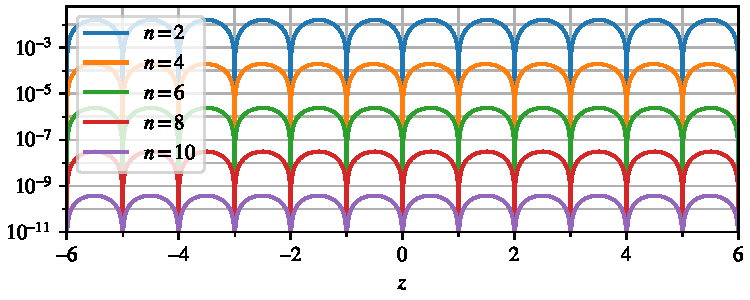
\includegraphics{papers/laguerre/images/rel_error_range.pdf}
%\vspace{-12pt}
\caption{Relativer Fehler des Ansatzes mit optimalen Verschiebungsterm
für verschiedene reele Werte von $z$ und Laguerre-Polynome vom Grad $n$}
\label{laguerre:fig:rel_error_range}
\end{figure}

\begin{figure}
\centering
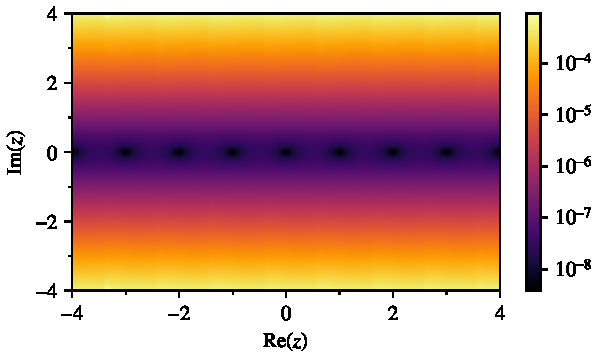
\includegraphics{papers/laguerre/images/rel_error_complex.pdf}
%\vspace{-12pt}
\caption{Absolutwert des relativen Fehlers in der komplexen Ebene}
\label{laguerre:fig:rel_error_complex}
\end{figure}

\subsubsection{Vergleich mit Lanczos-Methode}
Nun stellt sich die Frage,
wie das in diesem Abschnitt beschriebene Approximationsverfahren
der Gamma-Funktion sich gegenüber den üblichen Approximationsverfahren schlägt.
Eine häufig verwendete Methode ist die Lanczos-Approximation,
welche gegeben ist durch
\begin{align}
\Gamma(z + 1)
\approx
\sqrt{2\pi} \left( z + \sigma + \frac{1}{2} \right)^{z + 1/2}
e^{-(z + \sigma + 1/2)} \sum_{k=0}^n g_k H_k(z)
,
\end{align}
wobei
\begin{align*}
g_k = \frac{e^\sigma \varepsilon_k (-1)^k}{\sqrt{2\pi}}
\sum_{r=0}^k (-1)^r \, \binom{k}{r} \, (k)_r
\left( \frac{e}{r + \sigma + \frac{1}{2}}\right)^{r + 1/2}
,
\end{align*}
\begin{align*}
\varepsilon_k
=
\begin{cases}
1 & \text{für } k = 0 \\
2 & \text{sonst}
\end{cases}
\quad \text{und}\quad
H_k(z)
=
\frac{(-1)^k (-z)_k}{(z+1)_k}
\end{align*}
mit $H_0 = 1$ und $\sum_0^n g_k = 1$ (siehe \cite{laguerre:lanczos}).
Diese Methode wurde zum Beispiel in 
{\em GNU Scientific Library}, {\em Boost}, {\em CPython} und 
{\em musl} implementiert.
Diese Methode erreicht für $n = 7$ typischerweise Genauigkeit von $13$
korrekten, signifikanten Stellen für reele Argumente.
Zum Vergleich: die vorgestellte Methode erreicht für $n = 7$ 
eine minimale Genauigkeit von $6$ korrekten, signifikanten Stellen 
für reele Argumente.
Das Resultat ist etwas enttäuschend,
aber nicht unerwartet,
da die Lanczos-Methode spezifisch auf dieses Problem zugeschnitten ist und 
unsere Methode eine erweiterte allgemeine Methode ist.
Was die Komplexität der Berechnungen im Betrieb angeht,
ist die Gauss-Laguerre-Quadratur wesentlich ressourcensparender,
weil sie nur aus $n$ Funktionsevaluationen, 
wenigen Multiplikationen und Additionen besteht.
Demzufolge könnte diese Methode Anwendung in Systemen mit wenig Rechenleistung
und/oder knappen Energieressourcen finden.